% Options for packages loaded elsewhere
\PassOptionsToPackage{unicode}{hyperref}
\PassOptionsToPackage{hyphens}{url}
\PassOptionsToPackage{dvipsnames,svgnames,x11names}{xcolor}
%
\documentclass[
  letterpaper,
  DIV=11,
  numbers=noendperiod]{scrreport}

\usepackage{amsmath,amssymb}
\usepackage{lmodern}
\usepackage{iftex}
\ifPDFTeX
  \usepackage[T1]{fontenc}
  \usepackage[utf8]{inputenc}
  \usepackage{textcomp} % provide euro and other symbols
\else % if luatex or xetex
  \usepackage{unicode-math}
  \defaultfontfeatures{Scale=MatchLowercase}
  \defaultfontfeatures[\rmfamily]{Ligatures=TeX,Scale=1}
\fi
% Use upquote if available, for straight quotes in verbatim environments
\IfFileExists{upquote.sty}{\usepackage{upquote}}{}
\IfFileExists{microtype.sty}{% use microtype if available
  \usepackage[]{microtype}
  \UseMicrotypeSet[protrusion]{basicmath} % disable protrusion for tt fonts
}{}
\makeatletter
\@ifundefined{KOMAClassName}{% if non-KOMA class
  \IfFileExists{parskip.sty}{%
    \usepackage{parskip}
  }{% else
    \setlength{\parindent}{0pt}
    \setlength{\parskip}{6pt plus 2pt minus 1pt}}
}{% if KOMA class
  \KOMAoptions{parskip=half}}
\makeatother
\usepackage{xcolor}
\usepackage[normalem]{ulem}
\setlength{\emergencystretch}{3em} % prevent overfull lines
\setcounter{secnumdepth}{5}
% Make \paragraph and \subparagraph free-standing
\ifx\paragraph\undefined\else
  \let\oldparagraph\paragraph
  \renewcommand{\paragraph}[1]{\oldparagraph{#1}\mbox{}}
\fi
\ifx\subparagraph\undefined\else
  \let\oldsubparagraph\subparagraph
  \renewcommand{\subparagraph}[1]{\oldsubparagraph{#1}\mbox{}}
\fi

\usepackage{color}
\usepackage{fancyvrb}
\newcommand{\VerbBar}{|}
\newcommand{\VERB}{\Verb[commandchars=\\\{\}]}
\DefineVerbatimEnvironment{Highlighting}{Verbatim}{commandchars=\\\{\}}
% Add ',fontsize=\small' for more characters per line
\usepackage{framed}
\definecolor{shadecolor}{RGB}{241,243,245}
\newenvironment{Shaded}{\begin{snugshade}}{\end{snugshade}}
\newcommand{\AlertTok}[1]{\textcolor[rgb]{0.68,0.00,0.00}{#1}}
\newcommand{\AnnotationTok}[1]{\textcolor[rgb]{0.37,0.37,0.37}{#1}}
\newcommand{\AttributeTok}[1]{\textcolor[rgb]{0.40,0.45,0.13}{#1}}
\newcommand{\BaseNTok}[1]{\textcolor[rgb]{0.68,0.00,0.00}{#1}}
\newcommand{\BuiltInTok}[1]{\textcolor[rgb]{0.00,0.23,0.31}{#1}}
\newcommand{\CharTok}[1]{\textcolor[rgb]{0.13,0.47,0.30}{#1}}
\newcommand{\CommentTok}[1]{\textcolor[rgb]{0.37,0.37,0.37}{#1}}
\newcommand{\CommentVarTok}[1]{\textcolor[rgb]{0.37,0.37,0.37}{\textit{#1}}}
\newcommand{\ConstantTok}[1]{\textcolor[rgb]{0.56,0.35,0.01}{#1}}
\newcommand{\ControlFlowTok}[1]{\textcolor[rgb]{0.00,0.23,0.31}{#1}}
\newcommand{\DataTypeTok}[1]{\textcolor[rgb]{0.68,0.00,0.00}{#1}}
\newcommand{\DecValTok}[1]{\textcolor[rgb]{0.68,0.00,0.00}{#1}}
\newcommand{\DocumentationTok}[1]{\textcolor[rgb]{0.37,0.37,0.37}{\textit{#1}}}
\newcommand{\ErrorTok}[1]{\textcolor[rgb]{0.68,0.00,0.00}{#1}}
\newcommand{\ExtensionTok}[1]{\textcolor[rgb]{0.00,0.23,0.31}{#1}}
\newcommand{\FloatTok}[1]{\textcolor[rgb]{0.68,0.00,0.00}{#1}}
\newcommand{\FunctionTok}[1]{\textcolor[rgb]{0.28,0.35,0.67}{#1}}
\newcommand{\ImportTok}[1]{\textcolor[rgb]{0.00,0.46,0.62}{#1}}
\newcommand{\InformationTok}[1]{\textcolor[rgb]{0.37,0.37,0.37}{#1}}
\newcommand{\KeywordTok}[1]{\textcolor[rgb]{0.00,0.23,0.31}{#1}}
\newcommand{\NormalTok}[1]{\textcolor[rgb]{0.00,0.23,0.31}{#1}}
\newcommand{\OperatorTok}[1]{\textcolor[rgb]{0.37,0.37,0.37}{#1}}
\newcommand{\OtherTok}[1]{\textcolor[rgb]{0.00,0.23,0.31}{#1}}
\newcommand{\PreprocessorTok}[1]{\textcolor[rgb]{0.68,0.00,0.00}{#1}}
\newcommand{\RegionMarkerTok}[1]{\textcolor[rgb]{0.00,0.23,0.31}{#1}}
\newcommand{\SpecialCharTok}[1]{\textcolor[rgb]{0.37,0.37,0.37}{#1}}
\newcommand{\SpecialStringTok}[1]{\textcolor[rgb]{0.13,0.47,0.30}{#1}}
\newcommand{\StringTok}[1]{\textcolor[rgb]{0.13,0.47,0.30}{#1}}
\newcommand{\VariableTok}[1]{\textcolor[rgb]{0.07,0.07,0.07}{#1}}
\newcommand{\VerbatimStringTok}[1]{\textcolor[rgb]{0.13,0.47,0.30}{#1}}
\newcommand{\WarningTok}[1]{\textcolor[rgb]{0.37,0.37,0.37}{\textit{#1}}}

\providecommand{\tightlist}{%
  \setlength{\itemsep}{0pt}\setlength{\parskip}{0pt}}\usepackage{longtable,booktabs,array}
\usepackage{calc} % for calculating minipage widths
% Correct order of tables after \paragraph or \subparagraph
\usepackage{etoolbox}
\makeatletter
\patchcmd\longtable{\par}{\if@noskipsec\mbox{}\fi\par}{}{}
\makeatother
% Allow footnotes in longtable head/foot
\IfFileExists{footnotehyper.sty}{\usepackage{footnotehyper}}{\usepackage{footnote}}
\makesavenoteenv{longtable}
\usepackage{graphicx}
\makeatletter
\def\maxwidth{\ifdim\Gin@nat@width>\linewidth\linewidth\else\Gin@nat@width\fi}
\def\maxheight{\ifdim\Gin@nat@height>\textheight\textheight\else\Gin@nat@height\fi}
\makeatother
% Scale images if necessary, so that they will not overflow the page
% margins by default, and it is still possible to overwrite the defaults
% using explicit options in \includegraphics[width, height, ...]{}
\setkeys{Gin}{width=\maxwidth,height=\maxheight,keepaspectratio}
% Set default figure placement to htbp
\makeatletter
\def\fps@figure{htbp}
\makeatother

\usepackage{booktabs}
\usepackage{longtable}
\usepackage{array}
\usepackage{multirow}
\usepackage{wrapfig}
\usepackage{float}
\usepackage{colortbl}
\usepackage{pdflscape}
\usepackage{tabu}
\usepackage{threeparttable}
\usepackage{threeparttablex}
\usepackage[normalem]{ulem}
\usepackage{makecell}
\usepackage{xcolor}
\usepackage{makeidx}
\makeindex
\KOMAoption{captions}{tableheading}
\makeatletter
\@ifpackageloaded{tcolorbox}{}{\usepackage[many]{tcolorbox}}
\@ifpackageloaded{fontawesome5}{}{\usepackage{fontawesome5}}
\definecolor{quarto-callout-color}{HTML}{909090}
\definecolor{quarto-callout-note-color}{HTML}{0758E5}
\definecolor{quarto-callout-important-color}{HTML}{CC1914}
\definecolor{quarto-callout-warning-color}{HTML}{EB9113}
\definecolor{quarto-callout-tip-color}{HTML}{00A047}
\definecolor{quarto-callout-caution-color}{HTML}{FC5300}
\definecolor{quarto-callout-color-frame}{HTML}{acacac}
\definecolor{quarto-callout-note-color-frame}{HTML}{4582ec}
\definecolor{quarto-callout-important-color-frame}{HTML}{d9534f}
\definecolor{quarto-callout-warning-color-frame}{HTML}{f0ad4e}
\definecolor{quarto-callout-tip-color-frame}{HTML}{02b875}
\definecolor{quarto-callout-caution-color-frame}{HTML}{fd7e14}
\makeatother
\makeatletter
\makeatother
\makeatletter
\@ifpackageloaded{bookmark}{}{\usepackage{bookmark}}
\makeatother
\makeatletter
\@ifpackageloaded{caption}{}{\usepackage{caption}}
\AtBeginDocument{%
\ifdefined\contentsname
  \renewcommand*\contentsname{Table of contents}
\else
  \newcommand\contentsname{Table of contents}
\fi
\ifdefined\listfigurename
  \renewcommand*\listfigurename{List of Figures}
\else
  \newcommand\listfigurename{List of Figures}
\fi
\ifdefined\listtablename
  \renewcommand*\listtablename{List of Tables}
\else
  \newcommand\listtablename{List of Tables}
\fi
\ifdefined\figurename
  \renewcommand*\figurename{Figure}
\else
  \newcommand\figurename{Figure}
\fi
\ifdefined\tablename
  \renewcommand*\tablename{Table}
\else
  \newcommand\tablename{Table}
\fi
}
\@ifpackageloaded{float}{}{\usepackage{float}}
\floatstyle{ruled}
\@ifundefined{c@chapter}{\newfloat{codelisting}{h}{lop}}{\newfloat{codelisting}{h}{lop}[chapter]}
\floatname{codelisting}{Listing}
\newcommand*\listoflistings{\listof{codelisting}{List of Listings}}
\makeatother
\makeatletter
\@ifpackageloaded{caption}{}{\usepackage{caption}}
\@ifpackageloaded{subcaption}{}{\usepackage{subcaption}}
\makeatother
\makeatletter
\@ifpackageloaded{tcolorbox}{}{\usepackage[many]{tcolorbox}}
\makeatother
\makeatletter
\@ifundefined{shadecolor}{\definecolor{shadecolor}{rgb}{.97, .97, .97}}
\makeatother
\makeatletter
\makeatother
\ifLuaTeX
  \usepackage{selnolig}  % disable illegal ligatures
\fi
\IfFileExists{bookmark.sty}{\usepackage{bookmark}}{\usepackage{hyperref}}
\IfFileExists{xurl.sty}{\usepackage{xurl}}{} % add URL line breaks if available
\urlstyle{same} % disable monospaced font for URLs
\hypersetup{
  pdftitle={Fiscal Futures Project},
  pdfauthor={Alea Wilbur-Mujtaba},
  colorlinks=true,
  linkcolor={blue},
  filecolor={Maroon},
  citecolor={Blue},
  urlcolor={Blue},
  pdfcreator={LaTeX via pandoc}}

\title{Fiscal Futures Project}
\author{Alea Wilbur-Mujtaba}
\date{2/8/23}

\begin{document}
\maketitle
\ifdefined\Shaded\renewenvironment{Shaded}{\begin{tcolorbox}[sharp corners, enhanced, interior hidden, frame hidden, borderline west={3pt}{0pt}{shadecolor}, boxrule=0pt, breakable]}{\end{tcolorbox}}\fi

\renewcommand*\contentsname{Table of contents}
{
\hypersetup{linkcolor=}
\setcounter{tocdepth}{2}
\tableofcontents
}
\bookmarksetup{startatroot}

\hypertarget{sec-background-info}{%
\chapter*{Background Information}\label{sec-background-info}}
\addcontentsline{toc}{chapter}{Background Information}

\markboth{Background Information}{Background Information}

\begin{quote}
This document is UNFINISHED. Every section is a work in progress and
will continue to be updated. - AWM 1/9/2023
\end{quote}

This is a living document in which we aim to describe things as clearly
as possible in the time we have, share it with others, and improve as we
come back to it. If we wait till we have time to write flawless docs,
it'll never happen.

Code and information on the analysis of Illinois' expenditures and
revenues. The Fiscal Future Project is associated with the Institute of
Government and Policy Affairs but publicly sharing the code and creating
a website was done by Alea Wilbur-Mujtaba. Any errors with code or
findings are the fault of the author, not the research institute. Data
originally from annual FOIA requests to the Illinois Office of the
Comptroller.

\hypertarget{including-or-excluding-funds-in-the-fiscal-futures-all-funds-budget}{%
\section*{Including or Excluding funds in the Fiscal Futures All Funds
Budget}\label{including-or-excluding-funds-in-the-fiscal-futures-all-funds-budget}}
\addcontentsline{toc}{section}{Including or Excluding funds in the
Fiscal Futures All Funds Budget}

\markright{Including or Excluding funds in the Fiscal Futures All Funds
Budget}

While it is called an ``All Funds'' Budget, that is a slight
exaggeration. Illinois has over 700 funds. Whereas the overwhelming
majority are included in our ``All Funds'' measure, some are not.~ The
starting point for our list of all funds is all appropriated funds, but,
for the reasons listed below, we exclude a handful of appropriated funds
and include a number of non-appropriated funds.~

\textbf{Criterion 1:~INCLUDE IF the fund collects a state-levied tax.}

The state collects both state-levied taxes and locally levied taxes
(typically local-option sales and utility taxes).~ The state collects
and returns local taxes to the local governments.~ Upon receipt, local
tax revenues are deposited into specifically-designated,
non-appropriated state trust funds.~ In cases where the state is solely
acting as a collection agent for a local taxing body, this receiving
trust fund, its revenue and distribution (expenditure) is NOT counted in
our analytical frame.~ If the tax is collected for the state, the fund
and its revenue IS counted in our analytical frame.~

\textbf{Criterion 2:~ INCLUDE IF the fund supports a state function.}

Non-appropriated funds may support state functions such as education,
social services, transportation, public facilities, regulation, natural
resources, and law enforcement.~ Generally these are trust funds that
hold federal dollars for a specified state project or purpose.~ This
category of \emph{non-appropriated} funds is essentially the same as a
large group of \emph{appropriated} state and federal trust funds.~
Because we are counting federal dollars as revenue, it would be
inconsistent to count the appropriated funds, but not the
non-appropriated funds that do essentially the same thing.~

\textbf{Criterion 3:~ EXCLUDE IF the fund is a holding fund for
individuals.}

Many funds are used to hold monies that belong to individuals, not the
state.~ Most of these funds are non-appropriated, but some are
appropriated.~ Examples of appropriated funds that we exclude from the
frame are child support collection funds or employee pension
own-contribution funds.~ These funds are holding money that belongs to
an individual and will be returned to the person, or used for a payment
on behalf of that person, at a later date.~

\textbf{Criterion 4:~ EXCLUDE IF the fund's expenditures or revenues
have been counted elsewhere (i.e., avoid double-counting).}

In some cases, funds receive and disburse money that was already counted
as revenues to or expenditures from other funds.~ For example, the
Commercial Consolidation Fund is a huge fund that distributes state
benefit payments to individuals, service providers, and local
governments by direct deposit.~ Payments into this fund are counted,
distributions from this fund are not.~

\textbf{Criterion 5:~ EXCLUDE IF the fund holds designated user fees
targeted for a specific purpose that is not a public function
(conduit).}

Typically we have excluded non-appropriated funds that hold designated
user fees that are directed to a specific purpose that is not a
necessary public function.~ These funds can be considered a conduit and
we did not add these to the frame. ~For example, we exclude Fund 0098,
which collects fees from harness race entrants at the state fair and
then pays them out to race winners.

\textbf{Criterion 6:~ INCLUDE IF the fund collects a user fee that
supports a large, important state function (state function trumps user
fee).}

Non-appropriated funds that are supported by user fees AND perform a
state function (e.g., transportation) ARE counted in the frame.~ The
rationale for this is that the state function would have to be performed
even if the user fee and the fund structure did not exist.~ The biggest
example is the Illinois State Toll Highway Revenue Fund, which collects
tolls and supports the expansion and maintenance of Illinois toll
roads.~

\textbf{Criterion 7:~ EXCLUDE IF unclear information, dead fund, small
amounts.} Some funds are defunct, and our historical information on fund
descriptions does not include pre-2005 designations. Fund numbers are
re-used, making it impossible to determine the original purpose of some
older, defunct funds.~ These funds generally appear to be very small.~
Because we are projecting forward from the most recently completed
fiscal year, we assumed that these funds would not be in the frame.~

\hypertarget{section}{%
\section*{}\label{section}}
\addcontentsline{toc}{section}{}

\markright{}

\bookmarksetup{startatroot}

\hypertarget{sec-gathering-and-cleaning-data}{%
\chapter{Gathering and Cleaning
Data!}\label{sec-gathering-and-cleaning-data}}

Information for the Fiscal Futures all funds database comes from
detailed information provided by the Illinois Comptroller's office.~
Currently the database includes 300,000 individual records for fiscal
years 1998 to 2022.

\begin{itemize}
\tightlist
\item
  Do the FOIA request. In a week or so, they send the expenditure and
  revenue data as excel files.
\item
  Checks whether there are any new agencies, re-used funds etc. Create a
  list of funds, agencies, fund names, etc. for the new year and compare
  it to the immediate prior year to identify new funds.
\item
  Update the funds\_ab\_in file which shows the use of funds. Use
  criteria to determine if the new funds should be in or out of the
  all-funds frame.
\item
  Change the variable names to be consistent with other files such as
  AGENCYNAME -\/-\textgreater{} agency\_name
\item
  Once variable names are shared over all years of data, combine past
  years with newest year. All revenue files are in a `revenue` folder
  that I reference when I set the working directory. When adding new
  fiscal years, put the the newest year of data for revenue and
  expenditures in their respective folders.
\end{itemize}

Normally, when your receive the new fiscal year files from the
Comptrollers office, you will need to change the variable names so that
they are consistent with past years. This is an example of reading in
the new file and changing the variable names. They seem to change almost
every year in the file received from the FOIA so if the code breaks
here, check to make sure that the columns you are trying to rename exist
and are spelled correctly! Once variables are the same, you will want to
save the file as a csv file in its Revenue/Expenditure file and bind all
past years and the current year together in one dataframe.

\begin{Shaded}
\begin{Highlighting}[]
\CommentTok{\#Example code below: Read in excel file and rename columns so that it plays well with the other years\textquotesingle{} files.}

\NormalTok{revenue\_fy22 }\OtherTok{\textless{}{-}} \FunctionTok{read\_xlsx}\NormalTok{(}\StringTok{"Fis\_Fut\_Rev\_2022\_Final.xlsx"}\NormalTok{) }\SpecialCharTok{\%\textgreater{}\%} 
  \FunctionTok{rename}\NormalTok{(}\AttributeTok{fy =} \StringTok{\textquotesingle{}FY\textquotesingle{}}\NormalTok{,}
         \AttributeTok{fund =} \StringTok{\textquotesingle{}FUND\textquotesingle{}}\NormalTok{,}
         \AttributeTok{fund\_name =} \StringTok{\textquotesingle{}FUND NAME\textquotesingle{}}\NormalTok{,}
         \AttributeTok{agency =} \StringTok{\textquotesingle{}AGENCY\textquotesingle{}}\NormalTok{,}
         \AttributeTok{agency\_name =} \StringTok{\textquotesingle{}AGENCY NAME\textquotesingle{}}\NormalTok{,}
         \AttributeTok{source =} \StringTok{\textquotesingle{}REVENUE SOURCE\textquotesingle{}}\NormalTok{,}
         \AttributeTok{source\_name =} \StringTok{\textquotesingle{}REV SRC NAME\textquotesingle{}}\NormalTok{,}
         \AttributeTok{receipts =} \StringTok{\textquotesingle{}AMOUNT\textquotesingle{}}
\NormalTok{  ) }

\NormalTok{exp\_fy22 }\OtherTok{\textless{}{-}} \FunctionTok{read\_xlsx}\NormalTok{(}\StringTok{"Fis\_Fut\_Exp\_2022\_Final.xlsx"}\NormalTok{) }\SpecialCharTok{\%\textgreater{}\%} 
  \FunctionTok{rename}\NormalTok{(}\AttributeTok{fy =} \StringTok{\textquotesingle{}FY\textquotesingle{}}\NormalTok{,}
         \AttributeTok{fund =} \StringTok{\textquotesingle{}FUND\textquotesingle{}}\NormalTok{,}
         \AttributeTok{fund\_name =} \StringTok{\textquotesingle{}FUND NAME\textquotesingle{}}\NormalTok{,}
         \AttributeTok{agency =} \StringTok{\textquotesingle{}AGENCY\textquotesingle{}}\NormalTok{,}
         \AttributeTok{agency\_name =} \StringTok{\textquotesingle{}AGENCY NAME\textquotesingle{}}\NormalTok{,}
         \AttributeTok{appr\_org =} \StringTok{\textquotesingle{}ORGANIZATION\textquotesingle{}}\NormalTok{,}
         \AttributeTok{org\_name =} \StringTok{\textquotesingle{}ORGANIZATION NAME\textquotesingle{}}\NormalTok{,}
         \AttributeTok{obj\_seq\_type =} \StringTok{\textquotesingle{}APPROPRIATION\textquotesingle{}}\NormalTok{,}
         \AttributeTok{wh\_approp\_name =} \StringTok{\textquotesingle{}APPROPRIATION NAME\textquotesingle{}}\NormalTok{,}
        \CommentTok{\# exp\_net\_xfer = \textquotesingle{}NET OF TRANS AMOUNT\textquotesingle{},}
         \AttributeTok{expenditure =} \StringTok{\textquotesingle{}EXPENDED\textquotesingle{}}

\NormalTok{  ) }

\CommentTok{\# \%\textgreater{}\%}
\CommentTok{\#   \# these come from ioc\_source file after merging}
\CommentTok{\#   mutate(data\_source = "exp IOC Aug 2022",}
\CommentTok{\#          object = ,}
\CommentTok{\#          seq = ,}
\CommentTok{\#          type = ,}
\CommentTok{\#          fund\_cat = FIND\_COLUMN, \#create fund\_cat column}
\CommentTok{\#          fund\_cat\_name = FIND\_NAME) \# create fund\_cat\_name column}
\end{Highlighting}
\end{Shaded}

The code chunk below takes the .dta files for all fiscal years before FY
2022 and binds them together. Variable names were manually changed by
past researchers so that they were consistent across years.

For FY 2023 and after, .dta files can be avoided entirely and .csv or
excel files will be used. All files before this year had been saved and
passed on as .dta files for Stata code before the transition to R in
Fall 2022. For years after fy22: add line of code to bind csv files
after binding the dta files together. Variable names must identical to
merge files together.

Code below reads in the csv files created in chunks above
(allrevfiles.csv and allrexpfiles.csv). These files contain all years of
data combined into one file BEFORE any recoding is done. Do not use this
file for summing categories because it is just an inbetween step before
recoding revenue and expenditure categories.

\begin{Shaded}
\begin{Highlighting}[]
\CommentTok{\# combined in past chunks called create{-}rev{-}csv and create{-}exp{-}csv}

\NormalTok{allrevfiles22 }\OtherTok{\textless{}{-}} \FunctionTok{read\_csv}\NormalTok{(}\StringTok{"allrevfiles22.csv"}\NormalTok{) }\CommentTok{\#combined but not recoded}

\NormalTok{allexpfiles22 }\OtherTok{\textless{}{-}} \FunctionTok{read\_csv}\NormalTok{(}\StringTok{"allexpfiles22.csv"}\NormalTok{) }\CommentTok{\#combined but not recoded}
\end{Highlighting}
\end{Shaded}

\hypertarget{inspecting-new-fy22-data-files}{%
\subsection{Inspecting new FY22 data
files}\label{inspecting-new-fy22-data-files}}

Data files for closed years have been obtained from IOC. The numbers of
funds, agencies, organizations, and revenue sources below were found by
using pivot tables in the codebook files in the FY2022 Box folder. This
could also be done using R and grouping new files by fund, agency,
source number, source names, etc..

Revenue File:

\begin{itemize}
\tightlist
\item
  684 Fund Numbers
\item
  80 Agencies
\item
  1184 Revenue source numbers
\item
  1156 revenue source names
\end{itemize}

Expenditure File:

\begin{itemize}
\tightlist
\item
  708 Fund Numbers
\item
  107 Agencies
\item
  98 Organization Numbers
\item
  313 Organization names
\end{itemize}

\hypertarget{finding-new-agencies-and-funds}{%
\subsection{Finding new agencies and
funds}\label{finding-new-agencies-and-funds}}

General steps:

\begin{enumerate}
\def\labelenumi{\arabic{enumi}.}
\tightlist
\item
  Identify new and reused funds for newest fiscal year.
\item
  Recode funds to take into account different fund numbers/names over
  the years. See {[}Recoding New and Reused Funds{]} for code chunk that
  does this.
\item
  Update fund\_ab\_in\_2022.xlsx with any changes from previous fiscal
  year.
\end{enumerate}

\textbf{New Agencies, Funds, and Organizations from Expenditure files:}

\begin{itemize}
\tightlist
\item
  Using the code below, I found 2 agencies, multiple funds, and a couple
  organizations that had not been specifically mentioned in the
  funds\_ab\_in file - AWM, FY2022.
\item
  Note: One new org name and org number combo has an expenditure of
  \$600 million for pensions payment. Investigate later.
\end{itemize}

\begin{Shaded}
\begin{Highlighting}[]
\NormalTok{allrevfiles22 }\OtherTok{\textless{}{-}} \FunctionTok{read\_csv}\NormalTok{(}\StringTok{"allrevfiles22.csv"}\NormalTok{) }\CommentTok{\#combined but not recoded}

\NormalTok{allexpfiles22 }\OtherTok{\textless{}{-}} \FunctionTok{read\_csv}\NormalTok{(}\StringTok{"allexpfiles22.csv"}\NormalTok{) }\CommentTok{\#combined but not recoded}


\DocumentationTok{\#\#\#\# From Expenditure Data \#\#\#\#\#}

\CommentTok{\# agencies referenced in any year before 2020:}

\NormalTok{agencies\_past }\OtherTok{\textless{}{-}}\NormalTok{ allexpfiles22 }\SpecialCharTok{\%\textgreater{}\%} 
  \FunctionTok{filter}\NormalTok{(fy }\SpecialCharTok{\textless{}} \DecValTok{2022}\NormalTok{) }\SpecialCharTok{\%\textgreater{}\%} 
  \FunctionTok{mutate}\NormalTok{(agency }\SpecialCharTok{==} \FunctionTok{as.character}\NormalTok{(agency)) }\SpecialCharTok{\%\textgreater{}\%} 
  \FunctionTok{group\_by}\NormalTok{(agency, agency\_name) }\SpecialCharTok{\%\textgreater{}\%} 
  \FunctionTok{unique}\NormalTok{() }\SpecialCharTok{\%\textgreater{}\%} 
  \FunctionTok{summarize}\NormalTok{(}\AttributeTok{expenditure =} \FunctionTok{sum}\NormalTok{(expenditure, }\AttributeTok{na.rm =} \ConstantTok{TRUE}\NormalTok{)) }\SpecialCharTok{\%\textgreater{}\%} 
  \FunctionTok{drop\_na}\NormalTok{() }\SpecialCharTok{\%\textgreater{}\%} 
  \FunctionTok{arrange}\NormalTok{(agency)}

\CommentTok{\# agencies\_past \# 146 agencies ever}

\CommentTok{\# agencies in 2022 data:}

\NormalTok{agencies22 }\OtherTok{\textless{}{-}}\NormalTok{ allexpfiles22  }\SpecialCharTok{\%\textgreater{}\%} 
  \FunctionTok{filter}\NormalTok{(fy }\SpecialCharTok{==} \DecValTok{2022}\NormalTok{) }\SpecialCharTok{\%\textgreater{}\%} 
  \FunctionTok{mutate}\NormalTok{(agency }\SpecialCharTok{==} \FunctionTok{as.character}\NormalTok{(agency)) }\SpecialCharTok{\%\textgreater{}\%} 
  \FunctionTok{group\_by}\NormalTok{(agency, agency\_name) }\SpecialCharTok{\%\textgreater{}\%} 
  \FunctionTok{summarize}\NormalTok{(}\AttributeTok{expenditure =} \FunctionTok{sum}\NormalTok{(expenditure, }\AttributeTok{na.rm =} \ConstantTok{TRUE}\NormalTok{))}

\CommentTok{\# agencies22 \# 107 agencies this year}

\CommentTok{\# 280 and 533 are new agency codes: }

\FunctionTok{anti\_join}\NormalTok{(agencies22, agencies\_past, }
          \AttributeTok{by =} \FunctionTok{c}\NormalTok{(}\StringTok{"agency"}\NormalTok{, }\StringTok{"agency\_name"}\NormalTok{)) }\SpecialCharTok{\%\textgreater{}\%} 
  \FunctionTok{arrange}\NormalTok{(agency)}
\end{Highlighting}
\end{Shaded}

\begin{verbatim}
# A tibble: 2 x 3
# Groups:   agency [2]
  agency agency_name                expenditure
   <dbl> <chr>                            <dbl>
1    280 COURTS COMMISSION               37747.
2    533 COMM ON EQUITY & INCLUSION    1405788.
\end{verbatim}

\begin{Shaded}
\begin{Highlighting}[]
\NormalTok{funds\_past }\OtherTok{\textless{}{-}}\NormalTok{ allexpfiles22  }\SpecialCharTok{\%\textgreater{}\%} 
  \FunctionTok{filter}\NormalTok{(fy }\SpecialCharTok{\textless{}} \DecValTok{2022}\NormalTok{) }\SpecialCharTok{\%\textgreater{}\%} 
  \FunctionTok{mutate}\NormalTok{(fund }\SpecialCharTok{==} \FunctionTok{as.character}\NormalTok{(fund)) }\SpecialCharTok{\%\textgreater{}\%} 
  \FunctionTok{group\_by}\NormalTok{(fund, fund\_name) }\SpecialCharTok{\%\textgreater{}\%} 
  \FunctionTok{summarize}\NormalTok{(}\AttributeTok{count =} \FunctionTok{n}\NormalTok{(), }\AttributeTok{Expenditure =} \FunctionTok{sum}\NormalTok{(expenditure, }\AttributeTok{na.rm =} \ConstantTok{TRUE}\NormalTok{))  }\SpecialCharTok{\%\textgreater{}\%} 
  \FunctionTok{drop\_na}\NormalTok{()}

\NormalTok{funds22 }\OtherTok{\textless{}{-}}\NormalTok{ allexpfiles22  }\SpecialCharTok{\%\textgreater{}\%} 
  \FunctionTok{filter}\NormalTok{(fy }\SpecialCharTok{==} \DecValTok{2022}\NormalTok{) }\SpecialCharTok{\%\textgreater{}\%} 
  \FunctionTok{mutate}\NormalTok{(fund }\SpecialCharTok{==} \FunctionTok{as.character}\NormalTok{(fund)) }\SpecialCharTok{\%\textgreater{}\%} 
  \FunctionTok{group\_by}\NormalTok{(fund, fund\_name) }\SpecialCharTok{\%\textgreater{}\%}  
  \FunctionTok{summarize}\NormalTok{(}\AttributeTok{count =} \FunctionTok{n}\NormalTok{(), }\AttributeTok{Expenditure =} \FunctionTok{sum}\NormalTok{(expenditure, }\AttributeTok{na.rm =} \ConstantTok{TRUE}\NormalTok{)) }\SpecialCharTok{\%\textgreater{}\%} 
  \FunctionTok{unique}\NormalTok{()}

\CommentTok{\# 15 funds were in FY22 data that were not in past data:}

\FunctionTok{anti\_join}\NormalTok{(funds22, funds\_past, }\AttributeTok{by =} \FunctionTok{c}\NormalTok{(}\StringTok{"fund"}\NormalTok{, }\StringTok{"fund\_name"}\NormalTok{)) }\SpecialCharTok{\%\textgreater{}\%} \FunctionTok{arrange}\NormalTok{(fund)}
\end{Highlighting}
\end{Shaded}

\begin{verbatim}
# A tibble: 15 x 4
# Groups:   fund [15]
   fund  fund_name                      count Expenditure
   <chr> <chr>                          <int>       <dbl>
 1 0110  DEV. DISABILITIES AWARENESS        1          0 
 2 0319  PENSION STABILIZATION             10  300000000 
 3 0351  FREEDOM SCHOOLS                    1     335306 
 4 0367  CAP FACILITY TEC MODERNIZATION     2    1000000 
 5 0392  EQUAL PAY REGISTRATION             1          0 
 6 0393  SICKLE CELL CHRONIC DISEASE        1          0 
 7 0422  ELECTRIC VEHICLE REBATE            3     225069.
 8 0427  ENERGY TRANSITION ASSISTANCE       8    6046483.
 9 0461  PARITY ADVANCEMENT                 1          0 
10 0544  DOIT SPECIAL PROJECTS              3    9998632.
11 0628  ESSENTIAL GOVT SERV SUPPORT        1  736120867.
12 0634  STATE TREASURER'S CAPITAL          1     250000 
13 0656  HORSE RACING PURSE EQUITY          1    5908048.
14 0672  CONSUMER INTERVENOR COMP.          1       2665 
15 0976  FAIRGROUNDS IMPROVMNT & RACING     1      10000 
\end{verbatim}

\begin{Shaded}
\begin{Highlighting}[]
\CommentTok{\# orgs\_pastin the past =  916 org groups ever}

\NormalTok{orgs\_past }\OtherTok{\textless{}{-}}\NormalTok{ allexpfiles22  }\SpecialCharTok{\%\textgreater{}\%} 
  \FunctionTok{filter}\NormalTok{(fy }\SpecialCharTok{\textless{}} \DecValTok{2022}\NormalTok{) }\SpecialCharTok{\%\textgreater{}\%} 
  \FunctionTok{mutate}\NormalTok{(appr\_org }\SpecialCharTok{==} \FunctionTok{as.character}\NormalTok{(appr\_org)) }\SpecialCharTok{\%\textgreater{}\%} 
  \FunctionTok{group\_by}\NormalTok{(appr\_org, org\_name) }\SpecialCharTok{\%\textgreater{}\%} 
  \FunctionTok{unique}\NormalTok{() }\SpecialCharTok{\%\textgreater{}\%} 
  \FunctionTok{summarize}\NormalTok{(}\AttributeTok{Expenditure =} \FunctionTok{sum}\NormalTok{(expenditure, }\AttributeTok{na.rm =} \ConstantTok{TRUE}\NormalTok{)) }\SpecialCharTok{\%\textgreater{}\%} \FunctionTok{drop\_na}\NormalTok{()}

\CommentTok{\# orgs\_past \# 916 org groups ever}

\NormalTok{orgs22 }\OtherTok{\textless{}{-}}\NormalTok{ allexpfiles22  }\SpecialCharTok{\%\textgreater{}\%} 
  \FunctionTok{filter}\NormalTok{(fy }\SpecialCharTok{==} \DecValTok{2022}\NormalTok{) }\SpecialCharTok{\%\textgreater{}\%} 
  \FunctionTok{mutate}\NormalTok{(}\AttributeTok{appr\_org =} \FunctionTok{as.character}\NormalTok{(appr\_org)) }\SpecialCharTok{\%\textgreater{}\%} 
  \FunctionTok{group\_by}\NormalTok{(appr\_org, org\_name) }\SpecialCharTok{\%\textgreater{}\%} 
  \FunctionTok{summarize}\NormalTok{(}\AttributeTok{Expenditure =} \FunctionTok{sum}\NormalTok{(expenditure, }\AttributeTok{na.rm =} \ConstantTok{TRUE}\NormalTok{))}

\CommentTok{\# orgs22 \# 396 org groups this year}

\CommentTok{\# 4 org number and org name combos are new for FY2022:}

\FunctionTok{anti\_join}\NormalTok{(orgs22, orgs\_past, }\AttributeTok{by =} \FunctionTok{c}\NormalTok{(}\StringTok{"appr\_org"}\NormalTok{, }\StringTok{"org\_name"}\NormalTok{)) }\SpecialCharTok{\%\textgreater{}\%} \FunctionTok{arrange}\NormalTok{(appr\_org)}
\end{Highlighting}
\end{Shaded}

\begin{verbatim}
# A tibble: 4 x 3
# Groups:   appr_org [4]
  appr_org org_name                      Expenditure
  <chr>    <chr>                               <dbl>
1 05       PAROLE                          53426135.
2 06       RE-ENTRY SERVICES               18338411.
3 25       RETIREMENT SYSTEM PMT ADMIN    600000000 
4 34       IL CRIMINAL JUSTICE INFO AUTH      55659.
\end{verbatim}

\textbf{New Revenue Funds, Sources, and New Agencies:}

\begin{Shaded}
\begin{Highlighting}[]
\DocumentationTok{\#\#\#\# From Revenue Data \#\#\#\#}

\CommentTok{\# agencies\_past \# 108 agencies ever}

\NormalTok{agencies\_past }\OtherTok{\textless{}{-}}\NormalTok{ allrevfiles22  }\SpecialCharTok{\%\textgreater{}\%} 
  \FunctionTok{filter}\NormalTok{(fy }\SpecialCharTok{\textless{}} \DecValTok{2022}\NormalTok{) }\SpecialCharTok{\%\textgreater{}\%} 
  \FunctionTok{mutate}\NormalTok{(agency }\SpecialCharTok{==} \FunctionTok{as.character}\NormalTok{(agency)) }\SpecialCharTok{\%\textgreater{}\%} 
  \FunctionTok{group\_by}\NormalTok{(agency, agency\_name) }\SpecialCharTok{\%\textgreater{}\%} 
  \FunctionTok{unique}\NormalTok{() }\SpecialCharTok{\%\textgreater{}\%} 
  \FunctionTok{summarize}\NormalTok{(}\AttributeTok{Receipts =} \FunctionTok{sum}\NormalTok{(receipts, }\AttributeTok{na.rm =} \ConstantTok{TRUE}\NormalTok{)) }\SpecialCharTok{\%\textgreater{}\%} 
  \FunctionTok{drop\_na}\NormalTok{()}

\CommentTok{\# agencies22 \# 80 agencies this year}

\NormalTok{agencies22 }\OtherTok{\textless{}{-}}\NormalTok{ allrevfiles22  }\SpecialCharTok{\%\textgreater{}\%} 
  \FunctionTok{filter}\NormalTok{(fy }\SpecialCharTok{==} \DecValTok{2022}\NormalTok{) }\SpecialCharTok{\%\textgreater{}\%} 
  \FunctionTok{mutate}\NormalTok{(agency }\SpecialCharTok{==} \FunctionTok{as.character}\NormalTok{(agency)) }\SpecialCharTok{\%\textgreater{}\%} 
  \FunctionTok{group\_by}\NormalTok{(agency, agency\_name) }\SpecialCharTok{\%\textgreater{}\%} 
  \FunctionTok{summarize}\NormalTok{(}\AttributeTok{Receipts =} \FunctionTok{sum}\NormalTok{(receipts, }\AttributeTok{na.rm =} \ConstantTok{TRUE}\NormalTok{))}

\CommentTok{\# 0 new agencies in revenue data this year}

\FunctionTok{anti\_join}\NormalTok{(agencies22, agencies\_past, }\AttributeTok{by =} \FunctionTok{c}\NormalTok{(}\StringTok{"agency"}\NormalTok{, }\StringTok{"agency\_name"}\NormalTok{)) }\SpecialCharTok{\%\textgreater{}\%} \FunctionTok{arrange}\NormalTok{(agency)}
\end{Highlighting}
\end{Shaded}

\begin{verbatim}
# A tibble: 0 x 3
# Groups:   agency [0]
# ... with 3 variables: agency <dbl>, agency_name <chr>, Receipts <dbl>
\end{verbatim}

\begin{Shaded}
\begin{Highlighting}[]
\NormalTok{funds\_past }\OtherTok{\textless{}{-}}\NormalTok{ allrevfiles22  }\SpecialCharTok{\%\textgreater{}\%} 
  \FunctionTok{filter}\NormalTok{(fy }\SpecialCharTok{\textless{}} \DecValTok{2022}\NormalTok{) }\SpecialCharTok{\%\textgreater{}\%} 
  \FunctionTok{mutate}\NormalTok{(fund }\SpecialCharTok{==} \FunctionTok{as.character}\NormalTok{(fund)) }\SpecialCharTok{\%\textgreater{}\%} 
  \FunctionTok{group\_by}\NormalTok{(fund, fund\_name) }\SpecialCharTok{\%\textgreater{}\%} 
  \FunctionTok{summarize}\NormalTok{(}\AttributeTok{count =} \FunctionTok{n}\NormalTok{(), }\AttributeTok{Receipts =} \FunctionTok{sum}\NormalTok{(receipts, }\AttributeTok{na.rm =} \ConstantTok{TRUE}\NormalTok{))  }\SpecialCharTok{\%\textgreater{}\%} 
  \FunctionTok{drop\_na}\NormalTok{()}

\NormalTok{funds22 }\OtherTok{\textless{}{-}}\NormalTok{ allrevfiles22  }\SpecialCharTok{\%\textgreater{}\%} 
  \FunctionTok{filter}\NormalTok{(fy }\SpecialCharTok{==} \DecValTok{2022}\NormalTok{) }\SpecialCharTok{\%\textgreater{}\%} 
  \FunctionTok{mutate}\NormalTok{(fund }\SpecialCharTok{==} \FunctionTok{as.character}\NormalTok{(fund)) }\SpecialCharTok{\%\textgreater{}\%} 
  \FunctionTok{group\_by}\NormalTok{(fund, fund\_name) }\SpecialCharTok{\%\textgreater{}\%}  
  \FunctionTok{summarize}\NormalTok{(}\AttributeTok{count =} \FunctionTok{n}\NormalTok{(), }\AttributeTok{Receipts =} \FunctionTok{sum}\NormalTok{(receipts, }\AttributeTok{na.rm =} \ConstantTok{TRUE}\NormalTok{)) }\SpecialCharTok{\%\textgreater{}\%} 
  \FunctionTok{unique}\NormalTok{() }\SpecialCharTok{\%\textgreater{}\%} 
  \FunctionTok{drop\_na}\NormalTok{()}

\CommentTok{\# 19 revenue funds were in FY22 revenue data that were not in past data }

\CommentTok{\# some could be small fund name changes}

\FunctionTok{anti\_join}\NormalTok{(funds22, funds\_past, }\AttributeTok{by =} \FunctionTok{c}\NormalTok{(}\StringTok{"fund"}\NormalTok{, }\StringTok{"fund\_name"}\NormalTok{)) }\SpecialCharTok{\%\textgreater{}\%} \FunctionTok{arrange}\NormalTok{(fund)}
\end{Highlighting}
\end{Shaded}

\begin{verbatim}
# A tibble: 19 x 4
# Groups:   fund [19]
   fund  fund_name                      count    Receipts
   <chr> <chr>                          <int>       <dbl>
 1 0165  RONALD MCDONALD HOUSE CHARITY      1     143893.
 2 0319  PENSION STABILIZATION              1  300000000 
 3 0351  FREEDOM SCHOOLS                    1   17000000 
 4 0367  CAP FACILITY TEC MODERNIZATION     1    5300000 
 5 0392  EQUAL PAY REGISTRATION             1      24150 
 6 0422  ELECTRIC VEHICLE REBATE            3   13528800 
 7 0427  ENERGY TRANSITION ASSISTANCE       1   28773075.
 8 0544  DOIT SPECIAL PROJECTS              2    9998632.
 9 0628  ESSENTIAL GOVT SERV SUPPORT        1 1000000000 
10 0634  STATE TREASURER'S CAPITAL          2     273192.
11 0656  HORSE RACING PURSE EQUITY          1    5908048.
12 0672  CONSUMER INTERVENOR COMP.          1    1220000 
13 0683  GROCERY TAX REPLACEMENT            1  325000000 
14 0723  REVOCATION ENFORCEMENT             1     749073.
15 0742  ST. POLICE TRAINING & ACADEMY      1    2803359.
16 0743  LAW ENFORCEMENT TRAINING           1   25230230.
17 0848  SETTLEMENT                         1    5000000 
18 0966  ILLINOIS WORKS                     1   10000000 
19 0976  FAIRGROUNDS IMPROVMNT & RACING     3      93664.
\end{verbatim}

\begin{Shaded}
\begin{Highlighting}[]
\NormalTok{sources\_past }\OtherTok{\textless{}{-}}\NormalTok{ allrevfiles22  }\SpecialCharTok{\%\textgreater{}\%} 
  \FunctionTok{filter}\NormalTok{(fy }\SpecialCharTok{\textless{}} \DecValTok{2022}\NormalTok{) }\SpecialCharTok{\%\textgreater{}\%} 
  \FunctionTok{mutate}\NormalTok{(source }\SpecialCharTok{==} \FunctionTok{as.character}\NormalTok{(source)) }\SpecialCharTok{\%\textgreater{}\%} 
  \FunctionTok{group\_by}\NormalTok{(source, source\_name) }\SpecialCharTok{\%\textgreater{}\%} 
  \FunctionTok{summarize}\NormalTok{(}\AttributeTok{count =} \FunctionTok{n}\NormalTok{(), }\AttributeTok{Receipts =} \FunctionTok{sum}\NormalTok{(receipts, }\AttributeTok{na.rm =} \ConstantTok{TRUE}\NormalTok{))  }\SpecialCharTok{\%\textgreater{}\%} 
  \FunctionTok{drop\_na}\NormalTok{()}

\NormalTok{sources22 }\OtherTok{\textless{}{-}}\NormalTok{ allrevfiles22  }\SpecialCharTok{\%\textgreater{}\%} 
  \FunctionTok{filter}\NormalTok{(fy }\SpecialCharTok{==} \DecValTok{2022}\NormalTok{) }\SpecialCharTok{\%\textgreater{}\%} 
  \FunctionTok{mutate}\NormalTok{(source }\SpecialCharTok{==} \FunctionTok{as.character}\NormalTok{(source)) }\SpecialCharTok{\%\textgreater{}\%} 
  \FunctionTok{group\_by}\NormalTok{(source, source\_name) }\SpecialCharTok{\%\textgreater{}\%}  
  \FunctionTok{summarize}\NormalTok{(}\AttributeTok{count =} \FunctionTok{n}\NormalTok{(), }\AttributeTok{Receipts =} \FunctionTok{sum}\NormalTok{(receipts, }\AttributeTok{na.rm =} \ConstantTok{TRUE}\NormalTok{)) }\SpecialCharTok{\%\textgreater{}\%} 
  \FunctionTok{unique}\NormalTok{()}

\CommentTok{\# 20 revenue sources were in FY22 data that were not in past data }

\CommentTok{\# some could be small source name changes:}

\FunctionTok{anti\_join}\NormalTok{(sources22, sources\_past, }\AttributeTok{by =} \FunctionTok{c}\NormalTok{(}\StringTok{"source"}\NormalTok{, }\StringTok{"source\_name"}\NormalTok{)) }\SpecialCharTok{\%\textgreater{}\%} \FunctionTok{arrange}\NormalTok{(source)}
\end{Highlighting}
\end{Shaded}

\begin{verbatim}
# A tibble: 20 x 4
# Groups:   source [20]
   source source_name                    count   Receipts
   <chr>  <chr>                          <int>      <dbl>
 1 0303   LOTTERY-ILOTTERY SETTLEMENT        1 177417302.
 2 2292   VIDEO TERMINAL TAX                 3 893824162.
 3 2457   E ST LOUIS FINANCE AUTH            1     41667.
 4 2590   ALTON CENTER BUSINESS PARK         1    291667.
 5 2611   E-PAY ADMINISTRATION FEES          1   1136121.
 6 2660   CONCESSION REVENUE-FOOD            1     17210.
 7 2682   SW BADGE REPLACEMENT FEES          1        10 
 8 2699   RB RECONCILIATION FEE              1  15000000 
 9 2729   NORTH PARK COLLEGE LIC PLATES      1        20 
10 2736   STATE ST INSTITNL US GOV FND       1   1622448.
11 2737   VGA - IL STATE FAIR OP FEES        1     48387.
12 2738   VGA-DU QUOIN STATE FAIR OP FEE     1     11029.
13 2739   PUBLIC UTILITIES                   1   1220000 
14 2740   ENRGY TRANSITION ASST/ELECTRIC     1  28773075.
15 2742   OPERATION ASSESSMENT FEE           1   2828085.
16 2745   FY22 TITLE INCREASE                1   3072054 
17 2747   BUSINESS FILING FEE                1     24150 
18 2748   CORN COMMODITY SPONSORS            1      5000 
19 2755   PUBLIC UTIL - ETHICS REPRT FEE     1   1235000 
20 2756   UNEXP CAPITAL IMP PROJECTS         1     90583.
\end{verbatim}

Sources 2737 through 2756 were not found in the IOC\_source file so I
added them to \texttt{ioc\_source\_updated22\_AWM.xlsx}. Revenue source
types were found manually using the Comptroller's website and searching
for each source listed above and identifying its type. Then the
ioc\_source excel file was updated to include the revenue type
(Completed Jan.~20 2023, AFTER the FY22 paper totals were calculated.
There were very minor differences in aggregated expenditures and
revenues.) \texttt{ioc\_source\_updated22\_AWM.xlsx} will become the
generic \texttt{ioc\_source.xlsx} file in the future.

\hypertarget{recoding-new-and-reused-funds}{%
\subsection{Recoding New and Reused
Funds}\label{recoding-new-and-reused-funds}}

New funds will need to be manually added to the funds\_ab\_in excel file
and determined if they should or should not be included in Fiscal Future
calculations.

For funds that were reused once, a 9 replaces the 0 as the first digit.
If reused twice, then the first two values are 10.

\begin{itemize}
\tightlist
\item
  Ex. 0350 -\/-\textgreater{} 9350 because its use changed.
\item
  Ex. 0367 becomes 10367 because its use has changed twice now. There
  was fund 0367 originally, then its use changed and it was recoded as
  9367, and now it changed again so it is a 10367.
\item
  Excel file also has alternative ways to name funds (e.g.~0397-A and
  0397-B) and variables for the year that the fund stopped being used.
  These have not been updated consistently over the years but it is
  useful information when trying to find any coding mistakes from the
  past.
\end{itemize}

New or reused funds revenue file recoding:

\begin{Shaded}
\begin{Highlighting}[]
\CommentTok{\# if first character is a 0, replace with a 9 if its purpose has changed}

\NormalTok{rev\_1998\_2022 }\OtherTok{\textless{}{-}}\NormalTok{ allrevfiles22 }\SpecialCharTok{\%\textgreater{}\%}

      \FunctionTok{mutate}\NormalTok{(}\AttributeTok{fund =} \FunctionTok{ifelse}\NormalTok{(fy }\SpecialCharTok{\textless{}} \DecValTok{2002} \SpecialCharTok{\&}\NormalTok{ fund }\SpecialCharTok{\%in\%} \FunctionTok{c}\NormalTok{(}\StringTok{"0730"}\NormalTok{, }\StringTok{"0241"}\NormalTok{, }\StringTok{"0350"}\NormalTok{, }\StringTok{"0367"}\NormalTok{, }\StringTok{"0381"}\NormalTok{, }\StringTok{"0382"}\NormalTok{, }\StringTok{"0526"}\NormalTok{, }\StringTok{"0603"}\NormalTok{, }\StringTok{"0734"}\NormalTok{, }\StringTok{"0913"}\NormalTok{, }\StringTok{"0379"}\NormalTok{), }\FunctionTok{str\_replace}\NormalTok{(fund, }\StringTok{"0"}\NormalTok{,}\StringTok{"9"}\NormalTok{), fund)) }\SpecialCharTok{\%\textgreater{}\%}
  
  \FunctionTok{mutate}\NormalTok{(}\AttributeTok{fund =} \FunctionTok{ifelse}\NormalTok{ (fy }\SpecialCharTok{\textless{}} \DecValTok{2008} \SpecialCharTok{\&}\NormalTok{ fund }\SpecialCharTok{\%in\%} \FunctionTok{c}\NormalTok{(}\StringTok{"0027"}\NormalTok{, }\StringTok{"0033"}\NormalTok{, }\StringTok{"0037"}\NormalTok{, }\StringTok{"0058"}\NormalTok{, }\StringTok{"0062"}\NormalTok{, }\StringTok{"0066"}\NormalTok{, }\StringTok{"0075"}\NormalTok{, }\StringTok{"0083"}\NormalTok{, }\StringTok{"0116"}\NormalTok{, }\StringTok{"0119"}\NormalTok{, }\StringTok{"0120"}\NormalTok{, }\StringTok{"0122"}\NormalTok{, }\StringTok{"0148"}\NormalTok{, }\StringTok{"0149"}\NormalTok{, }\StringTok{"0157"}\NormalTok{, }\StringTok{"0158"}\NormalTok{, }\StringTok{"0166"}\NormalTok{, }\StringTok{"0194"}\NormalTok{, }\StringTok{"0201"}\NormalTok{, }\StringTok{"0209"}\NormalTok{, }\StringTok{"0211"}\NormalTok{, }\StringTok{"0217"}\NormalTok{, }\StringTok{"0223"}\NormalTok{, }\StringTok{"0231"}\NormalTok{, }\StringTok{"0234"}\NormalTok{, }\StringTok{"0253"}\NormalTok{, }\StringTok{"0320"}\NormalTok{, }\StringTok{"0503"}\NormalTok{, }\StringTok{"0505"}\NormalTok{, }\StringTok{"0512"}\NormalTok{, }\StringTok{"0516"}\NormalTok{, }\StringTok{"0531"}\NormalTok{, }\StringTok{"0532"}\NormalTok{, }\StringTok{"0533"}\NormalTok{, }\StringTok{"0547"}\NormalTok{, }\StringTok{"0563"}\NormalTok{, }\StringTok{"0579"}\NormalTok{, }\StringTok{"0591"}\NormalTok{, }\StringTok{"0606"}\NormalTok{, }\StringTok{"0616"}\NormalTok{, }\StringTok{"0624"}\NormalTok{, }\StringTok{"0659"}\NormalTok{, }\StringTok{"0662"}\NormalTok{, }\StringTok{"0665"}\NormalTok{, }\StringTok{"0676"}\NormalTok{, }\StringTok{"0710"}\NormalTok{, }

\StringTok{"0068"}\NormalTok{, }\StringTok{"0076"}\NormalTok{, }\StringTok{"0115"}\NormalTok{, }\StringTok{"0119"}\NormalTok{, }\StringTok{"0168"}\NormalTok{, }\StringTok{"0182"}\NormalTok{, }\StringTok{"0199"}\NormalTok{, }\StringTok{"0241"}\NormalTok{, }\StringTok{"0307"}\NormalTok{, }\StringTok{"0506"}\NormalTok{, }\StringTok{"0509"}\NormalTok{, }\StringTok{"0513"}\NormalTok{), }\FunctionTok{str\_replace}\NormalTok{(fund, }\StringTok{"0"}\NormalTok{,}\StringTok{"9"}\NormalTok{), fund)) }\SpecialCharTok{\%\textgreater{}\%}

  \FunctionTok{mutate}\NormalTok{(}\AttributeTok{fund =} \FunctionTok{ifelse}\NormalTok{(fy }\SpecialCharTok{\textless{}} \DecValTok{2016} \SpecialCharTok{\&}\NormalTok{ fund }\SpecialCharTok{\%in\%} \FunctionTok{c}\NormalTok{(}\StringTok{"0263"}\NormalTok{, }\StringTok{"0399"}\NormalTok{, }\StringTok{"0409"}\NormalTok{), }\FunctionTok{str\_replace}\NormalTok{(fund, }\StringTok{"0"}\NormalTok{,}\StringTok{"9"}\NormalTok{), fund)) }\SpecialCharTok{\%\textgreater{}\%}

  \FunctionTok{mutate}\NormalTok{(}\AttributeTok{fund =}  \FunctionTok{ifelse}\NormalTok{(fy }\SpecialCharTok{\textless{}} \DecValTok{2017} \SpecialCharTok{\&}\NormalTok{ fund }\SpecialCharTok{==} \StringTok{"0364"}\NormalTok{, }\FunctionTok{str\_replace}\NormalTok{(fund, }\StringTok{"0"}\NormalTok{,}\StringTok{"9"}\NormalTok{), fund)) }\SpecialCharTok{\%\textgreater{}\%}

  \FunctionTok{mutate}\NormalTok{(}\AttributeTok{fund =}  \FunctionTok{ifelse}\NormalTok{(fy }\SpecialCharTok{\textless{}} \DecValTok{2018} \SpecialCharTok{\&}\NormalTok{ fund }\SpecialCharTok{\%in\%} \FunctionTok{c}\NormalTok{(}\StringTok{"0818"}\NormalTok{, }\StringTok{"0767"}\NormalTok{, }\StringTok{"0671"}\NormalTok{, }\StringTok{"0593"}\NormalTok{, }\StringTok{"0578"}\NormalTok{), }\FunctionTok{str\_replace}\NormalTok{(fund, }\StringTok{"0"}\NormalTok{,}\StringTok{"9"}\NormalTok{), fund)) }\SpecialCharTok{\%\textgreater{}\%}


  \FunctionTok{mutate}\NormalTok{(}\AttributeTok{fund =} \FunctionTok{ifelse}\NormalTok{(fy}\SpecialCharTok{\textgreater{}}\DecValTok{1999} \SpecialCharTok{\&}\NormalTok{ fy }\SpecialCharTok{\textless{}} \DecValTok{2018} \SpecialCharTok{\&}\NormalTok{ fund }\SpecialCharTok{==} \StringTok{"0231"}\NormalTok{, }\StringTok{"10231"}\NormalTok{, fund) ) }\SpecialCharTok{\%\textgreater{}\%}
  

  \FunctionTok{mutate}\NormalTok{(}\AttributeTok{fund =} \FunctionTok{ifelse}\NormalTok{(fy }\SpecialCharTok{\textless{}} \DecValTok{2019} \SpecialCharTok{\&}\NormalTok{ fund }\SpecialCharTok{\%in\%} \FunctionTok{c}\NormalTok{(}\StringTok{"0161"}\NormalTok{, }\StringTok{"0489"}\NormalTok{, }\StringTok{"0500"}\NormalTok{, }\StringTok{"0612"}\NormalTok{, }\StringTok{"0893"}\NormalTok{, }\StringTok{"0766"}\NormalTok{), }\FunctionTok{str\_replace}\NormalTok{(fund, }\StringTok{"0"}\NormalTok{,}\StringTok{"9"}\NormalTok{), fund)) }\SpecialCharTok{\%\textgreater{}\%}

  \FunctionTok{mutate}\NormalTok{(}\AttributeTok{fund =}  \FunctionTok{ifelse}\NormalTok{(fy }\SpecialCharTok{\textless{}} \DecValTok{2020} \SpecialCharTok{\&}\NormalTok{ fund }\SpecialCharTok{\%in\%} \FunctionTok{c}\NormalTok{(}\StringTok{"0254"}\NormalTok{, }\StringTok{"0304"}\NormalTok{, }\StringTok{"0324"}\NormalTok{, }\StringTok{"0610"}\NormalTok{, }\StringTok{"0887"}\NormalTok{, }\StringTok{"0908"}\NormalTok{, }\StringTok{"0939"}\NormalTok{, }\StringTok{"0968"}\NormalTok{), }\FunctionTok{str\_replace}\NormalTok{(fund, }\StringTok{"0"}\NormalTok{,}\StringTok{"9"}\NormalTok{), fund)) }\SpecialCharTok{\%\textgreater{}\%}

  \FunctionTok{mutate}\NormalTok{(}\AttributeTok{fund =}  \FunctionTok{ifelse}\NormalTok{(fy }\SpecialCharTok{\textless{}} \DecValTok{2021} \SpecialCharTok{\&}\NormalTok{ fund }\SpecialCharTok{\%in\%} \FunctionTok{c}\NormalTok{(}\StringTok{"0255"}\NormalTok{, }\StringTok{"0325"}\NormalTok{, }\StringTok{"0348"}\NormalTok{, }\StringTok{"0967"}\NormalTok{, }\StringTok{"0972"}\NormalTok{), }\FunctionTok{str\_replace}\NormalTok{(fund, }\StringTok{"0"}\NormalTok{,}\StringTok{"9"}\NormalTok{), fund) ) }\SpecialCharTok{\%\textgreater{}\%}
  
   \CommentTok{\#2022 changes}

  \FunctionTok{mutate}\NormalTok{(}\AttributeTok{fund =} \FunctionTok{ifelse}\NormalTok{(fy }\SpecialCharTok{\textless{}} \DecValTok{2022} \SpecialCharTok{\&}\NormalTok{ fund }\SpecialCharTok{\%in\%} \FunctionTok{c}\NormalTok{(}\StringTok{"0110"}\NormalTok{,}\StringTok{"0165"}\NormalTok{,}\StringTok{"0351"}\NormalTok{, }\StringTok{"0392"}\NormalTok{, }\StringTok{"0393"}\NormalTok{, }\StringTok{"0422"}\NormalTok{, }\StringTok{"0544"}\NormalTok{, }\StringTok{"0628"}\NormalTok{, }\StringTok{"0634"}\NormalTok{,  }\StringTok{"0656"}\NormalTok{, }\StringTok{"0672"}\NormalTok{, }\StringTok{"0683"}\NormalTok{, }\StringTok{"0723"}\NormalTok{, }\StringTok{"0742"}\NormalTok{, }\StringTok{"0743"}\NormalTok{), }\FunctionTok{str\_replace}\NormalTok{(fund, }\StringTok{"0"}\NormalTok{,}\StringTok{"9"}\NormalTok{), }\FunctionTok{as.character}\NormalTok{(fund))) }\SpecialCharTok{\%\textgreater{}\%}  \CommentTok{\# replaces first 0 it finds with a 9}

  \FunctionTok{mutate}\NormalTok{(}\AttributeTok{fund =} \FunctionTok{ifelse}\NormalTok{(fy }\SpecialCharTok{\textless{}} \DecValTok{2022} \SpecialCharTok{\&}\NormalTok{ fund }\SpecialCharTok{==} \StringTok{"0367"}\NormalTok{, }\StringTok{"10367"}\NormalTok{, }\FunctionTok{as.character}\NormalTok{(fund)) }\CommentTok{\# fund reused for 3rd time}

\NormalTok{)}
\end{Highlighting}
\end{Shaded}

For 2022, new funds included The Essential Government Services fund,
Electric Vehicle Rebate, Budget Stabilization fund, and more. New funds
were added to the funds\_ab\_in.xlsx file and recoded funds were
addressed in the code chunks below and updated in the same excel file.

Expenditure recoding:

\begin{Shaded}
\begin{Highlighting}[]
\CommentTok{\# if first character is a 0, replace with a 9}

\NormalTok{exp\_1998\_2022 }\OtherTok{\textless{}{-}}\NormalTok{ allexpfiles22 }\SpecialCharTok{\%\textgreater{}\%}

      \FunctionTok{mutate}\NormalTok{(}\AttributeTok{fund =} \FunctionTok{ifelse}\NormalTok{(fy }\SpecialCharTok{\textless{}} \DecValTok{2002} \SpecialCharTok{\&}\NormalTok{ fund }\SpecialCharTok{\%in\%} \FunctionTok{c}\NormalTok{(}\StringTok{"0730"}\NormalTok{, }\StringTok{"0241"}\NormalTok{, }\StringTok{"0350"}\NormalTok{, }\StringTok{"0367"}\NormalTok{, }\StringTok{"0381"}\NormalTok{, }\StringTok{"0382"}\NormalTok{, }\StringTok{"0526"}\NormalTok{, }\StringTok{"0603"}\NormalTok{, }\StringTok{"0734"}\NormalTok{, }\StringTok{"0913"}\NormalTok{, }\StringTok{"0379"}\NormalTok{), }\FunctionTok{str\_replace}\NormalTok{(fund, }\StringTok{"0"}\NormalTok{,}\StringTok{"9"}\NormalTok{), fund)) }\SpecialCharTok{\%\textgreater{}\%}

  \FunctionTok{mutate}\NormalTok{(}\AttributeTok{fund =} \FunctionTok{ifelse}\NormalTok{(fy }\SpecialCharTok{\textless{}} \DecValTok{2008} \SpecialCharTok{\&}\NormalTok{ fund }\SpecialCharTok{\%in\%} \FunctionTok{c}\NormalTok{(}\StringTok{"0027"}\NormalTok{, }\StringTok{"0033"}\NormalTok{, }\StringTok{"0037"}\NormalTok{, }\StringTok{"0058"}\NormalTok{, }\StringTok{"0062"}\NormalTok{, }\StringTok{"0066"}\NormalTok{, }\StringTok{"0075"}\NormalTok{, }\StringTok{"0083"}\NormalTok{, }\StringTok{"0116"}\NormalTok{, }\StringTok{"0119"}\NormalTok{, }\StringTok{"0120"}\NormalTok{, }\StringTok{"0122"}\NormalTok{, }\StringTok{"0148"}\NormalTok{, }\StringTok{"0149"}\NormalTok{, }\StringTok{"0157"}\NormalTok{, }\StringTok{"0158"}\NormalTok{, }\StringTok{"0166"}\NormalTok{, }\StringTok{"0194"}\NormalTok{, }\StringTok{"0201"}\NormalTok{, }\StringTok{"0209"}\NormalTok{, }\StringTok{"0211"}\NormalTok{, }\StringTok{"0217"}\NormalTok{, }\StringTok{"0223"}\NormalTok{, }\StringTok{"0231"}\NormalTok{, }\StringTok{"0234"}\NormalTok{, }\StringTok{"0253"}\NormalTok{, }\StringTok{"0320"}\NormalTok{, }\StringTok{"0503"}\NormalTok{, }\StringTok{"0505"}\NormalTok{, }\StringTok{"0512"}\NormalTok{, }\StringTok{"0516"}\NormalTok{, }\StringTok{"0531"}\NormalTok{, }\StringTok{"0532"}\NormalTok{, }\StringTok{"0533"}\NormalTok{, }\StringTok{"0547"}\NormalTok{, }\StringTok{"0563"}\NormalTok{, }\StringTok{"0579"}\NormalTok{, }\StringTok{"0591"}\NormalTok{, }\StringTok{"0606"}\NormalTok{, }\StringTok{"0616"}\NormalTok{, }\StringTok{"0624"}\NormalTok{, }\StringTok{"0659"}\NormalTok{, }\StringTok{"0662"}\NormalTok{, }\StringTok{"0665"}\NormalTok{, }\StringTok{"0676"}\NormalTok{, }\StringTok{"0710"}\NormalTok{, }

\StringTok{"0068"}\NormalTok{, }\StringTok{"0076"}\NormalTok{, }\StringTok{"0115"}\NormalTok{, }\StringTok{"0119"}\NormalTok{, }\StringTok{"0168"}\NormalTok{, }\StringTok{"0182"}\NormalTok{, }\StringTok{"0199"}\NormalTok{, }\StringTok{"0241"}\NormalTok{, }\StringTok{"0307"}\NormalTok{, }\StringTok{"0506"}\NormalTok{, }\StringTok{"0509"}\NormalTok{, }\StringTok{"0513"}\NormalTok{), }\FunctionTok{str\_replace}\NormalTok{(fund, }\StringTok{"0"}\NormalTok{,}\StringTok{"9"}\NormalTok{), fund)) }\SpecialCharTok{\%\textgreater{}\%}
  
  \FunctionTok{mutate}\NormalTok{(}\AttributeTok{fund =} \FunctionTok{ifelse}\NormalTok{(fy }\SpecialCharTok{\textless{}} \DecValTok{2016} \SpecialCharTok{\&}\NormalTok{ fund }\SpecialCharTok{\%in\%} \FunctionTok{c}\NormalTok{(}\StringTok{"0263"}\NormalTok{, }\StringTok{"0399"}\NormalTok{, }\StringTok{"0409"}\NormalTok{), }\FunctionTok{str\_replace}\NormalTok{(fund, }\StringTok{"0"}\NormalTok{,}\StringTok{"9"}\NormalTok{), fund)) }\SpecialCharTok{\%\textgreater{}\%}

  \FunctionTok{mutate}\NormalTok{(}\AttributeTok{fund =}  \FunctionTok{ifelse}\NormalTok{(fy }\SpecialCharTok{\textless{}} \DecValTok{2017} \SpecialCharTok{\&}\NormalTok{ fund }\SpecialCharTok{==} \StringTok{"0364"}\NormalTok{, }\FunctionTok{str\_replace}\NormalTok{(fund, }\StringTok{"0"}\NormalTok{,}\StringTok{"9"}\NormalTok{), fund)) }\SpecialCharTok{\%\textgreater{}\%}

  \FunctionTok{mutate}\NormalTok{(}\AttributeTok{fund =}  \FunctionTok{ifelse}\NormalTok{(fy }\SpecialCharTok{\textless{}} \DecValTok{2018} \SpecialCharTok{\&}\NormalTok{ fund }\SpecialCharTok{\%in\%} \FunctionTok{c}\NormalTok{(}\StringTok{"0818"}\NormalTok{, }\StringTok{"0767"}\NormalTok{, }\StringTok{"0671"}\NormalTok{, }\StringTok{"0593"}\NormalTok{, }\StringTok{"0578"}\NormalTok{), }\FunctionTok{str\_replace}\NormalTok{(fund, }\StringTok{"0"}\NormalTok{,}\StringTok{"9"}\NormalTok{), fund)) }\SpecialCharTok{\%\textgreater{}\%}

  \FunctionTok{mutate}\NormalTok{(}\AttributeTok{fund =} \FunctionTok{ifelse}\NormalTok{(fy}\SpecialCharTok{\textgreater{}}\DecValTok{1999} \SpecialCharTok{\&}\NormalTok{ fy }\SpecialCharTok{\textless{}} \DecValTok{2018} \SpecialCharTok{\&}\NormalTok{ fund }\SpecialCharTok{==} \StringTok{"0231"}\NormalTok{, }\StringTok{"10231"}\NormalTok{, fund) ) }\SpecialCharTok{\%\textgreater{}\%}
  
  \FunctionTok{mutate}\NormalTok{(}\AttributeTok{fund =} \FunctionTok{ifelse}\NormalTok{(fy }\SpecialCharTok{\textless{}} \DecValTok{2019} \SpecialCharTok{\&}\NormalTok{ fund }\SpecialCharTok{\%in\%} \FunctionTok{c}\NormalTok{(}\StringTok{"0161"}\NormalTok{, }\StringTok{"0489"}\NormalTok{, }\StringTok{"0500"}\NormalTok{, }\StringTok{"0612"}\NormalTok{, }\StringTok{"0893"}\NormalTok{, }\StringTok{"0766"}\NormalTok{), }\FunctionTok{str\_replace}\NormalTok{(fund, }\StringTok{"0"}\NormalTok{,}\StringTok{"9"}\NormalTok{), fund)) }\SpecialCharTok{\%\textgreater{}\%}

  \FunctionTok{mutate}\NormalTok{(}\AttributeTok{fund =}  \FunctionTok{ifelse}\NormalTok{(fy }\SpecialCharTok{\textless{}} \DecValTok{2020} \SpecialCharTok{\&}\NormalTok{ fund }\SpecialCharTok{\%in\%} \FunctionTok{c}\NormalTok{(}\StringTok{"0254"}\NormalTok{, }\StringTok{"0304"}\NormalTok{, }\StringTok{"0324"}\NormalTok{, }\StringTok{"0610"}\NormalTok{, }\StringTok{"0887"}\NormalTok{, }\StringTok{"0908"}\NormalTok{, }\StringTok{"0939"}\NormalTok{, }\StringTok{"0968"}\NormalTok{), }\FunctionTok{str\_replace}\NormalTok{(fund, }\StringTok{"0"}\NormalTok{,}\StringTok{"9"}\NormalTok{), fund)) }\SpecialCharTok{\%\textgreater{}\%}

  \FunctionTok{mutate}\NormalTok{(}\AttributeTok{fund =}  \FunctionTok{ifelse}\NormalTok{(fy }\SpecialCharTok{\textless{}} \DecValTok{2021} \SpecialCharTok{\&}\NormalTok{ fund }\SpecialCharTok{\%in\%} \FunctionTok{c}\NormalTok{(}\StringTok{"0255"}\NormalTok{, }\StringTok{"0325"}\NormalTok{, }\StringTok{"0348"}\NormalTok{, }\StringTok{"0967"}\NormalTok{, }\StringTok{"0972"}\NormalTok{), }\FunctionTok{str\_replace}\NormalTok{(fund, }\StringTok{"0"}\NormalTok{,}\StringTok{"9"}\NormalTok{), fund))  }\SpecialCharTok{\%\textgreater{}\%}
  
  \CommentTok{\#2022 changes}
  \FunctionTok{mutate}\NormalTok{(}\AttributeTok{fund =} \FunctionTok{ifelse}\NormalTok{(fy }\SpecialCharTok{\textless{}} \DecValTok{2022} \SpecialCharTok{\&}\NormalTok{ fund }\SpecialCharTok{\%in\%} \FunctionTok{c}\NormalTok{(}\StringTok{"0110"}\NormalTok{,}\StringTok{"0165"}\NormalTok{,}\StringTok{"0351"}\NormalTok{, }\StringTok{"0392"}\NormalTok{, }\StringTok{"0393"}\NormalTok{, }\StringTok{"0422"}\NormalTok{, }\StringTok{"0544"}\NormalTok{, }\StringTok{"0628"}\NormalTok{, }\StringTok{"0634"}\NormalTok{,  }\StringTok{"0656"}\NormalTok{, }\StringTok{"0672"}\NormalTok{, }\StringTok{"0683"}\NormalTok{,}\StringTok{"0723"}\NormalTok{, }\StringTok{"0742"}\NormalTok{, }\StringTok{"0743"}\NormalTok{), }\FunctionTok{str\_replace}\NormalTok{(fund, }\StringTok{"0"}\NormalTok{,}\StringTok{"9"}\NormalTok{), }\FunctionTok{as.character}\NormalTok{(fund))) }\SpecialCharTok{\%\textgreater{}\%}  \CommentTok{\# replaces first 0 it finds with a 9}

  \FunctionTok{mutate}\NormalTok{(}\AttributeTok{fund =} \FunctionTok{ifelse}\NormalTok{(fy }\SpecialCharTok{\textless{}} \DecValTok{2022} \SpecialCharTok{\&}\NormalTok{ fund }\SpecialCharTok{==} \StringTok{"0367"}\NormalTok{, }\StringTok{"10367"}\NormalTok{, }\FunctionTok{as.character}\NormalTok{(fund)) }\CommentTok{\# fund reused for 3rd time }

\NormalTok{  )}
\end{Highlighting}
\end{Shaded}

The \texttt{funds\_ab\_in.xlsx} file contains all funds that have
existed since 1998, if they still exist, indicates if fund numbers have
been reused for varying purposes, and is updated yearly with new fund
numbers used by the IOC.

\begin{Shaded}
\begin{Highlighting}[]
\NormalTok{funds\_ab\_in\_2022 }\OtherTok{=}\NormalTok{ readxl}\SpecialCharTok{::}\FunctionTok{read\_excel}\NormalTok{(}\StringTok{"C:/Users/aleaw/OneDrive/Documents/PhD Fall 2021 {-} Spring 2022/Merriman RA/Fiscal Futures FY2022/Replication{-}Files/funds\_ab\_in\_2022.xlsx"}\NormalTok{)}

\NormalTok{exp\_temp }\OtherTok{\textless{}{-}}\NormalTok{ exp\_1998\_2022 }\SpecialCharTok{\%\textgreater{}\%} 
  \FunctionTok{arrange}\NormalTok{(fund, fy) }\SpecialCharTok{\%\textgreater{}\%}
  \FunctionTok{filter}\NormalTok{(expenditure }\SpecialCharTok{!=} \DecValTok{0}\NormalTok{) }\SpecialCharTok{\%\textgreater{}\%}             \CommentTok{\# keeps everything that is not zero}
\CommentTok{\# join  funds\_ab\_in\_2021  to exp\_temp}
 \FunctionTok{left\_join}\NormalTok{(funds\_ab\_in\_2022, }\AttributeTok{by =} \StringTok{"fund"}\NormalTok{)  }\CommentTok{\# matches most recent fund number }


\CommentTok{\# Agency == 799 for Statutory transfers }
\CommentTok{\#  Object == 1993 is for Interfund cash transfers  }
\NormalTok{exp\_temp }\OtherTok{\textless{}{-}}\NormalTok{ exp\_temp }\SpecialCharTok{\%\textgreater{}\%} 
  \FunctionTok{mutate}\NormalTok{(}\AttributeTok{transfer =} \FunctionTok{ifelse}\NormalTok{(org\_name }\SpecialCharTok{==} \StringTok{"TRANSFERS"}\NormalTok{, }\DecValTok{1}\NormalTok{, }\DecValTok{0}\NormalTok{),}
         \AttributeTok{trans\_agency =} \FunctionTok{ifelse}\NormalTok{(org\_name }\SpecialCharTok{==} \StringTok{"TRANSFERS"}\NormalTok{, }\FunctionTok{str\_sub}\NormalTok{(obj\_seq\_type,}\DecValTok{1}\NormalTok{,}\DecValTok{3}\NormalTok{), trans\_agency),}
         \AttributeTok{trans\_type =} \FunctionTok{ifelse}\NormalTok{(org\_name }\SpecialCharTok{==} \StringTok{"TRANSFERS"}\NormalTok{, }\FunctionTok{str\_sub}\NormalTok{(obj\_seq\_type,}\DecValTok{4}\NormalTok{,}\DecValTok{9}\NormalTok{), trans\_type)}

\NormalTok{         )}
\end{Highlighting}
\end{Shaded}

\begin{itemize}
\tightlist
\item
  the initial combined years of data are saved as dataframes named
  \texttt{exp\_1998\_2022} and \texttt{rev\_1998\_2022}. These are then
  saved as exp\_temp and rev\_temp while recoding variables. This is
  BEFORE category groups are created and cleaned below.
  \texttt{exp\_temp} and \texttt{rev\_temp} are only temporary files; do
  not use for aggregating totals yet!
\end{itemize}

Update Agencies: Some agencies have merged with others or changed names
over time.

\begin{Shaded}
\begin{Highlighting}[]
\CommentTok{\# recodes old agency numbers to consistent agency number}
\NormalTok{exp\_temp }\OtherTok{\textless{}{-}}\NormalTok{ exp\_temp }\SpecialCharTok{\%\textgreater{}\%} 

  \FunctionTok{mutate}\NormalTok{(}\AttributeTok{agency =} \FunctionTok{case\_when}\NormalTok{(}

\NormalTok{    (agency}\SpecialCharTok{==}\StringTok{"438"}\SpecialCharTok{|}\NormalTok{ agency}\SpecialCharTok{==}\StringTok{"475"} \SpecialCharTok{|}\NormalTok{agency }\SpecialCharTok{==} \StringTok{"505"}\NormalTok{) }\SpecialCharTok{\textasciitilde{}} \StringTok{"440"}\NormalTok{,}
    \CommentTok{\# financial institution \&  professional regulation \&}
     \CommentTok{\# banks and real estate  {-}{-}\textgreater{} coded as  financial and professional reg}

\NormalTok{    agency }\SpecialCharTok{==} \StringTok{"473"} \SpecialCharTok{\textasciitilde{}} \StringTok{"588"}\NormalTok{, }\CommentTok{\# nuclear safety moved into IEMA}

\NormalTok{    (agency }\SpecialCharTok{==}\StringTok{"531"} \SpecialCharTok{|}\NormalTok{ agency }\SpecialCharTok{==}\StringTok{"577"}\NormalTok{) }\SpecialCharTok{\textasciitilde{}} \StringTok{"532"}\NormalTok{, }\CommentTok{\# coded as EPA}

\NormalTok{    (agency }\SpecialCharTok{==}\StringTok{"556"} \SpecialCharTok{|}\NormalTok{ agency }\SpecialCharTok{==} \StringTok{"538"}\NormalTok{) }\SpecialCharTok{\textasciitilde{}} \StringTok{"406"}\NormalTok{, }\CommentTok{\# coded as agriculture}

\NormalTok{    agency }\SpecialCharTok{==} \StringTok{"560"} \SpecialCharTok{\textasciitilde{}} \StringTok{"592"}\NormalTok{, }\CommentTok{\# IL finance authority (fire trucks and agriculture stuff)to state fire marshal}

\NormalTok{    agency }\SpecialCharTok{==} \StringTok{"570"} \SpecialCharTok{\&}\NormalTok{ fund }\SpecialCharTok{==} \StringTok{"0011"} \SpecialCharTok{\textasciitilde{}} \StringTok{"494"}\NormalTok{,   }\CommentTok{\# city of Chicago road fund to transportation}
    \ConstantTok{TRUE} \SpecialCharTok{\textasciitilde{}}\NormalTok{ (}\FunctionTok{as.character}\NormalTok{(agency)))) }
\end{Highlighting}
\end{Shaded}

For aggregating revenue, use the rev\_1998\_2022 dataframe, join the
funds\_ab\_in\_2022 file to it, and then join the ioc\_source\_type file
to the dataset. Remember: You need to update the funds\_ab\_in and
ioc\_source\_type file every year!

\begin{Shaded}
\begin{Highlighting}[]
\CommentTok{\# fund info to revenue for all years}

\NormalTok{rev\_temp }\OtherTok{\textless{}{-}} \FunctionTok{inner\_join}\NormalTok{(rev\_1998\_2022, funds\_ab\_in\_2022, }\AttributeTok{by =} \StringTok{"fund"}\NormalTok{) }\SpecialCharTok{\%\textgreater{}\%} \FunctionTok{arrange}\NormalTok{(source)}

\CommentTok{\# need to update the ioc\_source\_type file every year! }

\NormalTok{ioc\_source\_type }\OtherTok{\textless{}{-}}\NormalTok{ readxl}\SpecialCharTok{::}\FunctionTok{read\_xlsx}\NormalTok{(}\StringTok{"C:/Users/aleaw/OneDrive/Documents/PhD Fall 2021 {-} Spring 2022/Merriman RA/Fiscal Futures FY2022/Replication{-}Files/ioc\_source\_updated22\_AWM.xlsx"}\NormalTok{)}

\NormalTok{rev\_temp }\OtherTok{\textless{}{-}} \FunctionTok{left\_join}\NormalTok{(rev\_temp, ioc\_source\_type, }\AttributeTok{by =} \StringTok{"source"}\NormalTok{)}
\CommentTok{\# automatically used source, source name does not match for the join to work using source\_name}

\CommentTok{\# recodes old agency numbers to consistent agency number}
\NormalTok{rev\_temp }\OtherTok{\textless{}{-}}\NormalTok{ rev\_temp }\SpecialCharTok{\%\textgreater{}\%} 

  \FunctionTok{mutate}\NormalTok{(}\AttributeTok{agency =} \FunctionTok{case\_when}\NormalTok{(}
\NormalTok{    (agency}\SpecialCharTok{==}\StringTok{"438"}\SpecialCharTok{|}\NormalTok{ agency}\SpecialCharTok{==}\StringTok{"475"} \SpecialCharTok{|}\NormalTok{agency }\SpecialCharTok{==} \StringTok{"505"}\NormalTok{) }\SpecialCharTok{\textasciitilde{}} \StringTok{"440"}\NormalTok{, }\CommentTok{\# financial institution \&  professional regulation \&}
     \CommentTok{\# banks and real estate  {-}{-}\textgreater{} coded as  financial and professional reg}

\NormalTok{    agency }\SpecialCharTok{==} \StringTok{"473"} \SpecialCharTok{\textasciitilde{}} \StringTok{"588"}\NormalTok{, }\CommentTok{\# nuclear safety moved into IEMA}
\NormalTok{    (agency }\SpecialCharTok{==}\StringTok{"531"} \SpecialCharTok{|}\NormalTok{ agency }\SpecialCharTok{==}\StringTok{"577"}\NormalTok{) }\SpecialCharTok{\textasciitilde{}} \StringTok{"532"}\NormalTok{, }\CommentTok{\# coded as EPA}
\NormalTok{    (agency }\SpecialCharTok{==}\StringTok{"556"} \SpecialCharTok{|}\NormalTok{ agency }\SpecialCharTok{==} \StringTok{"538"}\NormalTok{) }\SpecialCharTok{\textasciitilde{}} \StringTok{"406"}\NormalTok{, }\CommentTok{\# coded as agriculture}
\NormalTok{    agency }\SpecialCharTok{==} \StringTok{"560"} \SpecialCharTok{\textasciitilde{}} \StringTok{"592"}\NormalTok{, }\CommentTok{\# IL finance authority (fire trucks and agriculture stuff)to state fire marshal}
\NormalTok{    agency }\SpecialCharTok{==} \StringTok{"570"} \SpecialCharTok{\&}\NormalTok{ fund }\SpecialCharTok{==} \StringTok{"0011"} \SpecialCharTok{\textasciitilde{}} \StringTok{"494"}\NormalTok{,   }\CommentTok{\# city of Chicago road fund to transportation}

    \ConstantTok{TRUE} \SpecialCharTok{\textasciitilde{}}\NormalTok{ (}\FunctionTok{as.character}\NormalTok{(agency))))}
\end{Highlighting}
\end{Shaded}

\begin{Shaded}
\begin{Highlighting}[]
\FunctionTok{write\_csv}\NormalTok{(rev\_temp, }\AttributeTok{file =} \StringTok{"rev\_temp.csv"}\NormalTok{)}

\FunctionTok{write\_csv}\NormalTok{(exp\_temp, }\AttributeTok{file =} \StringTok{"exp\_temp.csv"}\NormalTok{)}
\end{Highlighting}
\end{Shaded}

\bookmarksetup{startatroot}

\hypertarget{sec-covid-federal-funds}{%
\chapter{Federal COVID Money Received}\label{sec-covid-federal-funds}}

Dropping revenue source ``Federal Stimulus Package'' from the IOC
revenue data is one way to start estimating how revenue will look after
the COVID relief ends. The graphs below show Illinois revenue with and
without Federal Stimulus Package revenue. It is important to note that
only the \$8.127 ARPA State CURE and \$3.519 CARES CRF/State CURE
revenue were labeled as ``Federal Stimulus Package'' in the IOC revenue
data. There was still an additional \$12 billion dollars in other
federal revenue that went to the state in FY22 compared to FY19. When
trying to understand the states finances and the yearly fiscal gap, we
also need to understand when and where the funds were considered revenue
in the IOC data and consider the fiscal year that the funds were spent.
Finally, allocations or expenditures may be grouped and labeled
differently by the State compared to the Fiscal Futures project
categorization. Some items that the federal relief funds are spent on
are not included in Fiscal Gap calculations (e.g.~the Unemployment
Insurance Trust Fund repayments). The biggest challenge when determining
the Fiscal Gap for Illinois centers around the timing of revenue and
expenditures occurring in different fiscal years during the COVID
response.

\begin{Shaded}
\begin{Highlighting}[]
\NormalTok{rev\_temp }\OtherTok{\textless{}{-}} \FunctionTok{read\_csv}\NormalTok{(}\StringTok{"rev\_temp.csv"}\NormalTok{) }\SpecialCharTok{\%\textgreater{}\%} 
  \FunctionTok{filter}\NormalTok{(agency}\SpecialCharTok{!=} \StringTok{"799"}\NormalTok{)}

\NormalTok{drop\_type }\OtherTok{\textless{}{-}} \FunctionTok{c}\NormalTok{(}\StringTok{"32"}\NormalTok{, }\StringTok{"45"}\NormalTok{, }\StringTok{"51"}\NormalTok{, }
               \StringTok{"66"}\NormalTok{, }\StringTok{"72"}\NormalTok{, }\StringTok{"75"}\NormalTok{, }\StringTok{"79"}\NormalTok{, }\StringTok{"98"}\NormalTok{)}

\CommentTok{\# drops Blank, Student Fees, Retirement contributions, proceeds/investments,}
\CommentTok{\# bond issue proceeds, interagency receipts, cook IGT, Prior year refunds.}


\NormalTok{rev\_temp }\OtherTok{\textless{}{-}}\NormalTok{ rev\_temp }\SpecialCharTok{\%\textgreater{}\%} 
  \FunctionTok{filter}\NormalTok{(}\SpecialCharTok{!}\NormalTok{rev\_type }\SpecialCharTok{\%in\%}\NormalTok{ drop\_type)}\SpecialCharTok{\%\textgreater{}\%}   
  \FunctionTok{mutate}\NormalTok{(}
    \AttributeTok{rev\_type =} \FunctionTok{ifelse}\NormalTok{(rev\_type}\SpecialCharTok{==}\StringTok{"57"} \SpecialCharTok{\&}\NormalTok{ agency}\SpecialCharTok{==}\StringTok{"478"} \SpecialCharTok{\&}\NormalTok{ (source}\SpecialCharTok{==}\StringTok{"0618"}\SpecialCharTok{|}\NormalTok{source}\SpecialCharTok{==}\StringTok{"2364"}\SpecialCharTok{|}\NormalTok{source}\SpecialCharTok{==}\StringTok{"0660"}\SpecialCharTok{|}\NormalTok{source}\SpecialCharTok{==}\StringTok{"1552"}\SpecialCharTok{|}\NormalTok{ source}\SpecialCharTok{==}\StringTok{"2306"}\SpecialCharTok{|}\NormalTok{ source}\SpecialCharTok{==}\StringTok{"2076"}\SpecialCharTok{|}\NormalTok{source}\SpecialCharTok{==}\StringTok{"0676"}\SpecialCharTok{|}\NormalTok{source}\SpecialCharTok{==}\StringTok{"0692"}\NormalTok{), }\StringTok{"58"}\NormalTok{, rev\_type),}
    \AttributeTok{rev\_type\_name =} \FunctionTok{ifelse}\NormalTok{(rev\_type}\SpecialCharTok{==}\StringTok{"58"}\NormalTok{, }\StringTok{"Federal Medicaid Reimbursements"}\NormalTok{, rev\_type\_name),}
    \AttributeTok{rev\_type =} \FunctionTok{ifelse}\NormalTok{(rev\_type}\SpecialCharTok{==}\StringTok{"57"} \SpecialCharTok{\&}\NormalTok{ agency}\SpecialCharTok{==}\StringTok{"494"}\NormalTok{, }\StringTok{"59"}\NormalTok{, rev\_type),}
    \AttributeTok{rev\_type\_name =} \FunctionTok{ifelse}\NormalTok{(rev\_type}\SpecialCharTok{==}\StringTok{"59"}\NormalTok{, }\StringTok{"Federal Transportation"}\NormalTok{, rev\_type\_name),}
    \AttributeTok{rev\_type\_name =} \FunctionTok{ifelse}\NormalTok{(rev\_type}\SpecialCharTok{==}\StringTok{"57"}\NormalTok{, }\StringTok{"Federal {-} Other"}\NormalTok{, rev\_type\_name),}
    \AttributeTok{rev\_type =} \FunctionTok{ifelse}\NormalTok{(rev\_type}\SpecialCharTok{==}\StringTok{"6"}\NormalTok{, }\StringTok{"06"}\NormalTok{, rev\_type),}
    \AttributeTok{rev\_type =} \FunctionTok{ifelse}\NormalTok{(rev\_type}\SpecialCharTok{==}\StringTok{"9"}\NormalTok{, }\StringTok{"09"}\NormalTok{, rev\_type))}

\NormalTok{fedrev}\OtherTok{\textless{}{-}}\NormalTok{ rev\_temp }\SpecialCharTok{\%\textgreater{}\%} 
  \CommentTok{\# all federal revenue}
  \FunctionTok{filter}\NormalTok{(rev\_type }\SpecialCharTok{==} \StringTok{"58"} \SpecialCharTok{|}\NormalTok{ rev\_type }\SpecialCharTok{==} \StringTok{"59"} \SpecialCharTok{|}\NormalTok{ rev\_type }\SpecialCharTok{==} \StringTok{"57"}\NormalTok{) }

\NormalTok{fedrev }\SpecialCharTok{\%\textgreater{}\%} 
  \FunctionTok{group\_by}\NormalTok{(fy) }\SpecialCharTok{\%\textgreater{}\%} 
  \FunctionTok{summarise}\NormalTok{(}\AttributeTok{receipts =} \FunctionTok{sum}\NormalTok{(receipts}\SpecialCharTok{/}\DecValTok{1000}\NormalTok{, }\AttributeTok{na.rm =} \ConstantTok{TRUE}\NormalTok{)}\SpecialCharTok{/}\DecValTok{1000000}\NormalTok{) }\SpecialCharTok{\%\textgreater{}\%} 
  \FunctionTok{ggplot}\NormalTok{() }\SpecialCharTok{+}
  \FunctionTok{geom\_line}\NormalTok{(}\FunctionTok{aes}\NormalTok{(}\AttributeTok{x=}\NormalTok{fy, }\AttributeTok{y=}\NormalTok{receipts)) }\SpecialCharTok{+}
      \FunctionTok{theme\_bw}\NormalTok{() }\SpecialCharTok{+}
  \FunctionTok{scale\_y\_continuous}\NormalTok{(}\AttributeTok{labels =}\NormalTok{ comma)}\SpecialCharTok{+}
  \FunctionTok{labs}\NormalTok{(}\AttributeTok{title =} \StringTok{"All Federal Revenue"}\NormalTok{, }
       \AttributeTok{y =} \StringTok{"Billions of Dollars"}\NormalTok{, }\AttributeTok{x =} \StringTok{""}\NormalTok{) }\SpecialCharTok{+} 
  \FunctionTok{theme}\NormalTok{(}\AttributeTok{legend.position =} \StringTok{"bottom"}\NormalTok{, }\AttributeTok{legend.title =} \FunctionTok{element\_blank}\NormalTok{()  )}\SpecialCharTok{+}
    \FunctionTok{scale\_y\_continuous}\NormalTok{(}\AttributeTok{limits =} \FunctionTok{c}\NormalTok{(}\DecValTok{0}\NormalTok{,}\DecValTok{45}\NormalTok{))}
\end{Highlighting}
\end{Shaded}

\begin{figure}[H]

{\centering \includegraphics{./FedMoneyReceived_files/figure-pdf/unnamed-chunk-2-1.pdf}

}

\end{figure}

\begin{Shaded}
\begin{Highlighting}[]
\NormalTok{fedrev }\SpecialCharTok{\%\textgreater{}\%} 
  \FunctionTok{filter}\NormalTok{(source\_name\_AWM }\SpecialCharTok{!=} \StringTok{"FEDERAL STIMULUS PACKAGE"} \SpecialCharTok{\&}\NormalTok{ agency}\SpecialCharTok{!=}\StringTok{"799"}\NormalTok{) }\SpecialCharTok{\%\textgreater{}\%}
  \FunctionTok{group\_by}\NormalTok{(fy) }\SpecialCharTok{\%\textgreater{}\%} 
  \FunctionTok{summarise}\NormalTok{(}\AttributeTok{receipts =} \FunctionTok{sum}\NormalTok{(receipts}\SpecialCharTok{/}\DecValTok{1000}\NormalTok{, }\AttributeTok{na.rm =} \ConstantTok{TRUE}\NormalTok{)}\SpecialCharTok{/}\DecValTok{1000000}\NormalTok{) }\SpecialCharTok{\%\textgreater{}\%} 
  \FunctionTok{ggplot}\NormalTok{() }\SpecialCharTok{+}
  \FunctionTok{geom\_line}\NormalTok{(}\FunctionTok{aes}\NormalTok{(}\AttributeTok{x=}\NormalTok{fy, }\AttributeTok{y=}\NormalTok{receipts)) }\SpecialCharTok{+}
      \FunctionTok{theme\_bw}\NormalTok{() }\SpecialCharTok{+}
  \FunctionTok{scale\_y\_continuous}\NormalTok{(}\AttributeTok{labels =}\NormalTok{ comma)}\SpecialCharTok{+}
  \FunctionTok{labs}\NormalTok{(}\AttributeTok{title =} \StringTok{"All Federal EXCEPT Federal Stimulus Package"}\NormalTok{, }
       \AttributeTok{y =} \StringTok{"Billions of Dollars"}\NormalTok{, }\AttributeTok{x =} \StringTok{""}\NormalTok{,}
       \AttributeTok{caption =} \StringTok{"Note: Dropping Federal Stimulus Package revenue only removes the $3.519 billion from FY20, }
\StringTok{       $0.23 billion from FY21, and $8.85 billion from FY22. Also drops Great Recession Aid in 2009.}
\StringTok{       There is still $11 billion more in FY22 Federal Revenue compared to FY19."}\NormalTok{) }\SpecialCharTok{+} 
  \FunctionTok{theme}\NormalTok{(}\AttributeTok{legend.position =} \StringTok{"bottom"}\NormalTok{, }\AttributeTok{legend.title =} \FunctionTok{element\_blank}\NormalTok{()  ) }\SpecialCharTok{+}
  \FunctionTok{scale\_y\_continuous}\NormalTok{(}\AttributeTok{limits =} \FunctionTok{c}\NormalTok{(}\DecValTok{0}\NormalTok{,}\DecValTok{45}\NormalTok{))}
\end{Highlighting}
\end{Shaded}

\begin{figure}[H]

{\centering 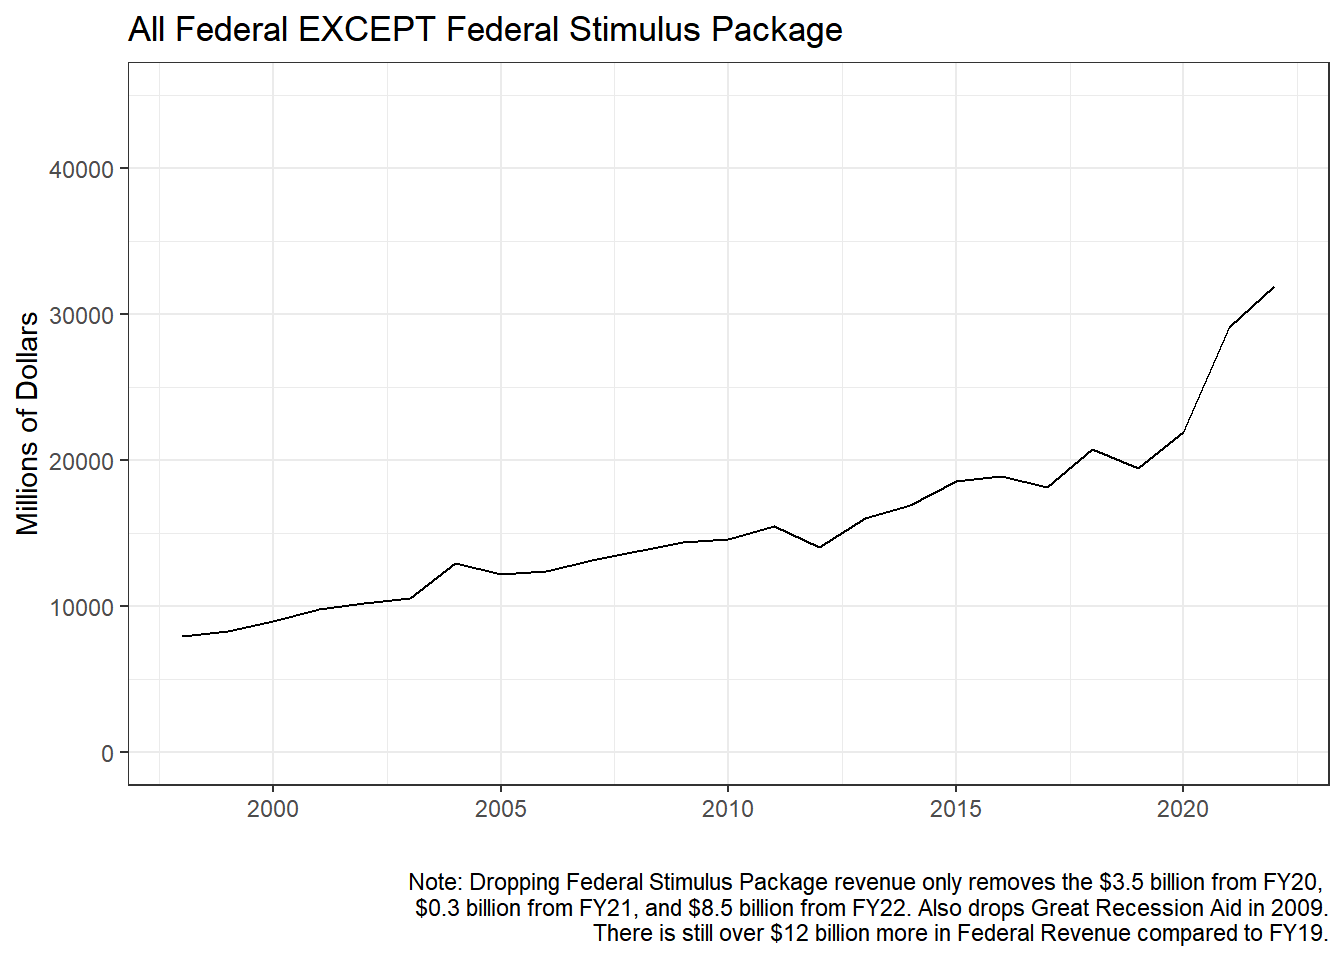
\includegraphics{./FedMoneyReceived_files/figure-pdf/unnamed-chunk-2-2.pdf}

}

\end{figure}

\begin{figure}

{\centering 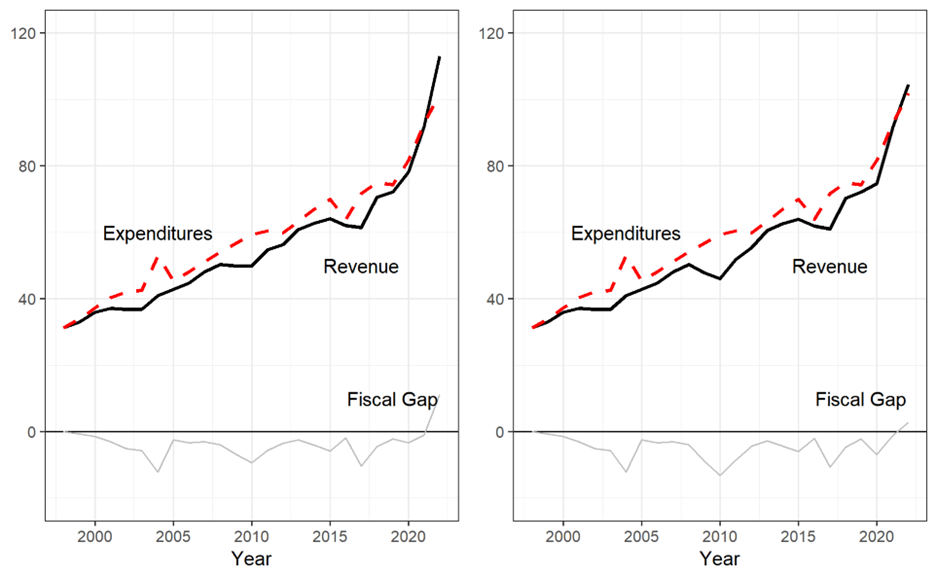
\includegraphics{./images/image-1706772717.png}

}

\caption{\label{fig-with-without-cure}With and Without State CURE Funds
from Federal Stimulus Packages}

\end{figure}

\begin{Shaded}
\begin{Highlighting}[]
\NormalTok{fedrev }\SpecialCharTok{\%\textgreater{}\%} 
  \FunctionTok{filter}\NormalTok{(fy}\SpecialCharTok{\textgreater{}}\DecValTok{2018}\NormalTok{) }\SpecialCharTok{\%\textgreater{}\%} \CommentTok{\# all fed rev after 2018 summed by year}
  \FunctionTok{group\_by}\NormalTok{(fy) }\SpecialCharTok{\%\textgreater{}\%} 
  \FunctionTok{summarize}\NormalTok{(}\AttributeTok{Revenue =} \FunctionTok{sum}\NormalTok{(receipts))}
\end{Highlighting}
\end{Shaded}

\begin{verbatim}
# A tibble: 4 x 2
     fy      Revenue
  <dbl>        <dbl>
1  2019 19473281956.
2  2020 25422362326.
3  2021 29303090912.
4  2022 40729291003.
\end{verbatim}

\begin{Shaded}
\begin{Highlighting}[]
\NormalTok{fedrev }\SpecialCharTok{\%\textgreater{}\%} 
  \FunctionTok{filter}\NormalTok{(fy}\SpecialCharTok{\textgreater{}}\DecValTok{2017}\NormalTok{) }\SpecialCharTok{\%\textgreater{}\%} \CommentTok{\# all fed rev after 2017 summed by year, \#gives precovid comparison for reference}
  \FunctionTok{group\_by}\NormalTok{(fy, rev\_type\_name) }\SpecialCharTok{\%\textgreater{}\%} 
  \FunctionTok{summarize}\NormalTok{(}\AttributeTok{Revenue =} \FunctionTok{sum}\NormalTok{(receipts))}\SpecialCharTok{\%\textgreater{}\%}
  \FunctionTok{pivot\_wider}\NormalTok{(}\AttributeTok{names\_from =}\NormalTok{ fy, }\AttributeTok{values\_from =}\NormalTok{ Revenue)}
\end{Highlighting}
\end{Shaded}

\begin{verbatim}
# A tibble: 3 x 6
  rev_type_name                         `2018`    `2019`  `2020`  `2021`  `2022`
  <chr>                                  <dbl>     <dbl>   <dbl>   <dbl>   <dbl>
1 Federal - Other                  5887128014.   6.04e 9 9.80e 9 9.37e 9 1.99e10
2 Federal Medicaid Reimbursements 13474612103.   1.21e10 1.38e10 1.76e10 1.90e10
3 Federal Transportation           1593220145.   1.36e 9 1.78e 9 2.38e 9 1.83e 9
\end{verbatim}

\begin{Shaded}
\begin{Highlighting}[]
\NormalTok{fedrev }\SpecialCharTok{\%\textgreater{}\%} 
  \CommentTok{\#federal stimulus revenue sources after 2018}
  \CommentTok{\# this is ONLY the State CURE funds from CARES and ARPA}
  \FunctionTok{filter}\NormalTok{(source\_name\_AWM }\SpecialCharTok{==} \StringTok{"FEDERAL STIMULUS PACKAGE"} \SpecialCharTok{\&}\NormalTok{ fy}\SpecialCharTok{\textgreater{}}\DecValTok{2018}\NormalTok{) }\SpecialCharTok{\%\textgreater{}\%}
  \FunctionTok{group\_by}\NormalTok{(fy) }\SpecialCharTok{\%\textgreater{}\%} 
  \FunctionTok{summarise}\NormalTok{(}\AttributeTok{receipts =} \FunctionTok{sum}\NormalTok{(receipts, }\AttributeTok{na.rm =} \ConstantTok{TRUE}\NormalTok{)}\SpecialCharTok{/}\DecValTok{1000000}\NormalTok{)}
\end{Highlighting}
\end{Shaded}

\begin{verbatim}
# A tibble: 3 x 2
     fy receipts
  <dbl>    <dbl>
1  2020    3519.
2  2021     228.
3  2022    8856.
\end{verbatim}

\begin{Shaded}
\begin{Highlighting}[]
\NormalTok{fedrev }\SpecialCharTok{\%\textgreater{}\%} 
  \FunctionTok{filter}\NormalTok{(fy}\SpecialCharTok{\textgreater{}}\DecValTok{2018}\NormalTok{) }\SpecialCharTok{\%\textgreater{}\%}
  \FunctionTok{group\_by}\NormalTok{(fy, fund\_name) }\SpecialCharTok{\%\textgreater{}\%}  \CommentTok{\# all funds that received money}
  \FunctionTok{summarise}\NormalTok{(}\AttributeTok{receipts =} \FunctionTok{sum}\NormalTok{(receipts, }\AttributeTok{na.rm =} \ConstantTok{TRUE}\NormalTok{)}\SpecialCharTok{/}\DecValTok{1000000}\NormalTok{) }\SpecialCharTok{\%\textgreater{}\%}
  \FunctionTok{arrange}\NormalTok{(}\SpecialCharTok{{-}}\NormalTok{receipts) }\SpecialCharTok{\%\textgreater{}\%}
  \FunctionTok{pivot\_wider}\NormalTok{(}\AttributeTok{names\_from =}\NormalTok{ fy, }\AttributeTok{values\_from =}\NormalTok{ receipts)}
\end{Highlighting}
\end{Shaded}

\begin{verbatim}
# A tibble: 170 x 5
   fund_name                      `2022` `2021` `2020` `2019`
   <chr>                           <dbl>  <dbl>  <dbl>  <dbl>
 1 STATE CURE                      8485.   228.    NA     NA 
 2 HEALTHCARE PROVIDER RELIEF      8450.  7551.  6007.  4033.
 3 GENERAL REVENUE                 4445.  4323.  3529.  3531.
 4 DISASTER RESPONSE AND RECOVERY   267.   276.  3520.    NA 
 5 SBE FEDERAL DEPT OF EDUCATION   3364.  2259.  1484.  1456.
 6 HOSPITAL PROVIDER               2812.  2352.  2040.  1957.
 7 COUNTY PROVIDER TRUST           2133.  1986.  1364.  1275.
 8 ROAD                            1691.  1812.  1649.  1262.
 9 EMPLOYMENT & TRAINING           1281.   412.   356.   263.
10 SBE FEDERAL DEPT OF AGRI        1111.   807.   751.   782.
# ... with 160 more rows
\end{verbatim}

\begin{Shaded}
\begin{Highlighting}[]
\NormalTok{fedrev }\SpecialCharTok{\%\textgreater{}\%} 
  \FunctionTok{filter}\NormalTok{(fy}\SpecialCharTok{\textgreater{}}\DecValTok{2018}\NormalTok{) }\SpecialCharTok{\%\textgreater{}\%}
  \FunctionTok{group\_by}\NormalTok{(fy, source\_name\_AWM) }\SpecialCharTok{\%\textgreater{}\%}  \CommentTok{\# all revenue sources}
  \FunctionTok{summarise}\NormalTok{(}\AttributeTok{receipts =} \FunctionTok{sum}\NormalTok{(receipts, }\AttributeTok{na.rm =} \ConstantTok{TRUE}\NormalTok{)}\SpecialCharTok{/}\DecValTok{1000000}\NormalTok{) }\SpecialCharTok{\%\textgreater{}\%}
  \FunctionTok{arrange}\NormalTok{(}\SpecialCharTok{{-}}\NormalTok{receipts) }\SpecialCharTok{\%\textgreater{}\%}
  \FunctionTok{pivot\_wider}\NormalTok{(}\AttributeTok{names\_from =}\NormalTok{ fy, }\AttributeTok{values\_from =}\NormalTok{ receipts)}
\end{Highlighting}
\end{Shaded}

\begin{verbatim}
# A tibble: 106 x 5
   source_name_AWM              `2022` `2021`     `2020`  `2019`
   <chr>                         <dbl>  <dbl>      <dbl>   <dbl>
 1 HEALTH AND HUMAN SERVICES   15534.  13869. 10812.     8591.  
 2 FEDERAL STIMULUS PACKAGE     8856.    228.  3519.       NA   
 3 MEDICAL ASSISTANCE           4747.   4667.  3478.     3672.  
 4 DEPARTMENT OF EDUCATION-FED  3605.   2467.  1679.     1647.  
 5 TRANSPORTATION, DEPARTMENT   1765.   2293.  1720.     1273.  
 6 AGRICULTURE, DEPARTMENT OF   1277.    963.   915.      965.  
 7 FEMA                          809.    847.    89.1       4.26
 8 CCDBG MANDATORY DISC          773.    396.   201.      148.  
 9 FED MONIES - TANF GRANT       599.    620.   621.      514.  
10 TREASURY, DEPARTMENT OF        14.8   566.     0.0996   NA   
# ... with 96 more rows
\end{verbatim}

\begin{Shaded}
\begin{Highlighting}[]
\CommentTok{\# federal transportation revenue sources}
\NormalTok{fedrev }\SpecialCharTok{\%\textgreater{}\%} 
  \FunctionTok{filter}\NormalTok{(fy}\SpecialCharTok{\textgreater{}}\DecValTok{2018}\NormalTok{, rev\_type}\SpecialCharTok{==}\StringTok{"59"}\NormalTok{) }\SpecialCharTok{\%\textgreater{}\%}
  \FunctionTok{group\_by}\NormalTok{(fy, source\_name\_AWM) }\SpecialCharTok{\%\textgreater{}\%} 
  \FunctionTok{summarise}\NormalTok{(}\AttributeTok{receipts =} \FunctionTok{sum}\NormalTok{(receipts, }\AttributeTok{na.rm =} \ConstantTok{TRUE}\NormalTok{)}\SpecialCharTok{/}\DecValTok{1000000}\NormalTok{) }\SpecialCharTok{\%\textgreater{}\%}
  \FunctionTok{arrange}\NormalTok{(}\SpecialCharTok{{-}}\NormalTok{receipts) }\SpecialCharTok{\%\textgreater{}\%}
  \FunctionTok{pivot\_wider}\NormalTok{(}\AttributeTok{names\_from =}\NormalTok{ fy, }\AttributeTok{values\_from =}\NormalTok{ receipts)}
\end{Highlighting}
\end{Shaded}

\begin{verbatim}
# A tibble: 7 x 5
  source_name_AWM               `2021`   `2022`    `2020`    `2019`
  <chr>                          <dbl>    <dbl>     <dbl>     <dbl>
1 TRANSPORTATION, DEPARTMENT  2288.    1762.    1717.     1269.    
2 URBAN MASS TRANSIT            57.4     46.7     27.1      40.4   
3 TRANSPORTATION/NHTSA          26.8     24.0     26.2      32.0   
4 TRANS/RAILROAD ADMIN           1.07     0.504   12.4      20.5   
5 IEMA-FEMA                      5.21     0.371    0.343     0.144 
6 AERONAUTICS ADMIN COST REIM    0.832    0.323    0.486     0.576 
7 US DEP OF TRANS/USEPA         NA       NA        0.0395    0.0103
\end{verbatim}

\begin{Shaded}
\begin{Highlighting}[]
\NormalTok{fedrev }\SpecialCharTok{\%\textgreater{}\%} 
  \FunctionTok{filter}\NormalTok{(fy}\SpecialCharTok{\textgreater{}}\DecValTok{2018}\NormalTok{, rev\_type}\SpecialCharTok{==}\StringTok{"58"}\NormalTok{) }\SpecialCharTok{\%\textgreater{}\%} \CommentTok{\# Fed Med only}
  \FunctionTok{group\_by}\NormalTok{(fy, source\_name\_AWM) }\SpecialCharTok{\%\textgreater{}\%} 
  \FunctionTok{summarise}\NormalTok{(}\AttributeTok{receipts =} \FunctionTok{sum}\NormalTok{(receipts, }\AttributeTok{na.rm =} \ConstantTok{TRUE}\NormalTok{)}\SpecialCharTok{/}\DecValTok{1000000}\NormalTok{) }\SpecialCharTok{\%\textgreater{}\%}
  \FunctionTok{arrange}\NormalTok{(}\SpecialCharTok{{-}}\NormalTok{receipts) }\SpecialCharTok{\%\textgreater{}\%}
  \FunctionTok{pivot\_wider}\NormalTok{(}\AttributeTok{names\_from =}\NormalTok{ fy, }\AttributeTok{values\_from =}\NormalTok{ receipts)}
\end{Highlighting}
\end{Shaded}

\begin{verbatim}
# A tibble: 6 x 5
  source_name_AWM                     `2022`      `2021`      `2020`    `2019`
  <chr>                                <dbl>       <dbl>       <dbl>     <dbl>
1 HEALTH AND HUMAN SERVICES      14290.      12877.      10053.      7835.    
2 MEDICAL ASSISTANCE              4747.       4667.       3478.      3672.    
3 HHS/HOSPITAL PARTICIPATION        NA          NA         298.       540.    
4 ENHANCED FED FIN PART-ARRA         7.87       11.5        12.8       19.5   
5 IDPH-HHS/CMS                       0.166       0.118       0.169      0.0608
6 DHHS/FFP-MEDICAID REHAB OPTION     0.00507     0.00259     0.00578    0.0128
\end{verbatim}

\begin{Shaded}
\begin{Highlighting}[]
\CommentTok{\#yearly totals for Fed Med sources above}
\NormalTok{fedrev }\SpecialCharTok{\%\textgreater{}\%} \CommentTok{\# Medicaid reimbursements and healthcare provider funds}
  \FunctionTok{filter}\NormalTok{(fy}\SpecialCharTok{\textgreater{}}\DecValTok{2018}\NormalTok{, rev\_type}\SpecialCharTok{==}\StringTok{"58"}\NormalTok{) }\SpecialCharTok{\%\textgreater{}\%}
  \FunctionTok{group\_by}\NormalTok{(fy) }\SpecialCharTok{\%\textgreater{}\%} 
  \FunctionTok{summarise}\NormalTok{(}\AttributeTok{receipts =} \FunctionTok{sum}\NormalTok{(receipts, }\AttributeTok{na.rm =} \ConstantTok{TRUE}\NormalTok{)}\SpecialCharTok{/}\DecValTok{1000000}\NormalTok{) }\SpecialCharTok{\%\textgreater{}\%}
  \FunctionTok{pivot\_wider}\NormalTok{(}\AttributeTok{names\_from =}\NormalTok{ fy, }\AttributeTok{values\_from =}\NormalTok{ receipts)}
\end{Highlighting}
\end{Shaded}

\begin{verbatim}
# A tibble: 1 x 4
  `2019` `2020` `2021` `2022`
   <dbl>  <dbl>  <dbl>  <dbl>
1 12067. 13842. 17556. 19045.
\end{verbatim}

\hypertarget{comptroller-revenue-data}{%
\section{Comptroller Revenue Data}\label{comptroller-revenue-data}}

Read the charts from the top to the bottom. Most of the graphs below
begin with either the year the money was committed or the name of the
Law that provided the funds and then shows it flowing down to either who
received the money or how it was spent.

\texttt{Sankeyattempt2022.csv} file totals \$32 billion flowing into the
state. \$3.5 came in FY20, \$12.6 billion came in FY21 and \$16.1
billion in FY22. These values include both the State CURE and other
federal grants to state departments for education, health providers, and
much more. These observations are based more on the IOC revenue data for
revenue received.

Note: \$57 million in Federal Transportation dollars are grouped with
the billions of other federal revenue for simplified graphs and
summaries.

PPP \& Health Care Enhancement act contributed to \$2.778 billion for
Provider Relief Fund. This is considered within the Medicare category in
both revenues and expenditures.

Families First Act: \$4.469 billion for Medicaid (from Health and Human
Services and deposited into Healthcare Provider Relief fund; Data Source
IOC revenue data). This fund-revenue source combo grew from \$4 billion
in 2019, \$6 billion in 2020, \$7.5 billion in 2021 and \$8.4 billion
2022.

CARES \& ESSER impacts: Revenue from source ``Department of
Education-Fed'' and deposited into ``SBE Federal Dept of Education''.
Was \$1.45 billion in 2019 and 2020 and grew to \$2.26 billion in 2021
and \$3.35 billion in 2022.

\begin{tcolorbox}[enhanced jigsaw, coltitle=black, titlerule=0mm, leftrule=.75mm, colbacktitle=quarto-callout-note-color!10!white, arc=.35mm, rightrule=.15mm, opacityback=0, colframe=quarto-callout-note-color-frame, toptitle=1mm, opacitybacktitle=0.6, bottomtitle=1mm, title=\textcolor{quarto-callout-note-color}{\faInfo}\hspace{0.5em}{Note}, colback=white, breakable, toprule=.15mm, left=2mm, bottomrule=.15mm]

\emph{Variable names in the sankeyattempt2022 file do not have the most
useful names due to the information within morphing over time as I
figured out the format to necessary for making the graphs. Any variable
names used while making these graphs might not actually contain the data
one would expect given the variable names. I do intend on renaming the
file and changing the variable names and code to something more
intuitive but have not had time to complete that task.}

\end{tcolorbox}

According to \href{covidmoneytracker.org}{federal data publicly
available}, \$52 billion has been committed to Illinois (including local
governments) but \$32 billion has been received by the state at the end
of Fiscal Year 2022 (as of June 30, 2022, excluding local governments).
An additional \$8.86 billion was committed straight to local
governments. More money has been received in FY23 but is not focused on
in this analysis. To see a graph of federal funds committed to the
State, jump to Section~\ref{sec-covid-money-tracker}.

\begin{figure}

{\centering 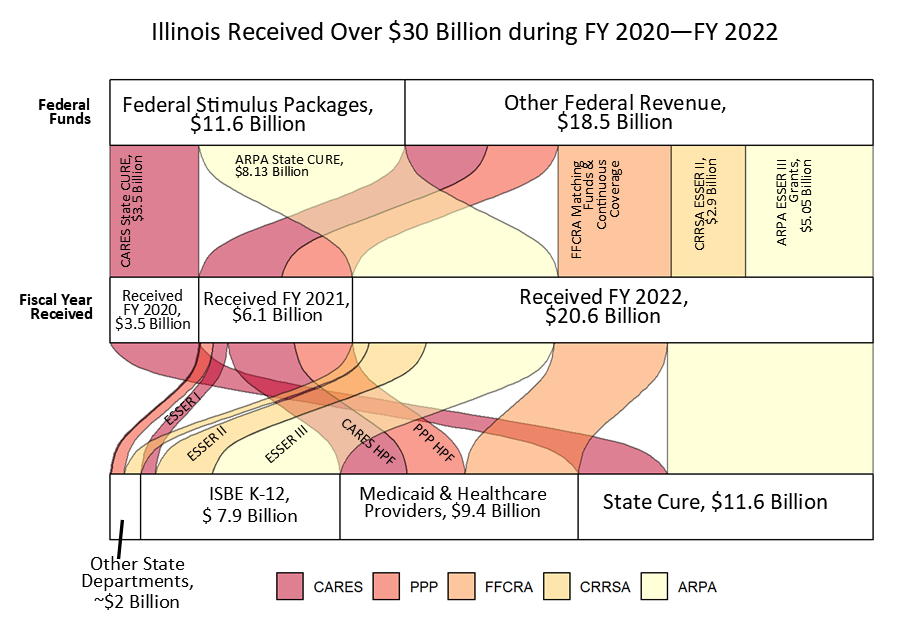
\includegraphics{./images/federal-covid-revenues.png}

}

\caption{\label{fig-rev-to-illinois}COVID-related legislation and
federal revenue into Illinois}

\end{figure}

\begin{figure}

{\centering 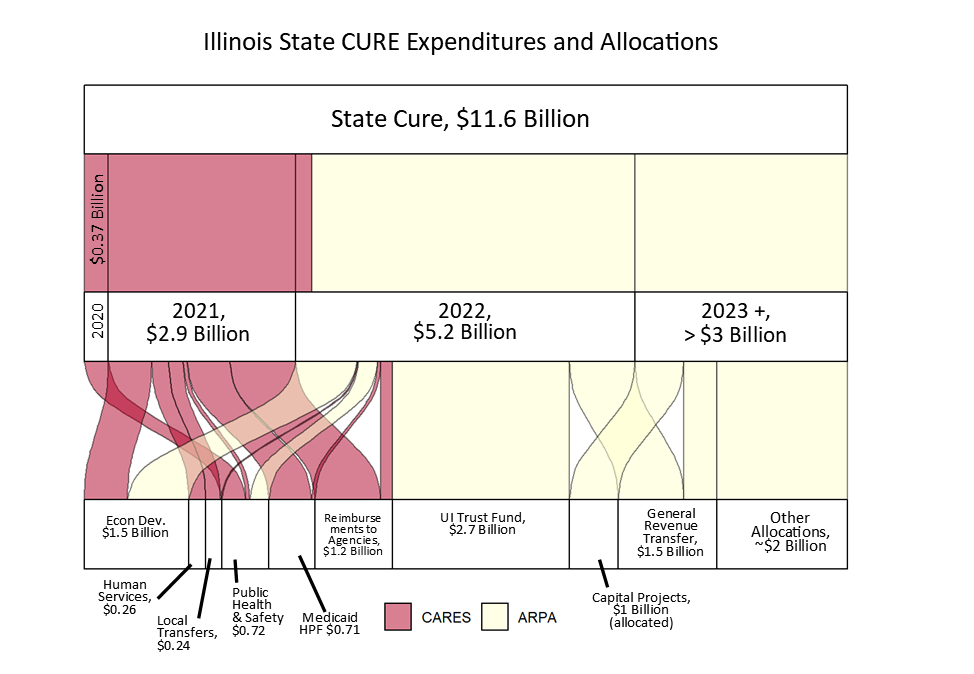
\includegraphics{./images/cure-expenditures.png}

}

\caption{\label{fig-stateCURE-expenditures}Illinois Expenditures and
Allocations for \$11.6 Billion in State CURE funds}

\end{figure}

\begin{quote}
Images below are wrong (Transportation is wrong and should be
essentially dropped, FFCRA received year is wrong. \$30 billion in
federal funds.)
\end{quote}

\begin{figure}

{\centering 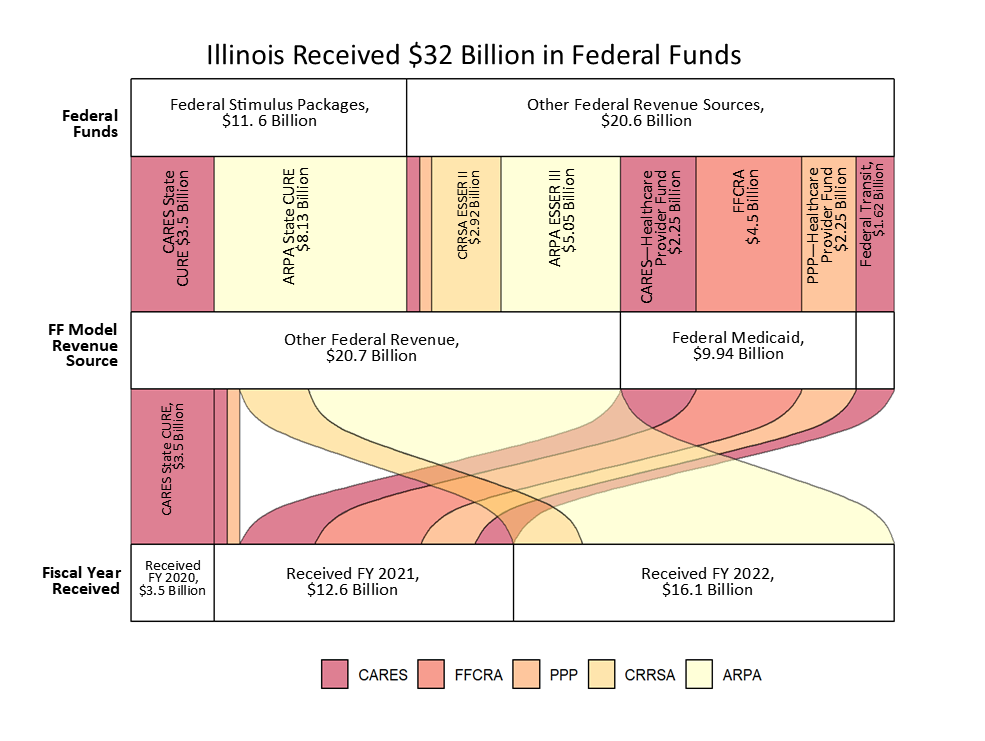
\includegraphics[width=4.83333in,height=\textheight]{./images/revenues_ioc_32bil_byyear-02.png}

}

\caption{\label{fig-ioc_received_32bil_byyear}The image above shows the
federal revenue type, the year it was received, and type of federal
revenue source that the funds fall within using the Fiscal Futures
methodology.}

\end{figure}

\begin{figure}

{\centering 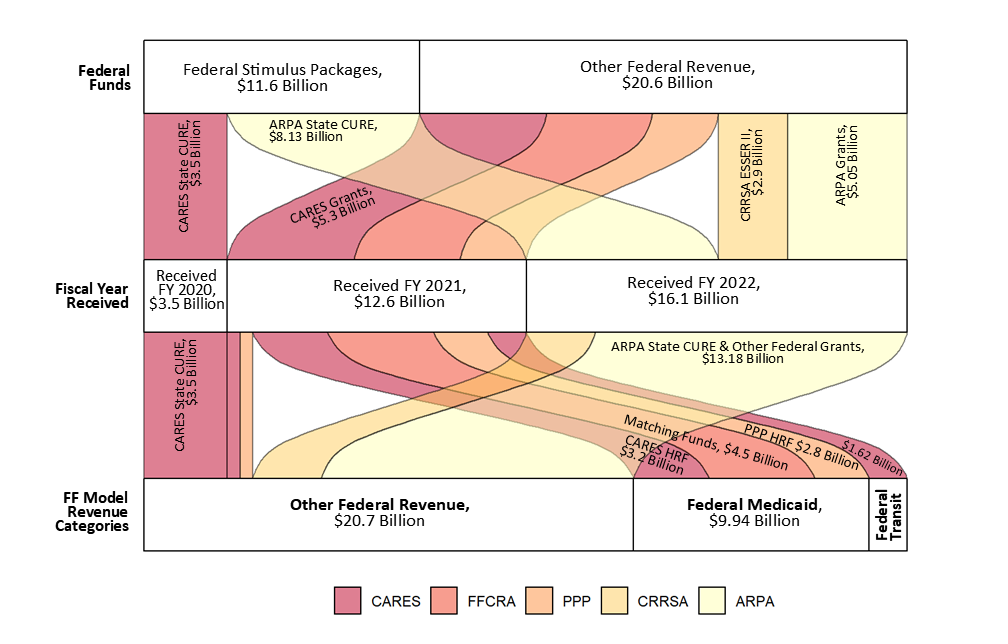
\includegraphics[width=4.16667in,height=\textheight]{./images/revenues_ioc_32bil_byrevsource.png}

}

\caption{\label{fig-received-ioc32bil-byrevsource}The image above shows
the federal revenue type (State CURE or other), the year it was
received, and the revenue source category it falls under using the
Fiscal Futures methodology. It contains the same information as the
chart above but the Year and Source type are flipped.}

\end{figure}

\begin{Shaded}
\begin{Highlighting}[]
\NormalTok{sankey\_rev\_ioc }\OtherTok{\textless{}{-}} \FunctionTok{read\_csv}\NormalTok{(}\StringTok{"sankeyattempt2022.csv"}\NormalTok{) }\SpecialCharTok{\%\textgreater{}\%} 
  \FunctionTok{filter}\NormalTok{(StFund }\SpecialCharTok{==} \StringTok{"Total"}\NormalTok{)}


\FunctionTok{brewer.pal}\NormalTok{(}\AttributeTok{n =} \DecValTok{8}\NormalTok{, }\AttributeTok{name =} \StringTok{\textquotesingle{}YlOrRd\textquotesingle{}}\NormalTok{)}
\end{Highlighting}
\end{Shaded}

\begin{verbatim}
[1] "#FFFFCC" "#FFEDA0" "#FED976" "#FEB24C" "#FD8D3C" "#FC4E2A" "#E31A1C"
[8] "#B10026"
\end{verbatim}

\begin{Shaded}
\begin{Highlighting}[]
\NormalTok{sankey\_rev\_ioc }\OtherTok{\textless{}{-}}\NormalTok{ sankey\_rev\_ioc }\SpecialCharTok{\%\textgreater{}\%} \FunctionTok{select}\NormalTok{(Federal, FF\_Cat, StateFunds, StFund, Expenditures, value, Notes, Notes2, stfundname) }\SpecialCharTok{\%\textgreater{}\%}
  \FunctionTok{filter}\NormalTok{(StFund }\SpecialCharTok{==} \StringTok{"Total"}\NormalTok{) }\SpecialCharTok{\%\textgreater{}\%}
  \FunctionTok{mutate}\NormalTok{(}\AttributeTok{value=}\FunctionTok{as.numeric}\NormalTok{(value),}
         \CommentTok{\# keeps order of year received from oldest to newest in graphs}
    \AttributeTok{StateFunds =} \FunctionTok{factor}\NormalTok{(StateFunds, }\AttributeTok{levels =} \FunctionTok{c}\NormalTok{(}\StringTok{"Total\_received\_fy20"}\NormalTok{,}\StringTok{"Total\_received\_fy21"}\NormalTok{, }\StringTok{"Total\_received\_fy22"}\NormalTok{)),}
    \CommentTok{\# other includes transit and public health grants}
                 \AttributeTok{Expenditures\_ordered =} \FunctionTok{factor}\NormalTok{(Expenditures, }\AttributeTok{levels =} \FunctionTok{c}\NormalTok{(}\StringTok{"Federal Other"}\NormalTok{, }\StringTok{"Other"}\NormalTok{,  }\StringTok{"K{-}12"}\NormalTok{,  }\StringTok{"Medicaid"}\NormalTok{, }\StringTok{"Medicare"}\NormalTok{, }\StringTok{"Misc."}\NormalTok{)),}
    \AttributeTok{FF\_Cat\_ordered=}\FunctionTok{factor}\NormalTok{(FF\_Cat, }\AttributeTok{levels =} \FunctionTok{c}\NormalTok{(}\StringTok{"Other"}\NormalTok{, }\StringTok{"Transit"}\NormalTok{, }\StringTok{"Medicare"}\NormalTok{,}\StringTok{"Medicaid"}\NormalTok{, }\StringTok{"Federal Other"}\NormalTok{)),}
    \AttributeTok{Federal\_ordered =} \FunctionTok{factor}\NormalTok{(Federal, }\AttributeTok{levels =} \StringTok{"Medicaid"}\NormalTok{, }\StringTok{"Medicare"}\NormalTok{, }\StringTok{"Federal Other"}\NormalTok{),}
    \CommentTok{\# keeps Legislation in chronological order,}
    \CommentTok{\# groups FFRCA and PPP legislation into Other *, helps simplify some graphs }
         \AttributeTok{Notes2 =} \FunctionTok{factor}\NormalTok{(Notes2, }\AttributeTok{levels =} \FunctionTok{c}\NormalTok{(}\StringTok{"CARES"}\NormalTok{, }\StringTok{"Other *"}\NormalTok{, }\StringTok{"CRRSA"}\NormalTok{, }\StringTok{"ARPA"}\NormalTok{)),}
        \CommentTok{\# keeps legislation in chronological order}
         \AttributeTok{Notes =} \FunctionTok{factor}\NormalTok{(Notes, }\AttributeTok{levels =} \FunctionTok{c}\NormalTok{(}\StringTok{"CARES"}\NormalTok{,  }\StringTok{"PPP"}\NormalTok{, }\StringTok{"FFCRA"}\NormalTok{,}\StringTok{"CRRSA"}\NormalTok{, }\StringTok{"ARPA"}\NormalTok{)))}

\NormalTok{sankey\_rev\_ioc }\SpecialCharTok{\%\textgreater{}\%} \FunctionTok{filter}\NormalTok{( Federal }\SpecialCharTok{==} \StringTok{"Federal Stimulus Packages"}\NormalTok{) }\SpecialCharTok{\%\textgreater{}\%}
\FunctionTok{ggplot}\NormalTok{( }
       \FunctionTok{aes}\NormalTok{(}\AttributeTok{y =}\NormalTok{ value, }
            \AttributeTok{axis3=}\NormalTok{FF\_Cat, }\AttributeTok{axis2=}\NormalTok{Expenditures, }\AttributeTok{axis1 =}\NormalTok{ StateFunds, }\AttributeTok{label =} \StringTok{"stratum"}\NormalTok{)) }\SpecialCharTok{+}
  \FunctionTok{geom\_flow}\NormalTok{(}\FunctionTok{aes}\NormalTok{(}\AttributeTok{fill =}\NormalTok{ Notes), }\AttributeTok{color =} \StringTok{"black"}\NormalTok{, }\AttributeTok{reverse=}\ConstantTok{FALSE}\NormalTok{) }\SpecialCharTok{+}
  \FunctionTok{geom\_stratum}\NormalTok{(}\AttributeTok{reverse=}\ConstantTok{FALSE}\NormalTok{)}\SpecialCharTok{+}
\FunctionTok{coord\_flip}\NormalTok{()}\SpecialCharTok{+}
   \FunctionTok{scale\_fill\_brewer}\NormalTok{(}\AttributeTok{palette =} \StringTok{"YlOrRd"}\NormalTok{, }\AttributeTok{direction =} \SpecialCharTok{{-}}\DecValTok{1}\NormalTok{)}\SpecialCharTok{+}
  \FunctionTok{theme\_void}\NormalTok{() }\SpecialCharTok{+}
  \FunctionTok{theme}\NormalTok{(}\AttributeTok{legend.position =} \StringTok{"bottom"}\NormalTok{) }\SpecialCharTok{+} 
      \FunctionTok{geom\_text}\NormalTok{(}\AttributeTok{stat =} \StringTok{"stratum"}\NormalTok{, }\FunctionTok{aes}\NormalTok{(}\AttributeTok{label =} \FunctionTok{after\_stat}\NormalTok{(stratum)), }\AttributeTok{size =} \DecValTok{2}\NormalTok{, }\AttributeTok{reverse=}\ConstantTok{FALSE}\NormalTok{)}\SpecialCharTok{+}
  \FunctionTok{labs}\NormalTok{(}\AttributeTok{title =} \StringTok{"Over $8 billion in FY22, $11.6 Billion in State CURE total"}\NormalTok{)}
\end{Highlighting}
\end{Shaded}

\begin{figure}[H]

{\centering \includegraphics{./FedMoneyReceived_files/figure-pdf/unnamed-chunk-4-1.pdf}

}

\end{figure}

\begin{Shaded}
\begin{Highlighting}[]
\FunctionTok{ggplot}\NormalTok{(sankey\_rev\_ioc, }
       \FunctionTok{aes}\NormalTok{(}\AttributeTok{y =}\NormalTok{ value, }
           \AttributeTok{axis4 =}\NormalTok{ Federal, }\AttributeTok{axis3=}\NormalTok{FF\_Cat, }\AttributeTok{axis2=}\NormalTok{Expenditures, }\AttributeTok{axis1 =}\NormalTok{ StateFunds, }\AttributeTok{label =} \StringTok{"stratum"}\NormalTok{)) }\SpecialCharTok{+}
  \FunctionTok{geom\_flow}\NormalTok{(}\FunctionTok{aes}\NormalTok{(}\AttributeTok{fill =}\NormalTok{ Notes), }\AttributeTok{color =} \StringTok{"black"}\NormalTok{, }\AttributeTok{reverse=}\ConstantTok{FALSE}\NormalTok{) }\SpecialCharTok{+}
  \FunctionTok{geom\_stratum}\NormalTok{(}\AttributeTok{reverse=}\ConstantTok{FALSE}\NormalTok{)}\SpecialCharTok{+}
\FunctionTok{coord\_flip}\NormalTok{()}\SpecialCharTok{+}
   \FunctionTok{scale\_fill\_brewer}\NormalTok{(}\AttributeTok{palette =} \StringTok{"YlOrRd"}\NormalTok{, }\AttributeTok{direction =} \SpecialCharTok{{-}}\DecValTok{1}\NormalTok{)}\SpecialCharTok{+}
  \FunctionTok{theme\_void}\NormalTok{() }\SpecialCharTok{+}
  \FunctionTok{theme}\NormalTok{(}\AttributeTok{legend.position =} \StringTok{"bottom"}\NormalTok{) }\SpecialCharTok{+} 
      \FunctionTok{geom\_text}\NormalTok{(}\AttributeTok{stat =} \StringTok{"stratum"}\NormalTok{, }\FunctionTok{aes}\NormalTok{(}\AttributeTok{label =} \FunctionTok{after\_stat}\NormalTok{(stratum)), }\AttributeTok{size =} \DecValTok{2}\NormalTok{, }\AttributeTok{reverse=}\ConstantTok{FALSE}\NormalTok{)}\SpecialCharTok{+}
  \FunctionTok{labs}\NormalTok{(}\AttributeTok{title =} \StringTok{"$30.6 billion recieved FY20{-}FY22"}\NormalTok{)}
\end{Highlighting}
\end{Shaded}

\begin{figure}[H]

{\centering 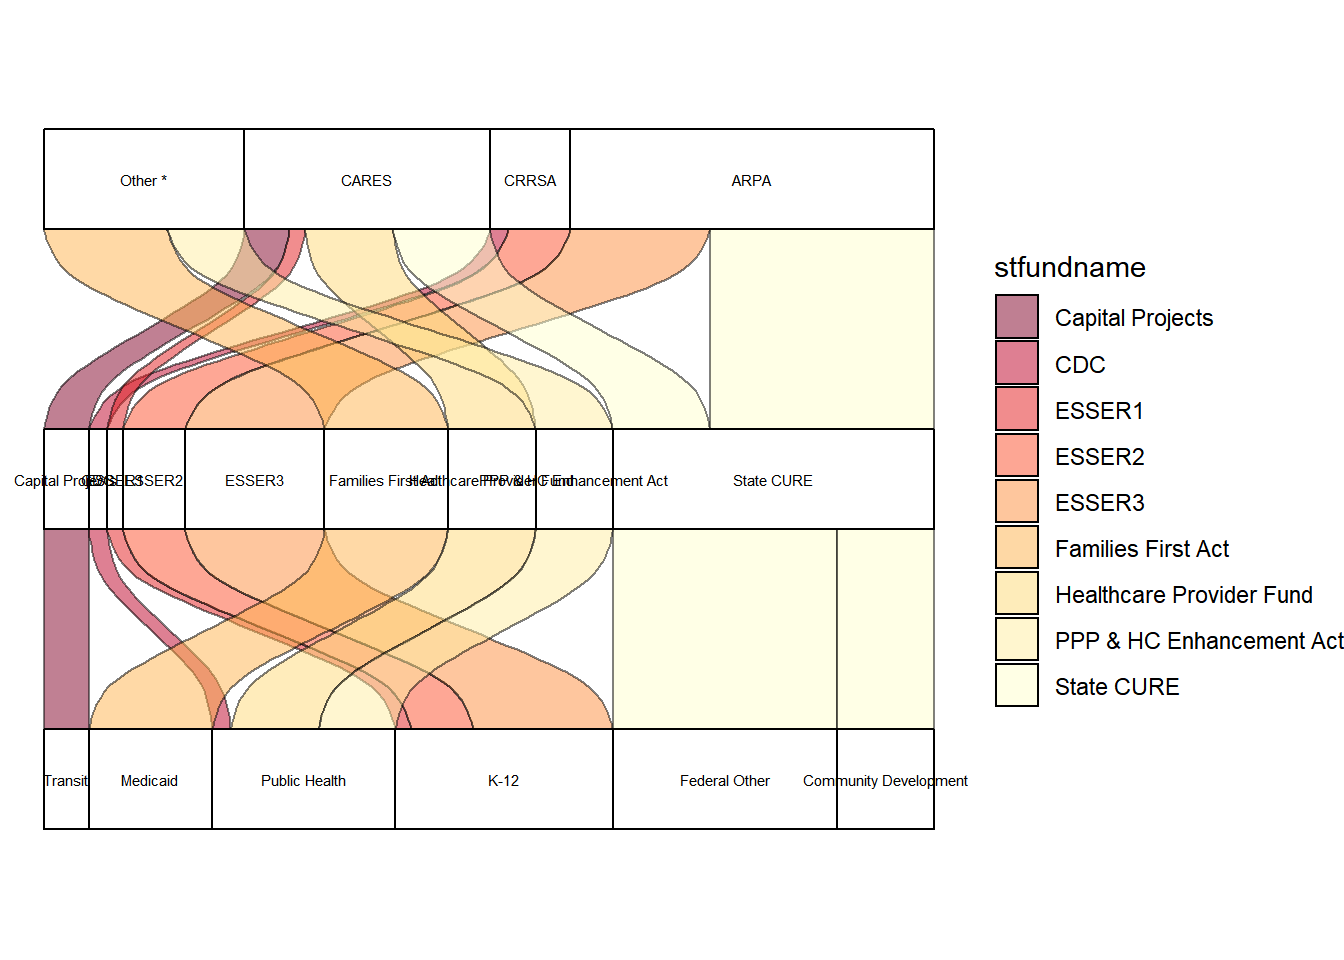
\includegraphics{./FedMoneyReceived_files/figure-pdf/unnamed-chunk-4-2.pdf}

}

\end{figure}

\begin{Shaded}
\begin{Highlighting}[]
\FunctionTok{ggplot}\NormalTok{(sankey\_rev\_ioc, }
       \FunctionTok{aes}\NormalTok{(}\AttributeTok{y =}\NormalTok{ value, }
           \AttributeTok{axis3 =}\NormalTok{ Federal, }\AttributeTok{axis2 =}\NormalTok{ StateFunds, }\AttributeTok{axis1=}\NormalTok{Expenditures, }\AttributeTok{label =} \StringTok{"stratum"}\NormalTok{)) }\SpecialCharTok{+}
  \FunctionTok{geom\_flow}\NormalTok{(}\FunctionTok{aes}\NormalTok{(}\AttributeTok{fill =}\NormalTok{ Notes), }\AttributeTok{color =} \StringTok{"black"}\NormalTok{, }\AttributeTok{reverse=}\ConstantTok{FALSE}\NormalTok{) }\SpecialCharTok{+}
  \FunctionTok{geom\_stratum}\NormalTok{(}\AttributeTok{reverse=}\ConstantTok{FALSE}\NormalTok{)}\SpecialCharTok{+}
\FunctionTok{coord\_flip}\NormalTok{()}\SpecialCharTok{+}
   \FunctionTok{scale\_fill\_brewer}\NormalTok{(}\AttributeTok{palette =} \StringTok{"YlOrRd"}\NormalTok{, }\AttributeTok{direction =} \SpecialCharTok{{-}}\DecValTok{1}\NormalTok{)}\SpecialCharTok{+}
  \FunctionTok{theme\_void}\NormalTok{() }\SpecialCharTok{+}
  \FunctionTok{theme}\NormalTok{(}\AttributeTok{legend.position =} \StringTok{"bottom"}\NormalTok{, }\AttributeTok{legend.title =} \FunctionTok{element\_blank}\NormalTok{()) }\SpecialCharTok{+} 
      \FunctionTok{geom\_text}\NormalTok{(}\AttributeTok{stat =} \StringTok{"stratum"}\NormalTok{, }\FunctionTok{aes}\NormalTok{(}\AttributeTok{label =} \FunctionTok{after\_stat}\NormalTok{(stratum)), }\AttributeTok{size =} \DecValTok{2}\NormalTok{, }\AttributeTok{reverse=}\ConstantTok{FALSE}\NormalTok{)}\SpecialCharTok{+}
  \FunctionTok{labs}\NormalTok{(}\AttributeTok{title =} \StringTok{"$30.6 billion in federal aid recieved by Illinois FY20{-}FY22"}\NormalTok{,}
       \AttributeTok{subtitle =} \StringTok{"$11.6 Billion for State CURE"}\NormalTok{)}
\end{Highlighting}
\end{Shaded}

\begin{figure}[H]

{\centering 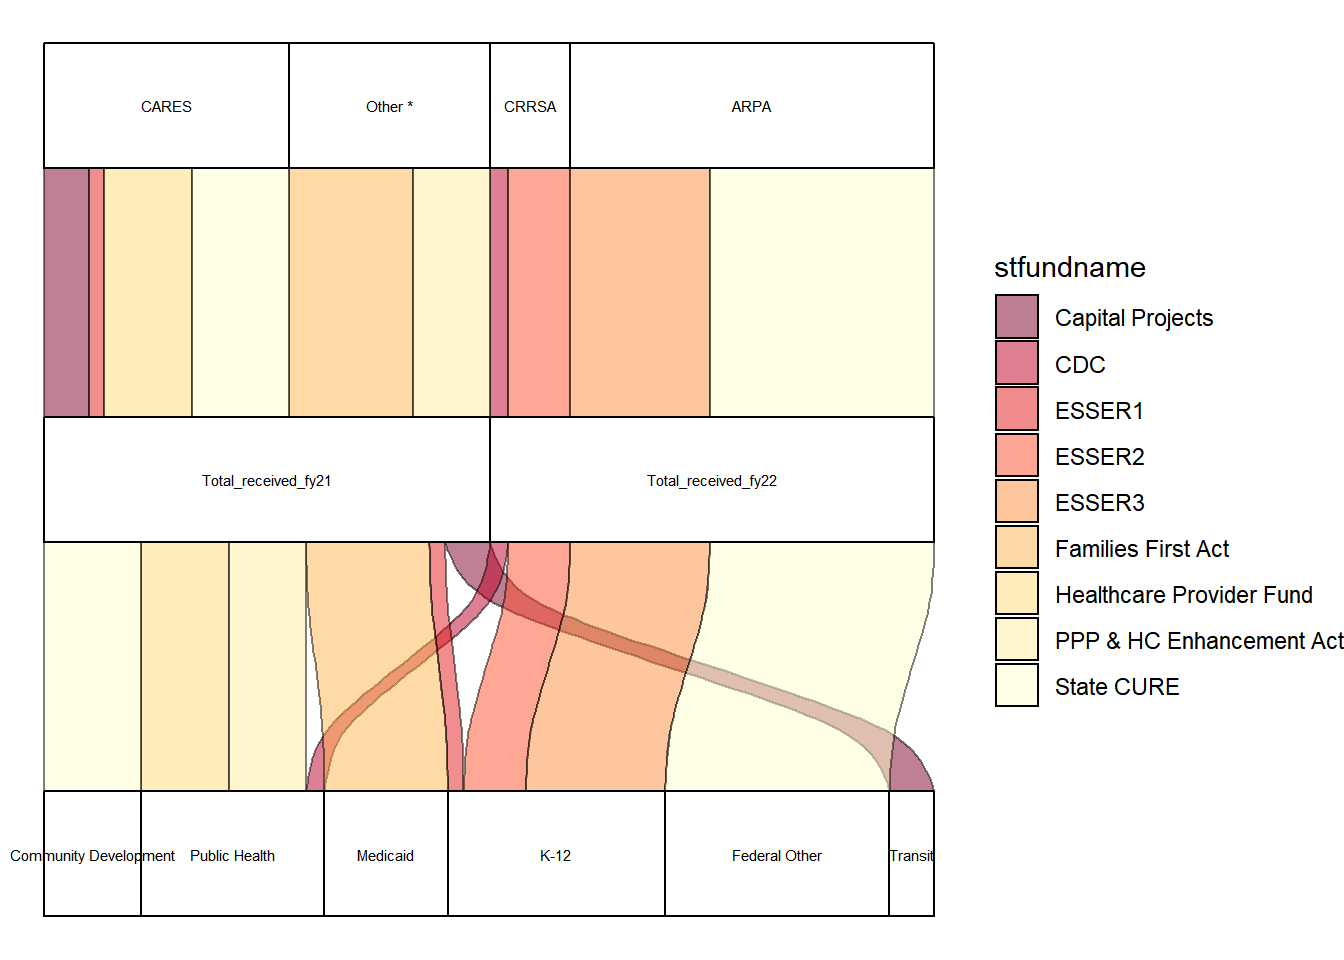
\includegraphics{./FedMoneyReceived_files/figure-pdf/unnamed-chunk-4-3.pdf}

}

\end{figure}

\begin{Shaded}
\begin{Highlighting}[]
\FunctionTok{ggplot}\NormalTok{(sankey\_rev\_ioc, }
       \FunctionTok{aes}\NormalTok{(}\AttributeTok{y =}\NormalTok{ value, }
           \AttributeTok{axis3 =}\NormalTok{ Notes, }\AttributeTok{axis2 =}\NormalTok{ StateFunds, }\AttributeTok{axis1=}\NormalTok{Expenditures, }\AttributeTok{label =} \StringTok{"stratum"}\NormalTok{)) }\SpecialCharTok{+}
  \FunctionTok{geom\_flow}\NormalTok{(}\FunctionTok{aes}\NormalTok{(}\AttributeTok{fill =}\NormalTok{ Federal), }\AttributeTok{color =} \StringTok{"black"}\NormalTok{, }\AttributeTok{reverse=}\ConstantTok{FALSE}\NormalTok{) }\SpecialCharTok{+}
  \FunctionTok{geom\_stratum}\NormalTok{(}\AttributeTok{reverse=}\ConstantTok{FALSE}\NormalTok{)}\SpecialCharTok{+}
\FunctionTok{coord\_flip}\NormalTok{()}\SpecialCharTok{+}
   \FunctionTok{scale\_fill\_brewer}\NormalTok{(}\AttributeTok{palette =} \StringTok{"YlOrRd"}\NormalTok{, }\AttributeTok{direction =} \SpecialCharTok{{-}}\DecValTok{1}\NormalTok{)}\SpecialCharTok{+}
  \FunctionTok{theme\_void}\NormalTok{() }\SpecialCharTok{+}
  \FunctionTok{theme}\NormalTok{(}\AttributeTok{legend.position =} \StringTok{"bottom"}\NormalTok{, }\AttributeTok{legend.title =} \FunctionTok{element\_blank}\NormalTok{()) }\SpecialCharTok{+} 
      \FunctionTok{geom\_text}\NormalTok{(}\AttributeTok{stat =} \StringTok{"stratum"}\NormalTok{, }\FunctionTok{aes}\NormalTok{(}\AttributeTok{label =} \FunctionTok{after\_stat}\NormalTok{(stratum)), }\AttributeTok{size =} \DecValTok{2}\NormalTok{, }\AttributeTok{reverse=}\ConstantTok{FALSE}\NormalTok{)}\SpecialCharTok{+}
  \FunctionTok{labs}\NormalTok{(}\AttributeTok{title =} \StringTok{"$30.6 billion in federal aid recieved by Illinois FY20{-}FY22"}\NormalTok{,}
       \AttributeTok{subtitle =} \StringTok{"$11.6 Billion for State CURE"}\NormalTok{)}
\end{Highlighting}
\end{Shaded}

\begin{figure}[H]

{\centering 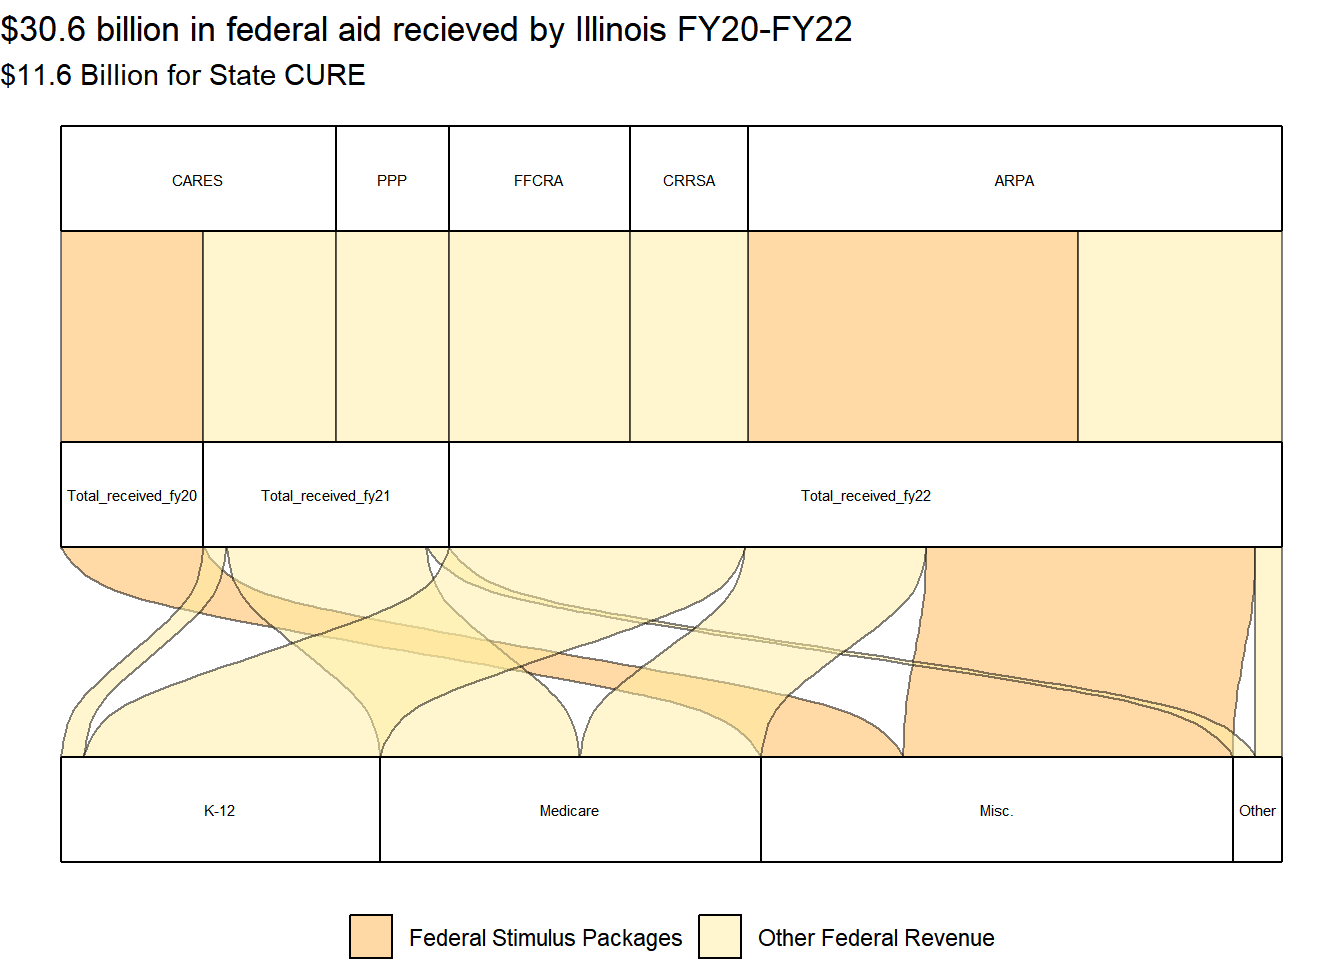
\includegraphics{./FedMoneyReceived_files/figure-pdf/unnamed-chunk-4-4.pdf}

}

\end{figure}

\begin{Shaded}
\begin{Highlighting}[]
\FunctionTok{ggplot}\NormalTok{(sankey\_rev\_ioc, }
       \FunctionTok{aes}\NormalTok{(}\AttributeTok{y =}\NormalTok{ value, }
           \AttributeTok{axis3 =}\NormalTok{ Notes, }\AttributeTok{axis1 =}\NormalTok{ StateFunds, }\AttributeTok{axis2=}\NormalTok{Expenditures, }\AttributeTok{label =} \StringTok{"stratum"}\NormalTok{)) }\SpecialCharTok{+}
  \FunctionTok{geom\_flow}\NormalTok{(}\FunctionTok{aes}\NormalTok{(}\AttributeTok{fill =}\NormalTok{ Federal), }\AttributeTok{color =} \StringTok{"black"}\NormalTok{, }\AttributeTok{reverse=}\ConstantTok{FALSE}\NormalTok{) }\SpecialCharTok{+}
  \FunctionTok{geom\_stratum}\NormalTok{(}\AttributeTok{reverse=}\ConstantTok{FALSE}\NormalTok{)}\SpecialCharTok{+}
\FunctionTok{coord\_flip}\NormalTok{()}\SpecialCharTok{+}
   \FunctionTok{scale\_fill\_brewer}\NormalTok{(}\AttributeTok{palette =} \StringTok{"YlOrRd"}\NormalTok{, }\AttributeTok{direction =} \SpecialCharTok{{-}}\DecValTok{1}\NormalTok{)}\SpecialCharTok{+}
  \FunctionTok{theme\_void}\NormalTok{() }\SpecialCharTok{+}
  \FunctionTok{theme}\NormalTok{(}\AttributeTok{legend.position =} \StringTok{"bottom"}\NormalTok{, }\AttributeTok{legend.title =} \FunctionTok{element\_blank}\NormalTok{()) }\SpecialCharTok{+} 
      \FunctionTok{geom\_text}\NormalTok{(}\AttributeTok{stat =} \StringTok{"stratum"}\NormalTok{, }\FunctionTok{aes}\NormalTok{(}\AttributeTok{label =} \FunctionTok{after\_stat}\NormalTok{(stratum)), }\AttributeTok{size =} \DecValTok{2}\NormalTok{, }\AttributeTok{reverse=}\ConstantTok{FALSE}\NormalTok{)}\SpecialCharTok{+}
  \FunctionTok{labs}\NormalTok{(}\AttributeTok{title =} \StringTok{"$30.6 billion in federal aid recieved by Illinois FY20{-}FY22"}\NormalTok{,}
       \AttributeTok{subtitle =} \StringTok{"$11.6 Billion for State CURE"}\NormalTok{)}
\end{Highlighting}
\end{Shaded}

\begin{figure}[H]

{\centering 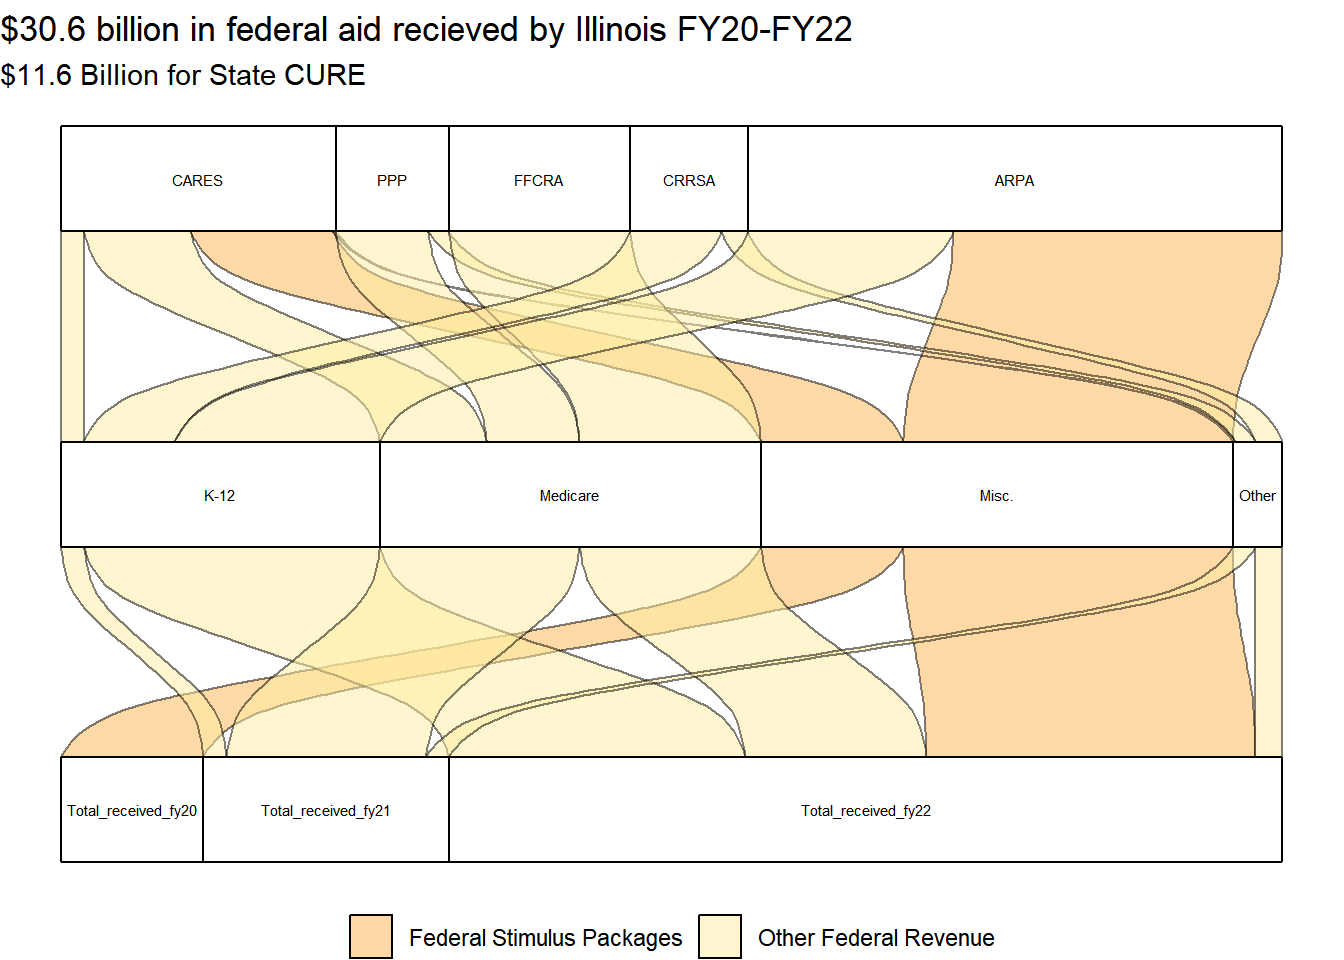
\includegraphics{./FedMoneyReceived_files/figure-pdf/unnamed-chunk-4-5.pdf}

}

\end{figure}

\begin{Shaded}
\begin{Highlighting}[]
\FunctionTok{ggplot}\NormalTok{(sankey\_rev\_ioc, }
       \FunctionTok{aes}\NormalTok{(}\AttributeTok{y =}\NormalTok{ value, }
           \AttributeTok{axis4 =}\NormalTok{ Notes, }\AttributeTok{axis2 =}\NormalTok{ StateFunds, }\AttributeTok{axis3=}\NormalTok{Expenditures, }\AttributeTok{label =} \StringTok{"stratum"}\NormalTok{)) }\SpecialCharTok{+}
  \FunctionTok{geom\_flow}\NormalTok{(}\FunctionTok{aes}\NormalTok{(}\AttributeTok{fill =}\NormalTok{ Federal), }\AttributeTok{color =} \StringTok{"black"}\NormalTok{, }\AttributeTok{reverse=}\ConstantTok{FALSE}\NormalTok{) }\SpecialCharTok{+}
  \FunctionTok{geom\_stratum}\NormalTok{(}\AttributeTok{reverse=}\ConstantTok{FALSE}\NormalTok{)}\SpecialCharTok{+}
\FunctionTok{coord\_flip}\NormalTok{()}\SpecialCharTok{+}
   \FunctionTok{scale\_fill\_brewer}\NormalTok{(}\AttributeTok{palette =} \StringTok{"YlOrRd"}\NormalTok{, }\AttributeTok{direction =} \SpecialCharTok{{-}}\DecValTok{1}\NormalTok{)}\SpecialCharTok{+}
  \FunctionTok{theme\_void}\NormalTok{() }\SpecialCharTok{+}
  \FunctionTok{theme}\NormalTok{(}\AttributeTok{legend.position =} \StringTok{"bottom"}\NormalTok{, }\AttributeTok{legend.title =} \FunctionTok{element\_blank}\NormalTok{()) }\SpecialCharTok{+} 
      \FunctionTok{geom\_text}\NormalTok{(}\AttributeTok{stat =} \StringTok{"stratum"}\NormalTok{, }\FunctionTok{aes}\NormalTok{(}\AttributeTok{label =} \FunctionTok{after\_stat}\NormalTok{(stratum)), }\AttributeTok{size =} \DecValTok{2}\NormalTok{, }\AttributeTok{reverse=}\ConstantTok{FALSE}\NormalTok{)}\SpecialCharTok{+}
  \FunctionTok{labs}\NormalTok{(}\AttributeTok{title =} \StringTok{"$30.6 billion in federal aid recieved by Illinois FY20{-}FY22"}\NormalTok{,}
       \AttributeTok{subtitle =} \StringTok{"$11.6 Billion for State CURE"}\NormalTok{)}
\end{Highlighting}
\end{Shaded}

\begin{figure}[H]

{\centering 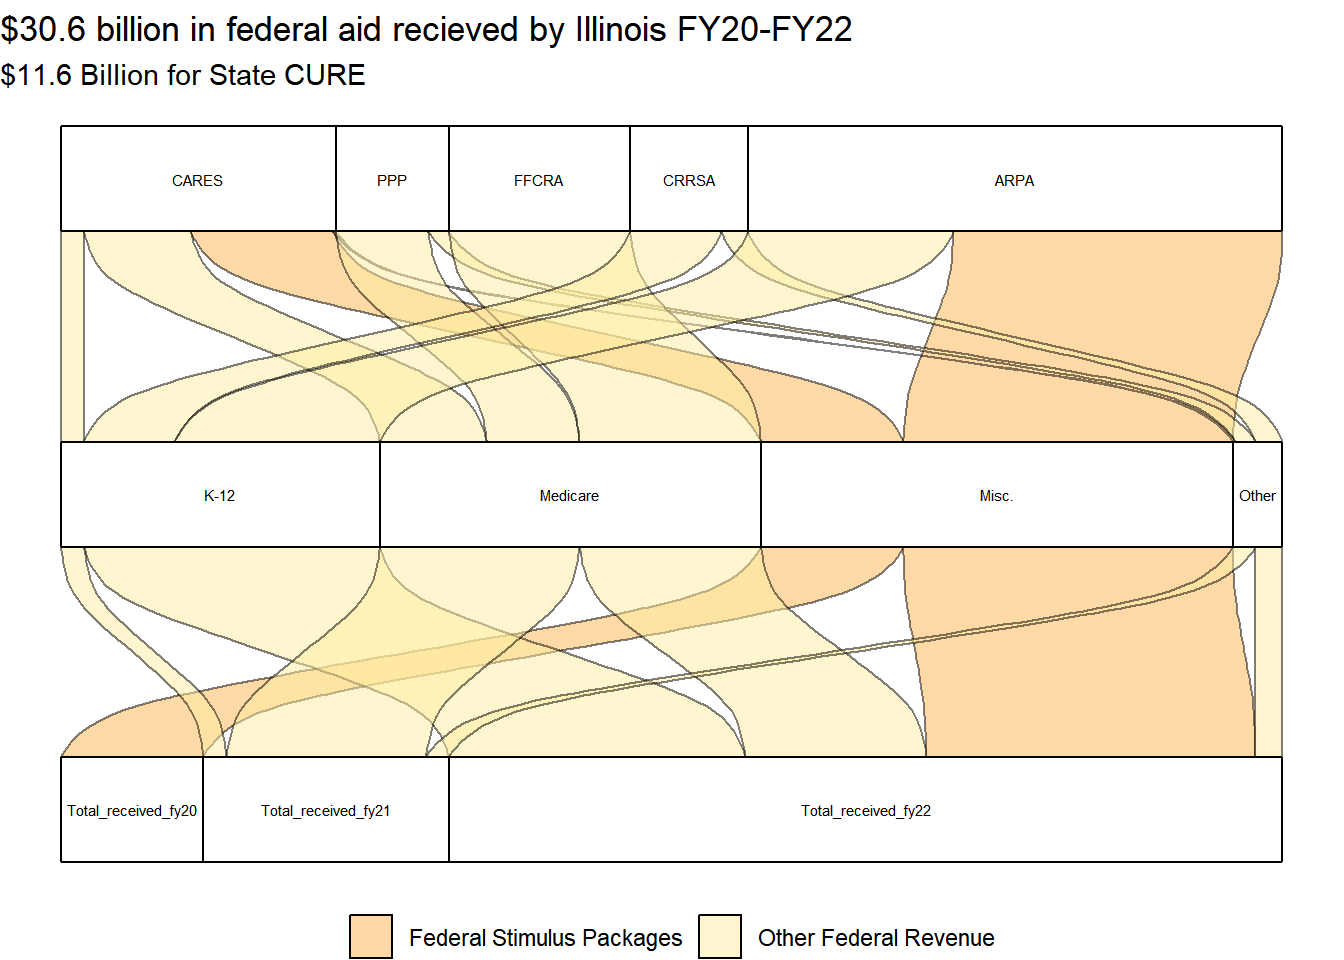
\includegraphics{./FedMoneyReceived_files/figure-pdf/unnamed-chunk-4-6.pdf}

}

\end{figure}

\begin{Shaded}
\begin{Highlighting}[]
\FunctionTok{ggplot}\NormalTok{(sankey\_rev\_ioc, }
       \FunctionTok{aes}\NormalTok{(}\AttributeTok{y =}\NormalTok{ value, }
           \AttributeTok{axis3 =}\NormalTok{ Federal,   }\AttributeTok{axis2 =}\NormalTok{ StateFunds, }\AttributeTok{axis1=}\NormalTok{Expenditures\_ordered,  }\AttributeTok{label =} \StringTok{"stratum"}\NormalTok{)) }\SpecialCharTok{+}
  \FunctionTok{geom\_flow}\NormalTok{(}\FunctionTok{aes}\NormalTok{(}\AttributeTok{fill =}\NormalTok{ Notes), }\AttributeTok{color =} \StringTok{"black"}\NormalTok{, }\AttributeTok{reverse=}\ConstantTok{FALSE}\NormalTok{) }\SpecialCharTok{+}
  \FunctionTok{geom\_stratum}\NormalTok{(}\AttributeTok{reverse=}\ConstantTok{FALSE}\NormalTok{)}\SpecialCharTok{+}
\FunctionTok{coord\_flip}\NormalTok{()}\SpecialCharTok{+}
   \FunctionTok{scale\_fill\_brewer}\NormalTok{(}\AttributeTok{palette =} \StringTok{"YlOrRd"}\NormalTok{, }\AttributeTok{direction =} \SpecialCharTok{{-}}\DecValTok{1}\NormalTok{)}\SpecialCharTok{+}
  \FunctionTok{theme\_void}\NormalTok{() }\SpecialCharTok{+}
  \FunctionTok{theme}\NormalTok{(}\AttributeTok{legend.position =} \StringTok{"bottom"}\NormalTok{, }\AttributeTok{legend.title =} \FunctionTok{element\_blank}\NormalTok{()) }\SpecialCharTok{+} 
  \FunctionTok{labs}\NormalTok{(}\AttributeTok{title =} \StringTok{"$30.6 billion in federal aid recieved by Illinois FY20{-}FY22"}\NormalTok{,}
       \AttributeTok{subtitle =} \StringTok{"$11.6 Billion for State CURE"}\NormalTok{)}
\end{Highlighting}
\end{Shaded}

\begin{figure}[H]

{\centering 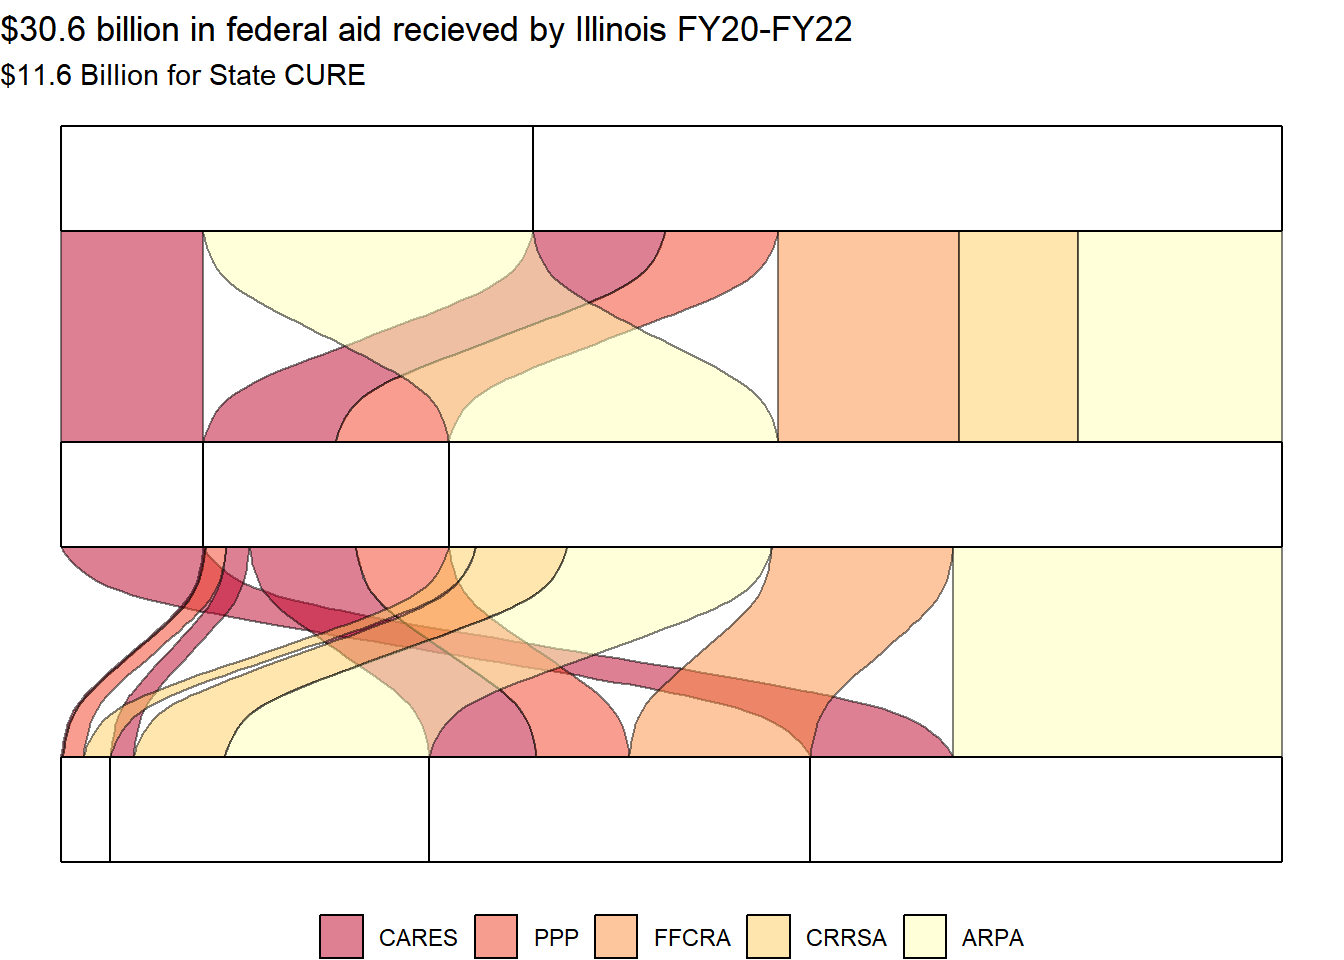
\includegraphics{./FedMoneyReceived_files/figure-pdf/unnamed-chunk-4-7.pdf}

}

\end{figure}

Some of the grouping and summarizing of data to calculate the values
used in graph labels:

\begin{Shaded}
\begin{Highlighting}[]
\NormalTok{sankey\_rev\_ioc }\SpecialCharTok{\%\textgreater{}\%} \CommentTok{\#group\_by(StateFunds) \%\textgreater{}\% }
  \FunctionTok{summarize}\NormalTok{(}\AttributeTok{sum=}\FunctionTok{sum}\NormalTok{(value))}
\end{Highlighting}
\end{Shaded}

\begin{verbatim}
# A tibble: 1 x 1
          sum
        <dbl>
1 30142305736
\end{verbatim}

\begin{Shaded}
\begin{Highlighting}[]
\NormalTok{sankey\_rev\_ioc }\SpecialCharTok{\%\textgreater{}\%} \FunctionTok{group\_by}\NormalTok{(Federal) }\SpecialCharTok{\%\textgreater{}\%} 
  \FunctionTok{summarize}\NormalTok{(}\AttributeTok{sum=}\FunctionTok{sum}\NormalTok{(value))}
\end{Highlighting}
\end{Shaded}

\begin{verbatim}
# A tibble: 2 x 2
  Federal                           sum
  <chr>                           <dbl>
1 Federal Stimulus Packages 11645945000
2 Other Federal Revenue     18496360736
\end{verbatim}

\begin{Shaded}
\begin{Highlighting}[]
\NormalTok{sankey\_rev\_ioc }\SpecialCharTok{\%\textgreater{}\%} \FunctionTok{group\_by}\NormalTok{(FF\_Cat) }\SpecialCharTok{\%\textgreater{}\%} 
  \FunctionTok{summarize}\NormalTok{(}\AttributeTok{sum=}\FunctionTok{sum}\NormalTok{(value))}
\end{Highlighting}
\end{Shaded}

\begin{verbatim}
# A tibble: 2 x 2
  FF_Cat                sum
  <chr>               <dbl>
1 Federal Other 20746800272
2 Medicare       9395505464
\end{verbatim}

\begin{Shaded}
\begin{Highlighting}[]
\NormalTok{sankey\_rev\_ioc }\SpecialCharTok{\%\textgreater{}\%} \FunctionTok{group\_by}\NormalTok{(StateFunds) }\SpecialCharTok{\%\textgreater{}\%} 
  \FunctionTok{summarize}\NormalTok{(}\AttributeTok{sum=}\FunctionTok{sum}\NormalTok{(value))}
\end{Highlighting}
\end{Shaded}

\begin{verbatim}
# A tibble: 3 x 2
  StateFunds                  sum
  <fct>                     <dbl>
1 Total_received_fy20  3518945000
2 Total_received_fy21  6057130437
3 Total_received_fy22 20566230299
\end{verbatim}

\begin{Shaded}
\begin{Highlighting}[]
\NormalTok{sankey\_rev\_ioc }\SpecialCharTok{\%\textgreater{}\%} \FunctionTok{group\_by}\NormalTok{(Notes) }\SpecialCharTok{\%\textgreater{}\%} 
  \FunctionTok{summarize}\NormalTok{(}\AttributeTok{sum=}\FunctionTok{sum}\NormalTok{(value))}
\end{Highlighting}
\end{Shaded}

\begin{verbatim}
# A tibble: 5 x 2
  Notes         sum
  <fct>       <dbl>
1 CARES  6782075437
2 PPP    2794000000
3 FFCRA  4469242245
4 CRRSA  2915000000
5 ARPA  13181988054
\end{verbatim}

Another way to try to understand the use for the federal funds is to
look at what grants were received and what expenditure fiscal category
they would be included in.

\begin{Shaded}
\begin{Highlighting}[]
\CommentTok{\# Color indicates state fund name. this way STate CURE funds are the same color from CARES and ARPA}
\FunctionTok{ggplot}\NormalTok{(sankey\_rev\_ioc, }
       \FunctionTok{aes}\NormalTok{(}\AttributeTok{y =}\NormalTok{ value, }\AttributeTok{axis3 =}\NormalTok{ Notes, }\AttributeTok{axis2 =}\NormalTok{ stfundname, }\AttributeTok{axis1=}\NormalTok{Expenditures\_ordered, }\AttributeTok{label =} \StringTok{"stratum"}\NormalTok{)) }\SpecialCharTok{+}
  \FunctionTok{geom\_flow}\NormalTok{(}\FunctionTok{aes}\NormalTok{(}\AttributeTok{fill =}\NormalTok{ stfundname), }\AttributeTok{color =} \StringTok{"black"}\NormalTok{,}\AttributeTok{reverse=}\ConstantTok{FALSE}\NormalTok{) }\SpecialCharTok{+}
  \FunctionTok{guides}\NormalTok{(}\AttributeTok{fill =} \ConstantTok{FALSE}\NormalTok{) }\SpecialCharTok{+}   
  \FunctionTok{geom\_stratum}\NormalTok{(}\AttributeTok{reverse=}\ConstantTok{FALSE}\NormalTok{)}\SpecialCharTok{+}
\FunctionTok{coord\_flip}\NormalTok{()}\SpecialCharTok{+}
   \FunctionTok{scale\_fill\_brewer}\NormalTok{(}\AttributeTok{palette =} \StringTok{"YlOrRd"}\NormalTok{, }\AttributeTok{direction =} \SpecialCharTok{{-}}\DecValTok{1}\NormalTok{)}\SpecialCharTok{+}
  \FunctionTok{theme\_void}\NormalTok{() }\SpecialCharTok{+}  
  \FunctionTok{theme}\NormalTok{(}\AttributeTok{legend.position=}\StringTok{"bottom"}\NormalTok{) }\SpecialCharTok{+}

  \FunctionTok{geom\_text}\NormalTok{(}\AttributeTok{stat =} \StringTok{"stratum"}\NormalTok{, }\FunctionTok{aes}\NormalTok{(}\AttributeTok{label =} \FunctionTok{after\_stat}\NormalTok{(stratum)), }\AttributeTok{size =} \DecValTok{2}\NormalTok{, }\AttributeTok{reverse=}\ConstantTok{FALSE}\NormalTok{)}\SpecialCharTok{+}
  \FunctionTok{labs}\NormalTok{(}\AttributeTok{title =} \StringTok{"Where the State CURE funds came from and other federal revenue received"}\NormalTok{,}
       \AttributeTok{caption =} \StringTok{"State CURE funds broken down by expenditure purpose in later graphs.}
\StringTok{       HPF = Healthcare Provider Fund"}\NormalTok{)}
\end{Highlighting}
\end{Shaded}

\begin{figure}[H]

{\centering 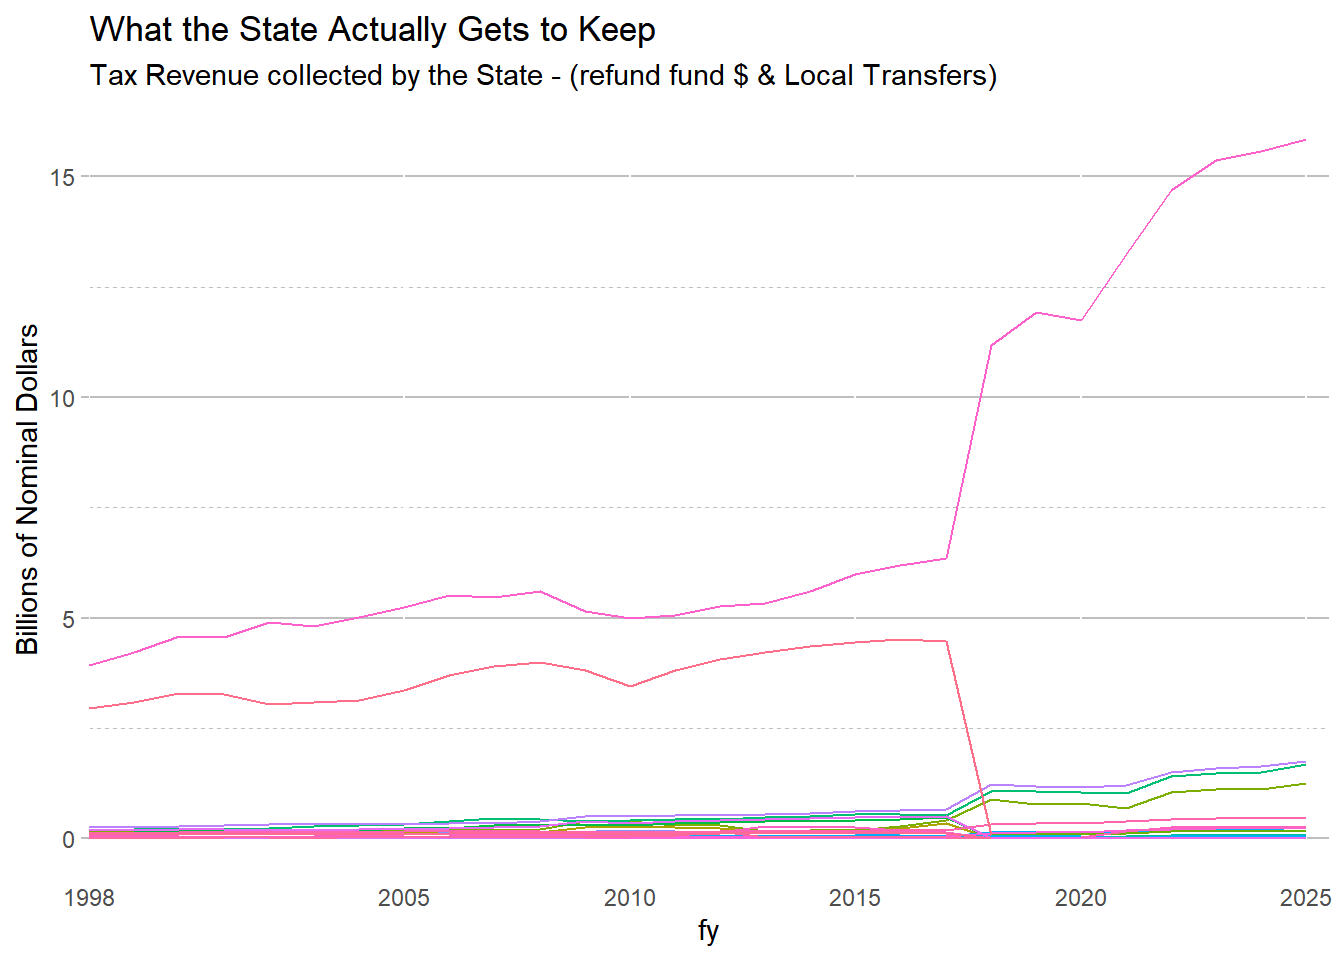
\includegraphics{./FedMoneyReceived_files/figure-pdf/unnamed-chunk-7-1.pdf}

}

\end{figure}

\begin{Shaded}
\begin{Highlighting}[]
\CommentTok{\# Color indicates state fund name. this way STate CURE funds are the same color from CARES and ARPA}
\FunctionTok{ggplot}\NormalTok{(sankey\_rev\_ioc, }
       \FunctionTok{aes}\NormalTok{(}\AttributeTok{y =}\NormalTok{ value, }\AttributeTok{axis3 =}\NormalTok{ Notes, }
         \CommentTok{\#  axis2 = stfundname, }
           \AttributeTok{axis1=}\NormalTok{Expenditures\_ordered, }\AttributeTok{label =} \StringTok{"stratum"}\NormalTok{)) }\SpecialCharTok{+}
  \FunctionTok{geom\_flow}\NormalTok{(}\FunctionTok{aes}\NormalTok{(}\AttributeTok{fill =}\NormalTok{ StateFunds), }\AttributeTok{color =} \StringTok{"black"}\NormalTok{,}\AttributeTok{reverse=}\ConstantTok{FALSE}\NormalTok{) }\SpecialCharTok{+}
  \FunctionTok{guides}\NormalTok{(}\AttributeTok{fill =} \ConstantTok{FALSE}\NormalTok{) }\SpecialCharTok{+}   
  \FunctionTok{geom\_stratum}\NormalTok{(}\AttributeTok{reverse=}\ConstantTok{FALSE}\NormalTok{)}\SpecialCharTok{+}
\FunctionTok{coord\_flip}\NormalTok{()}\SpecialCharTok{+}
   \FunctionTok{scale\_fill\_brewer}\NormalTok{(}\AttributeTok{palette =} \StringTok{"YlOrRd"}\NormalTok{, }\AttributeTok{direction =} \DecValTok{1}\NormalTok{)}\SpecialCharTok{+}
  \FunctionTok{theme\_void}\NormalTok{() }\SpecialCharTok{+}  
  \FunctionTok{theme}\NormalTok{(}\AttributeTok{legend.position=}\StringTok{"bottom"}\NormalTok{) }\SpecialCharTok{+}

  \FunctionTok{geom\_text}\NormalTok{(}\AttributeTok{stat =} \StringTok{"stratum"}\NormalTok{, }\FunctionTok{aes}\NormalTok{(}\AttributeTok{label =} \FunctionTok{after\_stat}\NormalTok{(stratum)), }\AttributeTok{size =} \DecValTok{2}\NormalTok{, }\AttributeTok{reverse=}\ConstantTok{FALSE}\NormalTok{)}\SpecialCharTok{+}
  \FunctionTok{labs}\NormalTok{(}\AttributeTok{title =} \StringTok{"Where the State CURE funds came from and other federal revenue received"}\NormalTok{,}
       \AttributeTok{caption =} \StringTok{"State CURE funds broken down by expenditure purpose in later graphs.}
\StringTok{       HPF = Healthcare Provider Fund"}\NormalTok{)}
\end{Highlighting}
\end{Shaded}

\begin{figure}[H]

{\centering 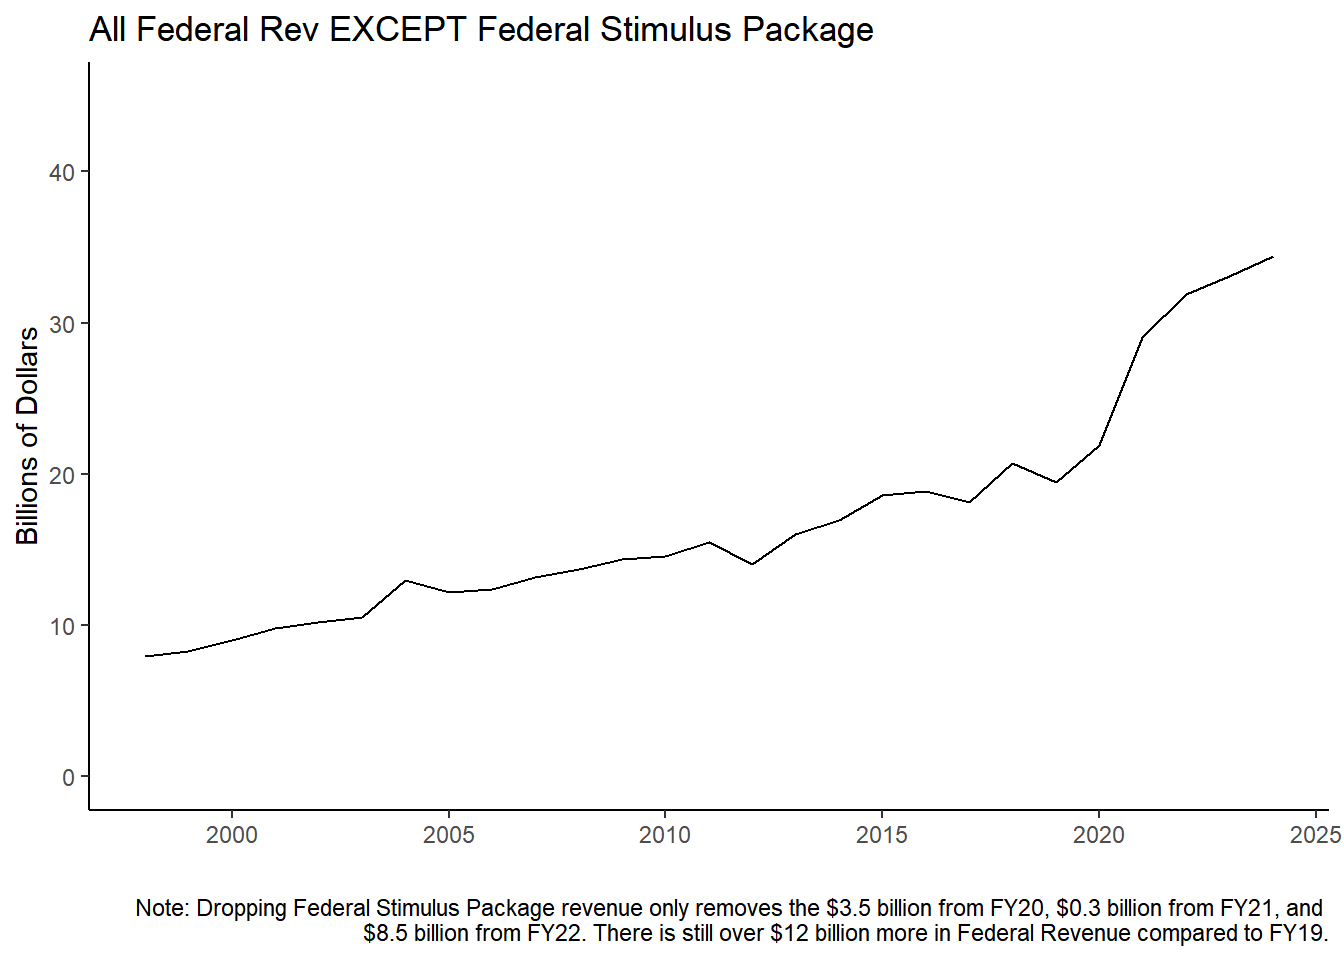
\includegraphics{./FedMoneyReceived_files/figure-pdf/unnamed-chunk-7-2.pdf}

}

\end{figure}

\begin{Shaded}
\begin{Highlighting}[]
\CommentTok{\# Color indicates state fund name. this way STate CURE funds are the same color from CARES and ARPA}
\FunctionTok{ggplot}\NormalTok{(sankey\_rev\_ioc, }
       \FunctionTok{aes}\NormalTok{(}\AttributeTok{y =}\NormalTok{ value, }\AttributeTok{axis3 =}\NormalTok{ Notes, }\AttributeTok{axis2 =}\NormalTok{ stfundname, }\AttributeTok{axis1=}\NormalTok{Expenditures\_ordered, }\AttributeTok{label =} \StringTok{"stratum"}\NormalTok{)) }\SpecialCharTok{+}
  \FunctionTok{geom\_flow}\NormalTok{(}\FunctionTok{aes}\NormalTok{(}\AttributeTok{fill =}\NormalTok{ stfundname), }\AttributeTok{color =} \StringTok{"black"}\NormalTok{,}\AttributeTok{reverse=}\ConstantTok{FALSE}\NormalTok{) }\SpecialCharTok{+}
  \FunctionTok{guides}\NormalTok{(}\AttributeTok{fill =} \ConstantTok{FALSE}\NormalTok{) }\SpecialCharTok{+}   
  \FunctionTok{geom\_stratum}\NormalTok{(}\AttributeTok{reverse=}\ConstantTok{FALSE}\NormalTok{)}\SpecialCharTok{+}
\FunctionTok{coord\_flip}\NormalTok{()}\SpecialCharTok{+}
   \FunctionTok{scale\_fill\_brewer}\NormalTok{(}\AttributeTok{palette =} \StringTok{"YlOrRd"}\NormalTok{, }\AttributeTok{direction =} \DecValTok{1}\NormalTok{)}\SpecialCharTok{+}
  \FunctionTok{theme\_void}\NormalTok{() }\SpecialCharTok{+}  
  \FunctionTok{theme}\NormalTok{(}\AttributeTok{legend.position=}\StringTok{"bottom"}\NormalTok{) }\SpecialCharTok{+}

 \CommentTok{\# geom\_text(stat = "stratum", aes(label = after\_stat(stratum)), size = 2, reverse=FALSE)+}
  \FunctionTok{labs}\NormalTok{(}\AttributeTok{title =} \StringTok{"Where the State CURE funds came from and other federal revenue received"}\NormalTok{,}
       \AttributeTok{caption =} \StringTok{"State CURE funds broken down by expenditure purpose in later graphs.}
\StringTok{       HPF = Healthcare Provider Fund"}\NormalTok{)}
\end{Highlighting}
\end{Shaded}

\begin{figure}[H]

{\centering 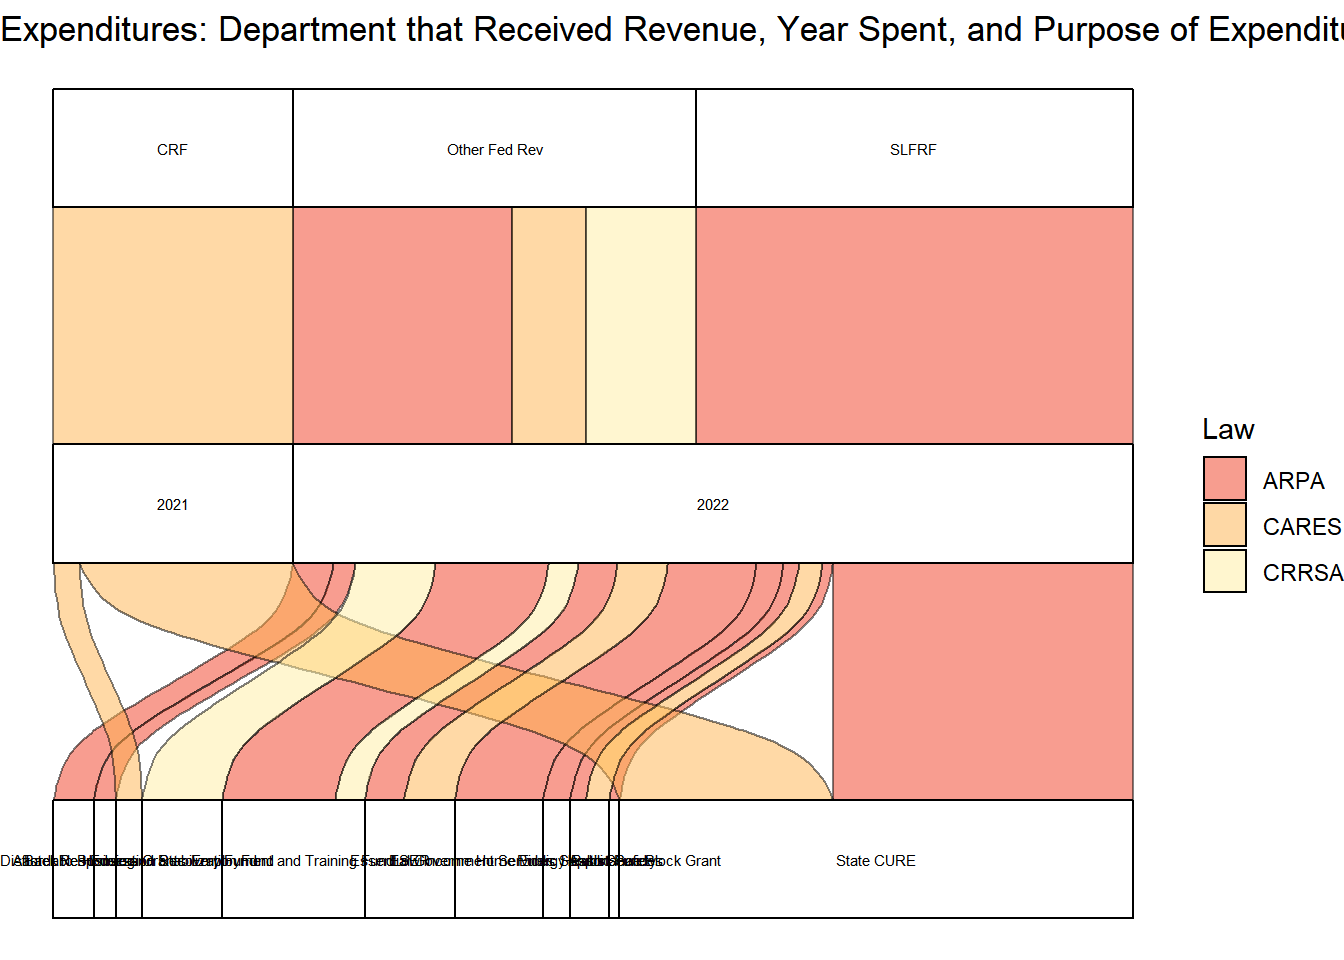
\includegraphics{./FedMoneyReceived_files/figure-pdf/unnamed-chunk-7-3.pdf}

}

\end{figure}

\begin{Shaded}
\begin{Highlighting}[]
\NormalTok{sankey\_rev\_ioc }\SpecialCharTok{\%\textgreater{}\%} \FunctionTok{group\_by}\NormalTok{(StateFunds, Expenditures) }\SpecialCharTok{\%\textgreater{}\%} 
  \FunctionTok{summarize}\NormalTok{(}\AttributeTok{sum=}\FunctionTok{sum}\NormalTok{(value))}
\end{Highlighting}
\end{Shaded}

\begin{verbatim}
# A tibble: 8 x 3
# Groups:   StateFunds [3]
  StateFunds          Expenditures        sum
  <fct>               <chr>             <dbl>
1 Total_received_fy20 Misc.        3518945000
2 Total_received_fy21 K-12          569467218
3 Total_received_fy21 Medicare     4926263219
4 Total_received_fy21 Other         561400000
5 Total_received_fy22 K-12         7305988054
6 Total_received_fy22 Medicare     4469242245
7 Total_received_fy22 Misc.        8127000000
8 Total_received_fy22 Other         664000000
\end{verbatim}

\begin{Shaded}
\begin{Highlighting}[]
\NormalTok{sankey\_rev\_ioc }\SpecialCharTok{\%\textgreater{}\%} \FunctionTok{group\_by}\NormalTok{(Expenditures) }\SpecialCharTok{\%\textgreater{}\%} 
  \FunctionTok{summarize}\NormalTok{(}\AttributeTok{sum=}\FunctionTok{sum}\NormalTok{(value))}
\end{Highlighting}
\end{Shaded}

\begin{verbatim}
# A tibble: 4 x 2
  Expenditures         sum
  <chr>              <dbl>
1 K-12          7875455272
2 Medicare      9395505464
3 Misc.        11645945000
4 Other         1225400000
\end{verbatim}

\begin{Shaded}
\begin{Highlighting}[]
\NormalTok{sankey\_rev\_ioc }\SpecialCharTok{\%\textgreater{}\%} \FunctionTok{group\_by}\NormalTok{( Notes, Federal, StateFunds, FF\_Cat) }\SpecialCharTok{\%\textgreater{}\%} 
  \FunctionTok{summarize}\NormalTok{(}\AttributeTok{sum=}\FunctionTok{sum}\NormalTok{(value))}
\end{Highlighting}
\end{Shaded}

\begin{verbatim}
# A tibble: 9 x 5
# Groups:   Notes, Federal, StateFunds [7]
  Notes Federal                   StateFunds          FF_Cat               sum
  <fct> <chr>                     <fct>               <chr>              <dbl>
1 CARES Federal Stimulus Packages Total_received_fy20 Federal Other 3518945000
2 CARES Other Federal Revenue     Total_received_fy21 Federal Other  626867218
3 CARES Other Federal Revenue     Total_received_fy21 Medicare      2636263219
4 PPP   Other Federal Revenue     Total_received_fy21 Federal Other  504000000
5 PPP   Other Federal Revenue     Total_received_fy21 Medicare      2290000000
6 FFCRA Other Federal Revenue     Total_received_fy22 Medicare      4469242245
7 CRRSA Other Federal Revenue     Total_received_fy22 Federal Other 2915000000
8 ARPA  Federal Stimulus Packages Total_received_fy22 Federal Other 8127000000
9 ARPA  Other Federal Revenue     Total_received_fy22 Federal Other 5054988054
\end{verbatim}

\begin{Shaded}
\begin{Highlighting}[]
\CommentTok{\# Color indicates legislation}
\FunctionTok{ggplot}\NormalTok{(sankey\_rev\_ioc, }
       \FunctionTok{aes}\NormalTok{(}\AttributeTok{y =}\NormalTok{ value, }\AttributeTok{axis4 =}\NormalTok{ Federal, }\AttributeTok{axis3 =}\NormalTok{ Notes, }\AttributeTok{axis2 =}\NormalTok{ stfundname, }\AttributeTok{axis1=}\NormalTok{Expenditures, }\AttributeTok{label =} \StringTok{"stratum"}\NormalTok{)) }\SpecialCharTok{+}
  \FunctionTok{geom\_flow}\NormalTok{(}\FunctionTok{aes}\NormalTok{(}\AttributeTok{fill =}\NormalTok{ Notes), }\AttributeTok{color =} \StringTok{"black"}\NormalTok{,}\AttributeTok{reverse=}\ConstantTok{FALSE}\NormalTok{) }\SpecialCharTok{+}
  \FunctionTok{guides}\NormalTok{(}\AttributeTok{fill =} \ConstantTok{FALSE}\NormalTok{) }\SpecialCharTok{+}   
  \FunctionTok{geom\_stratum}\NormalTok{(}\AttributeTok{reverse=}\ConstantTok{FALSE}\NormalTok{)}\SpecialCharTok{+}
\FunctionTok{coord\_flip}\NormalTok{()}\SpecialCharTok{+}
   \FunctionTok{scale\_fill\_brewer}\NormalTok{(}\AttributeTok{palette =} \StringTok{"YlOrRd"}\NormalTok{, }\AttributeTok{direction =} \SpecialCharTok{{-}}\DecValTok{1}\NormalTok{)}\SpecialCharTok{+}
  \FunctionTok{theme\_void}\NormalTok{() }\SpecialCharTok{+}  
  \FunctionTok{theme}\NormalTok{(}\AttributeTok{legend.position=}\StringTok{"bottom"}\NormalTok{) }\SpecialCharTok{+}

  \FunctionTok{geom\_text}\NormalTok{(}\AttributeTok{stat =} \StringTok{"stratum"}\NormalTok{, }\FunctionTok{aes}\NormalTok{(}\AttributeTok{label =} \FunctionTok{after\_stat}\NormalTok{(stratum)), }\AttributeTok{size =} \DecValTok{2}\NormalTok{, }\AttributeTok{reverse=}\ConstantTok{FALSE}\NormalTok{)}\SpecialCharTok{+}
  \FunctionTok{labs}\NormalTok{(}\AttributeTok{title =} \StringTok{"$32 Billion in Federal Funds Received, Legislation, State Fund }
\StringTok{       that Received Money, and FF Expenditure Category"}\NormalTok{,}
       \AttributeTok{caption =} \StringTok{"State CURE funds broken down by expenditure purpose in later graphs.}
\StringTok{       HPF = Healthcare Provider Fund"}\NormalTok{)}
\end{Highlighting}
\end{Shaded}

\begin{figure}[H]

{\centering 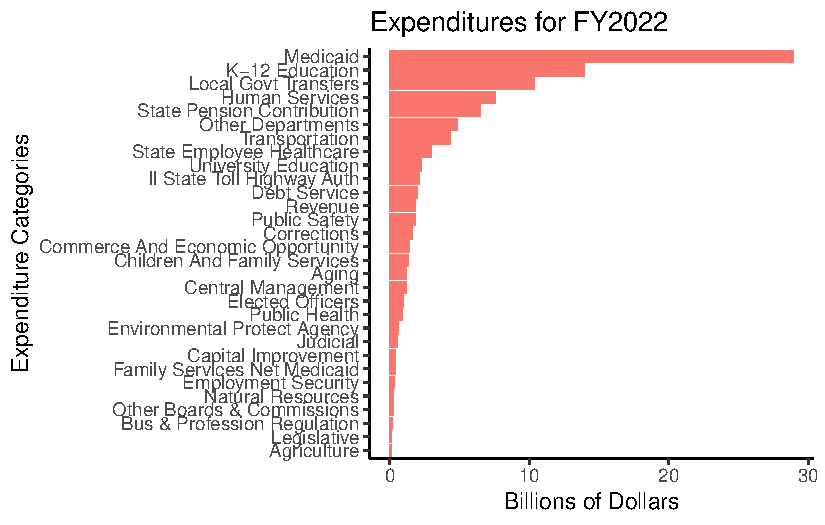
\includegraphics{./FedMoneyReceived_files/figure-pdf/unnamed-chunk-8-1.pdf}

}

\end{figure}

\begin{Shaded}
\begin{Highlighting}[]
\CommentTok{\# Same as graph above but gets rid of top axis for federal funds}
\CommentTok{\# Color indicates State CURE funds or State Departments grants}
\CommentTok{\# ggplot(sankey\_rev\_ioc, }
\CommentTok{\#        aes(y = value, axis3 = Notes, axis2 = stfundname, axis1=Expenditures, label = "stratum")) +}
\CommentTok{\#   geom\_flow(aes(fill = Federal), color = "black", reverse=FALSE) +}
\CommentTok{\#   guides(fill = FALSE) +   }
\CommentTok{\#   geom\_stratum(reverse=FALSE)+}
\CommentTok{\#   coord\_flip()+}
\CommentTok{\#   scale\_fill\_brewer(palette = "YlOrRd", direction = {-}1)+}
\CommentTok{\#   theme(legend.position="bottom") +}
\CommentTok{\#   }
\CommentTok{\#   theme\_void() +  }
\CommentTok{\#   }
\CommentTok{\#   geom\_text(stat = "stratum", aes(label = after\_stat(stratum)), size = 2, reverse=FALSE) +}
\CommentTok{\#   }
\CommentTok{\#   labs(title = "$32 Billion in Federal Funds Received, Legislation, State Fund }
\CommentTok{\#        that Received Money, and FF Expenditure Category",}
\CommentTok{\#        caption = "State CURE funds broken down by expenditure purpose in later graphs.}
\CommentTok{\#        HPF = Healthcare Provider Fund.}
\CommentTok{\#        Color indicates State CURE funds and Grants to State Department.")}
\end{Highlighting}
\end{Shaded}

Highlights legislation, fund money went into, and its intended purpose
using Fiscal Futures expenditure categories. The State CURE expenditures
are listed as miscellaneous here but are described in more detail
farther below.

\begin{Shaded}
\begin{Highlighting}[]
\CommentTok{\# color indicates fund}
\FunctionTok{ggplot}\NormalTok{(sankey\_rev\_ioc, }
       \FunctionTok{aes}\NormalTok{(}\AttributeTok{y =}\NormalTok{ value, }\AttributeTok{axis3 =}\NormalTok{ Notes, }\AttributeTok{axis2 =}\NormalTok{ stfundname, }\AttributeTok{axis1=}\NormalTok{Expenditures, }\AttributeTok{label =} \StringTok{"stratum"}\NormalTok{)) }\SpecialCharTok{+}
  \FunctionTok{geom\_flow}\NormalTok{(}\FunctionTok{aes}\NormalTok{(}\AttributeTok{fill =}\NormalTok{ stfundname), }\AttributeTok{color =} \StringTok{"black"}\NormalTok{, }\AttributeTok{reverse=}\ConstantTok{FALSE}\NormalTok{) }\SpecialCharTok{+}
  \FunctionTok{geom\_stratum}\NormalTok{(}\AttributeTok{reverse=}\ConstantTok{FALSE}\NormalTok{)}\SpecialCharTok{+}
\FunctionTok{coord\_flip}\NormalTok{()}\SpecialCharTok{+}
   \FunctionTok{scale\_fill\_brewer}\NormalTok{(}\AttributeTok{palette =} \StringTok{"YlOrRd"}\NormalTok{, }\AttributeTok{direction =} \SpecialCharTok{{-}}\DecValTok{1}\NormalTok{)}\SpecialCharTok{+}
  \FunctionTok{theme\_void}\NormalTok{() }\SpecialCharTok{+}
  \FunctionTok{theme}\NormalTok{(}\AttributeTok{legend.position=}\StringTok{"bottom"}\NormalTok{) }\SpecialCharTok{+}

      \FunctionTok{geom\_text}\NormalTok{(}\AttributeTok{stat =} \StringTok{"stratum"}\NormalTok{, }\FunctionTok{aes}\NormalTok{(}\AttributeTok{label =} \FunctionTok{after\_stat}\NormalTok{(stratum)), }\AttributeTok{size =} \DecValTok{2}\NormalTok{,}\AttributeTok{reverse=}\ConstantTok{FALSE}\NormalTok{) }\SpecialCharTok{+}
   \FunctionTok{labs}\NormalTok{(}\AttributeTok{title =} \StringTok{"Legislation that provided funds, state fund receiving revenue, }
\StringTok{   and how funds were used"}\NormalTok{, }\AttributeTok{caption =} \StringTok{"State CURE expenditures are not broken down in this image for readibility. }
\StringTok{         Please see graphs focused on State CURE expenditures below."}\NormalTok{)}
\end{Highlighting}
\end{Shaded}

\begin{figure}[H]

{\centering 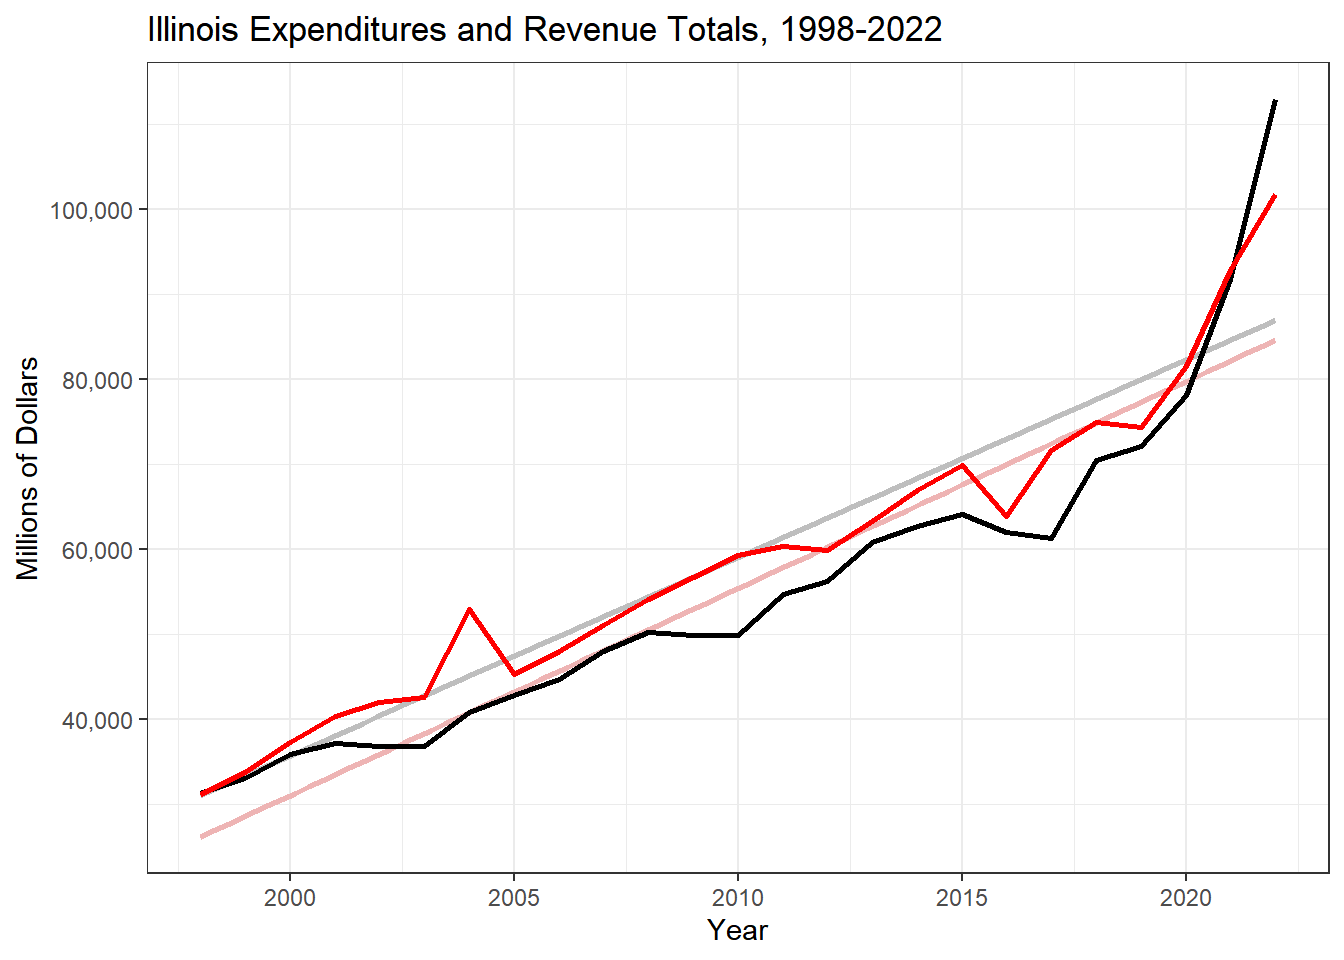
\includegraphics{./FedMoneyReceived_files/figure-pdf/unnamed-chunk-9-1.pdf}

}

\end{figure}

\begin{tcolorbox}[enhanced jigsaw, coltitle=black, titlerule=0mm, leftrule=.75mm, colbacktitle=quarto-callout-important-color!10!white, arc=.35mm, rightrule=.15mm, opacityback=0, colframe=quarto-callout-important-color-frame, toptitle=1mm, opacitybacktitle=0.6, bottomtitle=1mm, title={Important}, colback=white, breakable, toprule=.15mm, left=2mm, bottomrule=.15mm]

Remember: Medicare includes Healthcare Provider Assistance,
reimbursements for the Continuous Coverage Mandate, and reimbursements
for the Matching Funds Increase. This is different than GOMB
categorization.

\end{tcolorbox}

These revenue graphs label State CURE as being for miscellaneous
purposes due to the difficulty of representing that information broken
down cleanly in the graphs. To see how ARPA funds (and State CURE funds
in general) were spent, jump to
Section~\ref{sec-state-expenditure-graphs}.

\begin{Shaded}
\begin{Highlighting}[]
\FunctionTok{ggplot}\NormalTok{(sankey\_rev\_ioc, }
       \FunctionTok{aes}\NormalTok{(}\AttributeTok{y =}\NormalTok{ value, }
           \AttributeTok{axis3 =}\NormalTok{ Notes, }\AttributeTok{axis2 =}\NormalTok{ StateFunds, }\AttributeTok{axis1=}\NormalTok{Expenditures, }\AttributeTok{label =} \StringTok{"stratum"}\NormalTok{)) }\SpecialCharTok{+}
  \FunctionTok{geom\_flow}\NormalTok{(}\FunctionTok{aes}\NormalTok{(}\AttributeTok{fill =}\NormalTok{ stfundname), }\AttributeTok{color =} \StringTok{"black"}\NormalTok{, }\AttributeTok{reverse=}\ConstantTok{FALSE}\NormalTok{) }\SpecialCharTok{+}
  \FunctionTok{geom\_stratum}\NormalTok{(}\AttributeTok{reverse=}\ConstantTok{FALSE}\NormalTok{)}\SpecialCharTok{+}
\FunctionTok{coord\_flip}\NormalTok{()}\SpecialCharTok{+}
   \FunctionTok{scale\_fill\_brewer}\NormalTok{(}\AttributeTok{palette =} \StringTok{"YlOrRd"}\NormalTok{, }\AttributeTok{direction =} \SpecialCharTok{{-}}\DecValTok{1}\NormalTok{)}\SpecialCharTok{+}
  \FunctionTok{theme\_void}\NormalTok{() }\SpecialCharTok{+}
  \FunctionTok{theme}\NormalTok{(}\AttributeTok{legend.position=}\StringTok{"bottom"}\NormalTok{) }\SpecialCharTok{+}

      \FunctionTok{geom\_text}\NormalTok{(}\AttributeTok{stat =} \StringTok{"stratum"}\NormalTok{, }\FunctionTok{aes}\NormalTok{(}\AttributeTok{label =} \FunctionTok{after\_stat}\NormalTok{(stratum)), }\AttributeTok{size =} \DecValTok{2}\NormalTok{, }\AttributeTok{reverse =} \ConstantTok{FALSE}\NormalTok{)}
\end{Highlighting}
\end{Shaded}

\begin{figure}[H]

{\centering 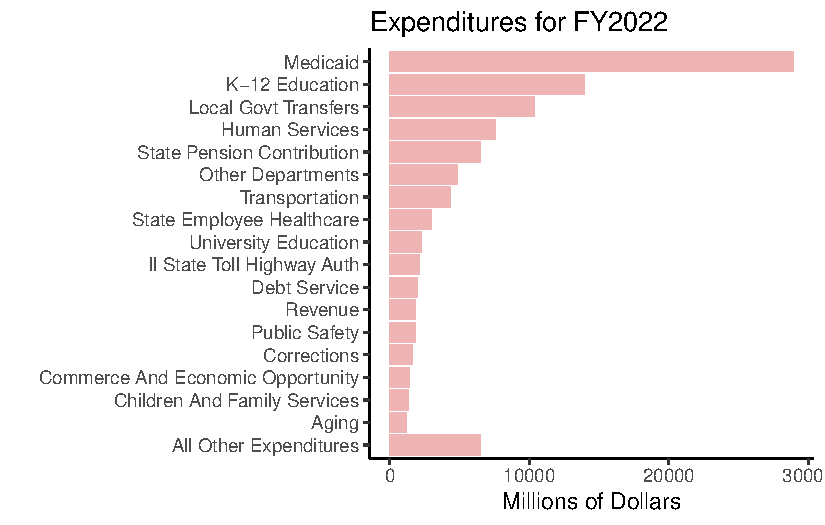
\includegraphics{./FedMoneyReceived_files/figure-pdf/unnamed-chunk-10-1.pdf}

}

\end{figure}

\begin{Shaded}
\begin{Highlighting}[]
\FunctionTok{ggplot}\NormalTok{(sankey\_rev\_ioc, }
       \FunctionTok{aes}\NormalTok{(}\AttributeTok{y =}\NormalTok{ value, }
           \AttributeTok{axis4 =}\NormalTok{ Notes, }\AttributeTok{axis3 =}\NormalTok{ StateFunds, }\AttributeTok{axis2=}\NormalTok{ Federal, }\AttributeTok{axis1=}\NormalTok{Expenditures, }\AttributeTok{label =} \StringTok{"stratum"}\NormalTok{)) }\SpecialCharTok{+}
  \FunctionTok{geom\_flow}\NormalTok{(}\FunctionTok{aes}\NormalTok{(}\AttributeTok{fill =}\NormalTok{ Notes), }\AttributeTok{color =} \StringTok{"black"}\NormalTok{, }\AttributeTok{reverse=}\ConstantTok{FALSE}\NormalTok{) }\SpecialCharTok{+}
  \FunctionTok{geom\_stratum}\NormalTok{(}\AttributeTok{reverse=}\ConstantTok{FALSE}\NormalTok{)}\SpecialCharTok{+}
\FunctionTok{coord\_flip}\NormalTok{()}\SpecialCharTok{+}
   \FunctionTok{scale\_fill\_brewer}\NormalTok{(}\AttributeTok{palette =} \StringTok{"YlOrRd"}\NormalTok{, }\AttributeTok{direction =} \SpecialCharTok{{-}}\DecValTok{1}\NormalTok{)}\SpecialCharTok{+}
  \FunctionTok{theme\_void}\NormalTok{() }\SpecialCharTok{+}
  \FunctionTok{theme}\NormalTok{(}\AttributeTok{legend.position=}\StringTok{"bottom"}\NormalTok{) }\SpecialCharTok{+}

      \FunctionTok{geom\_text}\NormalTok{(}\AttributeTok{stat =} \StringTok{"stratum"}\NormalTok{, }\FunctionTok{aes}\NormalTok{(}\AttributeTok{label =} \FunctionTok{after\_stat}\NormalTok{(stratum)), }\AttributeTok{size =} \DecValTok{2}\NormalTok{, }\AttributeTok{reverse =} \ConstantTok{FALSE}\NormalTok{)}
\end{Highlighting}
\end{Shaded}

\begin{figure}[H]

{\centering 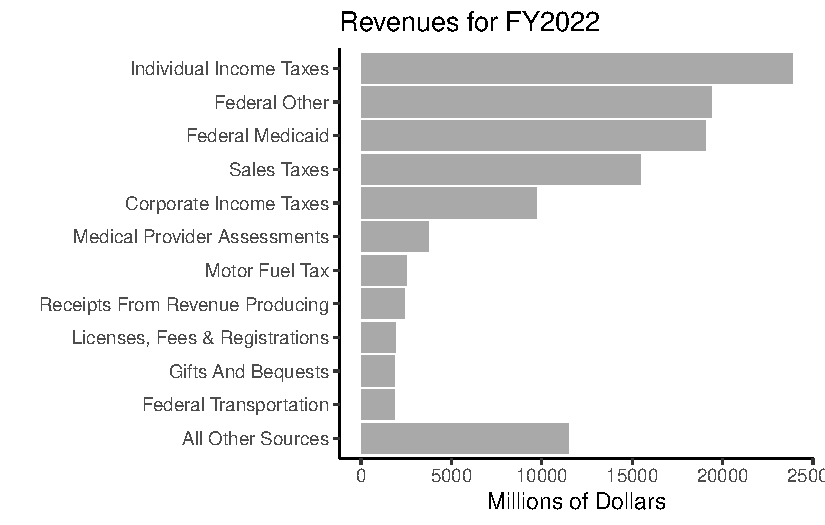
\includegraphics{./FedMoneyReceived_files/figure-pdf/unnamed-chunk-10-2.pdf}

}

\end{figure}

\begin{quote}
\begin{tcolorbox}[enhanced jigsaw, coltitle=black, titlerule=0mm, leftrule=.75mm, colbacktitle=quarto-callout-note-color!10!white, arc=.35mm, rightrule=.15mm, opacityback=0, colframe=quarto-callout-note-color-frame, toptitle=1mm, opacitybacktitle=0.6, bottomtitle=1mm, title=\textcolor{quarto-callout-note-color}{\faInfo}\hspace{0.5em}{Note}, colback=white, breakable, toprule=.15mm, left=2mm, bottomrule=.15mm]

Note: CARES funds were originally received and spent in Disaster
Response \& Recovery Fund. In FY22, unspent aid was transferred to the
State CURE and then transferred again to state agencies for
COVID-related expenditures. Remaining CARES funds were transferred to
State CURE fund for FY22. \$337 million was also transferred from the
Illinois Department of Revenue into the Illinois Housing Development
Authority (IHDA).
(\href{https://budget.illinois.gov/content/dam/soi/en/web/budget/documents/lboc/lboc-report-june-2021-final.pdf}{LBOC
June 2021 Report}).

\end{tcolorbox}
\end{quote}

\hypertarget{sec-state-expenditure-graphs}{%
\section{State Expenditure Graphs}\label{sec-state-expenditure-graphs}}

Federal expenditures from CURE and other major funds . Uses the
\texttt{fedCUREexpenditures.xlsx} file.

This data comes from Illinois Comptroller expenditure data, Legislative
Budget Oversight Commission (LBOC) Reports, and the
\href{https://budget.illinois.gov/content/dam/soi/en/web/budget/documents/arpa/IL\%20Recovery\%20Plan\%20Performance\%20Report\%202022.pdf}{ARPA
Annual Recovery Plan} detailing the State's use of State and Local
Fiscal Recovery Funds (SLFRF) which is prepared by the Governor's Office
of Management and Budget (GOMB).

Dates on top are Fiscal Year received. Dates in the middle of the graph
are Fiscal Year expenditures. Remember, federal funds for COVID recovery
have been received and spent in different years.

Revenue from Local Cure is the Local Government Transfers. A small
amount of the State CURE was also transferred to local governments
(\$240 million in FY2021). There was also \$700 million ARPA State CURE
funds transferred to local governments during FY21 and FY22.

\hypertarget{fiscal-years-2020-2022}{%
\subsection{Fiscal Years 2020-2022}\label{fiscal-years-2020-2022}}

During fiscal years 2020 through 2022 \$11.03 billion (\$8.4 CURE +
\$3.082 ESSER) in State CURE and ESSER funds have been spent by the
state. An additional \$6.9 billion of grants from CARES, CRRSA, and ARPA
has been spent by state departments.

So far, over \$8.4 billion of the State CURE funds (includes both CARES
Act and ARP Act State Fiscal Recovery Fund) have been spent in
FY2020-2022.

\textbf{CARES State CURE money:}

\begin{itemize}
\tightlist
\item
  \$370 million was spent in the initial pandemic response in the very
  end of FY2020 and \$2.858 billion CARES dollars were spent in FY21.
\item
  In FY2022, almost all remaining CARES funds were used up
  (\textasciitilde250 million).
\item
  Around \$3.5 billion total spent during FY20-FY22.
\end{itemize}

\textbf{ARPA State CURE money:}

\begin{itemize}
\item
  In FY22, \$4.9 billion (of \$8.127 billion received) ARPA-State CURE
  dollars were spent:

  \begin{itemize}
  \tightlist
  \item
    \$2.7 billion for repaying unemployment insurance trust fund, \$1
    billion transferred to the general revenue fund to make up for any
    lost revenue caused by the pandemic, and \$1.23 billion on other
    programs and services (e.g.~hospital stability payments, operational
    expenses, back to business grants and economic development).
  \end{itemize}
\end{itemize}

Values presented in LBOC documents for the end of FY22 are slightly
different than the values calculated using IOC expenditure data. IOC
expenditure data includes all lag period expenditures through October so
values are slightly higher than end of June calculations.

\begin{Shaded}
\begin{Highlighting}[]
\NormalTok{cure\_exp }\OtherTok{\textless{}{-}} \FunctionTok{read\_xlsx}\NormalTok{(}\StringTok{"fedCUREexpenditures.xlsx"}\NormalTok{)}

\NormalTok{cure\_exp2022 }\OtherTok{\textless{}{-}}\NormalTok{ cure\_exp }\SpecialCharTok{\%\textgreater{}\%}
  \FunctionTok{filter}\NormalTok{(FY\_Spent }\SpecialCharTok{\textless{}}\DecValTok{2023}\NormalTok{) }\SpecialCharTok{\%\textgreater{}\%} \CommentTok{\# excludes FY23 and beyond}
  
  \FunctionTok{mutate}\NormalTok{(}
         \AttributeTok{FY\_Spent =} \FunctionTok{factor}\NormalTok{(FY\_Spent, }\AttributeTok{levels =} \FunctionTok{c}\NormalTok{(}\StringTok{"2020"}\NormalTok{, }\StringTok{"2021"}\NormalTok{, }\StringTok{"2022"}\NormalTok{)),}
         \AttributeTok{FY\_Received =} \FunctionTok{factor}\NormalTok{(FY\_Received, }\AttributeTok{levels =} \FunctionTok{c}\NormalTok{(}\StringTok{"2020"}\NormalTok{, }\StringTok{"2021"}\NormalTok{, }\StringTok{"2022"}\NormalTok{))}\CommentTok{\#,}
      \CommentTok{\#   FF\_Cat = factor(FF\_Cat, levels = c("Econ Dev", "Human Services", "K{-}12", "Local Transfers", "Public Health", "Medicaid", "Public Safety",  "UI Fund", "Lost Revenue")),}
     \CommentTok{\#    FF\_Cat2 = factor(FF\_Cat, levels = c("Econ Dev", "Human Services", "K{-}12", "Local Transfers", "Public Health \& Safety", "Medicare",  "UI Fund", "Lost Revenue", "FY23+"))}
\NormalTok{     )}



\NormalTok{cure\_exp2022 }\SpecialCharTok{\%\textgreater{}\%} \CommentTok{\#expenditures per year}
  \FunctionTok{filter}\NormalTok{(State\_local }\SpecialCharTok{==} \StringTok{"State CURE"}\NormalTok{) }\SpecialCharTok{\%\textgreater{}\%}
  \FunctionTok{group\_by}\NormalTok{(}\StringTok{\textasciigrave{}}\AttributeTok{FY\_Spent}\StringTok{\textasciigrave{}}\NormalTok{)}\SpecialCharTok{\%\textgreater{}\%} 
  \FunctionTok{summarize}\NormalTok{(}\AttributeTok{Expenditures=}\FunctionTok{sum}\NormalTok{(}\StringTok{\textasciigrave{}}\AttributeTok{FY Expenditures}\StringTok{\textasciigrave{}}\NormalTok{))}
\end{Highlighting}
\end{Shaded}

\begin{verbatim}
# A tibble: 3 x 2
  FY_Spent Expenditures
  <fct>           <dbl>
1 2020              370
2 2021             2858
3 2022             5173
\end{verbatim}

\begin{Shaded}
\begin{Highlighting}[]
\CommentTok{\# State CURE expenditures only}
\NormalTok{cure\_exp2022}\SpecialCharTok{\%\textgreater{}\%}  
    \FunctionTok{filter}\NormalTok{(State\_local }\SpecialCharTok{==} \StringTok{"State CURE"}\NormalTok{) }\SpecialCharTok{\%\textgreater{}\%}
  \FunctionTok{summarize}\NormalTok{(}\AttributeTok{Expenditures=}\FunctionTok{sum}\NormalTok{(}\StringTok{\textasciigrave{}}\AttributeTok{FY Expenditures}\StringTok{\textasciigrave{}}\NormalTok{)) }
\end{Highlighting}
\end{Shaded}

\begin{verbatim}
# A tibble: 1 x 1
  Expenditures
         <dbl>
1         8401
\end{verbatim}

\begin{Shaded}
\begin{Highlighting}[]
\NormalTok{cure\_exp2022 }\SpecialCharTok{\%\textgreater{}\%} 
  \FunctionTok{filter}\NormalTok{(State\_local }\SpecialCharTok{==} \StringTok{"State CURE"}\NormalTok{) }\SpecialCharTok{\%\textgreater{}\%}
  \FunctionTok{group\_by}\NormalTok{(Law, FF\_Cat2)}\SpecialCharTok{\%\textgreater{}\%} 
  \FunctionTok{summarize}\NormalTok{(}\AttributeTok{Expenditures=}\FunctionTok{sum}\NormalTok{(}\StringTok{\textasciigrave{}}\AttributeTok{FY Expenditures}\StringTok{\textasciigrave{}}\NormalTok{)) }\SpecialCharTok{\%\textgreater{}\%}
  \FunctionTok{pivot\_wider}\NormalTok{(}\AttributeTok{names\_from =}\NormalTok{ Law, }\AttributeTok{values\_from =}\NormalTok{ Expenditures)}
\end{Highlighting}
\end{Shaded}

\begin{verbatim}
# A tibble: 8 x 3
  FF_Cat2                 ARPA CARES
  <chr>                  <dbl> <dbl>
1 Econ Dev                 937   660
2 Lost Revenue            1000    NA
3 Public Health & Safety   290   430
4 UI Fund                 2700    NA
5 Human Services            NA   260
6 Local Transfers           NA   240
7 Medicare                  NA   705
8 Reimbursements            NA  1179
\end{verbatim}

Code chunk below is for State CURE funds spent through FY 2022.

\begin{Shaded}
\begin{Highlighting}[]
\CommentTok{\# State CURE only, }
\CommentTok{\# without 2023 allocations}

\NormalTok{cure\_exp2022 }\SpecialCharTok{\%\textgreater{}\%} 
  \FunctionTok{filter}\NormalTok{(State\_local }\SpecialCharTok{==} \StringTok{"State CURE"}\NormalTok{) }\SpecialCharTok{\%\textgreater{}\%} \CommentTok{\# for only state CURE funds}
  \FunctionTok{ggplot}\NormalTok{(}\FunctionTok{aes}\NormalTok{(}\AttributeTok{y =} \StringTok{\textasciigrave{}}\AttributeTok{FY Expenditures}\StringTok{\textasciigrave{}}\NormalTok{, }\AttributeTok{axis4 =}\NormalTok{ FY\_Received, }\AttributeTok{axis3 =} \StringTok{\textasciigrave{}}\AttributeTok{Agency}\StringTok{\textasciigrave{}}\NormalTok{,  }
             \AttributeTok{axis2 =}\NormalTok{ FY\_Spent, }\AttributeTok{axis1=}\NormalTok{FF\_Cat2, }\AttributeTok{label =} \StringTok{"stratum"}\NormalTok{)) }\SpecialCharTok{+}
  \FunctionTok{geom\_flow}\NormalTok{(}\FunctionTok{aes}\NormalTok{(}\AttributeTok{fill =}\NormalTok{ FF\_Cat2), }\AttributeTok{color =} \StringTok{"black"}\NormalTok{, }\AttributeTok{reverse=}\ConstantTok{FALSE}\NormalTok{) }\SpecialCharTok{+}
  \FunctionTok{geom\_stratum}\NormalTok{(}\AttributeTok{reverse=}\ConstantTok{FALSE}\NormalTok{)}\SpecialCharTok{+}
  \FunctionTok{coord\_flip}\NormalTok{()}\SpecialCharTok{+}
  \FunctionTok{scale\_fill\_brewer}\NormalTok{(}\AttributeTok{palette =} \StringTok{"YlOrRd"}\NormalTok{, }\AttributeTok{direction =} \SpecialCharTok{{-}}\DecValTok{1}\NormalTok{)}\SpecialCharTok{+}
  \FunctionTok{theme\_void}\NormalTok{() }\SpecialCharTok{+} 
  \FunctionTok{theme}\NormalTok{(}\AttributeTok{legend.position=}\StringTok{"bottom"}\NormalTok{)}\SpecialCharTok{+}
  
  \FunctionTok{geom\_text}\NormalTok{(}\AttributeTok{stat =} \StringTok{"stratum"}\NormalTok{, }\FunctionTok{aes}\NormalTok{(}\AttributeTok{label =} \FunctionTok{after\_stat}\NormalTok{(stratum)), }\AttributeTok{size =} \DecValTok{2}\NormalTok{, }\AttributeTok{reverse=}\ConstantTok{FALSE}\NormalTok{) }\SpecialCharTok{+}
  \FunctionTok{labs}\NormalTok{(}\AttributeTok{title =} \StringTok{"Expenditures using State CURE funds: $8.4 spent FY20{-}FY22"}\NormalTok{, }
  \AttributeTok{subtitle =} \StringTok{"Year Received by State Department, Year Spent, and how it was spent so far"}\NormalTok{, }
  \AttributeTok{caption =} \StringTok{"Expenditures occured during FY20, FY21 and FY22. }
\StringTok{       Additional funds have been allocated for FY23 and can be spent until FY26.}
\StringTok{  Public Health \& Public Safety combined due to overlap with IEMA\textquotesingle{}s involvemnt in pandemic response."}\NormalTok{)}
\end{Highlighting}
\end{Shaded}

\begin{figure}[H]

{\centering 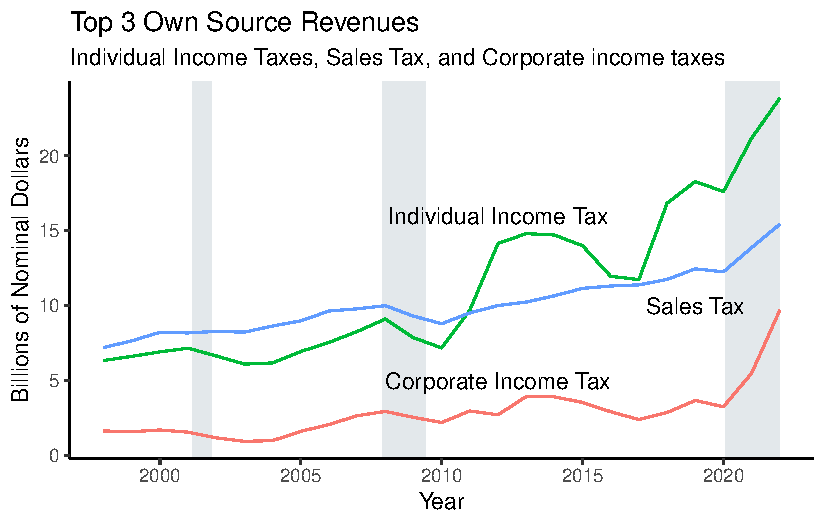
\includegraphics{./FedMoneyReceived_files/figure-pdf/unnamed-chunk-12-1.pdf}

}

\end{figure}

\begin{Shaded}
\begin{Highlighting}[]
\DocumentationTok{\#\# State CURE only}
\CommentTok{\# through FY22}
\NormalTok{cure\_exp2022 }\SpecialCharTok{\%\textgreater{}\%} 
  \FunctionTok{filter}\NormalTok{(State\_local }\SpecialCharTok{==} \StringTok{"State CURE"}\NormalTok{) }\SpecialCharTok{\%\textgreater{}\%} 
  \FunctionTok{ggplot}\NormalTok{(}\FunctionTok{aes}\NormalTok{(}\AttributeTok{y =} \StringTok{\textasciigrave{}}\AttributeTok{FY Expenditures}\StringTok{\textasciigrave{}}\NormalTok{, }\AttributeTok{axis3 =} \StringTok{\textasciigrave{}}\AttributeTok{State\_local2}\StringTok{\textasciigrave{}}\NormalTok{, }\AttributeTok{axis2 =}\NormalTok{ Agency\_grouped, }\AttributeTok{axis1=}\NormalTok{FF\_Cat2, }\AttributeTok{label =} \StringTok{"stratum"}\NormalTok{))}\SpecialCharTok{+}
  \FunctionTok{geom\_flow}\NormalTok{(}\FunctionTok{aes}\NormalTok{(}\AttributeTok{fill =}\NormalTok{ Law), }\AttributeTok{color =} \StringTok{"black"}\NormalTok{, }\AttributeTok{reverse=}\ConstantTok{FALSE}\NormalTok{) }\SpecialCharTok{+}
  \FunctionTok{geom\_stratum}\NormalTok{(}\AttributeTok{reverse=}\ConstantTok{FALSE}\NormalTok{)}\SpecialCharTok{+}
 \FunctionTok{coord\_flip}\NormalTok{()}\SpecialCharTok{+}
   \FunctionTok{scale\_fill\_brewer}\NormalTok{(}\AttributeTok{palette =} \StringTok{"YlOrRd"}\NormalTok{, }\AttributeTok{direction =} \SpecialCharTok{{-}}\DecValTok{1}\NormalTok{)}\SpecialCharTok{+}
  \FunctionTok{theme\_void}\NormalTok{() }\SpecialCharTok{+} 
  \FunctionTok{theme}\NormalTok{(}\AttributeTok{legend.position=}\StringTok{"bottom"}\NormalTok{)}\SpecialCharTok{+}
  \FunctionTok{geom\_text}\NormalTok{(}\AttributeTok{stat =} \StringTok{"stratum"}\NormalTok{, }\FunctionTok{aes}\NormalTok{(}\AttributeTok{label =} \FunctionTok{after\_stat}\NormalTok{(stratum)), }\AttributeTok{size =} \DecValTok{2}\NormalTok{, }\AttributeTok{reverse=}\ConstantTok{FALSE}\NormalTok{) }\SpecialCharTok{+}
  \FunctionTok{theme}\NormalTok{(}\AttributeTok{legend.position=}\StringTok{"bottom"}\NormalTok{)}\SpecialCharTok{+}

  \FunctionTok{labs}\NormalTok{(}\AttributeTok{title =} \StringTok{"State CURE Expenditures: Department that Received Revenue}
\StringTok{       \& Purpose of Expenditure"}\NormalTok{,}
       \AttributeTok{subtitle =} \StringTok{"$8.4 billion spent by end of FY22"}\NormalTok{)}
\end{Highlighting}
\end{Shaded}

\begin{figure}[H]

{\centering 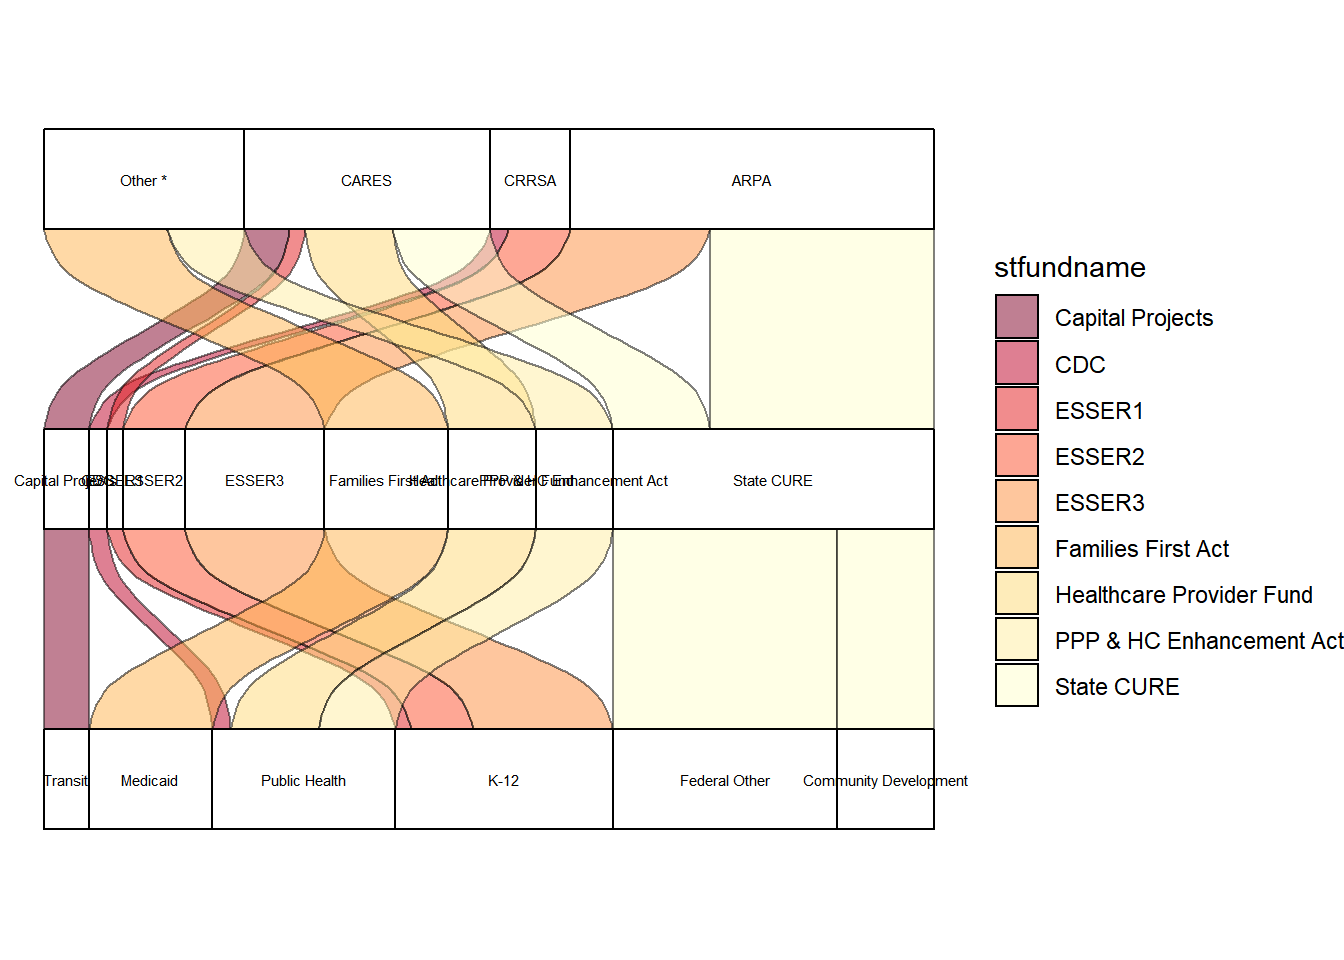
\includegraphics{./FedMoneyReceived_files/figure-pdf/unnamed-chunk-12-2.pdf}

}

\end{figure}

\begin{Shaded}
\begin{Highlighting}[]
\NormalTok{cure\_exp2022 }\SpecialCharTok{\%\textgreater{}\%} \CommentTok{\#expenditures for State government (with CURE $) and state departments}
  \FunctionTok{group\_by}\NormalTok{(State\_local2)}\SpecialCharTok{\%\textgreater{}\%} 
  \FunctionTok{summarize}\NormalTok{(}\AttributeTok{Expenditures=}\FunctionTok{sum}\NormalTok{(}\StringTok{\textasciigrave{}}\AttributeTok{FY Expenditures}\StringTok{\textasciigrave{}}\NormalTok{))}
\end{Highlighting}
\end{Shaded}

\begin{verbatim}
# A tibble: 2 x 2
  State_local2     Expenditures
  <chr>                   <dbl>
1 State                   8401 
2 State Department        6945.
\end{verbatim}

\begin{Shaded}
\begin{Highlighting}[]
\CommentTok{\# State CURE \& ESSER grants}
\NormalTok{cure\_exp2022}\SpecialCharTok{\%\textgreater{}\%} \CommentTok{\# total expenditures }
  \FunctionTok{summarize}\NormalTok{(}\AttributeTok{Expenditures=}\FunctionTok{sum}\NormalTok{(}\StringTok{\textasciigrave{}}\AttributeTok{FY Expenditures}\StringTok{\textasciigrave{}}\NormalTok{)) }
\end{Highlighting}
\end{Shaded}

\begin{verbatim}
# A tibble: 1 x 1
  Expenditures
         <dbl>
1       15346.
\end{verbatim}

Major uses of the State CURE funds include \$2.7 billion for repaying
the unemployment insurance trust fund deficit, \$1 billion was
transferred to general revenue to make up for lost revenue during the
pandemic, \$1.2 billion was transferred to multiple funds for
reimbursements of pandemic response related expenses, \$705 million for
Public Healthcare Providers (within Medicare), and over \$1.5 billion
has gone toward various forms of economic recovery and development.

Multiple billions of dollars of spending were funded with other federal
grants. For example, some CRRSA dollars were spent in FY22: \$1.1
billion ESSER II, \$332 million from a child care development block
grant, \$349 million for housing stability, and \$664 million for other
public health services like testing and contact tracing.

\begin{Shaded}
\begin{Highlighting}[]
\CommentTok{\# ESSER Expenditures per year}
\CommentTok{\# from simplified file, not the IOC expenditure file}
\NormalTok{cure\_exp2022 }\SpecialCharTok{\%\textgreater{}\%} 
  \FunctionTok{filter}\NormalTok{(Fund }\SpecialCharTok{==} \StringTok{"ESSER"}\NormalTok{) }\SpecialCharTok{\%\textgreater{}\%}
  \FunctionTok{group\_by}\NormalTok{(}\StringTok{\textasciigrave{}}\AttributeTok{FY\_Spent}\StringTok{\textasciigrave{}}\NormalTok{)}\SpecialCharTok{\%\textgreater{}\%} 
  \FunctionTok{summarize}\NormalTok{(}\AttributeTok{Expenditures=}\FunctionTok{sum}\NormalTok{(}\StringTok{\textasciigrave{}}\AttributeTok{FY Expenditures}\StringTok{\textasciigrave{}}\NormalTok{))}
\end{Highlighting}
\end{Shaded}

\begin{verbatim}
# A tibble: 3 x 2
  FY_Spent Expenditures
  <fct>           <dbl>
1 2020             128.
2 2021             959.
3 2022            1995.
\end{verbatim}

\begin{Shaded}
\begin{Highlighting}[]
\CommentTok{\#4 levels with labels}
\CommentTok{\# all federal funds in cure\_exp file through 2022}
\FunctionTok{ggplot}\NormalTok{(cure\_exp2022, }
       \FunctionTok{aes}\NormalTok{(}\AttributeTok{y =} \StringTok{\textasciigrave{}}\AttributeTok{FY Expenditures}\StringTok{\textasciigrave{}}\NormalTok{, }
           \AttributeTok{axis4 =} \StringTok{\textasciigrave{}}\AttributeTok{FY\_Received}\StringTok{\textasciigrave{}}\NormalTok{,  }\AttributeTok{axis3 =} \StringTok{\textasciigrave{}}\AttributeTok{Federal Funds}\StringTok{\textasciigrave{}}\NormalTok{, }
           \AttributeTok{axis2 =}\NormalTok{ FY\_Spent, }\AttributeTok{axis1=}\NormalTok{FF\_Cat2, }\AttributeTok{label =} \StringTok{"stratum"}\NormalTok{)) }\SpecialCharTok{+}
  \FunctionTok{geom\_flow}\NormalTok{(}\FunctionTok{aes}\NormalTok{(}\AttributeTok{fill =}\NormalTok{ Law), }\AttributeTok{color =} \StringTok{"black"}\NormalTok{, }\AttributeTok{reverse=}\ConstantTok{FALSE}\NormalTok{) }\SpecialCharTok{+}
  \FunctionTok{geom\_stratum}\NormalTok{(}\AttributeTok{reverse=}\ConstantTok{FALSE}\NormalTok{)}\SpecialCharTok{+}
  \FunctionTok{coord\_flip}\NormalTok{()}\SpecialCharTok{+}
   \FunctionTok{scale\_fill\_brewer}\NormalTok{(}\AttributeTok{palette =} \StringTok{"YlOrRd"}\NormalTok{, }\AttributeTok{direction =} \SpecialCharTok{{-}}\DecValTok{1}\NormalTok{)}\SpecialCharTok{+}
  \FunctionTok{theme\_void}\NormalTok{() }\SpecialCharTok{+} 
        \FunctionTok{geom\_text}\NormalTok{(}\AttributeTok{stat =} \StringTok{"stratum"}\NormalTok{, }\FunctionTok{aes}\NormalTok{(}\AttributeTok{label =} \FunctionTok{after\_stat}\NormalTok{(stratum)), }\AttributeTok{size =} \DecValTok{2}\NormalTok{, }\AttributeTok{reverse=}\ConstantTok{FALSE}\NormalTok{) }\SpecialCharTok{+}
    \FunctionTok{theme}\NormalTok{(}\AttributeTok{legend.position=}\StringTok{"bottom"}\NormalTok{)}\SpecialCharTok{+}

  \FunctionTok{labs}\NormalTok{( }\AttributeTok{title =} \StringTok{"Expenditures through FY2022: Year Received, Federal Fund Revenue Source, }
\StringTok{        Year Spent, \& How Money was Used"}\NormalTok{,}
        \AttributeTok{subtitle =} \StringTok{"$15.3 of federal aid spent"}\NormalTok{,}
        \AttributeTok{caption =} \StringTok{"CRF \& SLFRF make up the Federal Stimulus Packages, aka State CURE funds."}\NormalTok{)}
\end{Highlighting}
\end{Shaded}

\begin{figure}[H]

{\centering 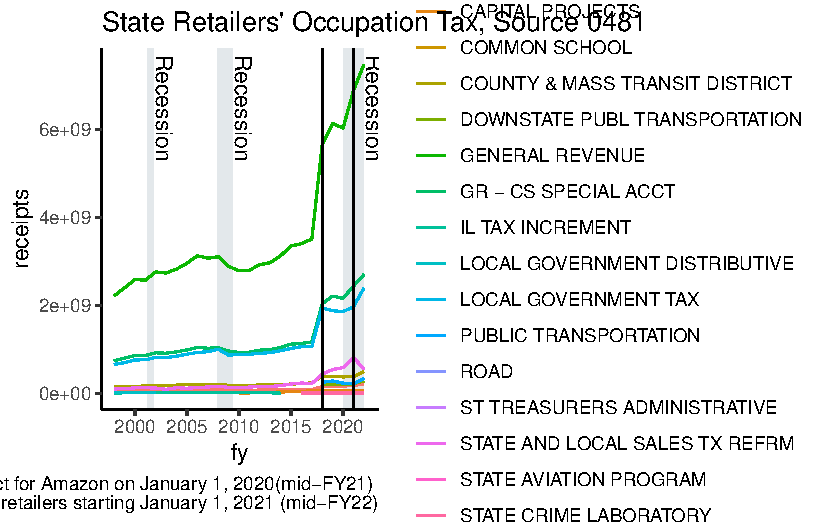
\includegraphics{./FedMoneyReceived_files/figure-pdf/unnamed-chunk-13-1.pdf}

}

\end{figure}

In FY21, \$1.8 billion from the CARES-State CURE went to operations and
grants for programs and services (e.g.~business interruptions, child
care grants, healthcare providers, rent/mortgage assistance, public
health response, etc.), \$1 billion was transferred to other Agencies
for reimbursing pandemic related costs, and \$569 million CARES-ESSER I
funds for K-12 education.

Approximately \$3.08 billion of the ESSER funds had been spent through
FY 2022 (of the \$7.88 billion received from ESSER I, II, and III
received) and in FY 2022 alone, the Illinois School Board for Education
received over \$5 billion from ARPA-ESSER III and spent under \$1
billion of it that fiscal year. These unspent funds do roll over to the
next fiscal year but must be used by 2024. Around \$4 billion remain.

According to the
\href{https://www.isbe.net/Pages/ESSER-Spending-Dashboard.aspx}{ISBE
Spending Dashboard} as of February 2, 2023, \$1.6 billion of ESSER II
and \$1.6 billion of ESSER III funds have been spent so far. ESSER I has
been nearly completely spent, ISBE has spent 79\% of its ESSER II
allocations and has spent 33\% of its ESSER III allocations.

\begin{Shaded}
\begin{Highlighting}[]
\CommentTok{\# all funds through FY22 spent}
\CommentTok{\# Year Spent, Agency received, FF Spending Category }
\FunctionTok{ggplot}\NormalTok{(cure\_exp2022, }
       \FunctionTok{aes}\NormalTok{(}\AttributeTok{y =} \StringTok{\textasciigrave{}}\AttributeTok{FY Expenditures}\StringTok{\textasciigrave{}}\NormalTok{, }\AttributeTok{axis3 =}\NormalTok{ FY\_Spent, }\AttributeTok{axis2 =}\NormalTok{ Agency, }\AttributeTok{axis1=}\NormalTok{FF\_Cat2, }\AttributeTok{label =} \StringTok{"stratum"}\NormalTok{)) }\SpecialCharTok{+}
  \FunctionTok{geom\_flow}\NormalTok{(}\FunctionTok{aes}\NormalTok{(}\AttributeTok{fill =}\NormalTok{ Law), }\AttributeTok{color =} \StringTok{"black"}\NormalTok{, }\AttributeTok{reverse=}\ConstantTok{FALSE}\NormalTok{) }\SpecialCharTok{+}
  \FunctionTok{geom\_stratum}\NormalTok{(}\AttributeTok{reverse=}\ConstantTok{FALSE}\NormalTok{)}\SpecialCharTok{+}
 \CommentTok{\#geom\_text(stat = "stratum", label.strata = TRUE, reverse=FALSE) + }
  \FunctionTok{coord\_flip}\NormalTok{()}\SpecialCharTok{+}
   \FunctionTok{scale\_fill\_brewer}\NormalTok{(}\AttributeTok{palette =} \StringTok{"YlOrRd"}\NormalTok{, }\AttributeTok{direction =} \SpecialCharTok{{-}}\DecValTok{1}\NormalTok{)}\SpecialCharTok{+}
        \FunctionTok{geom\_text}\NormalTok{(}\AttributeTok{stat =} \StringTok{"stratum"}\NormalTok{, }\FunctionTok{aes}\NormalTok{(}\AttributeTok{label =} \FunctionTok{after\_stat}\NormalTok{(stratum)), }\AttributeTok{size =} \DecValTok{2}\NormalTok{, }\AttributeTok{reverse=}\ConstantTok{FALSE}\NormalTok{)}\SpecialCharTok{+}
  \FunctionTok{theme\_void}\NormalTok{() }\SpecialCharTok{+} 
  \FunctionTok{theme}\NormalTok{(}\AttributeTok{legend.position=}\StringTok{"bottom"}\NormalTok{)}\SpecialCharTok{+}
  \FunctionTok{labs}\NormalTok{( }\AttributeTok{title =} \StringTok{"CURE, ESSER, and other Federal Grants = $15.3 Billion Spent FY20{-}FY22"}\NormalTok{, }
        \AttributeTok{subtitle =} \StringTok{"Year Spent, Agency that Spent it \& FF Spending Category"}\NormalTok{)}
\end{Highlighting}
\end{Shaded}

\begin{figure}[H]

{\centering 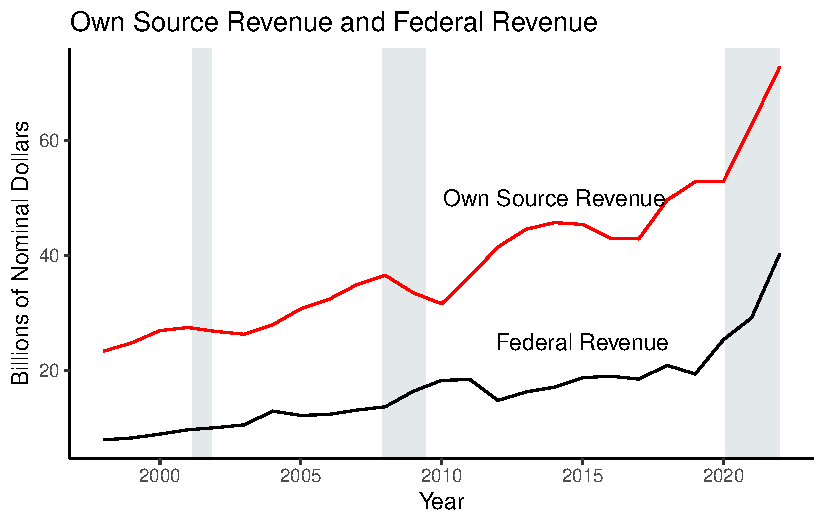
\includegraphics{./FedMoneyReceived_files/figure-pdf/unnamed-chunk-14-1.pdf}

}

\end{figure}

\begin{itemize}
\tightlist
\item
  \$500 million spent in FY2020 (CARES State CURE \& CARES-ESSER I)
\item
  \$3.82 billion spent in FY2021 (CARES State CURE, CRRSA-ESSER
  II,\ldots{} )
\item
  \$11.03 billion spent in FY 2022 (remaining \$0.5 billion CARES-State
  CURE, \$5.2 billion from ARPA-State CURE, \$2 billion from ESSER II \&
  III, plus other funds from federal grants to state agencies).
\end{itemize}

\begin{Shaded}
\begin{Highlighting}[]
\NormalTok{cure\_exp2022 }\SpecialCharTok{\%\textgreater{}\%} 
  \FunctionTok{group\_by}\NormalTok{(}\StringTok{\textasciigrave{}}\AttributeTok{Federal Funds}\StringTok{\textasciigrave{}}\NormalTok{)}\SpecialCharTok{\%\textgreater{}\%} 
  \FunctionTok{summarize}\NormalTok{(}\AttributeTok{Expenditures=}\FunctionTok{sum}\NormalTok{(}\StringTok{\textasciigrave{}}\AttributeTok{FY Expenditures}\StringTok{\textasciigrave{}}\NormalTok{))}
\end{Highlighting}
\end{Shaded}

\begin{verbatim}
# A tibble: 3 x 2
  `Federal Funds` Expenditures
  <chr>                  <dbl>
1 CRF                    3474 
2 Other Fed Rev          6945.
3 SLFRF                  4927 
\end{verbatim}

\begin{Shaded}
\begin{Highlighting}[]
\NormalTok{cure\_exp2022 }\SpecialCharTok{\%\textgreater{}\%} \CommentTok{\#expenditures per year}
  \FunctionTok{group\_by}\NormalTok{(}\StringTok{\textasciigrave{}}\AttributeTok{FY\_Spent}\StringTok{\textasciigrave{}}\NormalTok{)}\SpecialCharTok{\%\textgreater{}\%} 
  \FunctionTok{summarize}\NormalTok{(}\AttributeTok{Expenditures=}\FunctionTok{sum}\NormalTok{(}\StringTok{\textasciigrave{}}\AttributeTok{FY Expenditures}\StringTok{\textasciigrave{}}\NormalTok{))}
\end{Highlighting}
\end{Shaded}

\begin{verbatim}
# A tibble: 3 x 2
  FY_Spent Expenditures
  <fct>           <dbl>
1 2020             498.
2 2021            3817.
3 2022           11031.
\end{verbatim}

\begin{Shaded}
\begin{Highlighting}[]
\NormalTok{cure\_exp2022 }\SpecialCharTok{\%\textgreater{}\%} 
  \FunctionTok{group\_by}\NormalTok{(}\StringTok{\textasciigrave{}}\AttributeTok{FF\_Cat}\StringTok{\textasciigrave{}}\NormalTok{)}\SpecialCharTok{\%\textgreater{}\%} 
  \FunctionTok{summarize}\NormalTok{(}\AttributeTok{Expenditures=}\FunctionTok{sum}\NormalTok{(}\StringTok{\textasciigrave{}}\AttributeTok{FY Expenditures}\StringTok{\textasciigrave{}}\NormalTok{))}
\end{Highlighting}
\end{Shaded}

\begin{verbatim}
# A tibble: 10 x 2
   FF_Cat          Expenditures
   <chr>                  <dbl>
 1 Econ Dev               2921 
 2 Human Services         1868 
 3 K-12                   3082.
 4 Local Transfers         240 
 5 Lost Revenue           1000 
 6 Medicare                705 
 7 Public Health          1166 
 8 Public Safety           485 
 9 Reimbursements         1179 
10 UI Fund                2700 
\end{verbatim}

\begin{Shaded}
\begin{Highlighting}[]
\NormalTok{cure\_exp2022 }\SpecialCharTok{\%\textgreater{}\%} 
  \FunctionTok{group\_by}\NormalTok{(Law)}\SpecialCharTok{\%\textgreater{}\%} 
  \FunctionTok{summarize}\NormalTok{(}\AttributeTok{Expenditures=}\FunctionTok{sum}\NormalTok{(}\StringTok{\textasciigrave{}}\AttributeTok{FY Expenditures}\StringTok{\textasciigrave{}}\NormalTok{))}
\end{Highlighting}
\end{Shaded}

\begin{verbatim}
# A tibble: 3 x 2
  Law   Expenditures
  <chr>        <dbl>
1 ARPA         7798.
2 CARES        4305.
3 CRRSA        3243.
\end{verbatim}

\begin{Shaded}
\begin{Highlighting}[]
\NormalTok{cure\_exp2022 }\SpecialCharTok{\%\textgreater{}\%} 
  \FunctionTok{group\_by}\NormalTok{(Law, FY\_Spent, FF\_Cat2)}\SpecialCharTok{\%\textgreater{}\%} 
  \FunctionTok{summarize}\NormalTok{(}\AttributeTok{Expenditures=}\FunctionTok{sum}\NormalTok{(}\StringTok{\textasciigrave{}}\AttributeTok{FY Expenditures}\StringTok{\textasciigrave{}}\NormalTok{)) }\SpecialCharTok{\%\textgreater{}\%}
  \FunctionTok{pivot\_wider}\NormalTok{(}\AttributeTok{names\_from =}\NormalTok{ FY\_Spent, }\AttributeTok{values\_from =}\NormalTok{ Expenditures) }
\end{Highlighting}
\end{Shaded}

\begin{verbatim}
# A tibble: 17 x 5
# Groups:   Law [3]
   Law   FF_Cat2                `2022` `2020` `2021`
   <chr> <chr>                   <dbl>  <dbl>  <dbl>
 1 ARPA  Econ Dev                1694     NA     NA 
 2 ARPA  Human Services          1276     NA     NA 
 3 ARPA  K-12                     838.    NA     NA 
 4 ARPA  Lost Revenue            1000     NA     NA 
 5 ARPA  Public Health & Safety   290     NA     NA 
 6 ARPA  UI Fund                 2700     NA     NA 
 7 CARES K-12                      60    128.   376.
 8 CARES Public Health & Safety   267    370     60 
 9 CARES Econ Dev                  NA     NA    660 
10 CARES Human Services            NA     NA    260 
11 CARES Local Transfers           19     NA    221 
12 CARES Medicare                  53     NA    652 
13 CARES Reimbursements           174     NA   1005 
14 CRRSA K-12                    1097.    NA    584.
15 CRRSA Econ Dev                 567     NA     NA 
16 CRRSA Human Services           332     NA     NA 
17 CRRSA Public Health & Safety   664     NA     NA 
\end{verbatim}

\begin{Shaded}
\begin{Highlighting}[]
\NormalTok{cure\_exp2022 }\SpecialCharTok{\%\textgreater{}\%} 
  \FunctionTok{group\_by}\NormalTok{(Law, FY\_Received)}\SpecialCharTok{\%\textgreater{}\%} 
  \FunctionTok{summarize}\NormalTok{(}\AttributeTok{Expenditures=}\FunctionTok{sum}\NormalTok{(}\StringTok{\textasciigrave{}}\AttributeTok{FY Expenditures}\StringTok{\textasciigrave{}}\NormalTok{)) }\SpecialCharTok{\%\textgreater{}\%}
  \FunctionTok{pivot\_wider}\NormalTok{(}\AttributeTok{names\_from =}\NormalTok{ Law, }\AttributeTok{values\_from =}\NormalTok{ Expenditures) }\SpecialCharTok{\%\textgreater{}\%} \FunctionTok{arrange}\NormalTok{(FY\_Received)}
\end{Highlighting}
\end{Shaded}

\begin{verbatim}
# A tibble: 3 x 4
  FY_Received  ARPA CARES CRRSA
  <fct>       <dbl> <dbl> <dbl>
1 2020          NA  4305.   NA 
2 2021          NA    NA   584.
3 2022        7798.   NA  2660.
\end{verbatim}

\begin{Shaded}
\begin{Highlighting}[]
\NormalTok{cure\_exp2022 }\SpecialCharTok{\%\textgreater{}\%} 
  \FunctionTok{group\_by}\NormalTok{(Law, FY\_Spent)}\SpecialCharTok{\%\textgreater{}\%} 
  \FunctionTok{summarize}\NormalTok{(}\AttributeTok{Expenditures=}\FunctionTok{sum}\NormalTok{(}\StringTok{\textasciigrave{}}\AttributeTok{FY Expenditures}\StringTok{\textasciigrave{}}\NormalTok{)) }\SpecialCharTok{\%\textgreater{}\%}
  \FunctionTok{pivot\_wider}\NormalTok{(}\AttributeTok{names\_from =}\NormalTok{ Law, }\AttributeTok{values\_from =}\NormalTok{ Expenditures) }\SpecialCharTok{\%\textgreater{}\%}
  \FunctionTok{arrange}\NormalTok{(FY\_Spent)}
\end{Highlighting}
\end{Shaded}

\begin{verbatim}
# A tibble: 3 x 4
  FY_Spent  ARPA CARES CRRSA
  <fct>    <dbl> <dbl> <dbl>
1 2020       NA   498.   NA 
2 2021       NA  3234.  584.
3 2022     7798.  573  2660.
\end{verbatim}

\hypertarget{state-cure-expenditures-with-fy2023-and-beyond-allocations}{%
\subsection{State CURE Expenditures with FY2023 and beyond
allocations}\label{state-cure-expenditures-with-fy2023-and-beyond-allocations}}

Graphs below include how money has been spent through FY22 with unspent
funds labeled as \texttt{FY2023+}. Only State CURE funds are included.
ESSER and other federal grants to state departments are excluded. Funds
may be used for expenses obligated through December 31, 2024 and
expended by December 31, 2026.

An additional \$254 million is expected to come to Illinois from the
Coronavirus Capital Projects Fund to be used for Connect Illinois
broadband projects (GOMB December 2022 LBOC report). This has been left
out of all graphs and summaries.\\

\begin{itemize}
\item
  \$3.54 Billion received in FY20 for State Fiscal Recovery Fund (SFRF)+
  \$11.8 billion received in FY22 = \$15.3 billion total expenditures
  and allocations included in this image.
\item
  Around \$10.8 billion has gone into the State CURE fund (Coronavirus
  Relief Funds (CRF) and SFRF into the State CURE fund) and another
  \$4.5 billion was received by State Departments (mostly ISBE for K-12
  )
\item
  So far, over \$13 billion has been spent.

  \begin{itemize}
  \item
    \$2.7 billion was spent in FY21 and \$8.5 Billion was spent in FY22.
  \item
    The remaining \$2 Billion State CURE funds have been fully allocated
    and some have been spent already in FY23 (\$500 million transferred
    to General Revenue for ``Lost Revenue'' during COVID disruption,
    remaining dollars on programs and services).
  \end{itemize}
\end{itemize}

\begin{Shaded}
\begin{Highlighting}[]
\CommentTok{\# cure\_exp2023 keeps State CURE only!}
\NormalTok{cure\_exp2023 }\OtherTok{\textless{}{-}}\NormalTok{ cure\_exp }\SpecialCharTok{\%\textgreater{}\%}
  \FunctionTok{filter}\NormalTok{(State\_local }\SpecialCharTok{==} \StringTok{"State CURE"}\NormalTok{) }\SpecialCharTok{\%\textgreater{}\%}
  \FunctionTok{mutate}\NormalTok{(}\AttributeTok{Law =} \FunctionTok{factor}\NormalTok{(Law, }\AttributeTok{levels =} \FunctionTok{c}\NormalTok{(}\StringTok{"CARES"}\NormalTok{, }\StringTok{"ARPA"}\NormalTok{)),}
         \AttributeTok{FY\_Spent =} \FunctionTok{factor}\NormalTok{(FY\_Spent, }\AttributeTok{levels =} \FunctionTok{c}\NormalTok{(}\StringTok{"2020"}\NormalTok{, }\StringTok{"2021"}\NormalTok{, }\StringTok{"2022"}\NormalTok{, }\StringTok{"2023"}\NormalTok{)),}
         \AttributeTok{FY\_Received =} \FunctionTok{factor}\NormalTok{(FY\_Received, }\AttributeTok{levels =} \FunctionTok{c}\NormalTok{(}\StringTok{"2020"}\NormalTok{, }\StringTok{"2021"}\NormalTok{, }\StringTok{"2022"}\NormalTok{)),}
        \AttributeTok{FF\_Cat =} \FunctionTok{factor}\NormalTok{(FF\_Cat, }\AttributeTok{levels =} \FunctionTok{c}\NormalTok{(}\StringTok{"Econ Dev"}\NormalTok{, }\StringTok{"Human Services"}\NormalTok{, }\StringTok{"K{-}12"}\NormalTok{, }\StringTok{"Local Transfers"}\NormalTok{, }\StringTok{"Public Health"}\NormalTok{, }\StringTok{"Medicare"}\NormalTok{, }\StringTok{"Public Safety"}\NormalTok{, }\StringTok{"Transportation"}\NormalTok{, }\StringTok{"Reimbursements"}\NormalTok{,  }\StringTok{"UI Fund"}\NormalTok{, }\StringTok{"Capital Projects"}\NormalTok{, }\StringTok{"Lost Revenue"}\NormalTok{, }\StringTok{"FY23+"}\NormalTok{)),}
        \AttributeTok{FF\_Cat2 =} \FunctionTok{factor}\NormalTok{(FF\_Cat2, }\AttributeTok{levels =} \FunctionTok{c}\NormalTok{(}\StringTok{"Econ Dev"}\NormalTok{, }\StringTok{"Human Services"}\NormalTok{, }\StringTok{"K{-}12"}\NormalTok{, }\StringTok{"Local Transfers"}\NormalTok{, }\StringTok{"Public Health \& Safety"}\NormalTok{, }\StringTok{"Medicaid"}\NormalTok{, }\StringTok{"Medicare"}\NormalTok{, }\StringTok{"Transportation"}\NormalTok{, }\StringTok{"Reimbursements"}\NormalTok{, }\StringTok{"UI Fund"}\NormalTok{, }\StringTok{"Capital Projects"}\NormalTok{, }\StringTok{"Lost Revenue"}\NormalTok{,}\StringTok{"FY23+"}\NormalTok{))}
\NormalTok{      )}


\NormalTok{cure\_exp2023 }\OtherTok{\textless{}{-}}\NormalTok{ cure\_exp2023 }\SpecialCharTok{\%\textgreater{}\%} 
  \FunctionTok{group\_by}\NormalTok{(State\_local) }\SpecialCharTok{\%\textgreater{}\%} 
  \FunctionTok{mutate}\NormalTok{(}\AttributeTok{pct =} \StringTok{\textasciigrave{}}\AttributeTok{FY Expenditures}\StringTok{\textasciigrave{}} \SpecialCharTok{/} \FunctionTok{sum}\NormalTok{(}\StringTok{\textasciigrave{}}\AttributeTok{FY Expenditures}\StringTok{\textasciigrave{}}\NormalTok{))}

\NormalTok{cure\_exp2023 }\SpecialCharTok{\%\textgreater{}\%} 
  \FunctionTok{filter}\NormalTok{(State\_local }\SpecialCharTok{==} \StringTok{"State CURE"}\NormalTok{)}\SpecialCharTok{\%\textgreater{}\%} 
  \FunctionTok{summarize}\NormalTok{(}\AttributeTok{sum=}\FunctionTok{sum}\NormalTok{(}\StringTok{\textasciigrave{}}\AttributeTok{FY Expenditures}\StringTok{\textasciigrave{}}\NormalTok{))}
\end{Highlighting}
\end{Shaded}

\begin{verbatim}
# A tibble: 1 x 2
  State_local   sum
  <chr>       <dbl>
1 State CURE  11647
\end{verbatim}

\begin{Shaded}
\begin{Highlighting}[]
\NormalTok{cure\_exp2023 }\SpecialCharTok{\%\textgreater{}\%} 
  \FunctionTok{filter}\NormalTok{(State\_local }\SpecialCharTok{==} \StringTok{"State CURE"}\NormalTok{) }\SpecialCharTok{\%\textgreater{}\%}
  \FunctionTok{ggplot}\NormalTok{(}\FunctionTok{aes}\NormalTok{(}\AttributeTok{y =}\NormalTok{ pct, }
             \AttributeTok{axis4 =}\NormalTok{ FY\_Received, }
             \AttributeTok{axis3 =}\NormalTok{ Agency,  }
             \AttributeTok{axis2 =}\NormalTok{ FY\_Spent, }
             \AttributeTok{axis1 =}\NormalTok{ FF\_Cat)) }\SpecialCharTok{+}
  \FunctionTok{geom\_flow}\NormalTok{(}\FunctionTok{aes}\NormalTok{(}\AttributeTok{fill =}\NormalTok{ Law), }\AttributeTok{color =} \StringTok{"black"}\NormalTok{, }\AttributeTok{reverse=}\ConstantTok{FALSE}\NormalTok{) }\SpecialCharTok{+}
  \FunctionTok{geom\_stratum}\NormalTok{(}\AttributeTok{reverse=}\ConstantTok{FALSE}\NormalTok{)}\SpecialCharTok{+}
  \FunctionTok{scale\_fill\_brewer}\NormalTok{(}\AttributeTok{palette =} \StringTok{"YlOrRd"}\NormalTok{, }\AttributeTok{direction =} \SpecialCharTok{{-}}\DecValTok{1}\NormalTok{)}\SpecialCharTok{+}
  \FunctionTok{coord\_flip}\NormalTok{()}\SpecialCharTok{+}
  \FunctionTok{theme\_void}\NormalTok{() }\SpecialCharTok{+} 
  \FunctionTok{theme}\NormalTok{(}\AttributeTok{legend.position=}\StringTok{"bottom"}\NormalTok{)}\SpecialCharTok{+}
 \CommentTok{\# geom\_text(stat = "stratum", aes(label = after\_stat(stratum)), size = 2, reverse=FALSE) +}
  \FunctionTok{geom\_text}\NormalTok{(}\FunctionTok{aes}\NormalTok{(}\AttributeTok{label =} \FunctionTok{paste0}\NormalTok{(..stratum.., }\StringTok{"}\SpecialCharTok{\textbackslash{}n}\StringTok{"}\NormalTok{, scales}\SpecialCharTok{::}\FunctionTok{percent}\NormalTok{(..count.., }\AttributeTok{accuracy =}\NormalTok{ .}\DecValTok{1}\NormalTok{))), }\AttributeTok{stat =} \StringTok{"stratum"}\NormalTok{, }\AttributeTok{reverse=}\ConstantTok{FALSE}\NormalTok{, }\AttributeTok{size=}\DecValTok{2}\NormalTok{) }\SpecialCharTok{+}

 \CommentTok{\# geom\_text(stat = "stratum", aes(label = scales::dollar(after\_stat(stratum),accuracy =0.01)), size = 2, nudge\_x = 0.4) +}

  \FunctionTok{labs}\NormalTok{(}\AttributeTok{title =} \StringTok{"Expenditures \& Allocations of State CURE fund = 11.6 Billion"}\NormalTok{, }
  \AttributeTok{subtitle =} \StringTok{"Year Received by State Department, Year Spent, and Expenditure Purpose"}\NormalTok{, }
  \AttributeTok{caption =} \StringTok{"Expenditures occured during FY20, FY21 and FY22. }
\StringTok{       Additional funds will continue to be spent in FY23{-}FY26."}\NormalTok{)}
\end{Highlighting}
\end{Shaded}

\begin{figure}[H]

{\centering 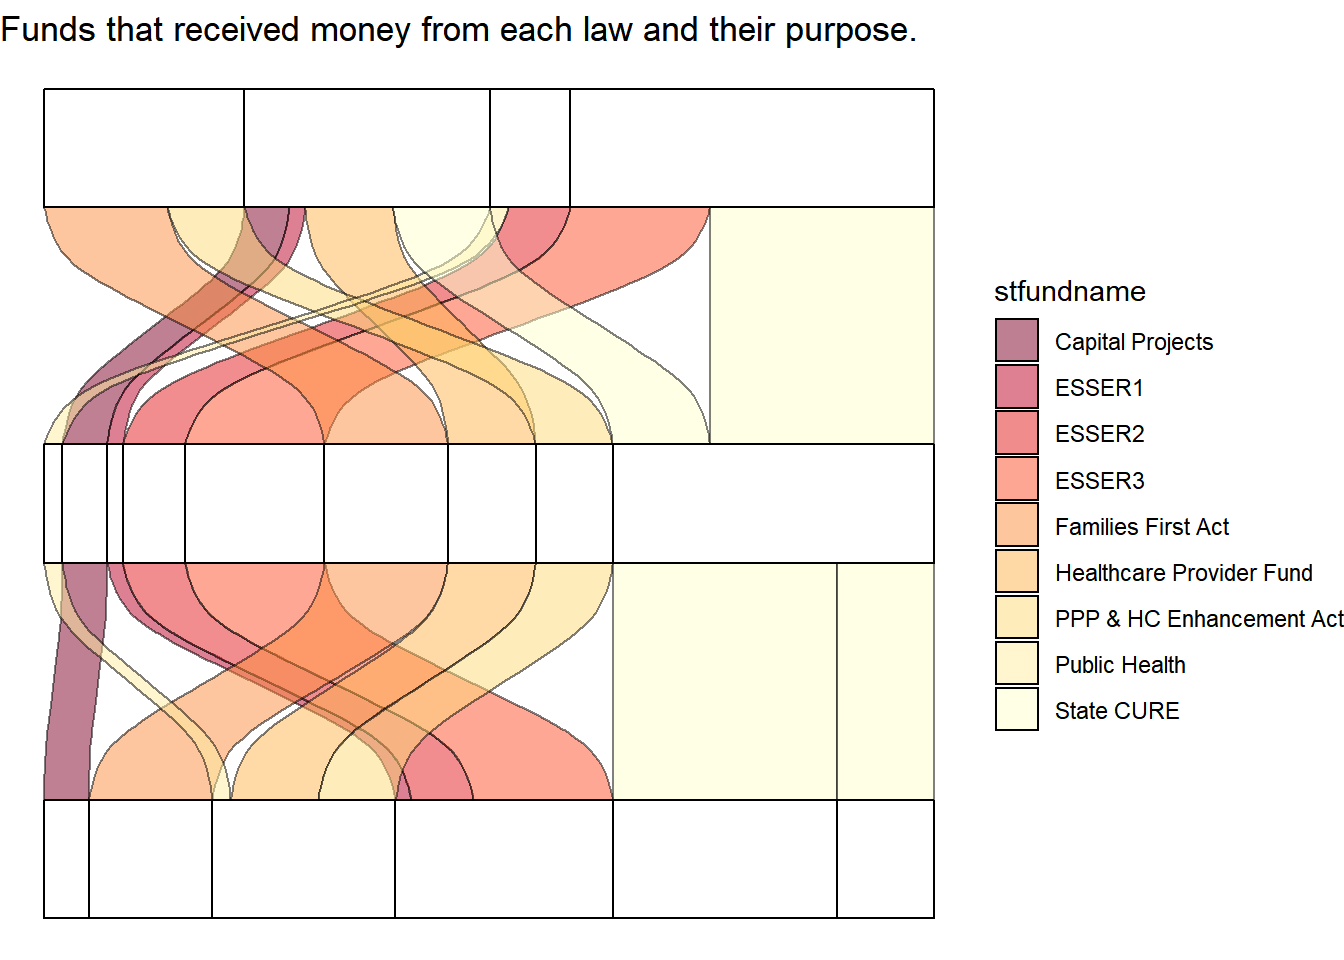
\includegraphics{./FedMoneyReceived_files/figure-pdf/unnamed-chunk-17-1.pdf}

}

\end{figure}

\begin{Shaded}
\begin{Highlighting}[]
\NormalTok{cure\_exp2023 }\SpecialCharTok{\%\textgreater{}\%} 
  \FunctionTok{filter}\NormalTok{(State\_local }\SpecialCharTok{==} \StringTok{"State CURE"}\NormalTok{) }\SpecialCharTok{\%\textgreater{}\%}
  \FunctionTok{ggplot}\NormalTok{(}\FunctionTok{aes}\NormalTok{(}\AttributeTok{y =} \FunctionTok{round}\NormalTok{(}\StringTok{\textasciigrave{}}\AttributeTok{FY Expenditures}\StringTok{\textasciigrave{}}\NormalTok{, }\AttributeTok{digits=}\DecValTok{2}\NormalTok{), }
             \AttributeTok{axis4 =}\NormalTok{ FY\_Received, }
             \AttributeTok{axis3 =}\NormalTok{ Agency\_grouped,  }
             \AttributeTok{axis2 =}\NormalTok{ FY\_Spent, }
             \AttributeTok{axis1 =}\NormalTok{ FF\_Cat2)) }\SpecialCharTok{+}
  \FunctionTok{geom\_flow}\NormalTok{(}\FunctionTok{aes}\NormalTok{(}\AttributeTok{fill =}\NormalTok{ Law), }\AttributeTok{color =} \StringTok{"black"}\NormalTok{, }\AttributeTok{reverse=}\ConstantTok{FALSE}\NormalTok{) }\SpecialCharTok{+}
  \FunctionTok{geom\_stratum}\NormalTok{(}\AttributeTok{reverse=}\ConstantTok{FALSE}\NormalTok{)}\SpecialCharTok{+}
  \FunctionTok{scale\_fill\_brewer}\NormalTok{(}\AttributeTok{palette =} \StringTok{"YlOrRd"}\NormalTok{, }\AttributeTok{direction =} \SpecialCharTok{{-}}\DecValTok{1}\NormalTok{)}\SpecialCharTok{+}
  \FunctionTok{coord\_flip}\NormalTok{()}\SpecialCharTok{+}
  \FunctionTok{theme\_void}\NormalTok{() }\SpecialCharTok{+} 
  \FunctionTok{theme}\NormalTok{(}\AttributeTok{legend.position=}\StringTok{"bottom"}\NormalTok{)}\SpecialCharTok{+}
 \FunctionTok{geom\_text}\NormalTok{(}\AttributeTok{stat =} \StringTok{"stratum"}\NormalTok{, }\FunctionTok{aes}\NormalTok{(}\AttributeTok{label =} \FunctionTok{after\_stat}\NormalTok{(stratum)), }\AttributeTok{size =} \DecValTok{2}\NormalTok{, }\AttributeTok{reverse=}\ConstantTok{FALSE}\NormalTok{) }\SpecialCharTok{+}
\CommentTok{\#  geom\_text(aes(label = paste0(..stratum.., "\textbackslash{}n", scales::percent(..count.., accuracy = .1))), stat = "stratum") +}

 \CommentTok{\# geom\_text(stat = "stratum", aes(label = scales::dollar(after\_stat(stratum),accuracy =0.01)), size = 2, nudge\_x = 0.4) +}

  \FunctionTok{labs}\NormalTok{(}\AttributeTok{title =} \StringTok{"(Same as above but without percentages)Expenditures using State CURE funds"}\NormalTok{, }
  \AttributeTok{subtitle =} \StringTok{"Year Received by State Department, Year Spent, and how it was spent so far"}\NormalTok{, }\AttributeTok{caption =} \StringTok{"Expenditures occured during FY21 and FY22. }
\StringTok{       Additional funds will continue to be spent in FY23{-}FY26."}\NormalTok{)}
\end{Highlighting}
\end{Shaded}

\begin{figure}[H]

{\centering 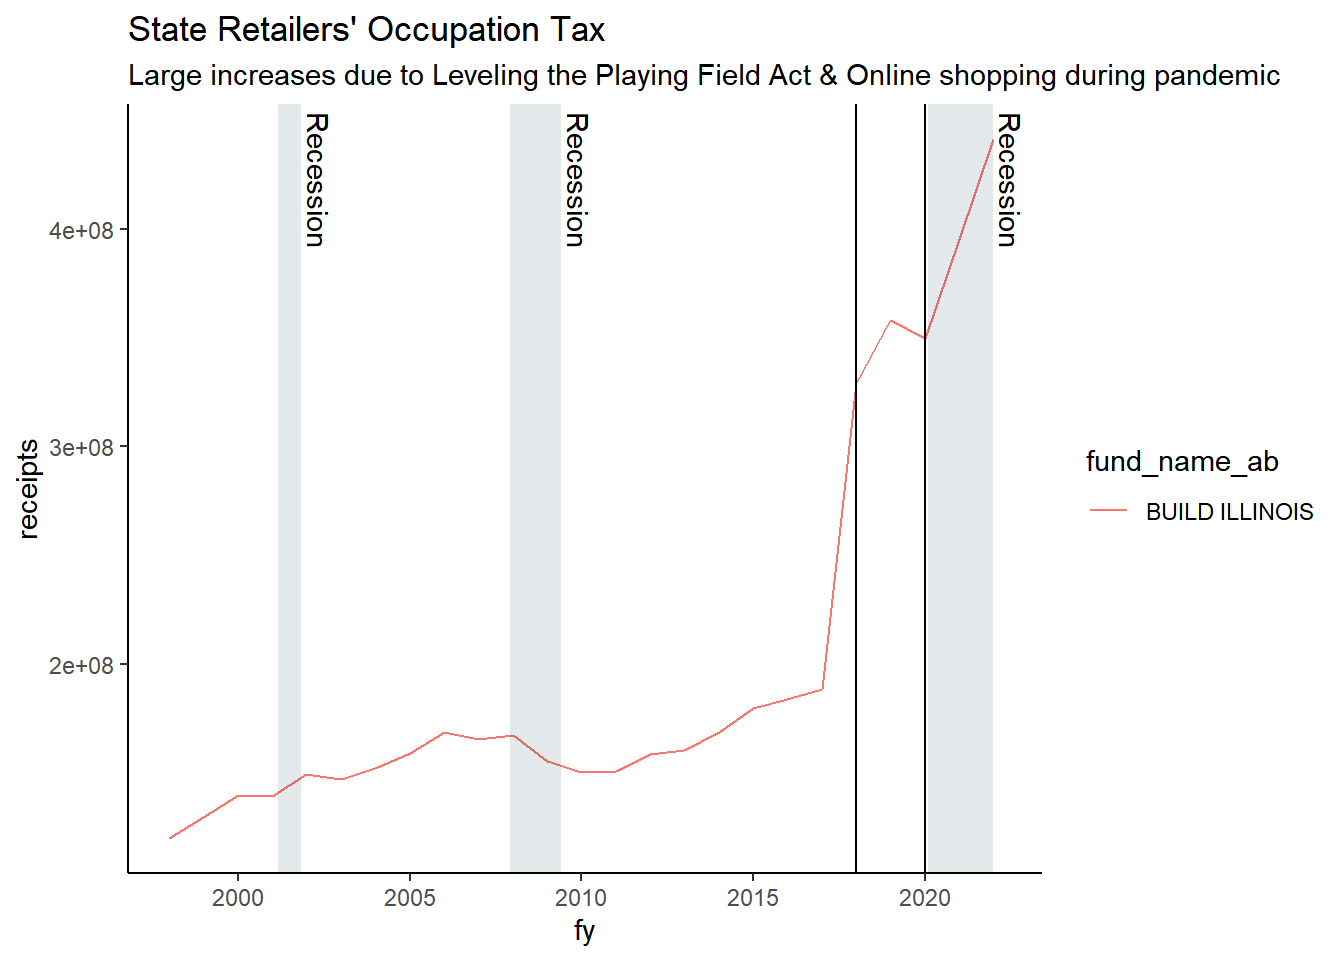
\includegraphics{./FedMoneyReceived_files/figure-pdf/unnamed-chunk-17-2.pdf}

}

\end{figure}

\begin{Shaded}
\begin{Highlighting}[]
\CommentTok{\#5 levels with labels}
\FunctionTok{ggplot}\NormalTok{(cure\_exp2023, }
       \FunctionTok{aes}\NormalTok{(}\AttributeTok{y =} \StringTok{\textasciigrave{}}\AttributeTok{FY Expenditures}\StringTok{\textasciigrave{}}\NormalTok{,  }
           \AttributeTok{axis6 =} \StringTok{\textasciigrave{}}\AttributeTok{Federal Funds}\StringTok{\textasciigrave{}}\NormalTok{, }
           \AttributeTok{axis5=}\NormalTok{State\_local2, }
      \CommentTok{\#     axis4 = \textasciigrave{}FY\_Received\textasciigrave{},}
           \AttributeTok{axis3 =}\NormalTok{ Agency\_grouped, }
           \AttributeTok{axis2 =}\NormalTok{ FY\_Spent, }\AttributeTok{axis1=}\NormalTok{FF\_Cat2, }\AttributeTok{label =} \StringTok{"stratum"}\NormalTok{)) }\SpecialCharTok{+}
  \FunctionTok{geom\_flow}\NormalTok{(}\FunctionTok{aes}\NormalTok{(}\AttributeTok{fill =}\NormalTok{ Law), }\AttributeTok{color =} \StringTok{"black"}\NormalTok{, }\AttributeTok{reverse=}\ConstantTok{FALSE}\NormalTok{) }\SpecialCharTok{+}
  \FunctionTok{geom\_stratum}\NormalTok{(}\AttributeTok{reverse=}\ConstantTok{FALSE}\NormalTok{)}\SpecialCharTok{+}  \FunctionTok{coord\_flip}\NormalTok{()}\SpecialCharTok{+}
  \FunctionTok{scale\_fill\_brewer}\NormalTok{(}\AttributeTok{palette =} \StringTok{"YlOrRd"}\NormalTok{, }\AttributeTok{direction =} \SpecialCharTok{{-}}\DecValTok{1}\NormalTok{)}\SpecialCharTok{+}
  \FunctionTok{theme\_void}\NormalTok{() }\SpecialCharTok{+} 
  \FunctionTok{theme}\NormalTok{(}\AttributeTok{legend.position =} \StringTok{"bottom"}\NormalTok{)}\SpecialCharTok{+}
  \FunctionTok{geom\_text}\NormalTok{(}\AttributeTok{stat =} \StringTok{"stratum"}\NormalTok{, }\FunctionTok{aes}\NormalTok{(}\AttributeTok{label =} \FunctionTok{after\_stat}\NormalTok{(stratum)), }\AttributeTok{size =} \DecValTok{2}\NormalTok{, }\AttributeTok{reverse=}\ConstantTok{FALSE}\NormalTok{) }\SpecialCharTok{+} 
  \FunctionTok{labs}\NormalTok{(}\AttributeTok{title =} \StringTok{"$11.6 Billion in Expenditures and Allocations from Federal Stimulus Packages"}\NormalTok{,}
       \AttributeTok{subtitle =} \StringTok{"Only State CURE funds are included in image"}\NormalTok{)}
\end{Highlighting}
\end{Shaded}

\begin{figure}[H]

{\centering 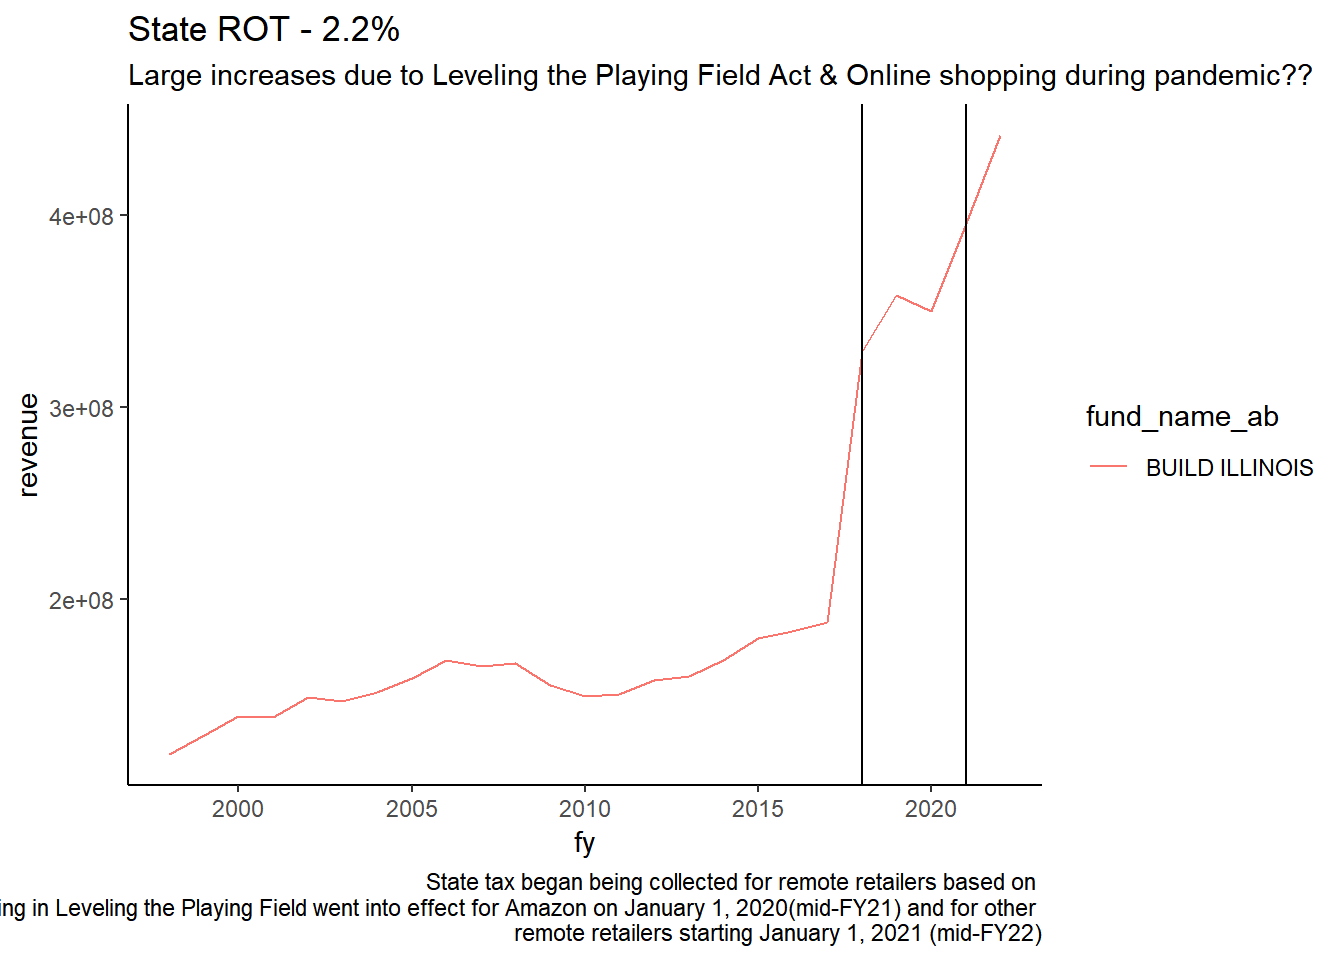
\includegraphics{./FedMoneyReceived_files/figure-pdf/unnamed-chunk-17-3.pdf}

}

\end{figure}

\begin{Shaded}
\begin{Highlighting}[]
\CommentTok{\#5 levels with labels}
\FunctionTok{ggplot}\NormalTok{(cure\_exp2023, }
       \FunctionTok{aes}\NormalTok{(}\AttributeTok{y =} \StringTok{\textasciigrave{}}\AttributeTok{FY Expenditures}\StringTok{\textasciigrave{}}\NormalTok{,  }
           \AttributeTok{axis6 =} \StringTok{\textasciigrave{}}\AttributeTok{Federal Funds}\StringTok{\textasciigrave{}}\NormalTok{, }\AttributeTok{axis5=}\NormalTok{State\_local2, }
         \AttributeTok{axis3 =}\NormalTok{ Agency\_grouped, }
           \AttributeTok{axis2 =}\NormalTok{ FY\_Spent, }\AttributeTok{axis1=}\NormalTok{FF\_Cat2, }\AttributeTok{label =} \StringTok{"stratum"}\NormalTok{)) }\SpecialCharTok{+}
  \FunctionTok{geom\_flow}\NormalTok{(}\FunctionTok{aes}\NormalTok{(}\AttributeTok{fill =}\NormalTok{ FY\_Spent), }\AttributeTok{color =} \StringTok{"black"}\NormalTok{, }\AttributeTok{reverse=}\ConstantTok{FALSE}\NormalTok{) }\SpecialCharTok{+}
  \FunctionTok{geom\_stratum}\NormalTok{(}\AttributeTok{reverse=}\ConstantTok{FALSE}\NormalTok{)}\SpecialCharTok{+}  \FunctionTok{coord\_flip}\NormalTok{()}\SpecialCharTok{+}
  \FunctionTok{scale\_fill\_brewer}\NormalTok{(}\AttributeTok{palette =} \StringTok{"YlOrRd"}\NormalTok{, }\AttributeTok{direction =} \SpecialCharTok{{-}}\DecValTok{1}\NormalTok{)}\SpecialCharTok{+}
  \FunctionTok{theme\_void}\NormalTok{() }\SpecialCharTok{+} 
  \FunctionTok{theme}\NormalTok{(}\AttributeTok{legend.position =} \StringTok{"bottom"}\NormalTok{)}\SpecialCharTok{+}
  \FunctionTok{geom\_text}\NormalTok{(}\AttributeTok{stat =} \StringTok{"stratum"}\NormalTok{, }\FunctionTok{aes}\NormalTok{(}\AttributeTok{label =} \FunctionTok{after\_stat}\NormalTok{(stratum)), }\AttributeTok{size =} \DecValTok{2}\NormalTok{, }\AttributeTok{reverse=}\ConstantTok{FALSE}\NormalTok{) }\SpecialCharTok{+} 
  \FunctionTok{labs}\NormalTok{(}\AttributeTok{title =} \StringTok{"$11.6 Billion in Expenditures and Allocations from Federal Stimulus Packages"}\NormalTok{,}
       \AttributeTok{subtitle =} \StringTok{"Only State CURE funds are included in image"}\NormalTok{)}
\end{Highlighting}
\end{Shaded}

\begin{figure}[H]

{\centering 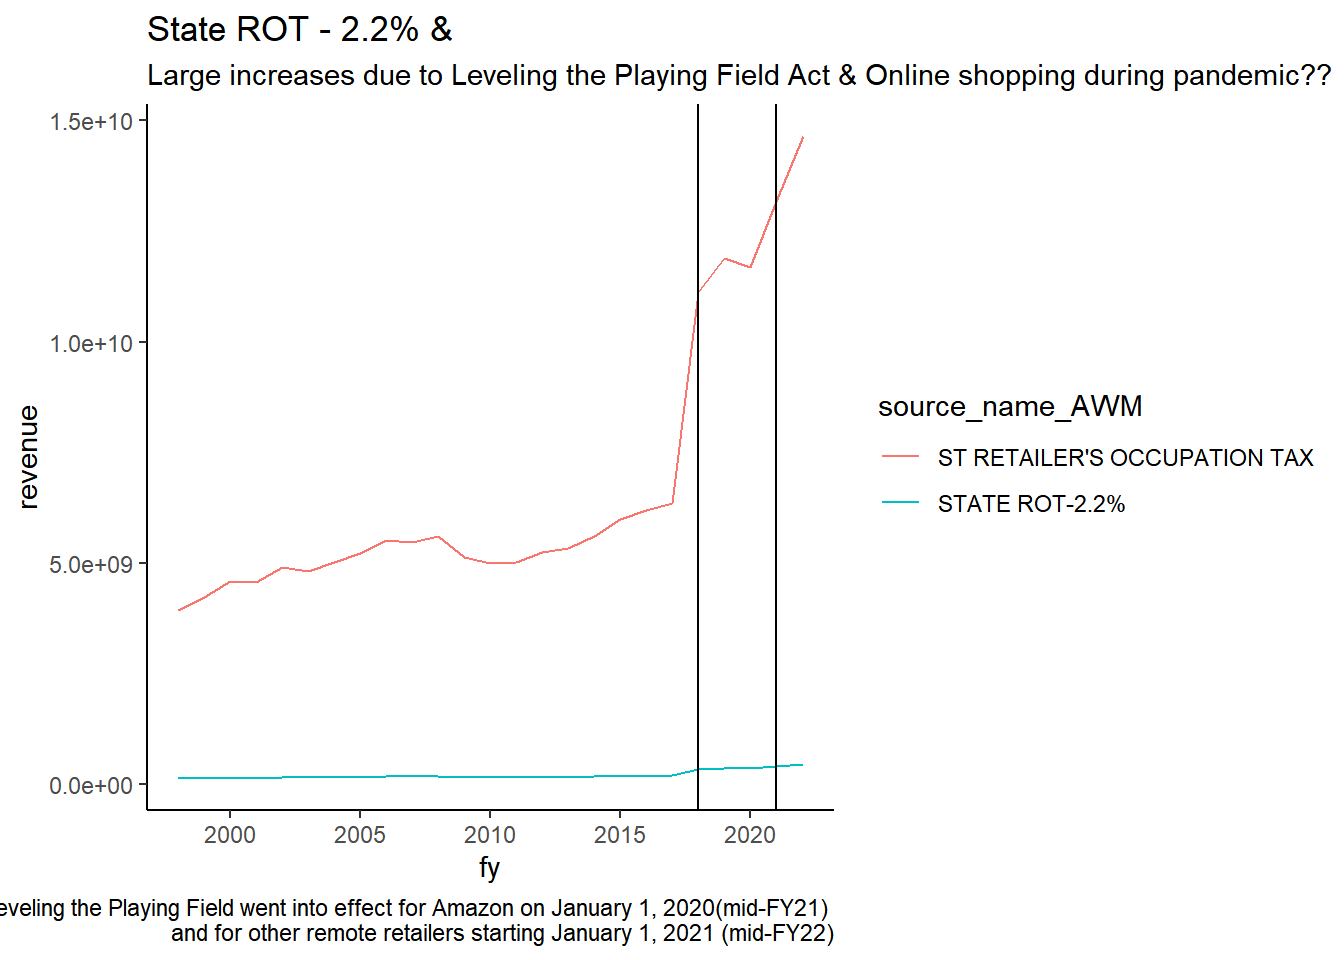
\includegraphics{./FedMoneyReceived_files/figure-pdf/unnamed-chunk-17-4.pdf}

}

\end{figure}

\begin{Shaded}
\begin{Highlighting}[]
\CommentTok{\#4 levels with labels}


\CommentTok{\# State CURE funds only}
\NormalTok{cure\_exp2023 }\SpecialCharTok{\%\textgreater{}\%} 
  \FunctionTok{filter}\NormalTok{(State\_local2 }\SpecialCharTok{==} \StringTok{"State"}\NormalTok{) }\SpecialCharTok{\%\textgreater{}\%}
\FunctionTok{ggplot}\NormalTok{(}\FunctionTok{aes}\NormalTok{(}\AttributeTok{y =} \StringTok{\textasciigrave{}}\AttributeTok{FY Expenditures}\StringTok{\textasciigrave{}}\NormalTok{, }
           \AttributeTok{axis4 =} \StringTok{\textasciigrave{}}\AttributeTok{Federal Funds}\StringTok{\textasciigrave{}}\NormalTok{,  }\AttributeTok{axis3 =}\NormalTok{ Agency\_grouped, }
           \AttributeTok{axis2 =}\NormalTok{ FY\_Spent, }\AttributeTok{axis1=}\NormalTok{FF\_Cat2, }\AttributeTok{label =} \StringTok{"stratum"}\NormalTok{)) }\SpecialCharTok{+}
  \FunctionTok{geom\_flow}\NormalTok{(}\FunctionTok{aes}\NormalTok{(}\AttributeTok{fill =}\NormalTok{ Law), }\AttributeTok{color =} \StringTok{"black"}\NormalTok{, }\AttributeTok{reverse=}\ConstantTok{FALSE}\NormalTok{) }\SpecialCharTok{+}
  \FunctionTok{geom\_stratum}\NormalTok{(}\AttributeTok{reverse=}\ConstantTok{FALSE}\NormalTok{)}\SpecialCharTok{+}  \FunctionTok{coord\_flip}\NormalTok{()}\SpecialCharTok{+}
   \FunctionTok{scale\_fill\_brewer}\NormalTok{(}\AttributeTok{palette =} \StringTok{"YlOrRd"}\NormalTok{, }\AttributeTok{direction =} \SpecialCharTok{{-}}\DecValTok{1}\NormalTok{)}\SpecialCharTok{+}
  \FunctionTok{theme\_void}\NormalTok{() }\SpecialCharTok{+} 
  \FunctionTok{theme}\NormalTok{(}\AttributeTok{legend.position =} \StringTok{"bottom"}\NormalTok{)}\SpecialCharTok{+}
        \FunctionTok{geom\_text}\NormalTok{(}\AttributeTok{stat =} \StringTok{"stratum"}\NormalTok{, }\FunctionTok{aes}\NormalTok{(}\AttributeTok{label =} \FunctionTok{after\_stat}\NormalTok{(stratum)), }\AttributeTok{size =} \DecValTok{2}\NormalTok{, }\AttributeTok{reverse=}\ConstantTok{FALSE}\NormalTok{) }\SpecialCharTok{+} 
  \FunctionTok{labs}\NormalTok{(}\AttributeTok{title =} \StringTok{"$11.6 Billion in Expenditures and Allocations from Federal Stimulus Packages"}\NormalTok{, }
          \AttributeTok{caption =}\StringTok{" Expenditures and Allocations match State CURE revenues from CARES and ARP Acts."}\NormalTok{)}
\end{Highlighting}
\end{Shaded}

\begin{figure}[H]

{\centering \includegraphics{./FedMoneyReceived_files/figure-pdf/unnamed-chunk-17-5.pdf}

}

\end{figure}

\begin{Shaded}
\begin{Highlighting}[]
\NormalTok{cure\_exp2023 }\SpecialCharTok{\%\textgreater{}\%} 
  \FunctionTok{filter}\NormalTok{(State\_local }\SpecialCharTok{==} \StringTok{"State CURE"}\NormalTok{) }\SpecialCharTok{\%\textgreater{}\%} \CommentTok{\# for only state CURE funds}
  \FunctionTok{ggplot}\NormalTok{(}\FunctionTok{aes}\NormalTok{(}\AttributeTok{y =} \StringTok{\textasciigrave{}}\AttributeTok{FY Expenditures}\StringTok{\textasciigrave{}}\NormalTok{, }\AttributeTok{axis4 =}\NormalTok{ FY\_Received, }\AttributeTok{axis3 =} \StringTok{\textasciigrave{}}\AttributeTok{Agency}\StringTok{\textasciigrave{}}\NormalTok{,  }
             \AttributeTok{axis2 =}\NormalTok{ FY\_Spent, }\AttributeTok{axis1=}\NormalTok{FF\_Cat2, }\AttributeTok{label =} \StringTok{"stratum"}\NormalTok{)) }\SpecialCharTok{+}
  \FunctionTok{geom\_flow}\NormalTok{(}\FunctionTok{aes}\NormalTok{(}\AttributeTok{fill =}\NormalTok{ FF\_Cat2), }\AttributeTok{color =} \StringTok{"black"}\NormalTok{, }\AttributeTok{reverse=}\ConstantTok{FALSE}\NormalTok{) }\SpecialCharTok{+}
  \FunctionTok{geom\_stratum}\NormalTok{(}\AttributeTok{reverse=}\ConstantTok{FALSE}\NormalTok{)}\SpecialCharTok{+}
  \FunctionTok{coord\_flip}\NormalTok{()}\SpecialCharTok{+}
  \FunctionTok{scale\_fill\_brewer}\NormalTok{(}\AttributeTok{palette =} \StringTok{"YlOrRd"}\NormalTok{, }\AttributeTok{direction =} \SpecialCharTok{{-}}\DecValTok{1}\NormalTok{)}\SpecialCharTok{+}
  \FunctionTok{theme\_void}\NormalTok{() }\SpecialCharTok{+} 
  \FunctionTok{theme}\NormalTok{(}\AttributeTok{legend.position=}\StringTok{"bottom"}\NormalTok{, }\AttributeTok{legend.title =} \FunctionTok{element\_blank}\NormalTok{())}\SpecialCharTok{+}
  
  \FunctionTok{geom\_text}\NormalTok{(}\AttributeTok{stat =} \StringTok{"stratum"}\NormalTok{, }\FunctionTok{aes}\NormalTok{(}\AttributeTok{label =} \FunctionTok{after\_stat}\NormalTok{(stratum)), }\AttributeTok{size =} \DecValTok{2}\NormalTok{, }\AttributeTok{reverse=}\ConstantTok{FALSE}\NormalTok{) }\SpecialCharTok{+}
  \FunctionTok{labs}\NormalTok{(}\AttributeTok{title =} \StringTok{"Expenditures using State CURE funds: $8.4 of $11.6 Billion spent FY20{-}FY22"}\NormalTok{, }
  \AttributeTok{subtitle =} \StringTok{"Year Received by State Department, Year Spent, and how it was spent so far"}\NormalTok{, }
  \AttributeTok{caption =} \StringTok{"Public Health \& Public Safety combined due to overlap with IEMA\textquotesingle{}s involvemnt in pandemic response."}\NormalTok{)}
\end{Highlighting}
\end{Shaded}

\begin{figure}[H]

{\centering \includegraphics{./FedMoneyReceived_files/figure-pdf/unnamed-chunk-17-6.pdf}

}

\end{figure}

\begin{Shaded}
\begin{Highlighting}[]
\NormalTok{cure\_exp2023 }\SpecialCharTok{\%\textgreater{}\%} 
  \FunctionTok{filter}\NormalTok{(State\_local }\SpecialCharTok{==} \StringTok{"State CURE"}\NormalTok{) }\SpecialCharTok{\%\textgreater{}\%} \CommentTok{\# for only state CURE funds}
  \FunctionTok{ggplot}\NormalTok{(}\FunctionTok{aes}\NormalTok{(}\AttributeTok{y =} \StringTok{\textasciigrave{}}\AttributeTok{FY Expenditures}\StringTok{\textasciigrave{}}\NormalTok{, }\AttributeTok{axis4 =}\NormalTok{ FY\_Received,  }
             \AttributeTok{axis2 =}\NormalTok{ FY\_Spent, }\AttributeTok{axis1=}\NormalTok{FF\_Cat2, }\AttributeTok{label =} \StringTok{"stratum"}\NormalTok{)) }\SpecialCharTok{+}
  \FunctionTok{geom\_flow}\NormalTok{(}\FunctionTok{aes}\NormalTok{(}\AttributeTok{fill =}\NormalTok{ FF\_Cat2), }\AttributeTok{color =} \StringTok{"black"}\NormalTok{, }\AttributeTok{reverse=}\ConstantTok{FALSE}\NormalTok{) }\SpecialCharTok{+}
  \FunctionTok{geom\_stratum}\NormalTok{(}\AttributeTok{reverse=}\ConstantTok{FALSE}\NormalTok{)}\SpecialCharTok{+}
  \FunctionTok{coord\_flip}\NormalTok{()}\SpecialCharTok{+}
  \FunctionTok{scale\_fill\_brewer}\NormalTok{(}\AttributeTok{palette =} \StringTok{"YlOrRd"}\NormalTok{, }\AttributeTok{direction =} \SpecialCharTok{{-}}\DecValTok{1}\NormalTok{)}\SpecialCharTok{+}
  \FunctionTok{theme\_void}\NormalTok{() }\SpecialCharTok{+} 
  \FunctionTok{theme}\NormalTok{(}\AttributeTok{legend.position=}\StringTok{"bottom"}\NormalTok{, }\AttributeTok{legend.title =} \FunctionTok{element\_blank}\NormalTok{())}\SpecialCharTok{+}
  
  \FunctionTok{geom\_text}\NormalTok{(}\AttributeTok{stat =} \StringTok{"stratum"}\NormalTok{, }\FunctionTok{aes}\NormalTok{(}\AttributeTok{label =} \FunctionTok{after\_stat}\NormalTok{(stratum)), }\AttributeTok{size =} \DecValTok{2}\NormalTok{, }\AttributeTok{reverse=}\ConstantTok{FALSE}\NormalTok{) }\SpecialCharTok{+}
  \FunctionTok{labs}\NormalTok{(}\AttributeTok{title =} \StringTok{"Expenditures using State CURE funds: $8.4 of $11.6 Billion spent FY20{-}FY22"}\NormalTok{, }
  \AttributeTok{subtitle =} \StringTok{"Year Received by State Department, Year Spent, and how it was spent so far"}\NormalTok{, }
  \AttributeTok{caption =} \StringTok{"Public Health \& Public Safety combined due to overlap with IEMA\textquotesingle{}s involvemnt in pandemic response."}\NormalTok{)}
\end{Highlighting}
\end{Shaded}

\begin{figure}[H]

{\centering \includegraphics{./FedMoneyReceived_files/figure-pdf/unnamed-chunk-17-7.pdf}

}

\end{figure}

\begin{Shaded}
\begin{Highlighting}[]
\FunctionTok{brewer.pal}\NormalTok{(}\AttributeTok{n =} \DecValTok{8}\NormalTok{, }\AttributeTok{name =} \StringTok{\textquotesingle{}YlOrRd\textquotesingle{}}\NormalTok{)}
\end{Highlighting}
\end{Shaded}

\begin{verbatim}
[1] "#FFFFCC" "#FFEDA0" "#FED976" "#FEB24C" "#FD8D3C" "#FC4E2A" "#E31A1C"
[8] "#B10026"
\end{verbatim}

\begin{Shaded}
\begin{Highlighting}[]
\NormalTok{spending\_plot }\OtherTok{\textless{}{-}} \FunctionTok{ggplot}\NormalTok{(cure\_exp2023, }
       \FunctionTok{aes}\NormalTok{(}\AttributeTok{y =} \StringTok{\textasciigrave{}}\AttributeTok{FY Expenditures}\StringTok{\textasciigrave{}}\NormalTok{, }
           \AttributeTok{axis3 =} \StringTok{\textasciigrave{}}\AttributeTok{State\_local2}\StringTok{\textasciigrave{}}\NormalTok{, }\AttributeTok{axis2 =}\NormalTok{ FY\_Spent, }
           \AttributeTok{axis1=}\NormalTok{FF\_Cat2, }\AttributeTok{label =} \StringTok{"stratum"}\NormalTok{)) }\SpecialCharTok{+}
  \FunctionTok{geom\_flow}\NormalTok{(}\FunctionTok{aes}\NormalTok{(}\AttributeTok{fill =}\NormalTok{ Law), }\AttributeTok{color =} \StringTok{"black"}\NormalTok{, }\AttributeTok{reverse=}\ConstantTok{FALSE}\NormalTok{) }\SpecialCharTok{+}
  \FunctionTok{geom\_stratum}\NormalTok{(}\AttributeTok{reverse=}\ConstantTok{FALSE}\NormalTok{)}\SpecialCharTok{+}
  \FunctionTok{coord\_flip}\NormalTok{()}\SpecialCharTok{+}
  \FunctionTok{scale\_fill\_manual}\NormalTok{(}\AttributeTok{values =} \FunctionTok{c}\NormalTok{(}\StringTok{"\#B10026"}\NormalTok{, }\StringTok{"\#FFFFCC"}\NormalTok{))}\SpecialCharTok{+}
  \CommentTok{\# scale\_fill\_brewer(palette = "YlOrRd")+}
  \FunctionTok{theme\_void}\NormalTok{() }\SpecialCharTok{+} 
      \FunctionTok{theme}\NormalTok{(}\AttributeTok{legend.position =} \StringTok{"bottom"}\NormalTok{, }\AttributeTok{legend.title =} \FunctionTok{element\_blank}\NormalTok{())}\SpecialCharTok{+}

        \FunctionTok{geom\_text}\NormalTok{(}\AttributeTok{stat =} \StringTok{"stratum"}\NormalTok{, }\FunctionTok{aes}\NormalTok{(}\AttributeTok{label =} \FunctionTok{after\_stat}\NormalTok{(stratum)), }\AttributeTok{size =} \DecValTok{2}\NormalTok{, }\AttributeTok{reverse=}\ConstantTok{FALSE}\NormalTok{) }\SpecialCharTok{+}
  \FunctionTok{labs}\NormalTok{(}\AttributeTok{title =} \StringTok{"ARPA \& CARES State CURE funds, Year Spent/Allocated, and Purpose of Expendture"}\NormalTok{,}
       \AttributeTok{caption =} \StringTok{"Purpose of Expenditures using Fiscal Futures Categorization. }
\StringTok{       The UI Trust Fund repayments and }
\StringTok{       FY23+ allocations are not included in the Fiscal Gap calculation."}\NormalTok{)}

\NormalTok{spending\_plot}
\end{Highlighting}
\end{Shaded}

\begin{figure}[H]

{\centering \includegraphics{./FedMoneyReceived_files/figure-pdf/unnamed-chunk-17-8.pdf}

}

\end{figure}

\begin{Shaded}
\begin{Highlighting}[]
 \FunctionTok{ggplot}\NormalTok{(cure\_exp2023, }
       \FunctionTok{aes}\NormalTok{(}\AttributeTok{y =} \StringTok{\textasciigrave{}}\AttributeTok{FY Expenditures}\StringTok{\textasciigrave{}}\NormalTok{, }
           \AttributeTok{axis3 =} \StringTok{\textasciigrave{}}\AttributeTok{State\_local2}\StringTok{\textasciigrave{}}\NormalTok{, }\AttributeTok{axis2 =}\NormalTok{ FY\_Spent, }
           \AttributeTok{axis1=}\NormalTok{FF\_Cat2, }\AttributeTok{label =} \StringTok{"stratum"}\NormalTok{)) }\SpecialCharTok{+}
  \FunctionTok{geom\_flow}\NormalTok{(}\FunctionTok{aes}\NormalTok{(}\AttributeTok{fill =}\NormalTok{ Law), }\AttributeTok{color =} \StringTok{"black"}\NormalTok{, }\AttributeTok{reverse=}\ConstantTok{FALSE}\NormalTok{) }\SpecialCharTok{+}
  \FunctionTok{geom\_stratum}\NormalTok{(}\AttributeTok{reverse=}\ConstantTok{FALSE}\NormalTok{)}\SpecialCharTok{+}
  \FunctionTok{coord\_flip}\NormalTok{()}\SpecialCharTok{+}
  \FunctionTok{scale\_fill\_manual}\NormalTok{(}\AttributeTok{values =} \FunctionTok{c}\NormalTok{(}\StringTok{"\#B10026"}\NormalTok{, }\StringTok{"\#FFFFCC"}\NormalTok{))}\SpecialCharTok{+}
  \FunctionTok{theme\_void}\NormalTok{() }\SpecialCharTok{+} 
      \FunctionTok{theme}\NormalTok{(}\AttributeTok{legend.position =} \StringTok{"bottom"}\NormalTok{, }\AttributeTok{legend.title =} \FunctionTok{element\_blank}\NormalTok{())}\SpecialCharTok{+}
  \FunctionTok{labs}\NormalTok{(}\AttributeTok{title =} \StringTok{"ARPA \& CARES State CURE funds, Year Spent/Allocated, and Purpose of Expendture"}\NormalTok{)}
\end{Highlighting}
\end{Shaded}

\begin{figure}[H]

{\centering \includegraphics{./FedMoneyReceived_files/figure-pdf/unnamed-chunk-17-9.pdf}

}

\end{figure}

Purpose of Expenditures using Fiscal Futures Categorization. The UI
Trust Fund repayments and FY23+ allocations are not included in the
Fiscal Gap calculation.

\begin{Shaded}
\begin{Highlighting}[]
\NormalTok{cure\_exp2023 }\SpecialCharTok{\%\textgreater{}\%} 
  \FunctionTok{group\_by}\NormalTok{(FY\_Received, Law, }\StringTok{\textasciigrave{}}\AttributeTok{Federal Funds}\StringTok{\textasciigrave{}}\NormalTok{) }\SpecialCharTok{\%\textgreater{}\%} 
  \FunctionTok{summarize}\NormalTok{(}\AttributeTok{Expenditures=}\FunctionTok{sum}\NormalTok{(}\StringTok{\textasciigrave{}}\AttributeTok{FY Expenditures}\StringTok{\textasciigrave{}}\NormalTok{))}
\end{Highlighting}
\end{Shaded}

\begin{verbatim}
# A tibble: 2 x 4
# Groups:   FY_Received, Law [2]
  FY_Received Law   `Federal Funds` Expenditures
  <fct>       <fct> <chr>                  <dbl>
1 2020        CARES CRF                     3474
2 2022        ARPA  SLFRF                   8173
\end{verbatim}

\begin{Shaded}
\begin{Highlighting}[]
\NormalTok{cure\_exp2023 }\SpecialCharTok{\%\textgreater{}\%} 
  \FunctionTok{group\_by}\NormalTok{(}\StringTok{\textasciigrave{}}\AttributeTok{FY\_Spent}\StringTok{\textasciigrave{}}\NormalTok{)}\SpecialCharTok{\%\textgreater{}\%} 
  \FunctionTok{summarize}\NormalTok{(}\AttributeTok{Expenditures=}\FunctionTok{sum}\NormalTok{(}\StringTok{\textasciigrave{}}\AttributeTok{FY Expenditures}\StringTok{\textasciigrave{}}\NormalTok{))}
\end{Highlighting}
\end{Shaded}

\begin{verbatim}
# A tibble: 4 x 2
  FY_Spent Expenditures
  <fct>           <dbl>
1 2020              370
2 2021             2858
3 2022             5173
4 2023             3246
\end{verbatim}

\begin{Shaded}
\begin{Highlighting}[]
\NormalTok{cure\_exp2023 }\SpecialCharTok{\%\textgreater{}\%}
  \FunctionTok{group\_by}\NormalTok{(FF\_Cat2)}\SpecialCharTok{\%\textgreater{}\%} 
  \FunctionTok{summarize}\NormalTok{(}\AttributeTok{Expenditures=}\FunctionTok{sum}\NormalTok{(}\StringTok{\textasciigrave{}}\AttributeTok{FY Expenditures}\StringTok{\textasciigrave{}}\NormalTok{))}
\end{Highlighting}
\end{Shaded}

\begin{verbatim}
# A tibble: 10 x 2
   FF_Cat2                Expenditures
   <fct>                         <dbl>
 1 Econ Dev                       1597
 2 Human Services                  260
 3 Local Transfers                 240
 4 Public Health & Safety          720
 5 Medicare                        705
 6 Reimbursements                 1179
 7 UI Fund                        2700
 8 Capital Projects                746
 9 Lost Revenue                   1500
10 FY23+                          2000
\end{verbatim}

\begin{Shaded}
\begin{Highlighting}[]
\NormalTok{cure\_exp2023 }\SpecialCharTok{\%\textgreater{}\%}
  \FunctionTok{group\_by}\NormalTok{(FF\_Cat2, FY\_Spent)}\SpecialCharTok{\%\textgreater{}\%} 
  \FunctionTok{summarize}\NormalTok{(}\AttributeTok{Expenditures=}\FunctionTok{sum}\NormalTok{(}\StringTok{\textasciigrave{}}\AttributeTok{FY Expenditures}\StringTok{\textasciigrave{}}\NormalTok{)) }\SpecialCharTok{\%\textgreater{}\%}
  \FunctionTok{pivot\_wider}\NormalTok{(}\AttributeTok{names\_from =}\NormalTok{ FY\_Spent, }\AttributeTok{values\_from =}\NormalTok{ Expenditures)}
\end{Highlighting}
\end{Shaded}

\begin{verbatim}
# A tibble: 10 x 5
# Groups:   FF_Cat2 [10]
   FF_Cat2                `2021` `2022` `2020` `2023`
   <fct>                   <dbl>  <dbl>  <dbl>  <dbl>
 1 Econ Dev                  660    937     NA     NA
 2 Human Services            260     NA     NA     NA
 3 Local Transfers           221     19     NA     NA
 4 Public Health & Safety     60    290    370     NA
 5 Medicare                  652     53     NA     NA
 6 Reimbursements           1005    174     NA     NA
 7 UI Fund                    NA   2700     NA     NA
 8 Capital Projects           NA     NA     NA    746
 9 Lost Revenue               NA   1000     NA    500
10 FY23+                      NA     NA     NA   2000
\end{verbatim}

\begin{Shaded}
\begin{Highlighting}[]
\NormalTok{cure\_exp2023 }\SpecialCharTok{\%\textgreater{}\%} 
  \FunctionTok{group\_by}\NormalTok{(Law, FY\_Spent)}\SpecialCharTok{\%\textgreater{}\%} 
  \FunctionTok{summarize}\NormalTok{(}\AttributeTok{Expenditures=}\FunctionTok{sum}\NormalTok{(}\StringTok{\textasciigrave{}}\AttributeTok{FY Expenditures}\StringTok{\textasciigrave{}}\NormalTok{)) }\SpecialCharTok{\%\textgreater{}\%}
  \FunctionTok{pivot\_wider}\NormalTok{(}\AttributeTok{names\_from =}\NormalTok{ Law, }\AttributeTok{values\_from =}\NormalTok{ Expenditures) }\SpecialCharTok{\%\textgreater{}\%} 
  \FunctionTok{arrange}\NormalTok{(FY\_Spent)}
\end{Highlighting}
\end{Shaded}

\begin{verbatim}
# A tibble: 4 x 3
  FY_Spent CARES  ARPA
  <fct>    <dbl> <dbl>
1 2020       370    NA
2 2021      2858    NA
3 2022       246  4927
4 2023        NA  3246
\end{verbatim}

\begin{Shaded}
\begin{Highlighting}[]
\NormalTok{cure\_exp2023 }\SpecialCharTok{\%\textgreater{}\%} \FunctionTok{summarize}\NormalTok{(}\AttributeTok{Sum=}\FunctionTok{sum}\NormalTok{(}\StringTok{\textasciigrave{}}\AttributeTok{FY Expenditures}\StringTok{\textasciigrave{}}\NormalTok{))}
\end{Highlighting}
\end{Shaded}

\begin{verbatim}
# A tibble: 1 x 2
  State_local   Sum
  <chr>       <dbl>
1 State CURE  11647
\end{verbatim}

\hypertarget{revenue-expenditures-before-and-during-covid-response}{%
\section{Revenue \& Expenditures Before and During COVID
Response}\label{revenue-expenditures-before-and-during-covid-response}}

Looking at Federal Revenue received right before and during the
pandemic:

All revenue sources within ``Federal - Other'' source.

Note: Increased Matching Grant and Medicaid Continuous Coverage
Requirement dollars all count as Federal Medicare Revenue.

\begin{Shaded}
\begin{Highlighting}[]
\CommentTok{\# all Federal revenue source observations after 2018}
\NormalTok{rev\_temp }\SpecialCharTok{\%\textgreater{}\%} 
  \FunctionTok{filter}\NormalTok{(rev\_type }\SpecialCharTok{==} \StringTok{"57"} \SpecialCharTok{\&}\NormalTok{ fy }\SpecialCharTok{\textgreater{}}\DecValTok{2018}\NormalTok{) }\SpecialCharTok{\%\textgreater{}\%} 
  \FunctionTok{group\_by}\NormalTok{(fund\_name, source\_name\_AWM,  fy) }\SpecialCharTok{\%\textgreater{}\%} 
  \FunctionTok{summarize}\NormalTok{(}\AttributeTok{receipts =}\FunctionTok{sum}\NormalTok{(receipts)) }\SpecialCharTok{\%\textgreater{}\%} 
  \FunctionTok{arrange}\NormalTok{(fy, }\SpecialCharTok{{-}}\NormalTok{receipts) }\SpecialCharTok{\%\textgreater{}\%} 
  \FunctionTok{pivot\_wider}\NormalTok{(}\AttributeTok{names\_from =}\NormalTok{ fy, }\AttributeTok{values\_from =}\NormalTok{ receipts)}
\end{Highlighting}
\end{Shaded}

\begin{verbatim}
# A tibble: 279 x 6
# Groups:   fund_name, source_name_AWM [279]
   fund_name                      source_name_AWM    `2019` `2020` `2021` `2022`
   <chr>                          <chr>               <dbl>  <dbl>  <dbl>  <dbl>
 1 SBE FEDERAL DEPT OF EDUCATION  DEPARTMENT OF EDU~ 1.46e9 1.48e9 2.26e9 3.36e9
 2 SBE FEDERAL DEPT OF AGRI       AGRICULTURE, DEPA~ 7.82e8 7.51e8 8.07e8 1.11e9
 3 GENERAL REVENUE                MEDICAL ADMINISTR~ 3.01e8 3.90e8 4.27e8 4.68e8
 4 DCFS CHILDREN'S SERVICES       HEALTH AND HUMAN ~ 2.76e8 2.92e8 3.18e8 3.08e8
 5 EMPLOYMENT & TRAINING          FED MONIES - TANF~ 2.63e8 3.56e8 4.12e8 3.92e8
 6 LOW INC HOME ENERGY BLOCK GRNT HHS FEDERAL BLOCK~ 1.86e8 1.60e8 2.55e8 3.43e8
 7 FEDERAL TITLE III SS & EMPLOY  LABOR,DEPARTMENT ~ 1.80e8 1.86e8 2.90e8 3.15e8
 8 USDA WOMEN, INFANTS & CHILDREN AGRICULTURE, DEPA~ 1.69e8 1.52e8 1.45e8 1.53e8
 9 FEDERAL WORKFORCE TRAINING     LABOR,DEPARTMENT ~ 1.52e8 1.51e8 1.49e8 1.54e8
10 DHS SPECIAL PURPOSE TRUST      CCDBG MANDATORY D~ 1.48e8 1.82e8 3.23e8 5.81e7
# ... with 269 more rows
\end{verbatim}

\begin{Shaded}
\begin{Highlighting}[]
\CommentTok{\# brought all federal revenue into a separate dataframe to look at it more closely}
\NormalTok{fed\_rev\_compare }\OtherTok{\textless{}{-}} 
\NormalTok{  rev\_temp }\SpecialCharTok{\%\textgreater{}\%} \FunctionTok{filter}\NormalTok{((rev\_type }\SpecialCharTok{==} \StringTok{"57"} \SpecialCharTok{|}\NormalTok{ rev\_type }\SpecialCharTok{==} \StringTok{"58"} \SpecialCharTok{|}\NormalTok{ rev\_type }\SpecialCharTok{==} \StringTok{"59"}\NormalTok{) }\SpecialCharTok{\&}\NormalTok{ (fy }\SpecialCharTok{==} \DecValTok{2022} \SpecialCharTok{|}\NormalTok{ fy}\SpecialCharTok{==}\DecValTok{2021} \SpecialCharTok{|}\NormalTok{ fy}\SpecialCharTok{==}\DecValTok{2020} \SpecialCharTok{|}\NormalTok{ fy }\SpecialCharTok{==} \DecValTok{2019}\NormalTok{)) }\SpecialCharTok{\%\textgreater{}\%}  \FunctionTok{arrange}\NormalTok{(}\SpecialCharTok{{-}}\NormalTok{receipts)}

\CommentTok{\# write\_csv(fed\_rev\_compare, "comparefedrev.csv")}


\CommentTok{\# all Federal Stimulus Package revenue sources}
\CommentTok{\# State CURE items from CARES and ARPA \& Great Recession federal aid}
\NormalTok{rev\_temp }\SpecialCharTok{\%\textgreater{}\%} 
  \FunctionTok{filter}\NormalTok{(source\_name\_AWM }\SpecialCharTok{==} \StringTok{"FEDERAL STIMULUS PACKAGE"}\NormalTok{) }\SpecialCharTok{\%\textgreater{}\%} 
  \FunctionTok{group\_by}\NormalTok{(fy, fund\_name) }\SpecialCharTok{\%\textgreater{}\%} 
  \FunctionTok{summarize}\NormalTok{(}\AttributeTok{receipts =}\FunctionTok{sum}\NormalTok{(receipts)) }\SpecialCharTok{\%\textgreater{}\%} 
  \FunctionTok{arrange}\NormalTok{(}\SpecialCharTok{{-}}\NormalTok{fy)}
\end{Highlighting}
\end{Shaded}

\begin{verbatim}
# A tibble: 40 x 3
# Groups:   fy [13]
      fy fund_name                         receipts
   <dbl> <chr>                                <dbl>
 1  2022 LOCAL CURE                      371089696.
 2  2022 STATE CURE                     8484659730.
 3  2021 STATE CURE                      228414389.
 4  2020 DISASTER RESPONSE AND RECOVERY 3518945366.
 5  2018 FEDERAL HIGH SPEED RAIL TRUST   208583944.
 6  2017 FEDERAL HIGH SPEED RAIL TRUST   403127810.
 7  2017 ROAD                               892779.
 8  2016 EMPLOYMENT & TRAINING             5016212.
 9  2016 FEDERAL HIGH SPEED RAIL TRUST   163977372.
10  2016 FEDERAL MASS TRANSIT TRUST        1032874 
# ... with 30 more rows
\end{verbatim}

\begin{Shaded}
\begin{Highlighting}[]
\NormalTok{rev\_temp }\SpecialCharTok{\%\textgreater{}\%} \CommentTok{\# State CURE items}
  \FunctionTok{filter}\NormalTok{(fy }\SpecialCharTok{\textgreater{}} \DecValTok{2018} \SpecialCharTok{\&}\NormalTok{ source\_name\_AWM }\SpecialCharTok{==} \StringTok{"FEDERAL STIMULUS PACKAGE"}\NormalTok{) }\SpecialCharTok{\%\textgreater{}\%} 
  \FunctionTok{group\_by}\NormalTok{(fund\_name, fy) }\SpecialCharTok{\%\textgreater{}\%} 
  \FunctionTok{summarize}\NormalTok{(}\AttributeTok{receipts =}\FunctionTok{sum}\NormalTok{(receipts)) }\SpecialCharTok{\%\textgreater{}\%} 
  \FunctionTok{arrange}\NormalTok{(}\SpecialCharTok{{-}}\NormalTok{receipts)}
\end{Highlighting}
\end{Shaded}

\begin{verbatim}
# A tibble: 4 x 3
# Groups:   fund_name [3]
  fund_name                         fy    receipts
  <chr>                          <dbl>       <dbl>
1 STATE CURE                      2022 8484659730.
2 DISASTER RESPONSE AND RECOVERY  2020 3518945366.
3 LOCAL CURE                      2022  371089696.
4 STATE CURE                      2021  228414389.
\end{verbatim}

\begin{Shaded}
\begin{Highlighting}[]
\CommentTok{\# looks at ISBE federal funding after 2018}
\CommentTok{\# gives a sort of base comparison of funding before pandemic}
\CommentTok{\# ESSER revenue sources had multiple source names so lots of scrolling and CTRL{-}F searching was done}
\NormalTok{rev\_temp }\SpecialCharTok{\%\textgreater{}\%} 
  \FunctionTok{filter}\NormalTok{(rev\_type }\SpecialCharTok{==} \StringTok{"57"} \SpecialCharTok{\&}\NormalTok{ fy }\SpecialCharTok{\textgreater{}} \DecValTok{2018} \SpecialCharTok{\&}\NormalTok{ fund\_name }\SpecialCharTok{==} \StringTok{"SBE FEDERAL DEPT OF EDUCATION"}\NormalTok{) }\SpecialCharTok{\%\textgreater{}\%}
  \FunctionTok{group\_by}\NormalTok{(source\_name\_AWM , fund\_name, fy) }\SpecialCharTok{\%\textgreater{}\%} 
  \FunctionTok{summarize}\NormalTok{(}\AttributeTok{receipts =}\FunctionTok{sum}\NormalTok{(receipts)) }\SpecialCharTok{\%\textgreater{}\%} 
  \FunctionTok{arrange}\NormalTok{(}\SpecialCharTok{{-}}\NormalTok{receipts)}
\end{Highlighting}
\end{Shaded}

\begin{verbatim}
# A tibble: 4 x 4
# Groups:   source_name_AWM, fund_name [1]
  source_name_AWM             fund_name                        fy    receipts
  <chr>                       <chr>                         <dbl>       <dbl>
1 DEPARTMENT OF EDUCATION-FED SBE FEDERAL DEPT OF EDUCATION  2022 3363612990.
2 DEPARTMENT OF EDUCATION-FED SBE FEDERAL DEPT OF EDUCATION  2021 2259235123.
3 DEPARTMENT OF EDUCATION-FED SBE FEDERAL DEPT OF EDUCATION  2020 1484361867.
4 DEPARTMENT OF EDUCATION-FED SBE FEDERAL DEPT OF EDUCATION  2019 1455587125.
\end{verbatim}

\begin{Shaded}
\begin{Highlighting}[]
\NormalTok{exp\_temp }\OtherTok{\textless{}{-}} \FunctionTok{read\_csv}\NormalTok{(}\StringTok{"exp\_temp.csv"}\NormalTok{) }\SpecialCharTok{\%\textgreater{}\%} 
  \FunctionTok{filter}\NormalTok{(agency}\SpecialCharTok{!=} \StringTok{"799"}\NormalTok{)}

\NormalTok{exp\_temp }\SpecialCharTok{\%\textgreater{}\%} 
  \FunctionTok{filter}\NormalTok{(fy }\SpecialCharTok{\textgreater{}}\DecValTok{2019} \SpecialCharTok{\&}\NormalTok{ (fund\_name }\SpecialCharTok{==} \StringTok{"STATE CURE"} \SpecialCharTok{|}\NormalTok{ fund\_name }\SpecialCharTok{==} \StringTok{"LOCAL CURE"} \SpecialCharTok{|}\NormalTok{ fund\_name }\SpecialCharTok{==} \StringTok{"SBE FEDERAL DEPT OF EDUCATION"} \SpecialCharTok{|}\NormalTok{ fund\_name }\SpecialCharTok{==} \StringTok{"DISASTER RESPONSE AND RECOVERY"} \SpecialCharTok{|}\NormalTok{ fund\_name }\SpecialCharTok{==} \StringTok{"ESSENTIAL GOVT SERV SUPPORT"}\NormalTok{ )) }\SpecialCharTok{\%\textgreater{}\%} 
  \FunctionTok{group\_by}\NormalTok{(fy, agency\_name, wh\_approp\_name, fund\_name) }\SpecialCharTok{\%\textgreater{}\%} 
  \FunctionTok{summarize}\NormalTok{(}\AttributeTok{sum=}\FunctionTok{sum}\NormalTok{(expenditure),}
            \AttributeTok{appropriated =} \FunctionTok{sum}\NormalTok{(appn\_net\_xfer)) }\SpecialCharTok{\%\textgreater{}\%} 
  \FunctionTok{arrange}\NormalTok{(}\SpecialCharTok{{-}}\NormalTok{appropriated)}
\end{Highlighting}
\end{Shaded}

\begin{verbatim}
# A tibble: 125 x 6
# Groups:   fy, agency_name, wh_approp_name [125]
      fy agency_name                wh_approp_name fund_name    sum appropriated
   <dbl> <chr>                      <chr>          <chr>      <dbl>        <dbl>
 1  2022 STATE BOARD OF EDUCATION   AMER RESCUE P~ SBE FEDE~ 8.38e8   5054990000
 2  2022 EMPLOYMENT SECURITY        REPAYMENT OF ~ STATE CU~ 2.7 e9   2700000000
 3  2021 STATE BOARD OF EDUCATION   ELEM & SECNDR~ SBE FEDE~ 5.84e8   2250805000
 4  2022 STATE BOARD OF EDUCATION   CRRSA SCHOOL ~ SBE FEDE~ 1.06e9   2250805000
 5  2021 IL EMERGENCY MANAGEMENT A~ CORONAVIRUS R~ STATE CU~ 1.32e8   1500000000
 6  2022 STATE BOARD OF EDUCATION   TITLE I        SBE FEDE~ 6.66e8   1160000000
 7  2020 STATE BOARD OF EDUCATION   TITLE I        SBE FEDE~ 6.60e8   1090000000
 8  2021 STATE BOARD OF EDUCATION   TITLE I        SBE FEDE~ 6.32e8   1090000000
 9  2022 STATE BOARD OF EDUCATION   INDIV WITH DI~ SBE FEDE~ 5.40e8    949576400
10  2020 STATE BOARD OF EDUCATION   IND WITH DISA~ SBE FEDE~ 5.28e8    754000000
# ... with 115 more rows
\end{verbatim}

\begin{Shaded}
\begin{Highlighting}[]
\NormalTok{exp\_temp }\SpecialCharTok{\%\textgreater{}\%} \FunctionTok{filter}\NormalTok{(fy }\SpecialCharTok{\textgreater{}}\DecValTok{2018} \SpecialCharTok{\&}\NormalTok{ (fund\_name }\SpecialCharTok{==} \StringTok{"STATE CURE"} \SpecialCharTok{|}\NormalTok{ fund\_name }\SpecialCharTok{==} \StringTok{"LOCAL CURE"} \SpecialCharTok{|}\NormalTok{ fund\_name }\SpecialCharTok{==} \StringTok{"SBE FEDERAL DEPT OF EDUCATION"} \SpecialCharTok{|}\NormalTok{ fund\_name }\SpecialCharTok{==} \StringTok{"DISASTER RESPONSE AND RECOVERY"} \SpecialCharTok{|}\NormalTok{ fund\_name }\SpecialCharTok{==} \StringTok{"ESSENTIAL GOVT SERV SUPPORT"}\NormalTok{ )) }\SpecialCharTok{\%\textgreater{}\%} 
  \FunctionTok{group\_by}\NormalTok{(fy, wh\_approp\_name, fund\_name) }\SpecialCharTok{\%\textgreater{}\%} 
  \FunctionTok{summarize}\NormalTok{(}\AttributeTok{sum=}\FunctionTok{sum}\NormalTok{(expenditure),}
            \AttributeTok{appropriated =} \FunctionTok{sum}\NormalTok{(appn\_net\_xfer)) }\SpecialCharTok{\%\textgreater{}\%} 
  \FunctionTok{arrange}\NormalTok{(}\SpecialCharTok{{-}}\NormalTok{sum)}
\end{Highlighting}
\end{Shaded}

\begin{verbatim}
# A tibble: 155 x 5
# Groups:   fy, wh_approp_name [154]
      fy wh_approp_name                 fund_name               sum appropriated
   <dbl> <chr>                          <chr>                 <dbl>        <dbl>
 1  2022 REPAYMENT OF TITLE XII ADV     STATE CURE           2.7 e9   2700000000
 2  2022 CRRSA SCHOOL EMER RELIEF       SBE FEDERAL DEPT OF~ 1.06e9   2250805000
 3  2022 AMER RESCUE PLAN EMER RELIEF   SBE FEDERAL DEPT OF~ 8.38e8   5054990000
 4  2022 TITLE I                        SBE FEDERAL DEPT OF~ 6.66e8   1160000000
 5  2020 TITLE I                        SBE FEDERAL DEPT OF~ 6.60e8   1090000000
 6  2019 TITLE I                        SBE FEDERAL DEPT OF~ 6.39e8   1090000000
 7  2021 TITLE I                        SBE FEDERAL DEPT OF~ 6.32e8   1090000000
 8  2021 ELEM & SECNDRY EMER RLF FND II SBE FEDERAL DEPT OF~ 5.84e8   2250805000
 9  2022 INDIV WITH DISABILITIES ACT    SBE FEDERAL DEPT OF~ 5.40e8    949576400
10  2021 INDIV WITH DISABILITIES ACT    SBE FEDERAL DEPT OF~ 5.35e8    754000000
# ... with 145 more rows
\end{verbatim}

\begin{Shaded}
\begin{Highlighting}[]
\NormalTok{exp\_temp }\SpecialCharTok{\%\textgreater{}\%} \FunctionTok{filter}\NormalTok{(fy }\SpecialCharTok{\textgreater{}}\DecValTok{2019} \SpecialCharTok{\&}\NormalTok{ (fund\_name }\SpecialCharTok{==} \StringTok{"STATE CURE"} \SpecialCharTok{|}\NormalTok{ fund\_name }\SpecialCharTok{==} \StringTok{"LOCAL CURE"} \SpecialCharTok{|}\NormalTok{ fund\_name }\SpecialCharTok{==} \StringTok{"SBE FEDERAL DEPT OF EDUCATION"} \SpecialCharTok{|}\NormalTok{ fund\_name }\SpecialCharTok{==} \StringTok{"DISASTER RESPONSE AND RECOVERY"} \SpecialCharTok{|}\NormalTok{ fund\_name }\SpecialCharTok{==} \StringTok{"ESSENTIAL GOVT SERV SUPPORT"}\NormalTok{ )) }\SpecialCharTok{\%\textgreater{}\%} 
  \FunctionTok{group\_by}\NormalTok{(fund\_name, fy, agency\_name) }\SpecialCharTok{\%\textgreater{}\%} 
  \FunctionTok{summarize}\NormalTok{(}\AttributeTok{sum=}\FunctionTok{sum}\NormalTok{(expenditure),}
            \AttributeTok{appropriated =} \FunctionTok{sum}\NormalTok{(appn\_net\_xfer)) }\SpecialCharTok{\%\textgreater{}\%} 
  \FunctionTok{arrange}\NormalTok{(}\SpecialCharTok{{-}}\NormalTok{appropriated)}
\end{Highlighting}
\end{Shaded}

\begin{verbatim}
# A tibble: 31 x 5
# Groups:   fund_name, fy [10]
   fund_name                         fy agency_name             sum appropriated
   <chr>                          <dbl> <chr>                 <dbl>        <dbl>
 1 SBE FEDERAL DEPT OF EDUCATION   2022 STATE BOARD OF EDUC~ 3.51e9  10889117400
 2 SBE FEDERAL DEPT OF EDUCATION   2021 STATE BOARD OF EDUC~ 2.44e9   5386274800
 3 SBE FEDERAL DEPT OF EDUCATION   2020 STATE BOARD OF EDUC~ 1.57e9   3088269800
 4 STATE CURE                      2022 EMPLOYMENT SECURITY  2.7 e9   2700000000
 5 STATE CURE                      2021 IL EMERGENCY MANAGE~ 1.32e8   1500000000
 6 STATE CURE                      2021 HEALTHCARE & FAMILY~ 6.48e8    830000000
 7 STATE CURE                      2022 IL EMERGENCY MANAGE~ 1.15e8    758000000
 8 LOCAL CURE                      2022 REVENUE              3.71e8    742200000
 9 STATE CURE                      2021 COMMERCE AND ECONOM~ 5.82e8    646000000
10 DISASTER RESPONSE AND RECOVERY  2021 IL EMERGENCY MANAGE~ 2.16e8    500000000
# ... with 21 more rows
\end{verbatim}

\begin{Shaded}
\begin{Highlighting}[]
\NormalTok{exp\_temp }\SpecialCharTok{\%\textgreater{}\%} \FunctionTok{filter}\NormalTok{(fy }\SpecialCharTok{==} \DecValTok{2022} \SpecialCharTok{\&}\NormalTok{ (fund\_name }\SpecialCharTok{==} \StringTok{"STATE CURE"} \SpecialCharTok{|}\NormalTok{ fund\_name }\SpecialCharTok{==} \StringTok{"LOCAL CURE"}\NormalTok{)) }\SpecialCharTok{\%\textgreater{}\%} \FunctionTok{group\_by}\NormalTok{(org\_name, agency\_name, object, wh\_approp\_name, fund\_name) }\SpecialCharTok{\%\textgreater{}\%} \FunctionTok{summarize}\NormalTok{(}\AttributeTok{sum=}\FunctionTok{sum}\NormalTok{(expenditure)) }\SpecialCharTok{\%\textgreater{}\%} \FunctionTok{arrange}\NormalTok{(}\SpecialCharTok{{-}}\NormalTok{sum)}
\end{Highlighting}
\end{Shaded}

\begin{verbatim}
# A tibble: 47 x 6
# Groups:   org_name, agency_name, object, wh_approp_name [47]
   org_name                   agency_name object wh_approp_name fund_name    sum
   <chr>                      <chr>       <chr>  <chr>          <chr>      <dbl>
 1 TRUST FUND UNIT            EMPLOYMENT~ 1993   REPAYMENT OF ~ STATE CU~ 2.7 e9
 2 GOVERNMENT SERVICES        REVENUE     4491   LOC GOVT ARPA  LOCAL CU~ 3.71e8
 3 BUSINESS DEVELOPMENT       COMMERCE A~ 4900   COSTS BACK TO~ STATE CU~ 2.51e8
 4 MEDICAL                    HEALTHCARE~ 4900   SUPPORT TO IL~ STATE CU~ 1.75e8
 5 MNGMNT/ADMINISTRATIVE SUP~ IL EMERGEN~ 4900   OPER EXP, AWA~ STATE CU~ 1.15e8
 6 GOVERNMENT SERVICES        REVENUE     4900   GRANTS AND AD~ STATE CU~ 7.36e7
 7 MEDICAL                    HEALTHCARE~ 4900   LONG TERM CAR~ STATE CU~ 7.35e7
 8 GENERAL OFFICE             CORRECTIONS 1993   DEP DEPT CORR~ STATE CU~ 7   e7
 9 AGGREGATED PER SERV & FRI~ HUMAN SERV~ 1993   DEP INTO DHS ~ STATE CU~ 6   e7
10 MEDICAL                    HEALTHCARE~ 4900   COVID LONG TE~ STATE CU~ 4.50e7
# ... with 37 more rows
\end{verbatim}

\begin{Shaded}
\begin{Highlighting}[]
\NormalTok{exp\_temp }\SpecialCharTok{\%\textgreater{}\%} \FunctionTok{filter}\NormalTok{(fy }\SpecialCharTok{==} \DecValTok{2022} \SpecialCharTok{\&}\NormalTok{ (fund\_name }\SpecialCharTok{==} \StringTok{"STATE CURE"} \SpecialCharTok{|}\NormalTok{ fund\_name }\SpecialCharTok{==} \StringTok{"LOCAL CURE"}\NormalTok{)) }\SpecialCharTok{\%\textgreater{}\%} \FunctionTok{group\_by}\NormalTok{(agency\_name, object, wh\_approp\_name, fund\_name) }\SpecialCharTok{\%\textgreater{}\%} \FunctionTok{summarize}\NormalTok{(}\AttributeTok{sum=}\FunctionTok{sum}\NormalTok{(expenditure)) }\SpecialCharTok{\%\textgreater{}\%} \FunctionTok{arrange}\NormalTok{(}\SpecialCharTok{{-}}\NormalTok{sum)}
\end{Highlighting}
\end{Shaded}

\begin{verbatim}
# A tibble: 47 x 5
# Groups:   agency_name, object, wh_approp_name [47]
   agency_name                    object wh_approp_name         fund_name    sum
   <chr>                          <chr>  <chr>                  <chr>      <dbl>
 1 EMPLOYMENT SECURITY            1993   REPAYMENT OF TITLE XI~ STATE CU~ 2.7 e9
 2 REVENUE                        4491   LOC GOVT ARPA          LOCAL CU~ 3.71e8
 3 COMMERCE AND ECONOMIC OPPORTUN 4900   COSTS BACK TO BSNESS ~ STATE CU~ 2.51e8
 4 HEALTHCARE & FAMILY SERVICES   4900   SUPPORT TO ILLINOIS H~ STATE CU~ 1.75e8
 5 IL EMERGENCY MANAGEMENT AGCY   4900   OPER EXP, AWARDS AND ~ STATE CU~ 1.15e8
 6 REVENUE                        4900   GRANTS AND ADMIN EXP   STATE CU~ 7.36e7
 7 HEALTHCARE & FAMILY SERVICES   4900   LONG TERM CARE SERVIC~ STATE CU~ 7.35e7
 8 CORRECTIONS                    1993   DEP DEPT CORR REIMB A~ STATE CU~ 7   e7
 9 HUMAN SERVICES                 1993   DEP INTO DHS STATE PR~ STATE CU~ 6   e7
10 HEALTHCARE & FAMILY SERVICES   4900   COVID LONG TERM CARE ~ STATE CU~ 4.50e7
# ... with 37 more rows
\end{verbatim}

\begin{Shaded}
\begin{Highlighting}[]
\NormalTok{exp\_temp }\SpecialCharTok{\%\textgreater{}\%} \FunctionTok{filter}\NormalTok{(fy }\SpecialCharTok{==} \DecValTok{2022} \SpecialCharTok{\&}\NormalTok{ (fund\_name }\SpecialCharTok{==} \StringTok{"STATE CURE"} \SpecialCharTok{|}\NormalTok{ fund\_name }\SpecialCharTok{==} \StringTok{"LOCAL CURE"}\NormalTok{)) }\SpecialCharTok{\%\textgreater{}\%} \FunctionTok{group\_by}\NormalTok{(fund\_name, object, org\_name) }\SpecialCharTok{\%\textgreater{}\%} \FunctionTok{summarize}\NormalTok{(}\AttributeTok{sum=}\FunctionTok{sum}\NormalTok{(expenditure)) }\SpecialCharTok{\%\textgreater{}\%} \FunctionTok{arrange}\NormalTok{(}\SpecialCharTok{{-}}\NormalTok{sum)}
\end{Highlighting}
\end{Shaded}

\begin{verbatim}
# A tibble: 29 x 4
# Groups:   fund_name, object [6]
   fund_name  object org_name                              sum
   <chr>      <chr>  <chr>                               <dbl>
 1 STATE CURE 1993   TRUST FUND UNIT               2700000000 
 2 LOCAL CURE 4491   GOVERNMENT SERVICES            371089696.
 3 STATE CURE 4900   MEDICAL                        310017601.
 4 STATE CURE 4900   BUSINESS DEVELOPMENT           258346934.
 5 STATE CURE 4900   MNGMNT/ADMINISTRATIVE SUPPORT  114811191.
 6 STATE CURE 1993   AGGREGATED PER SERV & FRINGES  100000000 
 7 STATE CURE 4900   GOVERNMENT SERVICES             73605983 
 8 STATE CURE 1993   GENERAL OFFICE                  70000000 
 9 STATE CURE 4900   LEGISLATIVE INITIATIVES         54662372.
10 STATE CURE 4400   OFFICE OF HEALTH PROTECTION     37700000 
# ... with 19 more rows
\end{verbatim}

\begin{Shaded}
\begin{Highlighting}[]
\NormalTok{exp\_temp }\SpecialCharTok{\%\textgreater{}\%} \FunctionTok{filter}\NormalTok{(fy }\SpecialCharTok{==} \DecValTok{2022} \SpecialCharTok{\&}\NormalTok{ (fund\_name }\SpecialCharTok{==} \StringTok{"STATE CURE"} \SpecialCharTok{|}\NormalTok{ fund\_name }\SpecialCharTok{==} \StringTok{"LOCAL CURE"}\NormalTok{)) }\SpecialCharTok{\%\textgreater{}\%} \FunctionTok{group\_by}\NormalTok{(fund\_name, agency\_name) }\SpecialCharTok{\%\textgreater{}\%} \FunctionTok{summarize}\NormalTok{(}\AttributeTok{sum=}\FunctionTok{sum}\NormalTok{(expenditure)) }\SpecialCharTok{\%\textgreater{}\%} \FunctionTok{arrange}\NormalTok{(}\SpecialCharTok{{-}}\NormalTok{sum)}
\end{Highlighting}
\end{Shaded}

\begin{verbatim}
# A tibble: 17 x 3
# Groups:   fund_name [2]
   fund_name  agency_name                            sum
   <chr>      <chr>                                <dbl>
 1 STATE CURE EMPLOYMENT SECURITY            2700000000 
 2 LOCAL CURE REVENUE                         371089696.
 3 STATE CURE HEALTHCARE & FAMILY SERVICES    330017601.
 4 STATE CURE COMMERCE AND ECONOMIC OPPORTUN  262335068.
 5 STATE CURE HUMAN SERVICES                  160384474.
 6 STATE CURE IL EMERGENCY MANAGEMENT AGCY    115063966.
 7 STATE CURE REVENUE                          73605983 
 8 STATE CURE CORRECTIONS                      70000000 
 9 STATE CURE PUBLIC HEALTH                    45700000 
10 LOCAL CURE COMMERCE AND ECONOMIC OPPORTUN   18966048.
11 STATE CURE STATE BOARD OF EDUCATION         17014335 
12 STATE CURE STATE LOTTERY                     7000000 
13 STATE CURE CHILDREN AND FAMILY SERVICES       833333.
14 STATE CURE IL CRIMINAL JUSTICE INFO AUTH      691196.
15 STATE CURE IL ARTS COUNCIL                    583000 
16 STATE CURE IL STUDENT ASSISTANCE COMM         422852.
17 STATE CURE UNIVERSITY OF ILLINOIS              57677.
\end{verbatim}

\begin{Shaded}
\begin{Highlighting}[]
\NormalTok{exp\_temp }\SpecialCharTok{\%\textgreater{}\%} \FunctionTok{filter}\NormalTok{(fy }\SpecialCharTok{==} \DecValTok{2022} \SpecialCharTok{\&}\NormalTok{ (fund\_name }\SpecialCharTok{==} \StringTok{"STATE CURE"} \SpecialCharTok{|}\NormalTok{ fund\_name }\SpecialCharTok{==} \StringTok{"LOCAL CURE"}\NormalTok{)) }\SpecialCharTok{\%\textgreater{}\%} \FunctionTok{group\_by}\NormalTok{(agency\_name) }\SpecialCharTok{\%\textgreater{}\%} \FunctionTok{summarize}\NormalTok{(}\AttributeTok{sum=}\FunctionTok{sum}\NormalTok{(expenditure)) }\SpecialCharTok{\%\textgreater{}\%} \FunctionTok{arrange}\NormalTok{(}\SpecialCharTok{{-}}\NormalTok{sum)}
\end{Highlighting}
\end{Shaded}

\begin{verbatim}
# A tibble: 15 x 2
   agency_name                            sum
   <chr>                                <dbl>
 1 EMPLOYMENT SECURITY            2700000000 
 2 REVENUE                         444695678.
 3 HEALTHCARE & FAMILY SERVICES    330017601.
 4 COMMERCE AND ECONOMIC OPPORTUN  281301115.
 5 HUMAN SERVICES                  160384474.
 6 IL EMERGENCY MANAGEMENT AGCY    115063966.
 7 CORRECTIONS                      70000000 
 8 PUBLIC HEALTH                    45700000 
 9 STATE BOARD OF EDUCATION         17014335 
10 STATE LOTTERY                     7000000 
11 CHILDREN AND FAMILY SERVICES       833333.
12 IL CRIMINAL JUSTICE INFO AUTH      691196.
13 IL ARTS COUNCIL                    583000 
14 IL STUDENT ASSISTANCE COMM         422852.
15 UNIVERSITY OF ILLINOIS              57677.
\end{verbatim}

\begin{Shaded}
\begin{Highlighting}[]
\NormalTok{exp\_temp }\SpecialCharTok{\%\textgreater{}\%} \FunctionTok{filter}\NormalTok{(fy }\SpecialCharTok{==} \DecValTok{2021} \SpecialCharTok{\&}\NormalTok{ (fund\_name }\SpecialCharTok{==} \StringTok{"STATE CURE"} \SpecialCharTok{|}\NormalTok{ fund\_name }\SpecialCharTok{==} \StringTok{"LOCAL CURE"}\NormalTok{)) }\SpecialCharTok{\%\textgreater{}\%} \FunctionTok{group\_by}\NormalTok{(wh\_approp\_name, fund\_name) }\SpecialCharTok{\%\textgreater{}\%} \FunctionTok{summarize}\NormalTok{(}\AttributeTok{sum=}\FunctionTok{sum}\NormalTok{(expenditure)) }\SpecialCharTok{\%\textgreater{}\%} \FunctionTok{arrange}\NormalTok{(}\SpecialCharTok{{-}}\NormalTok{sum)}
\end{Highlighting}
\end{Shaded}

\begin{verbatim}
# A tibble: 12 x 3
# Groups:   wh_approp_name [12]
   wh_approp_name                 fund_name         sum
   <chr>                          <chr>           <dbl>
 1 COVID LONG TERM CARE SERVICES  STATE CURE 342893715.
 2 CORONA BUS INTRUPTN GRNT PROG  STATE CURE 319800000 
 3 CORONA BUS INTRUPTNGRNT PROG   STATE CURE 261795226.
 4 COVID AFFRDABL HOUSING GRANTS  STATE CURE 236778933 
 5 COVID19 GRANTS AND EXP REIMBUR LOCAL CURE 220822682.
 6 COVD AMBULNC & MED ASST PROVDS STATE CURE 181120502.
 7 CORONAVIRUS RELIEF             STATE CURE 132171935.
 8 COVID FED QUAL HEALTH CENTERS  STATE CURE 112629883.
 9 COVID ADDRDABL HOUSING GRANTS  STATE CURE 100000000 
10 DHS STATE PROJECTS FUND DPOSIT STATE CURE  59989714 
11 COVD SPCLZD MENTL HLTH REHAB   STATE CURE  11752532.
12 COVD NON-PROFIT ORGS           STATE CURE    666080.
\end{verbatim}

\begin{Shaded}
\begin{Highlighting}[]
\DocumentationTok{\#\# Looking at ESSER funds spent per year\#\# }

\NormalTok{exp\_temp }\SpecialCharTok{\%\textgreater{}\%} \FunctionTok{filter}\NormalTok{(fy }\SpecialCharTok{\textgreater{}}\DecValTok{2018} \SpecialCharTok{\&}\NormalTok{ fund\_name }\SpecialCharTok{==} \StringTok{"SBE FEDERAL DEPT OF EDUCATION"} \SpecialCharTok{\&}\NormalTok{ agency\_name }\SpecialCharTok{==} \StringTok{"STATE BOARD OF EDUCATION"}\NormalTok{) }\SpecialCharTok{\%\textgreater{}\%} \FunctionTok{group\_by}\NormalTok{(wh\_approp\_name) }\SpecialCharTok{\%\textgreater{}\%} \FunctionTok{summarize}\NormalTok{(}\AttributeTok{expenditures =} \FunctionTok{sum}\NormalTok{(expenditure))}
\end{Highlighting}
\end{Shaded}

\begin{verbatim}
# A tibble: 45 x 2
   wh_approp_name                 expenditures
   <chr>                                 <dbl>
 1 ADVANCED PLACEMENT FEE              224824 
 2 AMER RESCUE PLAN EMER RELIEF     838084206.
 3 AMER RSCUE PLN HOMELESS YOUTH      3870562 
 4 AMER RSCUE PLN NON-PUBLIC SCHL      104837.
 5 CARES ACT EXPENSES                60144115.
 6 CHARTER SCHOOLS                    1576063 
 7 COMMODITIES                          55133.
 8 CONTRACTUAL SERVICES              10363614.
 9 CRRSA EMERGENCY ASSISTANCE        30589262.
10 CRRSA GOVNR EMER EDUCTN RELIEF     9854445.
# ... with 35 more rows
\end{verbatim}

\begin{Shaded}
\begin{Highlighting}[]
\NormalTok{K12\_ESSER\_words }\OtherTok{\textless{}{-}} \FunctionTok{c}\NormalTok{(}\StringTok{"CRRSA"}\NormalTok{,}\StringTok{"ESSER"}\NormalTok{,}\StringTok{"EMER R"}\NormalTok{)}

\NormalTok{K12 }\OtherTok{\textless{}{-}}\NormalTok{ exp\_temp }\SpecialCharTok{\%\textgreater{}\%} 
  \FunctionTok{filter}\NormalTok{(agency\_name }\SpecialCharTok{==} \StringTok{"STATE BOARD OF EDUCATION"}\NormalTok{) }\SpecialCharTok{\%\textgreater{}\%}
  \FunctionTok{mutate}\NormalTok{(}\AttributeTok{ESSERfunds =} \FunctionTok{case\_when}\NormalTok{(}
    \FunctionTok{str\_detect}\NormalTok{(wh\_approp\_name, }\StringTok{"CRRSA"}\NormalTok{) }\SpecialCharTok{\textasciitilde{}} \StringTok{"ESSER"}\NormalTok{,}
    \FunctionTok{str\_detect}\NormalTok{(wh\_approp\_name, }\StringTok{"ESSER"}\NormalTok{) }\SpecialCharTok{\textasciitilde{}} \StringTok{"ESSER"}\NormalTok{,}
    \FunctionTok{str\_detect}\NormalTok{(wh\_approp\_name, }\StringTok{"EMER R"}\NormalTok{) }\SpecialCharTok{\textasciitilde{}} \StringTok{"ESSER"}\NormalTok{,}
        \FunctionTok{str\_detect}\NormalTok{(wh\_approp\_name, }\StringTok{"EMR R"}\NormalTok{) }\SpecialCharTok{\textasciitilde{}} \StringTok{"ESSER"}\NormalTok{,}

        \FunctionTok{str\_detect}\NormalTok{(wh\_approp\_name, }\StringTok{"CARES"}\NormalTok{) }\SpecialCharTok{\textasciitilde{}} \StringTok{"ESSER"}\NormalTok{,}
            \FunctionTok{str\_detect}\NormalTok{(wh\_approp\_name, }\StringTok{"AMER R"}\NormalTok{) }\SpecialCharTok{\textasciitilde{}} \StringTok{"ESSER"}\NormalTok{,}

        \FunctionTok{str\_detect}\NormalTok{(wh\_approp\_name, }\StringTok{"EMER ED"}\NormalTok{) }\SpecialCharTok{\textasciitilde{}} \StringTok{"ESSER"}\NormalTok{,}

                                 \ConstantTok{TRUE} \SpecialCharTok{\textasciitilde{}} \StringTok{\textquotesingle{}notesser\textquotesingle{}}\NormalTok{)) }\SpecialCharTok{\%\textgreater{}\%}
  \FunctionTok{filter}\NormalTok{(ESSERfunds }\SpecialCharTok{==} \StringTok{"ESSER"}\NormalTok{)}

\NormalTok{K12 }\SpecialCharTok{\%\textgreater{}\%} \FunctionTok{summarize}\NormalTok{(}\AttributeTok{esser\_spent =} \FunctionTok{sum}\NormalTok{(expenditure))}
\end{Highlighting}
\end{Shaded}

\begin{verbatim}
# A tibble: 1 x 1
  esser_spent
        <dbl>
1 3127778326.
\end{verbatim}

\begin{Shaded}
\begin{Highlighting}[]
\NormalTok{K12 }\SpecialCharTok{\%\textgreater{}\%} \FunctionTok{group\_by}\NormalTok{(fy) }\SpecialCharTok{\%\textgreater{}\%} \FunctionTok{summarize}\NormalTok{(}\AttributeTok{esser\_spent =} \FunctionTok{sum}\NormalTok{(expenditure))}
\end{Highlighting}
\end{Shaded}

\begin{verbatim}
# A tibble: 3 x 2
     fy esser_spent
  <dbl>       <dbl>
1  2020  127697867.
2  2021 1001294653 
3  2022 1998785806.
\end{verbatim}

\begin{Shaded}
\begin{Highlighting}[]
\NormalTok{K12 }\SpecialCharTok{\%\textgreater{}\%} \FunctionTok{group\_by}\NormalTok{(fy, wh\_approp\_name) }\SpecialCharTok{\%\textgreater{}\%} \FunctionTok{summarize}\NormalTok{(}\AttributeTok{esser\_spent =} \FunctionTok{sum}\NormalTok{(expenditure))}
\end{Highlighting}
\end{Shaded}

\begin{verbatim}
# A tibble: 11 x 3
# Groups:   fy [3]
      fy wh_approp_name                 esser_spent
   <dbl> <chr>                                <dbl>
 1  2020 ELEM & SECND EDU EMER RELIEF    127697867.
 2  2021 ELEM & SECNDRY EMER RLF FND     375936024.
 3  2021 ELEM & SECNDRY EMER RLF FND II  583562393.
 4  2021 GOV EMER ED RLF FND              41796237.
 5  2022 AMER RESCUE PLAN EMER RELIEF    838084206.
 6  2022 AMER RSCUE PLN HOMELESS YOUTH     3870562 
 7  2022 AMER RSCUE PLN NON-PUBLIC SCHL     104837.
 8  2022 CARES ACT EXPENSES               60144115.
 9  2022 CRRSA EMERGENCY ASSISTANCE       30589262.
10  2022 CRRSA GOVNR EMER EDUCTN RELIEF    9854445.
11  2022 CRRSA SCHOOL EMER RELIEF       1056138380.
\end{verbatim}

\hypertarget{sec-covid-money-tracker}{%
\section{COVID Money Tracker Data - Dollars Committed To
Illinois}\label{sec-covid-money-tracker}}

Data was downloaded from COVIDMoneyTracker.org for the State of
Illinois. Values reflect the amount committed and not all funds have
been disbursed yet. It does not include aid for households or loans to
businesses. Data file is named federalcoviddollars.xlsx in Github page
used to create this website.

Pivot tables were made in Excel first and then code was written to make
the process easier to replicate.

If the only filter applied is State == Illinois, total Committed is over
\$152 billion.

Level 2 != Direct Payments (the stimulus checks)

Disbursement type != Loan or Aid to Individual

\begin{Shaded}
\begin{Highlighting}[]
\NormalTok{CMT\_data }\OtherTok{\textless{}{-}} \FunctionTok{read\_excel}\NormalTok{(covidmoneytracker\_20221209.xlsx, }\AttributeTok{sheet =} \StringTok{"Illinois\_data"}\NormalTok{)}

\NormalTok{recipienttype\_remove }\OtherTok{\textless{}{-}}\NormalTok{ (}\StringTok{"Financial Sector"}\NormalTok{, }\StringTok{"Large Business"}\NormalTok{, }\StringTok{"Pharmaceutical \& Biotech"}\NormalTok{)}

\NormalTok{programs\_keep }\OtherTok{\textless{}{-}} \FunctionTok{c}\NormalTok{(}\StringTok{"Capital Investment Grants Program"}\NormalTok{,}
\StringTok{"Child Care \& Development Block Grant"}\NormalTok{,}
\StringTok{"Child Care Stabilization Grant Program"}\NormalTok{, }
\StringTok{"Coronavirus State and Local Fiscal Recovery Funds"}\NormalTok{,}
\StringTok{"Economic Injury Disaster Loan Advance"}\NormalTok{,}
\StringTok{"Education Stabilization Fund"}\NormalTok{,}
\StringTok{"Emergency Assistance for Non{-}Public Schools"}\NormalTok{,}
\StringTok{"Federal Transit Administration"}\NormalTok{,}
\StringTok{"Payroll Support Program"}\NormalTok{,}
\StringTok{"Restaurant Revitalization Fund"}\NormalTok{,}
\StringTok{"State Small Business Credit Initiative"}\NormalTok{,}
\StringTok{"Supplemental Nutrition Assistance Program"}\NormalTok{,}
\StringTok{"Temporary Assistance for Needy Families"}\NormalTok{,}
\StringTok{"Community Services Block Grant"}\NormalTok{,}
 \StringTok{"Coronavirus Relief Fund"}\NormalTok{,}
\StringTok{"Governor\textquotesingle{}s Emergency Education Relief Fund (part of Education Stabilization Fund)"}\NormalTok{,}
\StringTok{"Payroll Support Program"}\NormalTok{,}
\StringTok{"Supplemental Nutrition Assistance Program"}\NormalTok{, }\StringTok{"Unemployment Insurance"}\NormalTok{, }\StringTok{"Medicaid"}
\NormalTok{)}


\NormalTok{CMT\_data }\SpecialCharTok{\%\textgreater{}\%} 
  \FunctionTok{filter}\NormalTok{(}\StringTok{\textasciigrave{}}\AttributeTok{Recipient State}\StringTok{\textasciigrave{}} \SpecialCharTok{==} \StringTok{"Illinois"} \SpecialCharTok{\&} 
      \SpecialCharTok{!}\StringTok{\textasciigrave{}}\AttributeTok{Recipient Type}\StringTok{\textasciigrave{}} \SpecialCharTok{\%in\%}\NormalTok{ recipienttype\_remove }\SpecialCharTok{\&}
        \SpecialCharTok{!}\StringTok{\textasciigrave{}}\AttributeTok{Level 3}\StringTok{\textasciigrave{}} \SpecialCharTok{\%in\%}\NormalTok{ programs\_keep }\SpecialCharTok{\&}
\NormalTok{    (}\StringTok{\textasciigrave{}}\AttributeTok{Disbursement Type}\StringTok{\textasciigrave{}} \SpecialCharTok{!=} \StringTok{"Aid to Individual"} \SpecialCharTok{|} \StringTok{\textasciigrave{}}\AttributeTok{Disbursement Type}\StringTok{\textasciigrave{}} \SpecialCharTok{!=} \StringTok{"Loan"}\NormalTok{)}
\NormalTok{  )}

\CommentTok{\# Coded local governments and state governments in  State\_local variable}

\CommentTok{\# Code State Departments vs State Government \& Local}


\CommentTok{\# Gets  close but not a perfect match.}
\end{Highlighting}
\end{Shaded}

\begin{center}\rule{0.5\linewidth}{0.5pt}\end{center}

\hypertarget{committed-totals---including-local-governments}{%
\subsection{Committed Totals - Including Local
Governments}\label{committed-totals---including-local-governments}}

The graphs below focus on when the money from each Federal Act arrived
and where it was received (local governments, the State government, or
directly to a state department) and the spending category that it would
be considered using the Fiscal Futures categorization. The State
government received \$11.7 billion, state departments received \$31.4
billion, and local governments received \$8.9 billion between FY 2020
and FY 2022. Not all funds have been distributed by the federal
government, but they have been committed on the federal level and
allocated on the state level.

The \$52 billion total includes Illinois state and local governments
(counties, cities, universities, and transit districts) and healthcare
providers in the state. Other forms of federal assistance are
\textbf{not} included in the totals or graphs (i.e.~stimulus checks,
unemployment insurance assistance for individuals, and the Paycheck
Protection Program are excluded from these totals). Summed values from
COVIDmoneytracker.org and LBOC December 2022 report match.

Legislation total funds (when including local government aid) were: ARPA
= \$25.6 Billion; CARES = \$15.7 Billion; Families First = \$4.5
Billion; PPP \& Health Care = \$2.8 Billion; Response \& Relief = \$3.4
Billion.

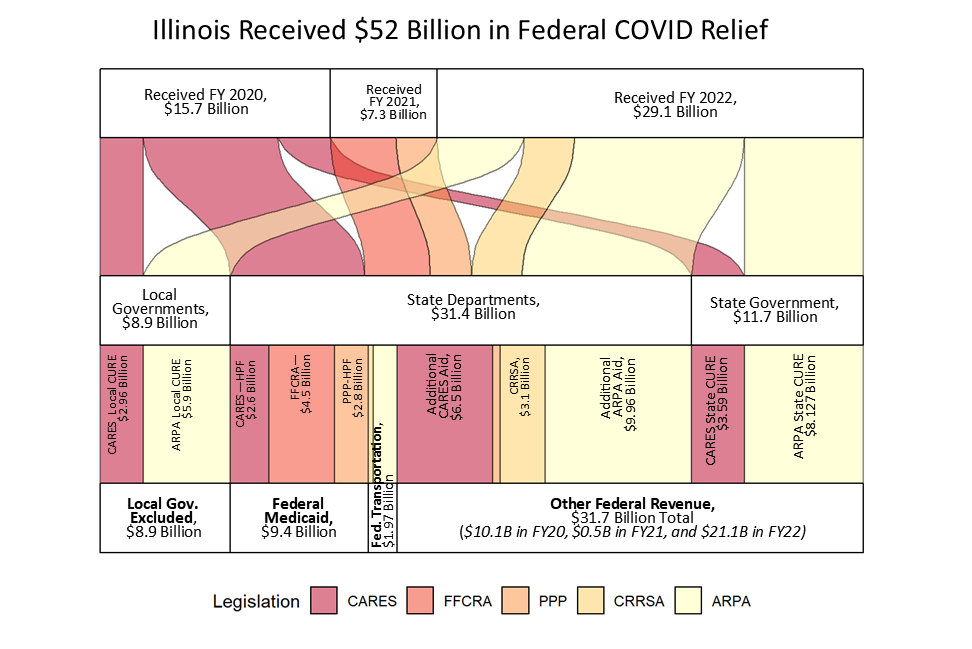
\includegraphics{./images/rev_CMT_52bil-01.png}

Local Governments within Illinois received \$8.9 billion for economic
recovery but we do not include funds given straight to localities in our
State COVID recovery fund calculations or Fiscal Gap analysis.

Additional labels were added using Publisher to create the image above.
Preliminary graphs and summed values for the image are calculated in the
code chunk below:

\begin{Shaded}
\begin{Highlighting}[]
\NormalTok{sankeydata }\OtherTok{\textless{}{-}} \FunctionTok{read\_excel}\NormalTok{(}\StringTok{"federalcoviddollars.xlsx"}\NormalTok{)}

\NormalTok{sankey }\OtherTok{\textless{}{-}}\NormalTok{ sankeydata }\SpecialCharTok{\%\textgreater{}\%} 
  \CommentTok{\#select(Federal, StateFunds, StFund, Expenditures, stfundname, value, Notes) \%\textgreater{}\%}
  \CommentTok{\#  filter(StFund == "Total") \%\textgreater{}\%}

  \FunctionTok{mutate}\NormalTok{(}\AttributeTok{StateFunds =} \FunctionTok{factor}\NormalTok{(FY, }\AttributeTok{levels =} \FunctionTok{c}\NormalTok{( }\StringTok{"FY20"}\NormalTok{, }\StringTok{"FY21"}\NormalTok{, }\StringTok{"FY22"}\NormalTok{)),}
        \AttributeTok{Legislation2 =} \FunctionTok{factor}\NormalTok{(Legislation2, }\AttributeTok{levels =} \FunctionTok{c}\NormalTok{( }\StringTok{"Other"}\NormalTok{, }\StringTok{"CARES"}\NormalTok{, }\StringTok{"CRRSA"}\NormalTok{, }\StringTok{"ARPA"}\NormalTok{)),}
                              \AttributeTok{Legislation =} \FunctionTok{factor}\NormalTok{(Legislation, }\AttributeTok{levels =} \FunctionTok{c}\NormalTok{( }\StringTok{"CARES"}\NormalTok{, }\StringTok{"FFCRA"}\NormalTok{,}\StringTok{"PPP"}\NormalTok{, }\StringTok{"CRRSA"}\NormalTok{, }\StringTok{"ARPA"}\NormalTok{))}
\NormalTok{)}
         
                 \CommentTok{\#  Expenditures = factor(Expenditures, levels = c("Community Development", "Public Health", "Medicaid", "K{-}12", "Federal Other", "Transit")),}
      \CommentTok{\#   Notes = factor(Notes, levels = c(  "CARES", "Other *","CRRSA", "ARPA")))}


\FunctionTok{ggplot}\NormalTok{(sankey, }
       \FunctionTok{aes}\NormalTok{(}\AttributeTok{y =} \StringTok{\textasciigrave{}}\AttributeTok{Dollars Received}\StringTok{\textasciigrave{}}\NormalTok{, }\AttributeTok{axis3 =}\NormalTok{ FY, }\AttributeTok{axis2 =} \StringTok{\textasciigrave{}}\AttributeTok{Broad Category}\StringTok{\textasciigrave{}}\NormalTok{, }\AttributeTok{axis1=}\NormalTok{FF\_Cat2, }\AttributeTok{label =} \StringTok{"stratum"}\NormalTok{)) }\SpecialCharTok{+}
  \FunctionTok{geom\_flow}\NormalTok{(}\FunctionTok{aes}\NormalTok{(}\AttributeTok{fill =}\NormalTok{ Legislation), }\AttributeTok{color =} \StringTok{"black"}\NormalTok{, }\AttributeTok{reverse=}\ConstantTok{FALSE}\NormalTok{) }\SpecialCharTok{+}
 \CommentTok{\# guides(fill = FALSE) +   }
  \FunctionTok{geom\_stratum}\NormalTok{(}\AttributeTok{reverse=}\ConstantTok{FALSE}\NormalTok{) }\SpecialCharTok{+}
\FunctionTok{coord\_flip}\NormalTok{() }\SpecialCharTok{+}
   \FunctionTok{scale\_fill\_brewer}\NormalTok{(}\AttributeTok{palette =} \StringTok{"YlOrRd"}\NormalTok{, }\AttributeTok{direction =} \SpecialCharTok{{-}}\DecValTok{1}\NormalTok{) }\SpecialCharTok{+}
  \FunctionTok{theme\_void}\NormalTok{() }\SpecialCharTok{+}
     \FunctionTok{geom\_text}\NormalTok{(}\AttributeTok{stat =} \StringTok{"stratum"}\NormalTok{, }\FunctionTok{aes}\NormalTok{(}\AttributeTok{label =} \FunctionTok{after\_stat}\NormalTok{(stratum)), }\AttributeTok{size =} \DecValTok{2}\NormalTok{, }\AttributeTok{reverse=}\ConstantTok{FALSE}\NormalTok{)}\SpecialCharTok{+}
    \FunctionTok{theme}\NormalTok{(}\AttributeTok{legend.position =} \StringTok{"bottom"}\NormalTok{) }\SpecialCharTok{+}
  \FunctionTok{labs}\NormalTok{(}\AttributeTok{title =} \StringTok{"$52 Billion in Federal Aid has been Committed to Illinois"}\NormalTok{, }\AttributeTok{subtitle =} \StringTok{"State Fiscal Years 2020{-}2022"}\NormalTok{)}
\end{Highlighting}
\end{Shaded}

\begin{figure}[H]

{\centering 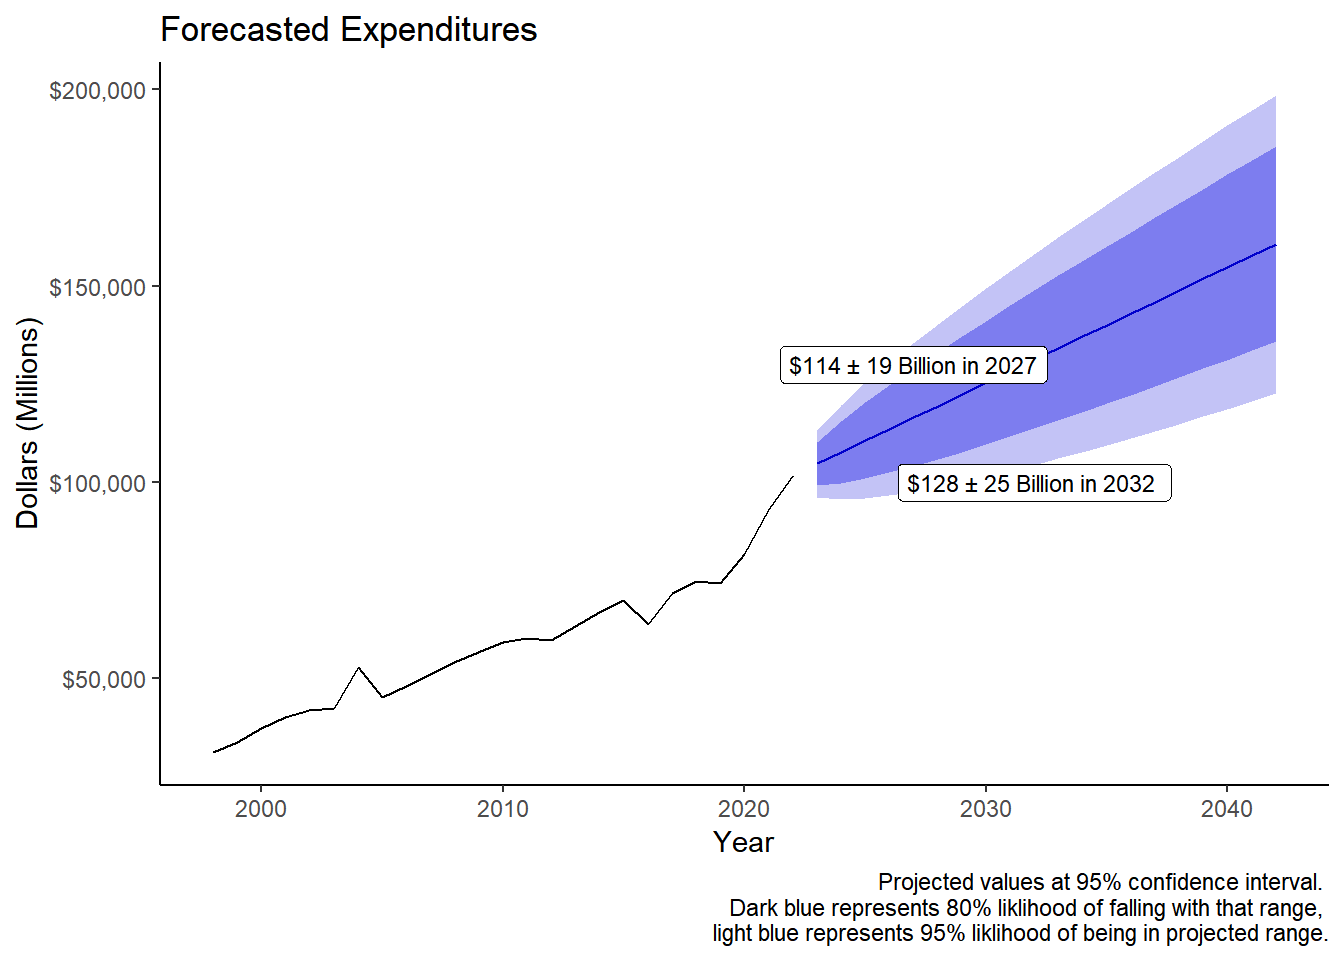
\includegraphics{./FedMoneyReceived_files/figure-pdf/unnamed-chunk-23-1.pdf}

}

\end{figure}

\begin{Shaded}
\begin{Highlighting}[]
\FunctionTok{ggplot}\NormalTok{(sankey, }
       \FunctionTok{aes}\NormalTok{(}\AttributeTok{y =} \StringTok{\textasciigrave{}}\AttributeTok{Dollars Received}\StringTok{\textasciigrave{}}\NormalTok{, }\AttributeTok{axis3 =}\NormalTok{ FY, }\AttributeTok{axis1 =} \StringTok{\textasciigrave{}}\AttributeTok{Broad Category}\StringTok{\textasciigrave{}}\NormalTok{, }\AttributeTok{axis2=}\NormalTok{FF\_Cat2, }\AttributeTok{label =} \StringTok{"stratum"}\NormalTok{)) }\SpecialCharTok{+}
  \FunctionTok{geom\_flow}\NormalTok{(}\FunctionTok{aes}\NormalTok{(}\AttributeTok{fill =}\NormalTok{ Legislation), }\AttributeTok{color =} \StringTok{"black"}\NormalTok{, }\AttributeTok{reverse=}\ConstantTok{FALSE}\NormalTok{) }\SpecialCharTok{+}
 \CommentTok{\# guides(fill = FALSE) +   }
  \FunctionTok{geom\_stratum}\NormalTok{(}\AttributeTok{reverse=}\ConstantTok{FALSE}\NormalTok{) }\SpecialCharTok{+}
\FunctionTok{coord\_flip}\NormalTok{() }\SpecialCharTok{+}
   \FunctionTok{scale\_fill\_brewer}\NormalTok{(}\AttributeTok{palette =} \StringTok{"YlOrRd"}\NormalTok{, }\AttributeTok{direction =} \SpecialCharTok{{-}}\DecValTok{1}\NormalTok{) }\SpecialCharTok{+}
  \FunctionTok{theme\_void}\NormalTok{() }\SpecialCharTok{+}
     \FunctionTok{geom\_text}\NormalTok{(}\AttributeTok{stat =} \StringTok{"stratum"}\NormalTok{, }\FunctionTok{aes}\NormalTok{(}\AttributeTok{label =} \FunctionTok{after\_stat}\NormalTok{(stratum)), }\AttributeTok{size =} \DecValTok{2}\NormalTok{, }\AttributeTok{reverse=}\ConstantTok{FALSE}\NormalTok{)}\SpecialCharTok{+}
    \FunctionTok{theme}\NormalTok{(}\AttributeTok{legend.position =} \StringTok{"bottom"}\NormalTok{) }\SpecialCharTok{+}
  \FunctionTok{labs}\NormalTok{(}\AttributeTok{title =} \StringTok{"$52 Billion in Federal Aid has been Committed to Illinois"}\NormalTok{, }\AttributeTok{subtitle =} \StringTok{"State Fiscal Years 2020{-}2022"}\NormalTok{)}
\end{Highlighting}
\end{Shaded}

\begin{figure}[H]

{\centering 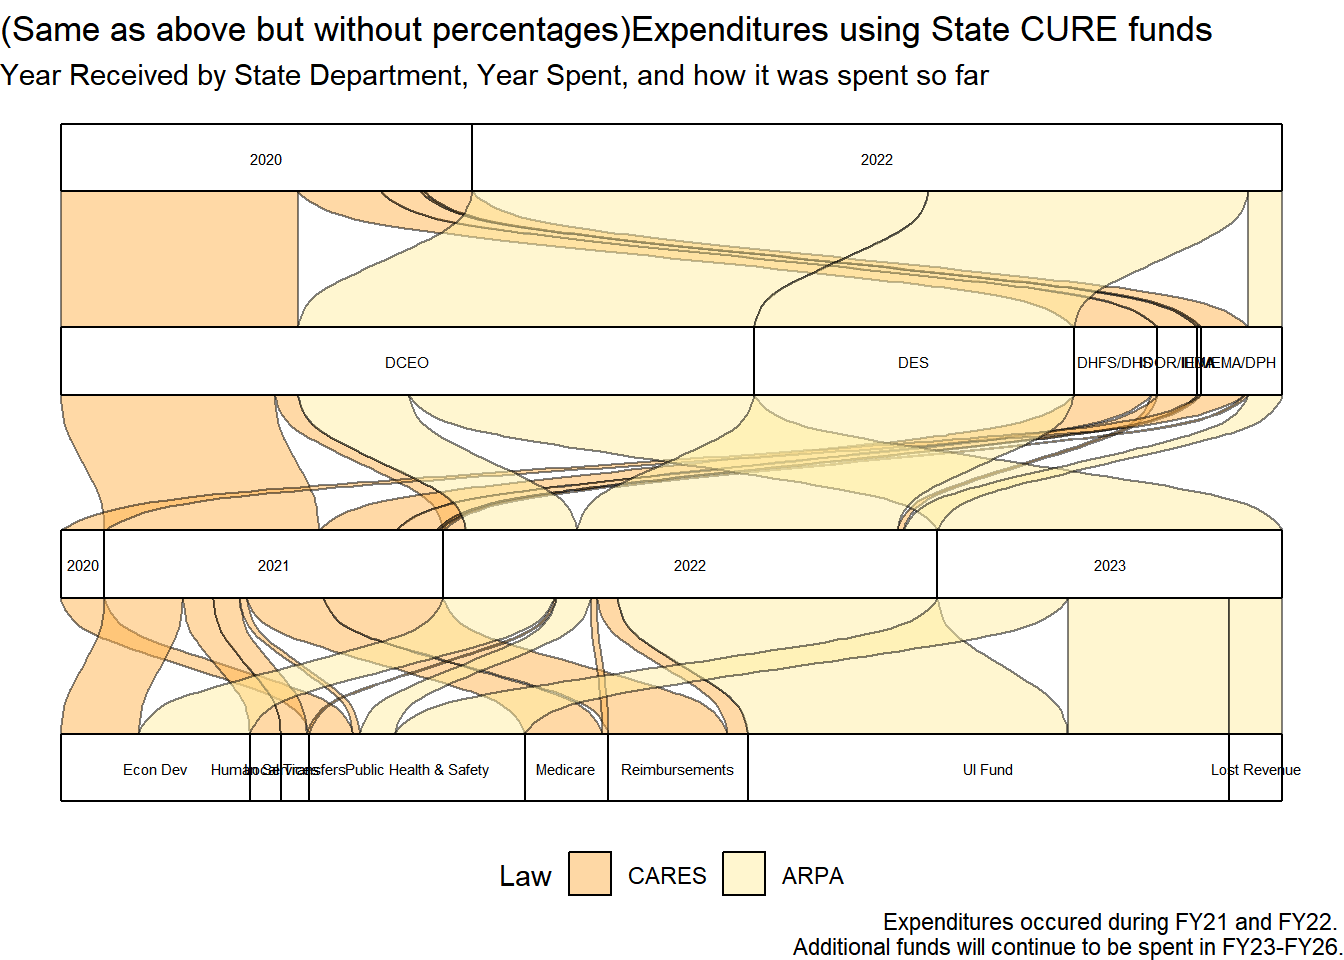
\includegraphics{./FedMoneyReceived_files/figure-pdf/unnamed-chunk-23-2.pdf}

}

\end{figure}

\begin{Shaded}
\begin{Highlighting}[]
\NormalTok{sankey }\SpecialCharTok{\%\textgreater{}\%} 
  \FunctionTok{group\_by}\NormalTok{(FY) }\SpecialCharTok{\%\textgreater{}\%} 
  \FunctionTok{summarize}\NormalTok{(}\AttributeTok{sum=}\FunctionTok{sum}\NormalTok{(}\StringTok{\textasciigrave{}}\AttributeTok{Dollars Received}\StringTok{\textasciigrave{}}\NormalTok{))}
\end{Highlighting}
\end{Shaded}

\begin{verbatim}
# A tibble: 3 x 2
  FY            sum
  <chr>       <dbl>
1 FY20  15705249790
2 FY21   7263242245
3 FY22  29056349119
\end{verbatim}

\begin{Shaded}
\begin{Highlighting}[]
\NormalTok{sankey }\SpecialCharTok{\%\textgreater{}\%} 
  \FunctionTok{group\_by}\NormalTok{(Legislation) }\SpecialCharTok{\%\textgreater{}\%} 
  \FunctionTok{summarize}\NormalTok{(}\AttributeTok{sum=}\FunctionTok{sum}\NormalTok{(}\StringTok{\textasciigrave{}}\AttributeTok{Dollars Received}\StringTok{\textasciigrave{}}\NormalTok{))}
\end{Highlighting}
\end{Shaded}

\begin{verbatim}
# A tibble: 5 x 2
  Legislation         sum
  <fct>             <dbl>
1 CARES       15705249790
2 FFCRA        4469242245
3 PPP          2794000000
4 CRRSA        3426118654
5 ARPA        25630230465
\end{verbatim}

\begin{Shaded}
\begin{Highlighting}[]
\NormalTok{sankey }\SpecialCharTok{\%\textgreater{}\%} 
  \FunctionTok{group\_by}\NormalTok{(}\StringTok{\textasciigrave{}}\AttributeTok{Broad Category}\StringTok{\textasciigrave{}}\NormalTok{) }\SpecialCharTok{\%\textgreater{}\%} 
  \FunctionTok{summarize}\NormalTok{(}\AttributeTok{sum=}\FunctionTok{sum}\NormalTok{(}\StringTok{\textasciigrave{}}\AttributeTok{Dollars Received}\StringTok{\textasciigrave{}}\NormalTok{))}
\end{Highlighting}
\end{Shaded}

\begin{verbatim}
# A tibble: 3 x 2
  `Broad Category`          sum
  <chr>                   <dbl>
1 Local Govs        10500618984
2 State Departments 29807277170
3 State Government  11716945000
\end{verbatim}

\begin{Shaded}
\begin{Highlighting}[]
\NormalTok{sankey }\SpecialCharTok{\%\textgreater{}\%} 
  \FunctionTok{group\_by}\NormalTok{(Legislation, FF\_Cat2) }\SpecialCharTok{\%\textgreater{}\%} 
  \FunctionTok{summarize}\NormalTok{(}\AttributeTok{sum=}\FunctionTok{sum}\NormalTok{(}\StringTok{\textasciigrave{}}\AttributeTok{Dollars Received}\StringTok{\textasciigrave{}}\NormalTok{))}
\end{Highlighting}
\end{Shaded}

\begin{verbatim}
# A tibble: 9 x 3
# Groups:   Legislation [5]
  Legislation FF_Cat2                       sum
  <fct>       <chr>                       <dbl>
1 CARES       Excluded               2955544419
2 CARES       Federal Medicare       2636263219
3 CARES       Other Federal Revenue 10113442152
4 FFCRA       Federal Medicare       4469242245
5 PPP         Federal Medicare       2290000000
6 PPP         Other Federal Revenue   504000000
7 CRRSA       Other Federal Revenue  3426118654
8 ARPA        Excluded               7545074565
9 ARPA        Other Federal Revenue 18085155900
\end{verbatim}

\begin{Shaded}
\begin{Highlighting}[]
\NormalTok{sankey }\SpecialCharTok{\%\textgreater{}\%} 
  \FunctionTok{group\_by}\NormalTok{(FF\_Cat2) }\SpecialCharTok{\%\textgreater{}\%} 
  \FunctionTok{summarize}\NormalTok{(}\AttributeTok{sum=}\FunctionTok{sum}\NormalTok{(}\StringTok{\textasciigrave{}}\AttributeTok{Dollars Received}\StringTok{\textasciigrave{}}\NormalTok{))}
\end{Highlighting}
\end{Shaded}

\begin{verbatim}
# A tibble: 3 x 2
  FF_Cat2                       sum
  <chr>                       <dbl>
1 Excluded              10500618984
2 Federal Medicare       9395505464
3 Other Federal Revenue 32128716706
\end{verbatim}

\begin{Shaded}
\begin{Highlighting}[]
\NormalTok{sankey }\SpecialCharTok{\%\textgreater{}\%} 
  \FunctionTok{group\_by}\NormalTok{(Legislation, }\StringTok{\textasciigrave{}}\AttributeTok{Broad Category}\StringTok{\textasciigrave{}}\NormalTok{,FF\_Cat2) }\SpecialCharTok{\%\textgreater{}\%} 
  \FunctionTok{summarize}\NormalTok{(}\AttributeTok{sum=}\FunctionTok{sum}\NormalTok{(}\StringTok{\textasciigrave{}}\AttributeTok{Dollars Received}\StringTok{\textasciigrave{}}\NormalTok{))}
\end{Highlighting}
\end{Shaded}

\begin{verbatim}
# A tibble: 11 x 4
# Groups:   Legislation, Broad Category [9]
   Legislation `Broad Category`  FF_Cat2                      sum
   <fct>       <chr>             <chr>                      <dbl>
 1 CARES       Local Govs        Excluded              2955544419
 2 CARES       State Departments Federal Medicare      2636263219
 3 CARES       State Departments Other Federal Revenue 6523497152
 4 CARES       State Government  Other Federal Revenue 3589945000
 5 FFCRA       State Departments Federal Medicare      4469242245
 6 PPP         State Departments Federal Medicare      2290000000
 7 PPP         State Departments Other Federal Revenue  504000000
 8 CRRSA       State Departments Other Federal Revenue 3426118654
 9 ARPA        Local Govs        Excluded              7545074565
10 ARPA        State Departments Other Federal Revenue 9958155900
11 ARPA        State Government  Other Federal Revenue 8127000000
\end{verbatim}

\begin{Shaded}
\begin{Highlighting}[]
\NormalTok{sankey }\SpecialCharTok{\%\textgreater{}\%} 
  \FunctionTok{group\_by}\NormalTok{(FY, FF\_Cat2) }\SpecialCharTok{\%\textgreater{}\%} 
  \FunctionTok{summarize}\NormalTok{(}\AttributeTok{sum=}\FunctionTok{sum}\NormalTok{(}\StringTok{\textasciigrave{}}\AttributeTok{Dollars Received}\StringTok{\textasciigrave{}}\NormalTok{)) }\SpecialCharTok{\%\textgreater{}\%} 
  \FunctionTok{pivot\_wider}\NormalTok{(}\AttributeTok{names\_from=}\StringTok{"FY"}\NormalTok{, }\AttributeTok{values\_from =}\NormalTok{ sum)}
\end{Highlighting}
\end{Shaded}

\begin{verbatim}
# A tibble: 3 x 4
  FF_Cat2                      FY20       FY21        FY22
  <chr>                       <dbl>      <dbl>       <dbl>
1 Excluded               2955544419         NA  7545074565
2 Federal Medicare       2636263219 6759242245          NA
3 Other Federal Revenue 10113442152  504000000 21511274554
\end{verbatim}

Illinois received \$11.6 billion dollars from State Fiscal Recovery
Funds into its State CURE fund and also received \$31.4 billion in other
federal revenue to Illinois State departments. This other federal
revenue frequently came in the form of increased or new grants to many
State Departments that normally receive federal funding.

\hypertarget{committed-totals---excluding-local-government-funds}{%
\subsection{Committed Totals - Excluding Local Government
Funds}\label{committed-totals---excluding-local-government-funds}}

Below is a graph showing federal stimulus money that was committed in
each year, the federal agency/fund that it came from, and what kind of
revenue it was considered (Federal Other, transportation, or medicaid)
who received the money (e.g.~the State of Illinois, Department of Human
Services, Local Governments, etc.). Again, these graphs show the funds
that were committed to Illinois and their intended purpose, NOT the data
on how or when it was spent.

When Local Funds are included, \$15.7 billion was received in FY20,
\$7.24 billion in FY21, and \$29 billion was received in FY22 from
multiple COVID response Federal Acts.

Around \$43 billion went to the state and \$8.8 billion went to straight
to local governments. When excluding the money that went straight to
local governments, the state received \$12.7 billion in FY20 (CARES
Act), \$7.24 billion in FY21, and \$23 billion was committed in FY22
(ARP Act). This includes both State CURE funds that had more flexibility
in how they were spent as well as the grants and that went to State
Departments for specific purposes.

The code below creates same graph as above but funds that went straight
to Local Governments (cities and counties) are dropped from the totals.

\begin{Shaded}
\begin{Highlighting}[]
\NormalTok{sankey }\SpecialCharTok{\%\textgreater{}\%} 
  \FunctionTok{filter}\NormalTok{(FF\_Cat2}\SpecialCharTok{!=} \StringTok{"Excluded"}\NormalTok{) }\SpecialCharTok{\%\textgreater{}\%}

  \FunctionTok{ggplot}\NormalTok{(}\FunctionTok{aes}\NormalTok{(}\AttributeTok{y =} \StringTok{\textasciigrave{}}\AttributeTok{Dollars Received}\StringTok{\textasciigrave{}}\NormalTok{, }\AttributeTok{axis3 =}\NormalTok{ FY, }\AttributeTok{axis2 =} \StringTok{\textasciigrave{}}\AttributeTok{Broad Category}\StringTok{\textasciigrave{}}\NormalTok{, }\AttributeTok{axis1=}\NormalTok{FF\_Cat2, }\AttributeTok{label =} \StringTok{"stratum"}\NormalTok{)) }\SpecialCharTok{+}
  \FunctionTok{geom\_flow}\NormalTok{(}\FunctionTok{aes}\NormalTok{(}\AttributeTok{fill =}\NormalTok{ Legislation), }\AttributeTok{color =} \StringTok{"black"}\NormalTok{, }\AttributeTok{reverse=}\ConstantTok{FALSE}\NormalTok{) }\SpecialCharTok{+}
 \CommentTok{\# guides(fill = FALSE) +   }
  \FunctionTok{geom\_stratum}\NormalTok{(}\AttributeTok{reverse=}\ConstantTok{FALSE}\NormalTok{)}\SpecialCharTok{+}
\FunctionTok{coord\_flip}\NormalTok{()}\SpecialCharTok{+}
   \FunctionTok{scale\_fill\_brewer}\NormalTok{(}\AttributeTok{palette =} \StringTok{"YlOrRd"}\NormalTok{, }\AttributeTok{direction =} \SpecialCharTok{{-}}\DecValTok{1}\NormalTok{)}\SpecialCharTok{+}
  \FunctionTok{theme\_void}\NormalTok{() }\SpecialCharTok{+}
     \FunctionTok{geom\_text}\NormalTok{(}\AttributeTok{stat =} \StringTok{"stratum"}\NormalTok{, }\FunctionTok{aes}\NormalTok{(}\AttributeTok{label =} \FunctionTok{after\_stat}\NormalTok{(stratum)), }\AttributeTok{size =} \DecValTok{2}\NormalTok{, }\AttributeTok{reverse=}\ConstantTok{FALSE}\NormalTok{)}\SpecialCharTok{+}
    \FunctionTok{theme}\NormalTok{(}\AttributeTok{legend.position =} \StringTok{"bottom"}\NormalTok{)}\SpecialCharTok{+}
  \FunctionTok{ggtitle}\NormalTok{(}\StringTok{"Without Local government relief:}
\StringTok{          $12.7 Billion in FY20, $7 Billion in FY21, and $23 Billion in FY22 Committed to Illinois"}\NormalTok{)}
\end{Highlighting}
\end{Shaded}

\begin{figure}[H]

{\centering 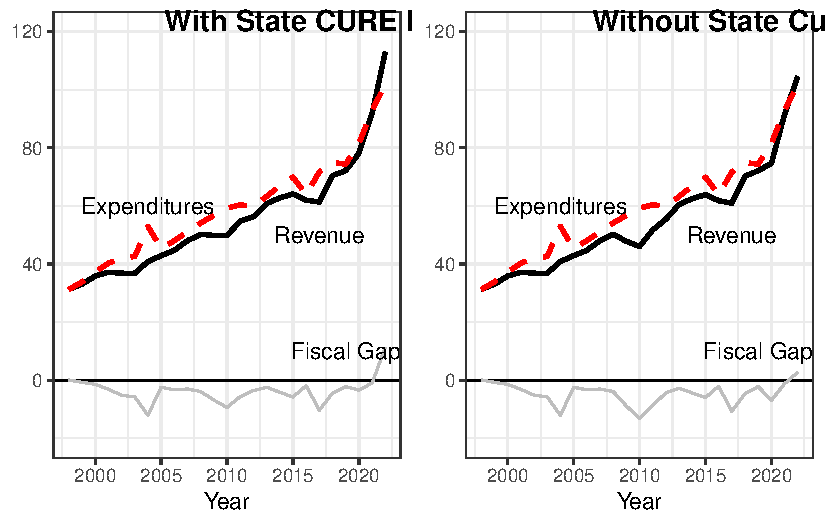
\includegraphics{./FedMoneyReceived_files/figure-pdf/unnamed-chunk-26-1.pdf}

}

\end{figure}

\begin{Shaded}
\begin{Highlighting}[]
\NormalTok{sankey }\SpecialCharTok{\%\textgreater{}\%} \FunctionTok{filter}\NormalTok{(FF\_Cat2}\SpecialCharTok{!=} \StringTok{"Excluded"}\NormalTok{) }\SpecialCharTok{\%\textgreater{}\%}
  \FunctionTok{ggplot}\NormalTok{(}\FunctionTok{aes}\NormalTok{(}\AttributeTok{y =} \StringTok{\textasciigrave{}}\AttributeTok{Dollars Received}\StringTok{\textasciigrave{}}\NormalTok{, }\AttributeTok{axis4 =}\NormalTok{ FY, }\AttributeTok{axis3=} \StringTok{\textasciigrave{}}\AttributeTok{Category}\StringTok{\textasciigrave{}}\NormalTok{,  }\AttributeTok{axis1=}\NormalTok{FF\_Cat2}
          \CommentTok{\# , label = "stratum"}
\NormalTok{           )) }\SpecialCharTok{+}
  \FunctionTok{geom\_flow}\NormalTok{(}\FunctionTok{aes}\NormalTok{(}\AttributeTok{fill =}\NormalTok{ Legislation, }\AttributeTok{label =} \StringTok{"flow"}\NormalTok{), }
            \AttributeTok{color =} \StringTok{"black"}\NormalTok{, }\AttributeTok{reverse=}\ConstantTok{FALSE}\NormalTok{) }\SpecialCharTok{+}
 \CommentTok{\# guides(fill = FALSE) +   }
  \FunctionTok{geom\_stratum}\NormalTok{(}\AttributeTok{reverse=}\ConstantTok{FALSE}\NormalTok{)}\SpecialCharTok{+}
     \FunctionTok{geom\_text}\NormalTok{(}\AttributeTok{stat =} \StringTok{"stratum"}\NormalTok{, }\FunctionTok{aes}\NormalTok{(}\AttributeTok{label =} \FunctionTok{after\_stat}\NormalTok{(stratum)), }
               \AttributeTok{size =} \DecValTok{3}\NormalTok{, }\AttributeTok{reverse=}\ConstantTok{FALSE}\NormalTok{)}\SpecialCharTok{+}
  \FunctionTok{coord\_flip}\NormalTok{()}\SpecialCharTok{+}
  \FunctionTok{scale\_fill\_brewer}\NormalTok{(}\AttributeTok{palette =} \StringTok{"YlOrRd"}\NormalTok{, }\AttributeTok{direction =} \SpecialCharTok{{-}}\DecValTok{1}\NormalTok{)}\SpecialCharTok{+}
  \FunctionTok{theme\_void}\NormalTok{() }\SpecialCharTok{+}
  \FunctionTok{theme}\NormalTok{(}\AttributeTok{legend.position =} \StringTok{"bottom"}\NormalTok{, }\AttributeTok{legend.title=}\FunctionTok{element\_blank}\NormalTok{())}\SpecialCharTok{+}
  \FunctionTok{ggtitle}\NormalTok{(}\StringTok{"Without Local government relief:}
\StringTok{          $12.7 Billion in FY20, $7.3 Billion in FY21, and $21.5 Billion in FY22 Committed to Illinois"}\NormalTok{)}
\end{Highlighting}
\end{Shaded}

\begin{figure}[H]

{\centering \includegraphics{./FedMoneyReceived_files/figure-pdf/unnamed-chunk-26-2.pdf}

}

\end{figure}

\begin{Shaded}
\begin{Highlighting}[]
\CommentTok{\# without local government CURE funds}
\NormalTok{sankey }\SpecialCharTok{\%\textgreater{}\%} 
  \FunctionTok{filter}\NormalTok{(FF\_Cat2 }\SpecialCharTok{!=} \StringTok{"Excluded"}\NormalTok{) }\SpecialCharTok{\%\textgreater{}\%} 
  \FunctionTok{group\_by}\NormalTok{(FY)}\SpecialCharTok{\%\textgreater{}\%}
  \FunctionTok{summarize}\NormalTok{(}\AttributeTok{TotalReceived=}\FunctionTok{sum}\NormalTok{(}\StringTok{\textasciigrave{}}\AttributeTok{Dollars Received}\StringTok{\textasciigrave{}}\NormalTok{))}
\end{Highlighting}
\end{Shaded}

\begin{verbatim}
# A tibble: 3 x 2
  FY    TotalReceived
  <chr>         <dbl>
1 FY20    12749705371
2 FY21     7263242245
3 FY22    21511274554
\end{verbatim}

\begin{Shaded}
\begin{Highlighting}[]
\NormalTok{sankey }\SpecialCharTok{\%\textgreater{}\%} \FunctionTok{group\_by}\NormalTok{(FY)}\SpecialCharTok{\%\textgreater{}\%}\FunctionTok{summarize}\NormalTok{(}\AttributeTok{TotalReceived=}\FunctionTok{sum}\NormalTok{(}\StringTok{\textasciigrave{}}\AttributeTok{Dollars Received}\StringTok{\textasciigrave{}}\NormalTok{))}
\end{Highlighting}
\end{Shaded}

\begin{verbatim}
# A tibble: 3 x 2
  FY    TotalReceived
  <chr>         <dbl>
1 FY20    15705249790
2 FY21     7263242245
3 FY22    29056349119
\end{verbatim}

\begin{Shaded}
\begin{Highlighting}[]
\NormalTok{sankey }\SpecialCharTok{\%\textgreater{}\%} \FunctionTok{group\_by}\NormalTok{(Legislation)}\SpecialCharTok{\%\textgreater{}\%}\FunctionTok{summarize}\NormalTok{(}\AttributeTok{TotalReceived=}\FunctionTok{sum}\NormalTok{(}\StringTok{\textasciigrave{}}\AttributeTok{Dollars Received}\StringTok{\textasciigrave{}}\NormalTok{))}
\end{Highlighting}
\end{Shaded}

\begin{verbatim}
# A tibble: 5 x 2
  Legislation TotalReceived
  <fct>               <dbl>
1 CARES         15705249790
2 FFCRA          4469242245
3 PPP            2794000000
4 CRRSA          3426118654
5 ARPA          25630230465
\end{verbatim}

\begin{Shaded}
\begin{Highlighting}[]
\NormalTok{sankey }\SpecialCharTok{\%\textgreater{}\%} \FunctionTok{group\_by}\NormalTok{(Recipient)}\SpecialCharTok{\%\textgreater{}\%}\FunctionTok{summarize}\NormalTok{(}\AttributeTok{TotalReceived=}\FunctionTok{sum}\NormalTok{(}\StringTok{\textasciigrave{}}\AttributeTok{Dollars Received}\StringTok{\textasciigrave{}}\NormalTok{))}
\end{Highlighting}
\end{Shaded}

\begin{verbatim}
# A tibble: 5 x 2
  Recipient           TotalReceived
  <chr>                       <dbl>
1 Human Services         3627363000
2 ISBE                   8031662158
3 Local Govs-Excluded   10500618984
4 Other                  5827917414
5 State                 24037279598
\end{verbatim}

\begin{Shaded}
\begin{Highlighting}[]
\NormalTok{sankey }\SpecialCharTok{\%\textgreater{}\%} \FunctionTok{group\_by}\NormalTok{(FF\_Cat)}\SpecialCharTok{\%\textgreater{}\%}\FunctionTok{summarize}\NormalTok{(}\AttributeTok{TotalReceived=}\FunctionTok{sum}\NormalTok{(}\StringTok{\textasciigrave{}}\AttributeTok{Dollars Received}\StringTok{\textasciigrave{}}\NormalTok{))}
\end{Highlighting}
\end{Shaded}

\begin{verbatim}
# A tibble: 7 x 2
  FF_Cat        TotalReceived
  <chr>                 <dbl>
1 Excluded        10500618984
2 Federal Other    7110635965
3 K-12             8031662158
4 Medicare         9395505464
5 Other            4984990736
6 State CURE      11645945000
7 Transit           355482847
\end{verbatim}

\begin{Shaded}
\begin{Highlighting}[]
\NormalTok{sankey }\SpecialCharTok{\%\textgreater{}\%} \FunctionTok{group\_by}\NormalTok{(Legislation, Recipient)}\SpecialCharTok{\%\textgreater{}\%}\FunctionTok{summarize}\NormalTok{(}\AttributeTok{TotalReceived=}\FunctionTok{sum}\NormalTok{(}\StringTok{\textasciigrave{}}\AttributeTok{Dollars Received}\StringTok{\textasciigrave{}}\NormalTok{)) }\SpecialCharTok{\%\textgreater{}\%} \FunctionTok{pivot\_wider}\NormalTok{(}\AttributeTok{names\_from =}\NormalTok{ Legislation, }\AttributeTok{values\_from =}\NormalTok{ TotalReceived)}
\end{Highlighting}
\end{Shaded}

\begin{verbatim}
# A tibble: 5 x 6
  Recipient                CARES      FFCRA        PPP      CRRSA       ARPA
  <chr>                    <dbl>      <dbl>      <dbl>      <dbl>      <dbl>
1 Human Services       165000000         NA         NA         NA 3462363000
2 ISBE                 677964975         NA         NA 2298709129 5054988054
3 Local Govs-Excluded 2955544419         NA         NA         NA 7545074565
4 Other               5055990736         NA         NA  771926678         NA
5 State               6850749660 4469242245 2794000000  355482847 9567804846
\end{verbatim}

\begin{Shaded}
\begin{Highlighting}[]
\NormalTok{sankey }\SpecialCharTok{\%\textgreater{}\%} \FunctionTok{group\_by}\NormalTok{(Legislation, FF\_Cat)}\SpecialCharTok{\%\textgreater{}\%}\FunctionTok{summarize}\NormalTok{(}\AttributeTok{TotalReceived=}\FunctionTok{sum}\NormalTok{(}\StringTok{\textasciigrave{}}\AttributeTok{Dollars Received}\StringTok{\textasciigrave{}}\NormalTok{)) }\SpecialCharTok{\%\textgreater{}\%} \FunctionTok{pivot\_wider}\NormalTok{(}\AttributeTok{names\_from =}\NormalTok{ Legislation, }\AttributeTok{values\_from =}\NormalTok{ TotalReceived)}
\end{Highlighting}
\end{Shaded}

\begin{verbatim}
# A tibble: 7 x 6
  FF_Cat             CARES      FFCRA        PPP      CRRSA       ARPA
  <chr>              <dbl>      <dbl>      <dbl>      <dbl>      <dbl>
1 Excluded      2955544419         NA         NA         NA 7545074565
2 Federal Other  931541441         NA  504000000  771926678 4903167846
3 K-12           677964975         NA         NA 2298709129 5054988054
4 Medicare      2636263219 4469242245 2290000000         NA         NA
5 Other         4984990736         NA         NA         NA         NA
6 State CURE    3518945000         NA         NA         NA 8127000000
7 Transit               NA         NA         NA  355482847         NA
\end{verbatim}

\begin{Shaded}
\begin{Highlighting}[]
\NormalTok{sankey }\SpecialCharTok{\%\textgreater{}\%} \FunctionTok{group\_by}\NormalTok{(FY, FF\_Cat)}\SpecialCharTok{\%\textgreater{}\%}\FunctionTok{summarize}\NormalTok{(}\AttributeTok{TotalReceived=}\FunctionTok{sum}\NormalTok{(}\StringTok{\textasciigrave{}}\AttributeTok{Dollars Received}\StringTok{\textasciigrave{}}\NormalTok{)) }\SpecialCharTok{\%\textgreater{}\%} \FunctionTok{pivot\_wider}\NormalTok{(}\AttributeTok{names\_from =}\NormalTok{ FY, }\AttributeTok{values\_from =}\NormalTok{ TotalReceived)}
\end{Highlighting}
\end{Shaded}

\begin{verbatim}
# A tibble: 7 x 4
  FF_Cat              FY20       FY21       FY22
  <chr>              <dbl>      <dbl>      <dbl>
1 Excluded      2955544419         NA 7545074565
2 Federal Other  931541441  504000000 5675094524
3 K-12           677964975         NA 7353697183
4 Medicare      2636263219 6759242245         NA
5 Other         4984990736         NA         NA
6 State CURE    3518945000         NA 8127000000
7 Transit               NA         NA  355482847
\end{verbatim}

\begin{Shaded}
\begin{Highlighting}[]
\NormalTok{sankey }\SpecialCharTok{\%\textgreater{}\%} \FunctionTok{group\_by}\NormalTok{(Legislation, FF\_Cat2)}\SpecialCharTok{\%\textgreater{}\%}\FunctionTok{summarize}\NormalTok{(}\AttributeTok{TotalReceived=}\FunctionTok{sum}\NormalTok{(}\StringTok{\textasciigrave{}}\AttributeTok{Dollars Received}\StringTok{\textasciigrave{}}\NormalTok{)) }\SpecialCharTok{\%\textgreater{}\%} \FunctionTok{pivot\_wider}\NormalTok{(}\AttributeTok{names\_from =}\NormalTok{ Legislation, }\AttributeTok{values\_from =}\NormalTok{ TotalReceived)}
\end{Highlighting}
\end{Shaded}

\begin{verbatim}
# A tibble: 3 x 6
  FF_Cat2                     CARES      FFCRA        PPP      CRRSA        ARPA
  <chr>                       <dbl>      <dbl>      <dbl>      <dbl>       <dbl>
1 Excluded               2955544419         NA         NA         NA  7545074565
2 Federal Medicare       2636263219 4469242245 2290000000         NA          NA
3 Other Federal Revenue 10113442152         NA  504000000 3426118654 18085155900
\end{verbatim}

\begin{Shaded}
\begin{Highlighting}[]
\NormalTok{sankey }\SpecialCharTok{\%\textgreater{}\%} \FunctionTok{group\_by}\NormalTok{(FY, FF\_Cat2)}\SpecialCharTok{\%\textgreater{}\%}\FunctionTok{summarize}\NormalTok{(}\AttributeTok{TotalReceived=}\FunctionTok{sum}\NormalTok{(}\StringTok{\textasciigrave{}}\AttributeTok{Dollars Received}\StringTok{\textasciigrave{}}\NormalTok{)) }\SpecialCharTok{\%\textgreater{}\%} \FunctionTok{pivot\_wider}\NormalTok{(}\AttributeTok{names\_from =}\NormalTok{ FY, }\AttributeTok{values\_from =}\NormalTok{ TotalReceived)}
\end{Highlighting}
\end{Shaded}

\begin{verbatim}
# A tibble: 3 x 4
  FF_Cat2                      FY20       FY21        FY22
  <chr>                       <dbl>      <dbl>       <dbl>
1 Excluded               2955544419         NA  7545074565
2 Federal Medicare       2636263219 6759242245          NA
3 Other Federal Revenue 10113442152  504000000 21511274554
\end{verbatim}

\hypertarget{notes-on-sankey-graphs}{%
\subsubsection{Notes on Sankey Graphs}\label{notes-on-sankey-graphs}}

\href{https://cheatography.com/seleven/cheat-sheets/ggalluvial/}{ggsankey
info and example}

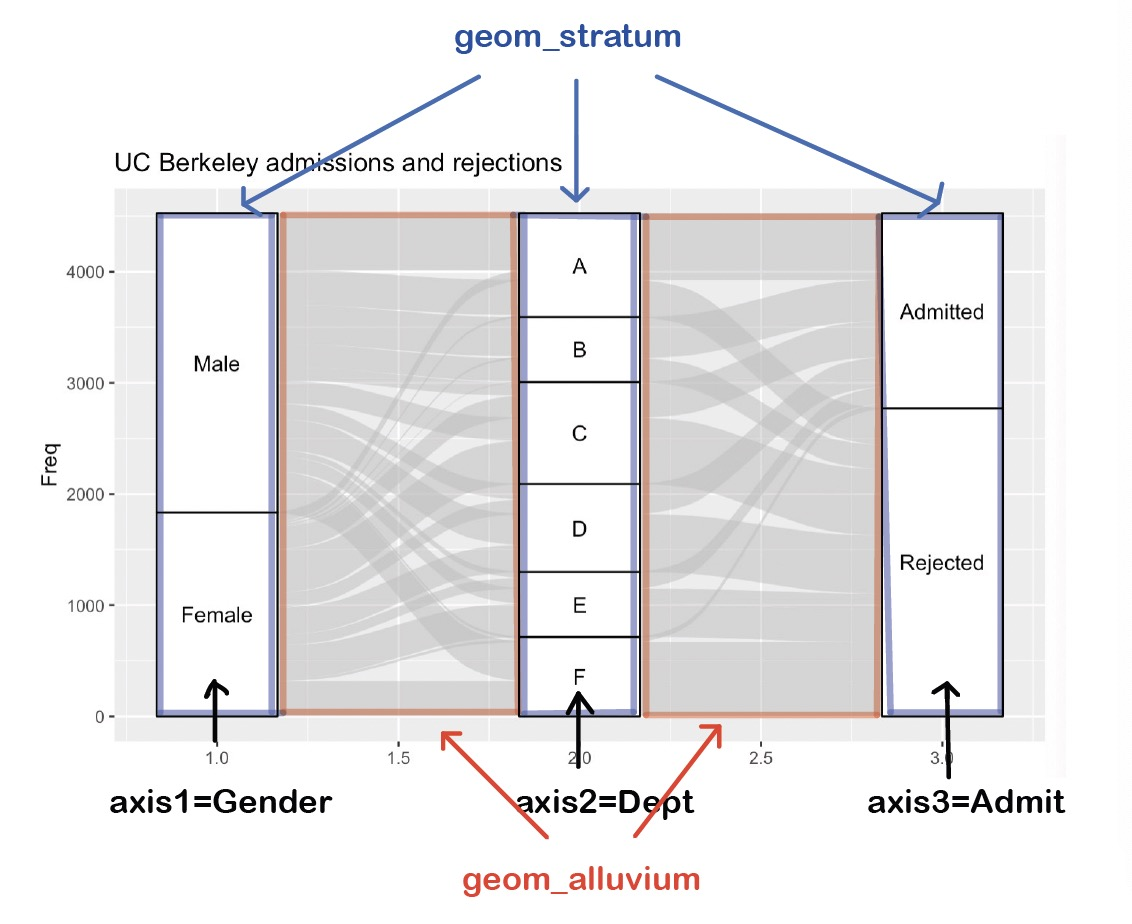
\includegraphics[width=3.60417in,height=\textheight]{./images/image-2109120559.png}

A little information on Sankey graphs is below:

\begin{itemize}
\tightlist
\item
  The axis is how the observations are grouped at each step. There are
  multiple axes.
\item
  Strata are the options that exist for each level. (e.g.~Year received
  can be 2021 or 2022)
\item
  Alluvium correspond to the fixed value of each axis variable.
  Proportional to how the sum of however you are grouping your data.
\item
  Flows are the segments of the alluvia between adjacent axes.
\end{itemize}

\bookmarksetup{startatroot}

\hypertarget{local-transfers}{%
\chapter{Local Transfers}\label{local-transfers}}

Separate transfers to local from parent agencies that come from DOR(492)
or Transportation (494). Treats muni revenue transfers as expenditures,
not negative revenue.

The share of certain taxes levied state-wide at a common rate and then
transferred to local governments. (Purely local-option taxes levied by
specific local governments with the state acting as collection agent are
NOT included.)

The six corresponding revenue items are:

\begin{itemize}
\tightlist
\item
  Local share of Personal Income Tax

  \begin{itemize}
  \tightlist
  \item
    Individual Income Tax Pass-Through New 2021 (source 2582).
  \end{itemize}
\item
  Local share of General Sales Tax
\item
  Personal Property Replacement Tax on Business Income
\item
  Personal Property Replacement Tax on Public Utilities
\item
  Local share of Motor Fuel Tax
\item
  Transportation Renewal Fund 0952
\end{itemize}

Until Dec 18. 2022, Local CURE was being aggregated into Revenue totals
since the agency was the Department of Revenue. However the \$371
million expenditure is for ``LOC GOVT ARPA'' and the revenue source that
is Local CURE is also \$371 million. Since it cancels out and is just
passed through the state government, I am changing changing the
fund\_ab\_in file so that in\_ff=0 for the Local CURE fund. It also
inflates the department of revenue expenditures in a misleading way when
the expense is actually a transfer to local governments.

\begin{itemize}
\item
  Dropping Local CURE fund from analysis results in a \$371 million
  decrease in the department of Revenue (where the Local Government ARPA
  transfer money). The appropriation for it was over \$740 million so
  some will probably be rolled over to FY23 too.
\item
  In the FY21 New and Reused Funds word document, 0325 Local CURE is
  described as \emph{``Created as a federal trust fund. The fund is
  established to receive transfers from either the disaster response and
  recovery fund or the state cure fund of federal funds received by the
  state. These transfers, subject to appropriation, will provide for the
  administration and payment of grants and expense reimbursements to
  units of local government. Revenues should be under Federal Other and
  expenditures under Commerce and Economic Opportunity.''} - Changed to
  Exclude.
\end{itemize}

\begin{Shaded}
\begin{Highlighting}[]
\FunctionTok{library}\NormalTok{(tidyverse)}
\FunctionTok{library}\NormalTok{(haven)}
\FunctionTok{library}\NormalTok{(formatR)}
\FunctionTok{library}\NormalTok{(lubridate)}
\FunctionTok{library}\NormalTok{(smooth)}
\FunctionTok{library}\NormalTok{(forecast)}
\FunctionTok{library}\NormalTok{(scales)}
\FunctionTok{library}\NormalTok{(kableExtra)}
\FunctionTok{library}\NormalTok{(ggplot2)}
\FunctionTok{library}\NormalTok{(readxl)}
\FunctionTok{library}\NormalTok{(tidyverse)}
\FunctionTok{library}\NormalTok{(data.table)}
\FunctionTok{library}\NormalTok{(quantmod)}
\FunctionTok{library}\NormalTok{(geofacet)}
\FunctionTok{library}\NormalTok{(janitor)}


\NormalTok{knitr}\SpecialCharTok{::}\NormalTok{opts\_chunk}\SpecialCharTok{$}\FunctionTok{set}\NormalTok{(}\AttributeTok{warning =} \ConstantTok{FALSE}\NormalTok{, }\AttributeTok{message =} \ConstantTok{FALSE}\NormalTok{)}

\NormalTok{exp\_temp }\OtherTok{\textless{}{-}} \FunctionTok{read\_csv}\NormalTok{(}\StringTok{"exp\_temp.csv"}\NormalTok{)}
\NormalTok{rev\_temp }\OtherTok{\textless{}{-}} \FunctionTok{read\_csv}\NormalTok{(}\StringTok{"rev\_temp.csv"}\NormalTok{)}
\end{Highlighting}
\end{Shaded}

\begin{Shaded}
\begin{Highlighting}[]
\NormalTok{exp\_temp }\OtherTok{\textless{}{-}}\NormalTok{ exp\_temp }\SpecialCharTok{\%\textgreater{}\%} 
  \FunctionTok{mutate}\NormalTok{(}
    \AttributeTok{agency =} \FunctionTok{case\_when}\NormalTok{(}
\NormalTok{      fund}\SpecialCharTok{==}\StringTok{"0515"} \SpecialCharTok{\&}\NormalTok{ object}\SpecialCharTok{==}\StringTok{"4470"} \SpecialCharTok{\&}\NormalTok{ type}\SpecialCharTok{==}\StringTok{"08"} \SpecialCharTok{\textasciitilde{}} \StringTok{"971"}\NormalTok{, }\CommentTok{\# income tax to local governments}
      
\NormalTok{      fund}\SpecialCharTok{==}\StringTok{"0515"} \SpecialCharTok{\&}\NormalTok{ object}\SpecialCharTok{==}\StringTok{"4491"} \SpecialCharTok{\&}\NormalTok{ type}\SpecialCharTok{==}\StringTok{"08"} \SpecialCharTok{\&}\NormalTok{ sequence}\SpecialCharTok{==}\StringTok{"00"} \SpecialCharTok{\textasciitilde{}} \StringTok{"971"}\NormalTok{, }\CommentTok{\# object is shared revenue payments}
      
\NormalTok{      fund}\SpecialCharTok{==}\StringTok{"0802"} \SpecialCharTok{\&}\NormalTok{ object}\SpecialCharTok{==}\StringTok{"4491"} \SpecialCharTok{\textasciitilde{}} \StringTok{"972"}\NormalTok{, }\CommentTok{\#pprt transfer}
      
\NormalTok{      fund}\SpecialCharTok{==}\StringTok{"0515"} \SpecialCharTok{\&}\NormalTok{ object}\SpecialCharTok{==}\StringTok{"4491"} \SpecialCharTok{\&}\NormalTok{ type}\SpecialCharTok{==}\StringTok{"08"} \SpecialCharTok{\&}\NormalTok{ sequence}\SpecialCharTok{==}\StringTok{"01"} \SpecialCharTok{\textasciitilde{}} \StringTok{"976"}\NormalTok{, }\CommentTok{\#gst to local}
      
\NormalTok{      fund}\SpecialCharTok{==}\StringTok{"0627"} \SpecialCharTok{\&}\NormalTok{ object}\SpecialCharTok{==}\StringTok{"4472"}\SpecialCharTok{\textasciitilde{}} \StringTok{"976"}\NormalTok{ , }\CommentTok{\# public transportation fund but no observations exist}
      
\NormalTok{      fund}\SpecialCharTok{==}\StringTok{"0648"} \SpecialCharTok{\&}\NormalTok{ object}\SpecialCharTok{==}\StringTok{"4472"} \SpecialCharTok{\textasciitilde{}} \StringTok{"976"}\NormalTok{, }\CommentTok{\# downstate public transportation, but doesn\textquotesingle{}t exist}
      
\NormalTok{      fund}\SpecialCharTok{==}\StringTok{"0515"} \SpecialCharTok{\&}\NormalTok{ object}\SpecialCharTok{==}\StringTok{"4470"} \SpecialCharTok{\&}\NormalTok{ type}\SpecialCharTok{==}\StringTok{"00"} \SpecialCharTok{\textasciitilde{}} \StringTok{"976"}\NormalTok{, }\CommentTok{\# object 4470 is grants to local governments}
      
\NormalTok{      object}\SpecialCharTok{==}\StringTok{"4491"} \SpecialCharTok{\&}\NormalTok{ (fund}\SpecialCharTok{==}\StringTok{"0188"}\SpecialCharTok{|}\NormalTok{fund}\SpecialCharTok{==}\StringTok{"0189"}\NormalTok{) }\SpecialCharTok{\textasciitilde{}} \StringTok{"976"}\NormalTok{,}
      
\NormalTok{      fund}\SpecialCharTok{==}\StringTok{"0187"} \SpecialCharTok{\&}\NormalTok{ object}\SpecialCharTok{==}\StringTok{"4470"} \SpecialCharTok{\textasciitilde{}} \StringTok{"976"}\NormalTok{,}
      
\NormalTok{      fund}\SpecialCharTok{==}\StringTok{"0186"} \SpecialCharTok{\&}\NormalTok{ object}\SpecialCharTok{==}\StringTok{"4470"} \SpecialCharTok{\textasciitilde{}} \StringTok{"976"}\NormalTok{,}
      
\NormalTok{      object}\SpecialCharTok{==}\StringTok{"4491"} \SpecialCharTok{\&}\NormalTok{ (fund}\SpecialCharTok{==}\StringTok{"0413"}\SpecialCharTok{|}\NormalTok{fund}\SpecialCharTok{==}\StringTok{"0414"}\SpecialCharTok{|}\NormalTok{fund}\SpecialCharTok{==}\StringTok{"0415"}\NormalTok{)  }\SpecialCharTok{\textasciitilde{}} \StringTok{"975"}\NormalTok{, }\CommentTok{\#mft to local}
\NormalTok{      fund }\SpecialCharTok{==} \StringTok{"0952"}\SpecialCharTok{\textasciitilde{}} \StringTok{"975"}\NormalTok{, }\CommentTok{\# Added Sept 29 2022 AWM. Transportation Renewal MFT}
      \ConstantTok{TRUE} \SpecialCharTok{\textasciitilde{}} \FunctionTok{as.character}\NormalTok{(agency)),}
    
    \AttributeTok{agency\_name =} \FunctionTok{case\_when}\NormalTok{(}
\NormalTok{      agency }\SpecialCharTok{==} \StringTok{"971"}\SpecialCharTok{\textasciitilde{}} \StringTok{"INCOME TAX 1/10 TO LOCAL"}\NormalTok{,}
\NormalTok{      agency }\SpecialCharTok{==} \StringTok{"972"} \SpecialCharTok{\textasciitilde{}} \StringTok{"PPRT TRANSFER TO LOCAL"}\NormalTok{,}
\NormalTok{      agency }\SpecialCharTok{==} \StringTok{"975"} \SpecialCharTok{\textasciitilde{}} \StringTok{"MFT TO LOCAL"}\NormalTok{,}
\NormalTok{      agency }\SpecialCharTok{==} \StringTok{"976"} \SpecialCharTok{\textasciitilde{}} \StringTok{"GST TO LOCAL"}\NormalTok{,}
      \ConstantTok{TRUE}\SpecialCharTok{\textasciitilde{}}\FunctionTok{as.character}\NormalTok{(agency\_name))) }\SpecialCharTok{\%\textgreater{}\%} 
  \FunctionTok{mutate}\NormalTok{(}\AttributeTok{group =} \FunctionTok{ifelse}\NormalTok{(agency}\SpecialCharTok{\textgreater{}}\StringTok{"970"} \SpecialCharTok{\&}\NormalTok{ agency }\SpecialCharTok{\textless{}} \StringTok{"977"}\NormalTok{, }\FunctionTok{as.character}\NormalTok{(agency), }\StringTok{""}\NormalTok{))}


\NormalTok{transfers\_long }\OtherTok{\textless{}{-}}\NormalTok{ exp\_temp }\SpecialCharTok{\%\textgreater{}\%} 
  \FunctionTok{filter}\NormalTok{(group }\SpecialCharTok{==} \StringTok{"971"} \SpecialCharTok{|}\NormalTok{group }\SpecialCharTok{==} \StringTok{"972"} \SpecialCharTok{|}\NormalTok{ group }\SpecialCharTok{==} \StringTok{"975"} \SpecialCharTok{|}\NormalTok{ group }\SpecialCharTok{==} \StringTok{"976"}\NormalTok{)}
\end{Highlighting}
\end{Shaded}

\begin{Shaded}
\begin{Highlighting}[]
\NormalTok{transfers\_long }\SpecialCharTok{\%\textgreater{}\%} 
  \FunctionTok{group\_by}\NormalTok{(fy, group ) }\SpecialCharTok{\%\textgreater{}\%}
  \FunctionTok{summarize}\NormalTok{(}\AttributeTok{sum\_expenditure =} \FunctionTok{sum}\NormalTok{(expenditure)}\SpecialCharTok{/}\DecValTok{1000000}\NormalTok{) }\SpecialCharTok{\%\textgreater{}\%}
  \FunctionTok{pivot\_wider}\NormalTok{(}\AttributeTok{names\_from =} \StringTok{"group"}\NormalTok{, }\AttributeTok{values\_from =} \StringTok{"sum\_expenditure"}\NormalTok{, }\AttributeTok{names\_prefix =} \StringTok{"exp\_"}\NormalTok{ )}
\end{Highlighting}
\end{Shaded}

\begin{verbatim}
# A tibble: 25 x 5
# Groups:   fy [25]
      fy exp_971 exp_972 exp_975 exp_976
   <dbl>   <dbl>   <dbl>   <dbl>   <dbl>
 1  1998    720.    732.    480.   1544.
 2  1999    835.    957.    499.   1741.
 3  2000    889.   1042.    572.   1863.
 4  2001    906.   1007.    606.   1953.
 5  2002    834.    878.    609.   1979.
 6  2003    809.    753.    615.   1942.
 7  2004    742.    847.    628.   2039.
 8  2005    901.    992.    641.   2140.
 9  2006   1001.   1274.    646.   2283.
10  2007   1108.   1416.    653.   2402.
# ... with 15 more rows
\end{verbatim}

\begin{Shaded}
\begin{Highlighting}[]
\NormalTok{transfers\_long }\SpecialCharTok{\%\textgreater{}\%} 
  \FunctionTok{group\_by}\NormalTok{(agency\_name, group, fy) }\SpecialCharTok{\%\textgreater{}\%} 
  \FunctionTok{summarize}\NormalTok{(}\AttributeTok{expenditure =} \FunctionTok{sum}\NormalTok{(expenditure, }\AttributeTok{na.rm=}\ConstantTok{TRUE}\NormalTok{) )}\SpecialCharTok{\%\textgreater{}\%} 
  \FunctionTok{ggplot}\NormalTok{() }\SpecialCharTok{+} 
  \FunctionTok{geom\_line}\NormalTok{(}\FunctionTok{aes}\NormalTok{(}\AttributeTok{x=}\NormalTok{fy, }\AttributeTok{y =}\NormalTok{ expenditure, }\AttributeTok{color=}\NormalTok{agency\_name)) }\SpecialCharTok{+} 
  \FunctionTok{labs}\NormalTok{(}\AttributeTok{title =} \StringTok{"Transfers to Local Governments"}\NormalTok{, }\AttributeTok{caption =} \StringTok{"Data Source: Illinois Office of the Comptroller"}\NormalTok{)}
\end{Highlighting}
\end{Shaded}

\begin{figure}[H]

{\centering 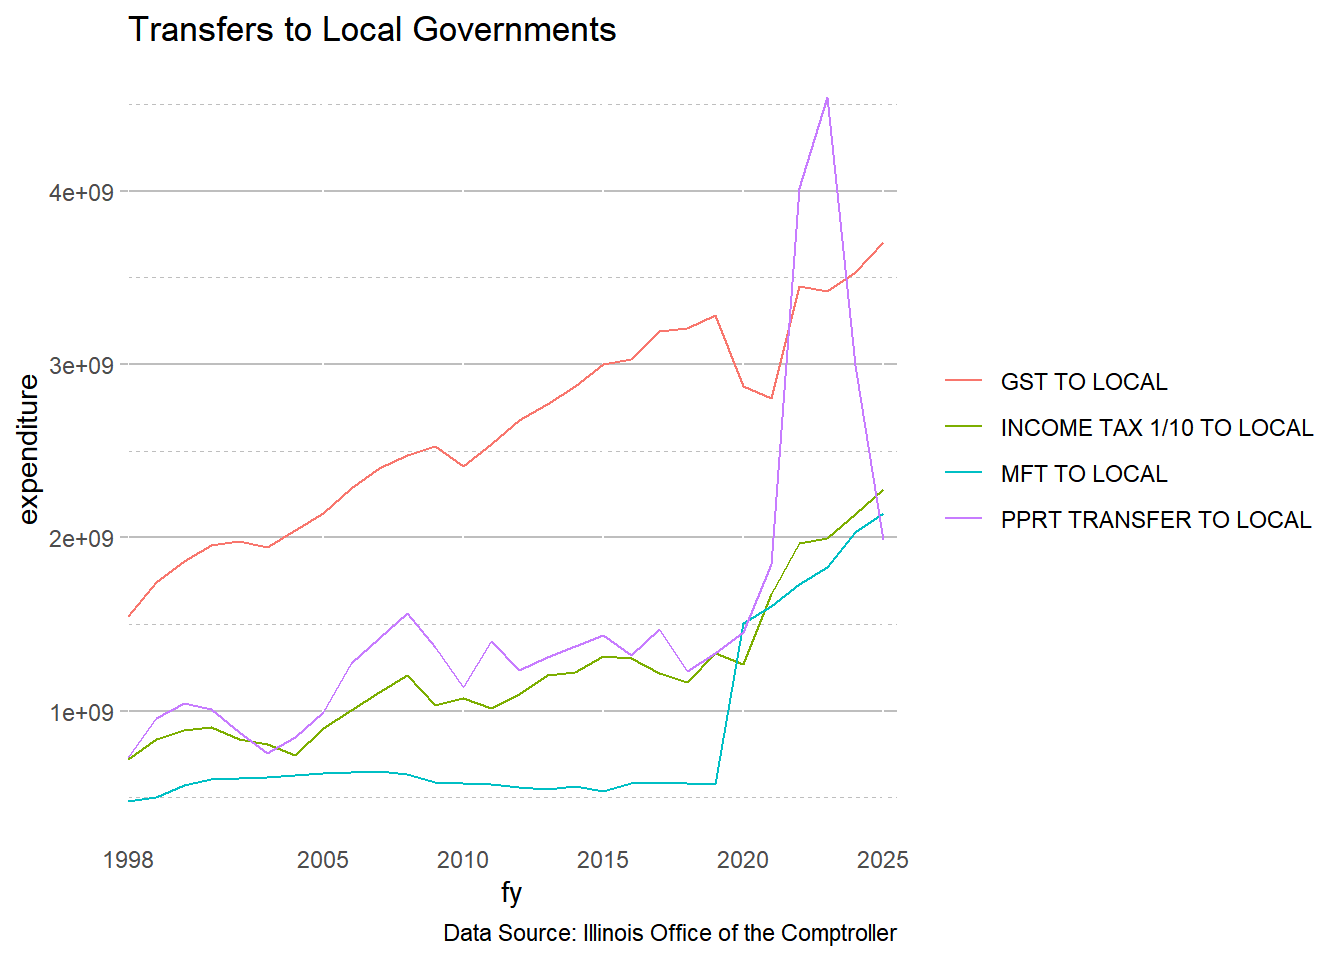
\includegraphics{./LocalTransfers_files/figure-pdf/graph-local-transfers-1.pdf}

}

\end{figure}

Large increases in local transfers were driven by large increases in
overall tax revenue collected by the state.

\bookmarksetup{startatroot}

\hypertarget{debt-service-discussion}{%
\chapter{Debt Service Discussion}\label{debt-service-discussion}}

\begin{Shaded}
\begin{Highlighting}[]
\FunctionTok{library}\NormalTok{(tidyverse)}
\FunctionTok{library}\NormalTok{(haven)}
\FunctionTok{library}\NormalTok{(formatR)}
\FunctionTok{library}\NormalTok{(lubridate)}
\FunctionTok{library}\NormalTok{(smooth)}
\FunctionTok{library}\NormalTok{(forecast)}
\FunctionTok{library}\NormalTok{(scales)}
\FunctionTok{library}\NormalTok{(kableExtra)}
\FunctionTok{library}\NormalTok{(ggplot2)}
\FunctionTok{library}\NormalTok{(readxl)}
\FunctionTok{library}\NormalTok{(tidyverse)}
\FunctionTok{library}\NormalTok{(data.table)}
\FunctionTok{library}\NormalTok{(quantmod)}
\FunctionTok{library}\NormalTok{(geofacet)}
\FunctionTok{library}\NormalTok{(janitor)}


\NormalTok{knitr}\SpecialCharTok{::}\NormalTok{opts\_chunk}\SpecialCharTok{$}\FunctionTok{set}\NormalTok{(}\AttributeTok{echo =} \ConstantTok{TRUE}\NormalTok{, }\AttributeTok{warning =} \ConstantTok{FALSE}\NormalTok{, }\AttributeTok{message =} \ConstantTok{FALSE}\NormalTok{)}

\NormalTok{exp\_temp }\OtherTok{\textless{}{-}} \FunctionTok{read\_csv}\NormalTok{(}\StringTok{"exp\_temp.csv"}\NormalTok{) }\SpecialCharTok{\%\textgreater{}\%} 
  \FunctionTok{filter}\NormalTok{(agency }\SpecialCharTok{!=} \StringTok{"799"}\NormalTok{) }

\NormalTok{rev\_temp }\OtherTok{\textless{}{-}} \FunctionTok{read\_csv}\NormalTok{(}\StringTok{"rev\_temp.csv"}\NormalTok{) }\SpecialCharTok{\%\textgreater{}\%} 
  \FunctionTok{filter}\NormalTok{(agency }\SpecialCharTok{!=} \StringTok{"799"}\NormalTok{)}
\end{Highlighting}
\end{Shaded}

Debt Service expenditures include interest payment on both short-term
and long-term debt. We do not include escrow or principal payments. Bond
proceeds are not considered a revenue for the state.

\textbf{Methodological Change, Sept.~30 2022:} We are no longer
including short term principal payments as a cost; only interest on
borrowing is a cost. Pre FY22 and the FY21 correction, we did include an
escrow payment and principle payments as costs but not bond proceeds as
revenues. This caused expenditures to be inflated because we were
essentially counting debt twice - the principle payment and whatever the
money was spent on in other expenditure categories, which was incorrect.

\hypertarget{coding-details}{%
\subsection{Coding Details}\label{coding-details}}

\textbf{Expenditure Debt Objects:}

\begin{itemize}
\tightlist
\item
  8811 is for principle payments \textbf{EXCLUDE}

  \begin{itemize}
  \tightlist
  \item
    General principle payments: obj\_seq\_type == 88110008
  \item
    Short term borrowing principle: obj\_seq\_type == 88110108
  \end{itemize}
\item
  8813 interest payments \textbf{INCLUDE AS COST}

  \begin{itemize}
  \tightlist
  \item
    General Obligation Bond Interest: obj\_seq\_type == 88130000 \&
    88130008
  \item
    Interest on short-term borrowing: 88130108
  \end{itemize}
\item
  8841 is for escrow payments \textbf{EXCLUDE}

  \begin{itemize}
  \tightlist
  \item
    Escrow payment: obj\_seq\_type == 88410008
  \end{itemize}
\item
  8800 is for all capital projects debt service (e.g.~Build Illinois
  Bonds, Civic Center) \textbf{INCLUDE AS COST}

  \begin{itemize}
  \tightlist
  \item
    \emph{Note: debt principle and interest are both included in capital
    projects because they are combined in the data observations; bond
    proceeds are not considered a revenue source. Can't include capital
    projects interest as easily as the GO bonds.}
  \item
    Build IL Bonds, capital projects principal AND interest (object
    ==8800)
  \end{itemize}
\item
  Tollway fund 0455 \textbf{EXCLUDE in debt cost}

  \begin{itemize}
  \tightlist
  \item
    Either filter out Tollway obj\_seq\_type == 88000055 or filter out
    fund == 0455 to remove tollway fund items from capital project debt
    service
  \end{itemize}
\end{itemize}

\hypertarget{state-principal-and-interest}{%
\subsubsection{State Principal and
Interest}\label{state-principal-and-interest}}

Filtering for interest on short term borrowing and GO bonds (88130008,
88130000, and 88130108) and GO bond principal amounts (88110008). Object
== 8813 is for all debt service interest but obj\_seq\_type is used to
specify short term borrowing versus regular debt service. An Interest to
Principal ratio is also calculated in the table below.

Looking only at general obligation principal payments and interest
payments:

\begin{Shaded}
\begin{Highlighting}[]
\CommentTok{\# GO bond principal and GO bond interest}

\NormalTok{GObond\_debt }\OtherTok{\textless{}{-}}\NormalTok{ exp\_temp }\SpecialCharTok{\%\textgreater{}\%} 
  \FunctionTok{filter}\NormalTok{(obj\_seq\_type }\SpecialCharTok{==} \StringTok{"88110008"} \SpecialCharTok{|}\NormalTok{obj\_seq\_type }\SpecialCharTok{==} \StringTok{"88130000"} \SpecialCharTok{|}\NormalTok{ obj\_seq\_type }\SpecialCharTok{==} \StringTok{"88130008"}\NormalTok{) }\SpecialCharTok{\%\textgreater{}\%} 
  \FunctionTok{group\_by}\NormalTok{(fy, obj\_seq\_type) }\SpecialCharTok{\%\textgreater{}\%} 
  \FunctionTok{summarize}\NormalTok{(}\AttributeTok{sum =} \FunctionTok{sum}\NormalTok{(expenditure, }\AttributeTok{na.rm=}\ConstantTok{FALSE}\NormalTok{)) }\SpecialCharTok{\%\textgreater{}\%} 
  \FunctionTok{pivot\_wider}\NormalTok{(}\AttributeTok{names\_from =}\NormalTok{ obj\_seq\_type, }\AttributeTok{values\_from =}\NormalTok{ sum) }\SpecialCharTok{\%\textgreater{}\%} 
  \FunctionTok{mutate}\NormalTok{(}\AttributeTok{principal =} \StringTok{\textasciigrave{}}\AttributeTok{88110008}\StringTok{\textasciigrave{}}\NormalTok{,}
         \AttributeTok{interest =} \FunctionTok{sum}\NormalTok{(}\StringTok{\textasciigrave{}}\AttributeTok{88130008}\StringTok{\textasciigrave{}}\SpecialCharTok{+}\StringTok{\textasciigrave{}}\AttributeTok{88130000}\StringTok{\textasciigrave{}}\NormalTok{, }\AttributeTok{na.rm =} \ConstantTok{FALSE}\NormalTok{),}
         \AttributeTok{ratio =}\NormalTok{ (}\FunctionTok{as.numeric}\NormalTok{(interest)}\SpecialCharTok{/}\FunctionTok{as.numeric}\NormalTok{(principal)))}

\NormalTok{GObond\_debt }\SpecialCharTok{\%\textgreater{}\%} 
  \FunctionTok{select}\NormalTok{(principal, interest, ratio) }\SpecialCharTok{\%\textgreater{}\%}
  \FunctionTok{mutate}\NormalTok{(}\FunctionTok{across}\NormalTok{(principal}\SpecialCharTok{:}\NormalTok{interest, }\SpecialCharTok{\textasciitilde{}}\FunctionTok{format}\NormalTok{(., }\AttributeTok{big.mark=} \StringTok{","}\NormalTok{, }\AttributeTok{scientific =}\NormalTok{ F)))}
\end{Highlighting}
\end{Shaded}

\begin{verbatim}
# A tibble: 25 x 4
# Groups:   fy [25]
      fy principal     interest       ratio
   <dbl> <chr>         <chr>          <dbl>
 1  1998 148,066,200   259,385,877     1.75
 2  1999 2,999,040     267,956,231    89.3 
 3  2000 1,000,000     287,154,654   287.  
 4  2001 154,166,026   NA             NA   
 5  2002 271,518,687   NA             NA   
 6  2003 138,351,231   NA             NA   
 7  2004 21,400,000    997,469,105    46.6 
 8  2005 37,400,000    1,061,205,268  28.4 
 9  2006 1,000,000,000 1,113,124,277   1.11
10  2007 6,995,000     1,115,485,186 159.  
# ... with 15 more rows
\end{verbatim}

\begin{Shaded}
\begin{Highlighting}[]
\CommentTok{\# GObond\_debt \%\textgreater{}\% ggplot() + }
\CommentTok{\#   geom\_line(aes(x=fy, y=principal, color = "Principal"))+ }
\CommentTok{\#   geom\_line(aes(x=fy, y=interest, color = "Interest")) + }
\CommentTok{\#   labs(title = "General Obligation principal and interest payments")}



\NormalTok{GObond\_debt }\SpecialCharTok{\%\textgreater{}\%} 
  \FunctionTok{ggplot}\NormalTok{() }\SpecialCharTok{+}   
    \FunctionTok{geom\_col}\NormalTok{(}\FunctionTok{aes}\NormalTok{(}\AttributeTok{x=}\NormalTok{fy, }\AttributeTok{y=}\NormalTok{interest}\SpecialCharTok{/}\DecValTok{1000000}\NormalTok{, }\AttributeTok{fill =} \StringTok{"Interest"}\NormalTok{)) }\SpecialCharTok{+} 
    \FunctionTok{geom\_col}\NormalTok{(}\FunctionTok{aes}\NormalTok{(}\AttributeTok{x=}\NormalTok{fy, }\AttributeTok{y=}\NormalTok{principal}\SpecialCharTok{/}\DecValTok{1000000}\NormalTok{, }\AttributeTok{fill =} \StringTok{"Principal"}\NormalTok{))}\SpecialCharTok{+} 
    \FunctionTok{labs}\NormalTok{(}\AttributeTok{title =} \StringTok{"Debt Service"}\NormalTok{, }
         \AttributeTok{subtitle =} \StringTok{"General Obligation Principal and Interest Payments"}\NormalTok{)}
\end{Highlighting}
\end{Shaded}

\begin{figure}[H]

{\centering \includegraphics{./Debt_files/figure-pdf/unnamed-chunk-2-1.pdf}

}

\end{figure}

Looking only at short term borrowing principal and interest payments:

\begin{Shaded}
\begin{Highlighting}[]
\CommentTok{\# short term borrowing, first observation is in 2004?}

\NormalTok{short\_debt }\OtherTok{\textless{}{-}}\NormalTok{ exp\_temp }\SpecialCharTok{\%\textgreater{}\%} 
  \FunctionTok{filter}\NormalTok{(obj\_seq\_type }\SpecialCharTok{==} \DecValTok{88110108} \SpecialCharTok{|}\NormalTok{obj\_seq\_type }\SpecialCharTok{==} \DecValTok{88130108}\NormalTok{) }\SpecialCharTok{\%\textgreater{}\%} 
  \FunctionTok{group\_by}\NormalTok{(fy, obj\_seq\_type) }\SpecialCharTok{\%\textgreater{}\%} 
  \FunctionTok{summarize}\NormalTok{(}\AttributeTok{sum =} \FunctionTok{sum}\NormalTok{(expenditure, }\AttributeTok{na.rm=}\ConstantTok{FALSE}\NormalTok{)) }\SpecialCharTok{\%\textgreater{}\%} 
  \FunctionTok{pivot\_wider}\NormalTok{(}\AttributeTok{names\_from =}\NormalTok{ obj\_seq\_type, }\AttributeTok{values\_from =}\NormalTok{ sum) }\SpecialCharTok{\%\textgreater{}\%} 
  \FunctionTok{mutate}\NormalTok{(}\AttributeTok{principal =} \StringTok{\textasciigrave{}}\AttributeTok{88110108}\StringTok{\textasciigrave{}}\NormalTok{,}
         \AttributeTok{interest =} \StringTok{\textasciigrave{}}\AttributeTok{88130108}\StringTok{\textasciigrave{}}\NormalTok{,}
         \AttributeTok{ratio =}\NormalTok{ (}\FunctionTok{as.numeric}\NormalTok{(interest)}\SpecialCharTok{/}\FunctionTok{as.numeric}\NormalTok{(principal)))}

\NormalTok{short\_debt }\SpecialCharTok{\%\textgreater{}\%} \FunctionTok{select}\NormalTok{(principal, interest, ratio) }\SpecialCharTok{\%\textgreater{}\%}
  \FunctionTok{mutate}\NormalTok{(}\FunctionTok{across}\NormalTok{(principal}\SpecialCharTok{:}\NormalTok{interest, }\SpecialCharTok{\textasciitilde{}}\FunctionTok{format}\NormalTok{(., }\AttributeTok{big.mark=} \StringTok{","}\NormalTok{,  }\AttributeTok{scientific =}\NormalTok{ F)))}
\end{Highlighting}
\end{Shaded}

\begin{verbatim}
# A tibble: 9 x 4
# Groups:   fy [9]
     fy principal     interest      ratio
  <dbl> <chr>         <chr>         <dbl>
1  2004 1,500,000,000 22,364,583  0.0149 
2  2005 1,615,000,000 10,672,222  0.00661
3  2007 900,000,000   NA         NA      
4  2008 1,200,000,000 6,233,333   0.00519
5  2009 1,400,000,000 26,675,000  0.0191 
6  2010 2,250,000,000 55,277,778  0.0246 
7  2011 1,300,000,000 30,975,000  0.0238 
8  2021 2,184,745,000 51,007,557  0.0233 
9  2022 1,164,255,000 90,437,183  0.0777 
\end{verbatim}

\begin{Shaded}
\begin{Highlighting}[]
\NormalTok{short\_debt }\SpecialCharTok{\%\textgreater{}\%} \FunctionTok{ggplot}\NormalTok{() }\SpecialCharTok{+} 
  \FunctionTok{geom\_col}\NormalTok{(}\FunctionTok{aes}\NormalTok{(}\AttributeTok{x=}\NormalTok{fy, }\AttributeTok{y=}\NormalTok{principal}\SpecialCharTok{/}\DecValTok{1000000000}\NormalTok{, }\AttributeTok{fill =} \StringTok{"Principal"}\NormalTok{))}\SpecialCharTok{+} 
  \FunctionTok{geom\_col}\NormalTok{(}\FunctionTok{aes}\NormalTok{(}\AttributeTok{x=}\NormalTok{fy, }\AttributeTok{y=}\NormalTok{interest}\SpecialCharTok{/}\DecValTok{1000000000}\NormalTok{, }\AttributeTok{fill =} \StringTok{"Interest"}\NormalTok{)) }\SpecialCharTok{+} 
  \FunctionTok{labs}\NormalTok{(}\AttributeTok{title =} \StringTok{"Debt Service"}\NormalTok{, }\AttributeTok{subtitle =} \StringTok{"Short Term Borrowing: Principal and Interest Payments"}\NormalTok{, }\AttributeTok{y=}\StringTok{"Billions of Dollars"}\NormalTok{)}
\end{Highlighting}
\end{Shaded}

\begin{figure}[H]

{\centering 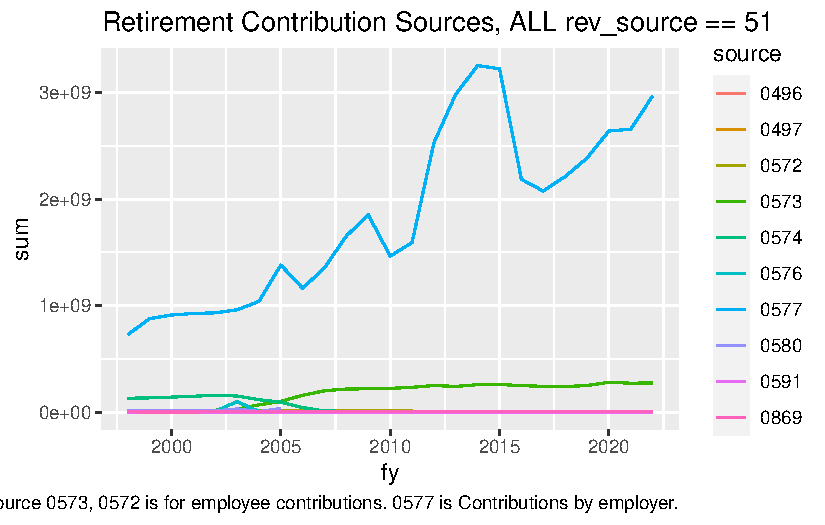
\includegraphics{./Debt_files/figure-pdf/unnamed-chunk-3-1.pdf}

}

\end{figure}

\begin{quote}
When including short term borrowing and normal debt service together,
the debt ratio seems more c anonsistent d the total interest and
principal payments over the years are smoothed out.
\end{quote}

Debt service for Capital projects (object==8800) is examined below.
Tollway debt service is EXCLUDED from these values. The ratio calculated
in the table below is interest/principal.

\begin{Shaded}
\begin{Highlighting}[]
\NormalTok{capitalprojects }\OtherTok{\textless{}{-}}\NormalTok{ exp\_temp }\SpecialCharTok{\%\textgreater{}\%} 
  \FunctionTok{filter}\NormalTok{(object }\SpecialCharTok{==} \StringTok{"8800"} \SpecialCharTok{\&}\NormalTok{ fund }\SpecialCharTok{!=} \StringTok{"0455"}\NormalTok{) }\CommentTok{\# capital debt service except tollway}

\NormalTok{all\_debt }\OtherTok{\textless{}{-}}\NormalTok{ exp\_temp }\SpecialCharTok{\%\textgreater{}\%}     \CommentTok{\# all principal, interest, and debt service except Tollway}
  \FunctionTok{filter}\NormalTok{(fund }\SpecialCharTok{!=} \StringTok{"0455"} \SpecialCharTok{\&}\NormalTok{ (object }\SpecialCharTok{==} \StringTok{"8811"} \SpecialCharTok{|}\NormalTok{object }\SpecialCharTok{==} \StringTok{"8813"} \SpecialCharTok{|}\NormalTok{ object }\SpecialCharTok{==} \StringTok{"8800"}\NormalTok{) )}\SpecialCharTok{\%\textgreater{}\%} 
  \FunctionTok{group\_by}\NormalTok{(fy, object) }\SpecialCharTok{\%\textgreater{}\%} 
  \FunctionTok{summarize}\NormalTok{(}\AttributeTok{sum =} \FunctionTok{sum}\NormalTok{(expenditure, }\AttributeTok{na.rm=}\ConstantTok{TRUE}\NormalTok{)) }\SpecialCharTok{\%\textgreater{}\%} 
  \FunctionTok{pivot\_wider}\NormalTok{(}\AttributeTok{names\_from =}\NormalTok{ object, }\AttributeTok{values\_from =}\NormalTok{ sum) }\SpecialCharTok{\%\textgreater{}\%} 
  \FunctionTok{mutate}\NormalTok{(}\AttributeTok{principal =} \StringTok{\textasciigrave{}}\AttributeTok{8811}\StringTok{\textasciigrave{}}\NormalTok{,}
         \AttributeTok{interest =} \StringTok{\textasciigrave{}}\AttributeTok{8813}\StringTok{\textasciigrave{}}\NormalTok{,}
         \AttributeTok{CapitalProjects =} \StringTok{\textasciigrave{}}\AttributeTok{8800}\StringTok{\textasciigrave{}}\NormalTok{,}
         \AttributeTok{ratio =}\NormalTok{ (}\FunctionTok{as.numeric}\NormalTok{(interest)}\SpecialCharTok{/}\FunctionTok{as.numeric}\NormalTok{(principal)))}

\NormalTok{all\_debt }\SpecialCharTok{\%\textgreater{}\%} 
  \FunctionTok{select}\NormalTok{(principal, interest, CapitalProjects, ratio) }\SpecialCharTok{\%\textgreater{}\%}
  \FunctionTok{mutate}\NormalTok{(}\FunctionTok{across}\NormalTok{(principal}\SpecialCharTok{:}\NormalTok{CapitalProjects, }\SpecialCharTok{\textasciitilde{}}\FunctionTok{format}\NormalTok{(., }\AttributeTok{big.mark=} \StringTok{","}\NormalTok{, }\AttributeTok{scientific =}\NormalTok{ F)))}
\end{Highlighting}
\end{Shaded}

\begin{verbatim}
# A tibble: 25 x 5
# Groups:   fy [25]
      fy principal     interest      CapitalProjects ratio
   <dbl> <chr>         <chr>         <chr>           <dbl>
 1  1998 575,371,231   259,385,877   225,148,458     0.451
 2  1999 422,975,040   267,956,231   239,571,392     0.634
 3  2000 430,464,406   287,154,654   256,685,875     0.667
 4  2001 585,553,477   336,582,816   253,461,423     0.575
 5  2002 740,370,036   382,634,975   257,622,074     0.517
 6  2003 1,658,569,732 474,937,865   256,264,319     0.286
 7  2004 1,923,668,657 1,019,833,688 268,750,574     0.530
 8  2005 2,153,260,524 1,071,877,490 279,939,826     0.498
 9  2006 1,565,449,887 1,113,124,277 302,328,995     0.711
10  2007 1,477,592,635 1,115,485,186 301,723,144     0.755
# ... with 15 more rows
\end{verbatim}

\begin{Shaded}
\begin{Highlighting}[]
\NormalTok{all\_debt }\SpecialCharTok{\%\textgreater{}\%} 
  \FunctionTok{ggplot}\NormalTok{() }\SpecialCharTok{+} 
    \FunctionTok{geom\_line}\NormalTok{(}\FunctionTok{aes}\NormalTok{(}\AttributeTok{x=}\NormalTok{fy, }\AttributeTok{y=}\NormalTok{principal}\SpecialCharTok{/}\DecValTok{1000000}\NormalTok{, }\AttributeTok{color =} \StringTok{"Principal"}\NormalTok{))}\SpecialCharTok{+} 
    \FunctionTok{geom\_line}\NormalTok{(}\FunctionTok{aes}\NormalTok{(}\AttributeTok{x=}\NormalTok{fy, }\AttributeTok{y=}\NormalTok{interest}\SpecialCharTok{/}\DecValTok{1000000}\NormalTok{, }\AttributeTok{color =} \StringTok{"Interest"}\NormalTok{))}\SpecialCharTok{+}
    \FunctionTok{geom\_line}\NormalTok{(}\FunctionTok{aes}\NormalTok{(}\AttributeTok{x=}\NormalTok{fy, }\AttributeTok{y =}\NormalTok{ CapitalProjects }\SpecialCharTok{/} \DecValTok{1000000}\NormalTok{, }\AttributeTok{color =} \StringTok{"Capital Projects"}\NormalTok{))}\SpecialCharTok{+}
    \FunctionTok{labs}\NormalTok{(}\AttributeTok{y =} \StringTok{"Debt ($Millions)"}\NormalTok{,}
         \AttributeTok{title =} \StringTok{"Illinois Principal and Interest payments"}\NormalTok{, }
         \AttributeTok{subtitle =} \StringTok{"Principal and interest from short term borrowing and GO Bonds debt service"}\NormalTok{, }
         \AttributeTok{caption =} \StringTok{"Capital projects does not include Illinois tollway debt service.}
\StringTok{         Capital projects data include interest and principal values as one value and is graphed separately."}\NormalTok{)}
\end{Highlighting}
\end{Shaded}

\begin{figure}[H]

{\centering \includegraphics{./Debt_files/figure-pdf/unnamed-chunk-4-1.pdf}

}

\end{figure}

\hypertarget{section-1}{%
\subsubsection{}\label{section-1}}

For additional context on bond proceeds coming in compared to the debt
service being paid, here is a very simple graph of all bond proceeds.
Bond proceeds are not considered a revenue source in the Fiscal Futures
model. We do not dive into the different types of proceeds but that
could be an interesting topic by itself.

\begin{Shaded}
\begin{Highlighting}[]
\NormalTok{rev\_temp }\SpecialCharTok{\%\textgreater{}\%} 
  \FunctionTok{filter}\NormalTok{(rev\_type }\SpecialCharTok{==} \StringTok{"72"}\NormalTok{)}
\end{Highlighting}
\end{Shaded}

\begin{verbatim}
# A tibble: 213 x 29
      fy fund  agency source interfund_trans from_fund source_name      receipts
   <dbl> <chr>  <dbl> <chr>            <dbl> <chr>     <chr>               <dbl>
 1  1998 0101     370 0571                 0 .         BOND ISSUE PROC~   1.23e8
 2  1998 0141     370 0571                 0 .         BOND ISSUE PROC~   5.16e8
 3  1998 0551     370 0571                 0 .         BOND ISSUE PROC~   2.97e7
 4  1998 0554     370 0571                 0 .         BOND ISSUE PROC~   4.66e7
 5  1998 0556     370 0571                 0 .         BOND ISSUE PROC~   3.74e7
 6  1998 0653     370 0571                 0 .         BOND ISSUE PROC~   5.02e6
 7  1998 0971     370 0571                 0 .         BOND ISSUE PROC~   1.48e8
 8  1999 0101     370 0571                 0 .         BOND ISSUE PROC~   1.73e8
 9  1999 0141     370 0571                 0 .         BOND ISSUE PROC~   4.21e8
10  1999 0143     370 0571                 0 .         BOND ISSUE PROC~   1.20e8
# ... with 203 more rows, and 21 more variables: data_source <chr>,
#   fund_name <chr>, agency_name <chr>, fund_cat <chr>, fund_cat_name.x <chr>,
#   fund_ab <chr>, fund_ioc <chr>, fund_re <dbl>, a_end <dbl>, in_ff <dbl>,
#   fund_name_ab <chr>, fund_category <chr>, fund_cat_name.y <chr>,
#   in_ff_rev <dbl>, in_ff_exp <dbl>, source_name_AWM <chr>, rev_type <chr>,
#   rev_type_name <chr>, amnesty <lgl>, local <dbl>, type_assigned <dbl>
\end{verbatim}

\begin{Shaded}
\begin{Highlighting}[]
\NormalTok{bond\_proceeds }\OtherTok{\textless{}{-}}\NormalTok{ rev\_temp }\SpecialCharTok{\%\textgreater{}\%} 
  \FunctionTok{filter}\NormalTok{(rev\_type }\SpecialCharTok{==} \StringTok{"72"}\NormalTok{) }\SpecialCharTok{\%\textgreater{}\%} \CommentTok{\#bond proceeds}
\CommentTok{\#  filter(agency == "370" \& source == "0571") \%\textgreater{}\%     }
  \FunctionTok{group\_by}\NormalTok{(fy, fund\_cat\_name.y) }\SpecialCharTok{\%\textgreater{}\%} 
  \FunctionTok{summarize}\NormalTok{(}\AttributeTok{sum =} \FunctionTok{sum}\NormalTok{(receipts}\SpecialCharTok{/}\DecValTok{1000000000}\NormalTok{, }\AttributeTok{na.rm=}\ConstantTok{FALSE}\NormalTok{))}

\NormalTok{rev\_temp }\SpecialCharTok{\%\textgreater{}\%} \FunctionTok{filter}\NormalTok{(rev\_type }\SpecialCharTok{==} \StringTok{"72"}\NormalTok{) }\SpecialCharTok{\%\textgreater{}\%} \FunctionTok{ggplot}\NormalTok{() }\SpecialCharTok{+} \FunctionTok{geom\_col}\NormalTok{(}\FunctionTok{aes}\NormalTok{(}\AttributeTok{x=}\NormalTok{fy, }\AttributeTok{y=}\NormalTok{receipts)) }\SpecialCharTok{+} \FunctionTok{labs}\NormalTok{(}\AttributeTok{title =} \StringTok{"All Bond Proceeds"}\NormalTok{)}
\end{Highlighting}
\end{Shaded}

\begin{figure}[H]

{\centering 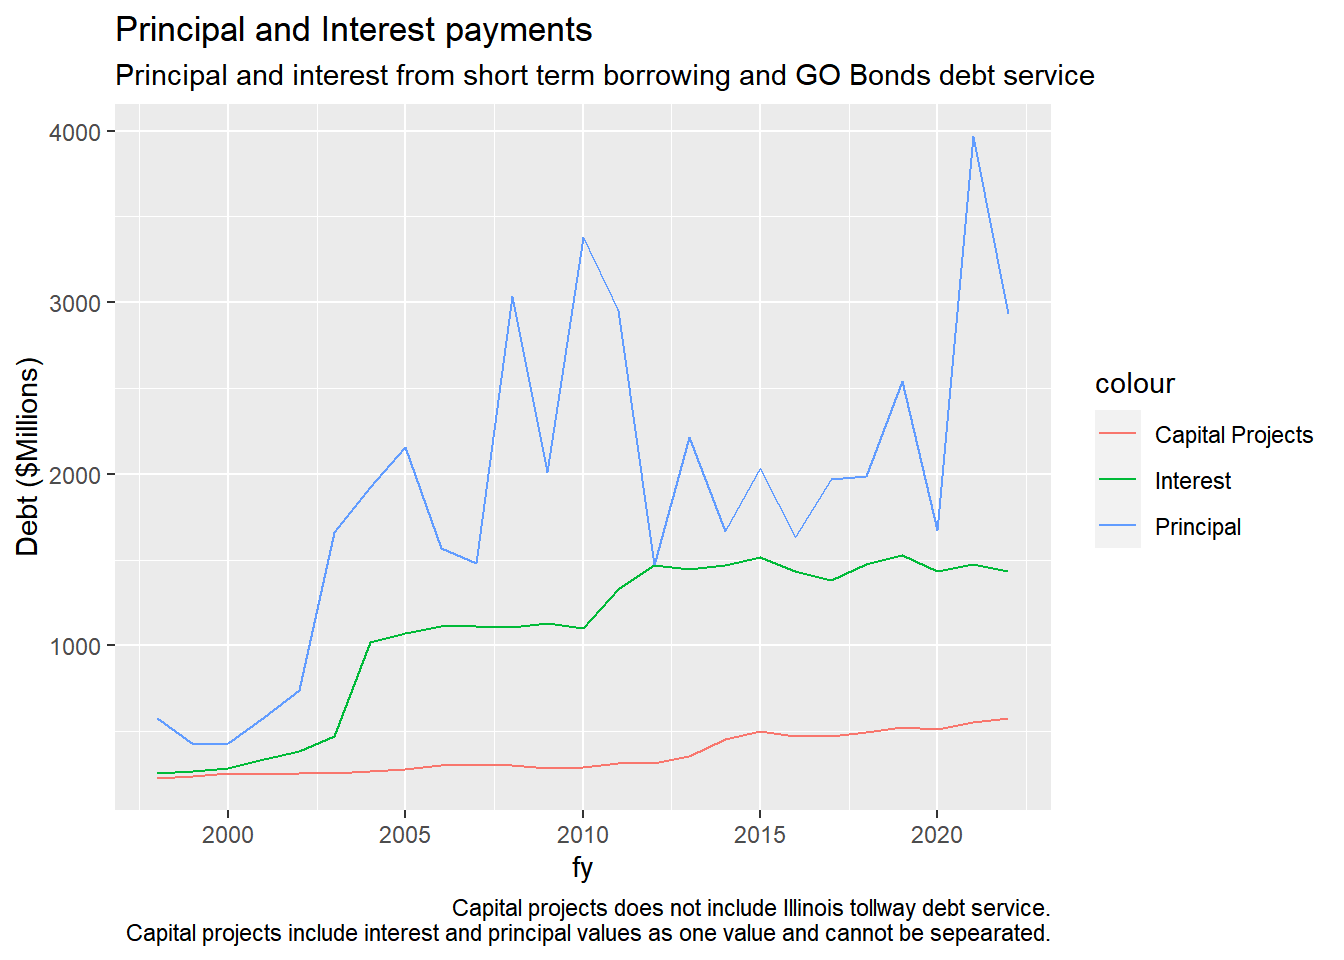
\includegraphics{./Debt_files/figure-pdf/unnamed-chunk-5-1.pdf}

}

\end{figure}

\begin{Shaded}
\begin{Highlighting}[]
\NormalTok{bond\_proceeds }\SpecialCharTok{\%\textgreater{}\%} \FunctionTok{ggplot}\NormalTok{() }\SpecialCharTok{+} 
  \FunctionTok{geom\_line}\NormalTok{(}\FunctionTok{aes}\NormalTok{(}\AttributeTok{x=}\NormalTok{fy, }\AttributeTok{y=}\NormalTok{sum, }\AttributeTok{color=}\NormalTok{fund\_cat\_name.y)) }\SpecialCharTok{+} 
  \FunctionTok{labs}\NormalTok{(}\AttributeTok{title =} \StringTok{"Bond Proceeds, Revenue Type = 72"}\NormalTok{, }\AttributeTok{y=}\StringTok{"Billions of Dollars"}\NormalTok{)}
\end{Highlighting}
\end{Shaded}

\begin{figure}[H]

{\centering 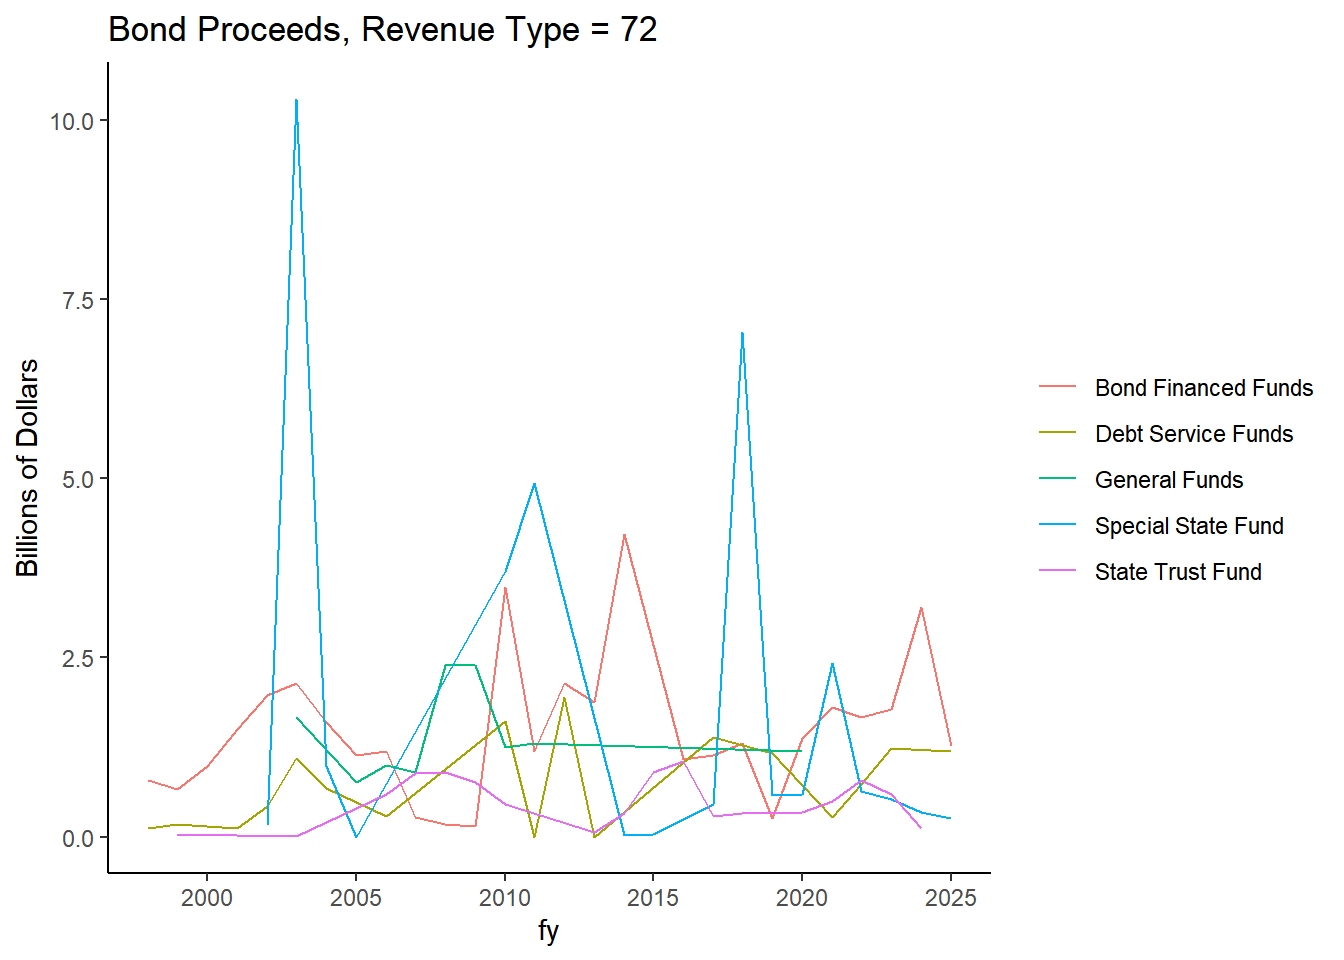
\includegraphics{./Debt_files/figure-pdf/unnamed-chunk-5-2.pdf}

}

\end{figure}

\hypertarget{tollway-debt-revenue-and-expenditures}{%
\subsubsection{Tollway Debt, Revenue, and
Expenditures}\label{tollway-debt-revenue-and-expenditures}}

A note on what is considered Transportation vs.~Tollway vs.~Capital
Projects:

\begin{itemize}
\tightlist
\item
  Transportation costs is made up of the road fund (0011) , capital
  administrative costs, and maintenance costs for the agency=494,
  Department of Transportation.
\item
  Tollway expenditures include maintenance and operation, principle and
  interest payments occurring from fund 0455 and agency = 577.
\item
  Capital improvement has a lot of projects that use bond financed funds
  for schools, sports facilities, etc. Agencies 511, 554, 574, and 598
  are coded together as group 946, capital improvement (Capital
  Development Board, Sports Facilities Development Authority, Metro Pier
  and Exposition Authority, and Upper River Development Authority which
  is no longer used). IOC uses object 8800.
\end{itemize}

\emph{Coding Notes: Filtering by Tollway agency 577 expenditures = SAME
as filtering by fund == 0455 expenditures}

\begin{itemize}
\tightlist
\item
  Total Tollway expenditure = Debt service costs + maintenance \&
  operation costs
\end{itemize}

Principal and interest amounts calculated for the state exclude the
Illinois Tollway debt service and debt service for capital projects
(mostly because principal and interest are included as one item in the
data). Examples of capital projects include the IL Civic Center and
Build Illinois Bonds. Tollway principal and interest IS included in the
Illinois Tollway expenditures.

The object \texttt{tollway} includes all Tollway expenditures (capital
improvements, principal and interest payments, operations, etc).

\begin{Shaded}
\begin{Highlighting}[]
\CommentTok{\# exp\_temp \%\textgreater{}\% }
\CommentTok{\#   filter(fund == "0455") \%\textgreater{}\%       \# tollway fund}
\CommentTok{\#   group\_by(fy) \%\textgreater{}\% }
\CommentTok{\#   summarize(sum = sum(expenditure)) \%\textgreater{}\% }
\CommentTok{\#   arrange({-}fy)}

\NormalTok{alltollway\_exp }\OtherTok{\textless{}{-}}\NormalTok{ exp\_temp }\SpecialCharTok{\%\textgreater{}\%} 
  \FunctionTok{filter}\NormalTok{(fund }\SpecialCharTok{==} \StringTok{"0455"}\NormalTok{) }\SpecialCharTok{\%\textgreater{}\%} \CommentTok{\# all tollway expenditures, including debt service}
  \FunctionTok{group\_by}\NormalTok{(fy) }\SpecialCharTok{\%\textgreater{}\%} 
  \FunctionTok{summarize}\NormalTok{(}\AttributeTok{expenditure =} \FunctionTok{sum}\NormalTok{(expenditure))}
\NormalTok{alltollway\_exp}
\end{Highlighting}
\end{Shaded}

\begin{verbatim}
# A tibble: 25 x 2
      fy expenditure
   <dbl>       <dbl>
 1  1998  367420329.
 2  1999  461112230.
 3  2000  434678650.
 4  2001  346139195.
 5  2002  392743878.
 6  2003  360732939.
 7  2004  417188659.
 8  2005  479320182.
 9  2006 1073754714.
10  2007 1432879386.
# ... with 15 more rows
\end{verbatim}

\begin{Shaded}
\begin{Highlighting}[]
\NormalTok{tollway\_exp }\OtherTok{\textless{}{-}}\NormalTok{ exp\_temp }\SpecialCharTok{\%\textgreater{}\%} \CommentTok{\#expenditures without debt service}
  \FunctionTok{filter}\NormalTok{(fund }\SpecialCharTok{==} \StringTok{"0455"} \SpecialCharTok{\&}\NormalTok{ object }\SpecialCharTok{!=} \StringTok{"8800"}\NormalTok{) }\SpecialCharTok{\%\textgreater{}\%} 
  \FunctionTok{group\_by}\NormalTok{(fy) }\SpecialCharTok{\%\textgreater{}\%} 
  \FunctionTok{summarize}\NormalTok{(}\AttributeTok{expenditure =} \FunctionTok{sum}\NormalTok{(expenditure))}

\CommentTok{\#tollway debt principal and interest}
\NormalTok{tollwaydebt }\OtherTok{\textless{}{-}}\NormalTok{ exp\_temp }\SpecialCharTok{\%\textgreater{}\%}
  \FunctionTok{filter}\NormalTok{(object }\SpecialCharTok{==} \StringTok{"8800"} \SpecialCharTok{\&}\NormalTok{ fund }\SpecialCharTok{==} \StringTok{"0455"}\NormalTok{) }\SpecialCharTok{\%\textgreater{}\%} 
  \FunctionTok{group\_by}\NormalTok{(fy) }\SpecialCharTok{\%\textgreater{}\%} 
  \FunctionTok{summarize}\NormalTok{(}\AttributeTok{sum=}\FunctionTok{sum}\NormalTok{(expenditure)) }


\NormalTok{capitalproject\_debtservice }\OtherTok{\textless{}{-}}\NormalTok{ exp\_temp }\SpecialCharTok{\%\textgreater{}\%}
  \FunctionTok{filter}\NormalTok{(object }\SpecialCharTok{==} \StringTok{"8800"}\NormalTok{) }\CommentTok{\# ALL Capital projects debt service including tollway}

\CommentTok{\# look at Illinois tollway bond proceeds and debt service: }
\CommentTok{\# rev\_temp \%\textgreater{}\% filter(fund == "0455") \# examine revenue to fund 0455}


\NormalTok{alltollway\_rev }\OtherTok{\textless{}{-}}\NormalTok{ rev\_temp }\SpecialCharTok{\%\textgreater{}\%} 
  \FunctionTok{filter}\NormalTok{(fund }\SpecialCharTok{==} \StringTok{"0455"}\NormalTok{) }\SpecialCharTok{\%\textgreater{}\%}  \CommentTok{\# includes bond proceeds}
  \FunctionTok{group\_by}\NormalTok{(fy) }\SpecialCharTok{\%\textgreater{}\%} 
  \FunctionTok{summarize}\NormalTok{(}\AttributeTok{sum =} \FunctionTok{sum}\NormalTok{(receipts)) }\SpecialCharTok{\%\textgreater{}\%} 
  \FunctionTok{arrange}\NormalTok{(}\SpecialCharTok{{-}}\NormalTok{fy)}

\NormalTok{tollway\_rev }\OtherTok{\textless{}{-}}\NormalTok{ rev\_temp }\SpecialCharTok{\%\textgreater{}\%} \CommentTok{\#tollway revenue without bond proceeds}
  \FunctionTok{filter}\NormalTok{(fund }\SpecialCharTok{==} \StringTok{"0455"} \SpecialCharTok{\&}\NormalTok{ source }\SpecialCharTok{!=} \StringTok{"0571"}\NormalTok{) }\SpecialCharTok{\%\textgreater{}\%} 
  \FunctionTok{group\_by}\NormalTok{(fy) }\SpecialCharTok{\%\textgreater{}\%} 
  \FunctionTok{summarize}\NormalTok{(}\AttributeTok{sum =} \FunctionTok{sum}\NormalTok{(receipts, }\AttributeTok{na.rm =} \ConstantTok{TRUE}\NormalTok{))}



\CommentTok{\# tollway bond proceeds}
\NormalTok{tollway\_bondproc }\OtherTok{\textless{}{-}}\NormalTok{ rev\_temp }\SpecialCharTok{\%\textgreater{}\%} 
  \FunctionTok{filter}\NormalTok{(fund }\SpecialCharTok{==} \StringTok{"0455"} \SpecialCharTok{\&}\NormalTok{ source }\SpecialCharTok{==} \StringTok{"0571"}\NormalTok{ ) }\SpecialCharTok{\%\textgreater{}\%} 
  \FunctionTok{group\_by}\NormalTok{(fy) }\SpecialCharTok{\%\textgreater{}\%} 
  \FunctionTok{summarize}\NormalTok{(}\AttributeTok{sum =} \FunctionTok{sum}\NormalTok{(receipts, }\AttributeTok{na.rm =} \ConstantTok{TRUE}\NormalTok{))}

\CommentTok{\#alltollway \%\textgreater{}\%  ggplot() + geom\_line(aes(x=fy, y=sum)) + labs(title = "Fund 0455 {-} All Tollway Revenue", caption = "Data from IOC Revenue Files. Fund 0455 is the IL State Tollway Revenue") }

\CommentTok{\#tollway\_bondproc \%\textgreater{}\% ggplot() + geom\_line(aes(x=fy, y=sum)) + labs(title = "Fund 0455 {-} Tollway Revenue: Tollway Bond Proceeds", caption = "Data from IOC Revenue Files. Fund 0455 is the IL State Tollway Revenue")}

  

\CommentTok{\#ggplot() + geom\_line(data=tollway\_bondproc, aes(x=fy, y=sum)) + labs(title = "Fund 0455 {-} Tollway Revenue: Tollway Bond Proceeds", caption = "Data from IOC Revenue Files. Fund 0455 is the IL State Tollway Revenue")}

\CommentTok{\#tollwaydebt \%\textgreater{}\% ggplot() + geom\_line(aes(x=fy, y=sum)) + labs(title = "Tollway Debt Service", caption = "Debt service includes principal and interest for the Illinois Tollway. Object = 8800 and fund = 0455")}




\DocumentationTok{\#\# Tollway agency 577 expenditures = SAME as filtering by tollway fund == 0455 \#\#}

\CommentTok{\# tollway\textless{}{-}exp\_temp \%\textgreater{}\% filter(agency == "557")}

\CommentTok{\# exp\_temp \%\textgreater{}\% filter(agency == "557") \%\textgreater{}\% group\_by(fy) \%\textgreater{}\% summarize(sum = sum(expenditure)) \%\textgreater{}\% arrange({-}fy)}



\FunctionTok{ggplot}\NormalTok{()}\SpecialCharTok{+}
  \FunctionTok{geom\_col}\NormalTok{(}\AttributeTok{data=}\NormalTok{tollway\_bondproc, }\FunctionTok{aes}\NormalTok{(}\AttributeTok{x=}\NormalTok{fy, }\AttributeTok{y=}\NormalTok{sum)) }\SpecialCharTok{+}
  \FunctionTok{geom\_line}\NormalTok{(}\AttributeTok{data=}\NormalTok{ tollwaydebt, }\FunctionTok{aes}\NormalTok{(}\AttributeTok{x=}\NormalTok{fy, }\AttributeTok{y =}\NormalTok{ sum, }\AttributeTok{color =} \StringTok{\textquotesingle{}Debt Service\textquotesingle{}}\NormalTok{))}\SpecialCharTok{+} 
  \FunctionTok{geom\_line}\NormalTok{(}\AttributeTok{data=}\NormalTok{ tollway\_exp, }\FunctionTok{aes}\NormalTok{(}\AttributeTok{x=}\NormalTok{fy, }\AttributeTok{y =}\NormalTok{ expenditure, }\AttributeTok{color =} \StringTok{\textquotesingle{}Tollway Expenditures\textquotesingle{}}\NormalTok{))}\SpecialCharTok{+} 
  \FunctionTok{geom\_line}\NormalTok{(}\AttributeTok{data=}\NormalTok{ tollway\_rev, }\FunctionTok{aes}\NormalTok{(}\AttributeTok{x=}\NormalTok{fy, }\AttributeTok{y =}\NormalTok{ sum, }\AttributeTok{color =} \StringTok{"Tollway Revenue"}\NormalTok{))}\SpecialCharTok{+} 
  \FunctionTok{scale\_color\_manual}\NormalTok{(}\AttributeTok{values =} \FunctionTok{c}\NormalTok{(}
    \StringTok{\textquotesingle{}Bond Proceeds\textquotesingle{}} \OtherTok{=} \StringTok{\textquotesingle{}darkgray\textquotesingle{}}\NormalTok{,}
    \StringTok{\textquotesingle{}Debt Service\textquotesingle{}} \OtherTok{=} \StringTok{\textquotesingle{}red\textquotesingle{}}\NormalTok{,}
    \StringTok{\textquotesingle{}Tollway Expenditures\textquotesingle{}} \OtherTok{=} \StringTok{\textquotesingle{}orange\textquotesingle{}}\NormalTok{,}
    \StringTok{\textquotesingle{}Tollway Revenue\textquotesingle{}} \OtherTok{=} \StringTok{\textquotesingle{}light green\textquotesingle{}}\NormalTok{)) }\SpecialCharTok{+}
  \FunctionTok{labs}\NormalTok{(}\AttributeTok{title=}\StringTok{"Tollway bond procreeds, debt service, revenue, and expenditures."}\NormalTok{, }
       \AttributeTok{caption =} \StringTok{"Tollway revenue + bond proceeds should be roughly equal to tollway expenditures + debt service."}\NormalTok{, }
       \AttributeTok{y =} \StringTok{"Dollars"}\NormalTok{)}
\end{Highlighting}
\end{Shaded}

\begin{figure}[H]

{\centering 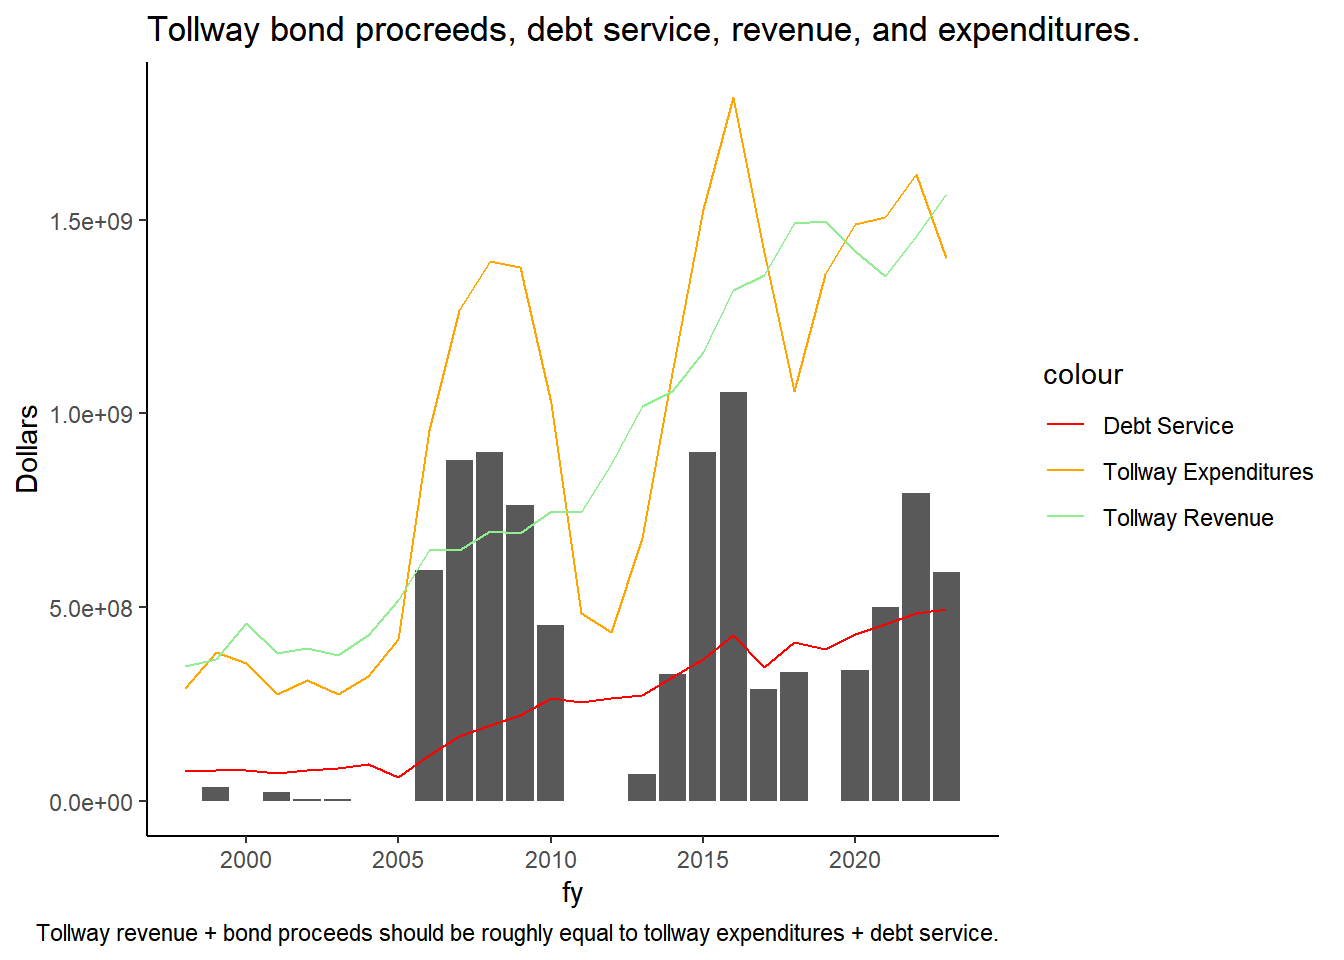
\includegraphics{./Debt_files/figure-pdf/tollway-1.pdf}

}

\end{figure}

\begin{Shaded}
\begin{Highlighting}[]
\FunctionTok{ggplot}\NormalTok{()}\SpecialCharTok{+}
  \FunctionTok{geom\_line}\NormalTok{(}\AttributeTok{data=}\NormalTok{alltollway\_exp, }\FunctionTok{aes}\NormalTok{(}\AttributeTok{x=}\NormalTok{fy, }\AttributeTok{y=}\NormalTok{expenditure}\SpecialCharTok{/}\DecValTok{1000000000}\NormalTok{, }\AttributeTok{color =} \StringTok{"All Tollway Revenue"}\NormalTok{)) }\SpecialCharTok{+}
  \FunctionTok{geom\_line}\NormalTok{(}\AttributeTok{data=}\NormalTok{ alltollway\_rev, }\FunctionTok{aes}\NormalTok{(}\AttributeTok{x=}\NormalTok{fy, }\AttributeTok{y =}\NormalTok{ sum}\SpecialCharTok{/}\DecValTok{1000000000}\NormalTok{, }\AttributeTok{color =} \StringTok{\textquotesingle{}All Tollway Expenditures\textquotesingle{}}\NormalTok{))}\SpecialCharTok{+} 
  \FunctionTok{scale\_color\_manual}\NormalTok{(}\AttributeTok{values =} \FunctionTok{c}\NormalTok{(}
    \StringTok{\textquotesingle{}All Tollway Revenue\textquotesingle{}} \OtherTok{=} \StringTok{\textquotesingle{}darkgray\textquotesingle{}}\NormalTok{,}
    \StringTok{\textquotesingle{}All Tollway Expenditures\textquotesingle{}} \OtherTok{=} \StringTok{\textquotesingle{}red\textquotesingle{}}\NormalTok{)) }\SpecialCharTok{+}
  \FunctionTok{theme}\NormalTok{(}\AttributeTok{legend.position =} \StringTok{"bottom"}\NormalTok{)}\SpecialCharTok{+}
  \FunctionTok{labs}\NormalTok{(}\AttributeTok{title=}\StringTok{" All revenues (Tolls + bond proceeds) and all expenditures (operations, capital improvements, \& debt service.)"}\NormalTok{, }
       \AttributeTok{caption =} \StringTok{"Tollway revenue + bond proceeds should be roughly equal to tollway expenditures + debt service.}
\StringTok{       Capital improvements and the cost of principal payments may be double counting those costs.}
\StringTok{       (The cost of the project and then the cost of debt service)."}\NormalTok{, }
       \AttributeTok{y =} \StringTok{"Billions of Dollars"}\NormalTok{)}
\end{Highlighting}
\end{Shaded}

\begin{figure}[H]

{\centering 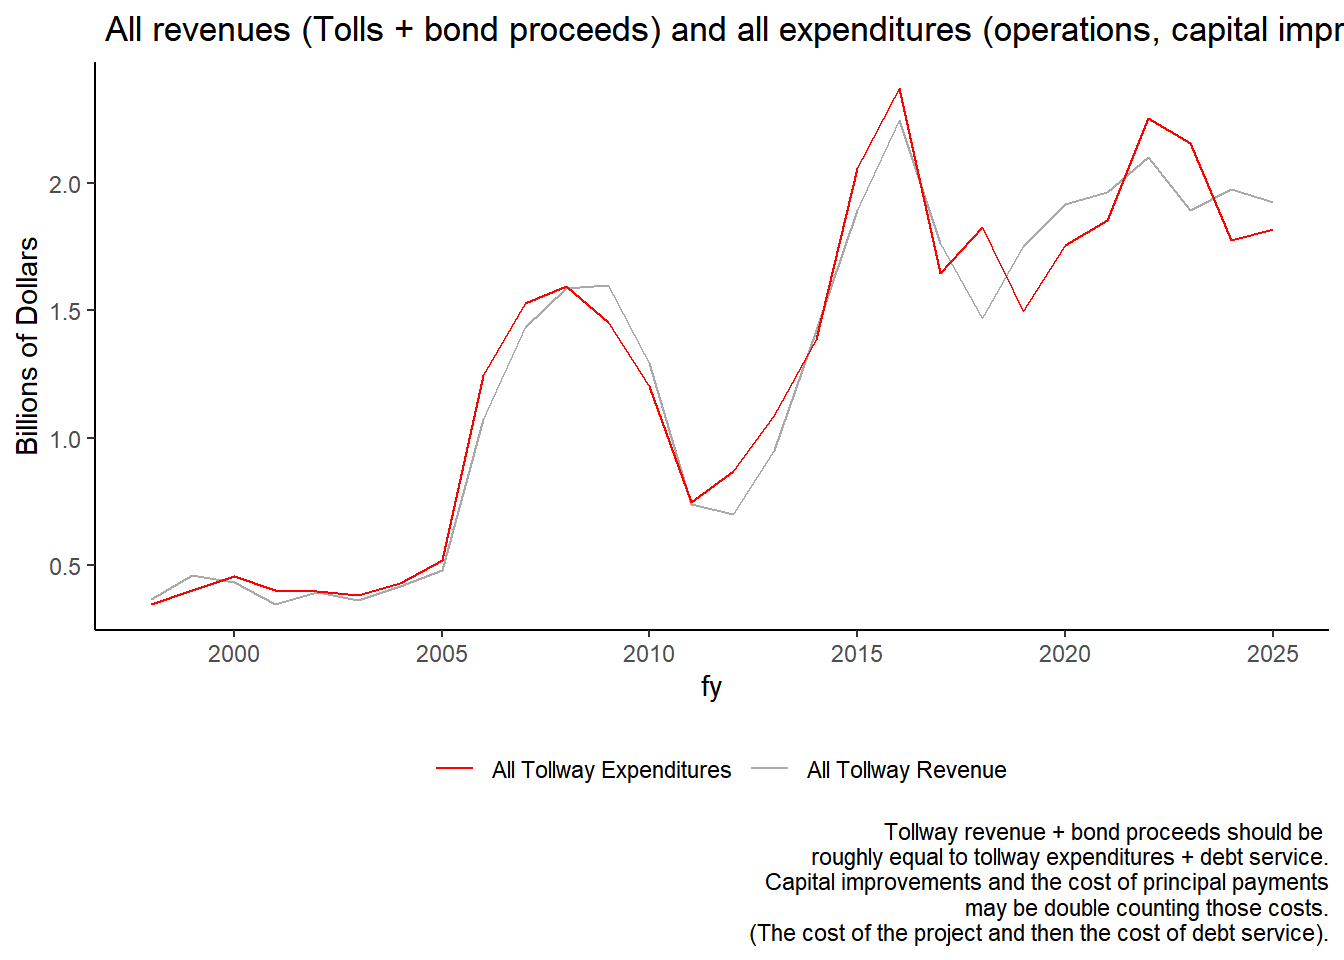
\includegraphics{./Debt_files/figure-pdf/tollway-2.pdf}

}

\end{figure}

\hypertarget{section-2}{%
\subsubsection{}\label{section-2}}

\begin{Shaded}
\begin{Highlighting}[]
\NormalTok{all\_debt }\SpecialCharTok{\%\textgreater{}\%}  \CommentTok{\# all debt does NOT include the tollway expenditures}
  \FunctionTok{ggplot}\NormalTok{() }\SpecialCharTok{+} 
    \FunctionTok{geom\_line}\NormalTok{(}\FunctionTok{aes}\NormalTok{(}\AttributeTok{x=}\NormalTok{fy, }\AttributeTok{y=}\NormalTok{principal}\SpecialCharTok{/}\DecValTok{1000000}\NormalTok{, }\AttributeTok{color =} \StringTok{"Principal"}\NormalTok{))}\SpecialCharTok{+} 
    \FunctionTok{geom\_line}\NormalTok{(}\FunctionTok{aes}\NormalTok{(}\AttributeTok{x=}\NormalTok{fy, }\AttributeTok{y=}\NormalTok{interest}\SpecialCharTok{/}\DecValTok{1000000}\NormalTok{, }\AttributeTok{color =} \StringTok{"Interest"}\NormalTok{))}\SpecialCharTok{+}
    \FunctionTok{geom\_line}\NormalTok{(}\FunctionTok{aes}\NormalTok{(}\AttributeTok{x=}\NormalTok{fy, }\AttributeTok{y =}\NormalTok{ CapitalProjects }\SpecialCharTok{/} \DecValTok{1000000}\NormalTok{, }\AttributeTok{color =} \StringTok{"Capital Projects Debt Service"}\NormalTok{))}\SpecialCharTok{+}
    \FunctionTok{geom\_line}\NormalTok{(}\AttributeTok{data =}\NormalTok{ tollwaydebt, }\FunctionTok{aes}\NormalTok{( }\AttributeTok{x=}\NormalTok{fy, }\AttributeTok{y=}\NormalTok{sum}\SpecialCharTok{/}\DecValTok{1000000}\NormalTok{, }\AttributeTok{color =} \StringTok{"Tollway Debt Service"}\NormalTok{))}\SpecialCharTok{+}
  \FunctionTok{theme}\NormalTok{(}\AttributeTok{legend.position =} \StringTok{"bottom"}\NormalTok{) }\SpecialCharTok{+}
    \FunctionTok{labs}\NormalTok{(}\AttributeTok{y =} \StringTok{"Debt ($Millions)"}\NormalTok{, }\AttributeTok{title =} \StringTok{"Short term borrowing and GO Bonds"}\NormalTok{,}
         \AttributeTok{subtitle =} \StringTok{"Principal and Interest payments"}\NormalTok{, }
         \AttributeTok{caption =} \StringTok{"Capital projects (object 8800) does not include Illinois tollway debt service (fund 0455).}
\StringTok{         Tollway debt service is graphed separately.}
\StringTok{         "}\NormalTok{) }
\end{Highlighting}
\end{Shaded}

\begin{figure}[H]

{\centering 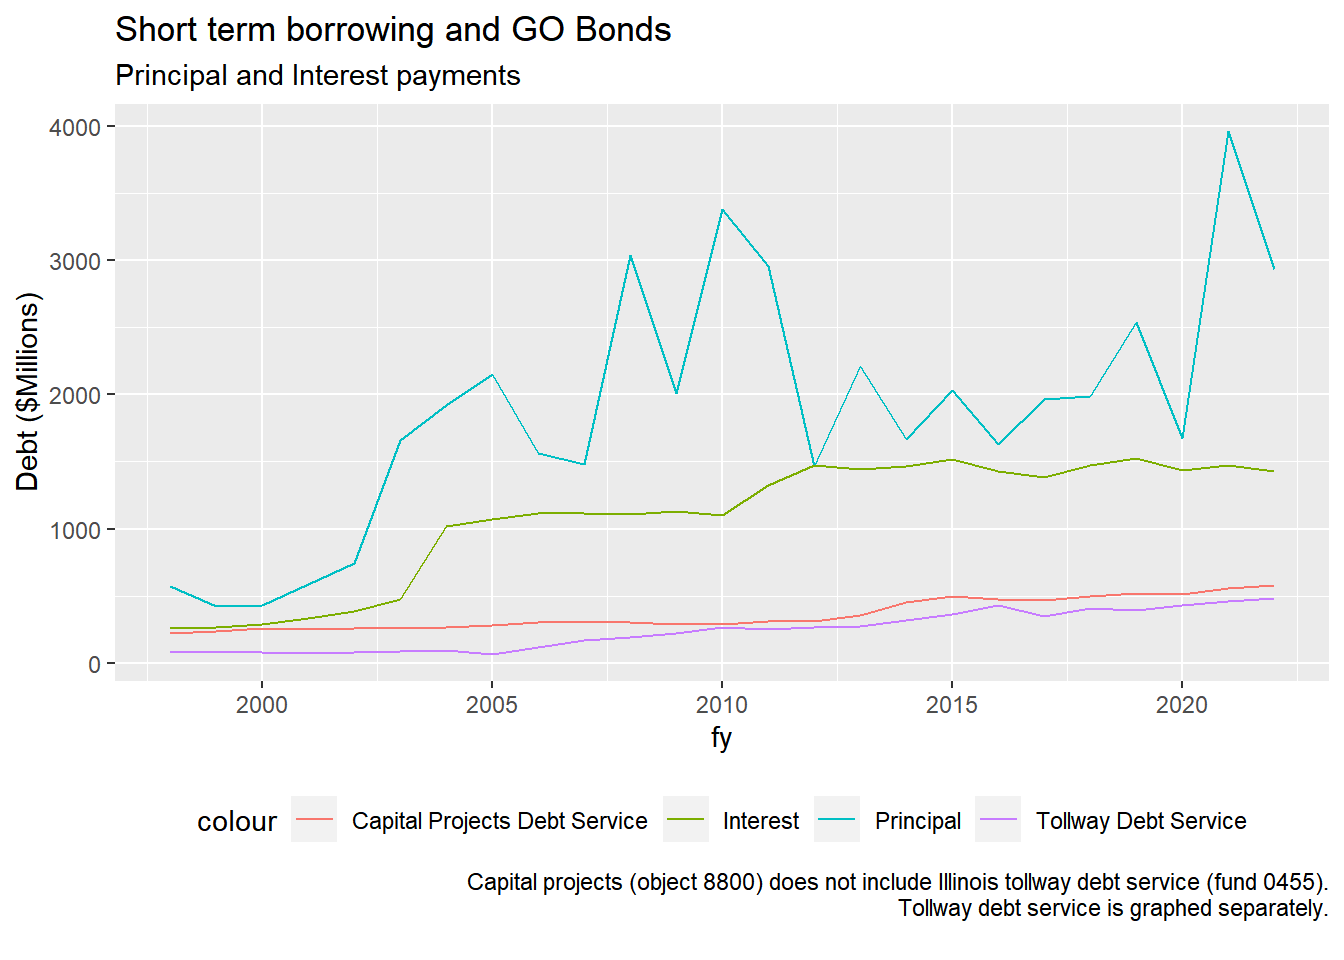
\includegraphics{./Debt_files/figure-pdf/unnamed-chunk-6-1.pdf}

}

\end{figure}

\begin{Shaded}
\begin{Highlighting}[]
\NormalTok{all\_debt }\SpecialCharTok{\%\textgreater{}\%} 
  \FunctionTok{ggplot}\NormalTok{() }\SpecialCharTok{+} 
    \FunctionTok{geom\_line}\NormalTok{(}\FunctionTok{aes}\NormalTok{(}\AttributeTok{x=}\NormalTok{fy, }\AttributeTok{y=}\NormalTok{(principal}\SpecialCharTok{+}\NormalTok{interest}\SpecialCharTok{+}\NormalTok{CapitalProjects)}\SpecialCharTok{/}\DecValTok{1000000}\NormalTok{, }\AttributeTok{color =} \StringTok{"All Principal \& Interest"}\NormalTok{))}\SpecialCharTok{+} 
    \CommentTok{\#geom\_line(aes(x=fy, y=interest/1000000, color = "Interest"))+}
  \CommentTok{\#  geom\_line(aes(x=fy, y = CapitalProjects / 1000000, color = "Capital Projects Debt Service"))+}
    \FunctionTok{geom\_line}\NormalTok{(}\AttributeTok{data =}\NormalTok{ tollwaydebt, }\FunctionTok{aes}\NormalTok{( }\AttributeTok{x=}\NormalTok{fy, }\AttributeTok{y=}\NormalTok{sum}\SpecialCharTok{/}\DecValTok{1000000}\NormalTok{, }\AttributeTok{color =} \StringTok{"Tollway Debt Service"}\NormalTok{))}\SpecialCharTok{+}
    \FunctionTok{theme}\NormalTok{(}\AttributeTok{legend.position =} \StringTok{"bottom"}\NormalTok{) }\SpecialCharTok{+}
    \FunctionTok{labs}\NormalTok{(}\AttributeTok{y =} \StringTok{"Debt ($Millions)"}\NormalTok{, }\AttributeTok{title =} \StringTok{"Illinois Debt Service Expenditure"}\NormalTok{,}
         \AttributeTok{subtitle =} \StringTok{"All Principal and Interest payments"}\NormalTok{, }\AttributeTok{caption =} \StringTok{"All principal and interest includes short{-}term borrowing, GO bonds, and capital projects debt service }
\StringTok{         EXCEPT the Illinois Tollway debt service. Illinois tollway debt service is graphed separately."}\NormalTok{) }
\end{Highlighting}
\end{Shaded}

\begin{figure}[H]

{\centering 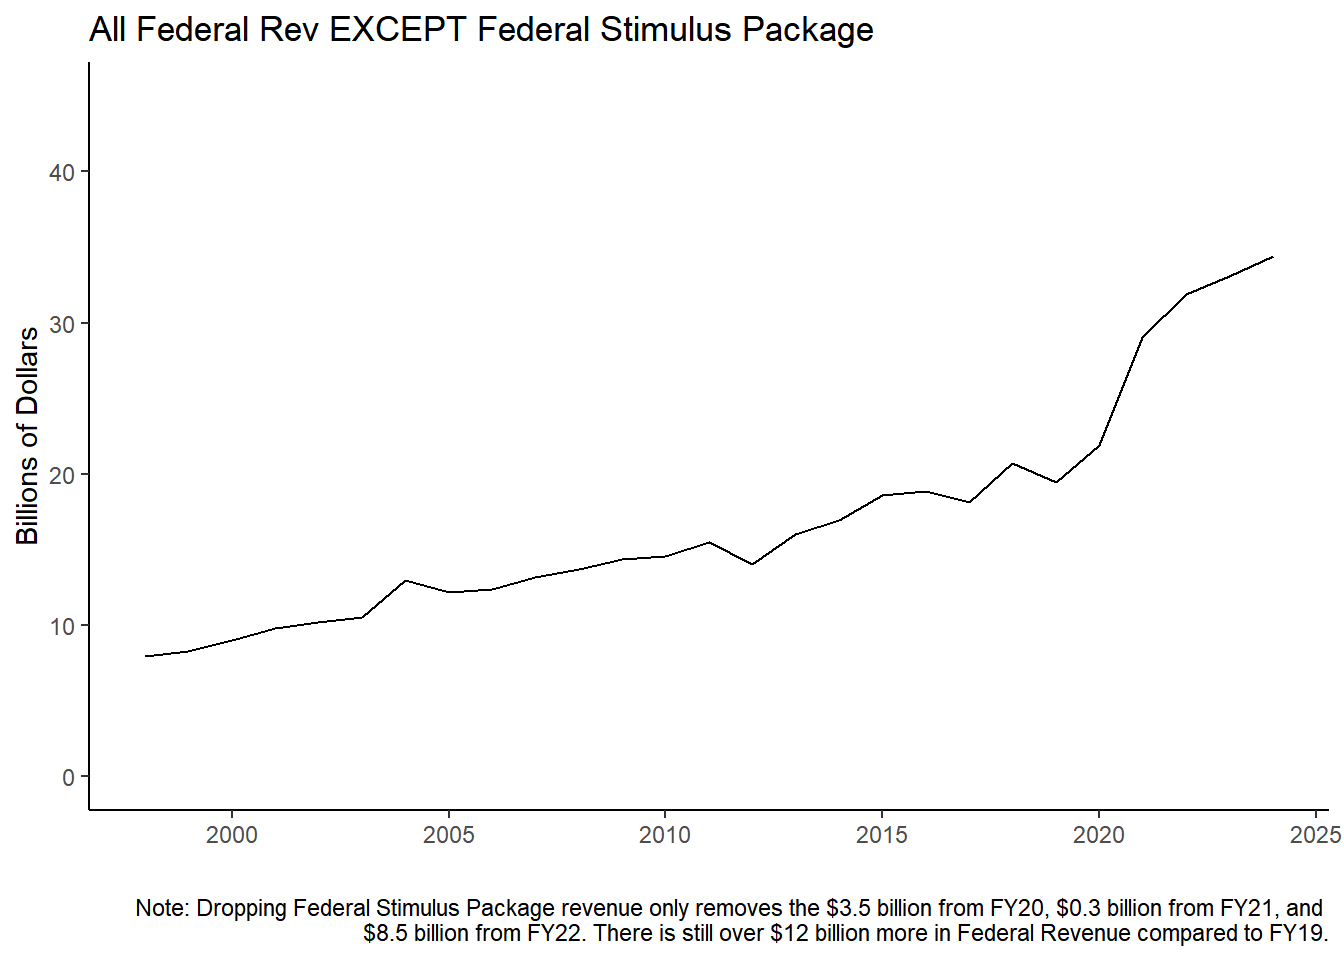
\includegraphics{./Debt_files/figure-pdf/unnamed-chunk-6-2.pdf}

}

\end{figure}

\bookmarksetup{startatroot}

\hypertarget{pensions}{%
\chapter{Pensions}\label{pensions}}

\begin{Shaded}
\begin{Highlighting}[]
\FunctionTok{library}\NormalTok{(tidyverse)}
\FunctionTok{library}\NormalTok{(haven)}
\FunctionTok{library}\NormalTok{(formatR)}
\FunctionTok{library}\NormalTok{(lubridate)}
\FunctionTok{library}\NormalTok{(smooth)}
\FunctionTok{library}\NormalTok{(scales)}
\FunctionTok{library}\NormalTok{(kableExtra)}
\FunctionTok{library}\NormalTok{(ggplot2)}
\FunctionTok{library}\NormalTok{(readxl)}
\FunctionTok{library}\NormalTok{(tidyverse)}
\FunctionTok{library}\NormalTok{(data.table)}
\FunctionTok{library}\NormalTok{(janitor)}


\NormalTok{knitr}\SpecialCharTok{::}\NormalTok{opts\_chunk}\SpecialCharTok{$}\FunctionTok{set}\NormalTok{(}\AttributeTok{echo =} \ConstantTok{TRUE}\NormalTok{, }\AttributeTok{warning =} \ConstantTok{FALSE}\NormalTok{, }\AttributeTok{message =} \ConstantTok{FALSE}\NormalTok{)}
\end{Highlighting}
\end{Shaded}

\textbf{For yearly expenditure calculations, the state contributions to
the pension funds (object = 4431) should be the expenditure included for
pensions. If trying to look at the bigger fiscal health picture and
include unfunded liabilities and in/out flows, then items like purchase
of investments and POB spikes in trends that occurred from policy
changes should be analyzed and discussed in a separate section. Again,
State contributions TO the pension funds are the expenditures BUT an
additional graph/discussion on the employer contributions, employee
contributions, and benefits paid out should be included and considered
for additional context on Illinois' situation.}

Pension expenditures referenced in the analysis are based on state
payments to the following pension systems:

\begin{itemize}
\tightlist
\item
  Teachers Retirement System (TRS)
\item
  New POB bond in 2019: Accelerated Bond Fund paid benefits in advance
  as lump sum
\item
  State Employee Retirement System (SERS)
\item
  State University Retirement System (SURS)
\item
  Judges Retirement System (JRS)
\item
  General Assembly Retirement System (GARS)
\end{itemize}

Employer contributions for pensions are excluded from analysis to avoid
double counting the cost of pensions. Expenditures with object 4430 for
pensions, benefits, and annuities appears in items from funds 0473,
0477, 0479, 0481, (TRS, JRS, SERS, GARS), 0755, 0786, 0787, 0788, 0789,
0799 (deferred compensation plan, GAR excess benefit, JRS excess
benefit, SER excess benefit, TRS excess benefit, state university
retirement system) are NOT included in the analysis. All are coded with
in\_ff=0 in the fund\_ab\_in.xlsx file of funds.

Most of these funds were found by either using CTRL-F with pension
related words or scrolling through code options on the comptroller's
website.

\begin{Shaded}
\begin{Highlighting}[]
\NormalTok{exp\_temp }\OtherTok{\textless{}{-}} \FunctionTok{read\_csv}\NormalTok{(}\StringTok{"exp\_temp.csv"}\NormalTok{) }\SpecialCharTok{\%\textgreater{}\%} \FunctionTok{filter}\NormalTok{(agency }\SpecialCharTok{!=} \StringTok{"799"}\NormalTok{)}
\NormalTok{rev\_temp }\OtherTok{\textless{}{-}} \FunctionTok{read\_csv}\NormalTok{(}\StringTok{"rev\_temp.csv"}\NormalTok{) }\SpecialCharTok{\%\textgreater{}\%} \FunctionTok{filter}\NormalTok{(agency}\SpecialCharTok{!=} \StringTok{"799"}\NormalTok{)}


\CommentTok{\# check what is being included in pensions}

\CommentTok{\# funds related to pension contributions}
\NormalTok{pension\_funds }\OtherTok{\textless{}{-}} \FunctionTok{c}\NormalTok{(}\StringTok{"0472"}\NormalTok{, }\StringTok{"0473"}\NormalTok{, }\StringTok{"0477"}\NormalTok{, }\StringTok{"0479"}\NormalTok{, }\StringTok{"0481"}\NormalTok{, }\StringTok{"0755"}\NormalTok{, }\StringTok{"0786"}\NormalTok{, }\StringTok{"0787"}\NormalTok{, }\StringTok{"0788"}\NormalTok{, }\StringTok{"0789"}\NormalTok{, }\StringTok{"0799"}\NormalTok{)}

\NormalTok{pension\_check }\OtherTok{\textless{}{-}}\NormalTok{ exp\_temp }\SpecialCharTok{\%\textgreater{}\%} 
  \FunctionTok{mutate}\NormalTok{(}\AttributeTok{pension =} \FunctionTok{case\_when}\NormalTok{( }
 \CommentTok{\# object == "4430" \& fund == "0825" \textasciitilde{} "Object 4430 {-} Pension Buyout/Benefits Paid Early",}
\NormalTok{    (object}\SpecialCharTok{==}\StringTok{"4430"}\NormalTok{) }\SpecialCharTok{\textasciitilde{}} \StringTok{"Object 4430 {-} Benefits Paid to Employees; EXCLUDED"}\NormalTok{, }\CommentTok{\# pensions, annuities, benefits}
\NormalTok{    (object}\SpecialCharTok{==}\StringTok{"4431"}\NormalTok{) }\SpecialCharTok{\textasciitilde{}} \StringTok{"Object 4431 {-} State Contributions; INCLUDED"}\NormalTok{, }\CommentTok{\# 4431 = state payments into pension fund}
\NormalTok{        (obj\_seq\_type }\SpecialCharTok{\textgreater{}} \StringTok{"11590000"} \SpecialCharTok{\&}\NormalTok{ obj\_seq\_type }\SpecialCharTok{\textless{}} \StringTok{"11660000"}\NormalTok{)  }\SpecialCharTok{\textasciitilde{}} \StringTok{"Object 1160{-}1165 Employer Contributions to Pension Fund; EXCLUDED"}\NormalTok{,}
    \CommentTok{\# objects 1159 to 1166 are all considered Retirement by Comptroller }
    
            \ConstantTok{TRUE} \SpecialCharTok{\textasciitilde{}} \StringTok{"0"}\NormalTok{)) }\SpecialCharTok{\%\textgreater{}\%}  \CommentTok{\# All other observations coded as 0 for non{-}pension items}
  
  \CommentTok{\# recodes specific instances of code anomalies from past years:}
  \FunctionTok{mutate}\NormalTok{(}\AttributeTok{pension =} \FunctionTok{case\_when}\NormalTok{(}
\NormalTok{    (object}\SpecialCharTok{==}\StringTok{"1298"} \SpecialCharTok{\&}\NormalTok{ fund }\SpecialCharTok{\%in\%}\NormalTok{ pension\_funds ) }\SpecialCharTok{\textasciitilde{}} \StringTok{"Object 1298 {-} Purchase of Investments; DROPPED"}\NormalTok{, }

    
      \CommentTok{\# pension stabilization fund in 2022 }
 \CommentTok{\# object == "1900" \& fund == "0319" \textasciitilde{} "Fund 0319{-}Pension Stabilization", }
\NormalTok{    object }\SpecialCharTok{==} \StringTok{"1900"} \SpecialCharTok{\&}\NormalTok{ fund }\SpecialCharTok{\%in\%}\NormalTok{ pension\_funds }\SpecialCharTok{\textasciitilde{}} \StringTok{"Fund 0319 {-} Pension Stabilization"}\NormalTok{, }

  
\NormalTok{  object }\SpecialCharTok{==} \StringTok{"4900"} \SpecialCharTok{\&}\NormalTok{ fund }\SpecialCharTok{\%in\%}\NormalTok{ pension\_funds }\SpecialCharTok{\textasciitilde{}} \StringTok{"Object 4900 {-} Awards/Grants; Weird 2010{-}2011 values"}\NormalTok{,}
  
    \ConstantTok{TRUE} \SpecialCharTok{\textasciitilde{}} \FunctionTok{as.character}\NormalTok{(pension)) ) }\SpecialCharTok{\%\textgreater{}\%} 
  \FunctionTok{filter}\NormalTok{(pension }\SpecialCharTok{!=} \StringTok{"0"}\NormalTok{ )}

\NormalTok{pension\_check }\SpecialCharTok{\%\textgreater{}\%} \FunctionTok{group\_by}\NormalTok{(fy, pension) }\SpecialCharTok{\%\textgreater{}\%} 
  \FunctionTok{summarize}\NormalTok{(}\AttributeTok{expenditure =} \FunctionTok{sum}\NormalTok{(expenditure, }\AttributeTok{na.rm =} \ConstantTok{TRUE}\NormalTok{)) }\SpecialCharTok{\%\textgreater{}\%}
  \FunctionTok{ggplot}\NormalTok{(}\FunctionTok{aes}\NormalTok{(}\AttributeTok{x=}\NormalTok{fy, }\AttributeTok{y =}\NormalTok{ expenditure}\SpecialCharTok{/}\DecValTok{1000000000}\NormalTok{, }\AttributeTok{color =}\NormalTok{ pension)) }\SpecialCharTok{+} 
  \FunctionTok{geom\_line}\NormalTok{() }\SpecialCharTok{+} 

  \FunctionTok{labs}\NormalTok{ (}\AttributeTok{title =} \StringTok{"Pension Fund Payments In and Retirement Benefits Out"}\NormalTok{, }
  \AttributeTok{caption =} \StringTok{"Object 4430 is retirement benefits paid to employees. }
\StringTok{  Object 4431 includes state payments INTO pension Fund.}
\StringTok{  Object 1298 is excluded except for years 2010 and 2011 due to POBs."}\NormalTok{,}
  \AttributeTok{y=} \StringTok{"Billions of Dollars"}\NormalTok{)}\SpecialCharTok{+}
    \FunctionTok{theme}\NormalTok{(}\AttributeTok{legend.position =} \StringTok{"bottom"}\NormalTok{)}\SpecialCharTok{+}
  \FunctionTok{guides}\NormalTok{(}\AttributeTok{color =} \FunctionTok{guide\_legend}\NormalTok{(}\AttributeTok{nrow=}\DecValTok{3}\NormalTok{))}
\end{Highlighting}
\end{Shaded}

\begin{figure}[H]

{\centering \includegraphics{./Pensions_files/figure-pdf/unnamed-chunk-2-1.pdf}

}

\end{figure}

Pension contributions from employees and employers are not included as
revenue sources but are useful for understanding the money going into
the funds and the money flowing out of the funds. Identifying and
graphing employee and employer contributions, as well as benefits paid
to retired employees and state contributions was important for checking
the items that should and should not be included in the analysis.

\hfill\break

\begin{Shaded}
\begin{Highlighting}[]
\CommentTok{\# rev\_type = 51 is for retirement/pension contributions from both employers and employees.}

\CommentTok{\# current year employee revenue source = 0573, contributions by employee == 572 (stops at 2011)}

\DocumentationTok{\#\# revenue side: \#\#}
\NormalTok{retirement\_contributions }\OtherTok{\textless{}{-}}\NormalTok{ rev\_temp }\SpecialCharTok{\%\textgreater{}\%} 
  \FunctionTok{filter}\NormalTok{(rev\_type }\SpecialCharTok{==} \StringTok{"51"}\NormalTok{) }\SpecialCharTok{\%\textgreater{}\%} \FunctionTok{group\_by}\NormalTok{(fy) }\SpecialCharTok{\%\textgreater{}\%} \FunctionTok{summarize}\NormalTok{(}\AttributeTok{contributions =} \FunctionTok{sum}\NormalTok{(receipts))}

\NormalTok{employer\_contributions }\OtherTok{\textless{}{-}}\NormalTok{ rev\_temp }\SpecialCharTok{\%\textgreater{}\%} 
  \FunctionTok{filter}\NormalTok{(rev\_type }\SpecialCharTok{==} \StringTok{"51"} \SpecialCharTok{\&}\NormalTok{ source }\SpecialCharTok{==} \StringTok{"0577"}\NormalTok{) }\SpecialCharTok{\%\textgreater{}\%} \FunctionTok{group\_by}\NormalTok{(fy) }\SpecialCharTok{\%\textgreater{}\%} \FunctionTok{summarize}\NormalTok{(}\AttributeTok{contributions =} \FunctionTok{sum}\NormalTok{(receipts))}

\NormalTok{employee\_contributions }\OtherTok{\textless{}{-}}\NormalTok{ rev\_temp }\SpecialCharTok{\%\textgreater{}\%} 
  \FunctionTok{filter}\NormalTok{(rev\_type }\SpecialCharTok{==} \StringTok{"51"} \SpecialCharTok{\&}\NormalTok{ (source }\SpecialCharTok{==} \StringTok{"0572"} \SpecialCharTok{|}\NormalTok{ source }\SpecialCharTok{==} \StringTok{"0573"}\NormalTok{) ) }\SpecialCharTok{\%\textgreater{}\%} 
  \FunctionTok{group\_by}\NormalTok{(fy) }\SpecialCharTok{\%\textgreater{}\%} \FunctionTok{summarize}\NormalTok{(}\AttributeTok{contributions =} \FunctionTok{sum}\NormalTok{(receipts))}


\DocumentationTok{\#\# expenditure side }\AlertTok{\#\#\#}\DocumentationTok{ }
\NormalTok{benefits\_paid }\OtherTok{\textless{}{-}}\NormalTok{ pension\_check }\SpecialCharTok{\%\textgreater{}\%} \FunctionTok{filter}\NormalTok{(object }\SpecialCharTok{==} \StringTok{"4430"}\NormalTok{) }\SpecialCharTok{\%\textgreater{}\%}
  \FunctionTok{group\_by}\NormalTok{(fy) }\SpecialCharTok{\%\textgreater{}\%} 
  \FunctionTok{summarize}\NormalTok{(}\AttributeTok{expenditure =} \FunctionTok{sum}\NormalTok{(expenditure, }\AttributeTok{na.rm =} \ConstantTok{TRUE}\NormalTok{))}

\NormalTok{state\_contrib }\OtherTok{\textless{}{-}}\NormalTok{ pension\_check }\SpecialCharTok{\%\textgreater{}\%} \FunctionTok{filter}\NormalTok{(object }\SpecialCharTok{==} \StringTok{"4431"}\NormalTok{) }\SpecialCharTok{\%\textgreater{}\%}
  \FunctionTok{group\_by}\NormalTok{(fy) }\SpecialCharTok{\%\textgreater{}\%} 
  \FunctionTok{summarize}\NormalTok{(}\AttributeTok{expenditure =} \FunctionTok{sum}\NormalTok{(expenditure, }\AttributeTok{na.rm =} \ConstantTok{TRUE}\NormalTok{))}



\NormalTok{rev\_temp }\SpecialCharTok{\%\textgreater{}\%} 
  \FunctionTok{filter}\NormalTok{(rev\_type }\SpecialCharTok{==} \StringTok{"51"}\NormalTok{) }\SpecialCharTok{\%\textgreater{}\%} \CommentTok{\# all retirement contributions}
  \FunctionTok{group\_by}\NormalTok{(fy, source) }\SpecialCharTok{\%\textgreater{}\%} 
  \FunctionTok{summarise}\NormalTok{(}\AttributeTok{sum =} \FunctionTok{sum}\NormalTok{(receipts, }\AttributeTok{na.rm =} \ConstantTok{TRUE}\NormalTok{)) }\SpecialCharTok{\%\textgreater{}\%}
  \FunctionTok{ggplot}\NormalTok{() }\SpecialCharTok{+}
  \FunctionTok{geom\_line}\NormalTok{(}\FunctionTok{aes}\NormalTok{(}\AttributeTok{x=}\NormalTok{fy, }\AttributeTok{y =}\NormalTok{ sum, }\AttributeTok{color=}\NormalTok{source)) }\SpecialCharTok{+} \FunctionTok{labs}\NormalTok{(}\AttributeTok{title=}\StringTok{"Retirement Contribution Sources, ALL rev\_source == 51"}\NormalTok{, }
       \AttributeTok{caption =} \StringTok{"Source 0573, 0572 is for employee contributions. 0577 is Contributions by employer."}\NormalTok{)}
\end{Highlighting}
\end{Shaded}

\begin{figure}[H]

{\centering \includegraphics{./Pensions_files/figure-pdf/unnamed-chunk-3-1.pdf}

}

\end{figure}

\textbf{Additional pension info:}\\
For the \$10 billion in 2004, they borrowed money and invested it in
pension portfolio and hoped that the returns would be greater than the
interest on the debt. If returns\textgreater interest, then they
increased the pension funds and it was a good idea. Otherwise a short
term band-aid causes even more problems later. This added a significant
amount to the unfunded pension liabilities. In 2010 and 2011, POBs
served as a type of general borrowing for the state by borrowing against
what was owed to the pension systems and using that revenue that should
have funded pensions to instead subsidize the cost of providing core
services. Illinois borrowed money (POBs) and used it to pay for
government services. A temporary way to fill a budget gap for that 2010
that then costs more in the long run due to increased unfunded
liabilities and interest on the borrowed money. - ``Basket Case'' by Dye
2015 but summarized much more casually by Alea WM

In 2019 lawmakers offered a pension buyout plan where members could
opt-out of their future benefits for a lump sum. However, few people
participated in the buyout plan and very little savings have occurred so
far. The buyout plan has been extended to 2026 in hopes that more people
participate in it. Description of Pension Obligation Acceleration Bond
at this
\href{https://www.ilga.gov/legislation/ilcs/documents/003003300K7.7.htm}{link}.
Proceeds of bonds go into pension obligation acceleration fund (which
are not included as a revenue source) and the fund is only used to make
accelerated pension benefit payments. The pension stabilization fund
(0319) is money put into the pension funds to help pay for unfunded
liabilities from past poor budgeting decisions.

\hypertarget{data-coding-details}{%
\subsection{\texorpdfstring{\textbf{Data coding
details}}{Data coding details}}\label{data-coding-details}}

\begin{itemize}
\tightlist
\item
  State pension contributions are largely captured with object=4431.
  \textbf{(These are the State expenditures included in analysis)}

  \begin{itemize}
  \tightlist
  \item
    includes 8 billion payment in 2004 that creates large peak in
    expenditure graph
  \item
    Object 4431 does not capture recent pension stabilization fund which
    is fund = 0319, object = 1900 and has \$300 million investment in
    FY2022.
  \end{itemize}
\item
  Fund=0475 is the Municipal Retirement Fund - Not included because
  state just helps collect and disperse local pension funds. IMRF is
  most funded pension fund in Illinois. Fund ends in 2015. All were
  considered purchase of investments.
\item
  IOC objects 1160-1165 are for all retirement expenditures for
  employers. These are not included in the analysis as pension costs.

  \begin{itemize}
  \tightlist
  \item
    object = 1167 and 1168 is for Employer pension contributions but is
    not used by IOC yet as of FY2022
  \end{itemize}
\item
  Some expenditures with object=4430 (benefits paid to retirees) were
  paid for with Pension obligation bond funds (fund == 0825).
\item
  In past years, some POB funded expenditures were moved to revenue
  side. Code logic was unclear. We are no longer doing this as of
  FY2021.
\item
  Other types of pension expenditures to consider when looking at
  pension funds: Pension obligation acceleration bond, state pension
  obligation bond reimbursements, pension pickup, accelerated pension
  buy-out (bond financed funds)
\item
  object = 1298 is for Purchase of Investments and is excluded from
  analysis. In past analyses, there were a couple of exceptions during
  2010 and 2011.

  \begin{itemize}
  \tightlist
  \item
    Purchase of Investments captures the pension obligation bonds issued
    in 2010-2011.
  \end{itemize}
\item
  object = 1900 for pension stabilization is under lump sums
\item
  object = 4900 is awards and grants lump sum
\end{itemize}

\bookmarksetup{startatroot}

\hypertarget{state-employee-healthcare-discussion}{%
\chapter{State Employee Healthcare
Discussion}\label{state-employee-healthcare-discussion}}

State Employee Health Care = Sum of expenditures for ``health care
coverage as elected by members per state employees group insurance
act.'' The payments are made from the Health Insurance Reserve Fund.
Employee contributions are not considered a revenue source or an
expenditure in our analysis.

Funding for the State Employees Group Insurance plan originates from two
funds. The Health Insurance Reserve Fund (HIRF) and the Group Insurance
Premium Fund (GIPF). Contributions and payment for Health coverage
benefits are deposited INTO HIRF and contributions for life insurance
are deposited into the GIPF.

HIRF is the fund mainly used to administer the group insurance program.
Funding for HIRF comes from several different revenue sources: the
General Revenue Fund (GRF), Road Fund, reimbursements, university funds,
and misc funds. Source:
\href{https://cgfa.ilga.gov/Upload/fy2011stateemployees\textquotesingle{}groupinsurance.pdf}{CGFA
Report}.

\hypertarget{coding-details-1}{%
\subsection{\texorpdfstring{\textbf{Coding
details}}{Coding details}}\label{coding-details-1}}

In FY2013, the Local Government Health Insurance fund was transferred to
the department of Central Management Services (agency changes from 478
to 416 in data.)

Employer group insurance contributions for health insurance are excluded
to avoid double counting the cost of healthcare provision. All employer
group insurance contributions are coded as object = 1180. BUT the last
two fiscal years (FY21 and FY22) were coded as 1900 instead of 1180 for
lump sums instead of employer contributions. This caused an
\textasciitilde\$2 billion miscalculation when writing the FY21 paper
that was caught before publishing.

\begin{itemize}
\tightlist
\item
  Fund = 0907 = Health Insurance Reserve Fund, in\_ff = 1
\item
  Fund = 0457 is ``Group Insurance Premium Fund'', in\_ff = 1
\item
  Fund = 0193 is ``Local govt health insurance reserve'', in=ff = 0
\item
  fund = 0477 is ``Community College Health Insurance'', in=ff = 0.

  \begin{itemize}
  \tightlist
  \item
    had large amount in early years
  \end{itemize}
\item
  Fund = 9939 is ``group self-insurers' insolv'', in\_ff = 1
\item
  Fund = 0940 is Self-Insurers security, in\_ff = 0
\item
  Fund = 0739 is Group Workers Comp Pool Insol, in\_ff = 1

  \begin{itemize}
  \item
    eehc = 0 means it is NOT a state healthcare cost but it is an
    employer contribution of some type to some fund
  \item
    eehc = 1 means it is a state employee healthcare cost and it is an
    employer contribution to health insurance
  \end{itemize}
\end{itemize}

If observation is a group insurance contribution, then the expenditure
amount is set to \$0 (essentially dropped from analysis).

\begin{Shaded}
\begin{Highlighting}[]
\NormalTok{exp\_temp }\OtherTok{\textless{}{-}} \FunctionTok{read\_csv}\NormalTok{(}\StringTok{"exp\_temp.csv"}\NormalTok{)}
\NormalTok{rev\_temp }\OtherTok{\textless{}{-}} \FunctionTok{read\_csv}\NormalTok{(}\StringTok{"rev\_temp.csv"}\NormalTok{)}


\NormalTok{health\_ins\_reserve }\OtherTok{\textless{}{-}}\NormalTok{ exp\_temp }\SpecialCharTok{\%\textgreater{}\%} 
  \FunctionTok{filter}\NormalTok{(fund }\SpecialCharTok{==} \StringTok{"0907"}\NormalTok{) }\SpecialCharTok{\%\textgreater{}\%}  
  \FunctionTok{group\_by}\NormalTok{(fy) }\SpecialCharTok{\%\textgreater{}\%} 
  \FunctionTok{summarize}\NormalTok{(}\AttributeTok{fund\_0907 =} \FunctionTok{sum}\NormalTok{(expenditure)) }

\NormalTok{health\_ins\_reserve }\SpecialCharTok{\%\textgreater{}\%} 
  \FunctionTok{ggplot}\NormalTok{(}\FunctionTok{aes}\NormalTok{(}\AttributeTok{x=}\NormalTok{fy, }\AttributeTok{y=}\NormalTok{fund\_0907)) }\SpecialCharTok{+} 
  \FunctionTok{geom\_col}\NormalTok{() }\SpecialCharTok{+} 
  \FunctionTok{labs}\NormalTok{(}\AttributeTok{title=}\StringTok{"Health Insurance Reserve"}\NormalTok{, }\AttributeTok{subtitle =} \StringTok{"Sum of expenditures from fund 907"}\NormalTok{)}
\end{Highlighting}
\end{Shaded}

\begin{figure}[H]

{\centering \includegraphics{./Healthcare_files/figure-pdf/healthcare-employer-contributions-1.pdf}

}

\end{figure}

\begin{Shaded}
\begin{Highlighting}[]
\CommentTok{\# object 1180 is inconsistently coded over time form the IOC }

\CommentTok{\# object 1180 should be employer contributions to healthcare group insurance}

\NormalTok{employer\_contributions }\OtherTok{\textless{}{-}}\NormalTok{ exp\_temp }\SpecialCharTok{\%\textgreater{}\%} 
  \FunctionTok{filter}\NormalTok{(object }\SpecialCharTok{==} \StringTok{"1180"}\NormalTok{) }\SpecialCharTok{\%\textgreater{}\%} 
  \FunctionTok{group\_by}\NormalTok{(fy) }\SpecialCharTok{\%\textgreater{}\%} 
  \FunctionTok{summarize}\NormalTok{(}\AttributeTok{object1180 =} \FunctionTok{sum}\NormalTok{(expenditure)) }

\NormalTok{employer\_contributions}\SpecialCharTok{\%\textgreater{}\%} 
  \FunctionTok{ggplot}\NormalTok{(}\FunctionTok{aes}\NormalTok{(}\AttributeTok{x=}\NormalTok{fy, }\AttributeTok{y=}\NormalTok{object1180)) }\SpecialCharTok{+} 
  \FunctionTok{geom\_col}\NormalTok{() }\SpecialCharTok{+} 
  \FunctionTok{labs}\NormalTok{(}\AttributeTok{title=}\StringTok{"Employer Contributions to Healthcare Group Insurance, IOC Object 1180"}\NormalTok{)}
\end{Highlighting}
\end{Shaded}

\begin{figure}[H]

{\centering \includegraphics{./Healthcare_files/figure-pdf/healthcare-employer-contributions-2.pdf}

}

\end{figure}

\begin{Shaded}
\begin{Highlighting}[]
\NormalTok{employer\_contributions2 }\OtherTok{\textless{}{-}}\NormalTok{ exp\_temp }\SpecialCharTok{\%\textgreater{}\%} 
  \FunctionTok{filter}\NormalTok{(object }\SpecialCharTok{==} \StringTok{"1180"} \SpecialCharTok{\&}\NormalTok{ fund}\SpecialCharTok{==}\StringTok{"0001"}\NormalTok{) }\SpecialCharTok{\%\textgreater{}\%} 
  \FunctionTok{group\_by}\NormalTok{(fy) }\SpecialCharTok{\%\textgreater{}\%} 
  \FunctionTok{summarize}\NormalTok{(}\AttributeTok{object1180 =} \FunctionTok{sum}\NormalTok{(expenditure)) }

\NormalTok{employer\_contributions2 }\SpecialCharTok{\%\textgreater{}\%} 
  \FunctionTok{ggplot}\NormalTok{(}\FunctionTok{aes}\NormalTok{(}\AttributeTok{x=}\NormalTok{fy, }\AttributeTok{y=}\NormalTok{object1180)) }\SpecialCharTok{+} 
  \FunctionTok{geom\_col}\NormalTok{() }\SpecialCharTok{+} 
  \FunctionTok{labs}\NormalTok{(}\AttributeTok{title=}\StringTok{"Employer Contributions to Healthcare Group Insurance"}\NormalTok{, }
       \AttributeTok{subtitle =} \StringTok{"IOC Object 1180 from Fund 001"}\NormalTok{)}
\end{Highlighting}
\end{Shaded}

\begin{figure}[H]

{\centering \includegraphics{./Healthcare_files/figure-pdf/healthcare-employer-contributions-3.pdf}

}

\end{figure}

\begin{Shaded}
\begin{Highlighting}[]
\CommentTok{\# examine combined group insurance totals per year}

\NormalTok{group\_ins2 }\OtherTok{\textless{}{-}}\NormalTok{ exp\_temp }\SpecialCharTok{\%\textgreater{}\%} 
  \FunctionTok{mutate}\NormalTok{(}\AttributeTok{eehc =} \FunctionTok{ifelse}\NormalTok{(}
    \CommentTok{\# group insurance contributions for 1998{-}2005 and 2013{-}present}
    \CommentTok{\# CMS took over health insurance in 2013}
\NormalTok{   fund }\SpecialCharTok{==} \StringTok{"0001"} \SpecialCharTok{\&}\NormalTok{ (object }\SpecialCharTok{==} \StringTok{"1180"} \SpecialCharTok{|}\NormalTok{ object }\SpecialCharTok{==}\StringTok{"1900"}\NormalTok{) }\SpecialCharTok{\&}\NormalTok{ agency }\SpecialCharTok{==} \StringTok{"416"} \SpecialCharTok{\&}\NormalTok{ appr\_org}\SpecialCharTok{==}\StringTok{"20"}\NormalTok{, }\DecValTok{1}\NormalTok{, }\DecValTok{0}\NormalTok{) )}\SpecialCharTok{\%\textgreater{}\%} 
  \FunctionTok{mutate}\NormalTok{(}\AttributeTok{eehc =} \FunctionTok{ifelse}\NormalTok{(}
    \CommentTok{\# group insurance contributions for 2006{-}2012}
    \CommentTok{\# health insurance was in healthcare and family services, agency 478 for a few years}
\NormalTok{    fund }\SpecialCharTok{==} \StringTok{"0001"} \SpecialCharTok{\&}\NormalTok{ object }\SpecialCharTok{==} \StringTok{"1180"} \SpecialCharTok{\&}\NormalTok{ agency }\SpecialCharTok{==} \StringTok{"478"} \SpecialCharTok{\&}\NormalTok{ appr\_org}\SpecialCharTok{==}\StringTok{"80"}\NormalTok{, }\DecValTok{1}\NormalTok{, eehc) )}\SpecialCharTok{\%\textgreater{}\%}
  \FunctionTok{filter}\NormalTok{(eehc }\SpecialCharTok{==} \DecValTok{1}\NormalTok{) }\SpecialCharTok{\%\textgreater{}\%} 
    \FunctionTok{group\_by}\NormalTok{(fy) }\SpecialCharTok{\%\textgreater{}\%} 
    \FunctionTok{summarize}\NormalTok{(}\AttributeTok{dropped\_group\_premiums =} \FunctionTok{sum}\NormalTok{(expenditure, }\AttributeTok{na.rm=}\ConstantTok{TRUE}\NormalTok{))}

\NormalTok{group\_ins2 }\SpecialCharTok{\%\textgreater{}\%} \FunctionTok{ggplot}\NormalTok{(}\FunctionTok{aes}\NormalTok{(}\AttributeTok{x=}\NormalTok{fy, }\AttributeTok{y=}\NormalTok{dropped\_group\_premiums)) }\SpecialCharTok{+} 
  \FunctionTok{geom\_col}\NormalTok{() }\SpecialCharTok{+} 
  \FunctionTok{labs}\NormalTok{(}\AttributeTok{title=}\StringTok{"Employer Healthcare Group Insurance Contributions"}\NormalTok{, }
       \AttributeTok{subtitle=} \StringTok{" {-} Dropped from analysis to avoid double counting healthcare expenditures"}\NormalTok{, }
       \AttributeTok{caption =} \StringTok{"Objects 1180 and 1900 from fund 0001. See code for additional coding details."}\NormalTok{)}
\end{Highlighting}
\end{Shaded}

\begin{figure}[H]

{\centering \includegraphics{./Healthcare_files/figure-pdf/healthcare-employer-contributions-4.pdf}

}

\end{figure}

\hypertarget{health-insurance-premiums---revenue-side}{%
\subsection{Health Insurance Premiums - Revenue
Side}\label{health-insurance-premiums---revenue-side}}

Employee insurance premiums for healthcare are a revenue source for the
state in the IOC data but are NOT included in the Fiscal Futures
analysis as a revenue or in fiscal gap calculations.

Source \#'s:

\begin{itemize}
\tightlist
\item
  0120 = ins prem-option life
\item
  0120 = ins prem-optional life/univ
\item
  0347 = optional health - HMO
\item
  0348 = optional health - dental
\item
  0349 = optional health - univ/local SI
\item
  0350 = optional health - univ/local
\item
  0351 = optional health - retirement
\item
  0352 = optional health - retirement SI
\item
  0353 = optional health - retire/dental
\item
  0354 = optional health - retirement hmo
\item
  2199-2209 = various HMOs, dental, health plans from Health Insurance
  Reserve (fund)
\end{itemize}

\begin{Shaded}
\begin{Highlighting}[]
\NormalTok{health\_insurance\_fund\_rev}\OtherTok{\textless{}{-}}\NormalTok{ rev\_temp }\SpecialCharTok{\%\textgreater{}\%} 
  \FunctionTok{filter}\NormalTok{(fund}\SpecialCharTok{==}\StringTok{"0907"}\NormalTok{) }\SpecialCharTok{\%\textgreater{}\%} \CommentTok{\# everything that goes to fund 0907}
    \FunctionTok{group\_by}\NormalTok{(fy) }\SpecialCharTok{\%\textgreater{}\%}
  \FunctionTok{summarize}\NormalTok{(}\AttributeTok{health\_ins\_rev =} \FunctionTok{sum}\NormalTok{(receipts)) }


\NormalTok{health\_insurance\_fund\_rev }\SpecialCharTok{\%\textgreater{}\%} 
  \FunctionTok{ggplot}\NormalTok{(}\FunctionTok{aes}\NormalTok{(}\AttributeTok{x=}\NormalTok{fy, }\AttributeTok{y =}\NormalTok{ health\_ins\_rev)) }\SpecialCharTok{+} 
  \FunctionTok{geom\_col}\NormalTok{() }\SpecialCharTok{+} \FunctionTok{labs}\NormalTok{( }\AttributeTok{title =} \StringTok{"Health insurance fund {-} All revenue, Fund 0907"}\NormalTok{)}
\end{Highlighting}
\end{Shaded}

\begin{figure}[H]

{\centering \includegraphics{./Healthcare_files/figure-pdf/employee-insurance-premiums-1.pdf}

}

\end{figure}

\begin{Shaded}
\begin{Highlighting}[]
\CommentTok{\#Old Stata step: collect optional insurance premiums to fund 0907 for use in eehc expenditure  }
\NormalTok{employee\_health\_premiums }\OtherTok{\textless{}{-}}\NormalTok{ rev\_temp }\SpecialCharTok{\%\textgreater{}\%} 
  \FunctionTok{mutate}\NormalTok{(}\AttributeTok{employee\_premiums =} \FunctionTok{ifelse}\NormalTok{(}
\NormalTok{    fund}\SpecialCharTok{==}\StringTok{"0907"} \SpecialCharTok{\&}\NormalTok{ (source}\SpecialCharTok{==}\StringTok{"0120"}\SpecialCharTok{|}\NormalTok{ source}\SpecialCharTok{==}\StringTok{"0121"}\SpecialCharTok{|}\NormalTok{ (source}\SpecialCharTok{\textgreater{}}\StringTok{"0345"} \SpecialCharTok{\&}\NormalTok{ source}\SpecialCharTok{\textless{}}\StringTok{"0357"}\NormalTok{)}\SpecialCharTok{|}\NormalTok{(source}\SpecialCharTok{\textgreater{}}\StringTok{"2199"} \SpecialCharTok{\&}\NormalTok{ source}\SpecialCharTok{\textless{}}\StringTok{"2209"}\NormalTok{)), }\DecValTok{1}\NormalTok{, }\DecValTok{0}\NormalTok{)) }\SpecialCharTok{\%\textgreater{}\%}
  \FunctionTok{filter}\NormalTok{(employee\_premiums }\SpecialCharTok{==} \DecValTok{1}\NormalTok{)}

\CommentTok{\# optional insurance premiums (a term from old Stata Code) = employee insurance premiums}
\NormalTok{emp\_premium }\OtherTok{\textless{}{-}}\NormalTok{ employee\_health\_premiums }\SpecialCharTok{\%\textgreater{}\%}
  \FunctionTok{group\_by}\NormalTok{(fy) }\SpecialCharTok{\%\textgreater{}\%}
  \FunctionTok{summarize}\NormalTok{(}\AttributeTok{employee\_premiums\_sum =} \FunctionTok{sum}\NormalTok{(receipts))}

  

\NormalTok{emp\_premium }\SpecialCharTok{\%\textgreater{}\%} 
  \FunctionTok{ggplot}\NormalTok{(}\FunctionTok{aes}\NormalTok{(}\AttributeTok{x=}\NormalTok{fy, }\AttributeTok{y =}\NormalTok{ employee\_premiums\_sum)) }\SpecialCharTok{+} 
  \FunctionTok{geom\_col}\NormalTok{() }\SpecialCharTok{+} 
  \FunctionTok{labs}\NormalTok{( }\AttributeTok{title =} \StringTok{"Employee health insurance premiums"}\NormalTok{)}
\end{Highlighting}
\end{Shaded}

\begin{figure}[H]

{\centering \includegraphics{./Healthcare_files/figure-pdf/employee-insurance-premiums-2.pdf}

}

\end{figure}

\begin{Shaded}
\begin{Highlighting}[]
\CommentTok{\# contributions and benefits paid comparison}
\FunctionTok{ggplot}\NormalTok{()}\SpecialCharTok{+}
  \CommentTok{\#  geom\_line(data=group\_ins, aes(x=fy, y=object1180, color=\textquotesingle{}Group Insurance1\textquotesingle{})) +}
      \FunctionTok{geom\_line}\NormalTok{(}\AttributeTok{data=}\NormalTok{health\_insurance\_fund\_rev, }\FunctionTok{aes}\NormalTok{(}\AttributeTok{x=}\NormalTok{fy, }\AttributeTok{y=}\NormalTok{health\_ins\_rev, }\AttributeTok{color=}\StringTok{\textquotesingle{}Health Insurance Fund {-} All Revenue\textquotesingle{}}\NormalTok{)) }\SpecialCharTok{+}
 \FunctionTok{geom\_line}\NormalTok{(}\AttributeTok{data =}\NormalTok{ emp\_premium, }\FunctionTok{aes}\NormalTok{(}\AttributeTok{x=}\NormalTok{fy, }\AttributeTok{y =}\NormalTok{ employee\_premiums\_sum, }\AttributeTok{color =} \StringTok{\textquotesingle{}Revenue from Employee Premiums\textquotesingle{}}\NormalTok{)) }\SpecialCharTok{+}
    \FunctionTok{geom\_line}\NormalTok{(}\AttributeTok{data=}\NormalTok{health\_ins\_reserve, }\FunctionTok{aes}\NormalTok{(}\AttributeTok{x=}\NormalTok{fy, }\AttributeTok{y=}\NormalTok{fund\_0907, }\AttributeTok{color=}\StringTok{\textquotesingle{}Cost of Provision\textquotesingle{}}\NormalTok{)) }\SpecialCharTok{+}
    \FunctionTok{geom\_line}\NormalTok{(}\AttributeTok{data=}\NormalTok{employer\_contributions, }\FunctionTok{aes}\NormalTok{(}\AttributeTok{x=}\NormalTok{fy, }\AttributeTok{y=}\NormalTok{object1180, }\AttributeTok{color=}\StringTok{\textquotesingle{}Group Insurance{-}Object1180\textquotesingle{}}\NormalTok{)) }\SpecialCharTok{+}

 \CommentTok{\#   geom\_line(data=employer\_contributions2, aes(x=fy, y=object1180, color=\textquotesingle{}Employer Contributions{-}General Fund\textquotesingle{})) +}
  \FunctionTok{geom\_line}\NormalTok{(}\AttributeTok{data=}\NormalTok{group\_ins2, }\FunctionTok{aes}\NormalTok{(}\AttributeTok{x=}\NormalTok{fy, }\AttributeTok{y=}\NormalTok{dropped\_group\_premiums, }\AttributeTok{color=}\StringTok{\textquotesingle{}Group Insurance {-} 1180 \& 1900\textquotesingle{}}\NormalTok{)) }\SpecialCharTok{+}

  \CommentTok{\#geom\_line(data= healthcare\_costs, aes(x=fy, y = cost\_of\_provision, color = \textquotesingle{}Healthcare Costs\textquotesingle{}))+ }
\FunctionTok{guides}\NormalTok{(}\AttributeTok{fill=}\FunctionTok{guide\_legend}\NormalTok{(}\AttributeTok{nrow=}\DecValTok{2}\NormalTok{,}\AttributeTok{byrow=}\ConstantTok{TRUE}\NormalTok{))}\SpecialCharTok{+}
  \FunctionTok{scale\_color\_manual}\NormalTok{(}\AttributeTok{values =} \FunctionTok{c}\NormalTok{(}
    \StringTok{\textquotesingle{}Cost of Provision\textquotesingle{}} \OtherTok{=} \StringTok{\textquotesingle{}darkblue\textquotesingle{}}\NormalTok{,}
    \StringTok{\textquotesingle{}Health Insurance Fund {-} All Revenue\textquotesingle{}} \OtherTok{=} \StringTok{\textquotesingle{}light green\textquotesingle{}}\NormalTok{,}
    \StringTok{\textquotesingle{}Revenue from Employee Premiums\textquotesingle{}} \OtherTok{=} \StringTok{\textquotesingle{}dark green\textquotesingle{}}\NormalTok{,}
    \StringTok{\textquotesingle{}Group Insurance {-} 1180 \& 1900\textquotesingle{}} \OtherTok{=} \StringTok{\textquotesingle{}blue\textquotesingle{}}\NormalTok{,}
    \StringTok{\textquotesingle{}Group Insurance{-}Object1180\textquotesingle{}} \OtherTok{=} \StringTok{\textquotesingle{}light blue\textquotesingle{}}
   \CommentTok{\#     \textquotesingle{}Employer Contributions{-}General Fund\textquotesingle{} = \textquotesingle{}light blue\textquotesingle{}}
\NormalTok{)) }\SpecialCharTok{+}
  \FunctionTok{theme}\NormalTok{(}\AttributeTok{legend.position=}\StringTok{"bottom"}\NormalTok{) }\SpecialCharTok{+}
  \FunctionTok{labs}\NormalTok{(}\AttributeTok{title=}\StringTok{"Healthcare costs and group insurance contributions"}\NormalTok{, }
       \AttributeTok{caption =} \StringTok{"Healthcare costs and group insurance contributions"}\NormalTok{, }
       \AttributeTok{y =} \StringTok{"Dollars"}\NormalTok{, }\AttributeTok{x =} \StringTok{""}\NormalTok{)}
\end{Highlighting}
\end{Shaded}

\begin{figure}[H]

{\centering \includegraphics{./Healthcare_files/figure-pdf/unnamed-chunk-2-1.pdf}

}

\end{figure}

After removing a few of those lines, we are left with the overall cost
providing healthcare and the total amount of money that flows into the
Health Insurance Fund.

\begin{Shaded}
\begin{Highlighting}[]
\CommentTok{\# contributions and benefits paid comparison}
\FunctionTok{ggplot}\NormalTok{()}\SpecialCharTok{+}
  \CommentTok{\#  geom\_line(data=group\_ins, aes(x=fy, y=object1180, color=\textquotesingle{}Group Insurance1\textquotesingle{})) +}
      \FunctionTok{geom\_line}\NormalTok{(}\AttributeTok{data=}\NormalTok{health\_insurance\_fund\_rev, }\FunctionTok{aes}\NormalTok{(}\AttributeTok{x=}\NormalTok{fy, }\AttributeTok{y=}\NormalTok{health\_ins\_rev, }\AttributeTok{color=}\StringTok{\textquotesingle{}Health Insurance Fund {-} All Revenue\textquotesingle{}}\NormalTok{)) }\SpecialCharTok{+}
\CommentTok{\# geom\_line(data = emp\_premium, aes(x=fy, y = employee\_premiums\_sum, color = \textquotesingle{}Revenue from Employee Premiums\textquotesingle{})) +}
    \FunctionTok{geom\_line}\NormalTok{(}\AttributeTok{data=}\NormalTok{health\_ins\_reserve, }\FunctionTok{aes}\NormalTok{(}\AttributeTok{x=}\NormalTok{fy, }\AttributeTok{y=}\NormalTok{fund\_0907, }\AttributeTok{color=}\StringTok{\textquotesingle{}Cost of Provision\textquotesingle{}}\NormalTok{)) }\SpecialCharTok{+}
  \CommentTok{\#  geom\_line(data=employer\_contributions, aes(x=fy, y=object1180, color=\textquotesingle{}Group Insurance{-}Object1180\textquotesingle{})) +}
 \CommentTok{\#   geom\_line(data=employer\_contributions2, aes(x=fy, y=object1180, color=\textquotesingle{}Employer Contributions{-}General Fund\textquotesingle{})) +}
  \CommentTok{\#geom\_line(data=group\_ins2, aes(x=fy, y=dropped\_group\_premiums, color=\textquotesingle{}Group Insurance {-} 1180 \& 1900\textquotesingle{})) +}

  \CommentTok{\#geom\_line(data= healthcare\_costs, aes(x=fy, y = cost\_of\_provision, color = \textquotesingle{}Healthcare Costs\textquotesingle{}))+ }

  \FunctionTok{scale\_color\_manual}\NormalTok{(}\AttributeTok{values =} \FunctionTok{c}\NormalTok{(}
    \StringTok{\textquotesingle{}Cost of Provision\textquotesingle{}} \OtherTok{=} \StringTok{\textquotesingle{}darkblue\textquotesingle{}}\NormalTok{,}
    \StringTok{\textquotesingle{}Health Insurance Fund {-} All Revenue\textquotesingle{}} \OtherTok{=} \StringTok{\textquotesingle{}light green\textquotesingle{}}
  \CommentTok{\#  \textquotesingle{}Revenue from Employee Premiums\textquotesingle{} = \textquotesingle{}dark green\textquotesingle{},}
  \CommentTok{\#  \textquotesingle{}Group Insurance {-} 1180 \& 1900\textquotesingle{} = \textquotesingle{}blue\textquotesingle{},}
  \CommentTok{\#  \textquotesingle{}Group Insurance{-}Object1180\textquotesingle{} = \textquotesingle{}light blue\textquotesingle{}}
   \CommentTok{\#     \textquotesingle{}Employer Contributions{-}General Fund\textquotesingle{} = \textquotesingle{}light blue\textquotesingle{}}
\NormalTok{)) }\SpecialCharTok{+}
  \FunctionTok{theme}\NormalTok{(}\AttributeTok{legend.position=}\StringTok{"bottom"}\NormalTok{) }\SpecialCharTok{+}
  \FunctionTok{labs}\NormalTok{(}\AttributeTok{title=}\StringTok{"Healthcare costs and health insurance fund revenue"}\NormalTok{, }
       \AttributeTok{caption =} \StringTok{"Healthcare costs and total revenue that flowed into the Health Insurance Fund"}\NormalTok{, }
       \AttributeTok{y =} \StringTok{"Dollars"}\NormalTok{, }\AttributeTok{x =} \StringTok{""}\NormalTok{ )}
\end{Highlighting}
\end{Shaded}

\begin{figure}[H]

{\centering \includegraphics{./Healthcare_files/figure-pdf/unnamed-chunk-3-1.pdf}

}

\end{figure}

\bookmarksetup{startatroot}

\hypertarget{federal-revenue}{%
\chapter{Federal Revenue}\label{federal-revenue}}

The Fiscal Futures Model divides federal funds (IOC revenue type = 57)
into Medicaid, Transportation, and All Other Federal Funds. ``All
Other'' federal revenue can include: Health and Human Services Grants,
Federal Stimulus Package, Department of Education Grants, Department of
Transportation Grants, Department of Agriculture Grants, TANF Grants,
and Department of Labor Grants.

\textbf{Federal Medicaid:} DHFS receives money for Medicaid that is
deposited into the General Revenue Fund. There are also Special State
Funds used for Medicaid that receive specific revenues (e.g.~Healthcare
Provider Taxes) which are matched with Federal Funds. The federal
receipts in these special funds are aggregated and added to the federal
receipts in the GRF that are received by DHFS.

\textbf{Revenue Sources:}

\begin{itemize}
\tightlist
\item
  618 = Health and Human Services (not used)
\item
  660 = HHS/Hospital Participation
\item
  676 = Medical Assistance
\item
  692 = Medical Assistance
\item
  1552 = DHHS/ FFP-Medicaid Rehab Option
\item
  2306 = Enhanced Fed Fin PART-ARRA
\item
  2076 = IDPH-HHS/CMS
\item
  2364 = Department of Insurance (not used)
\item
  Revenue Source=1530 is labeled Medicaid Matching in IOC Sources list
  but it isn't used? 2140 is Matching Grant Monies but is also not used?
\item
  Other potential medicaid sources from CTRL-Fing ``med'' in revenue
  sources: Sources: 2104 = Medicare Part D \& 675 = Medical
  Administration
\end{itemize}

The Department of Healthcare and Family Services (DHFS) receives federal
monies for Medicaid that are deposited into the General Revenue Fund. In
addition, a number of special state funds are used for Medicaid. These
funds receive specific revenues --e.g., Healthcare Provider
Taxes---which are then matched with federal monies at approximately 50
percent. There are differences in the proportion of federal vs.~state
monies in the various funds, but the key is that there is a significant
federal component to the receipts in the funds. The federal receipts in
these special funds are aggregated and added to the federal receipts in
the GRF that are received by DHFS.

\textbf{Federal Transportation:} If Agency is 494 and considered Federal
Revenue, then it is recoded to its own category of ``Federal
Transportation''.

Federal revenue broken down into Transportation, Medicaid, and Other:

\begin{Shaded}
\begin{Highlighting}[]
\NormalTok{rev\_temp }\OtherTok{\textless{}{-}}\NormalTok{ rev\_temp }\SpecialCharTok{\%\textgreater{}\%} 
  \FunctionTok{mutate}\NormalTok{(}
    \AttributeTok{rev\_type =} \FunctionTok{ifelse}\NormalTok{(rev\_type}\SpecialCharTok{==}\StringTok{"57"} \SpecialCharTok{\&}\NormalTok{ agency}\SpecialCharTok{==}\StringTok{"478"} \SpecialCharTok{\&}\NormalTok{ (source}\SpecialCharTok{==}\StringTok{"0618"}\SpecialCharTok{|}\NormalTok{source}\SpecialCharTok{==}\StringTok{"2364"}\SpecialCharTok{|}\NormalTok{source}\SpecialCharTok{==}\StringTok{"0660"}\SpecialCharTok{|}\NormalTok{source}\SpecialCharTok{==}\StringTok{"1552"}\SpecialCharTok{|}\NormalTok{ source}\SpecialCharTok{==}\StringTok{"2306"}\SpecialCharTok{|}\NormalTok{ source}\SpecialCharTok{==}\StringTok{"2076"}\SpecialCharTok{|}\NormalTok{source}\SpecialCharTok{==}\StringTok{"0676"}\SpecialCharTok{|}\NormalTok{source}\SpecialCharTok{==}\StringTok{"0692"}\NormalTok{), }\StringTok{"58"}\NormalTok{, rev\_type),}
    \AttributeTok{rev\_type\_name =} \FunctionTok{ifelse}\NormalTok{(rev\_type}\SpecialCharTok{==}\StringTok{"58"}\NormalTok{, }\StringTok{"Federal Medicaid Reimbursements"}\NormalTok{, rev\_type\_name),}
    \AttributeTok{rev\_type =} \FunctionTok{ifelse}\NormalTok{(rev\_type}\SpecialCharTok{==}\StringTok{"57"} \SpecialCharTok{\&}\NormalTok{ agency}\SpecialCharTok{==}\StringTok{"494"}\NormalTok{, }\StringTok{"59"}\NormalTok{, rev\_type),}
    \AttributeTok{rev\_type\_name =} \FunctionTok{ifelse}\NormalTok{(rev\_type}\SpecialCharTok{==}\StringTok{"59"}\NormalTok{, }\StringTok{"Federal Transportation"}\NormalTok{, rev\_type\_name),}
    \AttributeTok{rev\_type\_name =} \FunctionTok{ifelse}\NormalTok{(rev\_type}\SpecialCharTok{==}\StringTok{"57"}\NormalTok{, }\StringTok{"Federal {-} Other"}\NormalTok{, rev\_type\_name),}
    \AttributeTok{rev\_type =} \FunctionTok{ifelse}\NormalTok{(rev\_type}\SpecialCharTok{==}\StringTok{"6"}\NormalTok{, }\StringTok{"06"}\NormalTok{, rev\_type),}
    \AttributeTok{rev\_type =} \FunctionTok{ifelse}\NormalTok{(rev\_type}\SpecialCharTok{==}\StringTok{"9"}\NormalTok{, }\StringTok{"09"}\NormalTok{, rev\_type)) }

\NormalTok{rev\_temp }\SpecialCharTok{\%\textgreater{}\%} 
  \FunctionTok{filter}\NormalTok{(rev\_type }\SpecialCharTok{==} \StringTok{"58"} \SpecialCharTok{|}\NormalTok{ rev\_type }\SpecialCharTok{==} \StringTok{"59"} \SpecialCharTok{|}\NormalTok{ rev\_type }\SpecialCharTok{==} \StringTok{"57"}\NormalTok{) }\SpecialCharTok{\%\textgreater{}\%} 
  \FunctionTok{group\_by}\NormalTok{(fy, rev\_type, rev\_type\_name) }\SpecialCharTok{\%\textgreater{}\%} 
  \FunctionTok{summarise}\NormalTok{(}\AttributeTok{receipts =} \FunctionTok{sum}\NormalTok{(receipts, }\AttributeTok{na.rm =} \ConstantTok{TRUE}\NormalTok{)}\SpecialCharTok{/}\DecValTok{1000000}\NormalTok{) }\SpecialCharTok{\%\textgreater{}\%} 
  \FunctionTok{ggplot}\NormalTok{(}\FunctionTok{aes}\NormalTok{(}\AttributeTok{x=}\NormalTok{fy, }\AttributeTok{y=}\NormalTok{receipts,}\AttributeTok{color=}\NormalTok{rev\_type\_name)) }\SpecialCharTok{+}
    \FunctionTok{geom\_recessions}\NormalTok{(}\AttributeTok{xformay =} \StringTok{"numeric"}\NormalTok{,}\AttributeTok{text =} \ConstantTok{FALSE}\NormalTok{)}\SpecialCharTok{+}

  \FunctionTok{geom\_line}\NormalTok{(}\FunctionTok{aes}\NormalTok{(}\AttributeTok{x=}\NormalTok{fy, }\AttributeTok{y=}\NormalTok{receipts,}\AttributeTok{color=}\NormalTok{rev\_type\_name)) }\SpecialCharTok{+}
      \FunctionTok{theme\_bw}\NormalTok{() }\SpecialCharTok{+}
  \FunctionTok{scale\_y\_continuous}\NormalTok{(}\AttributeTok{labels =}\NormalTok{ comma)}\SpecialCharTok{+}
  \FunctionTok{labs}\NormalTok{(}\AttributeTok{title =} \StringTok{"Federal to State Transfers"}\NormalTok{, }
       \AttributeTok{caption =} \StringTok{"These values include stimulus funds after the Great Recession and the COVID pandemic response."}\NormalTok{,}
       \AttributeTok{y =} \StringTok{"Millions of Dollars"}\NormalTok{, }\AttributeTok{x =} \StringTok{""}\NormalTok{) }\SpecialCharTok{+} 
  \FunctionTok{theme}\NormalTok{(}\AttributeTok{legend.position =} \StringTok{"bottom"}\NormalTok{, }\AttributeTok{legend.title =} \FunctionTok{element\_blank}\NormalTok{()  )}
\end{Highlighting}
\end{Shaded}

\begin{figure}[H]

{\centering \includegraphics{./FederalRevenue_files/figure-pdf/unnamed-chunk-2-1.pdf}

}

\end{figure}

\begin{Shaded}
\begin{Highlighting}[]
\NormalTok{rev\_temp }\SpecialCharTok{\%\textgreater{}\%} 
  \FunctionTok{filter}\NormalTok{(rev\_type }\SpecialCharTok{==} \StringTok{"58"} \SpecialCharTok{|}\NormalTok{ rev\_type }\SpecialCharTok{==} \StringTok{"59"} \SpecialCharTok{|}\NormalTok{ rev\_type }\SpecialCharTok{==} \StringTok{"57"}\NormalTok{) }\SpecialCharTok{\%\textgreater{}\%} 
  \FunctionTok{filter}\NormalTok{(source\_name\_AWM }\SpecialCharTok{!=} \StringTok{"FEDERAL STIMULUS PACKAGE"} \SpecialCharTok{\&}\NormalTok{ source\_name\_AWM }\SpecialCharTok{!=} \StringTok{"STATE CURE"}\NormalTok{) }\SpecialCharTok{\%\textgreater{}\%}
  \FunctionTok{group\_by}\NormalTok{(fy, rev\_type, rev\_type\_name) }\SpecialCharTok{\%\textgreater{}\%} 
  \FunctionTok{summarise}\NormalTok{(}\AttributeTok{receipts =} \FunctionTok{sum}\NormalTok{(receipts, }\AttributeTok{na.rm =} \ConstantTok{TRUE}\NormalTok{)}\SpecialCharTok{/}\DecValTok{1000000}\NormalTok{) }\SpecialCharTok{\%\textgreater{}\%} 
  \FunctionTok{ggplot}\NormalTok{() }\SpecialCharTok{+}
  \FunctionTok{geom\_line}\NormalTok{(}\FunctionTok{aes}\NormalTok{(}\AttributeTok{x=}\NormalTok{fy, }\AttributeTok{y=}\NormalTok{receipts,}\AttributeTok{color=}\NormalTok{rev\_type\_name)) }\SpecialCharTok{+}
      \FunctionTok{theme\_bw}\NormalTok{() }\SpecialCharTok{+}
  \FunctionTok{scale\_y\_continuous}\NormalTok{(}\AttributeTok{labels =}\NormalTok{ comma)}\SpecialCharTok{+}
  \FunctionTok{labs}\NormalTok{(}\AttributeTok{title =} \StringTok{"Federal to State Transfers"}\NormalTok{, }
       \AttributeTok{caption =} \StringTok{"These values include stimulus funds after the Great Recession and the COVID pandemic response."}\NormalTok{,}
       \AttributeTok{y =} \StringTok{"Millions of Dollars"}\NormalTok{, }\AttributeTok{x =} \StringTok{""}\NormalTok{) }\SpecialCharTok{+} 
  \FunctionTok{theme}\NormalTok{(}\AttributeTok{legend.position =} \StringTok{"bottom"}\NormalTok{, }\AttributeTok{legend.title =} \FunctionTok{element\_blank}\NormalTok{()  )}
\end{Highlighting}
\end{Shaded}

\begin{figure}[H]

{\centering \includegraphics{./FederalRevenue_files/figure-pdf/unnamed-chunk-2-2.pdf}

}

\end{figure}

\hfill\break
All federal revenue summed together:

\begin{Shaded}
\begin{Highlighting}[]
\NormalTok{fedrev}\OtherTok{\textless{}{-}}\NormalTok{ rev\_temp }\SpecialCharTok{\%\textgreater{}\%} 
  \FunctionTok{filter}\NormalTok{(rev\_type }\SpecialCharTok{==} \StringTok{"58"} \SpecialCharTok{|}\NormalTok{ rev\_type }\SpecialCharTok{==} \StringTok{"59"} \SpecialCharTok{|}\NormalTok{ rev\_type }\SpecialCharTok{==} \StringTok{"57"}\NormalTok{) }

\NormalTok{fedrev }\SpecialCharTok{\%\textgreater{}\%} 
  \FunctionTok{group\_by}\NormalTok{(fy) }\SpecialCharTok{\%\textgreater{}\%} 
  \FunctionTok{summarise}\NormalTok{(}\AttributeTok{receipts =} \FunctionTok{sum}\NormalTok{(receipts, }\AttributeTok{na.rm =} \ConstantTok{TRUE}\NormalTok{)}\SpecialCharTok{/}\DecValTok{1000000}\NormalTok{) }\SpecialCharTok{\%\textgreater{}\%} 
  \FunctionTok{ggplot}\NormalTok{() }\SpecialCharTok{+}
  \FunctionTok{geom\_line}\NormalTok{(}\FunctionTok{aes}\NormalTok{(}\AttributeTok{x=}\NormalTok{fy, }\AttributeTok{y=}\NormalTok{receipts)) }\SpecialCharTok{+}
      \FunctionTok{theme\_bw}\NormalTok{() }\SpecialCharTok{+}
  \FunctionTok{scale\_y\_continuous}\NormalTok{(}\AttributeTok{labels =}\NormalTok{ comma)}\SpecialCharTok{+}
  \FunctionTok{labs}\NormalTok{(}\AttributeTok{title =} \StringTok{"All Federal Revenue"}\NormalTok{, }
       \AttributeTok{y =} \StringTok{"Millions of Dollars"}\NormalTok{, }\AttributeTok{x =} \StringTok{""}\NormalTok{) }\SpecialCharTok{+} 
  \FunctionTok{theme}\NormalTok{(}\AttributeTok{legend.position =} \StringTok{"bottom"}\NormalTok{, }\AttributeTok{legend.title =} \FunctionTok{element\_blank}\NormalTok{()  )}\SpecialCharTok{+}
    \FunctionTok{scale\_y\_continuous}\NormalTok{(}\AttributeTok{limits =} \FunctionTok{c}\NormalTok{(}\DecValTok{0}\NormalTok{,}\DecValTok{45000}\NormalTok{))}
\end{Highlighting}
\end{Shaded}

\begin{figure}[H]

{\centering \includegraphics{./FederalRevenue_files/figure-pdf/unnamed-chunk-3-1.pdf}

}

\end{figure}

\begin{Shaded}
\begin{Highlighting}[]
\NormalTok{fedrev }\SpecialCharTok{\%\textgreater{}\%} 
  \FunctionTok{filter}\NormalTok{(source\_name\_AWM }\SpecialCharTok{!=} \StringTok{"FEDERAL STIMULUS PACKAGE"}\NormalTok{) }\SpecialCharTok{\%\textgreater{}\%}
  \FunctionTok{group\_by}\NormalTok{(fy) }\SpecialCharTok{\%\textgreater{}\%} 
  \FunctionTok{summarise}\NormalTok{(}\AttributeTok{receipts =} \FunctionTok{sum}\NormalTok{(receipts, }\AttributeTok{na.rm =} \ConstantTok{TRUE}\NormalTok{)}\SpecialCharTok{/}\DecValTok{1000000}\NormalTok{) }\SpecialCharTok{\%\textgreater{}\%} 
  \FunctionTok{ggplot}\NormalTok{() }\SpecialCharTok{+}
  \FunctionTok{geom\_line}\NormalTok{(}\FunctionTok{aes}\NormalTok{(}\AttributeTok{x=}\NormalTok{fy, }\AttributeTok{y=}\NormalTok{receipts)) }\SpecialCharTok{+}
      \FunctionTok{theme\_bw}\NormalTok{() }\SpecialCharTok{+}
  \FunctionTok{scale\_y\_continuous}\NormalTok{(}\AttributeTok{labels =}\NormalTok{ comma)}\SpecialCharTok{+}
  \FunctionTok{labs}\NormalTok{(}\AttributeTok{title =} \StringTok{"All Federal EXCEPT Federal Stimulus Package"}\NormalTok{, }
       \AttributeTok{y =} \StringTok{"Millions of Dollars"}\NormalTok{, }\AttributeTok{x =} \StringTok{""}\NormalTok{,}
       \AttributeTok{caption =} \StringTok{"Note: Dropping Federal Stimulus Package revenue only removes the $3.5 billion from FY20, $0.3 billion from FY21, and }
\StringTok{       $8.5 billion from FY22. There is still over $12 billion more in Federal Revenue compared to FY19."}\NormalTok{) }\SpecialCharTok{+} 
  \FunctionTok{theme}\NormalTok{(}\AttributeTok{legend.position =} \StringTok{"bottom"}\NormalTok{, }\AttributeTok{legend.title =} \FunctionTok{element\_blank}\NormalTok{()  ) }\SpecialCharTok{+}
  \FunctionTok{scale\_y\_continuous}\NormalTok{(}\AttributeTok{limits =} \FunctionTok{c}\NormalTok{(}\DecValTok{0}\NormalTok{,}\DecValTok{45000}\NormalTok{))}
\end{Highlighting}
\end{Shaded}

\begin{figure}[H]

{\centering \includegraphics{./FederalRevenue_files/figure-pdf/unnamed-chunk-4-1.pdf}

}

\end{figure}

\bookmarksetup{startatroot}

\hypertarget{medicaid}{%
\chapter{Medicaid}\label{medicaid}}

\begin{Shaded}
\begin{Highlighting}[]
\FunctionTok{library}\NormalTok{(tidyverse)}
\FunctionTok{library}\NormalTok{(haven)}
\FunctionTok{library}\NormalTok{(formatR)}
\FunctionTok{library}\NormalTok{(lubridate)}
\FunctionTok{library}\NormalTok{(smooth)}
\FunctionTok{library}\NormalTok{(forecast)}
\FunctionTok{library}\NormalTok{(scales)}
\FunctionTok{library}\NormalTok{(kableExtra)}
\FunctionTok{library}\NormalTok{(ggplot2)}
\FunctionTok{library}\NormalTok{(readxl)}
\FunctionTok{library}\NormalTok{(tidyverse)}
\FunctionTok{library}\NormalTok{(data.table)}
\FunctionTok{library}\NormalTok{(quantmod)}
\FunctionTok{library}\NormalTok{(geofacet)}
\FunctionTok{library}\NormalTok{(janitor)}


\NormalTok{knitr}\SpecialCharTok{::}\NormalTok{opts\_chunk}\SpecialCharTok{$}\FunctionTok{set}\NormalTok{(}\AttributeTok{echo =} \ConstantTok{TRUE}\NormalTok{, }\AttributeTok{warning =} \ConstantTok{FALSE}\NormalTok{, }\AttributeTok{message =} \ConstantTok{FALSE}\NormalTok{)}

\NormalTok{exp\_temp }\OtherTok{\textless{}{-}} \FunctionTok{read\_csv}\NormalTok{(}\StringTok{"exp\_temp.csv"}\NormalTok{)}
\NormalTok{rev\_temp }\OtherTok{\textless{}{-}} \FunctionTok{read\_csv}\NormalTok{(}\StringTok{"rev\_temp.csv"}\NormalTok{)}
\end{Highlighting}
\end{Shaded}

\hypertarget{federal-medicaid-reimbursements-and-medicaid-costs}{%
\section{Federal Medicaid Reimbursements and Medicaid
Costs}\label{federal-medicaid-reimbursements-and-medicaid-costs}}

\begin{Shaded}
\begin{Highlighting}[]
\NormalTok{medicaid\_cost }\OtherTok{\textless{}{-}}\NormalTok{ exp\_temp }\SpecialCharTok{\%\textgreater{}\%} 
  \FunctionTok{filter}\NormalTok{(agency}\SpecialCharTok{==}\StringTok{"478"} \SpecialCharTok{\&}\NormalTok{ (appr\_org}\SpecialCharTok{==}\StringTok{"01"} \SpecialCharTok{|}\NormalTok{ appr\_org }\SpecialCharTok{==} \StringTok{"65"} \SpecialCharTok{|}\NormalTok{ appr\_org}\SpecialCharTok{==}\StringTok{"88"}\NormalTok{) }\SpecialCharTok{\&}\NormalTok{ (object}\SpecialCharTok{==}\StringTok{"4900"} \SpecialCharTok{|}\NormalTok{ object}\SpecialCharTok{==}\StringTok{"4400"}\NormalTok{)) }\SpecialCharTok{\%\textgreater{}\%} 
  \FunctionTok{group\_by}\NormalTok{(fy) }\SpecialCharTok{\%\textgreater{}\%} 
  \FunctionTok{summarize}\NormalTok{(}\AttributeTok{sum=}\FunctionTok{sum}\NormalTok{(expenditure))}

\NormalTok{med\_reimburse }\OtherTok{\textless{}{-}}\NormalTok{ rev\_temp }\SpecialCharTok{\%\textgreater{}\%} 
  \FunctionTok{filter}\NormalTok{(rev\_type}\SpecialCharTok{==}\StringTok{"57"} \SpecialCharTok{\&}\NormalTok{ agency}\SpecialCharTok{==}\StringTok{"478"} \SpecialCharTok{\&}\NormalTok{ (source}\SpecialCharTok{==}\StringTok{"0618"}\SpecialCharTok{|}\NormalTok{source}\SpecialCharTok{==}\StringTok{"2364"}\SpecialCharTok{|}\NormalTok{source}\SpecialCharTok{==}\StringTok{"0660"}\SpecialCharTok{|}\NormalTok{source}\SpecialCharTok{==}\StringTok{"1552"}\SpecialCharTok{|}\NormalTok{ source}\SpecialCharTok{==}\StringTok{"2306"}\SpecialCharTok{|}\NormalTok{ source}\SpecialCharTok{==}\StringTok{"2076"}\SpecialCharTok{|}\NormalTok{source}\SpecialCharTok{==}\StringTok{"0676"}\SpecialCharTok{|}\NormalTok{source}\SpecialCharTok{==}\StringTok{"0692"}\NormalTok{)) }\SpecialCharTok{\%\textgreater{}\%} 
  \FunctionTok{group\_by}\NormalTok{(fy) }\SpecialCharTok{\%\textgreater{}\%} 
  \FunctionTok{summarize}\NormalTok{(}\AttributeTok{sum=}\FunctionTok{sum}\NormalTok{(receipts))}



\FunctionTok{ggplot}\NormalTok{()}\SpecialCharTok{+}
  \FunctionTok{geom\_line}\NormalTok{(}\AttributeTok{data=}\NormalTok{medicaid\_cost, }\FunctionTok{aes}\NormalTok{(}\AttributeTok{x=}\NormalTok{fy, }\AttributeTok{y=}\NormalTok{sum), }\AttributeTok{color =} \StringTok{"red"}\NormalTok{) }\SpecialCharTok{+} 
  \FunctionTok{geom\_line}\NormalTok{(}\AttributeTok{data=}\NormalTok{med\_reimburse, }\FunctionTok{aes}\NormalTok{(}\AttributeTok{x=}\NormalTok{fy, }\AttributeTok{y =}\NormalTok{ sum), }\AttributeTok{color=}\StringTok{"black"}\NormalTok{) }\SpecialCharTok{+} 
  \FunctionTok{labs}\NormalTok{(}\AttributeTok{title =} \StringTok{"Medicaid reimbursements and Medicaid expenditures"}\NormalTok{, }
       \AttributeTok{caption =} \StringTok{"Medicaid expenditures include funds provided to medical providers. "}\NormalTok{)}
\end{Highlighting}
\end{Shaded}

\begin{figure}[H]

{\centering \includegraphics{./Medicaid_files/figure-pdf/unnamed-chunk-2-1.pdf}

}

\end{figure}

\textbf{Medicaid.}That portion of the Healthcare and Family Services (or
Public Aid in earlier years, agency code 478) budget for Medical
(appr\_organization code 65) for awards and grants (object codes 4400
and 4900).

\begin{quote}
State CURE revenue will remain in the Medicaid category due to the
nature of it being federal funds providing public health services and
funding to locations that provide public services.
\end{quote}

\begin{itemize}
\tightlist
\item
  Uses same appropriation name of ``HEALTHCARE PROVIDER RELIEF'' and
  fund == 0793 and obj\_seq\_type == 49000000. So can defend the
  ``mistake'' of including healthcare provider relief as Medicaid
  expenditure.
\end{itemize}

Federal Medical Assistance Program (FMAP): in 1965. The FMAP formula
compares the state per-capita income to the national per-capita income.
There is no cap on the dollar amount that the federal government pays,
so the more that a state spends the more that it receives. a maximum of
83\%. States with a higher per-capita income receive lower FMAP funding
but no less than 50\%, and the states that have a lower per-capita
income receive higher FMAP funding. Those that need more, get more.

\bookmarksetup{startatroot}

\hypertarget{calculating-the-fiscal-gap}{%
\chapter{Calculating the Fiscal Gap}\label{calculating-the-fiscal-gap}}

\begin{Shaded}
\begin{Highlighting}[]
\FunctionTok{library}\NormalTok{(tidyverse)}
\FunctionTok{library}\NormalTok{(haven)}
\FunctionTok{library}\NormalTok{(formatR)}
\FunctionTok{library}\NormalTok{(lubridate)}
\FunctionTok{library}\NormalTok{(smooth)}
\FunctionTok{library}\NormalTok{(forecast)}
\FunctionTok{library}\NormalTok{(scales)}
\FunctionTok{library}\NormalTok{(kableExtra)}
\FunctionTok{library}\NormalTok{(ggplot2)}
\FunctionTok{library}\NormalTok{(readxl)}
\FunctionTok{library}\NormalTok{(tidyverse)}
\FunctionTok{library}\NormalTok{(data.table)}
\FunctionTok{library}\NormalTok{(quantmod)}
\FunctionTok{library}\NormalTok{(geofacet)}
\FunctionTok{library}\NormalTok{(janitor)}
\FunctionTok{library}\NormalTok{(cmapplot)}


\NormalTok{knitr}\SpecialCharTok{::}\NormalTok{opts\_chunk}\SpecialCharTok{$}\FunctionTok{set}\NormalTok{(}\AttributeTok{echo =} \ConstantTok{TRUE}\NormalTok{, }\AttributeTok{warning =} \ConstantTok{FALSE}\NormalTok{, }\AttributeTok{message =} \ConstantTok{FALSE}\NormalTok{)}

\NormalTok{exp\_temp }\OtherTok{\textless{}{-}} \FunctionTok{read\_csv}\NormalTok{(}\StringTok{"exp\_temp.csv"}\NormalTok{)}
\NormalTok{rev\_temp }\OtherTok{\textless{}{-}} \FunctionTok{read\_csv}\NormalTok{(}\StringTok{"rev\_temp.csv"}\NormalTok{)}
\end{Highlighting}
\end{Shaded}

\hypertarget{modify-expenditure-file}{%
\section{Modify Expenditure File}\label{modify-expenditure-file}}

\hypertarget{tax-refunds}{%
\subsection{Tax refunds}\label{tax-refunds}}

Aggregate expenditures: Save tax refunds as negative revenue. Code
refunds to match the rev\_type codes (02=income taxes, 03 = corporate
income taxes, 06=sales tax, 09=motor fuel tax, 24=insurance taxes and
fees, 35 = all other tax refunds).

\begin{Shaded}
\begin{Highlighting}[]
\DocumentationTok{\#\# negative revenue becomes tax refunds}

\NormalTok{tax\_refund\_long }\OtherTok{\textless{}{-}}\NormalTok{ exp\_temp }\SpecialCharTok{\%\textgreater{}\%}           \CommentTok{\# fund != "0401" \# removes State Trust Funds}
  \FunctionTok{filter}\NormalTok{(fund }\SpecialCharTok{!=} \StringTok{"0401"} \SpecialCharTok{\&}\NormalTok{ (object}\SpecialCharTok{==}\StringTok{"9910"}\SpecialCharTok{|}\NormalTok{object}\SpecialCharTok{==}\StringTok{"9921"}\SpecialCharTok{|}\NormalTok{object}\SpecialCharTok{==}\StringTok{"9923"}\SpecialCharTok{|}\NormalTok{object}\SpecialCharTok{==}\StringTok{"9925"}\NormalTok{)) }\SpecialCharTok{\%\textgreater{}\%}
  \CommentTok{\# keeps these objects which represent revenue, insurance, treasurer,and financial and professional reg tax refunds}
  \FunctionTok{mutate}\NormalTok{(}\AttributeTok{refund =} \FunctionTok{case\_when}\NormalTok{(}
\NormalTok{    fund}\SpecialCharTok{==}\StringTok{"0278"} \SpecialCharTok{\&}\NormalTok{ sequence }\SpecialCharTok{==} \StringTok{"00"} \SpecialCharTok{\textasciitilde{}} \StringTok{"02"}\NormalTok{, }\CommentTok{\# for income tax refund}
\NormalTok{    fund}\SpecialCharTok{==}\StringTok{"0278"} \SpecialCharTok{\&}\NormalTok{ sequence }\SpecialCharTok{==} \StringTok{"01"} \SpecialCharTok{\textasciitilde{}} \StringTok{"03"}\NormalTok{, }\CommentTok{\# tax administration and enforcement and tax operations become corporate income tax refund}
\NormalTok{     fund }\SpecialCharTok{==} \StringTok{"0278"} \SpecialCharTok{\&}\NormalTok{ sequence }\SpecialCharTok{==} \StringTok{"02"} \SpecialCharTok{\textasciitilde{}} \StringTok{"02"}\NormalTok{,}
\NormalTok{    object}\SpecialCharTok{==}\StringTok{"9921"} \SpecialCharTok{\textasciitilde{}} \StringTok{"21"}\NormalTok{,                }\CommentTok{\# inheritance tax and estate tax refund appropriation}
\NormalTok{    object}\SpecialCharTok{==}\StringTok{"9923"} \SpecialCharTok{\textasciitilde{}} \StringTok{"09"}\NormalTok{,                }\CommentTok{\# motor fuel tax refunds}
\NormalTok{    obj\_seq\_type }\SpecialCharTok{==} \StringTok{"99250055"} \SpecialCharTok{\textasciitilde{}} \StringTok{"06"}\NormalTok{,    }\CommentTok{\# sales tax refund}
\NormalTok{    fund}\SpecialCharTok{==}\StringTok{"0378"} \SpecialCharTok{\&}\NormalTok{ object}\SpecialCharTok{==}\StringTok{"9925"} \SpecialCharTok{\textasciitilde{}} \StringTok{"24"}\NormalTok{, }\CommentTok{\# insurance privilege tax refund}
\NormalTok{    fund}\SpecialCharTok{==}\StringTok{"0001"} \SpecialCharTok{\&}\NormalTok{ object}\SpecialCharTok{==}\StringTok{"9925"} \SpecialCharTok{\textasciitilde{}} \StringTok{"35"}\NormalTok{, }\CommentTok{\# all other taxes}
\NormalTok{      T }\SpecialCharTok{\textasciitilde{}} \StringTok{"CHECK"}\NormalTok{))                       }\CommentTok{\# if none of the items above apply to the observations, then code them as CHECK }

    
\NormalTok{exp\_temp }\OtherTok{\textless{}{-}} \FunctionTok{left\_join}\NormalTok{(exp\_temp, tax\_refund\_long) }\SpecialCharTok{\%\textgreater{}\%}
  \FunctionTok{mutate}\NormalTok{(}\AttributeTok{refund =} \FunctionTok{ifelse}\NormalTok{(}\FunctionTok{is.na}\NormalTok{(refund),}\StringTok{"not refund"}\NormalTok{, }\FunctionTok{as.character}\NormalTok{(refund)))}

\NormalTok{tax\_refund }\OtherTok{\textless{}{-}}\NormalTok{ tax\_refund\_long }\SpecialCharTok{\%\textgreater{}\%} 
  \FunctionTok{group\_by}\NormalTok{(refund, fy)}\SpecialCharTok{\%\textgreater{}\%}
  \FunctionTok{summarize}\NormalTok{(}\AttributeTok{refund\_amount =} \FunctionTok{sum}\NormalTok{(expenditure, }\AttributeTok{na.rm =} \ConstantTok{TRUE}\NormalTok{)}\SpecialCharTok{/}\DecValTok{1000000}\NormalTok{) }\SpecialCharTok{\%\textgreater{}\%}
  \FunctionTok{pivot\_wider}\NormalTok{(}\AttributeTok{names\_from =}\NormalTok{ refund, }\AttributeTok{values\_from =}\NormalTok{ refund\_amount, }\AttributeTok{names\_prefix =} \StringTok{"ref\_"}\NormalTok{) }\SpecialCharTok{\%\textgreater{}\%}
  \FunctionTok{mutate\_all}\NormalTok{(}\SpecialCharTok{\textasciitilde{}}\FunctionTok{replace\_na}\NormalTok{(.,}\DecValTok{0}\NormalTok{)) }\SpecialCharTok{\%\textgreater{}\%}
  \FunctionTok{arrange}\NormalTok{(fy)}

\NormalTok{tax\_refund }\SpecialCharTok{\%\textgreater{}\%} 
  \FunctionTok{pivot\_longer}\NormalTok{( ref\_02}\SpecialCharTok{:}\NormalTok{ref\_35, }\AttributeTok{names\_to =} \StringTok{"Refund Type"}\NormalTok{, }\AttributeTok{values\_to =} \StringTok{"Amount"}\NormalTok{) }\SpecialCharTok{\%\textgreater{}\%}
  \FunctionTok{ggplot}\NormalTok{()}\SpecialCharTok{+}
  \FunctionTok{theme\_bw}\NormalTok{()}\SpecialCharTok{+}
  \FunctionTok{geom\_line}\NormalTok{(}\FunctionTok{aes}\NormalTok{(}\AttributeTok{x=}\NormalTok{fy,}\AttributeTok{y=}\NormalTok{Amount, }\AttributeTok{group =} \StringTok{\textasciigrave{}}\AttributeTok{Refund Type}\StringTok{\textasciigrave{}}\NormalTok{, }\AttributeTok{color =} \StringTok{\textasciigrave{}}\AttributeTok{Refund Type}\StringTok{\textasciigrave{}}\NormalTok{))}\SpecialCharTok{+}
  \FunctionTok{labs}\NormalTok{(}\AttributeTok{title =} \StringTok{"Refund Types"}\NormalTok{, }
       \AttributeTok{caption =} \StringTok{"Refunds are excluded from Expenditure totals and instead subtracted from Revenue totals"}\NormalTok{) }\SpecialCharTok{+} 
  \FunctionTok{labs}\NormalTok{(}\AttributeTok{title =} \StringTok{"Tax refunds"}\NormalTok{, }
       \AttributeTok{caption =} \StringTok{"Rev\_type codes: 02=income taxes, 03=corporate income taxes, 06=sales tax, 09=motor fuel tax, }
\StringTok{       24=insurance taxes and fees, 35 = all other tax refunds."}\NormalTok{ )}
\end{Highlighting}
\end{Shaded}

\begin{figure}[H]

{\centering \includegraphics{./Everything_files/figure-pdf/tax-refunds-1.pdf}

}

\end{figure}

\begin{Shaded}
\begin{Highlighting}[]
\CommentTok{\# remove the items we recoded in tax\_refund\_long}
\NormalTok{exp\_temp }\OtherTok{\textless{}{-}}\NormalTok{ exp\_temp }\SpecialCharTok{\%\textgreater{}\%} \FunctionTok{filter}\NormalTok{(refund }\SpecialCharTok{==} \StringTok{"not refund"}\NormalTok{)}
\end{Highlighting}
\end{Shaded}

\texttt{tax\_refund} amounts are removed from expenditure totals and
subtracted from revenue totals (since they were tax refunds).

\hypertarget{pension-expenditures}{%
\subsection{Pension Expenditures}\label{pension-expenditures}}

State pension contributions are largely captured with object=4431.
\textbf{(State payments into pension fund).} State payments to the
following pension systems:

\begin{itemize}
\tightlist
\item
  Teachers Retirement System (TRS)
\item
  New POB bond in 2019: Accelerated Bond Fund paid benefits in advance
  as lump sum
\item
  State Employee Retirement System (SERS)
\item
  State University Retirement System (SURS)
\item
  Judges Retirement System (JRS)
\item
  General Assembly Retirement System (GARS)
\end{itemize}

Modify exp\_temp and move all state pension contributions to their own
group (901). For more information on the variables included or excluded,
please see the (\textbf{Pensions?}) chapter.

\begin{Shaded}
\begin{Highlighting}[]
\NormalTok{exp\_temp }\OtherTok{\textless{}{-}}\NormalTok{  exp\_temp }\SpecialCharTok{\%\textgreater{}\%} 
  \FunctionTok{arrange}\NormalTok{(fund) }\SpecialCharTok{\%\textgreater{}\%}
  \FunctionTok{mutate}\NormalTok{(}\AttributeTok{pension =} \FunctionTok{case\_when}\NormalTok{( }
\NormalTok{    (object}\SpecialCharTok{==}\StringTok{"4431"}\NormalTok{) }\SpecialCharTok{\textasciitilde{}} \DecValTok{1}\NormalTok{, }\CommentTok{\# 4431 = easy to find pension payments INTO fund}
    
    \CommentTok{\# (object\textgreater{}"1159" \& object\textless{}"1166") \& fund != "0183" \& fund != "0193"   \textasciitilde{} 2, }
    \CommentTok{\# objects 1159 to 1166 are all considered Retirement by Comptroller, }
    \CommentTok{\# Excluded {-} employer contributions from agencies/organizations/etc.}
    
\NormalTok{    (object}\SpecialCharTok{==}\StringTok{"1298"} \SpecialCharTok{\&}  \CommentTok{\# Purchase of Investments, Normally excluded}
\NormalTok{       (fy}\SpecialCharTok{==}\DecValTok{2010} \SpecialCharTok{|}\NormalTok{ fy}\SpecialCharTok{==}\DecValTok{2011}\NormalTok{) }\SpecialCharTok{\&} 
\NormalTok{       (fund}\SpecialCharTok{==}\StringTok{"0477"} \SpecialCharTok{|}\NormalTok{ fund}\SpecialCharTok{==}\StringTok{"0479"} \SpecialCharTok{|}\NormalTok{ fund}\SpecialCharTok{==}\StringTok{"0481"}\NormalTok{)) }\SpecialCharTok{\textasciitilde{}} \DecValTok{3}\NormalTok{, }\CommentTok{\#judges retirement OUT of fund}
    \CommentTok{\# state borrowed money from pension funds to pay for core services during 2010 and 2011. }
    \CommentTok{\# used to fill budget gap and push problems to the future. }
    
\NormalTok{    fund }\SpecialCharTok{==} \StringTok{"0319"} \SpecialCharTok{\textasciitilde{}} \DecValTok{4}\NormalTok{, }\CommentTok{\# pension stabilization fund}
    \ConstantTok{TRUE} \SpecialCharTok{\textasciitilde{}} \DecValTok{0}\NormalTok{) )}

\FunctionTok{table}\NormalTok{(exp\_temp}\SpecialCharTok{$}\NormalTok{pension) }
\end{Highlighting}
\end{Shaded}

\begin{verbatim}

     0      1      3      4 
167875    228      6      5 
\end{verbatim}

\begin{Shaded}
\begin{Highlighting}[]
\NormalTok{exp\_temp }\SpecialCharTok{\%\textgreater{}\%} 
  \FunctionTok{filter}\NormalTok{(pension }\SpecialCharTok{!=} \DecValTok{0}\NormalTok{) }\SpecialCharTok{\%\textgreater{}\%}
  \FunctionTok{mutate}\NormalTok{(}\AttributeTok{pension =} \FunctionTok{as.factor}\NormalTok{(pension))}\SpecialCharTok{\%\textgreater{}\%}
  \FunctionTok{group\_by}\NormalTok{(fy, pension) }\SpecialCharTok{\%\textgreater{}\%} 
  \FunctionTok{summarize}\NormalTok{(}\AttributeTok{expenditure =} \FunctionTok{sum}\NormalTok{(expenditure, }\AttributeTok{na.rm =} \ConstantTok{TRUE}\NormalTok{)) }\SpecialCharTok{\%\textgreater{}\%}
  \FunctionTok{ggplot}\NormalTok{(}\FunctionTok{aes}\NormalTok{(}\AttributeTok{x=}\NormalTok{fy, }\AttributeTok{y =}\NormalTok{ expenditure, }\AttributeTok{group=}\NormalTok{pension)) }\SpecialCharTok{+} 
  \FunctionTok{theme\_bw}\NormalTok{()}\SpecialCharTok{+}
  \FunctionTok{geom\_col}\NormalTok{(}\FunctionTok{aes}\NormalTok{(}\AttributeTok{fill =}\NormalTok{ pension)) }\SpecialCharTok{+} 

  \FunctionTok{labs}\NormalTok{ (}\AttributeTok{title =} \StringTok{"Pension expenditures"}\NormalTok{, }
  \AttributeTok{caption =} \StringTok{"1 = State contributions INTO pension funds. }
\StringTok{  3 = Purchase of Investments anomoly in 2010 and 2011. }
\StringTok{  4 = pension stabilization fund"}\NormalTok{)}\SpecialCharTok{+}
    \FunctionTok{theme}\NormalTok{(}\AttributeTok{legend.position =} \StringTok{"bottom"}\NormalTok{)}
\end{Highlighting}
\end{Shaded}

\begin{figure}[H]

{\centering \includegraphics{./Everything_files/figure-pdf/pensions-1.pdf}

}

\end{figure}

\begin{Shaded}
\begin{Highlighting}[]
\CommentTok{\# special accounting of pension obligation bond (POB){-}funded contributions to JRS, SERS, GARS, TRS }

\NormalTok{exp\_temp }\OtherTok{\textless{}{-}}\NormalTok{ exp\_temp }\SpecialCharTok{\%\textgreater{}\%} 
  \CommentTok{\# change object for 2010 and 2011, retirement expenditures were bond proceeds and would have been excluded}
  \FunctionTok{mutate}\NormalTok{(}\AttributeTok{object =} \FunctionTok{ifelse}\NormalTok{((pension }\SpecialCharTok{\textgreater{}}\DecValTok{0} \SpecialCharTok{\&}\NormalTok{ in\_ff }\SpecialCharTok{==} \StringTok{"0"}\NormalTok{), }\StringTok{"4431"}\NormalTok{, object)) }\SpecialCharTok{\%\textgreater{}\%} 
  \CommentTok{\# changes weird teacher \& judge retirement system  pensions object to normal pension object 4431}
  \FunctionTok{mutate}\NormalTok{(}\AttributeTok{pension =}  \FunctionTok{ifelse}\NormalTok{(pension }\SpecialCharTok{\textgreater{}}\DecValTok{0} \SpecialCharTok{\&}\NormalTok{ in\_ff }\SpecialCharTok{==} \StringTok{"0"}\NormalTok{, }\DecValTok{6}\NormalTok{, pension)) }\SpecialCharTok{\%\textgreater{}\%} \CommentTok{\# coded as 6 if it was supposed to be excluded. }
  \FunctionTok{mutate}\NormalTok{(}\AttributeTok{in\_ff =} \FunctionTok{ifelse}\NormalTok{(pension}\SpecialCharTok{\textgreater{}}\DecValTok{0}\NormalTok{, }\StringTok{"1"}\NormalTok{, in\_ff))}

\FunctionTok{table}\NormalTok{(exp\_temp}\SpecialCharTok{$}\NormalTok{pension) }
\end{Highlighting}
\end{Shaded}

\begin{verbatim}

     0      1      4      6 
167875    226      5      8 
\end{verbatim}

\begin{Shaded}
\begin{Highlighting}[]
\CommentTok{\# all other pensions objects  codes get agency code 901 for State Pension Contributions}
\NormalTok{exp\_temp }\OtherTok{\textless{}{-}}\NormalTok{ exp\_temp }\SpecialCharTok{\%\textgreater{}\%} 
  \FunctionTok{mutate}\NormalTok{(}\AttributeTok{agency =} \FunctionTok{ifelse}\NormalTok{(pension}\SpecialCharTok{\textgreater{}}\DecValTok{0}\NormalTok{, }\StringTok{"901"}\NormalTok{, }\FunctionTok{as.character}\NormalTok{(agency)),}
         \AttributeTok{agency\_name =} \FunctionTok{ifelse}\NormalTok{(agency }\SpecialCharTok{==} \StringTok{"901"}\NormalTok{, }\StringTok{"State Pension Contributions"}\NormalTok{, }\FunctionTok{as.character}\NormalTok{(agency\_name)))}

\NormalTok{exp\_temp }\SpecialCharTok{\%\textgreater{}\%} 
 \FunctionTok{filter}\NormalTok{(pension }\SpecialCharTok{\textgreater{}} \DecValTok{0}\NormalTok{) }\SpecialCharTok{\%\textgreater{}\%}  
  \FunctionTok{mutate}\NormalTok{(}\AttributeTok{pension =} \FunctionTok{as.factor}\NormalTok{(pension)) }\SpecialCharTok{\%\textgreater{}\%}
  \FunctionTok{group\_by}\NormalTok{(fy, pension) }\SpecialCharTok{\%\textgreater{}\%} 
  \FunctionTok{summarize}\NormalTok{(}\AttributeTok{expenditure =} \FunctionTok{sum}\NormalTok{(expenditure, }\AttributeTok{na.rm=}\ConstantTok{TRUE}\NormalTok{)) }\SpecialCharTok{\%\textgreater{}\%}
  \FunctionTok{ggplot}\NormalTok{(}\FunctionTok{aes}\NormalTok{(}\AttributeTok{x=}\NormalTok{fy, }\AttributeTok{y=}\NormalTok{expenditure, }\AttributeTok{color =}\NormalTok{ pension)) }\SpecialCharTok{+}
  \FunctionTok{geom\_line}\NormalTok{() }\SpecialCharTok{+} 
  \FunctionTok{theme\_bw}\NormalTok{()}\SpecialCharTok{+}
  \FunctionTok{labs}\NormalTok{ (}\AttributeTok{title =} \StringTok{"Pension Expenditures"}\NormalTok{, }
  \AttributeTok{caption =} \StringTok{""}\NormalTok{)}
\end{Highlighting}
\end{Shaded}

\begin{figure}[H]

{\centering \includegraphics{./Everything_files/figure-pdf/pensions-POB-1.pdf}

}

\end{figure}

\begin{Shaded}
\begin{Highlighting}[]
\NormalTok{exp\_temp }\SpecialCharTok{\%\textgreater{}\%} 
 \FunctionTok{filter}\NormalTok{(pension }\SpecialCharTok{\textgreater{}} \DecValTok{0}\NormalTok{) }\SpecialCharTok{\%\textgreater{}\%}  
  \FunctionTok{group\_by}\NormalTok{(fy) }\SpecialCharTok{\%\textgreater{}\%} 
  \FunctionTok{summarize}\NormalTok{(}\AttributeTok{expenditure =} \FunctionTok{sum}\NormalTok{(expenditure, }\AttributeTok{na.rm=}\ConstantTok{TRUE}\NormalTok{)) }\SpecialCharTok{\%\textgreater{}\%}
  \FunctionTok{ggplot}\NormalTok{(}\FunctionTok{aes}\NormalTok{(}\AttributeTok{x=}\NormalTok{fy, }\AttributeTok{y=}\NormalTok{expenditure)) }\SpecialCharTok{+}
  \FunctionTok{geom\_line}\NormalTok{() }\SpecialCharTok{+} 
  \FunctionTok{theme\_bw}\NormalTok{()}\SpecialCharTok{+}
  \FunctionTok{labs}\NormalTok{ (}\AttributeTok{title =} \StringTok{"Pension Expenditures"}\NormalTok{)}
\end{Highlighting}
\end{Shaded}

\begin{figure}[H]

{\centering \includegraphics{./Everything_files/figure-pdf/pensions-POB-2.pdf}

}

\end{figure}

\hypertarget{drop-interfund-transfers}{%
\subsection{Drop Interfund transfers}\label{drop-interfund-transfers}}

Drop all cash transfers between funds, statutory transfers, and
purchases of investments from expenditure data.

\begin{itemize}
\tightlist
\item
  object == 1993 is for interfund cash transfers
\item
  agency == 799 is for statutory transfers
\item
  object == 1298 is for purchase of investments and is not spending
  EXCEPT for costs in 2010 and 2011 (and were recoded already to object
  == ``4431''). Over 168,000 observations remain.

  \begin{itemize}
  \tightlist
  \item
    153,889 observations on 1/23/2022?
  \end{itemize}
\end{itemize}

\begin{Shaded}
\begin{Highlighting}[]
\NormalTok{transfers\_drop }\OtherTok{\textless{}{-}}\NormalTok{ exp\_temp }\SpecialCharTok{\%\textgreater{}\%} \FunctionTok{filter}\NormalTok{(}
\NormalTok{  agency }\SpecialCharTok{==} \StringTok{"799"} \SpecialCharTok{|} \CommentTok{\# statutory transfers}
\NormalTok{           object }\SpecialCharTok{==} \StringTok{"1993"} \SpecialCharTok{|}  \CommentTok{\# interfund cash transfers}
\NormalTok{           object }\SpecialCharTok{==} \StringTok{"1298"}\NormalTok{) }\CommentTok{\# purchase of investments}
\NormalTok{transfers\_drop }\CommentTok{\# items being dropped, }
\end{Highlighting}
\end{Shaded}

\begin{verbatim}
# A tibble: 14,215 x 33
      fy fund  fund_name       agency agency_name appr_org org_name obj_seq_type
   <dbl> <chr> <chr>           <chr>  <chr>       <chr>    <chr>    <chr>       
 1  1998 0001  GENERAL REVENUE 108    LEGISLATIV~ 01       GENERAL~ 19930000    
 2  1998 0001  GENERAL REVENUE 406    AGRICULTURE 01       ADMINIS~ 19930000    
 3  1998 0001  GENERAL REVENUE 416    CENTRAL MA~ 01       BUREAU ~ 19930005    
 4  1998 0001  GENERAL REVENUE 420    COMMERCE A~ 45       BUSINES~ 19932000    
 5  1998 0001  GENERAL REVENUE 444    HUMAN SERV~ 15       DHS/EAR~ 19930000    
 6  1998 0001  GENERAL REVENUE 478    PUBLIC AID  65       MEDICAL  19930000    
 7  1998 0001  GENERAL REVENUE 478    PUBLIC AID  65       MEDICAL  19930100    
 8  1998 0001  GENERAL REVENUE 482    PUBLIC HEA~ 30       OFFICE ~ 19930000    
 9  1998 0001  GENERAL REVENUE 492    REVENUE     10       ADMINIS~ 19930000    
10  1998 0001  GENERAL REVENUE 593    TEACHERS' ~ 01       GENERAL~ 19930000    
# ... with 14,205 more rows, and 25 more variables: appn_net_xfer <dbl>,
#   expenditure <dbl>, data_source <chr>, object <chr>, category <chr>,
#   sequence <chr>, type <chr>, trans_agency <chr>, trans_type <chr>,
#   wh_approp_name <chr>, fund_cat <chr>, fund_cat_name.x <chr>, fund_ab <chr>,
#   fund_ioc <chr>, fund_re <dbl>, a_end <dbl>, in_ff <chr>,
#   fund_name_ab <chr>, fund_category <chr>, fund_cat_name.y <chr>,
#   in_ff_rev <dbl>, in_ff_exp <dbl>, transfer <dbl>, refund <chr>, ...
\end{verbatim}

\begin{Shaded}
\begin{Highlighting}[]
\CommentTok{\# always check to make sure you aren\textquotesingle{}t accidently dropping something of interest.}

\NormalTok{exp\_temp }\OtherTok{\textless{}{-}} \FunctionTok{anti\_join}\NormalTok{(exp\_temp, transfers\_drop)}
\NormalTok{exp\_temp}
\end{Highlighting}
\end{Shaded}

\begin{verbatim}
# A tibble: 153,899 x 33
      fy fund  fund_name       agency agency_name appr_org org_name obj_seq_type
   <dbl> <chr> <chr>           <chr>  <chr>       <chr>    <chr>    <chr>       
 1  1998 0001  GENERAL REVENUE 101    GENERAL AS~ 10       SENATE   19000400    
 2  1998 0001  GENERAL REVENUE 101    GENERAL AS~ 10       SENATE   19100100    
 3  1998 0001  GENERAL REVENUE 101    GENERAL AS~ 10       SENATE   19100200    
 4  1998 0001  GENERAL REVENUE 101    GENERAL AS~ 10       SENATE   19100300    
 5  1998 0001  GENERAL REVENUE 101    GENERAL AS~ 10       SENATE   19100500    
 6  1998 0001  GENERAL REVENUE 101    GENERAL AS~ 10       SENATE   19100600    
 7  1998 0001  GENERAL REVENUE 101    GENERAL AS~ 10       SENATE   19100700    
 8  1998 0001  GENERAL REVENUE 101    GENERAL AS~ 10       SENATE   19100800    
 9  1998 0001  GENERAL REVENUE 101    GENERAL AS~ 10       SENATE   19100900    
10  1998 0001  GENERAL REVENUE 101    GENERAL AS~ 10       SENATE   19101000    
# ... with 153,889 more rows, and 25 more variables: appn_net_xfer <dbl>,
#   expenditure <dbl>, data_source <chr>, object <chr>, category <chr>,
#   sequence <chr>, type <chr>, trans_agency <chr>, trans_type <chr>,
#   wh_approp_name <chr>, fund_cat <chr>, fund_cat_name.x <chr>, fund_ab <chr>,
#   fund_ioc <chr>, fund_re <dbl>, a_end <dbl>, in_ff <chr>,
#   fund_name_ab <chr>, fund_category <chr>, fund_cat_name.y <chr>,
#   in_ff_rev <dbl>, in_ff_exp <dbl>, transfer <dbl>, refund <chr>, ...
\end{verbatim}

\hypertarget{state-employee-healthcare-costs}{%
\subsection{State employee healthcare
costs}\label{state-employee-healthcare-costs}}

Coding healthcare costs was quite difficult. Over the years, State
employee healthcare has been within Central Management Bureau of
Benefits and Healthcare \& Family Services.

If observation is a group insurance contribution, then the expenditure
amount is set to \$0 (essentially dropped from analysis).

Agency 416 had group insurance contributions for 1998-2005 and
2013-present. Agency 478 had group insurance contributions from
2006-2012.

FY2021 and FY2022 contributions coded with object = 1900 (lump sum) for
some reason??

\begin{Shaded}
\begin{Highlighting}[]
\CommentTok{\#if observation is a group insurance contribution, then the expenditure amount is set to $0 (essentially dropped from analysis)}

\CommentTok{\# pretend eehc is named group\_insurance\_contribution or something like that}
\CommentTok{\# eehc coded as zero implies that it is group insurance}
\CommentTok{\# if eehc=0, then expenditures are coded as zero for group insurance to avoid double counting costs}


\NormalTok{exp\_temp }\OtherTok{\textless{}{-}}\NormalTok{ exp\_temp }\SpecialCharTok{\%\textgreater{}\%} 
  \FunctionTok{mutate}\NormalTok{(}\AttributeTok{eehc =} \FunctionTok{ifelse}\NormalTok{(}
    \CommentTok{\# group insurance contributions for 1998{-}2005 and 2013{-}present}
\NormalTok{   fund }\SpecialCharTok{==} \StringTok{"0001"} \SpecialCharTok{\&}\NormalTok{ (object }\SpecialCharTok{==} \StringTok{"1180"} \SpecialCharTok{|}\NormalTok{ object }\SpecialCharTok{==}\StringTok{"1900"}\NormalTok{) }\SpecialCharTok{\&}\NormalTok{ agency }\SpecialCharTok{==} \StringTok{"416"} \SpecialCharTok{\&}\NormalTok{ appr\_org}\SpecialCharTok{==}\StringTok{"20"}\NormalTok{, }\DecValTok{0}\NormalTok{, }\DecValTok{1}\NormalTok{) )}\SpecialCharTok{\%\textgreater{}\%} 
  
  \FunctionTok{mutate}\NormalTok{(}\AttributeTok{eehc =} \FunctionTok{ifelse}\NormalTok{(}
    \CommentTok{\# group insurance contributions for 2006{-}2012}
\NormalTok{    fund }\SpecialCharTok{==} \StringTok{"0001"} \SpecialCharTok{\&}\NormalTok{ object }\SpecialCharTok{==} \StringTok{"1180"} \SpecialCharTok{\&}\NormalTok{ agency }\SpecialCharTok{==} \StringTok{"478"} 
    \SpecialCharTok{\&}\NormalTok{ appr\_org}\SpecialCharTok{==}\StringTok{"80"}\NormalTok{, }\DecValTok{0}\NormalTok{, eehc) )}\SpecialCharTok{\%\textgreater{}\%}
    
   \CommentTok{\# group insurance contributions from road fund}
  \CommentTok{\# coded with 1900 for some reason??}
    \FunctionTok{mutate}\NormalTok{(}\AttributeTok{eehc =} \FunctionTok{ifelse}\NormalTok{(}
\NormalTok{      fund }\SpecialCharTok{==} \StringTok{"0011"} \SpecialCharTok{\&}\NormalTok{ object }\SpecialCharTok{==} \StringTok{"1900"} \SpecialCharTok{\&} 
\NormalTok{        agency }\SpecialCharTok{==} \StringTok{"416"} \SpecialCharTok{\&}\NormalTok{ appr\_org}\SpecialCharTok{==}\StringTok{"20"}\NormalTok{, }\DecValTok{0}\NormalTok{, eehc) ) }\SpecialCharTok{\%\textgreater{}\%}
  
  \FunctionTok{mutate}\NormalTok{(}\AttributeTok{expenditure =} \FunctionTok{ifelse}\NormalTok{(eehc}\SpecialCharTok{==}\StringTok{"0"}\NormalTok{, }\DecValTok{0}\NormalTok{, expenditure)) }\SpecialCharTok{\%\textgreater{}\%}
  
  \FunctionTok{mutate}\NormalTok{(}\AttributeTok{agency =} \FunctionTok{case\_when}\NormalTok{(   }\CommentTok{\# turns specific items into State Employee Healthcare (agency=904)}
\NormalTok{      fund}\SpecialCharTok{==}\StringTok{"0907"} \SpecialCharTok{\&}\NormalTok{ (agency}\SpecialCharTok{==}\StringTok{"416"} \SpecialCharTok{\&}\NormalTok{ appr\_org}\SpecialCharTok{==}\StringTok{"20"}\NormalTok{) }\SpecialCharTok{\textasciitilde{}} \StringTok{"904"}\NormalTok{,   }\CommentTok{\# central management Bureau of benefits using health insurance reserve }
\NormalTok{      fund}\SpecialCharTok{==}\StringTok{"0907"} \SpecialCharTok{\&}\NormalTok{ (agency}\SpecialCharTok{==}\StringTok{"478"} \SpecialCharTok{\&}\NormalTok{ appr\_org}\SpecialCharTok{==}\StringTok{"80"}\NormalTok{) }\SpecialCharTok{\textasciitilde{}} \StringTok{"904"}\NormalTok{,   }\CommentTok{\# agency = 478: healthcare \& family services using health insurance reserve {-} stopped using this in 2012}
      \ConstantTok{TRUE} \SpecialCharTok{\textasciitilde{}} \FunctionTok{as.character}\NormalTok{(agency))) }\SpecialCharTok{\%\textgreater{}\%}
  \FunctionTok{mutate}\NormalTok{(}\AttributeTok{agency\_name =} \FunctionTok{ifelse}\NormalTok{(}
\NormalTok{    agency }\SpecialCharTok{==} \StringTok{"904"}\NormalTok{, }\StringTok{"STATE EMPLOYEE HEALTHCARE"}\NormalTok{, }\FunctionTok{as.character}\NormalTok{(agency\_name)),}
         \AttributeTok{in\_ff =} \FunctionTok{ifelse}\NormalTok{( agency }\SpecialCharTok{==} \StringTok{"904"}\NormalTok{, }\DecValTok{1}\NormalTok{, in\_ff),}
         \AttributeTok{group =} \FunctionTok{ifelse}\NormalTok{(agency }\SpecialCharTok{==} \StringTok{"904"}\NormalTok{, }\StringTok{"904"}\NormalTok{, }\FunctionTok{as.character}\NormalTok{(agency)))  }
\CommentTok{\# creates group variable}

\CommentTok{\# Default group = agency number}

\NormalTok{healthcare\_costs }\OtherTok{\textless{}{-}}\NormalTok{ exp\_temp }\SpecialCharTok{\%\textgreater{}\%} \FunctionTok{filter}\NormalTok{(group }\SpecialCharTok{==} \StringTok{"904"}\NormalTok{)}

\NormalTok{healthcare\_costs}
\end{Highlighting}
\end{Shaded}

\begin{verbatim}
# A tibble: 47 x 35
      fy fund  fund_name       agency agency_name appr_org org_name obj_seq_type
   <dbl> <chr> <chr>           <chr>  <chr>       <chr>    <chr>    <chr>       
 1  1998 0907  HEALTH INSURAN~ 904    STATE EMPL~ 20       BUREAU ~ 19002000    
 2  1998 0907  HEALTH INSURAN~ 904    STATE EMPL~ 20       BUREAU ~ 19002100    
 3  1999 0907  HEALTH INSURAN~ 904    STATE EMPL~ 20       BUREAU ~ 19002000    
 4  1999 0907  HEALTH INSURAN~ 904    STATE EMPL~ 20       BUREAU ~ 19002100    
 5  2000 0907  HEALTH INSURAN~ 904    STATE EMPL~ 20       BUREAU ~ 19002000    
 6  2000 0907  HEALTH INSURAN~ 904    STATE EMPL~ 20       BUREAU ~ 19002100    
 7  2001 0907  HEALTH INSURAN~ 904    STATE EMPL~ 20       BUREAU ~ 19002000    
 8  2001 0907  HEALTH INSURAN~ 904    STATE EMPL~ 20       BUREAU ~ 19002100    
 9  2002 0907  HEALTH INSURAN~ 904    STATE EMPL~ 20       BUREAU ~ 19002000    
10  2002 0907  HEALTH INSURAN~ 904    STATE EMPL~ 20       BUREAU ~ 19002100    
# ... with 37 more rows, and 27 more variables: appn_net_xfer <dbl>,
#   expenditure <dbl>, data_source <chr>, object <chr>, category <chr>,
#   sequence <chr>, type <chr>, trans_agency <chr>, trans_type <chr>,
#   wh_approp_name <chr>, fund_cat <chr>, fund_cat_name.x <chr>, fund_ab <chr>,
#   fund_ioc <chr>, fund_re <dbl>, a_end <dbl>, in_ff <chr>,
#   fund_name_ab <chr>, fund_category <chr>, fund_cat_name.y <chr>,
#   in_ff_rev <dbl>, in_ff_exp <dbl>, transfer <dbl>, refund <chr>, ...
\end{verbatim}

\begin{Shaded}
\begin{Highlighting}[]
\NormalTok{exp\_temp }\SpecialCharTok{\%\textgreater{}\%} 
  \FunctionTok{filter}\NormalTok{(group }\SpecialCharTok{==} \StringTok{"904"}\NormalTok{) }\SpecialCharTok{\%\textgreater{}\%} 
  \FunctionTok{group\_by}\NormalTok{(fy) }\SpecialCharTok{\%\textgreater{}\%} 
  \FunctionTok{summarise}\NormalTok{(}\AttributeTok{healthcare\_cost =} \FunctionTok{sum}\NormalTok{(expenditure, }\AttributeTok{na.rm =} \ConstantTok{TRUE}\NormalTok{)) }\SpecialCharTok{\%\textgreater{}\%} 
  \FunctionTok{ggplot}\NormalTok{() }\SpecialCharTok{+}
  \FunctionTok{geom\_line}\NormalTok{(}\FunctionTok{aes}\NormalTok{(}\AttributeTok{x=}\NormalTok{fy, }\AttributeTok{y=}\NormalTok{healthcare\_cost)) }\SpecialCharTok{+} 
  \FunctionTok{labs}\NormalTok{(}\AttributeTok{title=}\StringTok{"State Employee Healthcare Costs {-} Included in Fiscal Futures Model"}\NormalTok{, }
       \AttributeTok{caption =} \StringTok{"Fund 0907 for agencies responsible for health insurance reserve (DHFS \& CMS)"}\NormalTok{)}
\end{Highlighting}
\end{Shaded}

\begin{figure}[H]

{\centering \includegraphics{./Everything_files/figure-pdf/eehc1-1.pdf}

}

\end{figure}

\begin{Shaded}
\begin{Highlighting}[]
\CommentTok{\#exp\_temp \textless{}{-} anti\_join(exp\_temp, healthcare\_costs) \%\textgreater{}\% mutate(expenditure = ifelse(object == "1180", 0, expenditure))}

\CommentTok{\#healthcare\_costs\_yearly \textless{}{-} healthcare\_costs \%\textgreater{}\% group\_by(fy, group) \%\textgreater{}\% summarise(healthcare\_cost = sum(expenditure, na.rm = TRUE)/1000000) \%\textgreater{}\% select({-}group)}
\end{Highlighting}
\end{Shaded}

\hypertarget{local-transfers-1}{%
\subsection{Local Transfers}\label{local-transfers-1}}

Separate transfers to local from parent agencies that come from DOR(492)
or Transportation (494). Treats muni revenue transfers as expenditures,
not negative revenue.

The share of certain taxes levied state-wide at a common rate and then
transferred to local governments. (Purely local-option taxes levied by
specific local governments with the state acting as collection agent are
NOT included.)

The six corresponding revenue items are:

\begin{itemize}
\tightlist
\item
  Local share of Personal Income Tax

  \begin{itemize}
  \tightlist
  \item
    Individual Income Tax Pass-Through New 2021 (source 2582).
  \end{itemize}
\item
  Local share of General Sales Tax
\item
  Personal Property Replacement Tax on Business Income
\item
  Personal Property Replacement Tax on Public Utilities
\item
  Local share of Motor Fuel Tax - Transportation Renewal Fund 0952
\end{itemize}

Until Dec 18. 2022, Local CURE was being aggregated into Revenue totals
since the agency was the Department of Revenue. However the \$371
million expenditure is for ``LOC GOVT ARPA'' and the revenue source that
is Local CURE is also \$371 million. Since it cancels out and is just
passed through the state government, I am changing changing the
fund\_ab\_in file so that in\_ff=0 for the Local CURE fund. It also
inflates the department of revenue expenditures in a misleading way when
the expense is actually a transfer to local governments.

\begin{itemize}
\tightlist
\item
  Dropping Local CURE fund from analysis results in a \$371 million
  decrease in the department of Revenue (where the Local Government ARPA
  transfer money). The appropriation for it was over \$740 million so
  some will probably be rolled over to FY23 too.\\
\item
  In the FY21 New and Reused Funds word document, 0325 Local CURE is
  described as \emph{``Created as a federal trust fund. The fund is
  established to receive transfers from either the disaster response and
  recovery fund or the state cure fund of federal funds received by the
  state. These transfers, subject to appropriation, will provide for the
  administration and payment of grants and expense reimbursements to
  units of local government. Revenues should be under Federal Other and
  expenditures under Commerce and Economic Opportunity.''} - I propose
  changing it to exclude for both.
\end{itemize}

\begin{Shaded}
\begin{Highlighting}[]
\NormalTok{exp\_temp }\OtherTok{\textless{}{-}}\NormalTok{ exp\_temp }\SpecialCharTok{\%\textgreater{}\%} \FunctionTok{mutate}\NormalTok{(}
  \AttributeTok{agency =} \FunctionTok{case\_when}\NormalTok{(fund}\SpecialCharTok{==}\StringTok{"0515"} \SpecialCharTok{\&}\NormalTok{ object}\SpecialCharTok{==}\StringTok{"4470"} \SpecialCharTok{\&}\NormalTok{ type}\SpecialCharTok{==}\StringTok{"08"} \SpecialCharTok{\textasciitilde{}} \StringTok{"971"}\NormalTok{, }\CommentTok{\# income tax to local governments}
\NormalTok{                     fund}\SpecialCharTok{==}\StringTok{"0515"} \SpecialCharTok{\&}\NormalTok{ object}\SpecialCharTok{==}\StringTok{"4491"} \SpecialCharTok{\&}\NormalTok{ type}\SpecialCharTok{==}\StringTok{"08"} \SpecialCharTok{\&}\NormalTok{ sequence}\SpecialCharTok{==}\StringTok{"00"} \SpecialCharTok{\textasciitilde{}} \StringTok{"971"}\NormalTok{, }\CommentTok{\# object is shared revenue payments}
\NormalTok{                     fund}\SpecialCharTok{==}\StringTok{"0802"} \SpecialCharTok{\&}\NormalTok{ object}\SpecialCharTok{==}\StringTok{"4491"} \SpecialCharTok{\textasciitilde{}} \StringTok{"972"}\NormalTok{, }\CommentTok{\#pprt transfer}
\NormalTok{                     fund}\SpecialCharTok{==}\StringTok{"0515"} \SpecialCharTok{\&}\NormalTok{ object}\SpecialCharTok{==}\StringTok{"4491"} \SpecialCharTok{\&}\NormalTok{ type}\SpecialCharTok{==}\StringTok{"08"} \SpecialCharTok{\&}\NormalTok{ sequence}\SpecialCharTok{==}\StringTok{"01"} \SpecialCharTok{\textasciitilde{}} \StringTok{"976"}\NormalTok{, }\CommentTok{\#gst to local}
\NormalTok{                     fund}\SpecialCharTok{==}\StringTok{"0627"} \SpecialCharTok{\&}\NormalTok{ object}\SpecialCharTok{==}\StringTok{"4472"}\SpecialCharTok{\textasciitilde{}} \StringTok{"976"}\NormalTok{ , }\CommentTok{\# public transportation fund but no observations exist}
\NormalTok{                     fund}\SpecialCharTok{==}\StringTok{"0648"} \SpecialCharTok{\&}\NormalTok{ object}\SpecialCharTok{==}\StringTok{"4472"} \SpecialCharTok{\textasciitilde{}} \StringTok{"976"}\NormalTok{, }\CommentTok{\# downstate public transportation, but doesn\textquotesingle{}t exist}
\NormalTok{                     fund}\SpecialCharTok{==}\StringTok{"0515"} \SpecialCharTok{\&}\NormalTok{ object}\SpecialCharTok{==}\StringTok{"4470"} \SpecialCharTok{\&}\NormalTok{ type}\SpecialCharTok{==}\StringTok{"00"} \SpecialCharTok{\textasciitilde{}} \StringTok{"976"}\NormalTok{, }\CommentTok{\# object 4470 is grants to local governments}
\NormalTok{                    object}\SpecialCharTok{==}\StringTok{"4491"} \SpecialCharTok{\&}\NormalTok{ (fund}\SpecialCharTok{==}\StringTok{"0188"}\SpecialCharTok{|}\NormalTok{fund}\SpecialCharTok{==}\StringTok{"0189"}\NormalTok{) }\SpecialCharTok{\textasciitilde{}} \StringTok{"976"}\NormalTok{,}
\NormalTok{                     fund}\SpecialCharTok{==}\StringTok{"0187"} \SpecialCharTok{\&}\NormalTok{ object}\SpecialCharTok{==}\StringTok{"4470"} \SpecialCharTok{\textasciitilde{}} \StringTok{"976"}\NormalTok{,}
\NormalTok{                     fund}\SpecialCharTok{==}\StringTok{"0186"} \SpecialCharTok{\&}\NormalTok{ object}\SpecialCharTok{==}\StringTok{"4470"} \SpecialCharTok{\textasciitilde{}} \StringTok{"976"}\NormalTok{,}
\NormalTok{                    object}\SpecialCharTok{==}\StringTok{"4491"} \SpecialCharTok{\&}\NormalTok{ (fund}\SpecialCharTok{==}\StringTok{"0413"}\SpecialCharTok{|}\NormalTok{fund}\SpecialCharTok{==}\StringTok{"0414"}\SpecialCharTok{|}\NormalTok{fund}\SpecialCharTok{==}\StringTok{"0415"}\NormalTok{)  }\SpecialCharTok{\textasciitilde{}} \StringTok{"975"}\NormalTok{, }\CommentTok{\#mft to local}
\NormalTok{                  fund }\SpecialCharTok{==} \StringTok{"0952"}\SpecialCharTok{\textasciitilde{}} \StringTok{"975"}\NormalTok{, }\CommentTok{\# Added Sept 29 2022 AWM. Transportation Renewal MFT}
                    \ConstantTok{TRUE} \SpecialCharTok{\textasciitilde{}} \FunctionTok{as.character}\NormalTok{(agency)),}
  
  \AttributeTok{agency\_name =} \FunctionTok{case\_when}\NormalTok{(agency }\SpecialCharTok{==} \StringTok{"971"}\SpecialCharTok{\textasciitilde{}} \StringTok{"INCOME TAX 1/10 TO LOCAL"}\NormalTok{,}
\NormalTok{                          agency }\SpecialCharTok{==} \StringTok{"972"} \SpecialCharTok{\textasciitilde{}} \StringTok{"PPRT TRANSFER TO LOCAL"}\NormalTok{,}
\NormalTok{                          agency }\SpecialCharTok{==} \StringTok{"975"} \SpecialCharTok{\textasciitilde{}} \StringTok{"MFT TO LOCAL"}\NormalTok{,}
\NormalTok{                          agency }\SpecialCharTok{==} \StringTok{"976"} \SpecialCharTok{\textasciitilde{}} \StringTok{"GST TO LOCAL"}\NormalTok{,}
                          \ConstantTok{TRUE}\SpecialCharTok{\textasciitilde{}}\FunctionTok{as.character}\NormalTok{(agency\_name)),}
  \AttributeTok{group =} \FunctionTok{ifelse}\NormalTok{(agency}\SpecialCharTok{\textgreater{}}\StringTok{"970"} \SpecialCharTok{\&}\NormalTok{ agency }\SpecialCharTok{\textless{}} \StringTok{"977"}\NormalTok{, }\FunctionTok{as.character}\NormalTok{(agency), }\FunctionTok{as.character}\NormalTok{(group)))}
\end{Highlighting}
\end{Shaded}

\begin{Shaded}
\begin{Highlighting}[]
\NormalTok{transfers\_long }\OtherTok{\textless{}{-}}\NormalTok{ exp\_temp }\SpecialCharTok{\%\textgreater{}\%} 
  \FunctionTok{filter}\NormalTok{(group }\SpecialCharTok{==} \StringTok{"971"} \SpecialCharTok{|}\NormalTok{group }\SpecialCharTok{==} \StringTok{"972"} \SpecialCharTok{|}\NormalTok{ group }\SpecialCharTok{==} \StringTok{"975"} \SpecialCharTok{|}\NormalTok{ group }\SpecialCharTok{==} \StringTok{"976"}\NormalTok{)}

\NormalTok{transfers\_long }\SpecialCharTok{\%\textgreater{}\%} 
  \FunctionTok{group\_by}\NormalTok{(agency\_name, group, fy) }\SpecialCharTok{\%\textgreater{}\%} 
  \FunctionTok{summarize}\NormalTok{(}\AttributeTok{expenditure =} \FunctionTok{sum}\NormalTok{(expenditure, }\AttributeTok{na.rm=}\ConstantTok{TRUE}\NormalTok{) )}\SpecialCharTok{\%\textgreater{}\%} 
  \FunctionTok{ggplot}\NormalTok{() }\SpecialCharTok{+} 
  \FunctionTok{geom\_line}\NormalTok{(}\FunctionTok{aes}\NormalTok{(}\AttributeTok{x=}\NormalTok{fy, }\AttributeTok{y =}\NormalTok{ expenditure, }\AttributeTok{color=}\NormalTok{agency\_name)) }\SpecialCharTok{+} 
  \FunctionTok{theme\_bw}\NormalTok{()}\SpecialCharTok{+}
  \FunctionTok{theme}\NormalTok{(}\AttributeTok{legend.position =} \StringTok{"bottom"}\NormalTok{, }\AttributeTok{legend.title=}\FunctionTok{element\_blank}\NormalTok{())}\SpecialCharTok{+}
  \FunctionTok{labs}\NormalTok{(}\AttributeTok{title =} \StringTok{"Transfers to Local Governments"}\NormalTok{, }
       \AttributeTok{caption =} \StringTok{"Data Source: Illinois Office of the Comptroller"}\NormalTok{)}
\end{Highlighting}
\end{Shaded}

\begin{figure}[H]

{\centering \includegraphics{./Everything_files/figure-pdf/drop-local-transfers-1.pdf}

}

\end{figure}

\begin{Shaded}
\begin{Highlighting}[]
\NormalTok{transfers }\OtherTok{\textless{}{-}}\NormalTok{ transfers\_long }\SpecialCharTok{\%\textgreater{}\%}
  \FunctionTok{group\_by}\NormalTok{(fy, group ) }\SpecialCharTok{\%\textgreater{}\%}
  \FunctionTok{summarize}\NormalTok{(}\AttributeTok{sum\_expenditure =} \FunctionTok{sum}\NormalTok{(expenditure)}\SpecialCharTok{/}\DecValTok{1000000}\NormalTok{) }\SpecialCharTok{\%\textgreater{}\%}
  \FunctionTok{pivot\_wider}\NormalTok{(}\AttributeTok{names\_from =} \StringTok{"group"}\NormalTok{, }\AttributeTok{values\_from =} \StringTok{"sum\_expenditure"}\NormalTok{, }\AttributeTok{names\_prefix =} \StringTok{"exp\_"}\NormalTok{ )}

\NormalTok{exp\_temp }\OtherTok{\textless{}{-}} \FunctionTok{anti\_join}\NormalTok{(exp\_temp, transfers\_long)}


\NormalTok{dropped\_inff\_0 }\OtherTok{\textless{}{-}}\NormalTok{ exp\_temp }\SpecialCharTok{\%\textgreater{}\%} \FunctionTok{filter}\NormalTok{(in\_ff }\SpecialCharTok{==} \DecValTok{0}\NormalTok{)}

\NormalTok{exp\_temp }\OtherTok{\textless{}{-}}\NormalTok{ exp\_temp }\SpecialCharTok{\%\textgreater{}\%} \FunctionTok{filter}\NormalTok{(in\_ff }\SpecialCharTok{==} \DecValTok{1}\NormalTok{) }\CommentTok{\# drops in\_ff = 0 funds AFTER dealing with net{-}revenue above}
\end{Highlighting}
\end{Shaded}

The Local Transfers from the Personal Property Replacement Tax (fund
802) increased over \$2 billion from corporate income taxes alone.
Personal property replacement taxes (PPRT) are revenues collected by the
state of Illinois and paid to local governments to replace money that
was lost by local governments when their powers to impose personal
property taxes on corporations, partnerships, and other business
entities were taken away.

\hypertarget{debt-service}{%
\subsection{Debt Service}\label{debt-service}}

Debt Service expenditures include interest payment on both short-term
and long-term debt. We do not include escrow or principal payments.

\textbf{Decision from Sept 30 2022:} We are no longer including short
term principal payments as a cost; only interest on borrowing is a cost.
Pre FY22 and the FY21 correction, we did include an escrow payment and
principle payments as costs but not bond proceeds as revenues. This
caused expenditures to be inflated because we were essentially counting
debt twice - the principle payment and whatever the money was spent on
in other expenditure categories, which was incorrect.

\begin{Shaded}
\begin{Highlighting}[]
\NormalTok{debt\_drop }\OtherTok{\textless{}{-}}\NormalTok{ exp\_temp }\SpecialCharTok{\%\textgreater{}\%} 
  \FunctionTok{filter}\NormalTok{(object }\SpecialCharTok{==} \StringTok{"8841"} \SpecialCharTok{|}\NormalTok{  object }\SpecialCharTok{==} \StringTok{"8811"}\NormalTok{)  }
\CommentTok{\# escrow  OR  principle}

\CommentTok{\#debt\_drop \%\textgreater{}\% group\_by(fy) \%\textgreater{}\% summarize(sum = sum(expenditure)) \%\textgreater{}\% arrange({-}fy)}


\NormalTok{debt\_keep }\OtherTok{\textless{}{-}}\NormalTok{ exp\_temp }\SpecialCharTok{\%\textgreater{}\%} 
  \FunctionTok{filter}\NormalTok{(fund }\SpecialCharTok{!=} \StringTok{"0455"} \SpecialCharTok{\&}\NormalTok{ (object }\SpecialCharTok{==} \StringTok{"8813"} \SpecialCharTok{|}\NormalTok{ object }\SpecialCharTok{==} \StringTok{"8800"}\NormalTok{ )) }
\CommentTok{\# examine the debt costs we want to include}

\CommentTok{\#debt\_keep \%\textgreater{}\% group\_by(fy) \%\textgreater{}\% summarize(sum = sum(expenditure)) \%\textgreater{}\% arrange({-}fy) }


\NormalTok{exp\_temp }\OtherTok{\textless{}{-}} \FunctionTok{anti\_join}\NormalTok{(exp\_temp, debt\_drop) }
\NormalTok{exp\_temp }\OtherTok{\textless{}{-}} \FunctionTok{anti\_join}\NormalTok{(exp\_temp, debt\_keep)}

\NormalTok{debt\_keep }\OtherTok{\textless{}{-}}\NormalTok{ debt\_keep }\SpecialCharTok{\%\textgreater{}\%}
  \FunctionTok{mutate}\NormalTok{(}
    \AttributeTok{agency =} \FunctionTok{ifelse}\NormalTok{(fund }\SpecialCharTok{!=} \StringTok{"0455"} \SpecialCharTok{\&}\NormalTok{ (object }\SpecialCharTok{==} \StringTok{"8813"} \SpecialCharTok{|}\NormalTok{ object }\SpecialCharTok{==} \StringTok{"8800"}\NormalTok{), }\StringTok{"903"}\NormalTok{, }\FunctionTok{as.character}\NormalTok{(agency)),}
    \AttributeTok{group =} \FunctionTok{ifelse}\NormalTok{(fund }\SpecialCharTok{!=} \StringTok{"0455"} \SpecialCharTok{\&}\NormalTok{ (object }\SpecialCharTok{==} \StringTok{"8813"} \SpecialCharTok{|}\NormalTok{ object }\SpecialCharTok{==} \StringTok{"8800"}\NormalTok{), }\StringTok{"903"}\NormalTok{, }\FunctionTok{as.character}\NormalTok{(group)),}
    \AttributeTok{in\_ff =} \FunctionTok{ifelse}\NormalTok{(group }\SpecialCharTok{==} \StringTok{"903"}\NormalTok{, }\DecValTok{1}\NormalTok{, }\FunctionTok{as.character}\NormalTok{(in\_ff)))}

\NormalTok{debt\_keep\_yearly }\OtherTok{\textless{}{-}}\NormalTok{ debt\_keep }\SpecialCharTok{\%\textgreater{}\%} \FunctionTok{group\_by}\NormalTok{(fy, group) }\SpecialCharTok{\%\textgreater{}\%} \FunctionTok{summarize}\NormalTok{(}\AttributeTok{debt\_cost =} \FunctionTok{sum}\NormalTok{(expenditure,}\AttributeTok{na.rm=}\ConstantTok{TRUE}\NormalTok{)}\SpecialCharTok{/}\DecValTok{1000000}\NormalTok{) }\SpecialCharTok{\%\textgreater{}\%} \FunctionTok{select}\NormalTok{(}\SpecialCharTok{{-}}\NormalTok{group)}
\end{Highlighting}
\end{Shaded}

\hypertarget{medicaid-1}{%
\subsection{Medicaid}\label{medicaid-1}}

\textbf{Medicaid.} That portion of the Healthcare and Family Services
(or Public Aid in earlier years, agency code 478) budget for Medical
(appr\_organization code 65) for awards and grants (object codes 4400
and 4900).

\begin{quote}
State CURE will remain in the Medicaid expenditure category due to the
nature of it being federal funds providing public health services and
funding to locations that provide public services.
\end{quote}

\begin{itemize}
\tightlist
\item
  Uses same appropriation name of ``HEALTHCARE PROVIDER RELIEF'' and
  fund == 0793 and obj\_seq\_type == 49000000. So can defend the
  ``mistake'' of including healthcare provider relief as Medicaid
  expenditure.
\end{itemize}

\hypertarget{add-other-fiscal-future-group-codes}{%
\subsection{Add Other Fiscal Future group
codes}\label{add-other-fiscal-future-group-codes}}

\begin{Shaded}
\begin{Highlighting}[]
\NormalTok{exp\_temp }\OtherTok{\textless{}{-}}\NormalTok{ exp\_temp }\SpecialCharTok{\%\textgreater{}\%}
  \CommentTok{\#mutate(agency = as.numeric(agency) ) \%\textgreater{}\%}
  \CommentTok{\# arrange(agency)\%\textgreater{}\%}
  \FunctionTok{mutate}\NormalTok{(}
    \AttributeTok{group =} \FunctionTok{case\_when}\NormalTok{(}
\NormalTok{      agency}\SpecialCharTok{\textgreater{}}\StringTok{"100"}\SpecialCharTok{\&}\NormalTok{ agency}\SpecialCharTok{\textless{}}\StringTok{"200"} \SpecialCharTok{\textasciitilde{}} \StringTok{"910"}\NormalTok{, }\CommentTok{\# legislative}
      
\NormalTok{      agency }\SpecialCharTok{==} \StringTok{"528"}  \SpecialCharTok{|}\NormalTok{ (agency}\SpecialCharTok{\textgreater{}}\StringTok{"200"} \SpecialCharTok{\&}\NormalTok{ agency}\SpecialCharTok{\textless{}}\StringTok{"300"}\NormalTok{) }\SpecialCharTok{\textasciitilde{}} \StringTok{"920"}\NormalTok{, }\CommentTok{\# judicial}
\NormalTok{      pension}\SpecialCharTok{\textgreater{}}\DecValTok{0}  \SpecialCharTok{\textasciitilde{}} \StringTok{"901"}\NormalTok{, }\CommentTok{\# pensions}
\NormalTok{      (agency}\SpecialCharTok{\textgreater{}}\StringTok{"309"} \SpecialCharTok{\&}\NormalTok{ agency}\SpecialCharTok{\textless{}}\StringTok{"400"}\NormalTok{) }\SpecialCharTok{\textasciitilde{}} \StringTok{"930"}\NormalTok{,    }\CommentTok{\# elected officers}
      
\NormalTok{      agency }\SpecialCharTok{==} \StringTok{"586"} \SpecialCharTok{\textasciitilde{}} \StringTok{"959"}\NormalTok{, }\CommentTok{\# create new K{-}12 group}

\NormalTok{      agency}\SpecialCharTok{==}\StringTok{"402"} \SpecialCharTok{|}\NormalTok{ agency}\SpecialCharTok{==}\StringTok{"418"} \SpecialCharTok{|}\NormalTok{ agency}\SpecialCharTok{==}\StringTok{"478"} \SpecialCharTok{|}\NormalTok{ agency}\SpecialCharTok{==}\StringTok{"444"} \SpecialCharTok{|}\NormalTok{ agency}\SpecialCharTok{==}\StringTok{"482"} \SpecialCharTok{\textasciitilde{}} \FunctionTok{as.character}\NormalTok{(agency), }\CommentTok{\# aging, CFS, HFS, human services, public health}
\NormalTok{      T }\SpecialCharTok{\textasciitilde{}} \FunctionTok{as.character}\NormalTok{(group))}
\NormalTok{    ) }\SpecialCharTok{\%\textgreater{}\%}      

  
  \FunctionTok{mutate}\NormalTok{(}\AttributeTok{group =} \FunctionTok{case\_when}\NormalTok{(}
\NormalTok{    agency}\SpecialCharTok{==}\StringTok{"478"} \SpecialCharTok{\&}\NormalTok{ (appr\_org}\SpecialCharTok{==}\StringTok{"01"} \SpecialCharTok{|}\NormalTok{ appr\_org }\SpecialCharTok{==} \StringTok{"65"} \SpecialCharTok{|}\NormalTok{ appr\_org}\SpecialCharTok{==}\StringTok{"88"}\NormalTok{) }\SpecialCharTok{\&}\NormalTok{ (object}\SpecialCharTok{==}\StringTok{"4900"} \SpecialCharTok{|}\NormalTok{ object}\SpecialCharTok{==}\StringTok{"4400"}\NormalTok{) }\SpecialCharTok{\textasciitilde{}} \StringTok{"945"}\NormalTok{, }\CommentTok{\# separates CHIP from health and human services and saves it as Medicaid}
    
\NormalTok{    agency }\SpecialCharTok{==} \StringTok{"586"} \SpecialCharTok{\&}\NormalTok{ fund }\SpecialCharTok{==} \StringTok{"0355"} \SpecialCharTok{\textasciitilde{}} \StringTok{"945"}\NormalTok{,  }\CommentTok{\# 586 (Board of Edu) has special education which is part of medicaid}
    
    \CommentTok{\# OLD CODE: agency == "586" \& appr\_org == "18" \textasciitilde{} "945", \# Spec. Edu Medicaid Matching}
    
\NormalTok{    agency}\SpecialCharTok{==}\StringTok{"425"} \SpecialCharTok{|}\NormalTok{ agency}\SpecialCharTok{==}\StringTok{"466"} \SpecialCharTok{|}\NormalTok{ agency}\SpecialCharTok{==}\StringTok{"546"} \SpecialCharTok{|}\NormalTok{ agency}\SpecialCharTok{==}\StringTok{"569"} \SpecialCharTok{|}\NormalTok{ agency}\SpecialCharTok{==}\StringTok{"578"} \SpecialCharTok{|}\NormalTok{ agency}\SpecialCharTok{==}\StringTok{"583"} \SpecialCharTok{|}\NormalTok{ agency}\SpecialCharTok{==}\StringTok{"591"} \SpecialCharTok{|}\NormalTok{ agency}\SpecialCharTok{==}\StringTok{"592"} \SpecialCharTok{|}\NormalTok{ agency}\SpecialCharTok{==}\StringTok{"493"} \SpecialCharTok{|}\NormalTok{ agency}\SpecialCharTok{==}\StringTok{"588"} \SpecialCharTok{\textasciitilde{}} \StringTok{"941"}\NormalTok{, }\CommentTok{\# public safety \& Corrections}
    
\NormalTok{    agency}\SpecialCharTok{==}\StringTok{"420"} \SpecialCharTok{|}\NormalTok{ agency}\SpecialCharTok{==}\StringTok{"494"} \SpecialCharTok{|}\NormalTok{  agency}\SpecialCharTok{==}\StringTok{"406"} \SpecialCharTok{|}\NormalTok{ agency}\SpecialCharTok{==}\StringTok{"557"} \SpecialCharTok{\textasciitilde{}} \FunctionTok{as.character}\NormalTok{(agency), }\CommentTok{\# econ devt \& infra, tollway}
    
\NormalTok{    agency}\SpecialCharTok{==}\StringTok{"511"} \SpecialCharTok{|}\NormalTok{ agency}\SpecialCharTok{==}\StringTok{"554"} \SpecialCharTok{|}\NormalTok{ agency}\SpecialCharTok{==}\StringTok{"574"} \SpecialCharTok{|}\NormalTok{ agency}\SpecialCharTok{==}\StringTok{"598"} \SpecialCharTok{\textasciitilde{}} \StringTok{"946"}\NormalTok{,  }\CommentTok{\# Capital improvement}
    
\NormalTok{    agency}\SpecialCharTok{==}\StringTok{"422"} \SpecialCharTok{|}\NormalTok{ agency}\SpecialCharTok{==}\StringTok{"532"} \SpecialCharTok{\textasciitilde{}} \FunctionTok{as.character}\NormalTok{(agency), }\CommentTok{\# environment \& nat. resources}
    
\NormalTok{    agency}\SpecialCharTok{==}\StringTok{"440"} \SpecialCharTok{|}\NormalTok{ agency}\SpecialCharTok{==}\StringTok{"446"} \SpecialCharTok{|}\NormalTok{ agency}\SpecialCharTok{==}\StringTok{"524"} \SpecialCharTok{|}\NormalTok{ agency}\SpecialCharTok{==}\StringTok{"563"}  \SpecialCharTok{\textasciitilde{}} \StringTok{"944"}\NormalTok{, }\CommentTok{\# business regulation}
    
\NormalTok{    agency}\SpecialCharTok{==}\StringTok{"492"} \SpecialCharTok{\textasciitilde{}} \StringTok{"492"}\NormalTok{, }\CommentTok{\# revenue}
    
\NormalTok{    agency }\SpecialCharTok{==} \StringTok{"416"} \SpecialCharTok{\textasciitilde{}} \StringTok{"416"}\NormalTok{, }\CommentTok{\# central management services}
\NormalTok{    agency}\SpecialCharTok{==}\StringTok{"448"} \SpecialCharTok{\&}\NormalTok{ fy }\SpecialCharTok{\textgreater{}} \DecValTok{2016} \SpecialCharTok{\textasciitilde{}} \StringTok{"416"}\NormalTok{, }\CommentTok{\#add DoIT to central management }
    
\NormalTok{    T }\SpecialCharTok{\textasciitilde{}} \FunctionTok{as.character}\NormalTok{(group))) }\SpecialCharTok{\%\textgreater{}\%}
  
  
  \FunctionTok{mutate}\NormalTok{(}\AttributeTok{group =} \FunctionTok{case\_when}\NormalTok{(}
    \CommentTok{\# agency=="684" | agency=="691"  \textasciitilde{} as.character(agency), \# moved under higher education in next line. 11/28/2022 AWM}
    
\NormalTok{    agency}\SpecialCharTok{==}\StringTok{"692"} \SpecialCharTok{|}\NormalTok{ agency}\SpecialCharTok{==}\StringTok{"695"} \SpecialCharTok{|}\NormalTok{ agency }\SpecialCharTok{==} \StringTok{"684"} \SpecialCharTok{|}\NormalTok{agency }\SpecialCharTok{==} \StringTok{"691"} \SpecialCharTok{|}\NormalTok{ (agency}\SpecialCharTok{\textgreater{}}\StringTok{"599"} \SpecialCharTok{\&}\NormalTok{ agency}\SpecialCharTok{\textless{}}\StringTok{"677"}\NormalTok{) }\SpecialCharTok{\textasciitilde{}} \StringTok{"960"}\NormalTok{, }\CommentTok{\# higher education}
    
\NormalTok{    agency}\SpecialCharTok{==}\StringTok{"427"}  \SpecialCharTok{\textasciitilde{}} \FunctionTok{as.character}\NormalTok{(agency), }\CommentTok{\# employment security}
    
\NormalTok{    agency}\SpecialCharTok{==}\StringTok{"507"}\SpecialCharTok{|}\NormalTok{  agency}\SpecialCharTok{==}\StringTok{"442"} \SpecialCharTok{|}\NormalTok{ agency}\SpecialCharTok{==}\StringTok{"445"} \SpecialCharTok{|}\NormalTok{ agency}\SpecialCharTok{==}\StringTok{"452"} \SpecialCharTok{|}\NormalTok{agency}\SpecialCharTok{==}\StringTok{"458"} \SpecialCharTok{|}\NormalTok{ agency}\SpecialCharTok{==}\StringTok{"497"} \SpecialCharTok{\textasciitilde{}} \StringTok{"948"}\NormalTok{, }\CommentTok{\# other departments}
    
    \CommentTok{\# other boards \& Commissions}
\NormalTok{    agency}\SpecialCharTok{==}\StringTok{"503"} \SpecialCharTok{|}\NormalTok{ agency}\SpecialCharTok{==}\StringTok{"509"} \SpecialCharTok{|}\NormalTok{ agency}\SpecialCharTok{==}\StringTok{"510"} \SpecialCharTok{|}\NormalTok{ agency}\SpecialCharTok{==}\StringTok{"565"} \SpecialCharTok{|}\NormalTok{agency}\SpecialCharTok{==}\StringTok{"517"} \SpecialCharTok{|}\NormalTok{ agency}\SpecialCharTok{==}\StringTok{"525"} \SpecialCharTok{|}\NormalTok{ agency}\SpecialCharTok{==}\StringTok{"526"} \SpecialCharTok{|}\NormalTok{ agency}\SpecialCharTok{==}\StringTok{"529"} \SpecialCharTok{|}\NormalTok{ agency}\SpecialCharTok{==}\StringTok{"537"} \SpecialCharTok{|}\NormalTok{ agency}\SpecialCharTok{==}\StringTok{"541"} \SpecialCharTok{|}\NormalTok{ agency}\SpecialCharTok{==}\StringTok{"542"} \SpecialCharTok{|}\NormalTok{ agency}\SpecialCharTok{==}\StringTok{"548"} \SpecialCharTok{|}\NormalTok{  agency}\SpecialCharTok{==}\StringTok{"555"} \SpecialCharTok{|}\NormalTok{ agency}\SpecialCharTok{==}\StringTok{"558"} \SpecialCharTok{|}\NormalTok{ agency}\SpecialCharTok{==}\StringTok{"559"} \SpecialCharTok{|}\NormalTok{ agency}\SpecialCharTok{==}\StringTok{"562"} \SpecialCharTok{|}\NormalTok{ agency}\SpecialCharTok{==}\StringTok{"564"} \SpecialCharTok{|}\NormalTok{ agency}\SpecialCharTok{==}\StringTok{"568"} \SpecialCharTok{|}\NormalTok{ agency}\SpecialCharTok{==}\StringTok{"579"} \SpecialCharTok{|}\NormalTok{ agency}\SpecialCharTok{==}\StringTok{"580"} \SpecialCharTok{|}\NormalTok{ agency}\SpecialCharTok{==}\StringTok{"587"} \SpecialCharTok{|}\NormalTok{ agency}\SpecialCharTok{==}\StringTok{"590"} \SpecialCharTok{|}\NormalTok{ agency}\SpecialCharTok{==}\StringTok{"527"} \SpecialCharTok{|}\NormalTok{ agency}\SpecialCharTok{==}\StringTok{"585"} \SpecialCharTok{|}\NormalTok{ agency}\SpecialCharTok{==}\StringTok{"567"} \SpecialCharTok{|}\NormalTok{ agency}\SpecialCharTok{==}\StringTok{"571"} \SpecialCharTok{|}\NormalTok{ agency}\SpecialCharTok{==}\StringTok{"575"} \SpecialCharTok{|}\NormalTok{ agency}\SpecialCharTok{==}\StringTok{"540"} \SpecialCharTok{|}\NormalTok{ agency}\SpecialCharTok{==}\StringTok{"576"} \SpecialCharTok{|}\NormalTok{ agency}\SpecialCharTok{==}\StringTok{"564"} \SpecialCharTok{|}\NormalTok{ agency}\SpecialCharTok{==}\StringTok{"534"} \SpecialCharTok{|}\NormalTok{ agency}\SpecialCharTok{==}\StringTok{"520"} \SpecialCharTok{|}\NormalTok{ agency}\SpecialCharTok{==}\StringTok{"506"} \SpecialCharTok{|}\NormalTok{ agency }\SpecialCharTok{==} \StringTok{"533"} \SpecialCharTok{\textasciitilde{}} \StringTok{"949"}\NormalTok{, }
    
    \CommentTok{\# non{-}pension expenditures of retirement funds moved to "Other Departments"}
    \CommentTok{\# should have removed pension expenditures already from exp\_temp in Pensions step above}
\NormalTok{    agency}\SpecialCharTok{==}\StringTok{"131"} \SpecialCharTok{|}\NormalTok{ agency}\SpecialCharTok{==}\StringTok{"275"} \SpecialCharTok{|}\NormalTok{ agency}\SpecialCharTok{==}\StringTok{"589"} \SpecialCharTok{|}\NormalTok{agency}\SpecialCharTok{==}\StringTok{"593"}\SpecialCharTok{|}\NormalTok{agency}\SpecialCharTok{==}\StringTok{"594"}\SpecialCharTok{|}\NormalTok{agency}\SpecialCharTok{==}\StringTok{"693"} \SpecialCharTok{\textasciitilde{}} \StringTok{"948"}\NormalTok{,}
    
\NormalTok{    T }\SpecialCharTok{\textasciitilde{}} \FunctionTok{as.character}\NormalTok{(group))) }\SpecialCharTok{\%\textgreater{}\%}

  \FunctionTok{mutate}\NormalTok{(}\AttributeTok{group\_name =} 
           \FunctionTok{case\_when}\NormalTok{(}
\NormalTok{             group }\SpecialCharTok{==} \StringTok{"416"} \SpecialCharTok{\textasciitilde{}} \StringTok{"Central Management"}\NormalTok{,}
\NormalTok{             group }\SpecialCharTok{==} \StringTok{"478"} \SpecialCharTok{\textasciitilde{}} \StringTok{"Healthcare and Family Services"}\NormalTok{,}
\NormalTok{             group }\SpecialCharTok{==} \StringTok{"482"} \SpecialCharTok{\textasciitilde{}} \StringTok{"Public Health"}\NormalTok{,}
\NormalTok{             group }\SpecialCharTok{==} \StringTok{"900"} \SpecialCharTok{\textasciitilde{}} \StringTok{"NOT IN FRAME"}\NormalTok{,}
\NormalTok{             group }\SpecialCharTok{==} \StringTok{"901"} \SpecialCharTok{\textasciitilde{}} \StringTok{"STATE PENSION CONTRIBUTION"}\NormalTok{,}
\NormalTok{             group }\SpecialCharTok{==} \StringTok{"903"} \SpecialCharTok{\textasciitilde{}} \StringTok{"DEBT SERVICE"}\NormalTok{,}
\NormalTok{             group }\SpecialCharTok{==} \StringTok{"910"} \SpecialCharTok{\textasciitilde{}} \StringTok{"LEGISLATIVE"}\NormalTok{  ,}
\NormalTok{             group }\SpecialCharTok{==} \StringTok{"920"} \SpecialCharTok{\textasciitilde{}} \StringTok{"JUDICIAL"}\NormalTok{ ,}
\NormalTok{             group }\SpecialCharTok{==} \StringTok{"930"} \SpecialCharTok{\textasciitilde{}} \StringTok{"ELECTED OFFICERS"}\NormalTok{ , }
\NormalTok{             group }\SpecialCharTok{==} \StringTok{"940"} \SpecialCharTok{\textasciitilde{}} \StringTok{"OTHER HEALTH{-}RELATED"}\NormalTok{, }
\NormalTok{             group }\SpecialCharTok{==} \StringTok{"941"} \SpecialCharTok{\textasciitilde{}} \StringTok{"PUBLIC SAFETY"}\NormalTok{ ,}
\NormalTok{             group }\SpecialCharTok{==} \StringTok{"942"} \SpecialCharTok{\textasciitilde{}} \StringTok{"ECON DEVT \& INFRASTRUCTURE"}\NormalTok{ ,}
\NormalTok{             group }\SpecialCharTok{==} \StringTok{"943"} \SpecialCharTok{\textasciitilde{}} \StringTok{"CENTRAL SERVICES"}\NormalTok{,}
\NormalTok{             group }\SpecialCharTok{==} \StringTok{"944"} \SpecialCharTok{\textasciitilde{}} \StringTok{"BUS \& PROFESSION REGULATION"}\NormalTok{ ,}
\NormalTok{             group }\SpecialCharTok{==} \StringTok{"945"} \SpecialCharTok{\textasciitilde{}} \StringTok{"MEDICAID"}\NormalTok{ ,}
\NormalTok{             group }\SpecialCharTok{==} \StringTok{"946"} \SpecialCharTok{\textasciitilde{}} \StringTok{"CAPITAL IMPROVEMENT"}\NormalTok{ , }
\NormalTok{             group }\SpecialCharTok{==} \StringTok{"948"} \SpecialCharTok{\textasciitilde{}} \StringTok{"OTHER DEPARTMENTS"}\NormalTok{ ,}
\NormalTok{             group }\SpecialCharTok{==} \StringTok{"949"} \SpecialCharTok{\textasciitilde{}} \StringTok{"OTHER BOARDS \& COMMISSIONS"}\NormalTok{ ,}
\NormalTok{             group }\SpecialCharTok{==} \StringTok{"959"} \SpecialCharTok{\textasciitilde{}} \StringTok{"K{-}12 EDUCATION"}\NormalTok{ ,}
\NormalTok{             group }\SpecialCharTok{==} \StringTok{"960"} \SpecialCharTok{\textasciitilde{}} \StringTok{"UNIVERSITY EDUCATION"}\NormalTok{ ,}
\NormalTok{             group }\SpecialCharTok{==}\NormalTok{ agency }\SpecialCharTok{\textasciitilde{}} \FunctionTok{as.character}\NormalTok{(group),}
             \ConstantTok{TRUE} \SpecialCharTok{\textasciitilde{}} \StringTok{"Check name"}\NormalTok{),}
         \AttributeTok{year =}\NormalTok{ fy)}

\NormalTok{exp\_temp }\SpecialCharTok{\%\textgreater{}\%} \FunctionTok{filter}\NormalTok{(group\_name }\SpecialCharTok{==} \StringTok{"Check name"}\NormalTok{)}
\end{Highlighting}
\end{Shaded}

\begin{verbatim}
# A tibble: 0 x 37
# ... with 37 variables: fy <dbl>, fund <chr>, fund_name <chr>, agency <chr>,
#   agency_name <chr>, appr_org <chr>, org_name <chr>, obj_seq_type <chr>,
#   appn_net_xfer <dbl>, expenditure <dbl>, data_source <chr>, object <chr>,
#   category <chr>, sequence <chr>, type <chr>, trans_agency <chr>,
#   trans_type <chr>, wh_approp_name <chr>, fund_cat <chr>,
#   fund_cat_name.x <chr>, fund_ab <chr>, fund_ioc <chr>, fund_re <dbl>,
#   a_end <dbl>, in_ff <chr>, fund_name_ab <chr>, fund_category <chr>, ...
\end{verbatim}

\begin{Shaded}
\begin{Highlighting}[]
\CommentTok{\#write\_csv(exp\_temp, "all\_expenditures\_recoded.csv")}
\end{Highlighting}
\end{Shaded}

\begin{tcolorbox}[enhanced jigsaw, coltitle=black, titlerule=0mm, leftrule=.75mm, colbacktitle=quarto-callout-important-color!10!white, arc=.35mm, rightrule=.15mm, opacityback=0, colframe=quarto-callout-important-color-frame, toptitle=1mm, opacitybacktitle=0.6, bottomtitle=1mm, title=\textcolor{quarto-callout-important-color}{\faExclamation}\hspace{0.5em}{Important}, colback=white, breakable, toprule=.15mm, left=2mm, bottomrule=.15mm]

All expenditures recoded but not aggregated: Allows for inspection of
individual expenditures within larger categories. This stage of the data
is extremely useful for investigating how individual items have been
coded before they are aggregated into larger categories.

\end{tcolorbox}

\hypertarget{modify-revenue-data}{%
\section{Modify Revenue data}\label{modify-revenue-data}}

Revenue Categories NOT included in Fiscal Futures:\\
- 32. Garnishment-Levies. (State is fiduciary, not beneficiary.)\\
- 45. Student Fees-Universities. (Excluded from state-level budget.)\\
- 51. Retirement Contributions (of individuals and non-state
entities).\\
- 66. Proceeds, Investment Maturities. (Not sustainable flow.)\\
- 72. Bond Issue Proceeds. (Not sustainable flow.)\\
- 75. Inter-Agency Receipts.\\
- 79. Cook County Intergovernmental Transfers. (State is not
beneficiary.)\\
- 98. Prior Year Refunds.\\
- 99. Statutory Transfers.

\textbf{All Other Sources}

Expanded to include the following smaller sources:\\
- 30. Horse Racing Taxes \& Fees.\\
- 60. Other Grants and Contracts.\\
- 63. Investment Income.

For aggregating revenue, use the rev\_1998\_2022 dataframe, join the
funds\_ab\_in\_2022 file to it, and then join the ioc\_source\_type file
to the dataset. Remember: You need to update the funds\_ab\_in and
ioc\_source\_type file every year!

\begin{Shaded}
\begin{Highlighting}[]
\CommentTok{\# recodes old agency numbers to consistent agency number}
\NormalTok{rev\_temp }\OtherTok{\textless{}{-}}\NormalTok{ rev\_temp }\SpecialCharTok{\%\textgreater{}\%} 
  \FunctionTok{mutate}\NormalTok{(}\AttributeTok{agency =} \FunctionTok{case\_when}\NormalTok{(}
\NormalTok{    (agency}\SpecialCharTok{==}\StringTok{"438"}\SpecialCharTok{|}\NormalTok{ agency}\SpecialCharTok{==}\StringTok{"475"} \SpecialCharTok{|}\NormalTok{agency }\SpecialCharTok{==} \StringTok{"505"}\NormalTok{) }\SpecialCharTok{\textasciitilde{}} \StringTok{"440"}\NormalTok{,}
    \CommentTok{\# financial institution \&  professional regulation \&}
     \CommentTok{\# banks and real estate  {-}{-}\textgreater{} coded as  financial and professional reg}
\NormalTok{    agency }\SpecialCharTok{==} \StringTok{"473"} \SpecialCharTok{\textasciitilde{}} \StringTok{"588"}\NormalTok{, }\CommentTok{\# nuclear safety moved into IEMA}
\NormalTok{    (agency }\SpecialCharTok{==}\StringTok{"531"} \SpecialCharTok{|}\NormalTok{ agency }\SpecialCharTok{==}\StringTok{"577"}\NormalTok{) }\SpecialCharTok{\textasciitilde{}} \StringTok{"532"}\NormalTok{, }\CommentTok{\# coded as EPA}
\NormalTok{    (agency }\SpecialCharTok{==}\StringTok{"556"} \SpecialCharTok{|}\NormalTok{ agency }\SpecialCharTok{==} \StringTok{"538"}\NormalTok{) }\SpecialCharTok{\textasciitilde{}} \StringTok{"406"}\NormalTok{, }\CommentTok{\# coded as agriculture}
\NormalTok{    agency }\SpecialCharTok{==} \StringTok{"560"} \SpecialCharTok{\textasciitilde{}} \StringTok{"592"}\NormalTok{, }\CommentTok{\# IL finance authority (fire trucks and agriculture stuff)to state fire marshal}
\NormalTok{    agency }\SpecialCharTok{==} \StringTok{"570"} \SpecialCharTok{\&}\NormalTok{ fund }\SpecialCharTok{==} \StringTok{"0011"} \SpecialCharTok{\textasciitilde{}} \StringTok{"494"}\NormalTok{,   }\CommentTok{\# city of Chicago road fund to transportation}
    \ConstantTok{TRUE} \SpecialCharTok{\textasciitilde{}}\NormalTok{ (}\FunctionTok{as.character}\NormalTok{(agency)))) }
\end{Highlighting}
\end{Shaded}

\hypertarget{federal-to-state-transfers}{%
\subsection{Federal to State
Transfers}\label{federal-to-state-transfers}}

For an deeper look at federal revenue to Illinois,
Chapter~\ref{sec-covid-federal-funds}.

\begin{Shaded}
\begin{Highlighting}[]
\CommentTok{\#rev\_temp \textless{}{-} rev\_temp \%\textgreater{}\% filter(in\_ff==1)}

\NormalTok{rev\_temp }\OtherTok{\textless{}{-}}\NormalTok{ rev\_temp }\SpecialCharTok{\%\textgreater{}\%} 
  \FunctionTok{mutate}\NormalTok{(}
    \AttributeTok{rev\_type =} \FunctionTok{ifelse}\NormalTok{(rev\_type}\SpecialCharTok{==}\StringTok{"57"} \SpecialCharTok{\&}\NormalTok{ agency}\SpecialCharTok{==}\StringTok{"478"} \SpecialCharTok{\&}\NormalTok{ (source}\SpecialCharTok{==}\StringTok{"0618"}\SpecialCharTok{|}\NormalTok{source}\SpecialCharTok{==}\StringTok{"2364"}\SpecialCharTok{|}\NormalTok{source}\SpecialCharTok{==}\StringTok{"0660"}\SpecialCharTok{|}\NormalTok{source}\SpecialCharTok{==}\StringTok{"1552"}\SpecialCharTok{|}\NormalTok{ source}\SpecialCharTok{==}\StringTok{"2306"}\SpecialCharTok{|}\NormalTok{ source}\SpecialCharTok{==}\StringTok{"2076"}\SpecialCharTok{|}\NormalTok{source}\SpecialCharTok{==}\StringTok{"0676"}\SpecialCharTok{|}\NormalTok{source}\SpecialCharTok{==}\StringTok{"0692"}\NormalTok{), }\StringTok{"58"}\NormalTok{, rev\_type),}
    \AttributeTok{rev\_type\_name =} \FunctionTok{ifelse}\NormalTok{(rev\_type}\SpecialCharTok{==}\StringTok{"58"}\NormalTok{, }\StringTok{"Federal Medicaid Reimbursements"}\NormalTok{, rev\_type\_name),}
    \AttributeTok{rev\_type =} \FunctionTok{ifelse}\NormalTok{(rev\_type}\SpecialCharTok{==}\StringTok{"57"} \SpecialCharTok{\&}\NormalTok{ agency}\SpecialCharTok{==}\StringTok{"494"}\NormalTok{, }\StringTok{"59"}\NormalTok{, rev\_type),}
    \AttributeTok{rev\_type\_name =} \FunctionTok{ifelse}\NormalTok{(rev\_type}\SpecialCharTok{==}\StringTok{"59"}\NormalTok{, }\StringTok{"Federal Transportation"}\NormalTok{, rev\_type\_name),}
    \AttributeTok{rev\_type\_name =} \FunctionTok{ifelse}\NormalTok{(rev\_type}\SpecialCharTok{==}\StringTok{"57"}\NormalTok{, }\StringTok{"Federal {-} Other"}\NormalTok{, rev\_type\_name),}
    \AttributeTok{rev\_type =} \FunctionTok{ifelse}\NormalTok{(rev\_type}\SpecialCharTok{==}\StringTok{"6"}\NormalTok{, }\StringTok{"06"}\NormalTok{, rev\_type),}
    \AttributeTok{rev\_type =} \FunctionTok{ifelse}\NormalTok{(rev\_type}\SpecialCharTok{==}\StringTok{"9"}\NormalTok{, }\StringTok{"09"}\NormalTok{, rev\_type)) }

\NormalTok{rev\_temp }\SpecialCharTok{\%\textgreater{}\%} 
  \FunctionTok{filter}\NormalTok{(rev\_type }\SpecialCharTok{==} \StringTok{"58"} \SpecialCharTok{|}\NormalTok{ rev\_type }\SpecialCharTok{==} \StringTok{"59"} \SpecialCharTok{|}\NormalTok{ rev\_type }\SpecialCharTok{==} \StringTok{"57"}\NormalTok{) }\SpecialCharTok{\%\textgreater{}\%} 
  \FunctionTok{group\_by}\NormalTok{(fy, rev\_type, rev\_type\_name) }\SpecialCharTok{\%\textgreater{}\%} 
  \FunctionTok{summarise}\NormalTok{(}\AttributeTok{receipts =} \FunctionTok{sum}\NormalTok{(receipts, }\AttributeTok{na.rm =} \ConstantTok{TRUE}\NormalTok{)}\SpecialCharTok{/}\DecValTok{1000000}\NormalTok{) }\SpecialCharTok{\%\textgreater{}\%} 
  \FunctionTok{ggplot}\NormalTok{() }\SpecialCharTok{+}
      \FunctionTok{geom\_recessions}\NormalTok{(}\AttributeTok{xformay =} \StringTok{"numeric"}\NormalTok{,}\AttributeTok{text =} \ConstantTok{FALSE}\NormalTok{)}\SpecialCharTok{+}
  \FunctionTok{geom\_line}\NormalTok{(}\FunctionTok{aes}\NormalTok{(}\AttributeTok{x=}\NormalTok{fy, }\AttributeTok{y=}\NormalTok{receipts,}\AttributeTok{color=}\NormalTok{rev\_type\_name)) }\SpecialCharTok{+}
      \FunctionTok{theme\_bw}\NormalTok{() }\SpecialCharTok{+}
  \FunctionTok{scale\_y\_continuous}\NormalTok{(}\AttributeTok{labels =}\NormalTok{ comma)}\SpecialCharTok{+}
  \FunctionTok{labs}\NormalTok{(}\AttributeTok{title =} \StringTok{"Federal to State Transfers"}\NormalTok{, }
       \AttributeTok{y =} \StringTok{"Millions of Dollars"}\NormalTok{, }\AttributeTok{x =} \StringTok{""}\NormalTok{) }\SpecialCharTok{+} 
  \FunctionTok{theme}\NormalTok{(}\AttributeTok{legend.position =} \StringTok{"bottom"}\NormalTok{, }\AttributeTok{legend.title =} \FunctionTok{element\_blank}\NormalTok{()  )}
\end{Highlighting}
\end{Shaded}

\begin{figure}[H]

{\centering \includegraphics{./Everything_files/figure-pdf/create-rev-federal-transfers-1.pdf}

}

\end{figure}

\textbf{Dropping State CURE Revenue}

The Fiscal Futures model focuses on sustainable revenue sources. To
understand our fiscal gap and outlook, we need to exclude these one time
revenues. GOMB has emphasized that they have allocated COVID dollars to
one time expenditures (unemployment trust fund, budget stabilization
fund, etc.). The fiscal gap, graphs,and CAGRs have been recalculated in
the {[}Drop COVID Dollars{]} section below.

\begin{quote}
NOTE: The code chunk below only drops revenue sources with the source
name of ``Federal Stimulus Package'' (which is the State and Local CURE
revenue). Additional federal money went into other funds during the
beginning of pandemic. Many departments saw increased grants and
received other funds (e.g.~ESSER funds)
\end{quote}

\begin{Shaded}
\begin{Highlighting}[]
\NormalTok{rev\_temp }\OtherTok{\textless{}{-}}\NormalTok{ rev\_temp }\SpecialCharTok{\%\textgreater{}\%} \FunctionTok{mutate}\NormalTok{(}\AttributeTok{covid\_dollars =} \FunctionTok{ifelse}\NormalTok{(source\_name\_AWM }\SpecialCharTok{==} \StringTok{"FEDERAL STIMULUS PACKAGE"}\NormalTok{,}\DecValTok{1}\NormalTok{,}\DecValTok{0}\NormalTok{))}
\end{Highlighting}
\end{Shaded}

\hypertarget{health-insurance-premiums-from-employees}{%
\subsection{Health Insurance Premiums from
Employees}\label{health-insurance-premiums-from-employees}}

Insurance premiums for employees is coded below but it is NOT used in
the fiscal futures model. Employee and employer premiums are considered
rev\_51 and dropped from analysis in later step.

\begin{itemize}
\tightlist
\item
  0120 = ins prem-option life
\item
  0120 = ins prem-optional life/univ
\item
  0347 = optional health - HMO
\item
  0348 = optional health - dental
\item
  0349 = optional health - univ/local SI
\item
  0350 = optional health - univ/local
\item
  0351 = optional health - retirement
\item
  0352 = optional health - retirement SI
\item
  0353 = optional health - retire/dental
\item
  0354 = optional health - retirement hmo
\item
  2199-2209 = various HMOs, dental, health plans from Health Insurance
  Reserve (fund)
\end{itemize}

\begin{Shaded}
\begin{Highlighting}[]
\CommentTok{\#collect optional insurance premiums to fund 0907 for use in eehc expenditure  }
\NormalTok{rev\_temp }\OtherTok{\textless{}{-}}\NormalTok{ rev\_temp }\SpecialCharTok{\%\textgreater{}\%} 
  \FunctionTok{mutate}\NormalTok{(}
    \CommentTok{\#variable not used in aggregates, but could be interesting for other purposes}
    \AttributeTok{employee\_premiums =} \FunctionTok{ifelse}\NormalTok{(fund}\SpecialCharTok{==}\StringTok{"0907"} \SpecialCharTok{\&}\NormalTok{ (source}\SpecialCharTok{==}\StringTok{"0120"}\SpecialCharTok{|}\NormalTok{ source}\SpecialCharTok{==}\StringTok{"0121"}\SpecialCharTok{|}\NormalTok{ (source}\SpecialCharTok{\textgreater{}}\StringTok{"0345"} \SpecialCharTok{\&}\NormalTok{ source}\SpecialCharTok{\textless{}}\StringTok{"0357"}\NormalTok{)}\SpecialCharTok{|}\NormalTok{(source}\SpecialCharTok{\textgreater{}}\StringTok{"2199"} \SpecialCharTok{\&}\NormalTok{ source}\SpecialCharTok{\textless{}}\StringTok{"2209"}\NormalTok{)), }\DecValTok{1}\NormalTok{, }\DecValTok{0}\NormalTok{),}
    
    \CommentTok{\# adds more rev\_type codes}
    \AttributeTok{rev\_type =} \FunctionTok{case\_when}\NormalTok{(}
\NormalTok{      fund }\SpecialCharTok{==}\StringTok{"0427"} \SpecialCharTok{\textasciitilde{}} \StringTok{"12"}\NormalTok{, }\CommentTok{\# pub utility tax}
\NormalTok{      fund }\SpecialCharTok{==} \StringTok{"0742"} \SpecialCharTok{|}\NormalTok{ fund }\SpecialCharTok{==} \StringTok{"0473"} \SpecialCharTok{\textasciitilde{}} \StringTok{"24"}\NormalTok{, }\CommentTok{\# insurance and fees}
\NormalTok{      fund }\SpecialCharTok{==} \StringTok{"0976"} \SpecialCharTok{\textasciitilde{}} \StringTok{"36"}\NormalTok{,}\CommentTok{\# receipts from rev producing}
\NormalTok{      fund }\SpecialCharTok{==} \StringTok{"0392"} \SpecialCharTok{|}\NormalTok{fund }\SpecialCharTok{==} \StringTok{"0723"} \SpecialCharTok{\textasciitilde{}} \StringTok{"39"}\NormalTok{, }\CommentTok{\# licenses and fees}
\NormalTok{      fund }\SpecialCharTok{==} \StringTok{"0656"} \SpecialCharTok{\textasciitilde{}} \StringTok{"78"}\NormalTok{, }\CommentTok{\#all other rev sources}
      \ConstantTok{TRUE} \SpecialCharTok{\textasciitilde{}} \FunctionTok{as.character}\NormalTok{(rev\_type)))}
\CommentTok{\# if not mentioned, then rev\_type as it was}



\CommentTok{\# \# optional insurance premiums = employee insurance premiums}

\CommentTok{\# emp\_premium \textless{}{-} rev\_temp \%\textgreater{}\%}
\CommentTok{\#   group\_by(fy, employee\_premiums) \%\textgreater{}\%}
\CommentTok{\#   summarize(employee\_premiums\_sum = sum(receipts)/1000000) \%\textgreater{}\%}
\CommentTok{\#   filter(employee\_premiums == 1) \%\textgreater{}\%}
\CommentTok{\#   rename(year = fy) \%\textgreater{}\% }
\CommentTok{\#   select({-}employee\_premiums)}

\NormalTok{emp\_premium\_long }\OtherTok{\textless{}{-}}\NormalTok{ rev\_temp }\SpecialCharTok{\%\textgreater{}\%}  \FunctionTok{filter}\NormalTok{(employee\_premiums }\SpecialCharTok{==} \DecValTok{1}\NormalTok{)}
\CommentTok{\# 381 observations have employee premiums == 1}


\CommentTok{\# drops employee premiums from revenue}
\CommentTok{\# rev\_temp \textless{}{-} rev\_temp \%\textgreater{}\% filter(employee\_premiums != 1)}
\CommentTok{\# should be dropped in next step since rev\_type = 51}
\end{Highlighting}
\end{Shaded}

\emph{Note: In FY21, employee premiums were subtracted from state
healthcare costs on the expenditure side to calculate a ``Net Healthcare
Cost'' but that methodology has been discontinued. Totals were
practically unchanged: revenue from employee premiums is also very
small.}

\hypertarget{transfers-in-and-out}{%
\subsection{Transfers in and Out:}\label{transfers-in-and-out}}

Funds that hold and disperse local taxes or fees are dropped from the
analysis. Then other excluded revenue types are also dropped.

Drops Blank, Student Fees, Retirement contributions,
proceeds/investments, bond issue proceeds, interagency receipts, cook
IGT, Prior year refunds:

\begin{Shaded}
\begin{Highlighting}[]
\NormalTok{rev\_temp }\OtherTok{\textless{}{-}}\NormalTok{ rev\_temp }\SpecialCharTok{\%\textgreater{}\%} 
  \FunctionTok{filter}\NormalTok{(in\_ff }\SpecialCharTok{==} \DecValTok{1}\NormalTok{) }\SpecialCharTok{\%\textgreater{}\%} 
  \FunctionTok{mutate}\NormalTok{(}\AttributeTok{local =} \FunctionTok{ifelse}\NormalTok{(}\FunctionTok{is.na}\NormalTok{(local), }\DecValTok{0}\NormalTok{, local)) }\SpecialCharTok{\%\textgreater{}\%} \CommentTok{\# drops all revenue observations that were coded as "local == 1"}
  \FunctionTok{filter}\NormalTok{(local }\SpecialCharTok{!=} \DecValTok{1}\NormalTok{)}

\CommentTok{\# 1175 doesnt exist?}
\NormalTok{in\_from\_out }\OtherTok{\textless{}{-}} \FunctionTok{c}\NormalTok{(}\StringTok{"0847"}\NormalTok{, }\StringTok{"0867"}\NormalTok{, }\StringTok{"1175"}\NormalTok{, }\StringTok{"1176"}\NormalTok{, }\StringTok{"1177"}\NormalTok{, }\StringTok{"1178"}\NormalTok{, }\StringTok{"1181"}\NormalTok{, }\StringTok{"1182"}\NormalTok{, }\StringTok{"1582"}\NormalTok{, }\StringTok{"1592"}\NormalTok{, }\StringTok{"1745"}\NormalTok{, }\StringTok{"1982"}\NormalTok{, }\StringTok{"2174"}\NormalTok{, }\StringTok{"2264"}\NormalTok{)}

\CommentTok{\# what does this actually include:}
\CommentTok{\# all are items with rev\_type = 75 originally. }
\NormalTok{in\_out\_df }\OtherTok{\textless{}{-}}\NormalTok{ rev\_temp }\SpecialCharTok{\%\textgreater{}\%}
  \FunctionTok{mutate}\NormalTok{(}\AttributeTok{infromout =} \FunctionTok{ifelse}\NormalTok{(source }\SpecialCharTok{\%in\%}\NormalTok{ in\_from\_out, }\DecValTok{1}\NormalTok{, }\DecValTok{0}\NormalTok{)) }\SpecialCharTok{\%\textgreater{}\%}
  \FunctionTok{filter}\NormalTok{(infromout }\SpecialCharTok{==} \DecValTok{1}\NormalTok{)}

\NormalTok{rev\_temp }\OtherTok{\textless{}{-}}\NormalTok{ rev\_temp }\SpecialCharTok{\%\textgreater{}\%} 
  \FunctionTok{mutate}\NormalTok{(}\AttributeTok{rev\_type\_new =} \FunctionTok{ifelse}\NormalTok{(source }\SpecialCharTok{\%in\%}\NormalTok{ in\_from\_out, }\StringTok{"76"}\NormalTok{, rev\_type))}
\CommentTok{\# if source contains any of the codes in in\_from\_out, code them as 76 (all other rev).}
\CommentTok{\# I end up excluding rev\_76 in later steps}
\end{Highlighting}
\end{Shaded}

\begin{Shaded}
\begin{Highlighting}[]
\CommentTok{\# revenue types to drop}
\NormalTok{drop\_type }\OtherTok{\textless{}{-}} \FunctionTok{c}\NormalTok{(}\StringTok{"32"}\NormalTok{, }\StringTok{"45"}\NormalTok{, }\StringTok{"51"}\NormalTok{, }
               \StringTok{"66"}\NormalTok{, }\StringTok{"72"}\NormalTok{, }\StringTok{"75"}\NormalTok{, }\StringTok{"79"}\NormalTok{, }\StringTok{"98"}\NormalTok{)}

\CommentTok{\# drops Blank, Student Fees, Retirement contributions, proceeds/investments,}
\CommentTok{\# bond issue proceeds, interagency receipts, cook IGT, Prior year refunds.}


\NormalTok{rev\_temp }\OtherTok{\textless{}{-}}\NormalTok{ rev\_temp }\SpecialCharTok{\%\textgreater{}\%} \FunctionTok{filter}\NormalTok{(}\SpecialCharTok{!}\NormalTok{rev\_type\_new }\SpecialCharTok{\%in\%}\NormalTok{ drop\_type)}
\CommentTok{\# keep observations that do not have a revenue type mentioned in drop\_type}

\FunctionTok{table}\NormalTok{(rev\_temp}\SpecialCharTok{$}\NormalTok{rev\_type\_new)}
\end{Highlighting}
\end{Shaded}

\begin{verbatim}

   02    03    06    09    12    15    18    21    24    27    30    31    33 
  161   124   828   127   575   258    45  1420   450    76   659   124   130 
   35    36    39    42    48    54    57    58    59    60    63    76    78 
  660  5152  9047  2755    31  1239  6450   620   226   103  5081   154 11262 
   99 
  963 
\end{verbatim}

\begin{Shaded}
\begin{Highlighting}[]
\NormalTok{rev\_temp }\SpecialCharTok{\%\textgreater{}\%} 
  \FunctionTok{group\_by}\NormalTok{(fy, rev\_type\_new) }\SpecialCharTok{\%\textgreater{}\%} 
  \FunctionTok{summarize}\NormalTok{(}\AttributeTok{total\_reciepts =} \FunctionTok{sum}\NormalTok{(receipts)}\SpecialCharTok{/}\DecValTok{1000000}\NormalTok{) }\SpecialCharTok{\%\textgreater{}\%}
  \FunctionTok{pivot\_wider}\NormalTok{(}\AttributeTok{names\_from =}\NormalTok{ rev\_type\_new, }\AttributeTok{values\_from =}\NormalTok{ total\_reciepts, }\AttributeTok{names\_prefix =} \StringTok{"rev\_"}\NormalTok{) }
\end{Highlighting}
\end{Shaded}

\begin{verbatim}
# A tibble: 25 x 29
# Groups:   fy [25]
      fy rev_02 rev_03 rev_06 rev_09 rev_12 rev_15 rev_18 rev_21 rev_24 rev_27
   <dbl>  <dbl>  <dbl>  <dbl>  <dbl>  <dbl>  <dbl>  <dbl>  <dbl>  <dbl>  <dbl>
 1  1998  6847.  1860.  7198.  1301.  1193.   464.   57.0   250.   132.   123.
 2  1999  7226.  1855.  7647.  1329.  1423.   499.   57.2   347.   249.   121.
 3  2000  7686.  2068.  8218.  1356.  1524.   467.  128.    348.   268.   144.
 4  2001  7996.  1790.  8175.  1367.  1606.   473.  124.    361.   298.   151.
 5  2002  7471.  1384.  8279.  1374.  1568.   469.  122.    329.   323.   165.
 6  2003  7341.  1293.  8228.  1388.  1439.   700.  123.    237.   372.   147.
 7  2004  7272.  1596.  8637.  1424.  1536.   760.  127.    222.   473.   169.
 8  2005  7979.  1972.  8981.  1435.  1501.   656.  147.    310.   434.   190.
 9  2006  8635.  2400.  9638.  1446.  1550.   640.  152.    272.   404.   189.
10  2007  9408.  2936.  9785.  1454.  1604.   639.  156.    264.   409.   201.
# ... with 15 more rows, and 18 more variables: rev_30 <dbl>, rev_31 <dbl>,
#   rev_33 <dbl>, rev_35 <dbl>, rev_36 <dbl>, rev_39 <dbl>, rev_42 <dbl>,
#   rev_48 <dbl>, rev_54 <dbl>, rev_57 <dbl>, rev_58 <dbl>, rev_59 <dbl>,
#   rev_60 <dbl>, rev_63 <dbl>, rev_76 <dbl>, rev_78 <dbl>, rev_99 <dbl>,
#   rev_NA <dbl>
\end{verbatim}

\begin{Shaded}
\begin{Highlighting}[]
\CommentTok{\# combines smallest 4  categories to to "Other"}
\CommentTok{\# they were the 4 smallest in past years, are they still the 4 smallest? }

\NormalTok{rev\_temp }\OtherTok{\textless{}{-}}\NormalTok{ rev\_temp }\SpecialCharTok{\%\textgreater{}\%}  
 \FunctionTok{mutate}\NormalTok{(}\AttributeTok{rev\_type\_new =} \FunctionTok{ifelse}\NormalTok{(rev\_type}\SpecialCharTok{==}\StringTok{"30"} \SpecialCharTok{|}\NormalTok{ rev\_type}\SpecialCharTok{==}\StringTok{"60"} \SpecialCharTok{|}\NormalTok{ rev\_type}\SpecialCharTok{==}\StringTok{"63"} \SpecialCharTok{|}\NormalTok{ rev\_type}\SpecialCharTok{==}\StringTok{"76"}\NormalTok{, }\StringTok{"78"}\NormalTok{, rev\_type\_new))}


\CommentTok{\#table(rev\_temp$rev\_type\_new)  \# check work}



\FunctionTok{rm}\NormalTok{(rev\_1998\_2022)}
\FunctionTok{rm}\NormalTok{(exp\_1998\_2022)}


\CommentTok{\#write.csv(exp\_temp, "exp\_fy22\_recoded\_12192022.csv")}
\CommentTok{\#write.csv(rev\_temp, "rev\_fy22\_recoded\_12192022.csv")}
\end{Highlighting}
\end{Shaded}

\hypertarget{pivoting-and-merging}{%
\section{Pivoting and Merging}\label{pivoting-and-merging}}

\begin{itemize}
\tightlist
\item
  Local Government Transfers (exp\_970) should be on the expenditure
  side
\end{itemize}

\hypertarget{revenues}{%
\subsection{Revenues}\label{revenues}}

I chose to drop rev\_76 for Transfers in and Out because I do not
understand why that step occurs in the previously used Stata code.
Rev\_76 was created and included in rev\_78 for All Other Revenues in
old Stata code for years before FY21 but that method has been
discontinued for FY22. Including vs excluding rev\_76 does not change
the overall interpretation of the fiscal gap.

\begin{Shaded}
\begin{Highlighting}[]
\NormalTok{ff\_rev }\OtherTok{\textless{}{-}}\NormalTok{ rev\_temp }\SpecialCharTok{\%\textgreater{}\%} 
  \FunctionTok{group\_by}\NormalTok{(rev\_type\_new, fy) }\SpecialCharTok{\%\textgreater{}\%} 
  \FunctionTok{summarize}\NormalTok{(}\AttributeTok{sum\_receipts =} \FunctionTok{sum}\NormalTok{(receipts, }\AttributeTok{na.rm=}\ConstantTok{TRUE}\NormalTok{)}\SpecialCharTok{/}\DecValTok{1000000}\NormalTok{ ) }\SpecialCharTok{\%\textgreater{}\%}
  \FunctionTok{pivot\_wider}\NormalTok{(}\AttributeTok{names\_from =} \StringTok{"rev\_type\_new"}\NormalTok{, }\AttributeTok{values\_from =} \StringTok{"sum\_receipts"}\NormalTok{, }\AttributeTok{names\_prefix =} \StringTok{"rev\_"}\NormalTok{)}

\NormalTok{ff\_rev}\OtherTok{\textless{}{-}} \FunctionTok{left\_join}\NormalTok{(ff\_rev, tax\_refund)}

\CommentTok{\#ff\_rev \textless{}{-} left\_join(ff\_rev, pension2\_fy22, by=c("fy" = "year"))}

\CommentTok{\#ff\_rev \textless{}{-} left\_join(ff\_rev, eehc2\_amt) }
\NormalTok{ff\_rev }\OtherTok{\textless{}{-}} \FunctionTok{mutate\_all}\NormalTok{(ff\_rev, }\SpecialCharTok{\textasciitilde{}}\FunctionTok{replace\_na}\NormalTok{(.,}\DecValTok{0}\NormalTok{))}


\NormalTok{ff\_rev }\OtherTok{\textless{}{-}}\NormalTok{ ff\_rev }\SpecialCharTok{\%\textgreater{}\%}
  \FunctionTok{mutate}\NormalTok{(}\AttributeTok{rev\_02 =}\NormalTok{ rev\_02 }\SpecialCharTok{{-}}\NormalTok{ ref\_02,}
         \AttributeTok{rev\_03 =}\NormalTok{ rev\_03 }\SpecialCharTok{{-}}\NormalTok{ ref\_03,}
         \AttributeTok{rev\_06 =}\NormalTok{ rev\_06 }\SpecialCharTok{{-}}\NormalTok{ ref\_06,}
         \AttributeTok{rev\_09 =}\NormalTok{ rev\_09 }\SpecialCharTok{{-}}\NormalTok{ ref\_09,}
         \AttributeTok{rev\_21 =}\NormalTok{ rev\_21 }\SpecialCharTok{{-}}\NormalTok{ ref\_21,}
         \AttributeTok{rev\_24 =}\NormalTok{ rev\_24 }\SpecialCharTok{{-}}\NormalTok{ ref\_24,}
         \AttributeTok{rev\_35 =}\NormalTok{ rev\_35 }\SpecialCharTok{{-}}\NormalTok{ ref\_35}

      \CommentTok{\#   rev\_78new = rev\_78 \#+ pension\_amt \#+ eehc}
\NormalTok{         ) }\SpecialCharTok{\%\textgreater{}\%} 
  \FunctionTok{select}\NormalTok{(}\SpecialCharTok{{-}}\FunctionTok{c}\NormalTok{(ref\_02}\SpecialCharTok{:}\NormalTok{ref\_35, rev\_99, rev\_NA, rev\_76}\CommentTok{\#, pension\_amt , rev\_76,}
          \CommentTok{\#  , eehc}
\NormalTok{            ))}

\NormalTok{ff\_rev}
\end{Highlighting}
\end{Shaded}

\begin{verbatim}
# A tibble: 25 x 23
      fy rev_02 rev_03 rev_06 rev_09 rev_12 rev_15 rev_18 rev_21 rev_24 rev_27
   <dbl>  <dbl>  <dbl>  <dbl>  <dbl>  <dbl>  <dbl>  <dbl>  <dbl>  <dbl>  <dbl>
 1  1998  6334.  1631.  7198.  1291.  1193.   464.   57.0   246.   132.   123.
 2  1999  6609.  1577.  7647.  1316.  1423.   499.   57.2   343.   249.   121.
 3  2000  6910.  1698.  8218.  1340.  1524.   467.  128.    341.   266.   144.
 4  2001  7156.  1550.  8175.  1354.  1606.   473.  124.    354.   293.   151.
 5  2002  6639.  1172.  8279.  1358.  1568.   469.  122.    322.   321.   165.
 6  2003  6096.   936.  8228.  1374.  1439.   700.  123.    230.   370.   147.
 7  2004  6170.   987.  8637.  1406.  1536.   760.  127.    215.   470.   169.
 8  2005  6936.  1604.  8981.  1420.  1501.   656.  147.    301.   433.   190.
 9  2006  7537.  2061.  9638.  1430.  1550.   640.  152.    263.   403.   189.
10  2007  8271.  2645.  9785.  1440.  1604.   639.  156.    255.   406.   201.
# ... with 15 more rows, and 12 more variables: rev_31 <dbl>, rev_33 <dbl>,
#   rev_35 <dbl>, rev_36 <dbl>, rev_39 <dbl>, rev_42 <dbl>, rev_48 <dbl>,
#   rev_54 <dbl>, rev_57 <dbl>, rev_58 <dbl>, rev_59 <dbl>, rev_78 <dbl>
\end{verbatim}

Since I already pivot\_wider()ed the table in the previous code chunk, I
now change each column's name by using rename() to set new variable
names. Ideally the final dataframe would have both the variable name and
the variable label but I have not done that yet.

\begin{Shaded}
\begin{Highlighting}[]
\NormalTok{aggregate\_rev\_labels }\OtherTok{\textless{}{-}}\NormalTok{ ff\_rev }\SpecialCharTok{\%\textgreater{}\%}
  \FunctionTok{rename}\NormalTok{(}\StringTok{"INDIVIDUAL INCOME TAXES, gross of local, net of refunds"} \OtherTok{=}\NormalTok{ rev\_02,}
         \StringTok{"CORPORATE INCOME TAXES, gross of PPRT, net of refunds"} \OtherTok{=}\NormalTok{ rev\_03,}
         \StringTok{"SALES TAXES, gross of local share"} \OtherTok{=}\NormalTok{ rev\_06 ,}
         \StringTok{"MOTOR FUEL TAX, gross of local share, net of refunds"} \OtherTok{=}\NormalTok{ rev\_09 ,}
         \StringTok{"PUBLIC UTILITY TAXES, gross of PPRT"} \OtherTok{=}\NormalTok{ rev\_12,}
         \StringTok{"CIGARETTE TAXES"} \OtherTok{=}\NormalTok{ rev\_15 ,}
         \StringTok{"LIQUOR GALLONAGE TAXES"} \OtherTok{=}\NormalTok{ rev\_18,}
         \StringTok{"INHERITANCE TAX"} \OtherTok{=}\NormalTok{ rev\_21,}
         \StringTok{"INSURANCE TAXES\&FEES\&LICENSES, net of refunds"} \OtherTok{=}\NormalTok{ rev\_24 ,}
         \StringTok{"CORP FRANCHISE TAXES \& FEES"} \OtherTok{=}\NormalTok{ rev\_27,}
       \CommentTok{\# "HORSE RACING TAXES \& FEES" = rev\_30,  \# in Other}
         \StringTok{"MEDICAL PROVIDER ASSESSMENTS"} \OtherTok{=}\NormalTok{ rev\_31 ,}
         \CommentTok{\# "GARNISHMENT{-}LEVIES " = rev\_32 , \# dropped}
         \StringTok{"LOTTERY RECEIPTS"} \OtherTok{=}\NormalTok{ rev\_33 ,}
         \StringTok{"OTHER TAXES"} \OtherTok{=}\NormalTok{ rev\_35,}
         \StringTok{"RECEIPTS FROM REVENUE PRODUCNG"} \OtherTok{=}\NormalTok{ rev\_36, }
         \StringTok{"LICENSES, FEES \& REGISTRATIONS"} \OtherTok{=}\NormalTok{ rev\_39 ,}
         \StringTok{"MOTOR VEHICLE AND OPERATORS"} \OtherTok{=}\NormalTok{ rev\_42 ,}
         \CommentTok{\#  "STUDENT FEES{-}UNIVERSITIES" = rev\_45,   \# dropped}
         \StringTok{"RIVERBOAT WAGERING TAXES"} \OtherTok{=}\NormalTok{ rev\_48 ,}
         \CommentTok{\# "RETIREMENT CONTRIBUTIONS " = rev\_51, \# dropped}
         \StringTok{"GIFTS AND BEQUESTS"} \OtherTok{=}\NormalTok{ rev\_54, }
         \StringTok{"FEDERAL OTHER"} \OtherTok{=}\NormalTok{ rev\_57 ,}
         \StringTok{"FEDERAL MEDICAID"} \OtherTok{=}\NormalTok{ rev\_58, }
         \StringTok{"FEDERAL TRANSPORTATION"} \OtherTok{=}\NormalTok{ rev\_59 ,}
         \CommentTok{\#"OTHER GRANTS AND CONTRACTS" = rev\_60, \#other}
       \CommentTok{\# "INVESTMENT INCOME" = rev\_63, \# other}
         \CommentTok{\# "PROCEEDS,INVESTMENT MATURITIES" = rev\_66 , \#dropped}
         \CommentTok{\# "BOND ISSUE PROCEEDS" = rev\_72,  \#dropped}
         \CommentTok{\# "INTER{-}AGENCY RECEIPTS" = rev\_75,  \#dropped}
      \CommentTok{\#  "TRANSFER IN FROM OUT FUNDS" = rev\_76,  \#other}
         \StringTok{"ALL OTHER SOURCES"} \OtherTok{=}\NormalTok{ rev\_78,}
         \CommentTok{\# "COOK COUNTY IGT" = rev\_79, \#dropped}
         \CommentTok{\# "PRIOR YEAR REFUNDS" = rev\_98 \#dropped}
\NormalTok{  ) }

\NormalTok{aggregate\_rev\_labels}
\end{Highlighting}
\end{Shaded}

\begin{verbatim}
# A tibble: 25 x 23
      fy `INDIVIDUAL INCOME~` `CORPORATE INC~` `SALES TAXES, ~` `MOTOR FUEL TA~`
   <dbl>                <dbl>            <dbl>            <dbl>            <dbl>
 1  1998                6334.            1631.            7198.            1291.
 2  1999                6609.            1577.            7647.            1316.
 3  2000                6910.            1698.            8218.            1340.
 4  2001                7156.            1550.            8175.            1354.
 5  2002                6639.            1172.            8279.            1358.
 6  2003                6096.             936.            8228.            1374.
 7  2004                6170.             987.            8637.            1406.
 8  2005                6936.            1604.            8981.            1420.
 9  2006                7537.            2061.            9638.            1430.
10  2007                8271.            2645.            9785.            1440.
# ... with 15 more rows, and 18 more variables:
#   `PUBLIC UTILITY TAXES, gross of PPRT` <dbl>, `CIGARETTE TAXES` <dbl>,
#   `LIQUOR GALLONAGE TAXES` <dbl>, `INHERITANCE TAX` <dbl>,
#   `INSURANCE TAXES&FEES&LICENSES, net of refunds` <dbl>,
#   `CORP FRANCHISE TAXES & FEES` <dbl>, `MEDICAL PROVIDER ASSESSMENTS` <dbl>,
#   `LOTTERY RECEIPTS` <dbl>, `OTHER TAXES` <dbl>,
#   `RECEIPTS FROM REVENUE PRODUCNG` <dbl>, ...
\end{verbatim}

\hypertarget{expenditures}{%
\subsection{Expenditures}\label{expenditures}}

Create exp\_970 for all local government transfers (exp\_971 + exp\_972
+ exp\_975 + exp\_976).

\sout{Create state employee healthcare costs that reflects the health
costs minus the optional insurance premiums that came in
(904\_new=904−med\_option\_amt\_recent).} Do not do this. This was done
for FY21 only and will not be done again. Small differences in overall
Fiscal Gap from methodology change.

\begin{Shaded}
\begin{Highlighting}[]
\NormalTok{ff\_exp }\OtherTok{\textless{}{-}}\NormalTok{ exp\_temp }\SpecialCharTok{\%\textgreater{}\%} 
  \FunctionTok{group\_by}\NormalTok{(fy, group) }\SpecialCharTok{\%\textgreater{}\%} 
  \FunctionTok{summarize}\NormalTok{(}\AttributeTok{sum\_expenditures =} \FunctionTok{sum}\NormalTok{(expenditure, }\AttributeTok{na.rm=}\ConstantTok{TRUE}\NormalTok{)}\SpecialCharTok{/}\DecValTok{1000000}\NormalTok{ ) }\SpecialCharTok{\%\textgreater{}\%}
  \FunctionTok{pivot\_wider}\NormalTok{(}\AttributeTok{names\_from =} \StringTok{"group"}\NormalTok{, }\AttributeTok{values\_from =} \StringTok{"sum\_expenditures"}\NormalTok{, }\AttributeTok{names\_prefix =} \StringTok{"exp\_"}\NormalTok{)}\SpecialCharTok{\%\textgreater{}\%}
  
    \FunctionTok{left\_join}\NormalTok{(debt\_keep\_yearly) }\SpecialCharTok{\%\textgreater{}\%}
  \FunctionTok{mutate}\NormalTok{(}\AttributeTok{exp\_903 =}\NormalTok{ debt\_cost) }\SpecialCharTok{\%\textgreater{}\%}

  \CommentTok{\#  left\_join(healthcare\_costs\_yearly) \%\textgreater{}\%}

  \CommentTok{\# join state employee healthcare and subtract employee premiums}
  \CommentTok{\# left\_join(emp\_premium, by = c("fy" = "year")) \%\textgreater{}\%}
\CommentTok{\#  mutate(exp\_904\_new = (\textasciigrave{}healthcare\_cost\textasciigrave{} {-} \textasciigrave{}employee\_premiums\_sum\textasciigrave{})) \%\textgreater{}\% \# state employee healthcare premiums}
  
 \CommentTok{\# left\_join(retirement\_contributions) \%\textgreater{}\%}
  \CommentTok{\#    mutate(exp\_901\_new = exp\_901 {-} contributions/1000000) \%\textgreater{}\% \#employee pension contributions}


  \CommentTok{\# join local transfers and create exp\_970}
  \FunctionTok{left\_join}\NormalTok{(transfers) }\SpecialCharTok{\%\textgreater{}\%}
  \FunctionTok{mutate}\NormalTok{(}\AttributeTok{exp\_970 =}\NormalTok{ exp\_971 }\SpecialCharTok{+}\NormalTok{ exp\_972  }\SpecialCharTok{+}\NormalTok{ exp\_975 }\SpecialCharTok{+}\NormalTok{ exp\_976)}

\NormalTok{ff\_exp}\OtherTok{\textless{}{-}}\NormalTok{ ff\_exp }\SpecialCharTok{\%\textgreater{}\%} 
  \FunctionTok{select}\NormalTok{(}\SpecialCharTok{{-}}\FunctionTok{c}\NormalTok{(debt\_cost, exp\_971}\SpecialCharTok{:}\NormalTok{exp\_976)) }\CommentTok{\# drop unwanted columns}

\NormalTok{ff\_exp}
\end{Highlighting}
\end{Shaded}

\begin{verbatim}
# A tibble: 25 x 31
# Groups:   fy [25]
      fy exp_402 exp_406 exp_416 exp_418 exp_420 exp_422 exp_426 exp_427 exp_444
   <dbl>   <dbl>   <dbl>   <dbl>   <dbl>   <dbl>   <dbl>   <dbl>   <dbl>   <dbl>
 1  1998    215.    74.8    427.   1300.    465.    199.    987.    181.   3934.
 2  1999    236.    90.2    474.   1346.    526.    237.   1104.    184.   4129.
 3  2000    261.   105.     488.   1359.    707.    278.   1190.    189.   4238.
 4  2001    284.   117.     495.   1375.    765.    319.   1271.    292.   4559.
 5  2002    298.   118.     491.   1363.    813.    360.   1332.    350.   4574.
 6  2003    304.    92.8    499.   1301.    831.    324.   1245.    388.   4483.
 7  2004    314.    84.5    586.   1268.    928.    283.   1256.    220.   4664.
 8  2005    403.    74.7    721.   1238.    424.    249.   1285.    205.   4796.
 9  2006    421.    83.7    696.   1241.    595.    246.   1244.    207.   4863.
10  2007    489.    85.4    720.   1264.    601.    270.   1202.    200.   4974.
# ... with 15 more rows, and 21 more variables: exp_478 <dbl>, exp_482 <dbl>,
#   exp_492 <dbl>, exp_494 <dbl>, exp_532 <dbl>, exp_557 <dbl>, exp_901 <dbl>,
#   exp_904 <dbl>, exp_910 <dbl>, exp_920 <dbl>, exp_930 <dbl>, exp_941 <dbl>,
#   exp_944 <dbl>, exp_945 <dbl>, exp_946 <dbl>, exp_948 <dbl>, exp_949 <dbl>,
#   exp_959 <dbl>, exp_960 <dbl>, exp_903 <dbl>, exp_970 <dbl>
\end{verbatim}

\bookmarksetup{startatroot}

\hypertarget{graphs-and-tables}{%
\chapter{Graphs and Tables}\label{graphs-and-tables}}

Create total revenues and total expenditures only:

\begin{itemize}
\tightlist
\item
  after aggregating expenditures and revenues, pivoting wider, then I
  want to drop the columns that I no longer want and then
  pivot\_longer(). After pivoting\_longer() and creating
  \texttt{rev\_long} and \texttt{exp\_long}, expenditures and revenues
  are in the same format and can be combined together for the totals and
  gap each year.
\end{itemize}

\begin{Shaded}
\begin{Highlighting}[]
\NormalTok{rev\_long }\OtherTok{\textless{}{-}} \FunctionTok{pivot\_longer}\NormalTok{(ff\_rev, rev\_02}\SpecialCharTok{:}\NormalTok{rev\_78, }\AttributeTok{names\_to =} \FunctionTok{c}\NormalTok{(}\StringTok{"type"}\NormalTok{,}\StringTok{"Category"}\NormalTok{), }\AttributeTok{values\_to =} \StringTok{"Dollars"}\NormalTok{, }\AttributeTok{names\_sep =} \StringTok{"\_"}\NormalTok{) }\SpecialCharTok{\%\textgreater{}\%} 
  \FunctionTok{rename}\NormalTok{(}\AttributeTok{Year =}\NormalTok{ fy) }\SpecialCharTok{\%\textgreater{}\%}
  \FunctionTok{mutate}\NormalTok{(}\AttributeTok{Category\_name =} \FunctionTok{case\_when}\NormalTok{(}
\NormalTok{    Category }\SpecialCharTok{==} \StringTok{"02"} \SpecialCharTok{\textasciitilde{}} \StringTok{"INDIVIDUAL INCOME TAXES"}\NormalTok{ ,}
\NormalTok{    Category }\SpecialCharTok{==} \StringTok{"03"} \SpecialCharTok{\textasciitilde{}} \StringTok{"CORPORATE INCOME TAXES"}\NormalTok{ ,}
\NormalTok{    Category }\SpecialCharTok{==} \StringTok{"06"} \SpecialCharTok{\textasciitilde{}} \StringTok{"SALES TAXES"}\NormalTok{ ,}
\NormalTok{    Category }\SpecialCharTok{==} \StringTok{"09"} \SpecialCharTok{\textasciitilde{}} \StringTok{"MOTOR FUEL TAX"}\NormalTok{ ,}
\NormalTok{    Category }\SpecialCharTok{==} \StringTok{"12"} \SpecialCharTok{\textasciitilde{}} \StringTok{"PUBLIC UTILITY TAXES"}\NormalTok{ ,}
\NormalTok{    Category }\SpecialCharTok{==} \StringTok{"15"} \SpecialCharTok{\textasciitilde{}} \StringTok{"CIGARETTE TAXES"}\NormalTok{ ,}
\NormalTok{    Category }\SpecialCharTok{==} \StringTok{"18"} \SpecialCharTok{\textasciitilde{}} \StringTok{"LIQUOR GALLONAGE TAXES"}\NormalTok{ ,}
\NormalTok{    Category }\SpecialCharTok{==} \StringTok{"21"} \SpecialCharTok{\textasciitilde{}} \StringTok{"INHERITANCE TAX"}\NormalTok{ ,}
\NormalTok{    Category }\SpecialCharTok{==} \StringTok{"24"} \SpecialCharTok{\textasciitilde{}} \StringTok{"INSURANCE TAXES\&FEES\&LICENSES"}\NormalTok{ ,}
\NormalTok{    Category }\SpecialCharTok{==} \StringTok{"27"} \SpecialCharTok{\textasciitilde{}} \StringTok{"CORP FRANCHISE TAXES \& FEES"}\NormalTok{ ,}
\NormalTok{    Category }\SpecialCharTok{==} \StringTok{"30"} \SpecialCharTok{\textasciitilde{}} \StringTok{"HORSE RACING TAXES \& FEES"}\NormalTok{,  }\CommentTok{\# in Other}
\NormalTok{    Category }\SpecialCharTok{==} \StringTok{"31"} \SpecialCharTok{\textasciitilde{}} \StringTok{"MEDICAL PROVIDER ASSESSMENTS"}\NormalTok{ ,}
\NormalTok{    Category }\SpecialCharTok{==} \StringTok{"32"} \SpecialCharTok{\textasciitilde{}} \StringTok{"GARNISHMENT{-}LEVIES"}\NormalTok{ , }\CommentTok{\# dropped}
\NormalTok{    Category }\SpecialCharTok{==} \StringTok{"33"} \SpecialCharTok{\textasciitilde{}}  \StringTok{"LOTTERY RECEIPTS"}\NormalTok{ ,}
\NormalTok{    Category }\SpecialCharTok{==} \StringTok{"35"} \SpecialCharTok{\textasciitilde{}}  \StringTok{"OTHER TAXES"}\NormalTok{ ,}
\NormalTok{    Category }\SpecialCharTok{==} \StringTok{"36"} \SpecialCharTok{\textasciitilde{}}  \StringTok{"RECEIPTS FROM REVENUE PRODUCING"}\NormalTok{, }
\NormalTok{    Category }\SpecialCharTok{==} \StringTok{"39"} \SpecialCharTok{\textasciitilde{}}  \StringTok{"LICENSES, FEES \& REGISTRATIONS"}\NormalTok{ ,}
\NormalTok{    Category }\SpecialCharTok{==} \StringTok{"42"} \SpecialCharTok{\textasciitilde{}}  \StringTok{"MOTOR VEHICLE AND OPERATORS"}\NormalTok{ ,}
\NormalTok{    Category }\SpecialCharTok{==} \StringTok{"45"} \SpecialCharTok{\textasciitilde{}}  \StringTok{"STUDENT FEES{-}UNIVERSITIES"}\NormalTok{,   }\CommentTok{\# dropped}
\NormalTok{    Category }\SpecialCharTok{==} \StringTok{"48"} \SpecialCharTok{\textasciitilde{}}  \StringTok{"RIVERBOAT WAGERING TAXES"}\NormalTok{ ,}
\NormalTok{    Category }\SpecialCharTok{==} \StringTok{"51"} \SpecialCharTok{\textasciitilde{}}  \StringTok{"RETIREMENT CONTRIBUTIONS"}\NormalTok{ , }\CommentTok{\# dropped}
\NormalTok{    Category }\SpecialCharTok{==} \StringTok{"54"} \SpecialCharTok{\textasciitilde{}} \StringTok{"GIFTS AND BEQUESTS"}\NormalTok{, }
\NormalTok{    Category }\SpecialCharTok{==} \StringTok{"57"} \SpecialCharTok{\textasciitilde{}}  \StringTok{"FEDERAL OTHER"}\NormalTok{ ,}
\NormalTok{    Category }\SpecialCharTok{==} \StringTok{"58"} \SpecialCharTok{\textasciitilde{}}  \StringTok{"FEDERAL MEDICAID"}\NormalTok{, }
\NormalTok{    Category }\SpecialCharTok{==} \StringTok{"59"} \SpecialCharTok{\textasciitilde{}}  \StringTok{"FEDERAL TRANSPORTATION"}\NormalTok{ ,}
\NormalTok{    Category }\SpecialCharTok{==} \StringTok{"60"} \SpecialCharTok{\textasciitilde{}}  \StringTok{"OTHER GRANTS AND CONTRACTS"}\NormalTok{, }\CommentTok{\#other}
\NormalTok{    Category }\SpecialCharTok{==} \StringTok{"63"} \SpecialCharTok{\textasciitilde{}}  \StringTok{"INVESTMENT INCOME"}\NormalTok{, }\CommentTok{\# other}
\NormalTok{    Category }\SpecialCharTok{==} \StringTok{"66"} \SpecialCharTok{\textasciitilde{}} \StringTok{"PROCEEDS,INVESTMENT MATURITIES"}\NormalTok{ , }\CommentTok{\#dropped}
\NormalTok{    Category }\SpecialCharTok{==} \StringTok{"72"} \SpecialCharTok{\textasciitilde{}} \StringTok{"BOND ISSUE PROCEEDS"}\NormalTok{,  }\CommentTok{\#dropped}
\NormalTok{    Category }\SpecialCharTok{==} \StringTok{"75"} \SpecialCharTok{\textasciitilde{}}  \StringTok{"INTER{-}AGENCY RECEIPTS "}\NormalTok{,  }\CommentTok{\#dropped}
\NormalTok{    Category }\SpecialCharTok{==} \StringTok{"76"} \SpecialCharTok{\textasciitilde{}}  \StringTok{"TRANSFER IN FROM OUT FUNDS"}\NormalTok{,  }\CommentTok{\#other}
\NormalTok{    Category }\SpecialCharTok{==} \StringTok{"78"} \SpecialCharTok{\textasciitilde{}}  \StringTok{"ALL OTHER SOURCES"}\NormalTok{ ,}
\NormalTok{    Category }\SpecialCharTok{==} \StringTok{"79"} \SpecialCharTok{\textasciitilde{}}   \StringTok{"COOK COUNTY IGT"}\NormalTok{, }\CommentTok{\#dropped}
\NormalTok{    Category }\SpecialCharTok{==} \StringTok{"98"} \SpecialCharTok{\textasciitilde{}}  \StringTok{"PRIOR YEAR REFUNDS"}\NormalTok{, }\CommentTok{\#dropped}
\NormalTok{                 T }\SpecialCharTok{\textasciitilde{}} \StringTok{"Check Me!"}

\NormalTok{  ) )}\SpecialCharTok{\%\textgreater{}\%} 
  \FunctionTok{mutate}\NormalTok{(}\AttributeTok{Category\_name =} \FunctionTok{str\_to\_title}\NormalTok{(Category\_name))}


\NormalTok{exp\_long }\OtherTok{\textless{}{-}} \FunctionTok{pivot\_longer}\NormalTok{(ff\_exp, exp\_402}\SpecialCharTok{:}\NormalTok{exp\_970 , }\AttributeTok{names\_to =} \FunctionTok{c}\NormalTok{(}\StringTok{"type"}\NormalTok{, }\StringTok{"Category"}\NormalTok{), }\AttributeTok{values\_to =} \StringTok{"Dollars"}\NormalTok{, }\AttributeTok{names\_sep =} \StringTok{"\_"}\NormalTok{) }\SpecialCharTok{\%\textgreater{}\%} 
  \FunctionTok{rename}\NormalTok{(}\AttributeTok{Year =}\NormalTok{ fy ) }\SpecialCharTok{\%\textgreater{}\%} 
  \FunctionTok{mutate}\NormalTok{(}\AttributeTok{Category\_name =} 
           \FunctionTok{case\_when}\NormalTok{(}
\NormalTok{             Category }\SpecialCharTok{==} \StringTok{"402"} \SpecialCharTok{\textasciitilde{}} \StringTok{"AGING"}\NormalTok{ ,}
\NormalTok{             Category }\SpecialCharTok{==} \StringTok{"406"} \SpecialCharTok{\textasciitilde{}} \StringTok{"AGRICULTURE"}\NormalTok{, }
\NormalTok{             Category }\SpecialCharTok{==} \StringTok{"416"} \SpecialCharTok{\textasciitilde{}} \StringTok{"CENTRAL MANAGEMENT"}\NormalTok{,}
\NormalTok{             Category }\SpecialCharTok{==} \StringTok{"418"} \SpecialCharTok{\textasciitilde{}} \StringTok{"CHILDREN AND FAMILY SERVICES"}\NormalTok{, }
\NormalTok{             Category }\SpecialCharTok{==} \StringTok{"420"} \SpecialCharTok{\textasciitilde{}} \StringTok{"COMMERCE AND ECONOMIC OPPORTUNITY"}\NormalTok{,}
\NormalTok{             Category }\SpecialCharTok{==} \StringTok{"422"} \SpecialCharTok{\textasciitilde{}} \StringTok{"NATURAL RESOURCES"}\NormalTok{ ,}
\NormalTok{             Category }\SpecialCharTok{==} \StringTok{"426"} \SpecialCharTok{\textasciitilde{}} \StringTok{"CORRECTIONS"}\NormalTok{,}
\NormalTok{             Category }\SpecialCharTok{==} \StringTok{"427"} \SpecialCharTok{\textasciitilde{}} \StringTok{"EMPLOYMENT SECURITY"}\NormalTok{ ,}
\NormalTok{             Category }\SpecialCharTok{==} \StringTok{"444"} \SpecialCharTok{\textasciitilde{}} \StringTok{"HUMAN SERVICES"}\NormalTok{ ,}
\NormalTok{             Category }\SpecialCharTok{==} \StringTok{"448"} \SpecialCharTok{\textasciitilde{}} \StringTok{"Innovation and Technology"}\NormalTok{, }\CommentTok{\# AWM added fy2022}
\NormalTok{             Category }\SpecialCharTok{==} \StringTok{"478"} \SpecialCharTok{\textasciitilde{}} \StringTok{"FAMILY SERVICES net Medicaid"}\NormalTok{, }
\NormalTok{             Category }\SpecialCharTok{==} \StringTok{"482"} \SpecialCharTok{\textasciitilde{}} \StringTok{"PUBLIC HEALTH"}\NormalTok{, }
\NormalTok{             Category }\SpecialCharTok{==} \StringTok{"492"} \SpecialCharTok{\textasciitilde{}} \StringTok{"REVENUE"}\NormalTok{, }
\NormalTok{             Category }\SpecialCharTok{==} \StringTok{"494"} \SpecialCharTok{\textasciitilde{}} \StringTok{"TRANSPORTATION"}\NormalTok{ ,}
\NormalTok{             Category }\SpecialCharTok{==} \StringTok{"532"} \SpecialCharTok{\textasciitilde{}} \StringTok{"ENVIRONMENTAL PROTECT AGENCY"}\NormalTok{ ,}
\NormalTok{             Category }\SpecialCharTok{==} \StringTok{"557"} \SpecialCharTok{\textasciitilde{}} \StringTok{"IL STATE TOLL HIGHWAY AUTH"}\NormalTok{ ,}
\NormalTok{             Category }\SpecialCharTok{==} \StringTok{"684"} \SpecialCharTok{\textasciitilde{}} \StringTok{"IL COMMUNITY COLLEGE BOARD"}\NormalTok{, }
\NormalTok{             Category }\SpecialCharTok{==} \StringTok{"691"} \SpecialCharTok{\textasciitilde{}} \StringTok{"IL STUDENT ASSISTANCE COMM"}\NormalTok{ ,}
\NormalTok{             Category }\SpecialCharTok{==} \StringTok{"900"} \SpecialCharTok{\textasciitilde{}} \StringTok{"NOT IN FRAME"}\NormalTok{,}
\NormalTok{             Category }\SpecialCharTok{==} \StringTok{"901"} \SpecialCharTok{\textasciitilde{}} \StringTok{"STATE PENSION CONTRIBUTION"}\NormalTok{,}
\NormalTok{             Category }\SpecialCharTok{==} \StringTok{"903"} \SpecialCharTok{\textasciitilde{}} \StringTok{"DEBT SERVICE"}\NormalTok{,}
\NormalTok{             Category }\SpecialCharTok{==} \StringTok{"904"} \SpecialCharTok{\textasciitilde{}} \StringTok{"State Employee Healthcare"}\NormalTok{,}
\NormalTok{             Category }\SpecialCharTok{==} \StringTok{"910"} \SpecialCharTok{\textasciitilde{}} \StringTok{"LEGISLATIVE"}\NormalTok{  ,}
\NormalTok{             Category }\SpecialCharTok{==} \StringTok{"920"} \SpecialCharTok{\textasciitilde{}} \StringTok{"JUDICIAL"}\NormalTok{ ,}
\NormalTok{             Category }\SpecialCharTok{==} \StringTok{"930"} \SpecialCharTok{\textasciitilde{}} \StringTok{"ELECTED OFFICERS"}\NormalTok{ , }
\NormalTok{             Category }\SpecialCharTok{==} \StringTok{"940"} \SpecialCharTok{\textasciitilde{}} \StringTok{"OTHER HEALTH{-}RELATED"}\NormalTok{, }
\NormalTok{             Category }\SpecialCharTok{==} \StringTok{"941"} \SpecialCharTok{\textasciitilde{}} \StringTok{"PUBLIC SAFETY"}\NormalTok{ ,}
\NormalTok{             Category }\SpecialCharTok{==} \StringTok{"942"} \SpecialCharTok{\textasciitilde{}} \StringTok{"ECON DEVT \& INFRASTRUCTURE"}\NormalTok{ ,}
\NormalTok{             Category }\SpecialCharTok{==} \StringTok{"943"} \SpecialCharTok{\textasciitilde{}} \StringTok{"CENTRAL SERVICES"}\NormalTok{,}
\NormalTok{             Category }\SpecialCharTok{==} \StringTok{"944"} \SpecialCharTok{\textasciitilde{}} \StringTok{"BUS \& PROFESSION REGULATION"}\NormalTok{ ,}
\NormalTok{             Category }\SpecialCharTok{==} \StringTok{"945"} \SpecialCharTok{\textasciitilde{}} \StringTok{"MEDICAID"}\NormalTok{ ,}
\NormalTok{             Category }\SpecialCharTok{==} \StringTok{"946"} \SpecialCharTok{\textasciitilde{}} \StringTok{"CAPITAL IMPROVEMENT"}\NormalTok{ , }
\NormalTok{             Category }\SpecialCharTok{==} \StringTok{"948"} \SpecialCharTok{\textasciitilde{}} \StringTok{"OTHER DEPARTMENTS"}\NormalTok{ ,}
\NormalTok{             Category }\SpecialCharTok{==} \StringTok{"949"} \SpecialCharTok{\textasciitilde{}} \StringTok{"OTHER BOARDS \& COMMISSIONS"}\NormalTok{ ,}
\NormalTok{             Category }\SpecialCharTok{==} \StringTok{"959"} \SpecialCharTok{\textasciitilde{}} \StringTok{"K{-}12 EDUCATION"}\NormalTok{ ,}
\NormalTok{             Category }\SpecialCharTok{==} \StringTok{"960"} \SpecialCharTok{\textasciitilde{}} \StringTok{"UNIVERSITY EDUCATION"}\NormalTok{,}
\NormalTok{             Category }\SpecialCharTok{==} \StringTok{"970"} \SpecialCharTok{\textasciitilde{}} \StringTok{"Local Govt Transfers"}\NormalTok{,}
\NormalTok{             T }\SpecialCharTok{\textasciitilde{}} \StringTok{"CHECK ME!"}\NormalTok{)}
\NormalTok{           ) }\SpecialCharTok{\%\textgreater{}\%} 
  \FunctionTok{mutate}\NormalTok{(}\AttributeTok{Category\_name =} \FunctionTok{str\_to\_title}\NormalTok{(Category\_name))}

\CommentTok{\#write\_csv(exp\_long, "expenditures\_recoded\_long\_FY22.csv")}
\CommentTok{\#write\_csv(rev\_long, "revenue\_recoded\_long\_FY22.csv")}

\NormalTok{aggregated\_totals\_long }\OtherTok{\textless{}{-}} \FunctionTok{rbind}\NormalTok{(rev\_long, exp\_long)}
\NormalTok{aggregated\_totals\_long}
\end{Highlighting}
\end{Shaded}

\begin{verbatim}
# A tibble: 1,300 x 5
    Year type  Category Dollars Category_name                
   <dbl> <chr> <chr>      <dbl> <chr>                        
 1  1998 rev   02        6334.  Individual Income Taxes      
 2  1998 rev   03        1631.  Corporate Income Taxes       
 3  1998 rev   06        7198.  Sales Taxes                  
 4  1998 rev   09        1291.  Motor Fuel Tax               
 5  1998 rev   12        1193.  Public Utility Taxes         
 6  1998 rev   15         464.  Cigarette Taxes              
 7  1998 rev   18          57.0 Liquor Gallonage Taxes       
 8  1998 rev   21         246.  Inheritance Tax              
 9  1998 rev   24         132.  Insurance Taxes&Fees&Licenses
10  1998 rev   27         123.  Corp Franchise Taxes & Fees  
# ... with 1,290 more rows
\end{verbatim}

\begin{Shaded}
\begin{Highlighting}[]
\NormalTok{year\_totals }\OtherTok{\textless{}{-}}\NormalTok{ aggregated\_totals\_long }\SpecialCharTok{\%\textgreater{}\%} 
  \FunctionTok{group\_by}\NormalTok{(type, Year) }\SpecialCharTok{\%\textgreater{}\%} 
  \FunctionTok{summarize}\NormalTok{(}\AttributeTok{Dollars =} \FunctionTok{sum}\NormalTok{(Dollars, }\AttributeTok{na.rm =} \ConstantTok{TRUE}\NormalTok{)) }\SpecialCharTok{\%\textgreater{}\%} 
  \FunctionTok{pivot\_wider}\NormalTok{(}\AttributeTok{names\_from =} \StringTok{"type"}\NormalTok{, }\AttributeTok{values\_from =}\NormalTok{ Dollars) }\SpecialCharTok{\%\textgreater{}\%} 

  \FunctionTok{rename}\NormalTok{(}
         \AttributeTok{Expenditures =}\NormalTok{ exp,}
         \AttributeTok{Revenue =}\NormalTok{ rev) }\SpecialCharTok{\%\textgreater{}\%}  
  \FunctionTok{mutate}\NormalTok{(}\StringTok{\textasciigrave{}}\AttributeTok{Fiscal Gap}\StringTok{\textasciigrave{}} \OtherTok{=} \FunctionTok{round}\NormalTok{(Revenue }\SpecialCharTok{{-}}\NormalTok{ Expenditures))}
\CommentTok{\# \%\textgreater{}\%  arrange(desc(Year))}
\CommentTok{\# creates variable for the Gap each year}

\NormalTok{year\_totals  }\SpecialCharTok{\%\textgreater{}\%}  
  \FunctionTok{kbl}\NormalTok{(}\AttributeTok{caption =} \StringTok{"Fiscal Gap for each Fiscal Year"}\NormalTok{) }\SpecialCharTok{\%\textgreater{}\%} 
  \FunctionTok{kable\_styling}\NormalTok{(}\AttributeTok{bootstrap\_options =} \FunctionTok{c}\NormalTok{(}\StringTok{"striped"}\NormalTok{))  }\SpecialCharTok{\%\textgreater{}\%}
\FunctionTok{kable\_classic}\NormalTok{() }\SpecialCharTok{\%\textgreater{}\%}   \FunctionTok{add\_footnote}\NormalTok{(}\FunctionTok{c}\NormalTok{(}\StringTok{"Methodology has changed since past publications"}\NormalTok{,}\StringTok{"Values include State CURE dollars"}\NormalTok{))}
\end{Highlighting}
\end{Shaded}

\begin{table}

\caption{Fiscal Gap for each Fiscal Year}
\centering
\begin{tabular}[t]{r|r|r|r}
\hline
Year & Expenditures & Revenue & Fiscal Gap\\
\hline
1998 & 31218.46 & 31264.68 & 46\\
\hline
1999 & 33804.97 & 33030.25 & -775\\
\hline
2000 & 37283.05 & 35846.01 & -1437\\
\hline
2001 & 40300.24 & 37147.74 & -3153\\
\hline
2002 & 42014.32 & 36825.93 & -5188\\
\hline
2003 & 42567.14 & 36805.70 & -5761\\
\hline
2004 & 52980.21 & 40856.24 & -12124\\
\hline
2005 & 45331.22 & 42865.86 & -2465\\
\hline
2006 & 48028.45 & 44700.58 & -3328\\
\hline
2007 & 51098.60 & 48033.25 & -3065\\
\hline
2008 & 54138.64 & 50213.48 & -3925\\
\hline
2009 & 56721.05 & 49858.93 & -6862\\
\hline
2010 & 59247.72 & 49838.70 & -9409\\
\hline
2011 & 60403.66 & 54731.97 & -5672\\
\hline
2012 & 59831.15 & 56248.10 & -3583\\
\hline
2013 & 63261.02 & 60804.22 & -2457\\
\hline
2014 & 66941.54 & 62772.24 & -4169\\
\hline
2015 & 69920.58 & 64113.56 & -5807\\
\hline
2016 & 63909.28 & 61985.56 & -1924\\
\hline
2017 & 71704.79 & 61349.21 & -10356\\
\hline
2018 & 74942.57 & 70465.15 & -4477\\
\hline
2019 & 74383.60 & 72152.87 & -2231\\
\hline
2020 & 81574.31 & 78141.69 & -3433\\
\hline
2021 & 92807.11 & 91806.06 & -1001\\
\hline
2022 & 101829.10 & 113028.79 & 11200\\
\hline
\multicolumn{4}{l}{\textsuperscript{a} Methodology has changed since past publications}\\
\multicolumn{4}{l}{\textsuperscript{b} Values include State CURE dollars}\\
\end{tabular}
\end{table}

Graphs made from \texttt{aggregated\_totals\_long} dataframe.

\begin{Shaded}
\begin{Highlighting}[]
\NormalTok{annotation }\OtherTok{\textless{}{-}} \FunctionTok{data.frame}\NormalTok{(}
  \AttributeTok{x =} \FunctionTok{c}\NormalTok{(}\DecValTok{2004}\NormalTok{, }\DecValTok{2017}\NormalTok{, }\DecValTok{2019}\NormalTok{),}
  \AttributeTok{y =} \FunctionTok{c}\NormalTok{(}\DecValTok{60}\NormalTok{, }\DecValTok{50}\NormalTok{, }\DecValTok{5}\NormalTok{),  }
  \AttributeTok{label =} \FunctionTok{c}\NormalTok{(}\StringTok{"Expenditures"}\NormalTok{,}\StringTok{"Revenue"}\NormalTok{, }\StringTok{"Fiscal Gap"}\NormalTok{)}
\NormalTok{)}

\CommentTok{\# with trend lines:}
\CommentTok{\# year\_totals \%\textgreater{}\%  }
\CommentTok{\#   ggplot() +}
\CommentTok{\#   \# geom\_smooth adds regression line, graphed first so it appears behind line graph}
\CommentTok{\#   geom\_smooth(aes(x = Year, y = Revenue/1000), color = "rosybrown2", alpha = 0.7, method = "lm", se = FALSE) + }
\CommentTok{\#   geom\_smooth(aes(x = Year, y = Expenditures/1000), color = "gray", method = "lm", se = FALSE) +}
\CommentTok{\#   }
\CommentTok{\#   \# line graph of revenue and expenditures}
\CommentTok{\#   geom\_line(aes(x = Year, y = Revenue/1000), color = "Black", size=1) +}
\CommentTok{\#   geom\_line(aes(x = Year, y = Expenditures/1000), color = "red", size=1) +}
\CommentTok{\#   }
\CommentTok{\#   \# labels}
\CommentTok{\#     theme\_bw() +}
\CommentTok{\#   scale\_y\_continuous(labels = comma)+}
\CommentTok{\#   xlab("Year") + }
\CommentTok{\#   ylab("Billions of Dollars")  +}
\CommentTok{\#   ggtitle("Illinois Expenditures and Revenue Totals, 1998{-}2022")}




\CommentTok{\# \# without trend lines:}
\CommentTok{\# year\_totals \%\textgreater{}\%  }
\CommentTok{\#   ggplot() +}
\CommentTok{\#   \# line graph of revenue and expenditures}
\CommentTok{\#   geom\_line(aes(x = Year, y = Revenue), color = "Black", size=1) +}
\CommentTok{\#   geom\_line(aes(x = Year, y = Expenditures), color = "red", size=1) +}
\CommentTok{\#       theme\_bw() +}
\CommentTok{\#   scale\_y\_continuous(labels = comma)+}
\CommentTok{\#   xlab("Year") + }
\CommentTok{\#   ylab("Millions of Dollars")  +}
\CommentTok{\#   ggtitle("Illinois Expenditures and Revenue Totals, 1998{-}2022")}


\DocumentationTok{\#\# Dashed line versions for expenditures: }
\FunctionTok{library}\NormalTok{(cmapplot)}
\NormalTok{fiscal\_gap }\OtherTok{\textless{}{-}}   
  \FunctionTok{ggplot}\NormalTok{(}\AttributeTok{data =}\NormalTok{ year\_totals, }\FunctionTok{aes}\NormalTok{(}\AttributeTok{x=}\NormalTok{Year, }\AttributeTok{y =}\NormalTok{ Revenue}\SpecialCharTok{/}\DecValTok{1000}\NormalTok{)) }\SpecialCharTok{+}
  \FunctionTok{geom\_recessions}\NormalTok{(}\AttributeTok{text =} \ConstantTok{FALSE}\NormalTok{)}\SpecialCharTok{+}

  \CommentTok{\# geom\_smooth adds regression line, graphed first so it appears behind line graph}
  \FunctionTok{geom\_smooth}\NormalTok{(}\FunctionTok{aes}\NormalTok{(}\AttributeTok{x =}\NormalTok{ Year, }\AttributeTok{y =}\NormalTok{ Revenue}\SpecialCharTok{/}\DecValTok{1000}\NormalTok{), }\AttributeTok{color =} \StringTok{"gray"}\NormalTok{, }\AttributeTok{alpha =} \FloatTok{0.7}\NormalTok{, }\AttributeTok{method =} \StringTok{"lm"}\NormalTok{, }\AttributeTok{se =} \ConstantTok{FALSE}\NormalTok{) }\SpecialCharTok{+} 
  \CommentTok{\#  scale\_linetype\_manual(values="dashed")+}
  \FunctionTok{geom\_smooth}\NormalTok{(}\FunctionTok{aes}\NormalTok{(}\AttributeTok{x =}\NormalTok{ Year, }\AttributeTok{y =}\NormalTok{ Expenditures}\SpecialCharTok{/}\DecValTok{1000}\NormalTok{), }\AttributeTok{color =}\StringTok{"rosybrown2"}\NormalTok{, }\AttributeTok{linetype =} \StringTok{"dotted"}\NormalTok{, }\AttributeTok{method =} \StringTok{"lm"}\NormalTok{, }\AttributeTok{se =} \ConstantTok{FALSE}\NormalTok{, }\AttributeTok{alpha =} \FloatTok{0.7}\NormalTok{) }\SpecialCharTok{+}

  \CommentTok{\# line graph of revenue and expenditures}
  \FunctionTok{geom\_line}\NormalTok{(}\FunctionTok{aes}\NormalTok{(}\AttributeTok{x =}\NormalTok{ Year, }\AttributeTok{y =}\NormalTok{ Revenue}\SpecialCharTok{/}\DecValTok{1000}\NormalTok{), }\AttributeTok{color =} \StringTok{"Black"}\NormalTok{, }\AttributeTok{size=}\DecValTok{1}\NormalTok{) }\SpecialCharTok{+}
  \FunctionTok{geom\_line}\NormalTok{(}\FunctionTok{aes}\NormalTok{(}\AttributeTok{x =}\NormalTok{ Year, }\AttributeTok{y =}\NormalTok{ Expenditures}\SpecialCharTok{/}\DecValTok{1000}\NormalTok{, }\AttributeTok{linetype =} \StringTok{"dashed"}\NormalTok{), }\AttributeTok{color =} \StringTok{"red"}\NormalTok{, }\AttributeTok{lwd=}\DecValTok{1}\NormalTok{) }\SpecialCharTok{+}
  \FunctionTok{geom\_line}\NormalTok{(}\FunctionTok{aes}\NormalTok{(}\AttributeTok{x =}\NormalTok{ Year, }\AttributeTok{y =}\NormalTok{ (}\StringTok{\textasciigrave{}}\AttributeTok{Fiscal Gap}\StringTok{\textasciigrave{}}\SpecialCharTok{/}\DecValTok{1000}\NormalTok{)), }\AttributeTok{color =} \StringTok{"darkgray"}\NormalTok{, }\AttributeTok{lwd =} \DecValTok{1}\NormalTok{) }\SpecialCharTok{+}
    \FunctionTok{geom\_hline}\NormalTok{(}\AttributeTok{yintercept =} \DecValTok{0}\NormalTok{) }\SpecialCharTok{+}

  \FunctionTok{geom\_text}\NormalTok{(}\AttributeTok{data =}\NormalTok{ annotation, }\FunctionTok{aes}\NormalTok{(}\AttributeTok{x=}\NormalTok{x, }\AttributeTok{y=}\NormalTok{y, }\AttributeTok{label=}\NormalTok{label))}\SpecialCharTok{+}
  \CommentTok{\# labels}
    \FunctionTok{theme\_classic}\NormalTok{() }\SpecialCharTok{+}
    \FunctionTok{theme}\NormalTok{(}\AttributeTok{legend.position =} \StringTok{"none"}\NormalTok{)}\SpecialCharTok{+}

    \FunctionTok{scale\_linetype\_manual}\NormalTok{(}\AttributeTok{values =} \FunctionTok{c}\NormalTok{(}\StringTok{"dashed"}\NormalTok{, }\StringTok{"dashed"}\NormalTok{)) }\SpecialCharTok{+}

\CommentTok{\#  scale\_y\_continuous(labels = comma)+}
  \FunctionTok{xlab}\NormalTok{(}\StringTok{"Year"}\NormalTok{) }\SpecialCharTok{+} 
  \FunctionTok{ylab}\NormalTok{(}\StringTok{"Billions of Dollars"}\NormalTok{)  }\SpecialCharTok{+}
  \FunctionTok{ggtitle}\NormalTok{(}\StringTok{"Illinois Expenditures and Revenue Totals, 1998{-}2022"}\NormalTok{)}

\NormalTok{fiscal\_gap}
\end{Highlighting}
\end{Shaded}

\begin{figure}[H]

{\centering \includegraphics{./Everything_files/figure-pdf/fiscal-gap-1.pdf}

}

\end{figure}

\begin{Shaded}
\begin{Highlighting}[]
\CommentTok{\# annotation\_billions \textless{}{-} data.frame(}
\CommentTok{\#   x = c(2004, 2017, 2019),}
\CommentTok{\#   y = c(60, 50, 5),  }
\CommentTok{\#   label = c("Expenditures","Revenue", "Fiscal Gap"))}


\NormalTok{fiscal\_gap2 }\OtherTok{\textless{}{-}}\FunctionTok{ggplot}\NormalTok{(}\AttributeTok{data =}\NormalTok{ year\_totals, }\FunctionTok{aes}\NormalTok{(}\AttributeTok{x=}\NormalTok{Year, }\AttributeTok{y =}\NormalTok{ Revenue}\SpecialCharTok{/}\DecValTok{1000}\NormalTok{)) }\SpecialCharTok{+}
  \FunctionTok{geom\_recessions}\NormalTok{(}\AttributeTok{text =} \ConstantTok{FALSE}\NormalTok{)}\SpecialCharTok{+}
  \FunctionTok{geom\_line}\NormalTok{(}\FunctionTok{aes}\NormalTok{(}\AttributeTok{x =}\NormalTok{ Year, }\AttributeTok{y =}\NormalTok{ Revenue}\SpecialCharTok{/}\DecValTok{1000}\NormalTok{), }\AttributeTok{color =} \StringTok{"Black"}\NormalTok{, }\AttributeTok{lwd=}\DecValTok{1}\NormalTok{) }\SpecialCharTok{+}
  \FunctionTok{geom\_line}\NormalTok{(}\FunctionTok{aes}\NormalTok{(}\AttributeTok{x =}\NormalTok{ Year, }\AttributeTok{y =}\NormalTok{ Expenditures}\SpecialCharTok{/}\DecValTok{1000}\NormalTok{, }\AttributeTok{linetype =} \StringTok{"dashed"}\NormalTok{), }\AttributeTok{color =} \StringTok{"red"}\NormalTok{, }\AttributeTok{lwd=}\DecValTok{1}\NormalTok{) }\SpecialCharTok{+}
  \FunctionTok{geom\_line}\NormalTok{(}\FunctionTok{aes}\NormalTok{(}\AttributeTok{x =}\NormalTok{ Year, }\AttributeTok{y =}\NormalTok{ (}\StringTok{\textasciigrave{}}\AttributeTok{Fiscal Gap}\StringTok{\textasciigrave{}}\SpecialCharTok{/}\DecValTok{1000}\NormalTok{)), }\AttributeTok{color =} \StringTok{"darkgray"}\NormalTok{, }\AttributeTok{lwd=}\DecValTok{1}\NormalTok{) }\SpecialCharTok{+}
  
  \FunctionTok{geom\_text}\NormalTok{(}\AttributeTok{data =}\NormalTok{ annotation, }\FunctionTok{aes}\NormalTok{(}\AttributeTok{x=}\NormalTok{x, }\AttributeTok{y=}\NormalTok{y, }\AttributeTok{label=}\NormalTok{label))}\SpecialCharTok{+}
    \FunctionTok{theme\_classic}\NormalTok{() }\SpecialCharTok{+}
  \FunctionTok{theme}\NormalTok{(}\AttributeTok{legend.position =} \StringTok{"none"}\NormalTok{)}\SpecialCharTok{+}
    \FunctionTok{scale\_linetype\_manual}\NormalTok{(}\AttributeTok{values =} \FunctionTok{c}\NormalTok{(}\StringTok{"dashed"}\NormalTok{, }\StringTok{"dashed"}\NormalTok{)) }\SpecialCharTok{+}
  \FunctionTok{geom\_hline}\NormalTok{(}\AttributeTok{yintercept =} \DecValTok{0}\NormalTok{) }\SpecialCharTok{+}

  \FunctionTok{scale\_y\_continuous}\NormalTok{(}\AttributeTok{labels =}\NormalTok{ comma)}\SpecialCharTok{+}
  \FunctionTok{xlab}\NormalTok{(}\StringTok{"Year"}\NormalTok{) }\SpecialCharTok{+} 
  \FunctionTok{ylab}\NormalTok{(}\StringTok{"Billions of Dollars"}\NormalTok{)  }\SpecialCharTok{+}
  \FunctionTok{ggtitle}\NormalTok{(}\StringTok{"Illinois Expenditures and Revenue Totals, 1998{-}2022"}\NormalTok{)}


\NormalTok{fiscal\_gap2}
\end{Highlighting}
\end{Shaded}

\begin{figure}[H]

{\centering \includegraphics{./Everything_files/figure-pdf/fiscal-gap-2.pdf}

}

\end{figure}

\textbf{Expenditure and revenue amounts in billions of dollars:}

\begin{Shaded}
\begin{Highlighting}[]
\NormalTok{exp\_long }\SpecialCharTok{\%\textgreater{}\%}
  \FunctionTok{filter}\NormalTok{(Year }\SpecialCharTok{==} \DecValTok{2022}\NormalTok{) }\SpecialCharTok{\%\textgreater{}\%}
  \CommentTok{\#mutate(\textasciigrave{}Total Expenditures\textasciigrave{}= sum(Dollars, na.rm = TRUE)) \%\textgreater{}\%}
 \CommentTok{\# select({-}c(Year, \textasciigrave{}Total Expenditures\textasciigrave{})) \%\textgreater{}\%}
  \FunctionTok{arrange}\NormalTok{(}\FunctionTok{desc}\NormalTok{(}\StringTok{\textasciigrave{}}\AttributeTok{Dollars}\StringTok{\textasciigrave{}}\NormalTok{)) }\SpecialCharTok{\%\textgreater{}\%}
  \FunctionTok{ggplot}\NormalTok{() }\SpecialCharTok{+} 
  \FunctionTok{geom\_col}\NormalTok{(}\FunctionTok{aes}\NormalTok{(}\AttributeTok{x =} \FunctionTok{fct\_reorder}\NormalTok{(Category\_name, }\StringTok{\textasciigrave{}}\AttributeTok{Dollars}\StringTok{\textasciigrave{}}\NormalTok{), }\AttributeTok{y =}\NormalTok{ (}\StringTok{\textasciigrave{}}\AttributeTok{Dollars}\StringTok{\textasciigrave{}}\SpecialCharTok{/}\DecValTok{1000}\NormalTok{), }\AttributeTok{fill =} \StringTok{"red"}\NormalTok{))}\SpecialCharTok{+} 
  \FunctionTok{coord\_flip}\NormalTok{() }\SpecialCharTok{+}
      \FunctionTok{theme\_classic}\NormalTok{()}\SpecialCharTok{+}
  \FunctionTok{theme}\NormalTok{(}\AttributeTok{legend.position =} \StringTok{"none"}\NormalTok{) }\SpecialCharTok{+}
  \FunctionTok{labs}\NormalTok{(}\AttributeTok{title =} \StringTok{"Expenditures for FY2022"}\NormalTok{) }\SpecialCharTok{+}
    \FunctionTok{xlab}\NormalTok{(}\StringTok{"Expenditure Categories"}\NormalTok{) }\SpecialCharTok{+}
  \FunctionTok{ylab}\NormalTok{(}\StringTok{"Billions of Dollars"}\NormalTok{) }
\end{Highlighting}
\end{Shaded}

\begin{figure}[H]

{\centering \includegraphics{./Everything_files/figure-pdf/unnamed-chunk-8-1.pdf}

}

\end{figure}

\begin{Shaded}
\begin{Highlighting}[]
\NormalTok{rev\_long }\SpecialCharTok{\%\textgreater{}\%}
  \FunctionTok{filter}\NormalTok{(Year }\SpecialCharTok{==} \DecValTok{2022}\NormalTok{) }\SpecialCharTok{\%\textgreater{}\%}
  \CommentTok{\#mutate(\textasciigrave{}Total Expenditures\textasciigrave{}= sum(Dollars, na.rm = TRUE)) \%\textgreater{}\%}
 \CommentTok{\# select({-}c(Year, \textasciigrave{}Total Expenditures\textasciigrave{})) \%\textgreater{}\%}
  \FunctionTok{arrange}\NormalTok{(}\FunctionTok{desc}\NormalTok{(}\StringTok{\textasciigrave{}}\AttributeTok{Dollars}\StringTok{\textasciigrave{}}\NormalTok{)) }\SpecialCharTok{\%\textgreater{}\%}
  \FunctionTok{ggplot}\NormalTok{() }\SpecialCharTok{+} 
  \FunctionTok{geom\_col}\NormalTok{(}\FunctionTok{aes}\NormalTok{(}\AttributeTok{x =} \FunctionTok{fct\_reorder}\NormalTok{(Category\_name, }\StringTok{\textasciigrave{}}\AttributeTok{Dollars}\StringTok{\textasciigrave{}}\NormalTok{), }\AttributeTok{y =}\NormalTok{ (}\StringTok{\textasciigrave{}}\AttributeTok{Dollars}\StringTok{\textasciigrave{}}\SpecialCharTok{/}\DecValTok{1000}\NormalTok{)))}\SpecialCharTok{+} 
  \FunctionTok{coord\_flip}\NormalTok{() }\SpecialCharTok{+}
    \FunctionTok{theme\_classic}\NormalTok{() }\SpecialCharTok{+}
    \FunctionTok{theme}\NormalTok{(}\AttributeTok{legend.position =} \StringTok{"none"}\NormalTok{) }\SpecialCharTok{+}
      \FunctionTok{labs}\NormalTok{(}\AttributeTok{title =} \StringTok{"Revenues for FY2022"}\NormalTok{)}\SpecialCharTok{+}
    \FunctionTok{xlab}\NormalTok{(}\StringTok{"Revenue Categories"}\NormalTok{) }\SpecialCharTok{+}
  \FunctionTok{ylab}\NormalTok{(}\StringTok{"Billions of Dollars"}\NormalTok{) }
\end{Highlighting}
\end{Shaded}

\begin{figure}[H]

{\centering \includegraphics{./Everything_files/figure-pdf/unnamed-chunk-8-2.pdf}

}

\end{figure}

\textbf{Expenditure and revenues when focusing on largest categories and
combining others into ``All Other Expenditures(Revenues)'':}

\begin{Shaded}
\begin{Highlighting}[]
\NormalTok{exp\_long }\SpecialCharTok{\%\textgreater{}\%}
  \FunctionTok{filter}\NormalTok{( Year }\SpecialCharTok{==} \DecValTok{2022}\NormalTok{) }\SpecialCharTok{\%\textgreater{}\%}
  \FunctionTok{mutate}\NormalTok{(}\AttributeTok{rank =} \FunctionTok{rank}\NormalTok{(Dollars),}
        \AttributeTok{Category\_name =} \FunctionTok{ifelse}\NormalTok{(rank }\SpecialCharTok{\textgreater{}} \DecValTok{13}\NormalTok{, Category\_name, }\StringTok{\textquotesingle{}All Other Expenditures\textquotesingle{}}\NormalTok{)) }\SpecialCharTok{\%\textgreater{}\%}
 \CommentTok{\# select({-}c(Year, Dollars, rank)) \%\textgreater{}\%}
  \FunctionTok{arrange}\NormalTok{(}\FunctionTok{desc}\NormalTok{(Dollars)) }\SpecialCharTok{\%\textgreater{}\%}
  \FunctionTok{ggplot}\NormalTok{() }\SpecialCharTok{+} 
  \FunctionTok{geom\_col}\NormalTok{(}\FunctionTok{aes}\NormalTok{(}\AttributeTok{x =} \FunctionTok{fct\_reorder}\NormalTok{(Category\_name, }\StringTok{\textasciigrave{}}\AttributeTok{Dollars}\StringTok{\textasciigrave{}}\NormalTok{), }\AttributeTok{y =} \StringTok{\textasciigrave{}}\AttributeTok{Dollars}\StringTok{\textasciigrave{}}\NormalTok{), }\AttributeTok{fill =} \StringTok{"rosybrown2"}\NormalTok{)}\SpecialCharTok{+} 
  \FunctionTok{coord\_flip}\NormalTok{() }\SpecialCharTok{+}
      \FunctionTok{theme\_classic}\NormalTok{() }\SpecialCharTok{+}
    \FunctionTok{labs}\NormalTok{(}\AttributeTok{title =} \StringTok{"Expenditures for FY2022"}\NormalTok{) }\SpecialCharTok{+}
    \FunctionTok{xlab}\NormalTok{(}\StringTok{""}\NormalTok{) }\SpecialCharTok{+}
  \FunctionTok{ylab}\NormalTok{(}\StringTok{"Millions of Dollars"}\NormalTok{)}
\end{Highlighting}
\end{Shaded}

\begin{figure}[H]

{\centering \includegraphics{./Everything_files/figure-pdf/unnamed-chunk-10-1.pdf}

}

\end{figure}

\begin{Shaded}
\begin{Highlighting}[]
\NormalTok{rev\_long }\SpecialCharTok{\%\textgreater{}\%}
  \FunctionTok{filter}\NormalTok{( Year }\SpecialCharTok{==} \DecValTok{2022}\NormalTok{) }\SpecialCharTok{\%\textgreater{}\%}
  \FunctionTok{mutate}\NormalTok{(}\AttributeTok{rank =} \FunctionTok{rank}\NormalTok{(Dollars),}
        \AttributeTok{Category\_name =} \FunctionTok{ifelse}\NormalTok{(rank }\SpecialCharTok{\textgreater{}} \DecValTok{10}\NormalTok{, Category\_name, }\StringTok{\textquotesingle{}All Other Sources\textquotesingle{}}\NormalTok{)) }\SpecialCharTok{\%\textgreater{}\%}
  \FunctionTok{arrange}\NormalTok{(}\FunctionTok{desc}\NormalTok{(Dollars)) }\SpecialCharTok{\%\textgreater{}\%}
  \FunctionTok{ggplot}\NormalTok{() }\SpecialCharTok{+} 
  \FunctionTok{geom\_col}\NormalTok{(}\FunctionTok{aes}\NormalTok{(}\AttributeTok{x =} \FunctionTok{fct\_reorder}\NormalTok{(Category\_name, }\StringTok{\textasciigrave{}}\AttributeTok{Dollars}\StringTok{\textasciigrave{}}\NormalTok{), }\AttributeTok{y =} \StringTok{\textasciigrave{}}\AttributeTok{Dollars}\StringTok{\textasciigrave{}}\NormalTok{), }\AttributeTok{fill =} \StringTok{"dark gray"}\NormalTok{)}\SpecialCharTok{+} 
  \FunctionTok{coord\_flip}\NormalTok{() }\SpecialCharTok{+}
      \FunctionTok{theme\_classic}\NormalTok{() }\SpecialCharTok{+}
    \FunctionTok{labs}\NormalTok{(}\AttributeTok{title =} \StringTok{"Revenues for FY2022"}\NormalTok{) }\SpecialCharTok{+}
    \FunctionTok{xlab}\NormalTok{(}\StringTok{""}\NormalTok{) }\SpecialCharTok{+}
  \FunctionTok{ylab}\NormalTok{(}\StringTok{"Millions of Dollars"}\NormalTok{)}
\end{Highlighting}
\end{Shaded}

\begin{figure}[H]

{\centering \includegraphics{./Everything_files/figure-pdf/unnamed-chunk-10-2.pdf}

}

\end{figure}

\textbf{Changes in Categories - 2021 to 2022}

\begin{Shaded}
\begin{Highlighting}[]
\NormalTok{rev\_long }\SpecialCharTok{\%\textgreater{}\%}
    \FunctionTok{filter}\NormalTok{(Year }\SpecialCharTok{==} \StringTok{"2022"} \SpecialCharTok{|}\NormalTok{ Year }\SpecialCharTok{==} \StringTok{"2021"}\NormalTok{) }\SpecialCharTok{\%\textgreater{}\%}
  \FunctionTok{mutate}\NormalTok{(}\AttributeTok{Year =} \FunctionTok{as.character}\NormalTok{(Year)) }\SpecialCharTok{\%\textgreater{}\%}
  \FunctionTok{ggplot}\NormalTok{(}\FunctionTok{aes}\NormalTok{(}\AttributeTok{x =}\NormalTok{ Dollars, }\AttributeTok{y =} \FunctionTok{reorder}\NormalTok{(Category, Dollars))) }\SpecialCharTok{+}
  \FunctionTok{geom\_line}\NormalTok{(}\FunctionTok{aes}\NormalTok{(}\AttributeTok{group =}\NormalTok{ Category) )}\SpecialCharTok{+}
    \FunctionTok{geom\_text}\NormalTok{(}\FunctionTok{aes}\NormalTok{(}\AttributeTok{x =} \FunctionTok{ifelse}\NormalTok{(Year }\SpecialCharTok{==} \StringTok{"2022"}\NormalTok{, }\FunctionTok{as.numeric}\NormalTok{(Dollars), }\ConstantTok{NA}\NormalTok{),  }\AttributeTok{label =} \FunctionTok{ifelse}\NormalTok{(Year }\SpecialCharTok{==} \StringTok{"2022"}\NormalTok{, Category\_name, }\StringTok{""}\NormalTok{)),  }
            \AttributeTok{hjust =} \SpecialCharTok{{-}}\FloatTok{0.2}\NormalTok{,}
            \AttributeTok{size =} \FloatTok{2.8}\NormalTok{) }\SpecialCharTok{+}
         \FunctionTok{geom\_point}\NormalTok{(}\FunctionTok{aes}\NormalTok{(}\AttributeTok{color =}\NormalTok{ Year), }\AttributeTok{size=}\DecValTok{2}\NormalTok{)  }\SpecialCharTok{+}
  \FunctionTok{labs}\NormalTok{(}\AttributeTok{title =} \StringTok{"2021 to 2022 Change in Revenue"}\NormalTok{, }\AttributeTok{x =} \StringTok{"Millions of Dollars"}\NormalTok{ , }\AttributeTok{y =} \StringTok{""}\NormalTok{,  }\AttributeTok{caption =} \StringTok{""}\NormalTok{)  }\SpecialCharTok{+}
   \FunctionTok{scale\_fill\_manual}\NormalTok{(}\AttributeTok{values =} \FunctionTok{c}\NormalTok{(}\StringTok{"\#d62828"}\NormalTok{, }\StringTok{"\#003049"}\NormalTok{), }\AttributeTok{labels =} \FunctionTok{c}\NormalTok{(}\StringTok{"FY 2021"}\NormalTok{, }\StringTok{"FY 2022"}\NormalTok{))}\SpecialCharTok{+}
    \FunctionTok{scale\_color\_manual}\NormalTok{(}\AttributeTok{values =} \FunctionTok{c}\NormalTok{(}\StringTok{"\#d62828"}\NormalTok{, }\StringTok{"\#003049"}\NormalTok{)) }\SpecialCharTok{+}   
  \FunctionTok{theme\_classic}\NormalTok{()}\SpecialCharTok{+} 
    \FunctionTok{theme}\NormalTok{(}
   \AttributeTok{legend.position =} \StringTok{"bottom"}\NormalTok{ ,}
  \AttributeTok{axis.text.y =} \FunctionTok{element\_blank}\NormalTok{(),}
  \AttributeTok{axis.ticks.y =} \FunctionTok{element\_blank}\NormalTok{(),}
  \AttributeTok{axis.line.y.left  =} \FunctionTok{element\_blank}\NormalTok{(),}
 \CommentTok{\# axis.line.x = element\_blank(),}
  \CommentTok{\#  axis.title.y = element\_blank(),}
 \CommentTok{\# axis.ticks.x = element\_blank()}
\NormalTok{ )}\SpecialCharTok{+}
  \FunctionTok{scale\_x\_continuous}\NormalTok{(}\AttributeTok{limits =} \FunctionTok{c}\NormalTok{(}\DecValTok{0}\NormalTok{, }\DecValTok{31000}\NormalTok{), }\AttributeTok{labels =}\NormalTok{ comma)}
\end{Highlighting}
\end{Shaded}

\begin{figure}[H]

{\centering \includegraphics{./Everything_files/figure-pdf/dotplots-1.pdf}

}

\end{figure}

\begin{Shaded}
\begin{Highlighting}[]
\NormalTok{exp\_long }\SpecialCharTok{\%\textgreater{}\%}
    \FunctionTok{filter}\NormalTok{(Year }\SpecialCharTok{==} \StringTok{"2022"} \SpecialCharTok{|}\NormalTok{ Year }\SpecialCharTok{==} \StringTok{"2021"}\NormalTok{) }\SpecialCharTok{\%\textgreater{}\%}
  \FunctionTok{mutate}\NormalTok{(}\AttributeTok{Year =} \FunctionTok{as.character}\NormalTok{(Year)) }\SpecialCharTok{\%\textgreater{}\%}
  \FunctionTok{ggplot}\NormalTok{(}\FunctionTok{aes}\NormalTok{(}\AttributeTok{x =}\NormalTok{ Dollars, }\AttributeTok{y =} \FunctionTok{reorder}\NormalTok{(Category, Dollars))) }\SpecialCharTok{+}
  \FunctionTok{geom\_line}\NormalTok{(}\FunctionTok{aes}\NormalTok{(}\AttributeTok{group =}\NormalTok{ Category) )}\SpecialCharTok{+}
  \FunctionTok{geom\_text}\NormalTok{(}\FunctionTok{aes}\NormalTok{(}\AttributeTok{x =} \FunctionTok{ifelse}\NormalTok{(Year }\SpecialCharTok{==} \StringTok{"2022"}\NormalTok{, (}\FunctionTok{as.numeric}\NormalTok{(Dollars)}\SpecialCharTok{+}\DecValTok{1100}\NormalTok{), }\ConstantTok{NA}\NormalTok{),  }
                \AttributeTok{label =} \FunctionTok{ifelse}\NormalTok{(Year }\SpecialCharTok{==} \StringTok{"2022"}\NormalTok{, Category\_name, }\StringTok{""}\NormalTok{)),  }
            \AttributeTok{hjust =} \DecValTok{0}\NormalTok{,}
            \AttributeTok{size =} \FloatTok{2.8}\NormalTok{) }\SpecialCharTok{+}
  \FunctionTok{geom\_point}\NormalTok{(}\FunctionTok{aes}\NormalTok{(}\AttributeTok{color =}\NormalTok{ Year), }\AttributeTok{size=}\DecValTok{2} \CommentTok{\#, alpha = 0.5}
\NormalTok{             )  }\SpecialCharTok{+}
  \FunctionTok{labs}\NormalTok{(}\AttributeTok{title =} \StringTok{"2021 to 2022 Change in Expenditures"}\NormalTok{, }\AttributeTok{x =} \StringTok{"Millions of Dollars"}\NormalTok{ , }\AttributeTok{y =} \StringTok{""}\NormalTok{,  }\AttributeTok{caption =} \StringTok{""}\NormalTok{)  }\SpecialCharTok{+}
   \FunctionTok{scale\_fill\_manual}\NormalTok{(}\AttributeTok{values =} \FunctionTok{c}\NormalTok{(}\StringTok{"\#d62828"}\NormalTok{, }\StringTok{"\#003049"}\NormalTok{), }\AttributeTok{labels =} \FunctionTok{c}\NormalTok{(}\StringTok{"FY 2021"}\NormalTok{, }\StringTok{"FY 2022"}\NormalTok{))}\SpecialCharTok{+}
    \FunctionTok{scale\_color\_manual}\NormalTok{(}\AttributeTok{values =} \FunctionTok{c}\NormalTok{(}\StringTok{"\#d62828"}\NormalTok{, }\StringTok{"\#003049"}\NormalTok{)) }\SpecialCharTok{+}

   \FunctionTok{theme\_classic}\NormalTok{()}\SpecialCharTok{+} 
    \FunctionTok{theme}\NormalTok{(}
    \AttributeTok{legend.position =} \StringTok{"bottom"}\NormalTok{ ,}
  \AttributeTok{axis.text.y =} \FunctionTok{element\_blank}\NormalTok{(),}
  \AttributeTok{axis.ticks.y =} \FunctionTok{element\_blank}\NormalTok{(),}
  \AttributeTok{axis.line.y.left  =} \FunctionTok{element\_blank}\NormalTok{(),}
  \CommentTok{\#axis.line.x = element\_blank(),}
   \CommentTok{\# axis.title.y = element\_blank(),}
  \CommentTok{\#axis.ticks.x = element\_blank()}
\NormalTok{  )}\SpecialCharTok{+}
  \FunctionTok{scale\_x\_continuous}\NormalTok{(}\AttributeTok{limits =} \FunctionTok{c}\NormalTok{(}\DecValTok{0}\NormalTok{, }\DecValTok{31000}\NormalTok{), }\AttributeTok{labels =}\NormalTok{ comma)}
\end{Highlighting}
\end{Shaded}

\begin{figure}[H]

{\centering \includegraphics{./Everything_files/figure-pdf/dotplots-2.pdf}

}

\end{figure}

\hypertarget{sec-top-3-revenues}{%
\subsection{Top 3 Revenues}\label{sec-top-3-revenues}}

\begin{Shaded}
\begin{Highlighting}[]
\NormalTok{annotation }\OtherTok{\textless{}{-}} \FunctionTok{data.frame}\NormalTok{(}
  \AttributeTok{x =} \FunctionTok{c}\NormalTok{(}\DecValTok{2012}\NormalTok{, }\DecValTok{2019}\NormalTok{, }\DecValTok{2012}\NormalTok{),}
  \AttributeTok{y =} \FunctionTok{c}\NormalTok{(}\DecValTok{16}\NormalTok{, }\DecValTok{10}\NormalTok{, }\DecValTok{5}\NormalTok{),  }
  \AttributeTok{label =} \FunctionTok{c}\NormalTok{(}\StringTok{"Individual Income Tax"}\NormalTok{, }\StringTok{"Sales Tax"}\NormalTok{, }\StringTok{"Corporate Income Tax"}\NormalTok{)}
\NormalTok{)}

\NormalTok{top3 }\OtherTok{\textless{}{-}}\NormalTok{ rev\_long  }\SpecialCharTok{\%\textgreater{}\%} 
  \FunctionTok{filter}\NormalTok{(Category }\SpecialCharTok{==} \StringTok{"02"} \SpecialCharTok{|}\NormalTok{ Category }\SpecialCharTok{==} \StringTok{"03"} \SpecialCharTok{|}\NormalTok{ Category }\SpecialCharTok{==} \StringTok{"06"}\NormalTok{)}

\NormalTok{top3 }\OtherTok{\textless{}{-}} \FunctionTok{ggplot}\NormalTok{(}\AttributeTok{data =}\NormalTok{ top3, }\FunctionTok{aes}\NormalTok{(}\AttributeTok{x=}\NormalTok{Year, }\AttributeTok{y=}\NormalTok{Dollars}\SpecialCharTok{/}\DecValTok{1000}\NormalTok{))}\SpecialCharTok{+}
      \FunctionTok{geom\_recessions}\NormalTok{(}\AttributeTok{text =} \ConstantTok{FALSE}\NormalTok{)}\SpecialCharTok{+}
  \FunctionTok{geom\_line}\NormalTok{(}\FunctionTok{aes}\NormalTok{(}\AttributeTok{x=}\NormalTok{Year, }\AttributeTok{y=}\NormalTok{Dollars}\SpecialCharTok{/}\DecValTok{1000}\NormalTok{, }\AttributeTok{color =}\NormalTok{ Category\_name)) }\SpecialCharTok{+} 
  \FunctionTok{geom\_text}\NormalTok{(}\AttributeTok{data =}\NormalTok{ annotation, }\FunctionTok{aes}\NormalTok{(}\AttributeTok{x=}\NormalTok{x, }\AttributeTok{y=}\NormalTok{y, }\AttributeTok{label=}\NormalTok{label))}\SpecialCharTok{+}
    \FunctionTok{theme\_classic}\NormalTok{() }\SpecialCharTok{+}
  
  \FunctionTok{scale\_y\_continuous}\NormalTok{(}\AttributeTok{labels =}\NormalTok{ comma)}\SpecialCharTok{+}
  \FunctionTok{scale\_linetype\_manual}\NormalTok{(}\AttributeTok{values =} \FunctionTok{c}\NormalTok{(}\StringTok{"dotted"}\NormalTok{, }\StringTok{"dashed"}\NormalTok{, }\StringTok{"solid"}\NormalTok{)) }\SpecialCharTok{+}

  \FunctionTok{theme}\NormalTok{(}\AttributeTok{legend.position =} \StringTok{"none"}\NormalTok{)}\SpecialCharTok{+}
  \FunctionTok{labs}\NormalTok{(}\AttributeTok{title =} \StringTok{"Top 3 Own Source Revenues"}\NormalTok{, }
       \AttributeTok{subtitle =} \StringTok{"Individual Income Taxes, Sales Tax, and Corporate income taxes"}\NormalTok{,}
       \AttributeTok{y =} \StringTok{"Billions of Nominal Dollars"}\NormalTok{) }
  

\NormalTok{top3}
\end{Highlighting}
\end{Shaded}

\begin{figure}[H]

{\centering \includegraphics{./Everything_files/figure-pdf/unnamed-chunk-12-1.pdf}

}

\end{figure}

\textbf{Sales Tax - online retailers}

\begin{quote}
Not edited or double checked. Just general notes pulled together while
looking into online sales tax.
\end{quote}

Law was passed in 2018 that required out of state retailers to pay the
6.25\% \textbf{state} sales tax. The Rebuild Illinois law expanded the
law to require remote retailers to charge all state and local retailers
occupation taxes beginning in July 1, 2020. Before Jan.~1 2021, only
state sales taxes were required to be collected (related to South Dakota
v Wayfair court decision). Now required to pay state \textbf{and local}
tax based on where product is delivered.

``On June 28, 2019, Public Act 101-0031, the''Leveling the Playing Field
for Illinois Retail Act,'' was signed into Illinois law and on December
13, 2019 an amendment to the Act was signed into law in Public Act
101-0604. In an effort to create more equity between remote sellers and
local brick-and-mortar retailers, the new law requires remote sellers
without a physical presence in the state and marketplace facilitators
(e.g., Amazon and Walmart) to collect both state and local sales taxes
effective January 1, 2021.''
\href{https://www.civicfed.org/civic-federation/blog/consumer-taxes-chicago-increases-and-updates-2021}{CivicFed.org}

Requires remote sellers and marketplace facilitators to collect and
remit the state and locally-imposed Retailers' Occupation Tax (ROT) for
the jurisdictions where the product is delivered (destination sourcing)
rather than collecting and remitting solely the state use tax.~

\begin{itemize}
\tightlist
\item
  random note: Illinois' State sales tax rate is 6.25\%, of which 5.0\%
  of the sales tax revenue goes to the State, 1.0\% goes to all
  municipalities, including Chicago, and the remaining 0.25\% goes to
  the counties. However, Cook County's 0.25\% share of the State sales
  tax is distributed to the Regional Transportation Authority.
\end{itemize}

``The amended''Leveling the Playing Field for Illinois Retail Act'' was
passed by the General Assembly on November 14, 2019, to require both
Remote Retailers and Marketplace Facilitators to collect and remit the
state and locally-imposed Retailers' Occupation Tax (ROT, aka sales tax)
for the jurisdictions where the product is delivered (its destination)
starting January 1, 2021.''-
\href{https://www.iml.org/file.cfm?key=16124}{Illinois Municipal League}

\begin{itemize}
\item
  Marketplace Facilitators, like Amazon, were required to collect Use
  Tax on sales starting January 1, 2020
\item
  Other sellers required to collect state and local sales tax on sales
  on January 2021.
\item
  There is a \textbf{state} tax rate of 6.25\% and Illinois
  municipalities may impose an additional \textbf{local} sales tax
  called the Retailer's Occupation Tax.

  \begin{itemize}
  \item
    For remote sellers, the state tax rate is referred to as ``use tax''
    and for intrastate sellers, ``ROT'' simply means \emph{sales tax}.~~
  \item
    The ROT is measured upon the seller's gross receipts and the seller
    is statutorily \uline{required} to collect the use tax from their
    customers.
  \end{itemize}
\item
  source 0482 is State ROT-2.2\%
\end{itemize}

\href{https://www.ilga.gov/legislation/ilcs/ilcs5.asp?ActID=3993\&ChapterID=8}{ILGA
info} - leveling the playing field went into effect on July 1 2020 which
is the beginning of FY21

\begin{Shaded}
\begin{Highlighting}[]
\DocumentationTok{\#\# State Retailers Occupation Tax. }
\NormalTok{rev\_temp }\SpecialCharTok{\%\textgreater{}\%} \FunctionTok{filter}\NormalTok{(source }\SpecialCharTok{==} \StringTok{"0481"}\NormalTok{) }\SpecialCharTok{\%\textgreater{}\%}
  \FunctionTok{group\_by}\NormalTok{(fy, source\_name\_AWM) }\SpecialCharTok{\%\textgreater{}\%} \FunctionTok{summarize}\NormalTok{(}\AttributeTok{revenue=}\FunctionTok{sum}\NormalTok{(receipts))}
\end{Highlighting}
\end{Shaded}

\begin{verbatim}
# A tibble: 25 x 3
# Groups:   fy [25]
      fy source_name_AWM                  revenue
   <dbl> <chr>                              <dbl>
 1  1998 ST RETAILER'S OCCUPATION TAX 3924955540.
 2  1999 ST RETAILER'S OCCUPATION TAX 4232794321.
 3  2000 ST RETAILER'S OCCUPATION TAX 4577392161.
 4  2001 ST RETAILER'S OCCUPATION TAX 4569811930.
 5  2002 ST RETAILER'S OCCUPATION TAX 4892360699.
 6  2003 ST RETAILER'S OCCUPATION TAX 4808686866.
 7  2004 ST RETAILER'S OCCUPATION TAX 5006304104.
 8  2005 ST RETAILER'S OCCUPATION TAX 5227962749.
 9  2006 ST RETAILER'S OCCUPATION TAX 5519326519.
10  2007 ST RETAILER'S OCCUPATION TAX 5471857414.
# ... with 15 more rows
\end{verbatim}

\begin{Shaded}
\begin{Highlighting}[]
\NormalTok{rev\_temp }\SpecialCharTok{\%\textgreater{}\%} 
  \FunctionTok{filter}\NormalTok{(source }\SpecialCharTok{==} \StringTok{"0481"}\NormalTok{) }\SpecialCharTok{\%\textgreater{}\%}
  \FunctionTok{group\_by}\NormalTok{(fy, source\_name\_AWM, fund\_name\_ab) }\SpecialCharTok{\%\textgreater{}\%} 
  \FunctionTok{summarize}\NormalTok{(}\AttributeTok{revenue=}\FunctionTok{sum}\NormalTok{(receipts))}\SpecialCharTok{\%\textgreater{}\%}
  \FunctionTok{arrange}\NormalTok{(}\SpecialCharTok{{-}}\NormalTok{fy, }\SpecialCharTok{{-}}\NormalTok{revenue)}\SpecialCharTok{\%\textgreater{}\%}
  \FunctionTok{pivot\_wider}\NormalTok{(}\AttributeTok{names\_from =} \StringTok{"fy"}\NormalTok{, }\AttributeTok{values\_from=}\StringTok{"revenue"}\NormalTok{)}
\end{Highlighting}
\end{Shaded}

\begin{verbatim}
# A tibble: 16 x 27
# Groups:   source_name_AWM [1]
   source_name_AWM  fund_name_ab  `2022`  `2021`  `2020`  `2019`  `2018`  `2017`
   <chr>            <chr>          <dbl>   <dbl>   <dbl>   <dbl>   <dbl>   <dbl>
 1 ST RETAILER'S O~ GENERAL REV~  7.47e9  6.88e9  6.03e9  6.14e9  5.66e9  3.51e9
 2 ST RETAILER'S O~ GR - CS SPE~  2.70e9  2.44e9  2.16e9  2.21e9  2.04e9  1.17e9
 3 ST RETAILER'S O~ LOCAL GOVER~  2.39e9  1.97e9  1.86e9  1.88e9  1.94e9  1.07e9
 4 ST RETAILER'S O~ STATE AND L~  5.47e8  8.19e8  5.83e8  5.40e8  4.39e8  2.22e8
 5 ST RETAILER'S O~ COUNTY & MA~  4.88e8  3.80e8  3.72e8  3.89e8  3.90e8  2.36e8
 6 ST RETAILER'S O~ PUBLIC TRAN~  3.36e8  2.15e8  2.31e8  2.78e8  2.51e8 NA     
 7 ST RETAILER'S O~ DOWNSTATE P~  2.82e8  2.16e8  2.05e8  2.09e8  1.95e8 NA     
 8 ST RETAILER'S O~ BUILD ILLIN~  2.03e8  1.82e8  1.61e8  1.65e8  1.52e8  8.67e7
 9 ST RETAILER'S O~ ROAD          1.32e8 NA      NA      NA      NA      NA     
10 ST RETAILER'S O~ CAPITAL PRO~  6.40e7  6.26e7  6.13e7  6.01e7  5.90e7  5.80e7
11 ST RETAILER'S O~ STATE AVIAT~  1.73e7  5.88e6  4.83e6 NA      NA      NA     
12 ST RETAILER'S O~ STATE CRIME~  6   e6  6   e6  6   e6  6   e6  6   e6  6   e6
13 ST RETAILER'S O~ ST TREASURE~  1.95e3 NA      NA      NA      NA      NA     
14 ST RETAILER'S O~ COMMON SCHO~ NA       5.04e6  1.22e7 NA      NA      NA     
15 ST RETAILER'S O~ IL TAX INCR~ NA      NA      NA      NA      NA      NA     
16 ST RETAILER'S O~ LOCAL GOVER~ NA      NA      NA      NA      NA      NA     
# ... with 19 more variables: `2016` <dbl>, `2015` <dbl>, `2014` <dbl>,
#   `2013` <dbl>, `2012` <dbl>, `2011` <dbl>, `2010` <dbl>, `2009` <dbl>,
#   `2008` <dbl>, `2007` <dbl>, `2006` <dbl>, `2005` <dbl>, `2004` <dbl>,
#   `2003` <dbl>, `2002` <dbl>, `2001` <dbl>, `2000` <dbl>, `1999` <dbl>,
#   `1998` <dbl>
\end{verbatim}

\begin{Shaded}
\begin{Highlighting}[]
\NormalTok{rev\_temp }\SpecialCharTok{\%\textgreater{}\%} 
  \FunctionTok{filter}\NormalTok{(source }\SpecialCharTok{==} \StringTok{"0481"}\NormalTok{) }\SpecialCharTok{\%\textgreater{}\%}
  \CommentTok{\#group\_by(fy, source\_name\_AWM, fund\_name\_ab) \%\textgreater{}\% }
\CommentTok{\#  summarize(revenue=sum(receipts))  \%\textgreater{}\% }
  \FunctionTok{ggplot}\NormalTok{(}\FunctionTok{aes}\NormalTok{(}\AttributeTok{x=}\NormalTok{fy, }\AttributeTok{y=}\NormalTok{receipts))}\SpecialCharTok{+}
  \FunctionTok{geom\_recessions}\NormalTok{()}\SpecialCharTok{+}
  \FunctionTok{geom\_line}\NormalTok{(}\FunctionTok{aes}\NormalTok{(}\AttributeTok{color=}\NormalTok{fund\_name\_ab))}\SpecialCharTok{+}
    \FunctionTok{geom\_vline}\NormalTok{(}\AttributeTok{xintercept =} \DecValTok{2018}\NormalTok{)}\SpecialCharTok{+}

  \FunctionTok{geom\_vline}\NormalTok{(}\AttributeTok{xintercept =} \DecValTok{2021}\NormalTok{)}\SpecialCharTok{+}
  \FunctionTok{theme\_classic}\NormalTok{()}\SpecialCharTok{+}
  \FunctionTok{labs}\NormalTok{(}\AttributeTok{title=}\StringTok{"State Retailers\textquotesingle{} Occupation Tax, Source 0481"}\NormalTok{,}
       \AttributeTok{caption =} \StringTok{"Leveling the Playing Field went into effect for Amazon on January 1, 2020(mid{-}FY21) }
\StringTok{       and for other remote retailers starting January 1, 2021 (mid{-}FY22)"}\NormalTok{)}
\end{Highlighting}
\end{Shaded}

\begin{figure}[H]

{\centering \includegraphics{./Everything_files/figure-pdf/unnamed-chunk-13-1.pdf}

}

\end{figure}

\begin{Shaded}
\begin{Highlighting}[]
\DocumentationTok{\#\#\# Remote Occupation Tax}
\CommentTok{\# STATE ROT{-}2.2\%}
\NormalTok{rev\_temp }\SpecialCharTok{\%\textgreater{}\%} 
  \FunctionTok{filter}\NormalTok{(source }\SpecialCharTok{==} \StringTok{"0482"}\NormalTok{) }\SpecialCharTok{\%\textgreater{}\%}
  \FunctionTok{group\_by}\NormalTok{(fy, source\_name\_AWM) }\SpecialCharTok{\%\textgreater{}\%} 
  \FunctionTok{summarize}\NormalTok{(}\AttributeTok{revenue=}\FunctionTok{sum}\NormalTok{(receipts))}
\end{Highlighting}
\end{Shaded}

\begin{verbatim}
# A tibble: 25 x 3
# Groups:   fy [25]
      fy source_name_AWM    revenue
   <dbl> <chr>                <dbl>
 1  1998 STATE ROT-2.2%  119619052.
 2  1999 STATE ROT-2.2%  129654562.
 3  2000 STATE ROT-2.2%  139711068.
 4  2001 STATE ROT-2.2%  139012009.
 5  2002 STATE ROT-2.2%  149201782.
 6  2003 STATE ROT-2.2%  147133816.
 7  2004 STATE ROT-2.2%  152053800.
 8  2005 STATE ROT-2.2%  159124754.
 9  2006 STATE ROT-2.2%  168572334.
10  2007 STATE ROT-2.2%  165303109.
# ... with 15 more rows
\end{verbatim}

\begin{Shaded}
\begin{Highlighting}[]
\NormalTok{rev\_temp }\SpecialCharTok{\%\textgreater{}\%} 
  \FunctionTok{filter}\NormalTok{(source }\SpecialCharTok{==} \StringTok{"0482"}\NormalTok{) }\SpecialCharTok{\%\textgreater{}\%}
  \FunctionTok{group\_by}\NormalTok{(fy, source\_name\_AWM, fund\_name\_ab) }\SpecialCharTok{\%\textgreater{}\%} 
  \FunctionTok{summarize}\NormalTok{(}\AttributeTok{revenue=}\FunctionTok{sum}\NormalTok{(receipts))}\SpecialCharTok{\%\textgreater{}\%}
  \FunctionTok{arrange}\NormalTok{(}\SpecialCharTok{{-}}\NormalTok{fy, }\SpecialCharTok{{-}}\NormalTok{revenue)}\SpecialCharTok{\%\textgreater{}\%}
  \FunctionTok{pivot\_wider}\NormalTok{(}\AttributeTok{names\_from =} \StringTok{"fy"}\NormalTok{, }\AttributeTok{values\_from=}\StringTok{"revenue"}\NormalTok{)}
\end{Highlighting}
\end{Shaded}

\begin{verbatim}
# A tibble: 1 x 27
# Groups:   source_name_AWM [1]
  source_name_AWM fund_name_ab  `2022` `2021` `2020` `2019` `2018` `2017` `2016`
  <chr>           <chr>          <dbl>  <dbl>  <dbl>  <dbl>  <dbl>  <dbl>  <dbl>
1 STATE ROT-2.2%  BUILD ILLINO~ 4.41e8 3.95e8 3.50e8 3.58e8 3.29e8 1.88e8 1.84e8
# ... with 18 more variables: `2015` <dbl>, `2014` <dbl>, `2013` <dbl>,
#   `2012` <dbl>, `2011` <dbl>, `2010` <dbl>, `2009` <dbl>, `2008` <dbl>,
#   `2007` <dbl>, `2006` <dbl>, `2005` <dbl>, `2004` <dbl>, `2003` <dbl>,
#   `2002` <dbl>, `2001` <dbl>, `2000` <dbl>, `1999` <dbl>, `1998` <dbl>
\end{verbatim}

\begin{Shaded}
\begin{Highlighting}[]
\NormalTok{rev\_temp }\SpecialCharTok{\%\textgreater{}\%} 
  \FunctionTok{filter}\NormalTok{(source }\SpecialCharTok{==} \StringTok{"0482"}\NormalTok{) }\SpecialCharTok{\%\textgreater{}\%}
  \CommentTok{\#group\_by(source\_name\_AWM) \%\textgreater{}\% }
  \CommentTok{\#summarize(revenue=sum(receipts))  \%\textgreater{}\% }
  \FunctionTok{ggplot}\NormalTok{(}\FunctionTok{aes}\NormalTok{(}\AttributeTok{x=}\NormalTok{fy, }\AttributeTok{y=}\NormalTok{receipts))}\SpecialCharTok{+}
  \FunctionTok{geom\_line}\NormalTok{(}\FunctionTok{aes}\NormalTok{(}\AttributeTok{color=}\NormalTok{fund\_name\_ab))}\SpecialCharTok{+}
  \FunctionTok{geom\_recessions}\NormalTok{()}\SpecialCharTok{+}
  \FunctionTok{geom\_vline}\NormalTok{(}\AttributeTok{xintercept =} \DecValTok{2018}\NormalTok{)}\SpecialCharTok{+}

  \FunctionTok{geom\_vline}\NormalTok{(}\AttributeTok{xintercept =} \DecValTok{2020}\NormalTok{)}\SpecialCharTok{+}
  \FunctionTok{theme\_classic}\NormalTok{()}\SpecialCharTok{+}
  \FunctionTok{labs}\NormalTok{(}\AttributeTok{title=}\StringTok{"State Retailers\textquotesingle{} Occupation Tax"}\NormalTok{,}
       \AttributeTok{subtitle =} \StringTok{"Large increases due to Leveling the Playing Field Act \& Online shopping during pandemic"}\NormalTok{)}
\end{Highlighting}
\end{Shaded}

\begin{figure}[H]

{\centering \includegraphics{./Everything_files/figure-pdf/unnamed-chunk-13-2.pdf}

}

\end{figure}

\begin{Shaded}
\begin{Highlighting}[]
\NormalTok{rev\_temp }\SpecialCharTok{\%\textgreater{}\%} 
  \FunctionTok{filter}\NormalTok{(source }\SpecialCharTok{==} \StringTok{"0482"}\NormalTok{) }\SpecialCharTok{\%\textgreater{}\%}
  \FunctionTok{group\_by}\NormalTok{(fy, source\_name\_AWM, fund\_name\_ab) }\SpecialCharTok{\%\textgreater{}\%} 
  \FunctionTok{summarize}\NormalTok{(}\AttributeTok{revenue=}\FunctionTok{sum}\NormalTok{(receipts))  }\SpecialCharTok{\%\textgreater{}\%} 
  \FunctionTok{ggplot}\NormalTok{()}\SpecialCharTok{+}
  \FunctionTok{geom\_line}\NormalTok{(}\FunctionTok{aes}\NormalTok{(}\AttributeTok{x=}\NormalTok{fy, }\AttributeTok{y=}\NormalTok{revenue, }\AttributeTok{color=}\NormalTok{fund\_name\_ab))}\SpecialCharTok{+}
    \FunctionTok{geom\_vline}\NormalTok{(}\AttributeTok{xintercept =} \DecValTok{2018}\NormalTok{)}\SpecialCharTok{+}

  \FunctionTok{geom\_vline}\NormalTok{(}\AttributeTok{xintercept =} \DecValTok{2021}\NormalTok{)}\SpecialCharTok{+}
  \CommentTok{\#geom\_recessions(aes(x=fy, y=receipts)+}
  \FunctionTok{theme\_classic}\NormalTok{()}\SpecialCharTok{+}
  \FunctionTok{labs}\NormalTok{(}\AttributeTok{title=}\StringTok{"State ROT {-} 2.2\%"}\NormalTok{,}
       \AttributeTok{subtitle =} \StringTok{"Large increases due to Leveling the Playing Field Act \& Online shopping during pandemic??"}\NormalTok{,}
       \AttributeTok{caption =} \StringTok{"State tax began being collected for remote retailers based on }
\StringTok{       destination beginning in Leveling the Playing Field went into effect for Amazon on January 1, 2020(mid{-}FY21) and for other }
\StringTok{       remote retailers starting January 1, 2021 (mid{-}FY22)"}\NormalTok{)}
\end{Highlighting}
\end{Shaded}

\begin{figure}[H]

{\centering \includegraphics{./Everything_files/figure-pdf/unnamed-chunk-13-3.pdf}

}

\end{figure}

\begin{Shaded}
\begin{Highlighting}[]
\NormalTok{rev\_temp }\SpecialCharTok{\%\textgreater{}\%} 
  \FunctionTok{filter}\NormalTok{(source }\SpecialCharTok{==} \StringTok{"0482"} \SpecialCharTok{|}\NormalTok{ source }\SpecialCharTok{==} \StringTok{"0481"}\NormalTok{) }\SpecialCharTok{\%\textgreater{}\%}
  \FunctionTok{group\_by}\NormalTok{(fy, source\_name\_AWM) }\SpecialCharTok{\%\textgreater{}\%} 
  \FunctionTok{summarize}\NormalTok{(}\AttributeTok{revenue=}\FunctionTok{sum}\NormalTok{(receipts))  }\SpecialCharTok{\%\textgreater{}\%} 
  \FunctionTok{ggplot}\NormalTok{()}\SpecialCharTok{+}
  \FunctionTok{geom\_line}\NormalTok{(}\FunctionTok{aes}\NormalTok{(}\AttributeTok{x=}\NormalTok{fy, }\AttributeTok{y=}\NormalTok{revenue, }\AttributeTok{color=}\NormalTok{source\_name\_AWM))}\SpecialCharTok{+}
  \FunctionTok{geom\_vline}\NormalTok{(}\AttributeTok{xintercept =} \DecValTok{2018}\NormalTok{)}\SpecialCharTok{+}

  \FunctionTok{geom\_vline}\NormalTok{(}\AttributeTok{xintercept =} \DecValTok{2021}\NormalTok{)}\SpecialCharTok{+}
  \CommentTok{\#geom\_recessions(aes(x=fy, y=receipts)+}
  \FunctionTok{theme\_classic}\NormalTok{()}\SpecialCharTok{+}
  \FunctionTok{labs}\NormalTok{(}\AttributeTok{title=}\StringTok{"State ROT {-} 2.2\% \& "}\NormalTok{,}
       \AttributeTok{subtitle =} \StringTok{"Large increases due to Leveling the Playing Field Act \& Online shopping during pandemic??"}\NormalTok{,}
       \AttributeTok{caption =} \StringTok{"Leveling the Playing Field went into effect for Amazon on January 1, 2020(mid{-}FY21) }
\StringTok{       and for other remote retailers starting January 1, 2021 (mid{-}FY22)"}\NormalTok{)}
\end{Highlighting}
\end{Shaded}

\begin{figure}[H]

{\centering \includegraphics{./Everything_files/figure-pdf/unnamed-chunk-13-4.pdf}

}

\end{figure}

As of Feb.~6 2023, Source 481 Retailers Occupation Tax has collected
\$9.3 billion already. FY22 had \$14.7 million. Around half goes to the
General Revenue Fund.

\hypertarget{sec-own-source-and-fed-transfers}{%
\subsection{Own Source and Fed
Transfers}\label{sec-own-source-and-fed-transfers}}

\begin{Shaded}
\begin{Highlighting}[]
\NormalTok{ownsource\_rev }\OtherTok{\textless{}{-}}\NormalTok{ rev\_long }\SpecialCharTok{\%\textgreater{}\%}
  \FunctionTok{filter}\NormalTok{(}\SpecialCharTok{!}\NormalTok{Category }\SpecialCharTok{\%in\%} \FunctionTok{c}\NormalTok{(}\StringTok{"57"}\NormalTok{, }\StringTok{"58"}\NormalTok{, }\StringTok{"59"}\NormalTok{)) }\SpecialCharTok{\%\textgreater{}\%}
  \FunctionTok{group\_by}\NormalTok{(Year) }\SpecialCharTok{\%\textgreater{}\%} 
  \FunctionTok{summarize}\NormalTok{(}\AttributeTok{Dollars =} \FunctionTok{sum}\NormalTok{(Dollars))}

\CommentTok{\# ownsource\_rev \%\textgreater{}\% }
\CommentTok{\#   ggplot()+geom\_line(aes(x=Year, y=Dollars)) + }
\CommentTok{\#   labs(title = "Own Source Revenues", subtitle = "Total own source revenue", y = "Millions of Dollars")}

\NormalTok{fed\_rev }\OtherTok{\textless{}{-}}\NormalTok{ ff\_rev }\SpecialCharTok{\%\textgreater{}\%} \FunctionTok{select}\NormalTok{(fy, rev\_57, rev\_58, rev\_59) }\SpecialCharTok{\%\textgreater{}\%}
  \FunctionTok{mutate}\NormalTok{(}\AttributeTok{fed\_total =}\NormalTok{ rev\_57}\SpecialCharTok{+}\NormalTok{rev\_58}\SpecialCharTok{+}\NormalTok{rev\_59)}


\NormalTok{annotation }\OtherTok{\textless{}{-}} \FunctionTok{data.frame}\NormalTok{(}
  \AttributeTok{x =} \FunctionTok{c}\NormalTok{(}\DecValTok{2014}\NormalTok{, }\DecValTok{2015}\NormalTok{),}
  \AttributeTok{y =} \FunctionTok{c}\NormalTok{(}\DecValTok{50}\NormalTok{, }\DecValTok{25}\NormalTok{),  }
  \AttributeTok{label =} \FunctionTok{c}\NormalTok{(}\StringTok{"Own Source Revenue"}\NormalTok{, }\StringTok{"Federal Revenue"}\NormalTok{)}
\NormalTok{)}


\FunctionTok{ggplot}\NormalTok{(ownsource\_rev, }\FunctionTok{aes}\NormalTok{(}\AttributeTok{x=}\NormalTok{Year, }\AttributeTok{y=}\NormalTok{Dollars}\SpecialCharTok{/}\DecValTok{1000}\NormalTok{)) }\SpecialCharTok{+} 
  \FunctionTok{geom\_recessions}\NormalTok{( }\AttributeTok{text =} \ConstantTok{FALSE}\NormalTok{)}\SpecialCharTok{+}
  \FunctionTok{geom\_line}\NormalTok{(}\AttributeTok{data =}\NormalTok{ ownsource\_rev, }\FunctionTok{aes}\NormalTok{(}\AttributeTok{x=}\NormalTok{Year, }\AttributeTok{y=}\NormalTok{Dollars}\SpecialCharTok{/}\DecValTok{1000}\NormalTok{), }\AttributeTok{color =} \StringTok{"Red"}\NormalTok{) }\SpecialCharTok{+} 
  \FunctionTok{geom\_line}\NormalTok{(}\AttributeTok{data =}\NormalTok{ fed\_rev, }\FunctionTok{aes}\NormalTok{(}\AttributeTok{x=}\NormalTok{fy, }\AttributeTok{y=}\NormalTok{fed\_total}\SpecialCharTok{/}\DecValTok{1000}\NormalTok{), }\AttributeTok{color =} \StringTok{"Black"}\NormalTok{) }\SpecialCharTok{+} 
    \FunctionTok{geom\_text}\NormalTok{(}\AttributeTok{data =}\NormalTok{ annotation, }\FunctionTok{aes}\NormalTok{(}\AttributeTok{x=}\NormalTok{x, }\AttributeTok{y=}\NormalTok{y, }\AttributeTok{label=}\NormalTok{label))}\SpecialCharTok{+}
    \FunctionTok{scale\_y\_continuous}\NormalTok{(}\AttributeTok{labels =}\NormalTok{ comma)}\SpecialCharTok{+}
  \FunctionTok{theme}\NormalTok{(}\AttributeTok{legend.position =} \StringTok{"none"}\NormalTok{)}\SpecialCharTok{+}

  \FunctionTok{theme\_classic}\NormalTok{()}\SpecialCharTok{+}
  \FunctionTok{labs}\NormalTok{(}\AttributeTok{title =} \StringTok{"Own Source Revenue and Federal Revenue"}\NormalTok{, }
  \AttributeTok{y =} \StringTok{"Billions of Nominal Dollars"}\NormalTok{)}
\end{Highlighting}
\end{Shaded}

\begin{figure}[H]

{\centering \includegraphics{./Everything_files/figure-pdf/unnamed-chunk-14-1.pdf}

}

\end{figure}

\hypertarget{change-from-previous-year}{%
\section{Change from Previous Year}\label{change-from-previous-year}}

Each year, you will need to update the CAGR formulas! Change the
filter() year.

\texttt{calc\_cagr} is a function created for calculating the CAGRs for
different spans of time.

\begin{Shaded}
\begin{Highlighting}[]
\NormalTok{exp\_totals }\OtherTok{\textless{}{-}}\NormalTok{ ff\_exp }\SpecialCharTok{\%\textgreater{}\%} \FunctionTok{rowwise}\NormalTok{() }\SpecialCharTok{\%\textgreater{}\%} \FunctionTok{mutate}\NormalTok{(}\AttributeTok{exp\_TOTALS =} \FunctionTok{sum}\NormalTok{(}\FunctionTok{across}\NormalTok{(exp\_402}\SpecialCharTok{:}\NormalTok{exp\_970)))}
\NormalTok{rev\_totals }\OtherTok{\textless{}{-}}\NormalTok{ ff\_rev }\SpecialCharTok{\%\textgreater{}\%}    \FunctionTok{rowwise}\NormalTok{() }\SpecialCharTok{\%\textgreater{}\%} 
  \FunctionTok{mutate}\NormalTok{(}\AttributeTok{rev\_TOTALS =} \FunctionTok{sum}\NormalTok{(}\FunctionTok{across}\NormalTok{(rev\_02}\SpecialCharTok{:}\NormalTok{rev\_78)))}



\NormalTok{rev\_long }\OtherTok{\textless{}{-}} \FunctionTok{pivot\_longer}\NormalTok{(rev\_totals, rev\_02}\SpecialCharTok{:}\NormalTok{rev\_TOTALS, }\AttributeTok{names\_to =} \FunctionTok{c}\NormalTok{(}\StringTok{"type"}\NormalTok{,}\StringTok{"Category"}\NormalTok{), }\AttributeTok{values\_to =} \StringTok{"Dollars"}\NormalTok{, }\AttributeTok{names\_sep =} \StringTok{"\_"}\NormalTok{) }\SpecialCharTok{\%\textgreater{}\%} 
  \FunctionTok{rename}\NormalTok{(}\AttributeTok{Year =}\NormalTok{ fy) }\SpecialCharTok{\%\textgreater{}\%}
  \FunctionTok{mutate}\NormalTok{(}\AttributeTok{Category\_name =} \FunctionTok{case\_when}\NormalTok{(}
\NormalTok{    Category }\SpecialCharTok{==} \StringTok{"02"} \SpecialCharTok{\textasciitilde{}} \StringTok{"INDIVIDUAL INCOME TAXES"}\NormalTok{ ,}
\NormalTok{    Category }\SpecialCharTok{==} \StringTok{"03"} \SpecialCharTok{\textasciitilde{}} \StringTok{"CORPORATE INCOME TAXES"}\NormalTok{ ,}
\NormalTok{    Category }\SpecialCharTok{==} \StringTok{"06"} \SpecialCharTok{\textasciitilde{}} \StringTok{"SALES TAXES"}\NormalTok{ ,}
\NormalTok{    Category }\SpecialCharTok{==} \StringTok{"09"} \SpecialCharTok{\textasciitilde{}} \StringTok{"MOTOR FUEL TAX"}\NormalTok{ ,}
\NormalTok{    Category }\SpecialCharTok{==} \StringTok{"12"} \SpecialCharTok{\textasciitilde{}} \StringTok{"PUBLIC UTILITY TAXES"}\NormalTok{ ,}
\NormalTok{    Category }\SpecialCharTok{==} \StringTok{"15"} \SpecialCharTok{\textasciitilde{}} \StringTok{"CIGARETTE TAXES"}\NormalTok{ ,}
\NormalTok{    Category }\SpecialCharTok{==} \StringTok{"18"} \SpecialCharTok{\textasciitilde{}} \StringTok{"LIQUOR GALLONAGE TAXES"}\NormalTok{ ,}
\NormalTok{    Category }\SpecialCharTok{==} \StringTok{"21"} \SpecialCharTok{\textasciitilde{}} \StringTok{"INHERITANCE TAX"}\NormalTok{ ,}
\NormalTok{    Category }\SpecialCharTok{==} \StringTok{"24"} \SpecialCharTok{\textasciitilde{}} \StringTok{"INSURANCE TAXES\&FEES\&LICENSES"}\NormalTok{ ,}
\NormalTok{    Category }\SpecialCharTok{==} \StringTok{"27"} \SpecialCharTok{\textasciitilde{}} \StringTok{"CORP FRANCHISE TAXES \& FEES"}\NormalTok{ ,}
\NormalTok{    Category }\SpecialCharTok{==} \StringTok{"30"} \SpecialCharTok{\textasciitilde{}} \StringTok{"HORSE RACING TAXES \& FEES"}\NormalTok{,  }\CommentTok{\# in Other}
\NormalTok{    Category }\SpecialCharTok{==} \StringTok{"31"} \SpecialCharTok{\textasciitilde{}} \StringTok{"MEDICAL PROVIDER ASSESSMENTS"}\NormalTok{ ,}
\NormalTok{    Category }\SpecialCharTok{==} \StringTok{"32"} \SpecialCharTok{\textasciitilde{}} \StringTok{"GARNISHMENT{-}LEVIES"}\NormalTok{ , }\CommentTok{\# dropped}
\NormalTok{    Category }\SpecialCharTok{==} \StringTok{"33"} \SpecialCharTok{\textasciitilde{}}  \StringTok{"LOTTERY RECEIPTS"}\NormalTok{ ,}
\NormalTok{    Category }\SpecialCharTok{==} \StringTok{"35"} \SpecialCharTok{\textasciitilde{}}  \StringTok{"OTHER TAXES"}\NormalTok{ ,}
\NormalTok{    Category }\SpecialCharTok{==} \StringTok{"36"} \SpecialCharTok{\textasciitilde{}}  \StringTok{"RECEIPTS FROM REVENUE PRODUCING"}\NormalTok{, }
\NormalTok{    Category }\SpecialCharTok{==} \StringTok{"39"} \SpecialCharTok{\textasciitilde{}}  \StringTok{"LICENSES, FEES \& REGISTRATIONS"}\NormalTok{ ,}
\NormalTok{    Category }\SpecialCharTok{==} \StringTok{"42"} \SpecialCharTok{\textasciitilde{}}  \StringTok{"MOTOR VEHICLE AND OPERATORS"}\NormalTok{ ,}
\NormalTok{    Category }\SpecialCharTok{==} \StringTok{"45"} \SpecialCharTok{\textasciitilde{}}  \StringTok{"STUDENT FEES{-}UNIVERSITIES"}\NormalTok{,   }\CommentTok{\# dropped}
\NormalTok{    Category }\SpecialCharTok{==} \StringTok{"48"} \SpecialCharTok{\textasciitilde{}}  \StringTok{"RIVERBOAT WAGERING TAXES"}\NormalTok{ ,}
\NormalTok{    Category }\SpecialCharTok{==} \StringTok{"51"} \SpecialCharTok{\textasciitilde{}}  \StringTok{"RETIREMENT CONTRIBUTIONS"}\NormalTok{ , }\CommentTok{\# dropped}
\NormalTok{    Category }\SpecialCharTok{==} \StringTok{"54"} \SpecialCharTok{\textasciitilde{}} \StringTok{"GIFTS AND BEQUESTS"}\NormalTok{, }
\NormalTok{    Category }\SpecialCharTok{==} \StringTok{"57"} \SpecialCharTok{\textasciitilde{}}  \StringTok{"FEDERAL OTHER"}\NormalTok{ ,}
\NormalTok{    Category }\SpecialCharTok{==} \StringTok{"58"} \SpecialCharTok{\textasciitilde{}}  \StringTok{"FEDERAL MEDICAID"}\NormalTok{, }
\NormalTok{    Category }\SpecialCharTok{==} \StringTok{"59"} \SpecialCharTok{\textasciitilde{}}  \StringTok{"FEDERAL TRANSPORTATION"}\NormalTok{ ,}
\NormalTok{    Category }\SpecialCharTok{==} \StringTok{"60"} \SpecialCharTok{\textasciitilde{}}  \StringTok{"OTHER GRANTS AND CONTRACTS"}\NormalTok{, }\CommentTok{\#other}
\NormalTok{    Category }\SpecialCharTok{==} \StringTok{"63"} \SpecialCharTok{\textasciitilde{}}  \StringTok{"INVESTMENT INCOME"}\NormalTok{, }\CommentTok{\# other}
\NormalTok{    Category }\SpecialCharTok{==} \StringTok{"66"} \SpecialCharTok{\textasciitilde{}} \StringTok{"PROCEEDS,INVESTMENT MATURITIES"}\NormalTok{ , }\CommentTok{\#dropped}
\NormalTok{    Category }\SpecialCharTok{==} \StringTok{"72"} \SpecialCharTok{\textasciitilde{}} \StringTok{"BOND ISSUE PROCEEDS"}\NormalTok{,  }\CommentTok{\#dropped}
\NormalTok{    Category }\SpecialCharTok{==} \StringTok{"75"} \SpecialCharTok{\textasciitilde{}}  \StringTok{"INTER{-}AGENCY RECEIPTS "}\NormalTok{,  }\CommentTok{\#dropped}
\NormalTok{    Category }\SpecialCharTok{==} \StringTok{"76"} \SpecialCharTok{\textasciitilde{}}  \StringTok{"TRANSFER IN FROM OUT FUNDS"}\NormalTok{,  }\CommentTok{\#other}
\NormalTok{    Category }\SpecialCharTok{==} \StringTok{"78"} \SpecialCharTok{\textasciitilde{}}  \StringTok{"ALL OTHER SOURCES"}\NormalTok{ ,}
\NormalTok{    Category }\SpecialCharTok{==} \StringTok{"79"} \SpecialCharTok{\textasciitilde{}}   \StringTok{"COOK COUNTY IGT"}\NormalTok{, }\CommentTok{\#dropped}
\NormalTok{    Category }\SpecialCharTok{==} \StringTok{"98"} \SpecialCharTok{\textasciitilde{}}  \StringTok{"PRIOR YEAR REFUNDS"}\NormalTok{, }\CommentTok{\#dropped}
\NormalTok{Category }\SpecialCharTok{==} \StringTok{"TOTALS"} \SpecialCharTok{\textasciitilde{}} \StringTok{"Total"}

\NormalTok{  ) ) }\SpecialCharTok{\%\textgreater{}\%} 
  \FunctionTok{select}\NormalTok{(}\SpecialCharTok{{-}}\NormalTok{type, }\SpecialCharTok{{-}}\NormalTok{Category) }\SpecialCharTok{\%\textgreater{}\%}  \CommentTok{\# drop extra columns type and Category number}
  \FunctionTok{group\_by}\NormalTok{(Year, Category\_name) }\SpecialCharTok{\%\textgreater{}\%}
  \FunctionTok{summarise}\NormalTok{(}\AttributeTok{Dollars=} \FunctionTok{round}\NormalTok{(}\FunctionTok{sum}\NormalTok{(Dollars),}\AttributeTok{digits=}\DecValTok{2}\NormalTok{)) }\SpecialCharTok{\%\textgreater{}\%} 
  \FunctionTok{mutate}\NormalTok{(}\AttributeTok{Category\_name =} \FunctionTok{str\_to\_title}\NormalTok{(Category\_name))}

\CommentTok{\# creates wide version of table where each revenue source is a column}
\NormalTok{revenue\_wide2 }\OtherTok{\textless{}{-}}\NormalTok{ rev\_long }\SpecialCharTok{\%\textgreater{}\%} \FunctionTok{pivot\_wider}\NormalTok{(}\AttributeTok{names\_from =}\NormalTok{ Category\_name, }
              \AttributeTok{values\_from =}\NormalTok{ Dollars) }\SpecialCharTok{\%\textgreater{}\%}
\CommentTok{\#  relocate("Other Revenue Sources **", .after = last\_col()) \%\textgreater{}\%}
  \FunctionTok{relocate}\NormalTok{(}\StringTok{"Total"}\NormalTok{, }\AttributeTok{.after =}  \FunctionTok{last\_col}\NormalTok{())}
\end{Highlighting}
\end{Shaded}

\begin{Shaded}
\begin{Highlighting}[]
\NormalTok{exp\_long }\OtherTok{\textless{}{-}} \FunctionTok{pivot\_longer}\NormalTok{(exp\_totals, exp\_402}\SpecialCharTok{:}\NormalTok{exp\_TOTALS , }\AttributeTok{names\_to =} \FunctionTok{c}\NormalTok{(}\StringTok{"type"}\NormalTok{, }\StringTok{"Category"}\NormalTok{), }\AttributeTok{values\_to =} \StringTok{"Dollars"}\NormalTok{, }\AttributeTok{names\_sep =} \StringTok{"\_"}\NormalTok{) }\SpecialCharTok{\%\textgreater{}\%} 
  \FunctionTok{rename}\NormalTok{(}\AttributeTok{Year =}\NormalTok{ fy ) }\SpecialCharTok{\%\textgreater{}\%} 
  \FunctionTok{mutate}\NormalTok{(}\AttributeTok{Category\_name =} 
           \FunctionTok{case\_when}\NormalTok{(}
\NormalTok{            Category }\SpecialCharTok{==} \StringTok{"402"} \SpecialCharTok{\textasciitilde{}} \StringTok{"AGING"}\NormalTok{ ,}
\NormalTok{            Category }\SpecialCharTok{==} \StringTok{"406"} \SpecialCharTok{\textasciitilde{}} \StringTok{"AGRICULTURE"}\NormalTok{, }
\NormalTok{             Category }\SpecialCharTok{==} \StringTok{"416"} \SpecialCharTok{\textasciitilde{}} \StringTok{"Central Management"}\NormalTok{,}
\NormalTok{            Category }\SpecialCharTok{==} \StringTok{"418"} \SpecialCharTok{\textasciitilde{}} \StringTok{"CHILDREN AND FAMILY SERVICES"}\NormalTok{, }
\NormalTok{             Category }\SpecialCharTok{==} \StringTok{"420"} \SpecialCharTok{\textasciitilde{}} \StringTok{"Community Development"}\NormalTok{,}
\NormalTok{            Category }\SpecialCharTok{==} \StringTok{"422"} \SpecialCharTok{\textasciitilde{}} \StringTok{"NATURAL RESOURCES"}\NormalTok{ ,}
\NormalTok{             Category }\SpecialCharTok{==} \StringTok{"426"} \SpecialCharTok{\textasciitilde{}} \StringTok{"CORRECTIONS"}\NormalTok{,}
\NormalTok{            Category }\SpecialCharTok{==} \StringTok{"427"} \SpecialCharTok{\textasciitilde{}} \StringTok{"EMPLOYMENT SECURITY"}\NormalTok{ ,}
\NormalTok{             Category }\SpecialCharTok{==} \StringTok{"444"} \SpecialCharTok{\textasciitilde{}} \StringTok{"Human Services"}\NormalTok{ ,}
\NormalTok{           Category }\SpecialCharTok{==} \StringTok{"478"} \SpecialCharTok{\textasciitilde{}} \StringTok{"HEALTHCARE \& FAM SER NET OF MEDICAID"}\NormalTok{, }
\NormalTok{            Category }\SpecialCharTok{==} \StringTok{"482"} \SpecialCharTok{\textasciitilde{}} \StringTok{"PUBLIC HEALTH"}\NormalTok{, }
\NormalTok{            Category }\SpecialCharTok{==} \StringTok{"492"} \SpecialCharTok{\textasciitilde{}} \StringTok{"REVENUE"}\NormalTok{, }
\NormalTok{             Category }\SpecialCharTok{==} \StringTok{"494"} \SpecialCharTok{\textasciitilde{}} \StringTok{"Transportation"}\NormalTok{ ,}
\NormalTok{             Category }\SpecialCharTok{==} \StringTok{"532"} \SpecialCharTok{\textasciitilde{}} \StringTok{"ENVIRONMENTAL PROTECT AGENCY"}\NormalTok{ ,}
\NormalTok{             Category }\SpecialCharTok{==} \StringTok{"557"} \SpecialCharTok{\textasciitilde{}} \StringTok{"Tollway"}\NormalTok{ ,}
\NormalTok{             Category }\SpecialCharTok{==} \StringTok{"684"} \SpecialCharTok{\textasciitilde{}} \StringTok{"IL COMMUNITY COLLEGE BOARD"}\NormalTok{, }
\NormalTok{             Category }\SpecialCharTok{==} \StringTok{"691"} \SpecialCharTok{\textasciitilde{}} \StringTok{"IL STUDENT ASSISTANCE COMM"}\NormalTok{ ,}
\NormalTok{             Category }\SpecialCharTok{==} \StringTok{"900"} \SpecialCharTok{\textasciitilde{}} \StringTok{"NOT IN FRAME"}\NormalTok{,}
\NormalTok{             Category }\SpecialCharTok{==} \StringTok{"901"} \SpecialCharTok{\textasciitilde{}} \StringTok{"State Pension Contribution"}\NormalTok{,}
\NormalTok{             Category }\SpecialCharTok{==} \StringTok{"903"} \SpecialCharTok{\textasciitilde{}} \StringTok{"Debt Service"}\NormalTok{,}
\NormalTok{             Category }\SpecialCharTok{==} \StringTok{"904"} \SpecialCharTok{\textasciitilde{}} \StringTok{"State Employee Healthcare"}\NormalTok{,}
\NormalTok{             Category }\SpecialCharTok{==} \StringTok{"910"} \SpecialCharTok{\textasciitilde{}} \StringTok{"LEGISLATIVE"}\NormalTok{  ,}
\NormalTok{             Category }\SpecialCharTok{==} \StringTok{"920"} \SpecialCharTok{\textasciitilde{}} \StringTok{"JUDICIAL"}\NormalTok{ ,}
\NormalTok{             Category }\SpecialCharTok{==} \StringTok{"930"} \SpecialCharTok{\textasciitilde{}} \StringTok{"ELECTED OFFICERS"}\NormalTok{ , }
\NormalTok{             Category }\SpecialCharTok{==} \StringTok{"940"} \SpecialCharTok{\textasciitilde{}} \StringTok{"OTHER HEALTH{-}RELATED"}\NormalTok{, }
\NormalTok{             Category }\SpecialCharTok{==} \StringTok{"941"} \SpecialCharTok{\textasciitilde{}} \StringTok{"Public Safety"}\NormalTok{ ,}
\NormalTok{             Category }\SpecialCharTok{==} \StringTok{"942"} \SpecialCharTok{\textasciitilde{}} \StringTok{"ECON DEVT \& INFRASTRUCTURE"}\NormalTok{ ,}
\NormalTok{             Category }\SpecialCharTok{==} \StringTok{"943"} \SpecialCharTok{\textasciitilde{}} \StringTok{"CENTRAL SERVICES"}\NormalTok{,}
\NormalTok{             Category }\SpecialCharTok{==} \StringTok{"944"} \SpecialCharTok{\textasciitilde{}} \StringTok{"BUS \& PROFESSION REGULATION"}\NormalTok{ ,}
\NormalTok{             Category }\SpecialCharTok{==} \StringTok{"945"} \SpecialCharTok{\textasciitilde{}} \StringTok{"Medicaid"}\NormalTok{ ,}
\NormalTok{             Category }\SpecialCharTok{==} \StringTok{"946"} \SpecialCharTok{\textasciitilde{}} \StringTok{"Capital Improvement"}\NormalTok{ , }
\NormalTok{             Category }\SpecialCharTok{==} \StringTok{"948"} \SpecialCharTok{\textasciitilde{}} \StringTok{"OTHER DEPARTMENTS"}\NormalTok{ ,}
\NormalTok{             Category }\SpecialCharTok{==} \StringTok{"949"} \SpecialCharTok{\textasciitilde{}} \StringTok{"OTHER BOARDS \& COMMISSIONS"}\NormalTok{ ,}
\NormalTok{             Category }\SpecialCharTok{==} \StringTok{"959"} \SpecialCharTok{\textasciitilde{}} \StringTok{"K{-}12 Education"}\NormalTok{ ,}
\NormalTok{             Category }\SpecialCharTok{==} \StringTok{"960"} \SpecialCharTok{\textasciitilde{}} \StringTok{"UNIVERSITY EDUCATION"}\NormalTok{,}
\NormalTok{             Category }\SpecialCharTok{==} \StringTok{"970"} \SpecialCharTok{\textasciitilde{}} \StringTok{"Local Govt Revenue Sharing"}\NormalTok{,}
\NormalTok{          Category }\SpecialCharTok{==} \StringTok{"TOTALS"} \SpecialCharTok{\textasciitilde{}} \StringTok{"Total"}\NormalTok{) }\CommentTok{\#,T \textasciitilde{} "All Other Expenditures **")}
\NormalTok{           ) }\SpecialCharTok{\%\textgreater{}\%} 
  \FunctionTok{select}\NormalTok{(}\SpecialCharTok{{-}}\NormalTok{type, }\SpecialCharTok{{-}}\NormalTok{Category) }\SpecialCharTok{\%\textgreater{}\%} 
  \FunctionTok{group\_by}\NormalTok{(Year, Category\_name) }\SpecialCharTok{\%\textgreater{}\%} 
  \FunctionTok{summarise}\NormalTok{(}\AttributeTok{Dollars=} \FunctionTok{round}\NormalTok{(}\FunctionTok{sum}\NormalTok{(Dollars),}\AttributeTok{digits=}\DecValTok{2}\NormalTok{)) }\SpecialCharTok{\%\textgreater{}\%} 
  \FunctionTok{mutate}\NormalTok{(}\AttributeTok{Category\_name =} \FunctionTok{str\_to\_title}\NormalTok{(Category\_name))}

\NormalTok{expenditure\_wide2 }\OtherTok{\textless{}{-}}\NormalTok{ exp\_long}\SpecialCharTok{\%\textgreater{}\%} 
  \FunctionTok{pivot\_wider}\NormalTok{(}\AttributeTok{names\_from =}\NormalTok{ Category\_name, }
              \AttributeTok{values\_from =}\NormalTok{ Dollars) }\SpecialCharTok{\%\textgreater{}\%}
  \CommentTok{\#relocate("All Other Expenditures **", .after = last\_col()) \%\textgreater{}\%}
  \FunctionTok{relocate}\NormalTok{(}\StringTok{"Total"}\NormalTok{, }\AttributeTok{.after =}  \FunctionTok{last\_col}\NormalTok{())}


\CommentTok{\# function for calculating the CAGR}
\NormalTok{calc\_cagr }\OtherTok{\textless{}{-}} \ControlFlowTok{function}\NormalTok{(df, n) \{}
\NormalTok{  df }\OtherTok{\textless{}{-}}\NormalTok{ exp\_long }\SpecialCharTok{\%\textgreater{}\%}
    \CommentTok{\#select({-}type) \%\textgreater{}\%}
    \FunctionTok{arrange}\NormalTok{(Category\_name, Year) }\SpecialCharTok{\%\textgreater{}\%}
    \FunctionTok{group\_by}\NormalTok{(Category\_name) }\SpecialCharTok{\%\textgreater{}\%}
    \FunctionTok{mutate}\NormalTok{(}\AttributeTok{cagr =}\NormalTok{ ((}\StringTok{\textasciigrave{}}\AttributeTok{Dollars}\StringTok{\textasciigrave{}} \SpecialCharTok{/} \FunctionTok{lag}\NormalTok{(}\StringTok{\textasciigrave{}}\AttributeTok{Dollars}\StringTok{\textasciigrave{}}\NormalTok{, n)) }\SpecialCharTok{\^{}}\NormalTok{ (}\DecValTok{1} \SpecialCharTok{/}\NormalTok{ n)) }\SpecialCharTok{{-}} \DecValTok{1}\NormalTok{)}

  \FunctionTok{return}\NormalTok{(df)}
\NormalTok{\}}

\CommentTok{\# This works for one variable at a time}
\NormalTok{cagr\_24 }\OtherTok{\textless{}{-}} \FunctionTok{calc\_cagr}\NormalTok{(exp\_long, }\DecValTok{24}\NormalTok{) }\SpecialCharTok{\%\textgreater{}\%} 
  \CommentTok{\# group\_by(Category) \%\textgreater{}\%}
  \FunctionTok{summarize}\NormalTok{(}\AttributeTok{cagr\_24 =} \FunctionTok{round}\NormalTok{(}\FunctionTok{sum}\NormalTok{(cagr}\SpecialCharTok{*}\DecValTok{100}\NormalTok{, }\AttributeTok{na.rm =} \ConstantTok{TRUE}\NormalTok{), }\DecValTok{2}\NormalTok{))}

\NormalTok{cagr23\_precovid }\OtherTok{\textless{}{-}}\NormalTok{ exp\_long }\SpecialCharTok{\%\textgreater{}\%}
  \FunctionTok{filter}\NormalTok{(Year }\SpecialCharTok{\textless{}=} \DecValTok{2019}\NormalTok{) }\SpecialCharTok{\%\textgreater{}\%}
  \FunctionTok{calc\_cagr}\NormalTok{(}\DecValTok{21}\NormalTok{) }\SpecialCharTok{\%\textgreater{}\%} 
  \FunctionTok{summarize}\NormalTok{(}\AttributeTok{cagr\_21 =} \FunctionTok{round}\NormalTok{(}\FunctionTok{sum}\NormalTok{(cagr}\SpecialCharTok{*}\DecValTok{100}\NormalTok{, }\AttributeTok{na.rm =} \ConstantTok{TRUE}\NormalTok{), }\DecValTok{2}\NormalTok{))}



\NormalTok{cagr\_10 }\OtherTok{\textless{}{-}} \FunctionTok{calc\_cagr}\NormalTok{(exp\_long, }\DecValTok{10}\NormalTok{) }\SpecialCharTok{\%\textgreater{}\%} 
  \FunctionTok{filter}\NormalTok{(Year }\SpecialCharTok{==} \DecValTok{2022}\NormalTok{) }\SpecialCharTok{\%\textgreater{}\%}
  \FunctionTok{summarize}\NormalTok{(}\AttributeTok{cagr\_10 =} \FunctionTok{case\_when}\NormalTok{(Year }\SpecialCharTok{==} \DecValTok{2022} \SpecialCharTok{\textasciitilde{}} \FunctionTok{round}\NormalTok{(}\FunctionTok{sum}\NormalTok{(cagr}\SpecialCharTok{*}\DecValTok{100}\NormalTok{, }\AttributeTok{na.rm =} \ConstantTok{TRUE}\NormalTok{), }\DecValTok{2}\NormalTok{)))}

\NormalTok{cagr\_5 }\OtherTok{\textless{}{-}} \FunctionTok{calc\_cagr}\NormalTok{(exp\_long, }\DecValTok{5}\NormalTok{) }\SpecialCharTok{\%\textgreater{}\%} 
  \FunctionTok{filter}\NormalTok{(Year }\SpecialCharTok{==} \DecValTok{2022}\NormalTok{) }\SpecialCharTok{\%\textgreater{}\%}
  \FunctionTok{summarize}\NormalTok{(}\AttributeTok{cagr\_5 =} \FunctionTok{case\_when}\NormalTok{(Year }\SpecialCharTok{==} \DecValTok{2022} \SpecialCharTok{\textasciitilde{}} \FunctionTok{round}\NormalTok{(}\FunctionTok{sum}\NormalTok{(cagr}\SpecialCharTok{*}\DecValTok{100}\NormalTok{, }\AttributeTok{na.rm =} \ConstantTok{TRUE}\NormalTok{), }\DecValTok{2}\NormalTok{)))}

\NormalTok{cagr\_3 }\OtherTok{\textless{}{-}} \FunctionTok{calc\_cagr}\NormalTok{(exp\_long, }\DecValTok{3}\NormalTok{) }\SpecialCharTok{\%\textgreater{}\%} 
  \FunctionTok{filter}\NormalTok{(Year }\SpecialCharTok{==} \DecValTok{2022}\NormalTok{) }\SpecialCharTok{\%\textgreater{}\%}
  \FunctionTok{summarize}\NormalTok{(}\AttributeTok{cagr\_3 =} \FunctionTok{case\_when}\NormalTok{(Year }\SpecialCharTok{==} \DecValTok{2022} \SpecialCharTok{\textasciitilde{}} \FunctionTok{round}\NormalTok{(}\FunctionTok{sum}\NormalTok{(cagr}\SpecialCharTok{*}\DecValTok{100}\NormalTok{, }\AttributeTok{na.rm =} \ConstantTok{TRUE}\NormalTok{), }\DecValTok{2}\NormalTok{)))}

\NormalTok{cagr\_2 }\OtherTok{\textless{}{-}} \FunctionTok{calc\_cagr}\NormalTok{(exp\_long, }\DecValTok{2}\NormalTok{) }\SpecialCharTok{\%\textgreater{}\%} 
  \FunctionTok{filter}\NormalTok{(Year }\SpecialCharTok{==} \DecValTok{2022}\NormalTok{) }\SpecialCharTok{\%\textgreater{}\%}
  \FunctionTok{summarize}\NormalTok{(}\AttributeTok{cagr\_2 =} \FunctionTok{case\_when}\NormalTok{(Year }\SpecialCharTok{==} \DecValTok{2022} \SpecialCharTok{\textasciitilde{}} \FunctionTok{round}\NormalTok{(}\FunctionTok{sum}\NormalTok{(cagr}\SpecialCharTok{*}\DecValTok{100}\NormalTok{, }\AttributeTok{na.rm =} \ConstantTok{TRUE}\NormalTok{), }\DecValTok{2}\NormalTok{)))}

\NormalTok{cagr\_1 }\OtherTok{\textless{}{-}} \FunctionTok{calc\_cagr}\NormalTok{(exp\_long, }\DecValTok{1}\NormalTok{) }\SpecialCharTok{\%\textgreater{}\%} 
  \FunctionTok{filter}\NormalTok{(Year }\SpecialCharTok{==} \DecValTok{2022}\NormalTok{) }\SpecialCharTok{\%\textgreater{}\%}
  \FunctionTok{summarize}\NormalTok{(}\AttributeTok{cagr\_1 =} \FunctionTok{case\_when}\NormalTok{(Year }\SpecialCharTok{==} \DecValTok{2022} \SpecialCharTok{\textasciitilde{}} \FunctionTok{round}\NormalTok{(}\FunctionTok{sum}\NormalTok{(cagr}\SpecialCharTok{*}\DecValTok{100}\NormalTok{, }\AttributeTok{na.rm =} \ConstantTok{TRUE}\NormalTok{), }\DecValTok{2}\NormalTok{)))}

\NormalTok{CAGR\_expenditures\_summary\_tot }\OtherTok{\textless{}{-}} \FunctionTok{data.frame}\NormalTok{(cagr\_1, cagr\_2, cagr\_3, cagr\_5, cagr\_10, cagr\_24 ) }\SpecialCharTok{\%\textgreater{}\%} 
  \FunctionTok{select}\NormalTok{(}\SpecialCharTok{{-}}\FunctionTok{c}\NormalTok{(Category\_name}\FloatTok{.1}\NormalTok{, Category\_name}\FloatTok{.2}\NormalTok{, Category\_name}\FloatTok{.3}\NormalTok{, Category\_name}\FloatTok{.4}\NormalTok{, Category\_name}\FloatTok{.5}\NormalTok{ )) }\SpecialCharTok{\%\textgreater{}\%} 
  \FunctionTok{rename}\NormalTok{(}\StringTok{"Expenditure Category"} \OtherTok{=}\NormalTok{ Category\_name, }\StringTok{"1 Year CAGR"} \OtherTok{=}\NormalTok{ cagr\_1, }\StringTok{"2 Year CAGR"} \OtherTok{=}\NormalTok{ cagr\_2, }\StringTok{"3 Year CAGR"} \OtherTok{=}\NormalTok{ cagr\_3, }\StringTok{"5 Year CAGR"} \OtherTok{=}\NormalTok{ cagr\_5, }\StringTok{"10 Year CAGR"} \OtherTok{=}\NormalTok{ cagr\_10,}\StringTok{"24 Year CAGR"} \OtherTok{=}\NormalTok{ cagr\_24 )}

\NormalTok{move\_to\_last }\OtherTok{\textless{}{-}} \ControlFlowTok{function}\NormalTok{(df, n) df[}\FunctionTok{c}\NormalTok{(}\FunctionTok{setdiff}\NormalTok{(}\FunctionTok{seq\_len}\NormalTok{(}\FunctionTok{nrow}\NormalTok{(df)), n), n), ]}

\NormalTok{CAGR\_expenditures\_summary\_tot }\OtherTok{\textless{}{-}} \FunctionTok{move\_to\_last}\NormalTok{(CAGR\_expenditures\_summary\_tot, }\DecValTok{29}\NormalTok{) }

\CommentTok{\#CAGR\_expenditures\_summary\_tot \textless{}{-}   select(CAGR\_expenditures\_summary\_tot, {-}1) }

\NormalTok{CAGR\_expenditures\_summary\_tot}\SpecialCharTok{\%\textgreater{}\%}   
  \FunctionTok{kbl}\NormalTok{(}\AttributeTok{caption =} \StringTok{"CAGR Calculations for All Expenditure Categories"}\NormalTok{ , }\AttributeTok{row.names=}\ConstantTok{FALSE}\NormalTok{) }\SpecialCharTok{\%\textgreater{}\%} 
     \FunctionTok{kable\_classic}\NormalTok{() }
\end{Highlighting}
\end{Shaded}

\begin{table}

\caption{CAGR Calculations for All Expenditure Categories}
\centering
\begin{tabular}[t]{l|r|r|r|r|r|r}
\hline
Expenditure Category & 1 Year CAGR & 2 Year CAGR & 3 Year CAGR & 5 Year CAGR & 10 Year CAGR & 24 Year CAGR\\
\hline
Aging & 6.35 & 6.87 & 7.18 & -0.65 & 4.33 & 7.49\\
\hline
Agriculture & 43.05 & 15.59 & 8.10 & 6.53 & 3.25 & 1.19\\
\hline
Bus \& Profession Regulation & 9.53 & 6.39 & 3.66 & 1.97 & -1.55 & 1.48\\
\hline
Capital Improvement & -6.53 & 17.27 & 18.12 & 10.65 & -3.63 & 2.15\\
\hline
Central Management & 2.05 & 1.06 & 8.53 & 1.18 & 4.71 & 4.46\\
\hline
Children And Family Services & 3.98 & 4.60 & 5.53 & 4.71 & 1.30 & 0.17\\
\hline
Community Development & -15.16 & 51.43 & 35.14 & 16.98 & 3.31 & 4.77\\
\hline
Corrections & 1.52 & 3.16 & 1.13 & 5.12 & 2.48 & 2.13\\
\hline
Debt Service & -0.83 & 1.59 & -0.70 & 1.65 & 1.19 & 6.11\\
\hline
Elected Officers & 7.38 & 7.22 & 3.48 & 6.78 & 4.29 & 3.88\\
\hline
Employment Security & -2.77 & 16.01 & 12.87 & 10.41 & 1.65 & 2.37\\
\hline
Environmental Protect Agency & -1.98 & -4.09 & -7.73 & -6.49 & 0.12 & 3.21\\
\hline
Healthcare \& Fam Ser Net Of Medicaid & 2.95 & 7.37 & -6.65 & 0.81 & -2.87 & 5.45\\
\hline
Human Services & 15.30 & 12.23 & 10.33 & 6.90 & 3.66 & 2.75\\
\hline
Judicial & 4.20 & 6.41 & 9.15 & 5.11 & 3.40 & 2.99\\
\hline
K-12 Education & 14.51 & 11.07 & 9.44 & 7.39 & 4.53 & 4.30\\
\hline
Legislative & 24.13 & 13.97 & 12.12 & 8.15 & 2.76 & 3.35\\
\hline
Local Govt Revenue Sharing & 44.48 & 26.75 & 16.73 & 9.93 & 6.42 & 4.66\\
\hline
Medicaid & 10.11 & 13.93 & 15.00 & 10.14 & 8.99 & 7.25\\
\hline
Natural Resources & 3.90 & 4.22 & 2.19 & 5.39 & 2.85 & 1.76\\
\hline
Other Boards \& Commissions & 2.96 & 10.05 & 3.68 & 3.20 & -2.54 & 4.23\\
\hline
Other Departments & 1.94 & 4.84 & 8.22 & 5.63 & 7.06 & 9.10\\
\hline
Public Health & -0.16 & 29.65 & 29.12 & 20.32 & 8.71 & 7.63\\
\hline
Public Safety & -9.74 & 10.35 & 21.41 & 17.00 & 8.62 & 6.11\\
\hline
Revenue & 11.96 & 29.18 & 46.38 & 30.84 & 14.11 & 6.43\\
\hline
State Employee Healthcare & 4.47 & 0.47 & -1.52 & -1.95 & 2.49 & 6.08\\
\hline
State Pension Contribution & 15.42 & 10.80 & 9.67 & 9.26 & 9.38 & 10.76\\
\hline
Tollway & 7.21 & 4.76 & 6.32 & 3.60 & 11.66 & 7.54\\
\hline
Transportation & -18.40 & 3.31 & 8.10 & 0.84 & -0.24 & 3.35\\
\hline
University Education & 4.72 & 2.44 & 3.92 & -0.72 & -0.76 & 0.44\\
\hline
Total & 9.72 & 11.73 & 11.04 & 7.27 & 5.46 & 5.05\\
\hline
\end{tabular}
\end{table}

\begin{Shaded}
\begin{Highlighting}[]
\NormalTok{calc\_cagr }\OtherTok{\textless{}{-}} \ControlFlowTok{function}\NormalTok{(df, n) \{}
\NormalTok{  df }\OtherTok{\textless{}{-}}\NormalTok{ rev\_long }\SpecialCharTok{\%\textgreater{}\%}
    \FunctionTok{arrange}\NormalTok{(Category\_name, Year) }\SpecialCharTok{\%\textgreater{}\%}
    \FunctionTok{group\_by}\NormalTok{(Category\_name) }\SpecialCharTok{\%\textgreater{}\%}
    \FunctionTok{mutate}\NormalTok{(}\AttributeTok{cagr =}\NormalTok{ ((Dollars }\SpecialCharTok{/} \FunctionTok{lag}\NormalTok{(Dollars, n)) }\SpecialCharTok{\^{}}\NormalTok{ (}\DecValTok{1} \SpecialCharTok{/}\NormalTok{ n)) }\SpecialCharTok{{-}} \DecValTok{1}\NormalTok{)}

  \FunctionTok{return}\NormalTok{(df)}
\NormalTok{\}}

\CommentTok{\# This works for one variable at a time}
\NormalTok{cagr\_24 }\OtherTok{\textless{}{-}} \FunctionTok{calc\_cagr}\NormalTok{(rev\_long, }\DecValTok{24}\NormalTok{) }\SpecialCharTok{\%\textgreater{}\%} 
     \CommentTok{\# group\_by(Category) \%\textgreater{}\%}
  \FunctionTok{summarize}\NormalTok{(}\AttributeTok{cagr\_24 =} \FunctionTok{round}\NormalTok{(}\FunctionTok{sum}\NormalTok{(cagr}\SpecialCharTok{*}\DecValTok{100}\NormalTok{, }\AttributeTok{na.rm =} \ConstantTok{TRUE}\NormalTok{), }\DecValTok{2}\NormalTok{))}

\NormalTok{cagr\_10 }\OtherTok{\textless{}{-}} \FunctionTok{calc\_cagr}\NormalTok{(rev\_long, }\DecValTok{10}\NormalTok{) }\SpecialCharTok{\%\textgreater{}\%} 
  \FunctionTok{filter}\NormalTok{(Year }\SpecialCharTok{==} \DecValTok{2022}\NormalTok{) }\SpecialCharTok{\%\textgreater{}\%}
  \FunctionTok{summarize}\NormalTok{(}\AttributeTok{cagr\_10 =} \FunctionTok{case\_when}\NormalTok{(Year }\SpecialCharTok{==} \DecValTok{2022} \SpecialCharTok{\textasciitilde{}} \FunctionTok{round}\NormalTok{(}\FunctionTok{sum}\NormalTok{(cagr}\SpecialCharTok{*}\DecValTok{100}\NormalTok{, }\AttributeTok{na.rm =} \ConstantTok{TRUE}\NormalTok{), }\DecValTok{2}\NormalTok{)))}

\NormalTok{cagr\_5 }\OtherTok{\textless{}{-}} \FunctionTok{calc\_cagr}\NormalTok{(rev\_long, }\DecValTok{5}\NormalTok{) }\SpecialCharTok{\%\textgreater{}\%} 
  \FunctionTok{filter}\NormalTok{(Year }\SpecialCharTok{==} \DecValTok{2022}\NormalTok{) }\SpecialCharTok{\%\textgreater{}\%}
  \FunctionTok{summarize}\NormalTok{(}\AttributeTok{cagr\_5 =} \FunctionTok{case\_when}\NormalTok{(Year }\SpecialCharTok{==} \DecValTok{2022} \SpecialCharTok{\textasciitilde{}} \FunctionTok{round}\NormalTok{(}\FunctionTok{sum}\NormalTok{(cagr}\SpecialCharTok{*}\DecValTok{100}\NormalTok{, }\AttributeTok{na.rm =} \ConstantTok{TRUE}\NormalTok{), }\DecValTok{2}\NormalTok{)))}

\NormalTok{cagr\_3 }\OtherTok{\textless{}{-}} \FunctionTok{calc\_cagr}\NormalTok{(rev\_long, }\DecValTok{3}\NormalTok{) }\SpecialCharTok{\%\textgreater{}\%} 
  \FunctionTok{filter}\NormalTok{(Year }\SpecialCharTok{==} \DecValTok{2022}\NormalTok{) }\SpecialCharTok{\%\textgreater{}\%}
  \FunctionTok{summarize}\NormalTok{(}\AttributeTok{cagr\_3 =} \FunctionTok{case\_when}\NormalTok{(Year }\SpecialCharTok{==} \DecValTok{2022} \SpecialCharTok{\textasciitilde{}} \FunctionTok{round}\NormalTok{(}\FunctionTok{sum}\NormalTok{(cagr}\SpecialCharTok{*}\DecValTok{100}\NormalTok{, }\AttributeTok{na.rm =} \ConstantTok{TRUE}\NormalTok{), }\DecValTok{2}\NormalTok{)))}

\NormalTok{cagr\_2 }\OtherTok{\textless{}{-}} \FunctionTok{calc\_cagr}\NormalTok{(rev\_long, }\DecValTok{2}\NormalTok{) }\SpecialCharTok{\%\textgreater{}\%} 
  \FunctionTok{filter}\NormalTok{(Year }\SpecialCharTok{==} \DecValTok{2022}\NormalTok{) }\SpecialCharTok{\%\textgreater{}\%}
  \FunctionTok{summarize}\NormalTok{(}\AttributeTok{cagr\_2 =} \FunctionTok{case\_when}\NormalTok{(Year }\SpecialCharTok{==} \DecValTok{2022} \SpecialCharTok{\textasciitilde{}} \FunctionTok{round}\NormalTok{(}\FunctionTok{sum}\NormalTok{(cagr}\SpecialCharTok{*}\DecValTok{100}\NormalTok{, }\AttributeTok{na.rm =} \ConstantTok{TRUE}\NormalTok{), }\DecValTok{2}\NormalTok{)))}

\NormalTok{ cagr\_1 }\OtherTok{\textless{}{-}} \FunctionTok{calc\_cagr}\NormalTok{(rev\_long, }\DecValTok{1}\NormalTok{) }\SpecialCharTok{\%\textgreater{}\%} 
  \FunctionTok{filter}\NormalTok{(Year }\SpecialCharTok{==} \DecValTok{2022}\NormalTok{) }\SpecialCharTok{\%\textgreater{}\%}
  \FunctionTok{summarize}\NormalTok{(}\AttributeTok{cagr\_1 =} \FunctionTok{case\_when}\NormalTok{(Year }\SpecialCharTok{==} \DecValTok{2022} \SpecialCharTok{\textasciitilde{}} \FunctionTok{round}\NormalTok{(}\FunctionTok{sum}\NormalTok{(cagr}\SpecialCharTok{*}\DecValTok{100}\NormalTok{, }\AttributeTok{na.rm =} \ConstantTok{TRUE}\NormalTok{), }\DecValTok{2}\NormalTok{)))}

\NormalTok{CAGR\_revenue\_summary\_tot }\OtherTok{\textless{}{-}} \FunctionTok{data.frame}\NormalTok{(cagr\_1, cagr\_2, cagr\_3, cagr\_5, cagr\_10, cagr\_24) }\SpecialCharTok{\%\textgreater{}\%}   
  \FunctionTok{select}\NormalTok{(}\SpecialCharTok{{-}}\FunctionTok{c}\NormalTok{(Category\_name}\FloatTok{.1}\NormalTok{, Category\_name}\FloatTok{.2}\NormalTok{, Category\_name}\FloatTok{.3}\NormalTok{, Category\_name}\FloatTok{.4}\NormalTok{, Category\_name}\FloatTok{.5}\NormalTok{ )) }\SpecialCharTok{\%\textgreater{}\%} 
  \FunctionTok{rename}\NormalTok{(}\StringTok{"Revenue Category"} \OtherTok{=}\NormalTok{ Category\_name, }\StringTok{"1 Year CAGR"} \OtherTok{=}\NormalTok{ cagr\_1, }\StringTok{"2 Year CAGR"} \OtherTok{=}\NormalTok{ cagr\_2, }\StringTok{"3 Year CAGR"} \OtherTok{=}\NormalTok{ cagr\_3, }\StringTok{"5 Year CAGR"} \OtherTok{=}\NormalTok{ cagr\_5, }\StringTok{"10 Year CAGR"} \OtherTok{=}\NormalTok{ cagr\_10,}\StringTok{"24 Year CAGR"} \OtherTok{=}\NormalTok{ cagr\_24 )}

\NormalTok{CAGR\_revenue\_summary\_tot }\OtherTok{\textless{}{-}} \FunctionTok{move\_to\_last}\NormalTok{(CAGR\_revenue\_summary\_tot,}\DecValTok{1}\NormalTok{)}
\NormalTok{CAGR\_revenue\_summary\_tot }\OtherTok{\textless{}{-}} \FunctionTok{move\_to\_last}\NormalTok{(CAGR\_revenue\_summary\_tot,}\DecValTok{22}\NormalTok{)}

\NormalTok{CAGR\_revenue\_summary\_tot }\SpecialCharTok{\%\textgreater{}\%} 
  \FunctionTok{kbl}\NormalTok{(}\AttributeTok{caption =} \StringTok{"CAGR Calculations for All Revenue Sources"}\NormalTok{, }\AttributeTok{row.names =} \ConstantTok{FALSE}\NormalTok{) }\SpecialCharTok{\%\textgreater{}\%} 
     \FunctionTok{kable\_classic}\NormalTok{() }
\end{Highlighting}
\end{Shaded}

\begin{table}

\caption{CAGR Calculations for All Revenue Sources}
\centering
\begin{tabular}[t]{l|r|r|r|r|r|r}
\hline
Revenue Category & 1 Year CAGR & 2 Year CAGR & 3 Year CAGR & 5 Year CAGR & 10 Year CAGR & 24 Year CAGR\\
\hline
Cigarette Taxes & -8.25 & -0.54 & 3.02 & 1.49 & 3.33 & 2.51\\
\hline
Corp Franchise Taxes \& Fees & -32.40 & 1.22 & -4.37 & 0.85 & 1.18 & 2.55\\
\hline
Corporate Income Taxes & 76.66 & 72.77 & 38.19 & 32.31 & 13.59 & 7.70\\
\hline
Federal Medicaid & 8.48 & 17.30 & 16.43 & 12.76 & 11.30 & 7.52\\
\hline
Federal Other & 110.44 & 41.31 & 48.30 & 26.71 & 11.69 & 7.09\\
\hline
Federal Transportation & -22.95 & 1.39 & 10.40 & -2.73 & -0.06 & 3.33\\
\hline
Gifts And Bequests & 23.76 & 42.12 & 18.49 & 10.46 & 10.65 & 11.43\\
\hline
Individual Income Taxes & 12.60 & 16.35 & 9.25 & 15.22 & 5.36 & 5.68\\
\hline
Inheritance Tax & 35.98 & 48.20 & 16.36 & 18.47 & 10.12 & 3.74\\
\hline
Insurance Taxes\&Fees\&Licenses & -3.42 & 12.76 & 5.20 & 2.79 & 3.20 & 6.56\\
\hline
Licenses, Fees \& Registrations & -4.32 & 15.28 & 16.98 & 9.34 & 6.27 & 7.89\\
\hline
Liquor Gallonage Taxes & 2.53 & 2.81 & 2.49 & 1.69 & 1.37 & 7.45\\
\hline
Lottery Receipts & -6.17 & 9.62 & 1.63 & 2.27 & 0.90 & 2.15\\
\hline
Medical Provider Assessments & -1.98 & 3.67 & 16.26 & 11.80 & 8.33 & 8.36\\
\hline
Motor Fuel Tax & 6.12 & 4.36 & 23.16 & 13.42 & 6.98 & 2.78\\
\hline
Motor Vehicle And Operators & -5.59 & 4.66 & -0.04 & 0.15 & 0.64 & 3.21\\
\hline
Other Taxes & 63.89 & 32.74 & 17.36 & 13.92 & 17.13 & 7.87\\
\hline
Public Utility Taxes & 3.09 & -0.43 & -1.43 & 0.22 & -0.48 & 0.70\\
\hline
Receipts From Revenue Producing & 3.01 & 4.78 & -2.68 & 1.45 & 3.49 & 5.07\\
\hline
Riverboat Wagering Taxes & 80.77 & -1.03 & -8.90 & -6.18 & -4.20 & 1.75\\
\hline
Sales Taxes & 11.29 & 12.22 & 7.40 & 6.27 & 4.43 & 3.23\\
\hline
All Other Sources & 37.70 & 12.92 & 13.64 & 8.08 & 6.29 & 4.54\\
\hline
Total & 23.12 & 20.27 & 16.14 & 13.00 & 7.23 & 5.50\\
\hline
\end{tabular}
\end{table}

\begin{Shaded}
\begin{Highlighting}[]
\FunctionTok{rm}\NormalTok{(cagr\_1, cagr\_2, cagr\_3, cagr\_5, cagr\_10, cagr\_24)}
\end{Highlighting}
\end{Shaded}

\begin{Shaded}
\begin{Highlighting}[]
\NormalTok{revenue\_change2 }\OtherTok{\textless{}{-}}\NormalTok{ rev\_long }\SpecialCharTok{\%\textgreater{}\%}
  \CommentTok{\#select({-}c(Category)) \%\textgreater{}\%}
  \FunctionTok{filter}\NormalTok{(Year }\SpecialCharTok{\textgreater{}} \DecValTok{2020}\NormalTok{) }\SpecialCharTok{\%\textgreater{}\%}
  \FunctionTok{pivot\_wider}\NormalTok{(}\AttributeTok{names\_from =}\NormalTok{ Year , }\AttributeTok{values\_from =}\NormalTok{ Dollars,   }\AttributeTok{names\_prefix =} \StringTok{"Dollars\_"}\NormalTok{) }\SpecialCharTok{\%\textgreater{}\%}
  \FunctionTok{mutate}\NormalTok{(}
    \StringTok{"FY 2022 ($ billions)"} \OtherTok{=} \FunctionTok{round}\NormalTok{(Dollars\_2022}\SpecialCharTok{/}\DecValTok{1000}\NormalTok{, }\AttributeTok{digits =} \DecValTok{1}\NormalTok{),}
    \StringTok{"FY 2021 ($ billions)"} \OtherTok{=} \FunctionTok{round}\NormalTok{(Dollars\_2021}\SpecialCharTok{/}\DecValTok{1000}\NormalTok{, }\AttributeTok{digits =} \DecValTok{1}\NormalTok{),}

\CommentTok{\#    "Change from 2021 to 2022" = round(Dollars\_2022 {-} Dollars\_2021, digits = 2),}
         \StringTok{"1{-}Year Change"} \OtherTok{=} \FunctionTok{round}\NormalTok{(((Dollars\_2022 }\SpecialCharTok{{-}}\NormalTok{Dollars\_2021)}\SpecialCharTok{/}\NormalTok{Dollars\_2021}\SpecialCharTok{*}\DecValTok{100}\NormalTok{), }\AttributeTok{digits =} \DecValTok{2}\NormalTok{)) }\SpecialCharTok{\%\textgreater{}\%}
  \FunctionTok{left\_join}\NormalTok{(CAGR\_revenue\_summary\_tot, }\AttributeTok{by =} \FunctionTok{c}\NormalTok{(}\StringTok{"Category\_name"} \OtherTok{=} \StringTok{"Revenue Category"}\NormalTok{)) }\SpecialCharTok{\%\textgreater{}\%} 
    \FunctionTok{arrange}\NormalTok{(}\SpecialCharTok{{-}}\StringTok{\textasciigrave{}}\AttributeTok{FY 2022 ($ billions)}\StringTok{\textasciigrave{}}\NormalTok{)}\SpecialCharTok{\%\textgreater{}\%}
  \CommentTok{\#select({-}c(Dollars\_2021, Dollars\_2021, \textasciigrave{}1 Year CAGR\textasciigrave{}:\textasciigrave{}10 Year CAGR\textasciigrave{})) \%\textgreater{}\%}
  \FunctionTok{rename}\NormalTok{( }\StringTok{"24{-}Year CAGR"} \OtherTok{=} \StringTok{\textasciigrave{}}\AttributeTok{24 Year CAGR}\StringTok{\textasciigrave{}}\NormalTok{, }
          \StringTok{"Revenue Category"} \OtherTok{=}\NormalTok{ Category\_name ) }\SpecialCharTok{\%\textgreater{}\%}
  \FunctionTok{select}\NormalTok{(}\SpecialCharTok{{-}}\FunctionTok{c}\NormalTok{(Dollars\_2021, Dollars\_2022, }\StringTok{\textasciigrave{}}\AttributeTok{1 Year CAGR}\StringTok{\textasciigrave{}}\SpecialCharTok{:}\StringTok{\textasciigrave{}}\AttributeTok{10 Year CAGR}\StringTok{\textasciigrave{}}\NormalTok{)) }


\NormalTok{revenue\_change2 }\OtherTok{\textless{}{-}} \FunctionTok{move\_to\_last}\NormalTok{(revenue\_change2,}\DecValTok{8}\NormalTok{)}
\NormalTok{revenue\_change2 }\OtherTok{\textless{}{-}} \FunctionTok{move\_to\_last}\NormalTok{(revenue\_change2,}\DecValTok{1}\NormalTok{)}

\NormalTok{revenue\_change2 }\SpecialCharTok{\%\textgreater{}\%} 
  \FunctionTok{kbl}\NormalTok{(}\AttributeTok{caption =} \StringTok{"Table 1. Yearly Change in Revenue"}\NormalTok{, }\AttributeTok{row.names =} \ConstantTok{FALSE}\NormalTok{) }\SpecialCharTok{\%\textgreater{}\%} 
   \FunctionTok{kable\_classic}\NormalTok{() }\SpecialCharTok{\%\textgreater{}\%}
    \FunctionTok{row\_spec}\NormalTok{(}\DecValTok{23}\NormalTok{, }\AttributeTok{bold =}\NormalTok{ T, }\AttributeTok{color =} \StringTok{"black"}\NormalTok{, }\AttributeTok{background =} \StringTok{"gray"}\NormalTok{)}
\end{Highlighting}
\end{Shaded}

\begin{table}

\caption{Table 1. Yearly Change in Revenue}
\centering
\begin{tabular}[t]{l|r|r|r|r}
\hline
Revenue Category & FY 2022 (\$ billions) & FY 2021 (\$ billions) & 1-Year Change & 24-Year CAGR\\
\hline
Individual Income Taxes & 23.8 & 21.2 & 12.60 & 5.68\\
\hline
Federal Other & 19.4 & 9.2 & 110.44 & 7.09\\
\hline
Federal Medicaid & 19.0 & 17.6 & 8.48 & 7.52\\
\hline
Sales Taxes & 15.4 & 13.9 & 11.29 & 3.23\\
\hline
Corporate Income Taxes & 9.7 & 5.5 & 76.66 & 7.70\\
\hline
Medical Provider Assessments & 3.7 & 3.8 & -1.98 & 8.36\\
\hline
Motor Fuel Tax & 2.5 & 2.4 & 6.12 & 2.78\\
\hline
Receipts From Revenue Producing & 2.4 & 2.3 & 3.01 & 5.07\\
\hline
Gifts And Bequests & 1.9 & 1.5 & 23.76 & 11.43\\
\hline
Licenses, Fees \& Registrations & 1.9 & 2.0 & -4.32 & 7.89\\
\hline
Federal Transportation & 1.8 & 2.4 & -22.95 & 3.33\\
\hline
Motor Vehicle And Operators & 1.6 & 1.7 & -5.59 & 3.21\\
\hline
Lottery Receipts & 1.4 & 1.5 & -6.17 & 2.15\\
\hline
Other Taxes & 1.4 & 0.9 & 63.89 & 7.87\\
\hline
Public Utility Taxes & 1.4 & 1.4 & 3.09 & 0.70\\
\hline
Cigarette Taxes & 0.8 & 0.9 & -8.25 & 2.51\\
\hline
Inheritance Tax & 0.6 & 0.4 & 35.98 & 3.74\\
\hline
Insurance Taxes\&Fees\&Licenses & 0.6 & 0.6 & -3.42 & 6.56\\
\hline
Liquor Gallonage Taxes & 0.3 & 0.3 & 2.53 & 7.45\\
\hline
Riverboat Wagering Taxes & 0.3 & 0.2 & 80.77 & 1.75\\
\hline
Corp Franchise Taxes \& Fees & 0.2 & 0.3 & -32.40 & 2.55\\
\hline
All Other Sources & 2.7 & 2.0 & 37.70 & 4.54\\
\hline
\cellcolor{gray}{\textcolor{black}{\textbf{Total}}} & \cellcolor{gray}{\textcolor{black}{\textbf{113.0}}} & \cellcolor{gray}{\textcolor{black}{\textbf{91.8}}} & \cellcolor{gray}{\textcolor{black}{\textbf{23.12}}} & \cellcolor{gray}{\textcolor{black}{\textbf{5.50}}}\\
\hline
\end{tabular}
\end{table}

\begin{Shaded}
\begin{Highlighting}[]
\NormalTok{expenditure\_change2 }\OtherTok{\textless{}{-}}\NormalTok{ exp\_long }\SpecialCharTok{\%\textgreater{}\%}
  \CommentTok{\#select({-}c(type,Category)) \%\textgreater{}\%}
  \FunctionTok{filter}\NormalTok{(Year }\SpecialCharTok{\textgreater{}} \DecValTok{2020}\NormalTok{) }\SpecialCharTok{\%\textgreater{}\%}
  \FunctionTok{pivot\_wider}\NormalTok{(}\AttributeTok{names\_from =}\NormalTok{ Year , }\AttributeTok{values\_from =}\NormalTok{ Dollars,   }\AttributeTok{names\_prefix =} \StringTok{"Dollars\_"}\NormalTok{) }\SpecialCharTok{\%\textgreater{}\%}
  \FunctionTok{mutate}\NormalTok{(}
    \StringTok{"FY 2022 ($ billions)"} \OtherTok{=} \FunctionTok{round}\NormalTok{(Dollars\_2022}\SpecialCharTok{/}\DecValTok{1000}\NormalTok{, }\AttributeTok{digits =} \DecValTok{1}\NormalTok{),}
    \StringTok{"FY 2021 ($ billions)"} \OtherTok{=} \FunctionTok{round}\NormalTok{(Dollars\_2021}\SpecialCharTok{/}\DecValTok{1000}\NormalTok{, }\AttributeTok{digits =} \DecValTok{1}\NormalTok{),}

  \CommentTok{\#  "Change from 2021 to 2022" = Dollars\_2022 {-} Dollars\_2021,}
         \StringTok{"1{-}Year Change"} \OtherTok{=} \FunctionTok{round}\NormalTok{((Dollars\_2022 }\SpecialCharTok{{-}}\NormalTok{Dollars\_2021)}\SpecialCharTok{/}\NormalTok{Dollars\_2021}\SpecialCharTok{*}\DecValTok{100}\NormalTok{, }\AttributeTok{digits =} \DecValTok{2}\NormalTok{) )}\SpecialCharTok{\%\textgreater{}\%}
  \FunctionTok{left\_join}\NormalTok{(CAGR\_expenditures\_summary\_tot, }\AttributeTok{by =} \FunctionTok{c}\NormalTok{(}\StringTok{"Category\_name"} \OtherTok{=} \StringTok{"Expenditure Category"}\NormalTok{)) }\SpecialCharTok{\%\textgreater{}\%} 
  \FunctionTok{arrange}\NormalTok{(}\SpecialCharTok{{-}}\StringTok{\textasciigrave{}}\AttributeTok{FY 2022 ($ billions)}\StringTok{\textasciigrave{}}\NormalTok{)}\SpecialCharTok{\%\textgreater{}\%}
  \FunctionTok{select}\NormalTok{(}\SpecialCharTok{{-}}\FunctionTok{c}\NormalTok{(Dollars\_2022, Dollars\_2021, }\StringTok{\textasciigrave{}}\AttributeTok{1 Year CAGR}\StringTok{\textasciigrave{}}\SpecialCharTok{:}\StringTok{\textasciigrave{}}\AttributeTok{10 Year CAGR}\StringTok{\textasciigrave{}}\NormalTok{)) }\SpecialCharTok{\%\textgreater{}\%}
  \FunctionTok{rename}\NormalTok{( }\StringTok{"24{-}Year CAGR"} \OtherTok{=} \StringTok{\textasciigrave{}}\AttributeTok{24 Year CAGR}\StringTok{\textasciigrave{}}\NormalTok{, }
          \StringTok{"Expenditure Category"} \OtherTok{=}\NormalTok{ Category\_name )}

\NormalTok{expenditure\_change2 }\OtherTok{\textless{}{-}} \FunctionTok{move\_to\_last}\NormalTok{(expenditure\_change2, }\DecValTok{1}\NormalTok{)}

\NormalTok{expenditure\_change2 }\SpecialCharTok{\%\textgreater{}\%} 
  \FunctionTok{kbl}\NormalTok{(}\AttributeTok{caption =} \StringTok{"Table 2. Yearly Change in Expenditures"}\NormalTok{, }\AttributeTok{row.names =} \ConstantTok{FALSE}\NormalTok{) }\SpecialCharTok{\%\textgreater{}\%} 
  \FunctionTok{kable\_classic}\NormalTok{() }\SpecialCharTok{\%\textgreater{}\%}
    \FunctionTok{row\_spec}\NormalTok{(}\DecValTok{31}\NormalTok{, }\AttributeTok{bold =}\NormalTok{ T, }\AttributeTok{color =} \StringTok{"black"}\NormalTok{, }\AttributeTok{background =} \StringTok{"gray"}\NormalTok{)}
\end{Highlighting}
\end{Shaded}

\begin{table}

\caption{Table 2. Yearly Change in Expenditures}
\centering
\begin{tabular}[t]{l|r|r|r|r}
\hline
Expenditure Category & FY 2022 (\$ billions) & FY 2021 (\$ billions) & 1-Year Change & 24-Year CAGR\\
\hline
Medicaid & 28.9 & 26.3 & 10.11 & 7.25\\
\hline
K-12 Education & 13.9 & 12.2 & 14.51 & 4.30\\
\hline
Local Govt Revenue Sharing & 10.4 & 7.2 & 44.48 & 4.66\\
\hline
Human Services & 7.6 & 6.6 & 15.30 & 2.75\\
\hline
State Pension Contribution & 6.5 & 5.6 & 15.42 & 10.76\\
\hline
Other Departments & 4.9 & 4.8 & 1.94 & 9.10\\
\hline
Transportation & 4.4 & 5.3 & -18.40 & 3.35\\
\hline
State Employee Healthcare & 3.0 & 2.9 & 4.47 & 6.08\\
\hline
University Education & 2.3 & 2.2 & 4.72 & 0.44\\
\hline
Tollway & 2.1 & 2.0 & 7.21 & 7.54\\
\hline
Debt Service & 2.0 & 2.0 & -0.83 & 6.11\\
\hline
Revenue & 1.9 & 1.7 & 11.96 & 6.43\\
\hline
Public Safety & 1.8 & 2.0 & -9.74 & 6.11\\
\hline
Corrections & 1.6 & 1.6 & 1.52 & 2.13\\
\hline
Children And Family Services & 1.4 & 1.3 & 3.98 & 0.17\\
\hline
Community Development & 1.4 & 1.7 & -15.16 & 4.77\\
\hline
Aging & 1.2 & 1.1 & 6.35 & 7.49\\
\hline
Central Management & 1.2 & 1.2 & 2.05 & 4.46\\
\hline
Elected Officers & 1.0 & 1.0 & 7.38 & 3.88\\
\hline
Public Health & 0.9 & 0.9 & -0.16 & 7.63\\
\hline
Environmental Protect Agency & 0.7 & 0.7 & -1.98 & 3.21\\
\hline
Judicial & 0.5 & 0.5 & 4.20 & 2.99\\
\hline
Capital Improvement & 0.4 & 0.5 & -6.53 & 2.15\\
\hline
Healthcare \& Fam Ser Net Of Medicaid & 0.4 & 0.4 & 2.95 & 5.45\\
\hline
Employment Security & 0.3 & 0.3 & -2.77 & 2.37\\
\hline
Natural Resources & 0.3 & 0.3 & 3.90 & 1.76\\
\hline
Other Boards \& Commissions & 0.3 & 0.2 & 2.96 & 4.23\\
\hline
Bus \& Profession Regulation & 0.2 & 0.2 & 9.53 & 1.48\\
\hline
Agriculture & 0.1 & 0.1 & 43.05 & 1.19\\
\hline
Legislative & 0.1 & 0.1 & 24.13 & 3.35\\
\hline
\cellcolor{gray}{\textcolor{black}{\textbf{Total}}} & \cellcolor{gray}{\textcolor{black}{\textbf{101.8}}} & \cellcolor{gray}{\textcolor{black}{\textbf{92.8}}} & \cellcolor{gray}{\textcolor{black}{\textbf{9.72}}} & \cellcolor{gray}{\textcolor{black}{\textbf{5.05}}}\\
\hline
\end{tabular}
\end{table}

\hypertarget{summary-tables---largest-categories}{%
\section{Summary Tables - Largest
Categories}\label{summary-tables---largest-categories}}

The 10 largest revenue sources and 13 largest expenditure sources remain
separate categories and all other smaller sources/expenditures are
combined into ``All Other \_\_\_\_\_''. These condensed tables are
typically used in the Fiscal Futures articles. They were manually
created in past years but this hopefully automates the process a bit
until final formatting stages.

\begin{itemize}
\tightlist
\item
  take ff\_rev and ff\_exp data frames, which were in wide format, pivot
  them longer and mutate the Category\_name variable to nicer labels.
  Keep largest categories separate and aggregate the rest.
\end{itemize}

\begin{Shaded}
\begin{Highlighting}[]
\NormalTok{exp\_totals }\OtherTok{\textless{}{-}}\NormalTok{ ff\_exp }\SpecialCharTok{\%\textgreater{}\%} \FunctionTok{rowwise}\NormalTok{() }\SpecialCharTok{\%\textgreater{}\%} \FunctionTok{mutate}\NormalTok{(}\AttributeTok{exp\_TOTALS =} \FunctionTok{sum}\NormalTok{(}\FunctionTok{across}\NormalTok{(exp\_402}\SpecialCharTok{:}\NormalTok{exp\_970))) }\CommentTok{\# creates total column too}

\NormalTok{rev\_totals }\OtherTok{\textless{}{-}}\NormalTok{ ff\_rev }\SpecialCharTok{\%\textgreater{}\%} \FunctionTok{rowwise}\NormalTok{() }\SpecialCharTok{\%\textgreater{}\%}  \FunctionTok{mutate}\NormalTok{(}\AttributeTok{rev\_TOTALS =} \FunctionTok{sum}\NormalTok{(}\FunctionTok{across}\NormalTok{(rev\_02}\SpecialCharTok{:}\NormalTok{rev\_78)))}

\NormalTok{rev\_long\_majorcats }\OtherTok{\textless{}{-}} \FunctionTok{pivot\_longer}\NormalTok{(rev\_totals, rev\_02}\SpecialCharTok{:}\NormalTok{rev\_TOTALS, }\AttributeTok{names\_to =} \FunctionTok{c}\NormalTok{(}\StringTok{"type"}\NormalTok{,}\StringTok{"Category"}\NormalTok{), }\AttributeTok{values\_to =} \StringTok{"Dollars"}\NormalTok{, }\AttributeTok{names\_sep =} \StringTok{"\_"}\NormalTok{) }\SpecialCharTok{\%\textgreater{}\%} 
  \FunctionTok{rename}\NormalTok{(}\AttributeTok{Year =}\NormalTok{ fy) }\SpecialCharTok{\%\textgreater{}\%}
  \FunctionTok{mutate}\NormalTok{(}\AttributeTok{Category\_name =} \FunctionTok{case\_when}\NormalTok{(}
\NormalTok{    Category }\SpecialCharTok{==} \StringTok{"02"} \SpecialCharTok{\textasciitilde{}} \StringTok{"Income Tax"}\NormalTok{ ,}
\NormalTok{    Category }\SpecialCharTok{==} \StringTok{"03"} \SpecialCharTok{\textasciitilde{}} \StringTok{"Corporate Income Tax"}\NormalTok{ ,}
\NormalTok{    Category }\SpecialCharTok{==} \StringTok{"06"} \SpecialCharTok{\textasciitilde{}} \StringTok{"Sales Tax"}\NormalTok{ ,}
\NormalTok{    Category }\SpecialCharTok{==} \StringTok{"09"} \SpecialCharTok{\textasciitilde{}} \StringTok{"Motor Fuel Taxes"}\NormalTok{ ,}
 \CommentTok{\#   Category == "12" \textasciitilde{} "PUBLIC UTILITY TAXES, gross of PPRT" ,}
  \CommentTok{\#  Category == "15" \textasciitilde{} "CIGARETTE TAXES" ,}
 \CommentTok{\#   Category == "18" \textasciitilde{} "LIQUOR GALLONAGE TAXES" ,}
 \CommentTok{\#  Category == "21" \textasciitilde{} "INHERITANCE TAX" ,}
  \CommentTok{\#  Category == "24" \textasciitilde{} "INSURANCE TAXES\&FEES\&LICENSES, net of refunds " ,}
   \CommentTok{\# Category == "27" \textasciitilde{} "CORP FRANCHISE TAXES \& FEES" ,}
 \CommentTok{\#   Category == "30" \textasciitilde{} "HORSE RACING TAXES \& FEES",  \# in Other}
\NormalTok{    Category }\SpecialCharTok{==} \StringTok{"31"} \SpecialCharTok{\textasciitilde{}} \StringTok{"Medical Provider Assessments"}\NormalTok{ ,}
  \CommentTok{\#  Category == "32" \textasciitilde{} "GARNISHMENT{-}LEVIES" , \# dropped}
  \CommentTok{\#  Category == "33" \textasciitilde{}  "LOTTERY RECEIPTS" ,}
   \CommentTok{\# Category == "35" \textasciitilde{}  "OTHER TAXES" ,}
\NormalTok{    Category }\SpecialCharTok{==} \StringTok{"36"} \SpecialCharTok{\textasciitilde{}}  \StringTok{"Receipts from Revenue Producing"}\NormalTok{, }
\NormalTok{    Category }\SpecialCharTok{==} \StringTok{"39"} \SpecialCharTok{\textasciitilde{}}  \StringTok{"Licenses, Fees, Registration"}\NormalTok{ ,}
   \CommentTok{\# Category == "42" \textasciitilde{}  "MOTOR VEHICLE AND OPERATORS" ,}
\CommentTok{\#    Category == "45" \textasciitilde{}  "STUDENT FEES{-}UNIVERSITIES",   \# dropped}
\CommentTok{\#    Category == "48" \textasciitilde{}  "RIVERBOAT WAGERING TAXES" ,}
  \CommentTok{\#  Category == "51" \textasciitilde{}  "RETIREMENT CONTRIBUTIONS" , \# dropped}
   \CommentTok{\# Category == "54" \textasciitilde{} "GIFTS AND BEQUESTS", }
\NormalTok{    Category }\SpecialCharTok{==} \StringTok{"57"} \SpecialCharTok{\textasciitilde{}}  \StringTok{"Federal Other"}\NormalTok{ ,}
\NormalTok{    Category }\SpecialCharTok{==} \StringTok{"58"} \SpecialCharTok{\textasciitilde{}}  \StringTok{"Federal Medicaid Reimbursements"}\NormalTok{, }
\NormalTok{    Category }\SpecialCharTok{==} \StringTok{"59"} \SpecialCharTok{\textasciitilde{}}  \StringTok{"Federal Transportation"}\NormalTok{ ,}
 \CommentTok{\#   Category == "60" \textasciitilde{}  "OTHER GRANTS AND CONTRACTS", \#other}
\CommentTok{\#    Category == "63" \textasciitilde{}  "INVESTMENT INCOME", \# other}
 \CommentTok{\#   Category == "66" \textasciitilde{} "PROCEEDS,INVESTMENT MATURITIES" , \#dropped}
 \CommentTok{\#   Category == "72" \textasciitilde{} "BOND ISSUE PROCEEDS",  \#dropped}
 \CommentTok{\#   Category == "75" \textasciitilde{}  "INTER{-}AGENCY RECEIPTS ",  \#dropped}
 \CommentTok{\#   Category == "76" \textasciitilde{}  "TRANSFER IN FROM OUT FUNDS",  \#other}
   \CommentTok{\# Category == "78new" \textasciitilde{}  "ALL OTHER SOURCES" ,}
   \CommentTok{\# Category == "79" \textasciitilde{}   "COOK COUNTY IGT", \#dropped}
 \CommentTok{\#   Category == "98" \textasciitilde{}  "PRIOR YEAR REFUNDS", \#dropped}
                
\NormalTok{Category }\SpecialCharTok{==} \StringTok{"TOTALS"} \SpecialCharTok{\textasciitilde{}} \StringTok{"Total Revenue"}\NormalTok{,}
\NormalTok{T }\SpecialCharTok{\textasciitilde{}} \StringTok{"All Other Sources **"} \CommentTok{\# any other Category number that was not specifically referenced is cobined into Other Revenue Sources}

\NormalTok{  ) ) }\SpecialCharTok{\%\textgreater{}\%} 
  \FunctionTok{select}\NormalTok{(}\SpecialCharTok{{-}}\NormalTok{type, }\SpecialCharTok{{-}}\NormalTok{Category) }\SpecialCharTok{\%\textgreater{}\%}  \CommentTok{\# drop extra columns type and Category number}
  \FunctionTok{group\_by}\NormalTok{(Year, Category\_name) }\SpecialCharTok{\%\textgreater{}\%}
  \FunctionTok{summarise}\NormalTok{(}\AttributeTok{Dollars=} \FunctionTok{round}\NormalTok{(}\FunctionTok{sum}\NormalTok{(Dollars),}\AttributeTok{digits=}\DecValTok{2}\NormalTok{)) }

\CommentTok{\# revenue\_wide \# not actually in wide format yet. }
\CommentTok{\# has 10 largest rev sources separate and combined all others to Other in long data format. }


\CommentTok{\# creates wide version of table where each revenue source is a column}
\NormalTok{revenue\_wide\_majorcats }\OtherTok{\textless{}{-}}\NormalTok{ rev\_long\_majorcats }\SpecialCharTok{\%\textgreater{}\%} \FunctionTok{pivot\_wider}\NormalTok{(}\AttributeTok{names\_from =}\NormalTok{ Category\_name, }
              \AttributeTok{values\_from =}\NormalTok{ Dollars) }\SpecialCharTok{\%\textgreater{}\%}
  \FunctionTok{relocate}\NormalTok{(}\StringTok{"All Other Sources **"}\NormalTok{, }\AttributeTok{.after =} \FunctionTok{last\_col}\NormalTok{()) }\SpecialCharTok{\%\textgreater{}\%}
  \FunctionTok{relocate}\NormalTok{(}\StringTok{"Total Revenue"}\NormalTok{, }\AttributeTok{.after =}  \FunctionTok{last\_col}\NormalTok{())}


\NormalTok{exp\_long\_majorcats }\OtherTok{\textless{}{-}} \FunctionTok{pivot\_longer}\NormalTok{(exp\_totals, exp\_402}\SpecialCharTok{:}\NormalTok{exp\_TOTALS , }\AttributeTok{names\_to =} \FunctionTok{c}\NormalTok{(}\StringTok{"type"}\NormalTok{, }\StringTok{"Category"}\NormalTok{), }\AttributeTok{values\_to =} \StringTok{"Dollars"}\NormalTok{, }\AttributeTok{names\_sep =} \StringTok{"\_"}\NormalTok{) }\SpecialCharTok{\%\textgreater{}\%} 
  \FunctionTok{rename}\NormalTok{(}\AttributeTok{Year =}\NormalTok{ fy ) }\SpecialCharTok{\%\textgreater{}\%} 
  \FunctionTok{mutate}\NormalTok{(}\AttributeTok{Category\_name =} 
           \FunctionTok{case\_when}\NormalTok{(}
            \CommentTok{\# Category == "402" \textasciitilde{} "AGING" ,}
           \CommentTok{\#  Category == "406" \textasciitilde{} "AGRICULTURE", }
\NormalTok{             Category }\SpecialCharTok{==} \StringTok{"416"} \SpecialCharTok{\textasciitilde{}} \StringTok{"Central Management"}\NormalTok{,}
            \CommentTok{\# Category == "418" \textasciitilde{} "CHILDREN AND FAMILY SERVICES", }
\NormalTok{             Category }\SpecialCharTok{==} \StringTok{"420"} \SpecialCharTok{\textasciitilde{}} \StringTok{"Community Development"}\NormalTok{,}
           \CommentTok{\#  Category == "422" \textasciitilde{} "NATURAL RESOURCES" ,}
            \CommentTok{\# Category == "426" \textasciitilde{} "CORRECTIONS",}
           \CommentTok{\#  Category == "427" \textasciitilde{} "EMPLOYMENT SECURITY" ,}
\NormalTok{             Category }\SpecialCharTok{==} \StringTok{"444"} \SpecialCharTok{\textasciitilde{}} \StringTok{"Human Services"}\NormalTok{ ,}
           \CommentTok{\#  Category == "478" \textasciitilde{} "HEALTHCARE \& FAM SER NET OF MEDICAID", }
           \CommentTok{\#  Category == "482" \textasciitilde{} "PUBLIC HEALTH", }
           \CommentTok{\#  Category == "492" \textasciitilde{} "REVENUE", }
\NormalTok{             Category }\SpecialCharTok{==} \StringTok{"494"} \SpecialCharTok{\textasciitilde{}} \StringTok{"Transportation"}\NormalTok{ ,}
           \CommentTok{\#  Category == "532" \textasciitilde{} "ENVIRONMENTAL PROTECT AGENCY" ,}
\NormalTok{             Category }\SpecialCharTok{==} \StringTok{"557"} \SpecialCharTok{\textasciitilde{}} \StringTok{"Tollway"}\NormalTok{ ,}
           \CommentTok{\#  Category == "684" \textasciitilde{} "IL COMMUNITY COLLEGE BOARD", }
            \CommentTok{\# Category == "691" \textasciitilde{} "IL STUDENT ASSISTANCE COMM" ,}
           \CommentTok{\#  Category == "900" \textasciitilde{} "NOT IN FRAME",}
\NormalTok{             Category }\SpecialCharTok{==} \StringTok{"901"} \SpecialCharTok{\textasciitilde{}} \StringTok{"State Pension Contribution"}\NormalTok{,}
\NormalTok{             Category }\SpecialCharTok{==} \StringTok{"903"} \SpecialCharTok{\textasciitilde{}} \StringTok{"Debt Service"}\NormalTok{,}
\NormalTok{             Category }\SpecialCharTok{==} \StringTok{"904"} \SpecialCharTok{\textasciitilde{}} \StringTok{"State Employee Healthcare"}\NormalTok{,}
           \CommentTok{\#  Category == "910" \textasciitilde{} "LEGISLATIVE"  ,}
          \CommentTok{\#   Category == "920" \textasciitilde{} "JUDICIAL" ,}
          \CommentTok{\#   Category == "930" \textasciitilde{} "ELECTED OFFICERS" , }
            \CommentTok{\# Category == "940" \textasciitilde{} "OTHER HEALTH{-}RELATED", }
\NormalTok{             Category }\SpecialCharTok{==} \StringTok{"941"} \SpecialCharTok{\textasciitilde{}} \StringTok{"Public Safety"}\NormalTok{ ,}
           \CommentTok{\#  Category == "942" \textasciitilde{} "ECON DEVT \& INFRASTRUCTURE" ,}
           \CommentTok{\#  Category == "943" \textasciitilde{} "CENTRAL SERVICES",}
           \CommentTok{\#  Category == "944" \textasciitilde{} "BUS \& PROFESSION REGULATION" ,}
\NormalTok{             Category }\SpecialCharTok{==} \StringTok{"945"} \SpecialCharTok{\textasciitilde{}} \StringTok{"Medicaid"}\NormalTok{ ,}
\NormalTok{             Category }\SpecialCharTok{==} \StringTok{"946"} \SpecialCharTok{\textasciitilde{}} \StringTok{"Capital Improvement"}\NormalTok{ , }
           \CommentTok{\#  Category == "948" \textasciitilde{} "OTHER DEPARTMENTS" ,}
            \CommentTok{\# Category == "949" \textasciitilde{} "OTHER BOARDS \& COMMISSIONS" ,}
\NormalTok{             Category }\SpecialCharTok{==} \StringTok{"959"} \SpecialCharTok{\textasciitilde{}} \StringTok{"K{-}12 Education"}\NormalTok{ ,}
           \CommentTok{\#  Category == "960" \textasciitilde{} "UNIVERSITY EDUCATION",}
\NormalTok{             Category }\SpecialCharTok{==} \StringTok{"970"} \SpecialCharTok{\textasciitilde{}} \StringTok{"Local Govt Revenue Sharing"}\NormalTok{,}
\NormalTok{          Category }\SpecialCharTok{==} \StringTok{"TOTALS"} \SpecialCharTok{\textasciitilde{}} \StringTok{"Total Expenditures"}\NormalTok{,}
\NormalTok{             T }\SpecialCharTok{\textasciitilde{}} \StringTok{"All Other Expenditures **"}\NormalTok{)}
\NormalTok{           ) }\SpecialCharTok{\%\textgreater{}\%} 
  \FunctionTok{select}\NormalTok{(}\SpecialCharTok{{-}}\NormalTok{type, }\SpecialCharTok{{-}}\NormalTok{Category) }\SpecialCharTok{\%\textgreater{}\%} 
  \FunctionTok{group\_by}\NormalTok{(Year, Category\_name) }\SpecialCharTok{\%\textgreater{}\%} 
  \FunctionTok{summarise}\NormalTok{(}\AttributeTok{Dollars=} \FunctionTok{round}\NormalTok{(}\FunctionTok{sum}\NormalTok{(Dollars),}\AttributeTok{digits=}\DecValTok{2}\NormalTok{))}

\NormalTok{expenditure\_wide\_majorcats }\OtherTok{\textless{}{-}}\NormalTok{ exp\_long\_majorcats }\SpecialCharTok{\%\textgreater{}\%} 
  \FunctionTok{pivot\_wider}\NormalTok{(}\AttributeTok{names\_from =}\NormalTok{ Category\_name, }
              \AttributeTok{values\_from =}\NormalTok{ Dollars) }\SpecialCharTok{\%\textgreater{}\%}
  \FunctionTok{relocate}\NormalTok{(}\StringTok{"All Other Expenditures **"}\NormalTok{, }\AttributeTok{.after =} \FunctionTok{last\_col}\NormalTok{()) }\SpecialCharTok{\%\textgreater{}\%}
  \FunctionTok{relocate}\NormalTok{(}\StringTok{"Total Expenditures"}\NormalTok{, }\AttributeTok{.after =}  \FunctionTok{last\_col}\NormalTok{())}


\CommentTok{\# CAGR values for largest expenditure categories and combined All Other Expenditures}

\CommentTok{\# function for calculating the CAGR}
\NormalTok{calc\_cagr }\OtherTok{\textless{}{-}} \ControlFlowTok{function}\NormalTok{(df, n) \{}
\NormalTok{  df }\OtherTok{\textless{}{-}}\NormalTok{ exp\_long\_majorcats }\SpecialCharTok{\%\textgreater{}\%}
    \CommentTok{\#select({-}type) \%\textgreater{}\%}
    \FunctionTok{arrange}\NormalTok{(Category\_name, Year) }\SpecialCharTok{\%\textgreater{}\%}
    \FunctionTok{group\_by}\NormalTok{(Category\_name) }\SpecialCharTok{\%\textgreater{}\%}
    \FunctionTok{mutate}\NormalTok{(}\AttributeTok{cagr =}\NormalTok{ ((}\StringTok{\textasciigrave{}}\AttributeTok{Dollars}\StringTok{\textasciigrave{}} \SpecialCharTok{/} \FunctionTok{lag}\NormalTok{(}\StringTok{\textasciigrave{}}\AttributeTok{Dollars}\StringTok{\textasciigrave{}}\NormalTok{, n)) }\SpecialCharTok{\^{}}\NormalTok{ (}\DecValTok{1} \SpecialCharTok{/}\NormalTok{ n)) }\SpecialCharTok{{-}} \DecValTok{1}\NormalTok{)}

  \FunctionTok{return}\NormalTok{(df)}
\NormalTok{\}}

\CommentTok{\# This works for one variable at a time}
\NormalTok{cagr\_24 }\OtherTok{\textless{}{-}} \FunctionTok{calc\_cagr}\NormalTok{(exp\_long\_majorcats, }\DecValTok{24}\NormalTok{) }\SpecialCharTok{\%\textgreater{}\%} 
  \CommentTok{\# group\_by(Category) \%\textgreater{}\%}
  \FunctionTok{summarize}\NormalTok{(}\AttributeTok{cagr\_24 =} \FunctionTok{round}\NormalTok{(}\FunctionTok{sum}\NormalTok{(cagr}\SpecialCharTok{*}\DecValTok{100}\NormalTok{, }\AttributeTok{na.rm =} \ConstantTok{TRUE}\NormalTok{), }\DecValTok{2}\NormalTok{))}

\NormalTok{cagr23\_precovid }\OtherTok{\textless{}{-}}\NormalTok{ exp\_long\_majorcats }\SpecialCharTok{\%\textgreater{}\%}
  \FunctionTok{filter}\NormalTok{(Year }\SpecialCharTok{\textless{}=} \DecValTok{2019}\NormalTok{) }\SpecialCharTok{\%\textgreater{}\%}
  \FunctionTok{calc\_cagr}\NormalTok{(}\DecValTok{21}\NormalTok{) }\SpecialCharTok{\%\textgreater{}\%} 
  \FunctionTok{summarize}\NormalTok{(}\AttributeTok{cagr\_21 =} \FunctionTok{round}\NormalTok{(}\FunctionTok{sum}\NormalTok{(cagr}\SpecialCharTok{*}\DecValTok{100}\NormalTok{, }\AttributeTok{na.rm =} \ConstantTok{TRUE}\NormalTok{), }\DecValTok{2}\NormalTok{))}



\NormalTok{cagr\_10 }\OtherTok{\textless{}{-}} \FunctionTok{calc\_cagr}\NormalTok{(exp\_long\_majorcats, }\DecValTok{10}\NormalTok{) }\SpecialCharTok{\%\textgreater{}\%} 
  \FunctionTok{filter}\NormalTok{(Year }\SpecialCharTok{==} \DecValTok{2022}\NormalTok{) }\SpecialCharTok{\%\textgreater{}\%}
  \FunctionTok{summarize}\NormalTok{(}\AttributeTok{cagr\_10 =} \FunctionTok{case\_when}\NormalTok{(Year }\SpecialCharTok{==} \DecValTok{2022} \SpecialCharTok{\textasciitilde{}} \FunctionTok{round}\NormalTok{(}\FunctionTok{sum}\NormalTok{(cagr}\SpecialCharTok{*}\DecValTok{100}\NormalTok{, }\AttributeTok{na.rm =} \ConstantTok{TRUE}\NormalTok{), }\DecValTok{2}\NormalTok{)))}

\NormalTok{cagr\_5 }\OtherTok{\textless{}{-}} \FunctionTok{calc\_cagr}\NormalTok{(exp\_long\_majorcats, }\DecValTok{5}\NormalTok{) }\SpecialCharTok{\%\textgreater{}\%} 
  \FunctionTok{filter}\NormalTok{(Year }\SpecialCharTok{==} \DecValTok{2022}\NormalTok{) }\SpecialCharTok{\%\textgreater{}\%}
  \FunctionTok{summarize}\NormalTok{(}\AttributeTok{cagr\_5 =} \FunctionTok{case\_when}\NormalTok{(Year }\SpecialCharTok{==} \DecValTok{2022} \SpecialCharTok{\textasciitilde{}} \FunctionTok{round}\NormalTok{(}\FunctionTok{sum}\NormalTok{(cagr}\SpecialCharTok{*}\DecValTok{100}\NormalTok{, }\AttributeTok{na.rm =} \ConstantTok{TRUE}\NormalTok{), }\DecValTok{2}\NormalTok{)))}

\NormalTok{cagr\_3 }\OtherTok{\textless{}{-}} \FunctionTok{calc\_cagr}\NormalTok{(exp\_long\_majorcats, }\DecValTok{3}\NormalTok{) }\SpecialCharTok{\%\textgreater{}\%} 
  \FunctionTok{filter}\NormalTok{(Year }\SpecialCharTok{==} \DecValTok{2022}\NormalTok{) }\SpecialCharTok{\%\textgreater{}\%}
  \FunctionTok{summarize}\NormalTok{(}\AttributeTok{cagr\_3 =} \FunctionTok{case\_when}\NormalTok{(Year }\SpecialCharTok{==} \DecValTok{2022} \SpecialCharTok{\textasciitilde{}} \FunctionTok{round}\NormalTok{(}\FunctionTok{sum}\NormalTok{(cagr}\SpecialCharTok{*}\DecValTok{100}\NormalTok{, }\AttributeTok{na.rm =} \ConstantTok{TRUE}\NormalTok{), }\DecValTok{2}\NormalTok{)))}

\NormalTok{cagr\_2 }\OtherTok{\textless{}{-}} \FunctionTok{calc\_cagr}\NormalTok{(exp\_long\_majorcats, }\DecValTok{2}\NormalTok{) }\SpecialCharTok{\%\textgreater{}\%} 
  \FunctionTok{filter}\NormalTok{(Year }\SpecialCharTok{==} \DecValTok{2022}\NormalTok{) }\SpecialCharTok{\%\textgreater{}\%}
  \FunctionTok{summarize}\NormalTok{(}\AttributeTok{cagr\_2 =} \FunctionTok{case\_when}\NormalTok{(Year }\SpecialCharTok{==} \DecValTok{2022} \SpecialCharTok{\textasciitilde{}} \FunctionTok{round}\NormalTok{(}\FunctionTok{sum}\NormalTok{(cagr}\SpecialCharTok{*}\DecValTok{100}\NormalTok{, }\AttributeTok{na.rm =} \ConstantTok{TRUE}\NormalTok{), }\DecValTok{2}\NormalTok{)))}

\NormalTok{cagr\_1 }\OtherTok{\textless{}{-}} \FunctionTok{calc\_cagr}\NormalTok{(exp\_long\_majorcats, }\DecValTok{1}\NormalTok{) }\SpecialCharTok{\%\textgreater{}\%} 
  \FunctionTok{filter}\NormalTok{(Year }\SpecialCharTok{==} \DecValTok{2022}\NormalTok{) }\SpecialCharTok{\%\textgreater{}\%}
  \FunctionTok{summarize}\NormalTok{(}\AttributeTok{cagr\_1 =} \FunctionTok{case\_when}\NormalTok{(Year }\SpecialCharTok{==} \DecValTok{2022} \SpecialCharTok{\textasciitilde{}} \FunctionTok{round}\NormalTok{(}\FunctionTok{sum}\NormalTok{(cagr}\SpecialCharTok{*}\DecValTok{100}\NormalTok{, }\AttributeTok{na.rm =} \ConstantTok{TRUE}\NormalTok{), }\DecValTok{2}\NormalTok{)))}

\NormalTok{CAGR\_expenditures\_majorcats\_tot }\OtherTok{\textless{}{-}} \FunctionTok{data.frame}\NormalTok{(cagr\_1, cagr\_2, cagr\_3, cagr\_5, cagr\_10, cagr\_24 ) }\SpecialCharTok{\%\textgreater{}\%} 
  \FunctionTok{select}\NormalTok{(}\SpecialCharTok{{-}}\FunctionTok{c}\NormalTok{(Category\_name}\FloatTok{.1}\NormalTok{, Category\_name}\FloatTok{.2}\NormalTok{, Category\_name}\FloatTok{.3}\NormalTok{, Category\_name}\FloatTok{.4}\NormalTok{, Category\_name}\FloatTok{.5}\NormalTok{ )) }\SpecialCharTok{\%\textgreater{}\%} 
  \FunctionTok{rename}\NormalTok{(}\StringTok{"Expenditure Category"} \OtherTok{=}\NormalTok{ Category\_name, }\StringTok{"1 Year CAGR"} \OtherTok{=}\NormalTok{ cagr\_1, }\StringTok{"2 Year CAGR"} \OtherTok{=}\NormalTok{ cagr\_2, }\StringTok{"3 Year CAGR"} \OtherTok{=}\NormalTok{ cagr\_3, }\StringTok{"5 Year CAGR"} \OtherTok{=}\NormalTok{ cagr\_5, }\StringTok{"10 Year CAGR"} \OtherTok{=}\NormalTok{ cagr\_10,}\StringTok{"24 Year CAGR"} \OtherTok{=}\NormalTok{ cagr\_24 )}

\NormalTok{move\_to\_last }\OtherTok{\textless{}{-}} \ControlFlowTok{function}\NormalTok{(df, n) df[}\FunctionTok{c}\NormalTok{(}\FunctionTok{setdiff}\NormalTok{(}\FunctionTok{seq\_len}\NormalTok{(}\FunctionTok{nrow}\NormalTok{(df)), n), n), ]}

\NormalTok{CAGR\_expenditures\_majorcats\_tot }\OtherTok{\textless{}{-}} \FunctionTok{move\_to\_last}\NormalTok{(CAGR\_expenditures\_majorcats\_tot, }\DecValTok{1}\NormalTok{)}
\NormalTok{CAGR\_expenditures\_majorcats\_tot }\OtherTok{\textless{}{-}} \FunctionTok{move\_to\_last}\NormalTok{(CAGR\_expenditures\_majorcats\_tot, }\DecValTok{13}\NormalTok{) }


\NormalTok{CAGR\_expenditures\_majorcats\_tot}\SpecialCharTok{\%\textgreater{}\%}   
  \FunctionTok{kbl}\NormalTok{(}\AttributeTok{caption =} \StringTok{"CAGR Calculations for Largest Expenditure Categories"}\NormalTok{ , }\AttributeTok{row.names=}\ConstantTok{FALSE}\NormalTok{) }\SpecialCharTok{\%\textgreater{}\%} 
     \FunctionTok{kable\_classic}\NormalTok{() }
\end{Highlighting}
\end{Shaded}

\begin{table}

\caption{CAGR Calculations for Largest Expenditure Categories}
\centering
\begin{tabular}[t]{l|r|r|r|r|r|r}
\hline
Expenditure Category & 1 Year CAGR & 2 Year CAGR & 3 Year CAGR & 5 Year CAGR & 10 Year CAGR & 24 Year CAGR\\
\hline
Capital Improvement & -6.53 & 17.27 & 18.12 & 10.65 & -3.63 & 2.15\\
\hline
Central Management & 2.05 & 1.06 & 8.53 & 1.18 & 4.71 & 4.46\\
\hline
Community Development & -15.16 & 51.43 & 35.14 & 16.98 & 3.31 & 4.77\\
\hline
Debt Service & -0.83 & 1.59 & -0.70 & 1.65 & 1.19 & 6.11\\
\hline
Human Services & 15.30 & 12.23 & 10.33 & 6.90 & 3.66 & 2.75\\
\hline
K-12 Education & 14.51 & 11.07 & 9.44 & 7.39 & 4.53 & 4.30\\
\hline
Local Govt Revenue Sharing & 44.48 & 26.75 & 16.73 & 9.93 & 6.42 & 4.66\\
\hline
Medicaid & 10.11 & 13.93 & 15.00 & 10.14 & 8.99 & 7.25\\
\hline
Public Safety & -9.74 & 10.35 & 21.41 & 17.00 & 8.62 & 6.11\\
\hline
State Employee Healthcare & 4.47 & 0.47 & -1.52 & -1.95 & 2.49 & 6.08\\
\hline
State Pension Contribution & 15.42 & 10.80 & 9.67 & 9.26 & 9.38 & 10.76\\
\hline
Tollway & 7.21 & 4.76 & 6.32 & 3.60 & 11.66 & 7.54\\
\hline
Transportation & -18.40 & 3.31 & 8.10 & 0.84 & -0.24 & 3.35\\
\hline
All Other Expenditures ** & 4.13 & 7.59 & 7.95 & 5.28 & 3.69 & 3.68\\
\hline
Total Expenditures & 9.72 & 11.73 & 11.04 & 7.27 & 5.46 & 5.05\\
\hline
\end{tabular}
\end{table}

\begin{Shaded}
\begin{Highlighting}[]
\CommentTok{\# Yearly change for Top 13 largest expenditure categories}
\NormalTok{expenditure\_change\_majorcats }\OtherTok{\textless{}{-}}\NormalTok{ exp\_long\_majorcats }\SpecialCharTok{\%\textgreater{}\%}
  \FunctionTok{filter}\NormalTok{(Year }\SpecialCharTok{\textgreater{}} \DecValTok{2020}\NormalTok{) }\SpecialCharTok{\%\textgreater{}\%}
  \FunctionTok{pivot\_wider}\NormalTok{(}\AttributeTok{names\_from =}\NormalTok{ Year , }\AttributeTok{values\_from =}\NormalTok{ Dollars,   }\AttributeTok{names\_prefix =} \StringTok{"Dollars\_"}\NormalTok{) }\SpecialCharTok{\%\textgreater{}\%}
  \FunctionTok{mutate}\NormalTok{(}\StringTok{"FY 2022 ($ Billions)"} \OtherTok{=} \FunctionTok{round}\NormalTok{(Dollars\_2022}\SpecialCharTok{/}\DecValTok{1000}\NormalTok{, }\AttributeTok{digits =} \DecValTok{1}\NormalTok{),}
         \StringTok{"FY 2021 ($ Billions)"} \OtherTok{=} \FunctionTok{round}\NormalTok{(Dollars\_2021}\SpecialCharTok{/}\DecValTok{1000}\NormalTok{, }\AttributeTok{digits =} \DecValTok{1}\NormalTok{),}
         \StringTok{"1{-}Year Change"} \OtherTok{=} \FunctionTok{percent}\NormalTok{((Dollars\_2022 }\SpecialCharTok{{-}}\NormalTok{Dollars\_2021)}\SpecialCharTok{/}\NormalTok{Dollars\_2021, }\AttributeTok{accuracy =}\NormalTok{ .}\DecValTok{1}\NormalTok{) )  }\SpecialCharTok{\%\textgreater{}\%}
  \FunctionTok{left\_join}\NormalTok{(CAGR\_expenditures\_majorcats\_tot, }\AttributeTok{by =} \FunctionTok{c}\NormalTok{(}\StringTok{"Category\_name"} \OtherTok{=} \StringTok{"Expenditure Category"}\NormalTok{)) }\SpecialCharTok{\%\textgreater{}\%} 
  \FunctionTok{arrange}\NormalTok{(}\SpecialCharTok{{-}}\StringTok{\textasciigrave{}}\AttributeTok{FY 2022 ($ Billions)}\StringTok{\textasciigrave{}}\NormalTok{)}\SpecialCharTok{\%\textgreater{}\%}
  \FunctionTok{mutate}\NormalTok{(}\StringTok{\textasciigrave{}}\AttributeTok{24 Year CAGR}\StringTok{\textasciigrave{}} \OtherTok{=} \FunctionTok{percent}\NormalTok{(}\StringTok{\textasciigrave{}}\AttributeTok{24 Year CAGR}\StringTok{\textasciigrave{}}\SpecialCharTok{/}\DecValTok{100}\NormalTok{, }\AttributeTok{accuracy=}\NormalTok{.}\DecValTok{1}\NormalTok{)) }\SpecialCharTok{\%\textgreater{}\%}
  \FunctionTok{select}\NormalTok{(}\SpecialCharTok{{-}}\FunctionTok{c}\NormalTok{(Dollars\_2022, Dollars\_2021, }\StringTok{\textasciigrave{}}\AttributeTok{1 Year CAGR}\StringTok{\textasciigrave{}}\SpecialCharTok{:}\StringTok{\textasciigrave{}}\AttributeTok{10 Year CAGR}\StringTok{\textasciigrave{}}\NormalTok{)) }\SpecialCharTok{\%\textgreater{}\%}
  \FunctionTok{rename}\NormalTok{( }\StringTok{"24{-}Year CAGR"} \OtherTok{=} \StringTok{\textasciigrave{}}\AttributeTok{24 Year CAGR}\StringTok{\textasciigrave{}}\NormalTok{, }
          \StringTok{"Expenditure Category"} \OtherTok{=}\NormalTok{ Category\_name )}

\NormalTok{expenditure\_change\_majorcats }\OtherTok{\textless{}{-}} \FunctionTok{move\_to\_last}\NormalTok{(expenditure\_change\_majorcats, }\DecValTok{3}\NormalTok{) }

\NormalTok{expenditure\_change\_majorcats }\OtherTok{\textless{}{-}} \FunctionTok{move\_to\_last}\NormalTok{(expenditure\_change\_majorcats, }\DecValTok{1}\NormalTok{)}

\NormalTok{expenditure\_change\_majorcats }\SpecialCharTok{\%\textgreater{}\%} 
  \FunctionTok{kbl}\NormalTok{(}\AttributeTok{caption =} \StringTok{"Yearly Change in Expenditures"}\NormalTok{, }\AttributeTok{row.names =} \ConstantTok{FALSE}\NormalTok{, }\AttributeTok{align =} \StringTok{"l"}\NormalTok{) }\SpecialCharTok{\%\textgreater{}\%} 
  \FunctionTok{kable\_classic}\NormalTok{() }\SpecialCharTok{\%\textgreater{}\%}
    \FunctionTok{row\_spec}\NormalTok{(}\DecValTok{15}\NormalTok{, }\AttributeTok{bold =}\NormalTok{ T, }\AttributeTok{color =} \StringTok{"black"}\NormalTok{, }\AttributeTok{background =} \StringTok{"gray"}\NormalTok{)}
\end{Highlighting}
\end{Shaded}

\begin{table}

\caption{Yearly Change in Expenditures}
\centering
\begin{tabular}[t]{l|l|l|l|l}
\hline
Expenditure Category & FY 2022 (\$ Billions) & FY 2021 (\$ Billions) & 1-Year Change & 24-Year CAGR\\
\hline
Medicaid & 28.9 & 26.3 & 10.1\% & 7.2\%\\
\hline
K-12 Education & 13.9 & 12.2 & 14.5\% & 4.3\%\\
\hline
Local Govt Revenue Sharing & 10.4 & 7.2 & 44.5\% & 4.7\%\\
\hline
Human Services & 7.6 & 6.6 & 15.3\% & 2.8\%\\
\hline
State Pension Contribution & 6.5 & 5.6 & 15.4\% & 10.8\%\\
\hline
Transportation & 4.4 & 5.3 & -18.4\% & 3.4\%\\
\hline
State Employee Healthcare & 3.0 & 2.9 & 4.5\% & 6.1\%\\
\hline
Tollway & 2.1 & 2.0 & 7.2\% & 7.5\%\\
\hline
Debt Service & 2.0 & 2.0 & -0.8\% & 6.1\%\\
\hline
Public Safety & 1.8 & 2.0 & -9.7\% & 6.1\%\\
\hline
Community Development & 1.4 & 1.7 & -15.2\% & 4.8\%\\
\hline
Central Management & 1.2 & 1.2 & 2.0\% & 4.5\%\\
\hline
Capital Improvement & 0.4 & 0.5 & -6.5\% & 2.1\%\\
\hline
All Other Expenditures ** & 18.2 & 17.5 & 4.1\% & 3.7\%\\
\hline
\cellcolor{gray}{\textcolor{black}{\textbf{Total Expenditures}}} & \cellcolor{gray}{\textcolor{black}{\textbf{101.8}}} & \cellcolor{gray}{\textcolor{black}{\textbf{92.8}}} & \cellcolor{gray}{\textcolor{black}{\textbf{9.7\%}}} & \cellcolor{gray}{\textcolor{black}{\textbf{5.0\%}}}\\
\hline
\end{tabular}
\end{table}

Top 10 revenue sources CAGRs and Yearly Change Tables:

\begin{Shaded}
\begin{Highlighting}[]
\DocumentationTok{\#\#\#\#\# Top 10 revenue CAGRs: \#\#\#\#}


\NormalTok{calc\_cagr }\OtherTok{\textless{}{-}} \ControlFlowTok{function}\NormalTok{(df, n) \{}
\NormalTok{  df }\OtherTok{\textless{}{-}}\NormalTok{ rev\_long\_majorcats }\SpecialCharTok{\%\textgreater{}\%}
    \FunctionTok{arrange}\NormalTok{(Category\_name, Year) }\SpecialCharTok{\%\textgreater{}\%}
    \FunctionTok{group\_by}\NormalTok{(Category\_name) }\SpecialCharTok{\%\textgreater{}\%}
    \FunctionTok{mutate}\NormalTok{(}\AttributeTok{cagr =}\NormalTok{ ((Dollars }\SpecialCharTok{/} \FunctionTok{lag}\NormalTok{(Dollars, n)) }\SpecialCharTok{\^{}}\NormalTok{ (}\DecValTok{1} \SpecialCharTok{/}\NormalTok{ n)) }\SpecialCharTok{{-}} \DecValTok{1}\NormalTok{)}

  \FunctionTok{return}\NormalTok{(df)}
\NormalTok{\}}

\CommentTok{\# This works for one variable at a time}
\NormalTok{cagr\_24 }\OtherTok{\textless{}{-}} \FunctionTok{calc\_cagr}\NormalTok{(rev\_long\_majorcats, }\DecValTok{24}\NormalTok{) }\SpecialCharTok{\%\textgreater{}\%} 
     \CommentTok{\# group\_by(Category) \%\textgreater{}\%}
  \FunctionTok{summarize}\NormalTok{(}\AttributeTok{cagr\_24 =} \FunctionTok{round}\NormalTok{(}\FunctionTok{sum}\NormalTok{(cagr}\SpecialCharTok{*}\DecValTok{100}\NormalTok{, }\AttributeTok{na.rm =} \ConstantTok{TRUE}\NormalTok{), }\DecValTok{2}\NormalTok{))}

\NormalTok{cagr\_10 }\OtherTok{\textless{}{-}} \FunctionTok{calc\_cagr}\NormalTok{(rev\_long\_majorcats, }\DecValTok{10}\NormalTok{) }\SpecialCharTok{\%\textgreater{}\%} 
  \FunctionTok{filter}\NormalTok{(Year }\SpecialCharTok{==} \DecValTok{2022}\NormalTok{) }\SpecialCharTok{\%\textgreater{}\%}
  \FunctionTok{summarize}\NormalTok{(}\AttributeTok{cagr\_10 =} \FunctionTok{case\_when}\NormalTok{(Year }\SpecialCharTok{==} \DecValTok{2022} \SpecialCharTok{\textasciitilde{}} \FunctionTok{round}\NormalTok{(}\FunctionTok{sum}\NormalTok{(cagr}\SpecialCharTok{*}\DecValTok{100}\NormalTok{, }\AttributeTok{na.rm =} \ConstantTok{TRUE}\NormalTok{), }\DecValTok{2}\NormalTok{)))}

\NormalTok{cagr\_5 }\OtherTok{\textless{}{-}} \FunctionTok{calc\_cagr}\NormalTok{(rev\_long\_majorcats, }\DecValTok{5}\NormalTok{) }\SpecialCharTok{\%\textgreater{}\%} 
  \FunctionTok{filter}\NormalTok{(Year }\SpecialCharTok{==} \DecValTok{2022}\NormalTok{) }\SpecialCharTok{\%\textgreater{}\%}
  \FunctionTok{summarize}\NormalTok{(}\AttributeTok{cagr\_5 =} \FunctionTok{case\_when}\NormalTok{(Year }\SpecialCharTok{==} \DecValTok{2022} \SpecialCharTok{\textasciitilde{}} \FunctionTok{round}\NormalTok{(}\FunctionTok{sum}\NormalTok{(cagr}\SpecialCharTok{*}\DecValTok{100}\NormalTok{, }\AttributeTok{na.rm =} \ConstantTok{TRUE}\NormalTok{), }\DecValTok{2}\NormalTok{)))}

\NormalTok{cagr\_3 }\OtherTok{\textless{}{-}} \FunctionTok{calc\_cagr}\NormalTok{(rev\_long\_majorcats, }\DecValTok{3}\NormalTok{) }\SpecialCharTok{\%\textgreater{}\%} 
  \FunctionTok{filter}\NormalTok{(Year }\SpecialCharTok{==} \DecValTok{2022}\NormalTok{) }\SpecialCharTok{\%\textgreater{}\%}
  \FunctionTok{summarize}\NormalTok{(}\AttributeTok{cagr\_3 =} \FunctionTok{case\_when}\NormalTok{(Year }\SpecialCharTok{==} \DecValTok{2022} \SpecialCharTok{\textasciitilde{}} \FunctionTok{round}\NormalTok{(}\FunctionTok{sum}\NormalTok{(cagr}\SpecialCharTok{*}\DecValTok{100}\NormalTok{, }\AttributeTok{na.rm =} \ConstantTok{TRUE}\NormalTok{), }\DecValTok{2}\NormalTok{)))}

\NormalTok{cagr\_2 }\OtherTok{\textless{}{-}} \FunctionTok{calc\_cagr}\NormalTok{(rev\_long\_majorcats, }\DecValTok{2}\NormalTok{) }\SpecialCharTok{\%\textgreater{}\%} 
  \FunctionTok{filter}\NormalTok{(Year }\SpecialCharTok{==} \DecValTok{2022}\NormalTok{) }\SpecialCharTok{\%\textgreater{}\%}
  \FunctionTok{summarize}\NormalTok{(}\AttributeTok{cagr\_2 =} \FunctionTok{case\_when}\NormalTok{(Year }\SpecialCharTok{==} \DecValTok{2022} \SpecialCharTok{\textasciitilde{}} \FunctionTok{round}\NormalTok{(}\FunctionTok{sum}\NormalTok{(cagr}\SpecialCharTok{*}\DecValTok{100}\NormalTok{, }\AttributeTok{na.rm =} \ConstantTok{TRUE}\NormalTok{), }\DecValTok{2}\NormalTok{)))}

\NormalTok{ cagr\_1 }\OtherTok{\textless{}{-}} \FunctionTok{calc\_cagr}\NormalTok{(rev\_long\_majorcats, }\DecValTok{1}\NormalTok{) }\SpecialCharTok{\%\textgreater{}\%} 
  \FunctionTok{filter}\NormalTok{(Year }\SpecialCharTok{==} \DecValTok{2022}\NormalTok{) }\SpecialCharTok{\%\textgreater{}\%}
  \FunctionTok{summarize}\NormalTok{(}\AttributeTok{cagr\_1 =} \FunctionTok{case\_when}\NormalTok{(Year }\SpecialCharTok{==} \DecValTok{2022} \SpecialCharTok{\textasciitilde{}} \FunctionTok{round}\NormalTok{(}\FunctionTok{sum}\NormalTok{(cagr}\SpecialCharTok{*}\DecValTok{100}\NormalTok{, }\AttributeTok{na.rm =} \ConstantTok{TRUE}\NormalTok{), }\DecValTok{2}\NormalTok{)))}

\NormalTok{CAGR\_revenue\_majorcats\_tot }\OtherTok{\textless{}{-}} \FunctionTok{data.frame}\NormalTok{(cagr\_1, cagr\_2, cagr\_3, cagr\_5, cagr\_10, cagr\_24) }\SpecialCharTok{\%\textgreater{}\%}   
  \FunctionTok{select}\NormalTok{(}\SpecialCharTok{{-}}\FunctionTok{c}\NormalTok{(Category\_name}\FloatTok{.1}\NormalTok{, Category\_name}\FloatTok{.2}\NormalTok{, Category\_name}\FloatTok{.3}\NormalTok{, Category\_name}\FloatTok{.4}\NormalTok{, Category\_name}\FloatTok{.5}\NormalTok{ )) }\SpecialCharTok{\%\textgreater{}\%} 
  \FunctionTok{rename}\NormalTok{(}\StringTok{"Revenue Category"} \OtherTok{=}\NormalTok{ Category\_name, }\StringTok{"1 Year CAGR"} \OtherTok{=}\NormalTok{ cagr\_1, }\StringTok{"2 Year CAGR"} \OtherTok{=}\NormalTok{ cagr\_2, }\StringTok{"3 Year CAGR"} \OtherTok{=}\NormalTok{ cagr\_3, }\StringTok{"5 Year CAGR"} \OtherTok{=}\NormalTok{ cagr\_5, }\StringTok{"10 Year CAGR"} \OtherTok{=}\NormalTok{ cagr\_10,}\StringTok{"24 Year CAGR"} \OtherTok{=}\NormalTok{ cagr\_24 )}

\NormalTok{CAGR\_revenue\_majorcats\_tot }\OtherTok{\textless{}{-}} \FunctionTok{move\_to\_last}\NormalTok{(CAGR\_revenue\_majorcats\_tot,}\DecValTok{1}\NormalTok{)}
\NormalTok{CAGR\_revenue\_majorcats\_tot }\OtherTok{\textless{}{-}} \FunctionTok{move\_to\_last}\NormalTok{(CAGR\_revenue\_majorcats\_tot,}\DecValTok{11}\NormalTok{)}

\NormalTok{CAGR\_revenue\_majorcats\_tot }\SpecialCharTok{\%\textgreater{}\%} 
  \FunctionTok{kbl}\NormalTok{(}\AttributeTok{caption =} \StringTok{"CAGR Calculations for Largest Revenue Sources"}\NormalTok{, }\AttributeTok{row.names =} \ConstantTok{FALSE}\NormalTok{) }\SpecialCharTok{\%\textgreater{}\%} 
     \FunctionTok{kable\_classic}\NormalTok{() }
\end{Highlighting}
\end{Shaded}

\begin{table}

\caption{CAGR Calculations for Largest Revenue Sources}
\centering
\begin{tabular}[t]{l|r|r|r|r|r|r}
\hline
Revenue Category & 1 Year CAGR & 2 Year CAGR & 3 Year CAGR & 5 Year CAGR & 10 Year CAGR & 24 Year CAGR\\
\hline
Corporate Income Tax & 76.66 & 72.77 & 38.19 & 32.31 & 13.59 & 7.70\\
\hline
Federal Medicaid Reimbursements & 8.48 & 17.30 & 16.43 & 12.76 & 11.30 & 7.52\\
\hline
Federal Other & 110.44 & 41.31 & 48.30 & 26.71 & 11.69 & 7.09\\
\hline
Federal Transportation & -22.95 & 1.39 & 10.40 & -2.73 & -0.06 & 3.33\\
\hline
Income Tax & 12.60 & 16.35 & 9.25 & 15.22 & 5.36 & 5.68\\
\hline
Licenses, Fees, Registration & -4.32 & 15.28 & 16.98 & 9.34 & 6.27 & 7.89\\
\hline
Medical Provider Assessments & -1.98 & 3.67 & 16.26 & 11.80 & 8.33 & 8.36\\
\hline
Motor Fuel Taxes & 6.12 & 4.36 & 23.16 & 13.42 & 6.98 & 2.78\\
\hline
Receipts from Revenue Producing & 3.01 & 4.78 & -2.68 & 1.45 & 3.49 & 5.07\\
\hline
Sales Tax & 11.29 & 12.22 & 7.40 & 6.27 & 4.43 & 3.23\\
\hline
All Other Sources ** & 13.85 & 13.43 & 6.90 & 4.95 & 4.07 & 3.90\\
\hline
Total Revenue & 23.12 & 20.27 & 16.14 & 13.00 & 7.23 & 5.50\\
\hline
\end{tabular}
\end{table}

\begin{Shaded}
\begin{Highlighting}[]
\DocumentationTok{\#\#\#\#\#\# Yearly change summary table for Top 10 Revenues \#\#\#\#\#}
\NormalTok{revenue\_change\_majorcats }\OtherTok{\textless{}{-}}\NormalTok{ rev\_long\_majorcats }\SpecialCharTok{\%\textgreater{}\%}
  \CommentTok{\#select({-}c(Category)) \%\textgreater{}\%}
  \FunctionTok{filter}\NormalTok{(Year }\SpecialCharTok{\textgreater{}} \DecValTok{2020}\NormalTok{) }\SpecialCharTok{\%\textgreater{}\%}
  \FunctionTok{pivot\_wider}\NormalTok{(}\AttributeTok{names\_from =}\NormalTok{ Year , }\AttributeTok{values\_from =}\NormalTok{ Dollars,   }\AttributeTok{names\_prefix =} \StringTok{"Dollars\_"}\NormalTok{) }\SpecialCharTok{\%\textgreater{}\%}
  \FunctionTok{mutate}\NormalTok{(}
    \StringTok{"FY 2022 ($ billions)"} \OtherTok{=} \FunctionTok{round}\NormalTok{(Dollars\_2022}\SpecialCharTok{/}\DecValTok{1000}\NormalTok{, }\AttributeTok{digits =} \DecValTok{1}\NormalTok{),}
            \StringTok{"FY 2021 ($ billions)"} \OtherTok{=} \FunctionTok{round}\NormalTok{(Dollars\_2021}\SpecialCharTok{/}\DecValTok{1000}\NormalTok{, }\AttributeTok{digits =} \DecValTok{1}\NormalTok{),}

         \StringTok{"1{-}Year Change"} \OtherTok{=} \FunctionTok{percent}\NormalTok{(((Dollars\_2022 }\SpecialCharTok{{-}}\NormalTok{Dollars\_2021)}\SpecialCharTok{/}\NormalTok{Dollars\_2021), }\AttributeTok{accuracy =}\NormalTok{ .}\DecValTok{1}\NormalTok{)) }\SpecialCharTok{\%\textgreater{}\%}
  \FunctionTok{left\_join}\NormalTok{(CAGR\_revenue\_majorcats\_tot, }\AttributeTok{by =} \FunctionTok{c}\NormalTok{(}\StringTok{"Category\_name"} \OtherTok{=} \StringTok{"Revenue Category"}\NormalTok{)) }\SpecialCharTok{\%\textgreater{}\%} 
    \FunctionTok{arrange}\NormalTok{(}\SpecialCharTok{{-}}\StringTok{\textasciigrave{}}\AttributeTok{FY 2022 ($ billions)}\StringTok{\textasciigrave{}}\NormalTok{)}\SpecialCharTok{\%\textgreater{}\%}
  \CommentTok{\#select({-}c(Dollars\_2021, Dollars\_2021, \textasciigrave{}1 Year CAGR\textasciigrave{}:\textasciigrave{}10 Year CAGR\textasciigrave{})) \%\textgreater{}\%}
  \FunctionTok{mutate}\NormalTok{(}\StringTok{"24{-}Year Change"} \OtherTok{=} \FunctionTok{percent}\NormalTok{(}\StringTok{\textasciigrave{}}\AttributeTok{24 Year CAGR}\StringTok{\textasciigrave{}}\SpecialCharTok{/}\DecValTok{100}\NormalTok{, }\AttributeTok{accuracy=}\NormalTok{.}\DecValTok{1}\NormalTok{)) }\SpecialCharTok{\%\textgreater{}\%}
  \FunctionTok{rename}\NormalTok{(}\StringTok{"Revenue Category"} \OtherTok{=}\NormalTok{ Category\_name ) }\SpecialCharTok{\%\textgreater{}\%}
  \FunctionTok{select}\NormalTok{(}\SpecialCharTok{{-}}\FunctionTok{c}\NormalTok{(Dollars\_2022, Dollars\_2021, }\StringTok{\textasciigrave{}}\AttributeTok{1 Year CAGR}\StringTok{\textasciigrave{}}\SpecialCharTok{:}\StringTok{\textasciigrave{}}\AttributeTok{24 Year CAGR}\StringTok{\textasciigrave{}}\NormalTok{)) }

\NormalTok{revenue\_change\_majorcats }\OtherTok{\textless{}{-}} \FunctionTok{move\_to\_last}\NormalTok{(revenue\_change\_majorcats,}\DecValTok{6}\NormalTok{)}

\NormalTok{revenue\_change\_majorcats }\OtherTok{\textless{}{-}} \FunctionTok{move\_to\_last}\NormalTok{(revenue\_change\_majorcats,}\DecValTok{1}\NormalTok{)}

\NormalTok{revenue\_change\_majorcats}\SpecialCharTok{\%\textgreater{}\%} 
  \FunctionTok{kbl}\NormalTok{(}\AttributeTok{caption =} \StringTok{"Yearly Change in Revenue for Main Revenue Sources"}\NormalTok{, }\AttributeTok{row.names =} \ConstantTok{FALSE}\NormalTok{, }\AttributeTok{align =} \StringTok{"l"}\NormalTok{) }\SpecialCharTok{\%\textgreater{}\%} 
   \FunctionTok{kable\_classic}\NormalTok{() }\SpecialCharTok{\%\textgreater{}\%}
    \FunctionTok{row\_spec}\NormalTok{(}\DecValTok{12}\NormalTok{, }\AttributeTok{bold =}\NormalTok{ T, }\AttributeTok{color =} \StringTok{"black"}\NormalTok{, }\AttributeTok{background =} \StringTok{"gray"}\NormalTok{)}
\end{Highlighting}
\end{Shaded}

\begin{table}

\caption{Yearly Change in Revenue for Main Revenue Sources}
\centering
\begin{tabular}[t]{l|l|l|l|l}
\hline
Revenue Category & FY 2022 (\$ billions) & FY 2021 (\$ billions) & 1-Year Change & 24-Year Change\\
\hline
Income Tax & 23.8 & 21.2 & 12.6\% & 5.7\%\\
\hline
Federal Other & 19.4 & 9.2 & 110.4\% & 7.1\%\\
\hline
Federal Medicaid Reimbursements & 19.0 & 17.6 & 8.5\% & 7.5\%\\
\hline
Sales Tax & 15.4 & 13.9 & 11.3\% & 3.2\%\\
\hline
Corporate Income Tax & 9.7 & 5.5 & 76.7\% & 7.7\%\\
\hline
Medical Provider Assessments & 3.7 & 3.8 & -2.0\% & 8.4\%\\
\hline
Motor Fuel Taxes & 2.5 & 2.4 & 6.1\% & 2.8\%\\
\hline
Receipts from Revenue Producing & 2.4 & 2.3 & 3.0\% & 5.1\%\\
\hline
Licenses, Fees, Registration & 1.9 & 2.0 & -4.3\% & 7.9\%\\
\hline
Federal Transportation & 1.8 & 2.4 & -22.9\% & 3.3\%\\
\hline
All Other Sources ** & 13.3 & 11.7 & 13.9\% & 3.9\%\\
\hline
\cellcolor{gray}{\textcolor{black}{\textbf{Total Revenue}}} & \cellcolor{gray}{\textcolor{black}{\textbf{113.0}}} & \cellcolor{gray}{\textcolor{black}{\textbf{91.8}}} & \cellcolor{gray}{\textcolor{black}{\textbf{23.1\%}}} & \cellcolor{gray}{\textcolor{black}{\textbf{5.5\%}}}\\
\hline
\end{tabular}
\end{table}

\begin{Shaded}
\begin{Highlighting}[]
\CommentTok{\# \#install.packages("openxlsx")}
\CommentTok{\# library(openxlsx)}
\CommentTok{\# }
\CommentTok{\# dataset\_names \textless{}{-} list(\textquotesingle{}rev\_long\textquotesingle{} = rev\_long, \textquotesingle{}exp\_long\textquotesingle{} = exp\_long, }
\CommentTok{\#                       \textasciigrave{}Table 1\textasciigrave{} = expenditure\_change2, \textasciigrave{}Table 2\textasciigrave{} = revenue\_change2,}
\CommentTok{\#                       \textquotesingle{}Table 4.a\textquotesingle{} = CAGR\_revenue\_summary\_tot, \textquotesingle{}Table 4.b\textquotesingle{} = CAGR\_expenditures\_summary\_tot, }
\CommentTok{\#                       \textquotesingle{}year\_totals\textquotesingle{} = year\_totals)}
\CommentTok{\# }
\CommentTok{\# write.xlsx(dataset\_names, file = \textquotesingle{}summary\_file\_FY2022\_withTotals\_Jan11.xlsx\textquotesingle{})}
\end{Highlighting}
\end{Shaded}

Export summary file with Totals

\begin{Shaded}
\begin{Highlighting}[]
\FunctionTok{library}\NormalTok{(openxlsx)}

\NormalTok{dataset\_names }\OtherTok{\textless{}{-}} \FunctionTok{list}\NormalTok{(}\StringTok{\textquotesingle{}Aggregate Revenues\textquotesingle{}} \OtherTok{=}\NormalTok{ revenue\_wide2, }
                      \StringTok{\textquotesingle{}Aggregate Expenditures\textquotesingle{}} \OtherTok{=}\NormalTok{ expenditure\_wide2, }

                      
                      \StringTok{\textquotesingle{}Table 1\textquotesingle{}} \OtherTok{=}\NormalTok{ revenue\_change\_majorcats, }\CommentTok{\#Top categories with yearly change, 23 yr cagr}
                      \StringTok{\textquotesingle{}Table 2\textquotesingle{}} \OtherTok{=}\NormalTok{ expenditure\_change\_majorcats,}
                      
                      \StringTok{\textquotesingle{}Table 1a. AllCats\textquotesingle{}} \OtherTok{=}\NormalTok{ revenue\_change2,}
                      \StringTok{\textquotesingle{}Table 2a. AllCats\textquotesingle{}} \OtherTok{=}\NormalTok{ expenditure\_change2,}
                      
                      \StringTok{\textquotesingle{}CAGR Rev{-}MajorCats\textquotesingle{}} \OtherTok{=}\NormalTok{ CAGR\_revenue\_majorcats\_tot, }\CommentTok{\# Categories Match Table 1 in paper}
                      \StringTok{\textquotesingle{}CAGR Exp{-}MajorCats\textquotesingle{}} \OtherTok{=}\NormalTok{ CAGR\_expenditures\_majorcats\_tot, }
                                            
                     \CommentTok{\# \textquotesingle{}Table 1{-}AllCats\textquotesingle{} = expenditure\_change\_allcats,  \# All Categories by Year}
                    \CommentTok{\#  \textquotesingle{}Table 2{-}AllCats\textquotesingle{} = revenue\_change\_allcats,}
                      
                    \CommentTok{\#  \textquotesingle{}CAGR\_Revenue{-}AllCats\textquotesingle{} = CAGR\_revenue\_summary\_tot, }
                   \CommentTok{\#   \textquotesingle{}CAGR\_Expenditures{-}AllCats\textquotesingle{} = CAGR\_expenditures\_summary\_tot, }
                      
                      \StringTok{\textquotesingle{}Fiscal Gap\textquotesingle{}} \OtherTok{=}\NormalTok{ year\_totals,    }\CommentTok{\# Total Revenue, Expenditure, and Fiscal gap per year}
                      
                      \StringTok{\textquotesingle{}aggregated\_totals\_long\textquotesingle{}} \OtherTok{=}\NormalTok{ aggregated\_totals\_long }\CommentTok{\# all data in long format. Good for creating pivot tables in Excel}
\NormalTok{                      )}

\FunctionTok{write.xlsx}\NormalTok{(dataset\_names, }\AttributeTok{file =} \StringTok{\textquotesingle{}summary\_file\_FY22\_wTotals\_Jan11.xlsx\textquotesingle{}}\NormalTok{)}
\end{Highlighting}
\end{Shaded}

Saves main items in one excel file named \texttt{summary\_file.xlsx}.
Delete \texttt{eval=FALSE} to run on local computer.

\begin{Shaded}
\begin{Highlighting}[]
\CommentTok{\# \#install.packages("openxlsx")}
\CommentTok{\# library(openxlsx)}
\CommentTok{\# }
\CommentTok{\# dataset\_names \textless{}{-} list(\textquotesingle{}rev\_long\textquotesingle{} = rev\_long, \textquotesingle{}exp\_long\textquotesingle{} = exp\_long, }
\CommentTok{\#                       \textasciigrave{}Table 1\textasciigrave{} = expenditure\_change, \textasciigrave{}Table 2\textasciigrave{} = revenue\_change,}
\CommentTok{\#                       \textquotesingle{}Table 4.a\textquotesingle{} = CAGR\_revenue\_summary, \textquotesingle{}Table 4.b\textquotesingle{} = CAGR\_expenditures\_summary, }
\CommentTok{\#                       \textquotesingle{}year\_totals\textquotesingle{} = year\_totals)}
\CommentTok{\# }
\CommentTok{\# write.xlsx(dataset\_names, file = \textquotesingle{}summary\_file\_FY2022.xlsx\textquotesingle{})}
\end{Highlighting}
\end{Shaded}

\bookmarksetup{startatroot}

\hypertarget{dropping-covid-state-cure-dollars}{%
\chapter{Dropping COVID State CURE
Dollars}\label{dropping-covid-state-cure-dollars}}

If only sustainable revenues are included in the model, then the federal
dollars from the pandemic response (CARES, CRSSA,\& ARPA)should be
excluded from the calculation of the fiscal gap.

The Fiscal Futures model focuses on sustainable revenue sources. To
understand our fiscal gap and outlook, we need to exclude these one time
revenues. GOMB has emphasized that they have allocated COVID dollars to
one time expenditures (unemployment trust fund, budget stabilization
fund, etc.). The fiscal gap, graphs,and CAGRs have been recalculated in
the {[}Drop COVID Dollars{]} section below.

\begin{quote}
NOTE: I have only dropped revenue with a source name =
\texttt{Federal\ Stimulus\ Package}. Federal money went into other funds
during the beginning of pandemic. All additional money for medicaid
reimbursements and healthcare provider funds were not considered
``Federal Stimulus Package'' in the data and were not dropped.
\end{quote}

\begin{itemize}
\item
  fund 0628 is essential government support services. Money in the fund
  is appropriated to cover COVID-19 related expenses. It should be
  included in our frame based on criteria 2 and6 --- the fund supports
  an important state function about public safety, which would have to
  be performed even the fund structure were not existed. Public safety
  is supported by a combination of departments and boards, including IL
  Emergency Management Agency, which is the administering agency of the
  fund.
\item
  Education Stabilization Fund\\
\item
  ESSER
\item
  CSLFRF
\item
  Provider Relief Fund
\item
  Coronavirus Relief Fund (CRF)
\item
  Consolidated Appropriations Act
\item
  Families First Cornovirus Response Act
\item
  Paycheck Protection Program and Health Care Enhancement Act
\end{itemize}

\begin{Shaded}
\begin{Highlighting}[]
\CommentTok{\# does not include rev\_type == 58, medicaid dollars}
\CommentTok{\# covid\_dollars \textless{}{-} rev\_temp \%\textgreater{}\% filter(covid\_dollars==1) \# check what was dropped}

\CommentTok{\#covid\_dollars \%\textgreater{}\% group\_by(fy,rev\_type) \%\textgreater{}\% summarize(receipts = sum(receipts)) \%\textgreater{}\% pivot\_wider(names\_from="rev\_type", values\_from = "receipts")}


\NormalTok{rev\_temp }\OtherTok{\textless{}{-}}\NormalTok{ rev\_temp }\SpecialCharTok{\%\textgreater{}\%}  \FunctionTok{filter}\NormalTok{(covid\_dollars}\SpecialCharTok{==}\DecValTok{0}\NormalTok{) }\CommentTok{\# keeps observations that were not coded as COVID federal funds}



\NormalTok{ff\_rev }\OtherTok{\textless{}{-}}\NormalTok{ rev\_temp }\SpecialCharTok{\%\textgreater{}\%} 
  \FunctionTok{group\_by}\NormalTok{(rev\_type\_new, fy) }\SpecialCharTok{\%\textgreater{}\%} 
  \FunctionTok{summarize}\NormalTok{(}\AttributeTok{sum\_receipts =} \FunctionTok{sum}\NormalTok{(receipts, }\AttributeTok{na.rm=}\ConstantTok{TRUE}\NormalTok{)}\SpecialCharTok{/}\DecValTok{1000000}\NormalTok{ ) }\SpecialCharTok{\%\textgreater{}\%}
  \FunctionTok{pivot\_wider}\NormalTok{(}\AttributeTok{names\_from =} \StringTok{"rev\_type\_new"}\NormalTok{, }\AttributeTok{values\_from =} \StringTok{"sum\_receipts"}\NormalTok{, }\AttributeTok{names\_prefix =} \StringTok{"rev\_"}\NormalTok{)}

\NormalTok{ff\_rev}\OtherTok{\textless{}{-}} \FunctionTok{left\_join}\NormalTok{(ff\_rev, tax\_refund)}

\NormalTok{ff\_rev }\OtherTok{\textless{}{-}} \FunctionTok{mutate\_all}\NormalTok{(ff\_rev, }\SpecialCharTok{\textasciitilde{}}\FunctionTok{replace\_na}\NormalTok{(.,}\DecValTok{0}\NormalTok{))}


\NormalTok{ff\_rev }\OtherTok{\textless{}{-}}\NormalTok{ ff\_rev }\SpecialCharTok{\%\textgreater{}\%}
  \FunctionTok{mutate}\NormalTok{(}\AttributeTok{rev\_02 =}\NormalTok{ rev\_02 }\SpecialCharTok{{-}}\NormalTok{ ref\_02,}
         \AttributeTok{rev\_03 =}\NormalTok{ rev\_03 }\SpecialCharTok{{-}}\NormalTok{ ref\_03,}
         \AttributeTok{rev\_06 =}\NormalTok{ rev\_06 }\SpecialCharTok{{-}}\NormalTok{ ref\_06,}
         \AttributeTok{rev\_09 =}\NormalTok{ rev\_09 }\SpecialCharTok{{-}}\NormalTok{ ref\_09,}
         \AttributeTok{rev\_21 =}\NormalTok{ rev\_21 }\SpecialCharTok{{-}}\NormalTok{ ref\_21,}
         \AttributeTok{rev\_24 =}\NormalTok{ rev\_24 }\SpecialCharTok{{-}}\NormalTok{ ref\_24,}
         \AttributeTok{rev\_35 =}\NormalTok{ rev\_35 }\SpecialCharTok{{-}}\NormalTok{ ref\_35}

\NormalTok{         ) }\SpecialCharTok{\%\textgreater{}\%} 
  \FunctionTok{select}\NormalTok{(}\SpecialCharTok{{-}}\FunctionTok{c}\NormalTok{(ref\_02}\SpecialCharTok{:}\NormalTok{ref\_35, rev\_99, rev\_76}
\NormalTok{            ))}

\NormalTok{rev\_long }\OtherTok{\textless{}{-}} \FunctionTok{pivot\_longer}\NormalTok{(ff\_rev, rev\_02}\SpecialCharTok{:}\NormalTok{rev\_78, }\AttributeTok{names\_to =} \FunctionTok{c}\NormalTok{(}\StringTok{"type"}\NormalTok{,}\StringTok{"Category"}\NormalTok{), }\AttributeTok{values\_to =} \StringTok{"Dollars"}\NormalTok{, }\AttributeTok{names\_sep =} \StringTok{"\_"}\NormalTok{) }\SpecialCharTok{\%\textgreater{}\%} 
  \FunctionTok{rename}\NormalTok{(}\AttributeTok{Year =}\NormalTok{ fy) }\SpecialCharTok{\%\textgreater{}\%}
  \FunctionTok{mutate}\NormalTok{(}\AttributeTok{Category\_name =} \FunctionTok{case\_when}\NormalTok{(}
\NormalTok{    Category }\SpecialCharTok{==} \StringTok{"02"} \SpecialCharTok{\textasciitilde{}} \StringTok{"INDIVIDUAL INCOME TAX"}\NormalTok{ ,}
\NormalTok{    Category }\SpecialCharTok{==} \StringTok{"03"} \SpecialCharTok{\textasciitilde{}} \StringTok{"CORPORATE INCOME TAX"}\NormalTok{ ,}
\NormalTok{    Category }\SpecialCharTok{==} \StringTok{"06"} \SpecialCharTok{\textasciitilde{}} \StringTok{"SALES TAX"}\NormalTok{ ,}
\NormalTok{    Category }\SpecialCharTok{==} \StringTok{"09"} \SpecialCharTok{\textasciitilde{}} \StringTok{"MOTOR FUEL TAX"}\NormalTok{ ,}
\NormalTok{    Category }\SpecialCharTok{==} \StringTok{"12"} \SpecialCharTok{\textasciitilde{}} \StringTok{"PUBLIC UTILITY TAX"}\NormalTok{ ,}
\NormalTok{    Category }\SpecialCharTok{==} \StringTok{"15"} \SpecialCharTok{\textasciitilde{}} \StringTok{"CIGARETTE TAXES"}\NormalTok{ ,}
\NormalTok{    Category }\SpecialCharTok{==} \StringTok{"18"} \SpecialCharTok{\textasciitilde{}} \StringTok{"LIQUOR GALLONAGE TAXES"}\NormalTok{ ,}
\NormalTok{    Category }\SpecialCharTok{==} \StringTok{"21"} \SpecialCharTok{\textasciitilde{}} \StringTok{"INHERITANCE TAX"}\NormalTok{ ,}
\NormalTok{    Category }\SpecialCharTok{==} \StringTok{"24"} \SpecialCharTok{\textasciitilde{}} \StringTok{"INSURANCE TAXES\&FEES\&LICENSES"}\NormalTok{ ,}
\NormalTok{    Category }\SpecialCharTok{==} \StringTok{"27"} \SpecialCharTok{\textasciitilde{}} \StringTok{"CORP FRANCHISE TAXES \& FEES"}\NormalTok{ ,}
\NormalTok{    Category }\SpecialCharTok{==} \StringTok{"30"} \SpecialCharTok{\textasciitilde{}} \StringTok{"HORSE RACING TAXES \& FEES"}\NormalTok{,  }\CommentTok{\# in Other}
\NormalTok{    Category }\SpecialCharTok{==} \StringTok{"31"} \SpecialCharTok{\textasciitilde{}} \StringTok{"MEDICAL PROVIDER ASSESSMENTS"}\NormalTok{ ,}
\NormalTok{    Category }\SpecialCharTok{==} \StringTok{"32"} \SpecialCharTok{\textasciitilde{}} \StringTok{"GARNISHMENT{-}LEVIES"}\NormalTok{ , }\CommentTok{\# dropped}
\NormalTok{    Category }\SpecialCharTok{==} \StringTok{"33"} \SpecialCharTok{\textasciitilde{}}  \StringTok{"LOTTERY RECEIPTS"}\NormalTok{ ,}
\NormalTok{    Category }\SpecialCharTok{==} \StringTok{"35"} \SpecialCharTok{\textasciitilde{}}  \StringTok{"OTHER TAXES"}\NormalTok{ ,}
\NormalTok{    Category }\SpecialCharTok{==} \StringTok{"36"} \SpecialCharTok{\textasciitilde{}}  \StringTok{"RECEIPTS FROM REVENUE PRODUCING"}\NormalTok{, }
\NormalTok{    Category }\SpecialCharTok{==} \StringTok{"39"} \SpecialCharTok{\textasciitilde{}}  \StringTok{"LICENSES, FEES \& REGISTRATIONS"}\NormalTok{ ,}
\NormalTok{    Category }\SpecialCharTok{==} \StringTok{"42"} \SpecialCharTok{\textasciitilde{}}  \StringTok{"MOTOR VEHICLE AND OPERATORS"}\NormalTok{ ,}
\NormalTok{    Category }\SpecialCharTok{==} \StringTok{"45"} \SpecialCharTok{\textasciitilde{}}  \StringTok{"STUDENT FEES{-}UNIVERSITIES"}\NormalTok{,   }\CommentTok{\# dropped}
\NormalTok{    Category }\SpecialCharTok{==} \StringTok{"48"} \SpecialCharTok{\textasciitilde{}}  \StringTok{"RIVERBOAT WAGERING TAXES"}\NormalTok{ ,}
\NormalTok{    Category }\SpecialCharTok{==} \StringTok{"51"} \SpecialCharTok{\textasciitilde{}}  \StringTok{"RETIREMENT CONTRIBUTIONS"}\NormalTok{ , }\CommentTok{\# dropped}
\NormalTok{    Category }\SpecialCharTok{==} \StringTok{"54"} \SpecialCharTok{\textasciitilde{}} \StringTok{"GIFTS AND BEQUESTS"}\NormalTok{, }
\NormalTok{    Category }\SpecialCharTok{==} \StringTok{"57"} \SpecialCharTok{\textasciitilde{}}  \StringTok{"FEDERAL OTHER"}\NormalTok{ ,}
\NormalTok{    Category }\SpecialCharTok{==} \StringTok{"58"} \SpecialCharTok{\textasciitilde{}}  \StringTok{"FEDERAL MEDICAID"}\NormalTok{, }
\NormalTok{    Category }\SpecialCharTok{==} \StringTok{"59"} \SpecialCharTok{\textasciitilde{}}  \StringTok{"FEDERAL TRANSPORTATION"}\NormalTok{ ,}
\NormalTok{    Category }\SpecialCharTok{==} \StringTok{"60"} \SpecialCharTok{\textasciitilde{}}  \StringTok{"OTHER GRANTS AND CONTRACTS"}\NormalTok{, }\CommentTok{\#other}
\NormalTok{    Category }\SpecialCharTok{==} \StringTok{"63"} \SpecialCharTok{\textasciitilde{}}  \StringTok{"INVESTMENT INCOME"}\NormalTok{, }\CommentTok{\# other}
\NormalTok{    Category }\SpecialCharTok{==} \StringTok{"66"} \SpecialCharTok{\textasciitilde{}} \StringTok{"PROCEEDS,INVESTMENT MATURITIES"}\NormalTok{ , }\CommentTok{\#dropped}
\NormalTok{    Category }\SpecialCharTok{==} \StringTok{"72"} \SpecialCharTok{\textasciitilde{}} \StringTok{"BOND ISSUE PROCEEDS"}\NormalTok{,  }\CommentTok{\#dropped}
\NormalTok{    Category }\SpecialCharTok{==} \StringTok{"75"} \SpecialCharTok{\textasciitilde{}}  \StringTok{"INTER{-}AGENCY RECEIPTS "}\NormalTok{,  }\CommentTok{\#dropped}
\NormalTok{    Category }\SpecialCharTok{==} \StringTok{"76"} \SpecialCharTok{\textasciitilde{}}  \StringTok{"TRANSFER IN FROM OUT FUNDS"}\NormalTok{,  }\CommentTok{\#other}
\NormalTok{    Category }\SpecialCharTok{==} \StringTok{"78"} \SpecialCharTok{\textasciitilde{}}  \StringTok{"ALL OTHER SOURCES"}\NormalTok{ ,}
\NormalTok{    Category }\SpecialCharTok{==} \StringTok{"79"} \SpecialCharTok{\textasciitilde{}}   \StringTok{"COOK COUNTY IGT"}\NormalTok{, }\CommentTok{\#dropped}
\NormalTok{    Category }\SpecialCharTok{==} \StringTok{"98"} \SpecialCharTok{\textasciitilde{}}  \StringTok{"PRIOR YEAR REFUNDS"}\NormalTok{, }\CommentTok{\#dropped}
\NormalTok{                 T }\SpecialCharTok{\textasciitilde{}} \StringTok{"Check Me!"}

\NormalTok{  ) )}\SpecialCharTok{\%\textgreater{}\%} 
  \FunctionTok{mutate}\NormalTok{(}\AttributeTok{Category\_name =} \FunctionTok{str\_to\_title}\NormalTok{(Category\_name))}



\NormalTok{ff\_exp }\OtherTok{\textless{}{-}}\NormalTok{ exp\_temp }\SpecialCharTok{\%\textgreater{}\%} 
  \FunctionTok{group\_by}\NormalTok{(fy, group) }\SpecialCharTok{\%\textgreater{}\%} 
  \FunctionTok{summarize}\NormalTok{(}\AttributeTok{sum\_expenditures =} \FunctionTok{sum}\NormalTok{(expenditure, }\AttributeTok{na.rm=}\ConstantTok{TRUE}\NormalTok{)}\SpecialCharTok{/}\DecValTok{1000000}\NormalTok{ ) }\SpecialCharTok{\%\textgreater{}\%}
  \FunctionTok{pivot\_wider}\NormalTok{(}\AttributeTok{names\_from =} \StringTok{"group"}\NormalTok{, }\AttributeTok{values\_from =} \StringTok{"sum\_expenditures"}\NormalTok{, }\AttributeTok{names\_prefix =} \StringTok{"exp\_"}\NormalTok{)}\SpecialCharTok{\%\textgreater{}\%}
  
    \FunctionTok{left\_join}\NormalTok{(debt\_keep\_yearly) }\SpecialCharTok{\%\textgreater{}\%}
  \FunctionTok{mutate}\NormalTok{(}\AttributeTok{exp\_903 =}\NormalTok{ debt\_cost) }\SpecialCharTok{\%\textgreater{}\%}
  \FunctionTok{left\_join}\NormalTok{(transfers) }\SpecialCharTok{\%\textgreater{}\%}
  \FunctionTok{mutate}\NormalTok{(}\AttributeTok{exp\_970 =}\NormalTok{ exp\_971 }\SpecialCharTok{+}\NormalTok{ exp\_972  }\SpecialCharTok{+}\NormalTok{ exp\_975 }\SpecialCharTok{+}\NormalTok{ exp\_976)}

\NormalTok{ff\_exp}\OtherTok{\textless{}{-}}\NormalTok{ ff\_exp }\SpecialCharTok{\%\textgreater{}\%} \FunctionTok{select}\NormalTok{(}\SpecialCharTok{{-}}\FunctionTok{c}\NormalTok{(debt\_cost, exp\_971}\SpecialCharTok{:}\NormalTok{exp\_976)) }\CommentTok{\# drop unwanted columns}

\NormalTok{exp\_long }\OtherTok{\textless{}{-}} \FunctionTok{pivot\_longer}\NormalTok{(ff\_exp, exp\_402}\SpecialCharTok{:}\NormalTok{exp\_970 , }\AttributeTok{names\_to =} \FunctionTok{c}\NormalTok{(}\StringTok{"type"}\NormalTok{, }\StringTok{"Category"}\NormalTok{), }\AttributeTok{values\_to =} \StringTok{"Dollars"}\NormalTok{, }\AttributeTok{names\_sep =} \StringTok{"\_"}\NormalTok{) }\SpecialCharTok{\%\textgreater{}\%} 
  \FunctionTok{rename}\NormalTok{(}\AttributeTok{Year =}\NormalTok{ fy ) }\SpecialCharTok{\%\textgreater{}\%} 
  \FunctionTok{mutate}\NormalTok{(}\AttributeTok{Category\_name =} 
           \FunctionTok{case\_when}\NormalTok{(}
\NormalTok{             Category }\SpecialCharTok{==} \StringTok{"402"} \SpecialCharTok{\textasciitilde{}} \StringTok{"AGING"}\NormalTok{ ,}
\NormalTok{             Category }\SpecialCharTok{==} \StringTok{"406"} \SpecialCharTok{\textasciitilde{}} \StringTok{"AGRICULTURE"}\NormalTok{, }
\NormalTok{             Category }\SpecialCharTok{==} \StringTok{"416"} \SpecialCharTok{\textasciitilde{}} \StringTok{"CENTRAL MANAGEMENT"}\NormalTok{,}
\NormalTok{             Category }\SpecialCharTok{==} \StringTok{"418"} \SpecialCharTok{\textasciitilde{}} \StringTok{"CHILDREN AND FAMILY SERVICES"}\NormalTok{, }
\NormalTok{             Category }\SpecialCharTok{==} \StringTok{"420"} \SpecialCharTok{\textasciitilde{}} \StringTok{"COMMERCE AND ECONOMIC OPPORTUNITY"}\NormalTok{,}
\NormalTok{             Category }\SpecialCharTok{==} \StringTok{"422"} \SpecialCharTok{\textasciitilde{}} \StringTok{"NATURAL RESOURCES"}\NormalTok{ ,}
\NormalTok{             Category }\SpecialCharTok{==} \StringTok{"426"} \SpecialCharTok{\textasciitilde{}} \StringTok{"CORRECTIONS"}\NormalTok{,}
\NormalTok{             Category }\SpecialCharTok{==} \StringTok{"427"} \SpecialCharTok{\textasciitilde{}} \StringTok{"EMPLOYMENT SECURITY"}\NormalTok{ ,}
\NormalTok{             Category }\SpecialCharTok{==} \StringTok{"444"} \SpecialCharTok{\textasciitilde{}} \StringTok{"HUMAN SERVICES"}\NormalTok{ ,}
\NormalTok{             Category }\SpecialCharTok{==} \StringTok{"448"} \SpecialCharTok{\textasciitilde{}} \StringTok{"Innovation and Technology"}\NormalTok{, }\CommentTok{\# AWM added fy2022}
\NormalTok{             Category }\SpecialCharTok{==} \StringTok{"478"} \SpecialCharTok{\textasciitilde{}} \StringTok{"HEALTHCARE \& FAM SER NET OF MEDICAID"}\NormalTok{, }
\NormalTok{             Category }\SpecialCharTok{==} \StringTok{"482"} \SpecialCharTok{\textasciitilde{}} \StringTok{"PUBLIC HEALTH"}\NormalTok{, }
\NormalTok{             Category }\SpecialCharTok{==} \StringTok{"492"} \SpecialCharTok{\textasciitilde{}} \StringTok{"REVENUE"}\NormalTok{, }
\NormalTok{             Category }\SpecialCharTok{==} \StringTok{"494"} \SpecialCharTok{\textasciitilde{}} \StringTok{"TRANSPORTATION"}\NormalTok{ ,}
\NormalTok{             Category }\SpecialCharTok{==} \StringTok{"532"} \SpecialCharTok{\textasciitilde{}} \StringTok{"ENVIRONMENTAL PROTECT AGENCY"}\NormalTok{ ,}
\NormalTok{             Category }\SpecialCharTok{==} \StringTok{"557"} \SpecialCharTok{\textasciitilde{}} \StringTok{"IL STATE TOLL HIGHWAY AUTH"}\NormalTok{ ,}
\NormalTok{             Category }\SpecialCharTok{==} \StringTok{"684"} \SpecialCharTok{\textasciitilde{}} \StringTok{"IL COMMUNITY COLLEGE BOARD"}\NormalTok{, }
\NormalTok{             Category }\SpecialCharTok{==} \StringTok{"691"} \SpecialCharTok{\textasciitilde{}} \StringTok{"IL STUDENT ASSISTANCE COMM"}\NormalTok{ ,}
\NormalTok{             Category }\SpecialCharTok{==} \StringTok{"900"} \SpecialCharTok{\textasciitilde{}} \StringTok{"NOT IN FRAME"}\NormalTok{,}
\NormalTok{             Category }\SpecialCharTok{==} \StringTok{"901"} \SpecialCharTok{\textasciitilde{}} \StringTok{"STATE PENSION CONTRIBUTION"}\NormalTok{,}
\NormalTok{             Category }\SpecialCharTok{==} \StringTok{"903"} \SpecialCharTok{\textasciitilde{}} \StringTok{"DEBT SERVICE"}\NormalTok{,}
\NormalTok{             Category }\SpecialCharTok{==} \StringTok{"904"} \SpecialCharTok{\textasciitilde{}} \StringTok{"State Employee Healthcare"}\NormalTok{,}
\NormalTok{             Category }\SpecialCharTok{==} \StringTok{"910"} \SpecialCharTok{\textasciitilde{}} \StringTok{"LEGISLATIVE"}\NormalTok{  ,}
\NormalTok{             Category }\SpecialCharTok{==} \StringTok{"920"} \SpecialCharTok{\textasciitilde{}} \StringTok{"JUDICIAL"}\NormalTok{ ,}
\NormalTok{             Category }\SpecialCharTok{==} \StringTok{"930"} \SpecialCharTok{\textasciitilde{}} \StringTok{"ELECTED OFFICERS"}\NormalTok{ , }
\NormalTok{             Category }\SpecialCharTok{==} \StringTok{"940"} \SpecialCharTok{\textasciitilde{}} \StringTok{"OTHER HEALTH{-}RELATED"}\NormalTok{, }
\NormalTok{             Category }\SpecialCharTok{==} \StringTok{"941"} \SpecialCharTok{\textasciitilde{}} \StringTok{"PUBLIC SAFETY"}\NormalTok{ ,}
\NormalTok{             Category }\SpecialCharTok{==} \StringTok{"942"} \SpecialCharTok{\textasciitilde{}} \StringTok{"ECON DEVT \& INFRASTRUCTURE"}\NormalTok{ ,}
\NormalTok{             Category }\SpecialCharTok{==} \StringTok{"943"} \SpecialCharTok{\textasciitilde{}} \StringTok{"CENTRAL SERVICES"}\NormalTok{,}
\NormalTok{             Category }\SpecialCharTok{==} \StringTok{"944"} \SpecialCharTok{\textasciitilde{}} \StringTok{"BUS \& PROFESSION REGULATION"}\NormalTok{ ,}
\NormalTok{             Category }\SpecialCharTok{==} \StringTok{"945"} \SpecialCharTok{\textasciitilde{}} \StringTok{"MEDICAID"}\NormalTok{ ,}
\NormalTok{             Category }\SpecialCharTok{==} \StringTok{"946"} \SpecialCharTok{\textasciitilde{}} \StringTok{"CAPITAL IMPROVEMENT"}\NormalTok{ , }
\NormalTok{             Category }\SpecialCharTok{==} \StringTok{"948"} \SpecialCharTok{\textasciitilde{}} \StringTok{"OTHER DEPARTMENTS"}\NormalTok{ ,}
\NormalTok{             Category }\SpecialCharTok{==} \StringTok{"949"} \SpecialCharTok{\textasciitilde{}} \StringTok{"OTHER BOARDS \& COMMISSIONS"}\NormalTok{ ,}
\NormalTok{             Category }\SpecialCharTok{==} \StringTok{"959"} \SpecialCharTok{\textasciitilde{}} \StringTok{"K{-}12 EDUCATION"}\NormalTok{ ,}
\NormalTok{             Category }\SpecialCharTok{==} \StringTok{"960"} \SpecialCharTok{\textasciitilde{}} \StringTok{"UNIVERSITY EDUCATION"}\NormalTok{,}
\NormalTok{             Category }\SpecialCharTok{==} \StringTok{"970"} \SpecialCharTok{\textasciitilde{}} \StringTok{"Local Govt Transfers"}\NormalTok{,}
\NormalTok{             T }\SpecialCharTok{\textasciitilde{}} \StringTok{"CHECK ME!"}\NormalTok{)}
\NormalTok{           ) }\SpecialCharTok{\%\textgreater{}\%} 
  \FunctionTok{mutate}\NormalTok{(}\AttributeTok{Category\_name =} \FunctionTok{str\_to\_title}\NormalTok{(Category\_name))}


\CommentTok{\#exp\_long\_nototals \textless{}{-} exp\_long \%\textgreater{}\% filter(Category\_name != "Totals")}


\NormalTok{aggregated\_totals\_long }\OtherTok{\textless{}{-}} \FunctionTok{rbind}\NormalTok{(rev\_long, exp\_long) }
\end{Highlighting}
\end{Shaded}

Change plots:

\begin{Shaded}
\begin{Highlighting}[]
\NormalTok{year\_totals2 }\OtherTok{\textless{}{-}}\NormalTok{ aggregated\_totals\_long }\SpecialCharTok{\%\textgreater{}\%} 
  \FunctionTok{group\_by}\NormalTok{(type, Year) }\SpecialCharTok{\%\textgreater{}\%} 
  \FunctionTok{summarize}\NormalTok{(}\AttributeTok{Dollars =} \FunctionTok{sum}\NormalTok{(Dollars, }\AttributeTok{na.rm =} \ConstantTok{TRUE}\NormalTok{)) }\SpecialCharTok{\%\textgreater{}\%} 
  \FunctionTok{pivot\_wider}\NormalTok{(}\AttributeTok{names\_from =} \StringTok{"type"}\NormalTok{, }\AttributeTok{values\_from =}\NormalTok{ Dollars) }\SpecialCharTok{\%\textgreater{}\%} 
  \FunctionTok{rename}\NormalTok{(}
         \AttributeTok{Expenditures =}\NormalTok{ exp,}
         \AttributeTok{Revenue =}\NormalTok{ rev) }\SpecialCharTok{\%\textgreater{}\%}  
  \FunctionTok{mutate}\NormalTok{(}\StringTok{\textasciigrave{}}\AttributeTok{Fiscal Gap}\StringTok{\textasciigrave{}} \OtherTok{=} \FunctionTok{round}\NormalTok{(Revenue }\SpecialCharTok{{-}}\NormalTok{ Expenditures)) }\SpecialCharTok{\%\textgreater{}\%} 
  \FunctionTok{arrange}\NormalTok{(}\FunctionTok{desc}\NormalTok{(Year))}
\CommentTok{\# creates variable for the Gap each year}

\NormalTok{year\_totals2 }\CommentTok{\# gap for FY22 changed to 2.3 billion}
\end{Highlighting}
\end{Shaded}

\begin{verbatim}
# A tibble: 25 x 4
    Year Expenditures Revenue `Fiscal Gap`
   <dbl>        <dbl>   <dbl>        <dbl>
 1  2022      101829. 104544.         2715
 2  2021       92807.  91578.        -1229
 3  2020       81574.  74623.        -6952
 4  2019       74384.  72153.        -2231
 5  2018       74943.  70257.        -4686
 6  2017       71705.  60945.       -10760
 7  2016       63909.  61806.        -2103
 8  2015       69921.  63883.        -6038
 9  2014       66942.  62520.        -4422
10  2013       63261.  60502.        -2759
# ... with 15 more rows
\end{verbatim}

\begin{Shaded}
\begin{Highlighting}[]
\NormalTok{annotation\_billions }\OtherTok{\textless{}{-}} \FunctionTok{data.frame}\NormalTok{(}
  \AttributeTok{x =} \FunctionTok{c}\NormalTok{(}\DecValTok{2004}\NormalTok{, }\DecValTok{2017}\NormalTok{, }\DecValTok{2019}\NormalTok{),}
  \AttributeTok{y =} \FunctionTok{c}\NormalTok{(}\DecValTok{60}\NormalTok{, }\DecValTok{50}\NormalTok{, }\DecValTok{10}\NormalTok{),  }
  \AttributeTok{label =} \FunctionTok{c}\NormalTok{(}\StringTok{"Expenditures"}\NormalTok{,}\StringTok{"Revenue"}\NormalTok{, }\StringTok{"Fiscal Gap"}\NormalTok{))}

\NormalTok{fiscal\_gap1 }\OtherTok{\textless{}{-}}\NormalTok{ year\_totals }\SpecialCharTok{\%\textgreater{}\%}
  \FunctionTok{ggplot}\NormalTok{() }\SpecialCharTok{+}
  \FunctionTok{geom\_hline}\NormalTok{(}\AttributeTok{yintercept =} \DecValTok{0}\NormalTok{) }\SpecialCharTok{+}
  \FunctionTok{geom\_line}\NormalTok{(}\FunctionTok{aes}\NormalTok{(}\AttributeTok{x =}\NormalTok{ Year, }\AttributeTok{y =}\NormalTok{ Revenue}\SpecialCharTok{/}\DecValTok{1000}\NormalTok{), }\AttributeTok{color =} \StringTok{"Black"}\NormalTok{, }\AttributeTok{lwd=}\DecValTok{1}\NormalTok{) }\SpecialCharTok{+}
  \FunctionTok{geom\_line}\NormalTok{(}\FunctionTok{aes}\NormalTok{(}\AttributeTok{x =}\NormalTok{ Year, }\AttributeTok{y =}\NormalTok{ Expenditures}\SpecialCharTok{/}\DecValTok{1000}\NormalTok{, }\AttributeTok{linetype =} \StringTok{"dashed"}\NormalTok{), }\AttributeTok{color =} \StringTok{"red"}\NormalTok{, }\AttributeTok{lwd=}\DecValTok{1}\NormalTok{) }\SpecialCharTok{+}
  \FunctionTok{geom\_line}\NormalTok{(}\FunctionTok{aes}\NormalTok{(}\AttributeTok{x =}\NormalTok{ Year, }\AttributeTok{y =} \StringTok{\textasciigrave{}}\AttributeTok{Fiscal Gap}\StringTok{\textasciigrave{}}\SpecialCharTok{/}\DecValTok{1000}\NormalTok{), }\AttributeTok{color =} \StringTok{"gray"}\NormalTok{) }\SpecialCharTok{+}

  \FunctionTok{geom\_text}\NormalTok{(}\AttributeTok{data =}\NormalTok{ annotation\_billions, }\FunctionTok{aes}\NormalTok{(}\AttributeTok{x=}\NormalTok{x, }\AttributeTok{y=}\NormalTok{y, }\AttributeTok{label=}\NormalTok{label))}\SpecialCharTok{+}
    \FunctionTok{theme\_bw}\NormalTok{() }\SpecialCharTok{+}
  \FunctionTok{theme}\NormalTok{(}\AttributeTok{legend.position =} \StringTok{"none"}\NormalTok{, }\CommentTok{\#axis.text.y = element\_blank(),  }
        \CommentTok{\#axis.ticks.y = element\_blank(),}
                                    \AttributeTok{axis.title.y =} \FunctionTok{element\_blank}\NormalTok{())}\SpecialCharTok{+}
    \FunctionTok{scale\_linetype\_manual}\NormalTok{(}\AttributeTok{values =} \FunctionTok{c}\NormalTok{(}\StringTok{"dashed"}\NormalTok{, }\StringTok{"dashed"}\NormalTok{)) }\SpecialCharTok{+}
  \FunctionTok{scale\_y\_continuous}\NormalTok{(}\AttributeTok{limits =} \FunctionTok{c}\NormalTok{(}\SpecialCharTok{{-}}\DecValTok{20}\NormalTok{, }\DecValTok{120}\NormalTok{), }\AttributeTok{labels =}\NormalTok{ comma)}\SpecialCharTok{+}
    \FunctionTok{scale\_x\_continuous}\NormalTok{(}\AttributeTok{limits=}\FunctionTok{c}\NormalTok{(}\DecValTok{1998}\NormalTok{,}\DecValTok{2022}\NormalTok{))}

\NormalTok{fiscal\_gap1}
\end{Highlighting}
\end{Shaded}

\begin{figure}[H]

{\centering \includegraphics{./Everything_files/figure-pdf/unnamed-chunk-25-1.pdf}

}

\end{figure}

\begin{Shaded}
\begin{Highlighting}[]
\NormalTok{fiscal\_gap\_droppedCURE }\OtherTok{\textless{}{-}}\NormalTok{ year\_totals2 }\SpecialCharTok{\%\textgreater{}\%}  
  \FunctionTok{ggplot}\NormalTok{() }\SpecialCharTok{+}
  \FunctionTok{geom\_hline}\NormalTok{(}\AttributeTok{yintercept=}\DecValTok{0}\NormalTok{)}\SpecialCharTok{+}
  
    \FunctionTok{geom\_hline}\NormalTok{(}\AttributeTok{yintercept =} \DecValTok{0}\NormalTok{) }\SpecialCharTok{+}
  \FunctionTok{geom\_line}\NormalTok{(}\FunctionTok{aes}\NormalTok{(}\AttributeTok{x =}\NormalTok{ Year, }\AttributeTok{y =}\NormalTok{ Revenue}\SpecialCharTok{/}\DecValTok{1000}\NormalTok{), }\AttributeTok{color =} \StringTok{"Black"}\NormalTok{, }\AttributeTok{lwd=}\DecValTok{1}\NormalTok{) }\SpecialCharTok{+}
  \FunctionTok{geom\_line}\NormalTok{(}\FunctionTok{aes}\NormalTok{(}\AttributeTok{x =}\NormalTok{ Year, }\AttributeTok{y =}\NormalTok{ Expenditures}\SpecialCharTok{/}\DecValTok{1000}\NormalTok{, }\AttributeTok{linetype =} \StringTok{"dashed"}\NormalTok{), }\AttributeTok{color =} \StringTok{"red"}\NormalTok{, }\AttributeTok{lwd=}\DecValTok{1}\NormalTok{) }\SpecialCharTok{+}
  \FunctionTok{geom\_line}\NormalTok{(}\FunctionTok{aes}\NormalTok{(}\AttributeTok{x =}\NormalTok{ Year, }\AttributeTok{y =} \StringTok{\textasciigrave{}}\AttributeTok{Fiscal Gap}\StringTok{\textasciigrave{}}\SpecialCharTok{/}\DecValTok{1000}\NormalTok{), }\AttributeTok{color =} \StringTok{"gray"}\NormalTok{) }\SpecialCharTok{+}
  
  \FunctionTok{geom\_text}\NormalTok{(}\AttributeTok{data =}\NormalTok{ annotation\_billions, }\FunctionTok{aes}\NormalTok{(}\AttributeTok{x=}\NormalTok{x, }\AttributeTok{y=}\NormalTok{y, }\AttributeTok{label=}\NormalTok{label))}\SpecialCharTok{+}
    \FunctionTok{theme\_bw}\NormalTok{() }\SpecialCharTok{+}
  \FunctionTok{theme}\NormalTok{(}\AttributeTok{legend.position =} \StringTok{"none"}\NormalTok{,}\CommentTok{\# axis.text.y = element\_blank(),}
                                    \CommentTok{\#axis.ticks.y = element\_blank(),}
                                    \AttributeTok{axis.title.y =} \FunctionTok{element\_blank}\NormalTok{() )}\SpecialCharTok{+}
    \FunctionTok{scale\_linetype\_manual}\NormalTok{(}\AttributeTok{values =} \FunctionTok{c}\NormalTok{(}\StringTok{"dashed"}\NormalTok{, }\StringTok{"dashed"}\NormalTok{)) }\SpecialCharTok{+}
  \FunctionTok{scale\_y\_continuous}\NormalTok{(}\AttributeTok{limits=}\FunctionTok{c}\NormalTok{(}\SpecialCharTok{{-}}\DecValTok{20}\NormalTok{,}\DecValTok{120}\NormalTok{), }\AttributeTok{labels =}\NormalTok{ comma)}\SpecialCharTok{+}
    \FunctionTok{scale\_x\_continuous}\NormalTok{(}\AttributeTok{limits=}\FunctionTok{c}\NormalTok{(}\DecValTok{1998}\NormalTok{,}\DecValTok{2022}\NormalTok{))}
  \CommentTok{\# \# geom\_smooth adds regression line, graphed first so it appears behind line graph}
  \CommentTok{\# geom\_smooth(aes(x = Year, y = Revenue), color = "gray", method = "lm", se = FALSE) + }
  \CommentTok{\# geom\_smooth(aes(x = Year, y = Expenditures), color = "rosybrown2", method = "lm", se = FALSE) +}
  \CommentTok{\# }
  \CommentTok{\# \# line graph of revenue and expenditures}
  \CommentTok{\# geom\_line(aes(x = Year, y = Revenue), color = "black", size=1) +}
  \CommentTok{\# geom\_line(aes(x = Year, y = Expenditures), color = "red", size=1) +}
  \CommentTok{\# geom\_line(aes(x=Year, y = \textasciigrave{}Fiscal Gap\textasciigrave{}), color="gray") +}
  \CommentTok{\# }
  \CommentTok{\# geom\_text(data= annotation, aes(x=x, y = y, label=label))+}
  \CommentTok{\# }
  \CommentTok{\# \# labels}
  \CommentTok{\#   theme\_bw() +}
  \CommentTok{\# scale\_y\_continuous(labels = comma)+}
  \CommentTok{\# xlab("Year") + }
  \CommentTok{\# ylab("Millions of Dollars")  +}
  \CommentTok{\# ggtitle("Illinois Expenditures and Revenue Totals, 1998{-}2022")}

\NormalTok{fiscal\_gap\_droppedCURE}
\end{Highlighting}
\end{Shaded}

\begin{figure}[H]

{\centering \includegraphics{./Everything_files/figure-pdf/unnamed-chunk-25-2.pdf}

}

\end{figure}

Compare with and without federal COVID dollars:

\begin{Shaded}
\begin{Highlighting}[]
\FunctionTok{library}\NormalTok{(gridExtra)}

\NormalTok{cowplot}\SpecialCharTok{::}\FunctionTok{plot\_grid}\NormalTok{(fiscal\_gap1,}
\NormalTok{                   fiscal\_gap\_droppedCURE, }\AttributeTok{nrow=}\DecValTok{1}\NormalTok{, }\AttributeTok{labels =} \FunctionTok{c}\NormalTok{(}\StringTok{"With State CURE Funds"}\NormalTok{, }\StringTok{"Without State Cure Funds"}\NormalTok{))}
\end{Highlighting}
\end{Shaded}

\begin{figure}[H]

{\centering \includegraphics{./Everything_files/figure-pdf/unnamed-chunk-26-1.pdf}

}

\end{figure}

\textbf{Revenue amounts in millions of dollars:}

\begin{Shaded}
\begin{Highlighting}[]
\NormalTok{rev\_long }\SpecialCharTok{\%\textgreater{}\%}
  \FunctionTok{filter}\NormalTok{(Year }\SpecialCharTok{==} \DecValTok{2022}\NormalTok{) }\SpecialCharTok{\%\textgreater{}\%}
  \CommentTok{\#mutate(\textasciigrave{}Total Expenditures\textasciigrave{}= sum(Dollars, na.rm = TRUE)) \%\textgreater{}\%}
 \CommentTok{\# select({-}c(Year, \textasciigrave{}Total Expenditures\textasciigrave{})) \%\textgreater{}\%}
  \FunctionTok{arrange}\NormalTok{(}\FunctionTok{desc}\NormalTok{(}\StringTok{\textasciigrave{}}\AttributeTok{Dollars}\StringTok{\textasciigrave{}}\NormalTok{)) }\SpecialCharTok{\%\textgreater{}\%}
  \FunctionTok{ggplot}\NormalTok{() }\SpecialCharTok{+} 
  \FunctionTok{geom\_col}\NormalTok{(}\FunctionTok{aes}\NormalTok{(}\AttributeTok{x =} \FunctionTok{fct\_reorder}\NormalTok{(Category\_name, }\StringTok{\textasciigrave{}}\AttributeTok{Dollars}\StringTok{\textasciigrave{}}\NormalTok{), }\AttributeTok{y =} \StringTok{\textasciigrave{}}\AttributeTok{Dollars}\StringTok{\textasciigrave{}}\NormalTok{))}\SpecialCharTok{+} 
  \FunctionTok{coord\_flip}\NormalTok{() }\SpecialCharTok{+}
    \FunctionTok{theme\_bw}\NormalTok{() }\SpecialCharTok{+}
      \FunctionTok{labs}\NormalTok{(}\AttributeTok{title =} \StringTok{"Revenues for FY2022"}\NormalTok{)}\SpecialCharTok{+}
    \FunctionTok{xlab}\NormalTok{(}\StringTok{"Revenue Categories"}\NormalTok{) }\SpecialCharTok{+}
  \FunctionTok{ylab}\NormalTok{(}\StringTok{"Millions of Dollars"}\NormalTok{)}
\end{Highlighting}
\end{Shaded}

\begin{figure}[H]

{\centering \includegraphics{./Everything_files/figure-pdf/unnamed-chunk-27-1.pdf}

}

\end{figure}

Creating the excel file with multiple tables and versions of the data:

\begin{Shaded}
\begin{Highlighting}[]
\NormalTok{dataset\_names }\OtherTok{\textless{}{-}} \FunctionTok{list}\NormalTok{(}\StringTok{\textquotesingle{}rev\_long\textquotesingle{}} \OtherTok{=}\NormalTok{ rev\_long, }\StringTok{\textquotesingle{}exp\_long\textquotesingle{}} \OtherTok{=}\NormalTok{ exp\_long, }
                      \StringTok{\textquotesingle{}Table 1\textquotesingle{}} \OtherTok{=}\NormalTok{ expenditure\_change, }\StringTok{\textquotesingle{}Table 2\textquotesingle{}} \OtherTok{=}\NormalTok{ revenue\_change,}
                      \StringTok{\textquotesingle{}Revenue CAGR\textquotesingle{}} \OtherTok{=}\NormalTok{ CAGR\_revenue\_summary, }\StringTok{\textquotesingle{}Expenditure CAGR\textquotesingle{}} \OtherTok{=}\NormalTok{ CAGR\_expenditures\_summary, }
                      \StringTok{\textquotesingle{}year\_totals\textquotesingle{}} \OtherTok{=}\NormalTok{ year\_totals2)}

\FunctionTok{write.xlsx}\NormalTok{(dataset\_names, }\AttributeTok{file =} \StringTok{\textquotesingle{}summary\_file\_droppeCOVIDrevs\_FY2022.xlsx\textquotesingle{}}\NormalTok{)}
\end{Highlighting}
\end{Shaded}

\hypertarget{forecasting-attempt}{%
\section{Forecasting attempt}\label{forecasting-attempt}}

First images use revenue that includes all federal stimulus packages.
Revenue projections are skewed heavily due to the large amount of covid
money flowing in the past 2 years.

\begin{Shaded}
\begin{Highlighting}[]
\DocumentationTok{\#\# Revenues}
\NormalTok{year\_totals2 }\OtherTok{\textless{}{-}}\NormalTok{ year\_totals2 }\SpecialCharTok{\%\textgreater{}\%} 
  \FunctionTok{arrange}\NormalTok{(Year)}

\CommentTok{\#ts\_rev \textless{}{-} year\_totals \%\textgreater{}\% select(Year, Revenue ) \%\textgreater{}\% arrange(Year)}

\NormalTok{tsrev }\OtherTok{\textless{}{-}} \FunctionTok{ts}\NormalTok{(year\_totals2}\SpecialCharTok{$}\NormalTok{Revenue, }\AttributeTok{start =}\StringTok{"1998"}\NormalTok{, }\AttributeTok{frequency =} \DecValTok{1}\NormalTok{) }\CommentTok{\# yearly data}

\CommentTok{\# start(tsrev) \# 1998, January}
\CommentTok{\# end(tsrev)  \#\# 2022 }
\CommentTok{\# summary(tsrev)}
\CommentTok{\# plot(tsrev)}
\CommentTok{\# abline(reg=lm(tsrev\textasciitilde{}time(tsrev)))}


\DocumentationTok{\#\#\#\# ARIMAs}
\NormalTok{mymodel }\OtherTok{\textless{}{-}} \FunctionTok{auto.arima}\NormalTok{(tsrev, }\AttributeTok{seasonal =} \ConstantTok{FALSE}\NormalTok{)}
\CommentTok{\# mymodel          \# ARIMA (0, 1, 0) with drift}
\NormalTok{myforecastrev }\OtherTok{\textless{}{-}} \FunctionTok{forecast}\NormalTok{(mymodel, }\AttributeTok{h =} \DecValTok{20}\NormalTok{)}
\CommentTok{\#plot(myforecastrev,  xlab ="", ylab ="Total Revenue", main ="Chicago Revenue")}




\DocumentationTok{\#\#\#\# revenue chart}
\NormalTok{model\_rev }\OtherTok{\textless{}{-}} \FunctionTok{auto.arima}\NormalTok{(tsrev, }\AttributeTok{seasonal =} \ConstantTok{FALSE}\NormalTok{)}
\NormalTok{forecast\_rev }\OtherTok{\textless{}{-}} \FunctionTok{forecast}\NormalTok{(model\_rev, }\AttributeTok{h =} \DecValTok{20}\NormalTok{)}

\NormalTok{q }\OtherTok{\textless{}{-}} \FunctionTok{forecast}\NormalTok{(forecast\_rev,  }\AttributeTok{h =} \DecValTok{20}\NormalTok{) }\SpecialCharTok{\%\textgreater{}\%} 
  \FunctionTok{autoplot}\NormalTok{() }\SpecialCharTok{+}
    \FunctionTok{ylab}\NormalTok{(}\StringTok{"Dollars (Millions)"}\NormalTok{) }\SpecialCharTok{+}
  \FunctionTok{xlab}\NormalTok{(}\StringTok{"Year"}\NormalTok{) }\SpecialCharTok{+}
  \FunctionTok{ggtitle}\NormalTok{(}\StringTok{"Forecasted Revenue"}\NormalTok{) }\SpecialCharTok{+}
  \FunctionTok{theme\_classic}\NormalTok{() }\SpecialCharTok{+}
  \FunctionTok{scale\_y\_continuous}\NormalTok{(}\AttributeTok{labels =}\NormalTok{ dollar )}

\FunctionTok{summary}\NormalTok{(forecast\_rev)}
\end{Highlighting}
\end{Shaded}

\begin{verbatim}

Forecast method: ARIMA(0,1,1) with drift

Model Information:
Series: tsrev 
ARIMA(0,1,1) with drift 

Coefficients:
         ma1     drift
      0.8783  3012.905
s.e.  0.1925  1372.451

sigma^2 = 14505843:  log likelihood = -231.63
AIC=469.26   AICc=470.46   BIC=472.79

Error measures:
                   ME     RMSE      MAE        MPE     MAPE      MASE
Training set 38.18401 3572.834 2673.953 -0.5334054 4.611041 0.7280474
                   ACF1
Training set -0.1681318

Forecasts:
     Point Forecast    Lo 80    Hi 80     Lo 95    Hi 95
2023       108172.8 103290.9 113054.6 100706.65 115638.9
2024       111185.7 100799.0 121572.4  95300.58 127070.8
2025       114198.6 100344.5 128052.6  93010.63 135386.5
2026       117211.5 100598.7 133824.3  91804.35 142618.6
2027       120224.4 101249.7 139199.0  91205.16 149243.6
2028       123237.3 102163.9 144310.7  91008.29 155466.3
2029       126250.2 103268.9 149231.5  91103.34 161397.1
2030       129263.1 104520.6 154005.6  91422.72 167103.5
2031       132276.0 105889.6 158662.4  91921.48 172630.5
2032       135288.9 107355.2 163222.7  92567.95 178009.9
2033       138301.8 108902.1 167701.6  93338.79 183264.9
2034       141314.7 110518.7 172110.8  94216.24 188413.2
2035       144327.6 112195.9 176459.4  95186.40 193468.9
2036       147340.5 113926.5 180754.6  96238.16 198442.9
2037       150353.4 115704.5 185002.4  97362.44 203344.5
2038       153366.4 117525.0 189207.7  98551.76 208180.9
2039       156379.3 119383.9 193374.6  99799.82 212958.7
2040       159392.2 121277.8 197506.5 101101.29 217683.0
2041       162405.1 123203.6 201606.5 102451.59 222358.5
2042       165418.0 125158.7 205677.2 103846.77 226989.2
\end{verbatim}

\begin{Shaded}
\begin{Highlighting}[]
\CommentTok{\# annotation \textless{}{-} data.frame(}
\CommentTok{\#   x = c(2027, 2032),}
\CommentTok{\#   y = c(200000, 300000),  }
\CommentTok{\#   label = c("$120 billion in 2027","$135 billion in 2032")}
\CommentTok{\# )}

\NormalTok{annotation }\OtherTok{\textless{}{-}} \FunctionTok{data.frame}\NormalTok{(}
  \AttributeTok{x =} \FunctionTok{c}\NormalTok{(}\DecValTok{2020}\NormalTok{, }\DecValTok{2032}\NormalTok{),}
  \AttributeTok{y =} \FunctionTok{c}\NormalTok{(}\DecValTok{150000}\NormalTok{, }\DecValTok{200000}\NormalTok{),  }
  \AttributeTok{label =} \FunctionTok{c}\NormalTok{(}\StringTok{"$120 billion in 2027"}\NormalTok{,}\StringTok{"$135 billion in 2032"}\NormalTok{)}
\NormalTok{)}

\NormalTok{q}\SpecialCharTok{+} \FunctionTok{geom\_label}\NormalTok{(}\AttributeTok{data =}\NormalTok{ annotation, }\FunctionTok{aes}\NormalTok{(}\AttributeTok{x=}\NormalTok{x, }\AttributeTok{y=}\NormalTok{y, }\AttributeTok{label=}\NormalTok{label), }\AttributeTok{size =} \DecValTok{3}\NormalTok{) }\SpecialCharTok{+}
  \FunctionTok{labs}\NormalTok{(}\AttributeTok{caption =} \StringTok{"after dropping federal covid dollars"}\NormalTok{)}
\end{Highlighting}
\end{Shaded}

\begin{figure}[H]

{\centering \includegraphics{./Everything_files/figure-pdf/unnamed-chunk-30-1.pdf}

}

\end{figure}

\begin{Shaded}
\begin{Highlighting}[]
\DocumentationTok{\#\# Expenditures}
\NormalTok{tsexp }\OtherTok{\textless{}{-}} \FunctionTok{ts}\NormalTok{(year\_totals2}\SpecialCharTok{$}\NormalTok{Expenditures, }\AttributeTok{start =} \StringTok{"1998"}\NormalTok{, }\AttributeTok{frequency =} \DecValTok{1}\NormalTok{)}
\NormalTok{model\_exp}\OtherTok{\textless{}{-}} \FunctionTok{auto.arima}\NormalTok{(tsexp, }\AttributeTok{seasonal =} \ConstantTok{FALSE}\NormalTok{)}
\CommentTok{\# model\_exp            \# ARIMA (0,1,1) with drift}

\NormalTok{forecast\_exp }\OtherTok{\textless{}{-}} \FunctionTok{forecast}\NormalTok{(model\_exp, }\AttributeTok{h =} \DecValTok{20}\NormalTok{) }
\CommentTok{\#plot(forecast\_exp, xlab ="",  ylab ="Total Expenditures", main ="Chicago Expenditures")}

\NormalTok{p }\OtherTok{\textless{}{-}} \FunctionTok{forecast}\NormalTok{(model\_exp,  }\AttributeTok{h =} \DecValTok{20}\NormalTok{) }\SpecialCharTok{\%\textgreater{}\%} 
  \FunctionTok{autoplot}\NormalTok{() }\SpecialCharTok{+}
    \FunctionTok{ylab}\NormalTok{(}\StringTok{"Dollars (Millions)"}\NormalTok{) }\SpecialCharTok{+}
  \FunctionTok{xlab}\NormalTok{(}\StringTok{"Year"}\NormalTok{) }\SpecialCharTok{+}
  \FunctionTok{ggtitle}\NormalTok{(}\StringTok{"Forecasted Expenditures"}\NormalTok{) }\SpecialCharTok{+}
  \FunctionTok{theme\_classic}\NormalTok{() }\SpecialCharTok{+}
  \FunctionTok{scale\_y\_continuous}\NormalTok{(}\AttributeTok{labels =}\NormalTok{ dollar )}

\FunctionTok{summary}\NormalTok{(forecast\_exp)}
\end{Highlighting}
\end{Shaded}

\begin{verbatim}

Forecast method: ARIMA(0,1,0) with drift

Model Information:
Series: tsexp 
ARIMA(0,1,0) with drift 

Coefficients:
          drift
      2942.1103
s.e.   866.1814

sigma^2 = 18789310:  log likelihood = -234.53
AIC=473.06   AICc=473.63   BIC=475.41

Error measures:
                   ME     RMSE      MAE        MPE    MAPE      MASE       ACF1
Training set 1.131053 4157.663 2668.277 -0.6757971 4.31176 0.6391452 -0.1354505

Forecasts:
     Point Forecast     Lo 80    Hi 80     Lo 95    Hi 95
2023       104771.2  99216.12 110326.3  96275.43 113267.0
2024       107713.3  99857.23 115569.4  95698.47 119728.2
2025       110655.4 101033.73 120277.1  95940.30 125370.6
2026       113597.5 102487.35 124707.7  96605.97 130589.1
2027       116539.7 104118.08 128961.2  97542.50 135536.8
2028       119481.8 105874.61 133088.9  98671.43 140292.1
2029       122423.9 107726.47 137121.3  99946.14 144901.6
2030       125366.0 109653.80 141078.2 101336.28 149395.7
2031       128308.1 111642.81 144973.4 102820.74 153795.4
2032       131250.2 113683.45 148817.0 104384.17 158116.2
2033       134192.3 115768.15 152616.5 106014.98 162369.6
2034       137134.4 117891.01 156377.8 107704.16 166564.7
2035       140076.5 120047.35 160105.7 109444.55 170708.5
2036       143018.6 122233.38 163803.9 111230.33 174807.0
2037       145960.8 124445.96 167475.5 113056.72 178864.8
2038       148902.9 126682.49 171123.2 114919.73 182886.0
2039       151845.0 128940.73 174749.2 116815.96 186874.0
2040       154787.1 131218.81 178355.4 118742.52 190831.6
2041       157729.2 133515.10 181943.3 120696.93 194761.5
2042       160671.3 135828.17 185514.4 122677.00 198665.6
\end{verbatim}

\begin{Shaded}
\begin{Highlighting}[]
\NormalTok{annotation }\OtherTok{\textless{}{-}} \FunctionTok{data.frame}\NormalTok{(}
  \AttributeTok{x =} \FunctionTok{c}\NormalTok{(}\DecValTok{2027}\NormalTok{, }\DecValTok{2032}\NormalTok{),}
  \AttributeTok{y =} \FunctionTok{c}\NormalTok{(}\DecValTok{130000}\NormalTok{, }\DecValTok{100000}\NormalTok{),  }\AttributeTok{label =} \FunctionTok{c}\NormalTok{(}\StringTok{"$117 ± 20 Billion in 2027"}\NormalTok{,}\StringTok{"$132 ± 26 Billion in 2032 "}\NormalTok{)}
\NormalTok{)}

\NormalTok{p }\SpecialCharTok{+} 
  \FunctionTok{geom\_label}\NormalTok{(}\AttributeTok{data =}\NormalTok{ annotation, }\FunctionTok{aes}\NormalTok{(}\AttributeTok{x=}\NormalTok{x, }\AttributeTok{y=}\NormalTok{y, }\AttributeTok{label=}\NormalTok{label), }\AttributeTok{size =} \DecValTok{3}\NormalTok{) }\SpecialCharTok{+} 
  \FunctionTok{labs}\NormalTok{(}\AttributeTok{title =} \StringTok{"Forecasted Expenditures"}\NormalTok{, }
  \AttributeTok{caption =} \StringTok{"Projected values at 95\% confidence interval. }
\StringTok{  Dark blue represents 80\% liklihood of falling with that range, }
\StringTok{  light blue represents 95\% liklihood of being in projected range."}\NormalTok{)}
\end{Highlighting}
\end{Shaded}

\begin{figure}[H]

{\centering \includegraphics{./Everything_files/figure-pdf/unnamed-chunk-30-2.pdf}

}

\end{figure}

\begin{Shaded}
\begin{Highlighting}[]
\DocumentationTok{\#\# Exp and Rev together}

\FunctionTok{autoplot}\NormalTok{(tsexp) }\SpecialCharTok{+}
  \CommentTok{\#geom\_line(tsexp)+}
  \CommentTok{\#geom\_line(aes(model\_rev))+}
  \FunctionTok{autolayer}\NormalTok{(forecast\_rev, }\AttributeTok{series =} \StringTok{"Revenue"}\NormalTok{) }\SpecialCharTok{+}
  \FunctionTok{autolayer}\NormalTok{(forecast\_exp, }\AttributeTok{series =} \StringTok{"Expenditure)"}\NormalTok{, }\AttributeTok{alpha =} \FloatTok{0.5}\NormalTok{) }\SpecialCharTok{+}
  \FunctionTok{geom\_line}\NormalTok{(year\_totals, }\AttributeTok{mapping=} \FunctionTok{aes}\NormalTok{(}\AttributeTok{x =}\NormalTok{ Year, }\AttributeTok{y =}\NormalTok{ Revenue))  }\SpecialCharTok{+} \FunctionTok{guides}\NormalTok{(}\AttributeTok{colour =} \FunctionTok{guide\_legend}\NormalTok{(}\StringTok{"Forecast"}\NormalTok{)) }\SpecialCharTok{+} 
  \FunctionTok{labs}\NormalTok{(}\AttributeTok{title =} \StringTok{"Forecasted Revenue and Expenditures"}\NormalTok{, }\AttributeTok{caption =} \StringTok{"Revenue includes State and Local CURE Dollars"}\NormalTok{)}
\end{Highlighting}
\end{Shaded}

\begin{figure}[H]

{\centering \includegraphics{./Everything_files/figure-pdf/unnamed-chunk-30-3.pdf}

}

\end{figure}

Revenue forecasting using precovid trends:

\begin{Shaded}
\begin{Highlighting}[]
\CommentTok{\# revenue using precovid trends}
\NormalTok{tsrev }\OtherTok{\textless{}{-}} \FunctionTok{ts}\NormalTok{(year\_totals}\SpecialCharTok{$}\NormalTok{Revenue, }\AttributeTok{start =}\StringTok{"1998"}\NormalTok{, }\AttributeTok{end =} \StringTok{"2020"}\NormalTok{, }\AttributeTok{frequency =} \DecValTok{1}\NormalTok{) }\CommentTok{\# yearly data}

\NormalTok{tsexp2019 }\OtherTok{\textless{}{-}} \FunctionTok{ts}\NormalTok{(year\_totals}\SpecialCharTok{$}\NormalTok{Expenditures, }\AttributeTok{start =}\StringTok{"1998"}\NormalTok{, }\AttributeTok{end =} \StringTok{"2020"}\NormalTok{, }\AttributeTok{frequency =} \DecValTok{1}\NormalTok{) }\CommentTok{\# yearly data}

\DocumentationTok{\#\#\#\# revenue chart}
\NormalTok{model\_rev }\OtherTok{\textless{}{-}} \FunctionTok{auto.arima}\NormalTok{(tsrev, }\AttributeTok{seasonal =} \ConstantTok{FALSE}\NormalTok{)}
\NormalTok{forecast\_rev }\OtherTok{\textless{}{-}} \FunctionTok{forecast}\NormalTok{(model\_rev, }\AttributeTok{h =} \DecValTok{23}\NormalTok{)}

\NormalTok{c }\OtherTok{\textless{}{-}} \FunctionTok{forecast}\NormalTok{(forecast\_rev,  }\AttributeTok{h =} \DecValTok{22}\NormalTok{) }\SpecialCharTok{\%\textgreater{}\%} 
  \FunctionTok{autoplot}\NormalTok{() }\SpecialCharTok{+}
    \FunctionTok{ylab}\NormalTok{(}\StringTok{"Dollars (Millions)"}\NormalTok{) }\SpecialCharTok{+}
  \FunctionTok{xlab}\NormalTok{(}\StringTok{"Year"}\NormalTok{) }\SpecialCharTok{+}
  \FunctionTok{ggtitle}\NormalTok{(}\StringTok{"Forecasted Revenue"}\NormalTok{) }\SpecialCharTok{+}
  \FunctionTok{theme\_classic}\NormalTok{() }\SpecialCharTok{+}
  \FunctionTok{scale\_y\_continuous}\NormalTok{(}\AttributeTok{labels =}\NormalTok{ dollar )}

\FunctionTok{summary}\NormalTok{(forecast\_rev)}
\end{Highlighting}
\end{Shaded}

\begin{verbatim}

Forecast method: ARIMA(0,1,0) with drift

Model Information:
Series: tsrev 
ARIMA(0,1,0) with drift 

Coefficients:
          drift
      2130.7731
s.e.   522.5883

sigma^2 = 6294284:  log likelihood = -202.91
AIC=409.82   AICc=410.45   BIC=412.01

Error measures:
                   ME     RMSE      MAE        MPE     MAPE      MASE
Training set 1.266691 2397.281 1730.586 -0.3250278 3.211109 0.7071574
                    ACF1
Training set -0.08547373

Forecasts:
     Point Forecast     Lo 80     Hi 80     Lo 95     Hi 95
2021       80272.46  77057.25  83487.67  75355.23  85189.70
2022       82403.24  77856.24  86950.23  75449.21  89357.26
2023       84534.01  78965.10  90102.92  76017.10  93050.92
2024       86664.78  80234.36  93095.20  76830.31  96499.26
2025       88795.56  81606.13  95984.98  77800.28  99790.84
2026       90926.33  83050.71  98801.95  78881.60 102971.05
2027       93057.10  84550.46 101563.75  80047.31 106066.89
2028       95187.88  86093.89 104281.86  81279.83 109095.93
2029       97318.65  87673.02 106964.28  82566.93 112070.36
2030       99449.42  89282.04 109616.81  83899.75 114999.09
2031      101580.20  90916.55 112243.84  85271.56 117888.83
2032      103710.97  92573.16 114848.78  86677.15 120744.78
2033      105841.74  94249.14 117434.34  88112.39 123571.10
2034      107972.51  95942.30 120002.73  89573.89 126371.14
2035      110103.29  97650.84 122555.74  91058.91 129147.67
2036      112234.06  99373.22 125094.90  92565.11 131903.01
2037      114364.83 101108.19 127621.48  94090.54 134639.13
2038      116495.61 102854.63 130136.58  95633.53 137357.68
2039      118626.38 104611.61 132641.15  97192.64 140060.13
2040      120757.15 106378.30 135136.01  98766.59 142747.71
2041      122887.93 108153.99 137621.87 100354.31 145421.54
2042      125018.70 109938.03 140099.37 101954.81 148082.59
2043      127149.47 111729.87 142569.07 103567.23 150731.72
\end{verbatim}

\begin{Shaded}
\begin{Highlighting}[]
\NormalTok{annotation }\OtherTok{\textless{}{-}} \FunctionTok{data.frame}\NormalTok{(}
  \AttributeTok{x =} \FunctionTok{c}\NormalTok{(}\DecValTok{2020}\NormalTok{, }\DecValTok{2032}\NormalTok{),}
  \AttributeTok{y =} \FunctionTok{c}\NormalTok{(}\DecValTok{90000}\NormalTok{, }\DecValTok{100000}\NormalTok{),  }
  \AttributeTok{label =} \FunctionTok{c}\NormalTok{(}\StringTok{"$93 Billion in 2027"}\NormalTok{,}\StringTok{"$104 Billion in 2032"}\NormalTok{)}
\NormalTok{)}

\NormalTok{c}\SpecialCharTok{+} \FunctionTok{geom\_label}\NormalTok{(}\AttributeTok{data =}\NormalTok{ annotation, }\FunctionTok{aes}\NormalTok{(}\AttributeTok{x=}\NormalTok{x, }\AttributeTok{y=}\NormalTok{y, }\AttributeTok{label=}\NormalTok{label), }\AttributeTok{size =} \DecValTok{3}\NormalTok{) }\SpecialCharTok{+} 
  \FunctionTok{labs}\NormalTok{(}\AttributeTok{title=} \StringTok{"Revenue Forecasted using Pre{-}Covid Data"}\NormalTok{, }
       \AttributeTok{subtitle =} \StringTok{"Own Source and Federal Revenues Combined"}\NormalTok{)}
\end{Highlighting}
\end{Shaded}

\begin{figure}[H]

{\centering \includegraphics{./Everything_files/figure-pdf/unnamed-chunk-31-1.pdf}

}

\end{figure}

\begin{Shaded}
\begin{Highlighting}[]
\FunctionTok{autoplot}\NormalTok{(tsexp2019) }\SpecialCharTok{+}
  \CommentTok{\#geom\_line(tsexp)+}
  \CommentTok{\#geom\_line(aes(model\_rev))+}
  \FunctionTok{autolayer}\NormalTok{(forecast\_rev, }\AttributeTok{series =} \StringTok{"Revenue"}\NormalTok{) }\SpecialCharTok{+}
  \FunctionTok{autolayer}\NormalTok{(forecast\_exp, }\AttributeTok{series =} \StringTok{"Expenditure)"}\NormalTok{, }\AttributeTok{alpha =} \FloatTok{0.5}\NormalTok{) }\SpecialCharTok{+}
  \FunctionTok{geom\_line}\NormalTok{(year\_totals, }\AttributeTok{mapping=} \FunctionTok{aes}\NormalTok{(}\AttributeTok{x =}\NormalTok{ Year, }\AttributeTok{y =}\NormalTok{ Revenue))  }\SpecialCharTok{+} \FunctionTok{guides}\NormalTok{(}\AttributeTok{colour =} \FunctionTok{guide\_legend}\NormalTok{(}\StringTok{"Forecast"}\NormalTok{)) }\SpecialCharTok{+} 
  \FunctionTok{labs}\NormalTok{(}\AttributeTok{title =} \StringTok{"Forecasted Revenue and Expenditures"}\NormalTok{, }\AttributeTok{subtitle =} \StringTok{"Using Pre{-}Covid revenue data (ending in FY2020) with Actual 2022 expenditures"}\NormalTok{)}
\end{Highlighting}
\end{Shaded}

\begin{figure}[H]

{\centering \includegraphics{./Everything_files/figure-pdf/unnamed-chunk-31-2.pdf}

}

\end{figure}

\begin{Shaded}
\begin{Highlighting}[]
\NormalTok{fed\_rev }\OtherTok{\textless{}{-}}\NormalTok{ ff\_rev }\SpecialCharTok{\%\textgreater{}\%} \FunctionTok{select}\NormalTok{(fy, rev\_57, rev\_58, rev\_59) }\SpecialCharTok{\%\textgreater{}\%}
  \FunctionTok{mutate}\NormalTok{(}\AttributeTok{fed\_total =}\NormalTok{ rev\_57}\SpecialCharTok{+}\NormalTok{rev\_58}\SpecialCharTok{+}\NormalTok{rev\_59)}

\NormalTok{fed\_tstotal }\OtherTok{\textless{}{-}} \FunctionTok{ts}\NormalTok{(fed\_rev}\SpecialCharTok{$}\NormalTok{fed\_total, }\AttributeTok{start =}\StringTok{"1998"}\NormalTok{, }\AttributeTok{frequency =} \DecValTok{1}\NormalTok{) }\CommentTok{\# yearly data}

\NormalTok{model\_fed }\OtherTok{\textless{}{-}} \FunctionTok{auto.arima}\NormalTok{(fed\_tstotal, }\AttributeTok{seasonal =} \ConstantTok{FALSE}\NormalTok{)}
\NormalTok{forecast\_fed }\OtherTok{\textless{}{-}} \FunctionTok{forecast}\NormalTok{(model\_fed, }\AttributeTok{h =} \DecValTok{23}\NormalTok{)}

\NormalTok{fedtotal }\OtherTok{\textless{}{-}} \FunctionTok{forecast}\NormalTok{(forecast\_fed,  }\AttributeTok{h =} \DecValTok{20}\NormalTok{) }\SpecialCharTok{\%\textgreater{}\%} 
  \FunctionTok{autoplot}\NormalTok{() }\SpecialCharTok{+}
    \FunctionTok{ylab}\NormalTok{(}\StringTok{"Nominal Dollars (Millions)"}\NormalTok{) }\SpecialCharTok{+}
  \FunctionTok{xlab}\NormalTok{(}\StringTok{"Year"}\NormalTok{) }\SpecialCharTok{+}
  \FunctionTok{ggtitle}\NormalTok{(}\StringTok{"Forecasted Federal Revenue WITHOUT Federal COVID Dollars"}\NormalTok{, }\AttributeTok{subtitle =} \StringTok{"Sum of Transportation, Medicaid, and Other Federal Revenue"}\NormalTok{) }\SpecialCharTok{+}
  \FunctionTok{theme\_classic}\NormalTok{() }\SpecialCharTok{+}
  \FunctionTok{scale\_y\_continuous}\NormalTok{(}\AttributeTok{labels =}\NormalTok{ dollar ) }

\NormalTok{fedtotal}
\end{Highlighting}
\end{Shaded}

\begin{figure}[H]

{\centering \includegraphics{./Everything_files/figure-pdf/unnamed-chunk-33-1.pdf}

}

\end{figure}

\begin{Shaded}
\begin{Highlighting}[]
\NormalTok{fed\_tstotal }\OtherTok{\textless{}{-}} \FunctionTok{ts}\NormalTok{(fed\_rev}\SpecialCharTok{$}\NormalTok{fed\_total, }\AttributeTok{start =}\StringTok{"1998"}\NormalTok{, }\AttributeTok{end =} \StringTok{"2020"}\NormalTok{, }\AttributeTok{frequency =} \DecValTok{1}\NormalTok{) }\CommentTok{\# yearly data}

\NormalTok{model\_fed2 }\OtherTok{\textless{}{-}} \FunctionTok{auto.arima}\NormalTok{(fed\_tstotal, }\AttributeTok{seasonal =} \ConstantTok{FALSE}\NormalTok{)}
\NormalTok{forecast\_fed2 }\OtherTok{\textless{}{-}} \FunctionTok{forecast}\NormalTok{(model\_fed2, }\AttributeTok{h =} \DecValTok{23}\NormalTok{)}

\NormalTok{fedtotal2 }\OtherTok{\textless{}{-}} \FunctionTok{forecast}\NormalTok{(forecast\_fed2,  }\AttributeTok{h =} \DecValTok{20}\NormalTok{) }\SpecialCharTok{\%\textgreater{}\%} 
  \FunctionTok{autoplot}\NormalTok{() }\SpecialCharTok{+}
    \FunctionTok{ylab}\NormalTok{(}\StringTok{"Nominal Dollars (Millions)"}\NormalTok{) }\SpecialCharTok{+}
  \FunctionTok{xlab}\NormalTok{(}\StringTok{"Year"}\NormalTok{) }\SpecialCharTok{+}
  \FunctionTok{ggtitle}\NormalTok{(}\StringTok{"Forecasted Federal Revenue {-}{-} pre{-}COVID trends"}\NormalTok{, }\AttributeTok{subtitle =} \StringTok{"Sum of Transportation, Medicaid, and Other Federal Revenue"}\NormalTok{) }\SpecialCharTok{+}
  \FunctionTok{theme\_classic}\NormalTok{() }\SpecialCharTok{+}
  \FunctionTok{scale\_y\_continuous}\NormalTok{(}\AttributeTok{labels =}\NormalTok{ dollar ) }

\NormalTok{fedtotal2}
\end{Highlighting}
\end{Shaded}

\begin{figure}[H]

{\centering \includegraphics{./Everything_files/figure-pdf/unnamed-chunk-33-2.pdf}

}

\end{figure}

\begin{Shaded}
\begin{Highlighting}[]
\FunctionTok{autoplot}\NormalTok{(tsexp2019) }\SpecialCharTok{+}
  \CommentTok{\#geom\_line(tsexp)+}
  \CommentTok{\#geom\_line(aes(model\_rev))+}
  \FunctionTok{autolayer}\NormalTok{(forecast\_fed, }\AttributeTok{series =} \StringTok{"No Fed Stim Packages"}\NormalTok{) }\SpecialCharTok{+}
  \FunctionTok{autolayer}\NormalTok{(forecast\_fed2, }\AttributeTok{series =} \StringTok{"Pre{-}Covid Fed Rev)"}\NormalTok{, }\AttributeTok{alpha =} \FloatTok{0.5}\NormalTok{) }\SpecialCharTok{+}
  \FunctionTok{geom\_line}\NormalTok{(year\_totals2, }\AttributeTok{mapping=} \FunctionTok{aes}\NormalTok{(}\AttributeTok{x =}\NormalTok{ Year, }\AttributeTok{y =}\NormalTok{ Revenue))  }\SpecialCharTok{+} 
  \FunctionTok{guides}\NormalTok{(}\AttributeTok{colour =} \FunctionTok{guide\_legend}\NormalTok{(}\StringTok{"Forecast"}\NormalTok{)) }\SpecialCharTok{+} 
  \FunctionTok{labs}\NormalTok{(}\AttributeTok{title =} \StringTok{"Comparison of Combined Federal Revenue without Stimulus Packages and Pre{-}COVID revenue trend"}\NormalTok{ , }
       \AttributeTok{subtitle =} \StringTok{"Using Pre{-}Covid revenue data (ending in FY2020)"}\NormalTok{)}
\end{Highlighting}
\end{Shaded}

\begin{figure}[H]

{\centering \includegraphics{./Everything_files/figure-pdf/unnamed-chunk-33-3.pdf}

}

\end{figure}

Graphing the 3 federal revenue types together may be the most reliable
since some COVID funding is still recorded in Federal Other and some are
in other categories (like Disaster Response in FY2021). Need to look at
more before using.

\hypertarget{tables-with-totals}{%
\section{Tables with Totals}\label{tables-with-totals}}

\begin{Shaded}
\begin{Highlighting}[]
\NormalTok{exp\_totals }\OtherTok{\textless{}{-}}\NormalTok{ ff\_exp }\SpecialCharTok{\%\textgreater{}\%} \FunctionTok{rowwise}\NormalTok{() }\SpecialCharTok{\%\textgreater{}\%} \FunctionTok{mutate}\NormalTok{(}\AttributeTok{exp\_TOTALS =} \FunctionTok{sum}\NormalTok{(}\FunctionTok{across}\NormalTok{(exp\_402}\SpecialCharTok{:}\NormalTok{exp\_970)))}
\NormalTok{rev\_totals }\OtherTok{\textless{}{-}}\NormalTok{ ff\_rev }\SpecialCharTok{\%\textgreater{}\%}    \FunctionTok{rowwise}\NormalTok{() }\SpecialCharTok{\%\textgreater{}\%} 
  \FunctionTok{mutate}\NormalTok{(}\AttributeTok{rev\_TOTALS =} \FunctionTok{sum}\NormalTok{(}\FunctionTok{across}\NormalTok{(rev\_02}\SpecialCharTok{:}\NormalTok{rev\_78)))}

\NormalTok{rev\_long }\OtherTok{\textless{}{-}} \FunctionTok{pivot\_longer}\NormalTok{(rev\_totals, rev\_02}\SpecialCharTok{:}\NormalTok{rev\_TOTALS, }\AttributeTok{names\_to =} \FunctionTok{c}\NormalTok{(}\StringTok{"type"}\NormalTok{,}\StringTok{"Category"}\NormalTok{), }\AttributeTok{values\_to =} \StringTok{"Dollars"}\NormalTok{, }\AttributeTok{names\_sep =} \StringTok{"\_"}\NormalTok{) }\SpecialCharTok{\%\textgreater{}\%} 
  \FunctionTok{rename}\NormalTok{(}\AttributeTok{Year =}\NormalTok{ fy) }\SpecialCharTok{\%\textgreater{}\%}
  \FunctionTok{mutate}\NormalTok{(}\AttributeTok{Category\_name =} \FunctionTok{case\_when}\NormalTok{(}
\NormalTok{    Category }\SpecialCharTok{==} \StringTok{"02"} \SpecialCharTok{\textasciitilde{}} \StringTok{"INDIVIDUAL INCOME TAXES"}\NormalTok{ ,}
\NormalTok{    Category }\SpecialCharTok{==} \StringTok{"03"} \SpecialCharTok{\textasciitilde{}} \StringTok{"CORPORATE INCOME TAXES"}\NormalTok{ ,}
\NormalTok{    Category }\SpecialCharTok{==} \StringTok{"06"} \SpecialCharTok{\textasciitilde{}} \StringTok{"SALES TAXES"}\NormalTok{ ,}
\NormalTok{    Category }\SpecialCharTok{==} \StringTok{"09"} \SpecialCharTok{\textasciitilde{}} \StringTok{"MOTOR FUEL TAX"}\NormalTok{ ,}
\NormalTok{    Category }\SpecialCharTok{==} \StringTok{"12"} \SpecialCharTok{\textasciitilde{}} \StringTok{"PUBLIC UTILITY TAXES"}\NormalTok{ ,}
\NormalTok{    Category }\SpecialCharTok{==} \StringTok{"15"} \SpecialCharTok{\textasciitilde{}} \StringTok{"CIGARETTE TAXES"}\NormalTok{ ,}
\NormalTok{    Category }\SpecialCharTok{==} \StringTok{"18"} \SpecialCharTok{\textasciitilde{}} \StringTok{"LIQUOR GALLONAGE TAXES"}\NormalTok{ ,}
\NormalTok{    Category }\SpecialCharTok{==} \StringTok{"21"} \SpecialCharTok{\textasciitilde{}} \StringTok{"INHERITANCE TAX"}\NormalTok{ ,}
\NormalTok{    Category }\SpecialCharTok{==} \StringTok{"24"} \SpecialCharTok{\textasciitilde{}} \StringTok{"INSURANCE TAXES\&FEES\&LICENSES"}\NormalTok{ ,}
\NormalTok{    Category }\SpecialCharTok{==} \StringTok{"27"} \SpecialCharTok{\textasciitilde{}} \StringTok{"CORP FRANCHISE TAXES \& FEES"}\NormalTok{ ,}
\NormalTok{    Category }\SpecialCharTok{==} \StringTok{"30"} \SpecialCharTok{\textasciitilde{}} \StringTok{"HORSE RACING TAXES \& FEES"}\NormalTok{,  }\CommentTok{\# in Other}
\NormalTok{    Category }\SpecialCharTok{==} \StringTok{"31"} \SpecialCharTok{\textasciitilde{}} \StringTok{"MEDICAL PROVIDER ASSESSMENTS"}\NormalTok{ ,}
\NormalTok{    Category }\SpecialCharTok{==} \StringTok{"32"} \SpecialCharTok{\textasciitilde{}} \StringTok{"GARNISHMENT{-}LEVIES"}\NormalTok{ , }\CommentTok{\# dropped}
\NormalTok{    Category }\SpecialCharTok{==} \StringTok{"33"} \SpecialCharTok{\textasciitilde{}}  \StringTok{"LOTTERY RECEIPTS"}\NormalTok{ ,}
\NormalTok{    Category }\SpecialCharTok{==} \StringTok{"35"} \SpecialCharTok{\textasciitilde{}}  \StringTok{"OTHER TAXES"}\NormalTok{ ,}
\NormalTok{    Category }\SpecialCharTok{==} \StringTok{"36"} \SpecialCharTok{\textasciitilde{}}  \StringTok{"RECEIPTS FROM REVENUE PRODUCING"}\NormalTok{, }
\NormalTok{    Category }\SpecialCharTok{==} \StringTok{"39"} \SpecialCharTok{\textasciitilde{}}  \StringTok{"LICENSES, FEES \& REGISTRATIONS"}\NormalTok{ ,}
\NormalTok{    Category }\SpecialCharTok{==} \StringTok{"42"} \SpecialCharTok{\textasciitilde{}}  \StringTok{"MOTOR VEHICLE AND OPERATORS"}\NormalTok{ ,}
\NormalTok{    Category }\SpecialCharTok{==} \StringTok{"45"} \SpecialCharTok{\textasciitilde{}}  \StringTok{"STUDENT FEES{-}UNIVERSITIES"}\NormalTok{,   }\CommentTok{\# dropped}
\NormalTok{    Category }\SpecialCharTok{==} \StringTok{"48"} \SpecialCharTok{\textasciitilde{}}  \StringTok{"RIVERBOAT WAGERING TAXES"}\NormalTok{ ,}
\NormalTok{    Category }\SpecialCharTok{==} \StringTok{"51"} \SpecialCharTok{\textasciitilde{}}  \StringTok{"RETIREMENT CONTRIBUTIONS"}\NormalTok{ , }\CommentTok{\# dropped}
\NormalTok{    Category }\SpecialCharTok{==} \StringTok{"54"} \SpecialCharTok{\textasciitilde{}} \StringTok{"GIFTS AND BEQUESTS"}\NormalTok{, }
\NormalTok{    Category }\SpecialCharTok{==} \StringTok{"57"} \SpecialCharTok{\textasciitilde{}}  \StringTok{"FEDERAL OTHER"}\NormalTok{ ,}
\NormalTok{    Category }\SpecialCharTok{==} \StringTok{"58"} \SpecialCharTok{\textasciitilde{}}  \StringTok{"FEDERAL MEDICAID"}\NormalTok{, }
\NormalTok{    Category }\SpecialCharTok{==} \StringTok{"59"} \SpecialCharTok{\textasciitilde{}}  \StringTok{"FEDERAL TRANSPORTATION"}\NormalTok{ ,}
\NormalTok{    Category }\SpecialCharTok{==} \StringTok{"60"} \SpecialCharTok{\textasciitilde{}}  \StringTok{"OTHER GRANTS AND CONTRACTS"}\NormalTok{, }\CommentTok{\#other}
\NormalTok{    Category }\SpecialCharTok{==} \StringTok{"63"} \SpecialCharTok{\textasciitilde{}}  \StringTok{"INVESTMENT INCOME"}\NormalTok{, }\CommentTok{\# other}
\NormalTok{    Category }\SpecialCharTok{==} \StringTok{"66"} \SpecialCharTok{\textasciitilde{}} \StringTok{"PROCEEDS,INVESTMENT MATURITIES"}\NormalTok{ , }\CommentTok{\#dropped}
\NormalTok{    Category }\SpecialCharTok{==} \StringTok{"72"} \SpecialCharTok{\textasciitilde{}} \StringTok{"BOND ISSUE PROCEEDS"}\NormalTok{,  }\CommentTok{\#dropped}
\NormalTok{    Category }\SpecialCharTok{==} \StringTok{"75"} \SpecialCharTok{\textasciitilde{}}  \StringTok{"INTER{-}AGENCY RECEIPTS "}\NormalTok{,  }\CommentTok{\#dropped}
\NormalTok{    Category }\SpecialCharTok{==} \StringTok{"76"} \SpecialCharTok{\textasciitilde{}}  \StringTok{"TRANSFER IN FROM OUT FUNDS"}\NormalTok{,  }\CommentTok{\#other}
\NormalTok{    Category }\SpecialCharTok{==} \StringTok{"78"} \SpecialCharTok{\textasciitilde{}}  \StringTok{"ALL OTHER SOURCES"}\NormalTok{ ,}
\NormalTok{    Category }\SpecialCharTok{==} \StringTok{"79"} \SpecialCharTok{\textasciitilde{}}   \StringTok{"COOK COUNTY IGT"}\NormalTok{, }\CommentTok{\#dropped}
\NormalTok{    Category }\SpecialCharTok{==} \StringTok{"98"} \SpecialCharTok{\textasciitilde{}}  \StringTok{"PRIOR YEAR REFUNDS"}\NormalTok{, }\CommentTok{\#dropped}
\NormalTok{Category }\SpecialCharTok{==} \StringTok{"TOTALS"} \SpecialCharTok{\textasciitilde{}} \StringTok{"Total"}

\NormalTok{  ) ) }\SpecialCharTok{\%\textgreater{}\%} 
  \FunctionTok{select}\NormalTok{(}\SpecialCharTok{{-}}\NormalTok{type, }\SpecialCharTok{{-}}\NormalTok{Category) }\SpecialCharTok{\%\textgreater{}\%}  \CommentTok{\# drop extra columns type and Category number}
  \FunctionTok{group\_by}\NormalTok{(Year, Category\_name) }\SpecialCharTok{\%\textgreater{}\%}
  \FunctionTok{summarise}\NormalTok{(}\AttributeTok{Dollars=} \FunctionTok{round}\NormalTok{(}\FunctionTok{sum}\NormalTok{(Dollars),}\AttributeTok{digits=}\DecValTok{2}\NormalTok{)) }\SpecialCharTok{\%\textgreater{}\%} 
  \FunctionTok{mutate}\NormalTok{(}\AttributeTok{Category\_name =} \FunctionTok{str\_to\_title}\NormalTok{(Category\_name))}

\CommentTok{\# creates wide version of table where each revenue source is a column}
\NormalTok{revenue\_wide2 }\OtherTok{\textless{}{-}}\NormalTok{ rev\_long }\SpecialCharTok{\%\textgreater{}\%} \FunctionTok{pivot\_wider}\NormalTok{(}\AttributeTok{names\_from =}\NormalTok{ Category\_name, }
              \AttributeTok{values\_from =}\NormalTok{ Dollars) }\SpecialCharTok{\%\textgreater{}\%}
\CommentTok{\#  relocate("Other Revenue Sources **", .after = last\_col()) \%\textgreater{}\%}
  \FunctionTok{relocate}\NormalTok{(}\StringTok{"Total"}\NormalTok{, }\AttributeTok{.after =}  \FunctionTok{last\_col}\NormalTok{())}
\end{Highlighting}
\end{Shaded}

\begin{Shaded}
\begin{Highlighting}[]
\NormalTok{exp\_long }\OtherTok{\textless{}{-}} \FunctionTok{pivot\_longer}\NormalTok{(exp\_totals, exp\_402}\SpecialCharTok{:}\NormalTok{exp\_TOTALS , }\AttributeTok{names\_to =} \FunctionTok{c}\NormalTok{(}\StringTok{"type"}\NormalTok{, }\StringTok{"Category"}\NormalTok{), }\AttributeTok{values\_to =} \StringTok{"Dollars"}\NormalTok{, }\AttributeTok{names\_sep =} \StringTok{"\_"}\NormalTok{) }\SpecialCharTok{\%\textgreater{}\%} 
  \FunctionTok{rename}\NormalTok{(}\AttributeTok{Year =}\NormalTok{ fy ) }\SpecialCharTok{\%\textgreater{}\%} 
  \FunctionTok{mutate}\NormalTok{(}\AttributeTok{Category\_name =} 
           \FunctionTok{case\_when}\NormalTok{(}
\NormalTok{            Category }\SpecialCharTok{==} \StringTok{"402"} \SpecialCharTok{\textasciitilde{}} \StringTok{"AGING"}\NormalTok{ ,}
\NormalTok{            Category }\SpecialCharTok{==} \StringTok{"406"} \SpecialCharTok{\textasciitilde{}} \StringTok{"AGRICULTURE"}\NormalTok{, }
\NormalTok{             Category }\SpecialCharTok{==} \StringTok{"416"} \SpecialCharTok{\textasciitilde{}} \StringTok{"Central Management"}\NormalTok{,}
\NormalTok{            Category }\SpecialCharTok{==} \StringTok{"418"} \SpecialCharTok{\textasciitilde{}} \StringTok{"CHILDREN AND FAMILY SERVICES"}\NormalTok{, }
\NormalTok{             Category }\SpecialCharTok{==} \StringTok{"420"} \SpecialCharTok{\textasciitilde{}} \StringTok{"Community Development"}\NormalTok{,}
\NormalTok{            Category }\SpecialCharTok{==} \StringTok{"422"} \SpecialCharTok{\textasciitilde{}} \StringTok{"NATURAL RESOURCES"}\NormalTok{ ,}
\NormalTok{             Category }\SpecialCharTok{==} \StringTok{"426"} \SpecialCharTok{\textasciitilde{}} \StringTok{"CORRECTIONS"}\NormalTok{,}
\NormalTok{            Category }\SpecialCharTok{==} \StringTok{"427"} \SpecialCharTok{\textasciitilde{}} \StringTok{"EMPLOYMENT SECURITY"}\NormalTok{ ,}
\NormalTok{             Category }\SpecialCharTok{==} \StringTok{"444"} \SpecialCharTok{\textasciitilde{}} \StringTok{"Human Services"}\NormalTok{ ,}
\NormalTok{           Category }\SpecialCharTok{==} \StringTok{"478"} \SpecialCharTok{\textasciitilde{}} \StringTok{"HEALTHCARE \& FAM SER NET OF MEDICAID"}\NormalTok{, }
\NormalTok{            Category }\SpecialCharTok{==} \StringTok{"482"} \SpecialCharTok{\textasciitilde{}} \StringTok{"PUBLIC HEALTH"}\NormalTok{, }
\NormalTok{            Category }\SpecialCharTok{==} \StringTok{"492"} \SpecialCharTok{\textasciitilde{}} \StringTok{"REVENUE"}\NormalTok{, }
\NormalTok{             Category }\SpecialCharTok{==} \StringTok{"494"} \SpecialCharTok{\textasciitilde{}} \StringTok{"Transportation"}\NormalTok{ ,}
\NormalTok{             Category }\SpecialCharTok{==} \StringTok{"532"} \SpecialCharTok{\textasciitilde{}} \StringTok{"ENVIRONMENTAL PROTECT AGENCY"}\NormalTok{ ,}
\NormalTok{             Category }\SpecialCharTok{==} \StringTok{"557"} \SpecialCharTok{\textasciitilde{}} \StringTok{"Tollway"}\NormalTok{ ,}
\NormalTok{             Category }\SpecialCharTok{==} \StringTok{"684"} \SpecialCharTok{\textasciitilde{}} \StringTok{"IL COMMUNITY COLLEGE BOARD"}\NormalTok{, }
\NormalTok{             Category }\SpecialCharTok{==} \StringTok{"691"} \SpecialCharTok{\textasciitilde{}} \StringTok{"IL STUDENT ASSISTANCE COMM"}\NormalTok{ ,}
\NormalTok{             Category }\SpecialCharTok{==} \StringTok{"900"} \SpecialCharTok{\textasciitilde{}} \StringTok{"NOT IN FRAME"}\NormalTok{,}
\NormalTok{             Category }\SpecialCharTok{==} \StringTok{"901"} \SpecialCharTok{\textasciitilde{}} \StringTok{"State Pension Contribution"}\NormalTok{,}
\NormalTok{             Category }\SpecialCharTok{==} \StringTok{"903"} \SpecialCharTok{\textasciitilde{}} \StringTok{"Debt Service"}\NormalTok{,}
\NormalTok{             Category }\SpecialCharTok{==} \StringTok{"904"} \SpecialCharTok{\textasciitilde{}} \StringTok{"State Employee Healthcare"}\NormalTok{,}
\NormalTok{             Category }\SpecialCharTok{==} \StringTok{"910"} \SpecialCharTok{\textasciitilde{}} \StringTok{"LEGISLATIVE"}\NormalTok{  ,}
\NormalTok{             Category }\SpecialCharTok{==} \StringTok{"920"} \SpecialCharTok{\textasciitilde{}} \StringTok{"JUDICIAL"}\NormalTok{ ,}
\NormalTok{             Category }\SpecialCharTok{==} \StringTok{"930"} \SpecialCharTok{\textasciitilde{}} \StringTok{"ELECTED OFFICERS"}\NormalTok{ , }
\NormalTok{             Category }\SpecialCharTok{==} \StringTok{"940"} \SpecialCharTok{\textasciitilde{}} \StringTok{"OTHER HEALTH{-}RELATED"}\NormalTok{, }
\NormalTok{             Category }\SpecialCharTok{==} \StringTok{"941"} \SpecialCharTok{\textasciitilde{}} \StringTok{"Public Safety"}\NormalTok{ ,}
\NormalTok{             Category }\SpecialCharTok{==} \StringTok{"942"} \SpecialCharTok{\textasciitilde{}} \StringTok{"ECON DEVT \& INFRASTRUCTURE"}\NormalTok{ ,}
\NormalTok{             Category }\SpecialCharTok{==} \StringTok{"943"} \SpecialCharTok{\textasciitilde{}} \StringTok{"CENTRAL SERVICES"}\NormalTok{,}
\NormalTok{             Category }\SpecialCharTok{==} \StringTok{"944"} \SpecialCharTok{\textasciitilde{}} \StringTok{"BUS \& PROFESSION REGULATION"}\NormalTok{ ,}
\NormalTok{             Category }\SpecialCharTok{==} \StringTok{"945"} \SpecialCharTok{\textasciitilde{}} \StringTok{"Medicaid"}\NormalTok{ ,}
\NormalTok{             Category }\SpecialCharTok{==} \StringTok{"946"} \SpecialCharTok{\textasciitilde{}} \StringTok{"Capital Improvement"}\NormalTok{ , }
\NormalTok{             Category }\SpecialCharTok{==} \StringTok{"948"} \SpecialCharTok{\textasciitilde{}} \StringTok{"OTHER DEPARTMENTS"}\NormalTok{ ,}
\NormalTok{             Category }\SpecialCharTok{==} \StringTok{"949"} \SpecialCharTok{\textasciitilde{}} \StringTok{"OTHER BOARDS \& COMMISSIONS"}\NormalTok{ ,}
\NormalTok{             Category }\SpecialCharTok{==} \StringTok{"959"} \SpecialCharTok{\textasciitilde{}} \StringTok{"K{-}12 Education"}\NormalTok{ ,}
\NormalTok{             Category }\SpecialCharTok{==} \StringTok{"960"} \SpecialCharTok{\textasciitilde{}} \StringTok{"UNIVERSITY EDUCATION"}\NormalTok{,}
\NormalTok{             Category }\SpecialCharTok{==} \StringTok{"970"} \SpecialCharTok{\textasciitilde{}} \StringTok{"Local Govt Revenue Sharing"}\NormalTok{,}
\NormalTok{          Category }\SpecialCharTok{==} \StringTok{"TOTALS"} \SpecialCharTok{\textasciitilde{}} \StringTok{"Total"}\NormalTok{) }\CommentTok{\#,T \textasciitilde{} "All Other Expenditures **")}
\NormalTok{           ) }\SpecialCharTok{\%\textgreater{}\%} 
  \FunctionTok{select}\NormalTok{(}\SpecialCharTok{{-}}\NormalTok{type, }\SpecialCharTok{{-}}\NormalTok{Category) }\SpecialCharTok{\%\textgreater{}\%} 
  \FunctionTok{group\_by}\NormalTok{(Year, Category\_name) }\SpecialCharTok{\%\textgreater{}\%} 
  \FunctionTok{summarise}\NormalTok{(}\AttributeTok{Dollars=} \FunctionTok{round}\NormalTok{(}\FunctionTok{sum}\NormalTok{(Dollars),}\AttributeTok{digits=}\DecValTok{2}\NormalTok{)) }\SpecialCharTok{\%\textgreater{}\%} 
  \FunctionTok{mutate}\NormalTok{(}\AttributeTok{Category\_name =} \FunctionTok{str\_to\_title}\NormalTok{(Category\_name))}

\NormalTok{expenditure\_wide2 }\OtherTok{\textless{}{-}}\NormalTok{ exp\_long}\SpecialCharTok{\%\textgreater{}\%} 
  \FunctionTok{pivot\_wider}\NormalTok{(}\AttributeTok{names\_from =}\NormalTok{ Category\_name, }
              \AttributeTok{values\_from =}\NormalTok{ Dollars) }\SpecialCharTok{\%\textgreater{}\%}
  \CommentTok{\#relocate("All Other Expenditures **", .after = last\_col()) \%\textgreater{}\%}
  \FunctionTok{relocate}\NormalTok{(}\StringTok{"Total"}\NormalTok{, }\AttributeTok{.after =}  \FunctionTok{last\_col}\NormalTok{())}
\end{Highlighting}
\end{Shaded}

\begin{Shaded}
\begin{Highlighting}[]
\CommentTok{\# function for calculating the CAGR}
\NormalTok{calc\_cagr }\OtherTok{\textless{}{-}} \ControlFlowTok{function}\NormalTok{(df, n) \{}
\NormalTok{  df }\OtherTok{\textless{}{-}}\NormalTok{ exp\_long }\SpecialCharTok{\%\textgreater{}\%}
    \CommentTok{\#select({-}type) \%\textgreater{}\%}
    \FunctionTok{arrange}\NormalTok{(Category\_name, Year) }\SpecialCharTok{\%\textgreater{}\%}
    \FunctionTok{group\_by}\NormalTok{(Category\_name) }\SpecialCharTok{\%\textgreater{}\%}
    \FunctionTok{mutate}\NormalTok{(}\AttributeTok{cagr =}\NormalTok{ ((}\StringTok{\textasciigrave{}}\AttributeTok{Dollars}\StringTok{\textasciigrave{}} \SpecialCharTok{/} \FunctionTok{lag}\NormalTok{(}\StringTok{\textasciigrave{}}\AttributeTok{Dollars}\StringTok{\textasciigrave{}}\NormalTok{, n)) }\SpecialCharTok{\^{}}\NormalTok{ (}\DecValTok{1} \SpecialCharTok{/}\NormalTok{ n)) }\SpecialCharTok{{-}} \DecValTok{1}\NormalTok{)}

  \FunctionTok{return}\NormalTok{(df)}
\NormalTok{\}}

\CommentTok{\# This works for one variable at a time}
\NormalTok{cagr\_24 }\OtherTok{\textless{}{-}} \FunctionTok{calc\_cagr}\NormalTok{(exp\_long, }\DecValTok{24}\NormalTok{) }\SpecialCharTok{\%\textgreater{}\%} 
  \CommentTok{\# group\_by(Category) \%\textgreater{}\%}
  \FunctionTok{summarize}\NormalTok{(}\AttributeTok{cagr\_24 =} \FunctionTok{round}\NormalTok{(}\FunctionTok{sum}\NormalTok{(cagr}\SpecialCharTok{*}\DecValTok{100}\NormalTok{, }\AttributeTok{na.rm =} \ConstantTok{TRUE}\NormalTok{), }\DecValTok{2}\NormalTok{))}

\NormalTok{cagr23\_precovid }\OtherTok{\textless{}{-}}\NormalTok{ exp\_long }\SpecialCharTok{\%\textgreater{}\%}
  \FunctionTok{filter}\NormalTok{(Year }\SpecialCharTok{\textless{}=} \DecValTok{2019}\NormalTok{) }\SpecialCharTok{\%\textgreater{}\%}
  \FunctionTok{calc\_cagr}\NormalTok{(}\DecValTok{21}\NormalTok{) }\SpecialCharTok{\%\textgreater{}\%} 
  \FunctionTok{summarize}\NormalTok{(}\AttributeTok{cagr\_21 =} \FunctionTok{round}\NormalTok{(}\FunctionTok{sum}\NormalTok{(cagr}\SpecialCharTok{*}\DecValTok{100}\NormalTok{, }\AttributeTok{na.rm =} \ConstantTok{TRUE}\NormalTok{), }\DecValTok{2}\NormalTok{))}



\NormalTok{cagr\_10 }\OtherTok{\textless{}{-}} \FunctionTok{calc\_cagr}\NormalTok{(exp\_long, }\DecValTok{10}\NormalTok{) }\SpecialCharTok{\%\textgreater{}\%} 
  \FunctionTok{filter}\NormalTok{(Year }\SpecialCharTok{==} \DecValTok{2022}\NormalTok{) }\SpecialCharTok{\%\textgreater{}\%}
  \FunctionTok{summarize}\NormalTok{(}\AttributeTok{cagr\_10 =} \FunctionTok{case\_when}\NormalTok{(Year }\SpecialCharTok{==} \DecValTok{2022} \SpecialCharTok{\textasciitilde{}} \FunctionTok{round}\NormalTok{(}\FunctionTok{sum}\NormalTok{(cagr}\SpecialCharTok{*}\DecValTok{100}\NormalTok{, }\AttributeTok{na.rm =} \ConstantTok{TRUE}\NormalTok{), }\DecValTok{2}\NormalTok{)))}

\NormalTok{cagr\_5 }\OtherTok{\textless{}{-}} \FunctionTok{calc\_cagr}\NormalTok{(exp\_long, }\DecValTok{5}\NormalTok{) }\SpecialCharTok{\%\textgreater{}\%} 
  \FunctionTok{filter}\NormalTok{(Year }\SpecialCharTok{==} \DecValTok{2022}\NormalTok{) }\SpecialCharTok{\%\textgreater{}\%}
  \FunctionTok{summarize}\NormalTok{(}\AttributeTok{cagr\_5 =} \FunctionTok{case\_when}\NormalTok{(Year }\SpecialCharTok{==} \DecValTok{2022} \SpecialCharTok{\textasciitilde{}} \FunctionTok{round}\NormalTok{(}\FunctionTok{sum}\NormalTok{(cagr}\SpecialCharTok{*}\DecValTok{100}\NormalTok{, }\AttributeTok{na.rm =} \ConstantTok{TRUE}\NormalTok{), }\DecValTok{2}\NormalTok{)))}

\NormalTok{cagr\_3 }\OtherTok{\textless{}{-}} \FunctionTok{calc\_cagr}\NormalTok{(exp\_long, }\DecValTok{3}\NormalTok{) }\SpecialCharTok{\%\textgreater{}\%} 
  \FunctionTok{filter}\NormalTok{(Year }\SpecialCharTok{==} \DecValTok{2022}\NormalTok{) }\SpecialCharTok{\%\textgreater{}\%}
  \FunctionTok{summarize}\NormalTok{(}\AttributeTok{cagr\_3 =} \FunctionTok{case\_when}\NormalTok{(Year }\SpecialCharTok{==} \DecValTok{2022} \SpecialCharTok{\textasciitilde{}} \FunctionTok{round}\NormalTok{(}\FunctionTok{sum}\NormalTok{(cagr}\SpecialCharTok{*}\DecValTok{100}\NormalTok{, }\AttributeTok{na.rm =} \ConstantTok{TRUE}\NormalTok{), }\DecValTok{2}\NormalTok{)))}

\NormalTok{cagr\_2 }\OtherTok{\textless{}{-}} \FunctionTok{calc\_cagr}\NormalTok{(exp\_long, }\DecValTok{2}\NormalTok{) }\SpecialCharTok{\%\textgreater{}\%} 
  \FunctionTok{filter}\NormalTok{(Year }\SpecialCharTok{==} \DecValTok{2022}\NormalTok{) }\SpecialCharTok{\%\textgreater{}\%}
  \FunctionTok{summarize}\NormalTok{(}\AttributeTok{cagr\_2 =} \FunctionTok{case\_when}\NormalTok{(Year }\SpecialCharTok{==} \DecValTok{2022} \SpecialCharTok{\textasciitilde{}} \FunctionTok{round}\NormalTok{(}\FunctionTok{sum}\NormalTok{(cagr}\SpecialCharTok{*}\DecValTok{100}\NormalTok{, }\AttributeTok{na.rm =} \ConstantTok{TRUE}\NormalTok{), }\DecValTok{2}\NormalTok{)))}

\NormalTok{cagr\_1 }\OtherTok{\textless{}{-}} \FunctionTok{calc\_cagr}\NormalTok{(exp\_long, }\DecValTok{1}\NormalTok{) }\SpecialCharTok{\%\textgreater{}\%} 
  \FunctionTok{filter}\NormalTok{(Year }\SpecialCharTok{==} \DecValTok{2022}\NormalTok{) }\SpecialCharTok{\%\textgreater{}\%}
  \FunctionTok{summarize}\NormalTok{(}\AttributeTok{cagr\_1 =} \FunctionTok{case\_when}\NormalTok{(Year }\SpecialCharTok{==} \DecValTok{2022} \SpecialCharTok{\textasciitilde{}} \FunctionTok{round}\NormalTok{(}\FunctionTok{sum}\NormalTok{(cagr}\SpecialCharTok{*}\DecValTok{100}\NormalTok{, }\AttributeTok{na.rm =} \ConstantTok{TRUE}\NormalTok{), }\DecValTok{2}\NormalTok{)))}

\NormalTok{CAGR\_expenditures\_summary\_tot }\OtherTok{\textless{}{-}} \FunctionTok{data.frame}\NormalTok{(cagr\_1, cagr\_2, cagr\_3, cagr\_5, cagr\_10, cagr\_24 ) }\SpecialCharTok{\%\textgreater{}\%} 
  \FunctionTok{select}\NormalTok{(}\SpecialCharTok{{-}}\FunctionTok{c}\NormalTok{(Category\_name}\FloatTok{.1}\NormalTok{, Category\_name}\FloatTok{.2}\NormalTok{, Category\_name}\FloatTok{.3}\NormalTok{, Category\_name}\FloatTok{.4}\NormalTok{, Category\_name}\FloatTok{.5}\NormalTok{ )) }\SpecialCharTok{\%\textgreater{}\%} 
  \FunctionTok{rename}\NormalTok{(}\StringTok{"Expenditure Category"} \OtherTok{=}\NormalTok{ Category\_name, }\StringTok{"1 Year CAGR"} \OtherTok{=}\NormalTok{ cagr\_1, }\StringTok{"2 Year CAGR"} \OtherTok{=}\NormalTok{ cagr\_2, }\StringTok{"3 Year CAGR"} \OtherTok{=}\NormalTok{ cagr\_3, }\StringTok{"5 Year CAGR"} \OtherTok{=}\NormalTok{ cagr\_5, }\StringTok{"10 Year CAGR"} \OtherTok{=}\NormalTok{ cagr\_10,}\StringTok{"24 Year CAGR"} \OtherTok{=}\NormalTok{ cagr\_24 )}

\NormalTok{move\_to\_last }\OtherTok{\textless{}{-}} \ControlFlowTok{function}\NormalTok{(df, n) df[}\FunctionTok{c}\NormalTok{(}\FunctionTok{setdiff}\NormalTok{(}\FunctionTok{seq\_len}\NormalTok{(}\FunctionTok{nrow}\NormalTok{(df)), n), n), ]}

\NormalTok{CAGR\_expenditures\_summary\_tot }\OtherTok{\textless{}{-}} \FunctionTok{move\_to\_last}\NormalTok{(CAGR\_expenditures\_summary\_tot, }\DecValTok{29}\NormalTok{) }

\CommentTok{\#CAGR\_expenditures\_summary\_tot \textless{}{-}   select(CAGR\_expenditures\_summary\_tot, {-}1) }

\NormalTok{CAGR\_expenditures\_summary\_tot}\SpecialCharTok{\%\textgreater{}\%}   
  \FunctionTok{kbl}\NormalTok{(}\AttributeTok{caption =} \StringTok{"CAGR Calculations for Expenditure Categories"}\NormalTok{ , }\AttributeTok{row.names=}\ConstantTok{FALSE}\NormalTok{) }\SpecialCharTok{\%\textgreater{}\%} 
     \FunctionTok{kable\_classic}\NormalTok{() }\SpecialCharTok{\%\textgreater{}\%}
    \FunctionTok{row\_spec}\NormalTok{(}\DecValTok{31}\NormalTok{, }\AttributeTok{bold =}\NormalTok{ T, }\AttributeTok{color =} \StringTok{"black"}\NormalTok{, }\AttributeTok{background =} \StringTok{"gray"}\NormalTok{)}
\end{Highlighting}
\end{Shaded}

\begin{table}

\caption{CAGR Calculations for Expenditure Categories}
\centering
\begin{tabular}[t]{l|r|r|r|r|r|r}
\hline
Expenditure Category & 1 Year CAGR & 2 Year CAGR & 3 Year CAGR & 5 Year CAGR & 10 Year CAGR & 24 Year CAGR\\
\hline
Aging & 6.35 & 6.87 & 7.18 & -0.65 & 4.33 & 7.49\\
\hline
Agriculture & 43.05 & 15.59 & 8.10 & 6.53 & 3.25 & 1.19\\
\hline
Bus \& Profession Regulation & 9.53 & 6.39 & 3.66 & 1.97 & -1.55 & 1.48\\
\hline
Capital Improvement & -6.53 & 17.27 & 18.12 & 10.65 & -3.63 & 2.15\\
\hline
Central Management & 2.05 & 1.06 & 8.53 & 1.18 & 4.71 & 4.46\\
\hline
Children And Family Services & 3.98 & 4.60 & 5.53 & 4.71 & 1.30 & 0.17\\
\hline
Community Development & -15.16 & 51.43 & 35.14 & 16.98 & 3.31 & 4.77\\
\hline
Corrections & 1.52 & 3.16 & 1.13 & 5.12 & 2.48 & 2.13\\
\hline
Debt Service & -0.83 & 1.59 & -0.70 & 1.65 & 1.19 & 6.11\\
\hline
Elected Officers & 7.38 & 7.22 & 3.48 & 6.78 & 4.29 & 3.88\\
\hline
Employment Security & -2.77 & 16.01 & 12.87 & 10.41 & 1.65 & 2.37\\
\hline
Environmental Protect Agency & -1.98 & -4.09 & -7.73 & -6.49 & 0.12 & 3.21\\
\hline
Healthcare \& Fam Ser Net Of Medicaid & 2.95 & 7.37 & -6.65 & 0.81 & -2.87 & 5.45\\
\hline
Human Services & 15.30 & 12.23 & 10.33 & 6.90 & 3.66 & 2.75\\
\hline
Judicial & 4.20 & 6.41 & 9.15 & 5.11 & 3.40 & 2.99\\
\hline
K-12 Education & 14.51 & 11.07 & 9.44 & 7.39 & 4.53 & 4.30\\
\hline
Legislative & 24.13 & 13.97 & 12.12 & 8.15 & 2.76 & 3.35\\
\hline
Local Govt Revenue Sharing & 44.48 & 26.75 & 16.73 & 9.93 & 6.42 & 4.66\\
\hline
Medicaid & 10.11 & 13.93 & 15.00 & 10.14 & 8.99 & 7.25\\
\hline
Natural Resources & 3.90 & 4.22 & 2.19 & 5.39 & 2.85 & 1.76\\
\hline
Other Boards \& Commissions & 2.96 & 10.05 & 3.68 & 3.20 & -2.54 & 4.23\\
\hline
Other Departments & 1.94 & 4.84 & 8.22 & 5.63 & 7.06 & 9.10\\
\hline
Public Health & -0.16 & 29.65 & 29.12 & 20.32 & 8.71 & 7.63\\
\hline
Public Safety & -9.74 & 10.35 & 21.41 & 17.00 & 8.62 & 6.11\\
\hline
Revenue & 11.96 & 29.18 & 46.38 & 30.84 & 14.11 & 6.43\\
\hline
State Employee Healthcare & 4.47 & 0.47 & -1.52 & -1.95 & 2.49 & 6.08\\
\hline
State Pension Contribution & 15.42 & 10.80 & 9.67 & 9.26 & 9.38 & 10.76\\
\hline
Tollway & 7.21 & 4.76 & 6.32 & 3.60 & 11.66 & 7.54\\
\hline
Transportation & -18.40 & 3.31 & 8.10 & 0.84 & -0.24 & 3.35\\
\hline
University Education & 4.72 & 2.44 & 3.92 & -0.72 & -0.76 & 0.44\\
\hline
\cellcolor{gray}{\textcolor{black}{\textbf{Total}}} & \cellcolor{gray}{\textcolor{black}{\textbf{9.72}}} & \cellcolor{gray}{\textcolor{black}{\textbf{11.73}}} & \cellcolor{gray}{\textcolor{black}{\textbf{11.04}}} & \cellcolor{gray}{\textcolor{black}{\textbf{7.27}}} & \cellcolor{gray}{\textcolor{black}{\textbf{5.46}}} & \cellcolor{gray}{\textcolor{black}{\textbf{5.05}}}\\
\hline
\end{tabular}
\end{table}

\begin{Shaded}
\begin{Highlighting}[]
\NormalTok{calc\_cagr }\OtherTok{\textless{}{-}} \ControlFlowTok{function}\NormalTok{(df, n) \{}
\NormalTok{  df }\OtherTok{\textless{}{-}}\NormalTok{ rev\_long }\SpecialCharTok{\%\textgreater{}\%}
    \FunctionTok{arrange}\NormalTok{(Category\_name, Year) }\SpecialCharTok{\%\textgreater{}\%}
    \FunctionTok{group\_by}\NormalTok{(Category\_name) }\SpecialCharTok{\%\textgreater{}\%}
    \FunctionTok{mutate}\NormalTok{(}\AttributeTok{cagr =}\NormalTok{ ((Dollars }\SpecialCharTok{/} \FunctionTok{lag}\NormalTok{(Dollars, n)) }\SpecialCharTok{\^{}}\NormalTok{ (}\DecValTok{1} \SpecialCharTok{/}\NormalTok{ n)) }\SpecialCharTok{{-}} \DecValTok{1}\NormalTok{)}

  \FunctionTok{return}\NormalTok{(df)}
\NormalTok{\}}

\CommentTok{\# This works for one variable at a time}
\NormalTok{cagr\_24 }\OtherTok{\textless{}{-}} \FunctionTok{calc\_cagr}\NormalTok{(rev\_long, }\DecValTok{24}\NormalTok{) }\SpecialCharTok{\%\textgreater{}\%} 
     \CommentTok{\# group\_by(Category) \%\textgreater{}\%}
  \FunctionTok{summarize}\NormalTok{(}\AttributeTok{cagr\_24 =} \FunctionTok{round}\NormalTok{(}\FunctionTok{sum}\NormalTok{(cagr}\SpecialCharTok{*}\DecValTok{100}\NormalTok{, }\AttributeTok{na.rm =} \ConstantTok{TRUE}\NormalTok{), }\DecValTok{2}\NormalTok{))}

\NormalTok{cagr\_10 }\OtherTok{\textless{}{-}} \FunctionTok{calc\_cagr}\NormalTok{(rev\_long, }\DecValTok{10}\NormalTok{) }\SpecialCharTok{\%\textgreater{}\%} 
  \FunctionTok{filter}\NormalTok{(Year }\SpecialCharTok{==} \DecValTok{2022}\NormalTok{) }\SpecialCharTok{\%\textgreater{}\%}
  \FunctionTok{summarize}\NormalTok{(}\AttributeTok{cagr\_10 =} \FunctionTok{case\_when}\NormalTok{(Year }\SpecialCharTok{==} \DecValTok{2022} \SpecialCharTok{\textasciitilde{}} \FunctionTok{round}\NormalTok{(}\FunctionTok{sum}\NormalTok{(cagr}\SpecialCharTok{*}\DecValTok{100}\NormalTok{, }\AttributeTok{na.rm =} \ConstantTok{TRUE}\NormalTok{), }\DecValTok{2}\NormalTok{)))}

\NormalTok{cagr\_5 }\OtherTok{\textless{}{-}} \FunctionTok{calc\_cagr}\NormalTok{(rev\_long, }\DecValTok{5}\NormalTok{) }\SpecialCharTok{\%\textgreater{}\%} 
  \FunctionTok{filter}\NormalTok{(Year }\SpecialCharTok{==} \DecValTok{2022}\NormalTok{) }\SpecialCharTok{\%\textgreater{}\%}
  \FunctionTok{summarize}\NormalTok{(}\AttributeTok{cagr\_5 =} \FunctionTok{case\_when}\NormalTok{(Year }\SpecialCharTok{==} \DecValTok{2022} \SpecialCharTok{\textasciitilde{}} \FunctionTok{round}\NormalTok{(}\FunctionTok{sum}\NormalTok{(cagr}\SpecialCharTok{*}\DecValTok{100}\NormalTok{, }\AttributeTok{na.rm =} \ConstantTok{TRUE}\NormalTok{), }\DecValTok{2}\NormalTok{)))}

\NormalTok{cagr\_3 }\OtherTok{\textless{}{-}} \FunctionTok{calc\_cagr}\NormalTok{(rev\_long, }\DecValTok{3}\NormalTok{) }\SpecialCharTok{\%\textgreater{}\%} 
  \FunctionTok{filter}\NormalTok{(Year }\SpecialCharTok{==} \DecValTok{2022}\NormalTok{) }\SpecialCharTok{\%\textgreater{}\%}
  \FunctionTok{summarize}\NormalTok{(}\AttributeTok{cagr\_3 =} \FunctionTok{case\_when}\NormalTok{(Year }\SpecialCharTok{==} \DecValTok{2022} \SpecialCharTok{\textasciitilde{}} \FunctionTok{round}\NormalTok{(}\FunctionTok{sum}\NormalTok{(cagr}\SpecialCharTok{*}\DecValTok{100}\NormalTok{, }\AttributeTok{na.rm =} \ConstantTok{TRUE}\NormalTok{), }\DecValTok{2}\NormalTok{)))}

\NormalTok{cagr\_2 }\OtherTok{\textless{}{-}} \FunctionTok{calc\_cagr}\NormalTok{(rev\_long, }\DecValTok{2}\NormalTok{) }\SpecialCharTok{\%\textgreater{}\%} 
  \FunctionTok{filter}\NormalTok{(Year }\SpecialCharTok{==} \DecValTok{2022}\NormalTok{) }\SpecialCharTok{\%\textgreater{}\%}
  \FunctionTok{summarize}\NormalTok{(}\AttributeTok{cagr\_2 =} \FunctionTok{case\_when}\NormalTok{(Year }\SpecialCharTok{==} \DecValTok{2022} \SpecialCharTok{\textasciitilde{}} \FunctionTok{round}\NormalTok{(}\FunctionTok{sum}\NormalTok{(cagr}\SpecialCharTok{*}\DecValTok{100}\NormalTok{, }\AttributeTok{na.rm =} \ConstantTok{TRUE}\NormalTok{), }\DecValTok{2}\NormalTok{)))}

\NormalTok{ cagr\_1 }\OtherTok{\textless{}{-}} \FunctionTok{calc\_cagr}\NormalTok{(rev\_long, }\DecValTok{1}\NormalTok{) }\SpecialCharTok{\%\textgreater{}\%} 
  \FunctionTok{filter}\NormalTok{(Year }\SpecialCharTok{==} \DecValTok{2022}\NormalTok{) }\SpecialCharTok{\%\textgreater{}\%}
  \FunctionTok{summarize}\NormalTok{(}\AttributeTok{cagr\_1 =} \FunctionTok{case\_when}\NormalTok{(Year }\SpecialCharTok{==} \DecValTok{2022} \SpecialCharTok{\textasciitilde{}} \FunctionTok{round}\NormalTok{(}\FunctionTok{sum}\NormalTok{(cagr}\SpecialCharTok{*}\DecValTok{100}\NormalTok{, }\AttributeTok{na.rm =} \ConstantTok{TRUE}\NormalTok{), }\DecValTok{2}\NormalTok{)))}

\NormalTok{CAGR\_revenue\_summary\_tot }\OtherTok{\textless{}{-}} \FunctionTok{data.frame}\NormalTok{(cagr\_1, cagr\_2, cagr\_3, cagr\_5, cagr\_10, cagr\_24) }\SpecialCharTok{\%\textgreater{}\%}   
  \FunctionTok{select}\NormalTok{(}\SpecialCharTok{{-}}\FunctionTok{c}\NormalTok{(Category\_name}\FloatTok{.1}\NormalTok{, Category\_name}\FloatTok{.2}\NormalTok{, Category\_name}\FloatTok{.3}\NormalTok{, Category\_name}\FloatTok{.4}\NormalTok{, Category\_name}\FloatTok{.5}\NormalTok{ )) }\SpecialCharTok{\%\textgreater{}\%} 
  \FunctionTok{rename}\NormalTok{(}\StringTok{"Revenue Category"} \OtherTok{=}\NormalTok{ Category\_name, }\StringTok{"1 Year CAGR"} \OtherTok{=}\NormalTok{ cagr\_1, }\StringTok{"2 Year CAGR"} \OtherTok{=}\NormalTok{ cagr\_2, }\StringTok{"3 Year CAGR"} \OtherTok{=}\NormalTok{ cagr\_3, }\StringTok{"5 Year CAGR"} \OtherTok{=}\NormalTok{ cagr\_5, }\StringTok{"10 Year CAGR"} \OtherTok{=}\NormalTok{ cagr\_10,}\StringTok{"24 Year CAGR"} \OtherTok{=}\NormalTok{ cagr\_24 )}

\NormalTok{CAGR\_revenue\_summary\_tot }\OtherTok{\textless{}{-}} \FunctionTok{move\_to\_last}\NormalTok{(CAGR\_revenue\_summary\_tot,}\DecValTok{1}\NormalTok{)}
\NormalTok{CAGR\_revenue\_summary\_tot }\OtherTok{\textless{}{-}} \FunctionTok{move\_to\_last}\NormalTok{(CAGR\_revenue\_summary\_tot,}\DecValTok{22}\NormalTok{)}

\NormalTok{CAGR\_revenue\_summary\_tot }\SpecialCharTok{\%\textgreater{}\%} 
  \FunctionTok{kbl}\NormalTok{(}\AttributeTok{caption =} \StringTok{"CAGR Calculations for Revenue Sources"}\NormalTok{, }\AttributeTok{row.names =} \ConstantTok{FALSE}\NormalTok{) }\SpecialCharTok{\%\textgreater{}\%} 
     \FunctionTok{kable\_classic}\NormalTok{() }\SpecialCharTok{\%\textgreater{}\%}
    \FunctionTok{row\_spec}\NormalTok{(}\DecValTok{23}\NormalTok{, }\AttributeTok{bold =}\NormalTok{ T, }\AttributeTok{color =} \StringTok{"black"}\NormalTok{, }\AttributeTok{background =} \StringTok{"gray"}\NormalTok{)}
\end{Highlighting}
\end{Shaded}

\begin{table}

\caption{CAGR Calculations for Revenue Sources}
\centering
\begin{tabular}[t]{l|r|r|r|r|r|r}
\hline
Revenue Category & 1 Year CAGR & 2 Year CAGR & 3 Year CAGR & 5 Year CAGR & 10 Year CAGR & 24 Year CAGR\\
\hline
Cigarette Taxes & -8.25 & -0.54 & 3.02 & 1.49 & 3.33 & 2.51\\
\hline
Corp Franchise Taxes \& Fees & -32.40 & 1.22 & -4.37 & 0.85 & 1.18 & 2.55\\
\hline
Corporate Income Taxes & 76.66 & 72.77 & 38.19 & 32.31 & 13.59 & 7.70\\
\hline
Federal Medicaid & 8.48 & 17.30 & 16.43 & 12.76 & 11.30 & 7.52\\
\hline
Federal Other & 21.32 & 32.72 & 22.40 & 12.92 & 6.39 & 4.55\\
\hline
Federal Transportation & -22.95 & 1.39 & 10.40 & 1.51 & 1.37 & 3.33\\
\hline
Gifts And Bequests & 23.76 & 42.12 & 18.49 & 10.46 & 10.65 & 11.43\\
\hline
Individual Income Taxes & 12.60 & 16.35 & 9.25 & 15.22 & 5.36 & 5.68\\
\hline
Inheritance Tax & 35.98 & 48.20 & 16.36 & 18.47 & 10.12 & 3.74\\
\hline
Insurance Taxes\&Fees\&Licenses & -3.42 & 12.76 & 5.20 & 2.79 & 3.20 & 6.56\\
\hline
Licenses, Fees \& Registrations & -4.32 & 15.28 & 16.98 & 9.34 & 6.27 & 7.89\\
\hline
Liquor Gallonage Taxes & 2.53 & 2.81 & 2.49 & 1.69 & 1.37 & 7.45\\
\hline
Lottery Receipts & -6.17 & 9.62 & 1.63 & 2.27 & 0.90 & 2.15\\
\hline
Medical Provider Assessments & -1.98 & 3.67 & 16.26 & 11.80 & 8.33 & 8.36\\
\hline
Motor Fuel Tax & 6.12 & 4.36 & 23.16 & 13.42 & 6.98 & 2.78\\
\hline
Motor Vehicle And Operators & -5.59 & 4.66 & -0.04 & 0.15 & 0.64 & 3.21\\
\hline
Other Taxes & 63.89 & 32.74 & 17.36 & 13.92 & 17.13 & 7.87\\
\hline
Public Utility Taxes & 3.09 & -0.43 & -1.43 & 0.22 & -0.48 & 0.70\\
\hline
Receipts From Revenue Producing & 3.01 & 4.78 & -2.68 & 1.45 & 3.49 & 5.07\\
\hline
Riverboat Wagering Taxes & 80.77 & -1.03 & -8.90 & -6.18 & -4.20 & 1.75\\
\hline
Sales Taxes & 11.29 & 12.22 & 7.40 & 6.27 & 4.43 & 3.23\\
\hline
All Other Sources & 37.70 & 12.92 & 13.64 & 8.08 & 6.29 & 4.54\\
\hline
\cellcolor{gray}{\textcolor{black}{\textbf{Total}}} & \cellcolor{gray}{\textcolor{black}{\textbf{14.16}}} & \cellcolor{gray}{\textcolor{black}{\textbf{18.36}}} & \cellcolor{gray}{\textcolor{black}{\textbf{13.16}}} & \cellcolor{gray}{\textcolor{black}{\textbf{11.40}}} & \cellcolor{gray}{\textcolor{black}{\textbf{6.55}}} & \cellcolor{gray}{\textcolor{black}{\textbf{5.16}}}\\
\hline
\end{tabular}
\end{table}

\begin{Shaded}
\begin{Highlighting}[]
\FunctionTok{rm}\NormalTok{(cagr\_1, cagr\_2, cagr\_3, cagr\_5, cagr\_10, cagr\_24)}
\end{Highlighting}
\end{Shaded}

\begin{Shaded}
\begin{Highlighting}[]
\NormalTok{revenue\_change2 }\OtherTok{\textless{}{-}}\NormalTok{ rev\_long }\SpecialCharTok{\%\textgreater{}\%}
  \CommentTok{\#select({-}c(Category)) \%\textgreater{}\%}
  \FunctionTok{filter}\NormalTok{(Year }\SpecialCharTok{\textgreater{}} \DecValTok{2020}\NormalTok{) }\SpecialCharTok{\%\textgreater{}\%}
  \FunctionTok{pivot\_wider}\NormalTok{(}\AttributeTok{names\_from =}\NormalTok{ Year , }\AttributeTok{values\_from =}\NormalTok{ Dollars,   }\AttributeTok{names\_prefix =} \StringTok{"Dollars\_"}\NormalTok{) }\SpecialCharTok{\%\textgreater{}\%}
  \FunctionTok{mutate}\NormalTok{(}
    \StringTok{"FY 2022 Revenues ($ billions)"} \OtherTok{=} \FunctionTok{round}\NormalTok{(Dollars\_2022}\SpecialCharTok{/}\DecValTok{1000}\NormalTok{, }\AttributeTok{digits =} \DecValTok{1}\NormalTok{),}
\CommentTok{\#    "Change from 2021 to 2022" = round(Dollars\_2022 {-} Dollars\_2021, digits = 2),}
         \StringTok{"Percent Change from 2021 to 2022"} \OtherTok{=} \FunctionTok{round}\NormalTok{(((Dollars\_2022 }\SpecialCharTok{{-}}\NormalTok{Dollars\_2021)}\SpecialCharTok{/}\NormalTok{Dollars\_2021}\SpecialCharTok{*}\DecValTok{100}\NormalTok{), }\AttributeTok{digits =} \DecValTok{2}\NormalTok{)) }\SpecialCharTok{\%\textgreater{}\%}
  \FunctionTok{left\_join}\NormalTok{(CAGR\_revenue\_summary\_tot, }\AttributeTok{by =} \FunctionTok{c}\NormalTok{(}\StringTok{"Category\_name"} \OtherTok{=} \StringTok{"Revenue Category"}\NormalTok{)) }\SpecialCharTok{\%\textgreater{}\%} 
    \FunctionTok{arrange}\NormalTok{(}\SpecialCharTok{{-}}\StringTok{\textasciigrave{}}\AttributeTok{FY 2022 Revenues ($ billions)}\StringTok{\textasciigrave{}}\NormalTok{)}\SpecialCharTok{\%\textgreater{}\%}
  \CommentTok{\#select({-}c(Dollars\_2021, Dollars\_2021, \textasciigrave{}1 Year CAGR\textasciigrave{}:\textasciigrave{}10 Year CAGR\textasciigrave{})) \%\textgreater{}\%}
  \FunctionTok{rename}\NormalTok{( }\StringTok{"Compound Annual Growth, 1998{-}2022*"} \OtherTok{=} \StringTok{\textasciigrave{}}\AttributeTok{24 Year CAGR}\StringTok{\textasciigrave{}}\NormalTok{, }
          \StringTok{"FY2022 Revenue Category"} \OtherTok{=}\NormalTok{ Category\_name ) }\SpecialCharTok{\%\textgreater{}\%}
  \FunctionTok{select}\NormalTok{(}\SpecialCharTok{{-}}\FunctionTok{c}\NormalTok{(Dollars\_2021, Dollars\_2022, }\StringTok{\textasciigrave{}}\AttributeTok{1 Year CAGR}\StringTok{\textasciigrave{}}\SpecialCharTok{:}\StringTok{\textasciigrave{}}\AttributeTok{10 Year CAGR}\StringTok{\textasciigrave{}}\NormalTok{)) }


\NormalTok{revenue\_change2 }\OtherTok{\textless{}{-}} \FunctionTok{move\_to\_last}\NormalTok{(revenue\_change2,}\DecValTok{8}\NormalTok{)}
\NormalTok{revenue\_change2 }\OtherTok{\textless{}{-}} \FunctionTok{move\_to\_last}\NormalTok{(revenue\_change2,}\DecValTok{1}\NormalTok{)}

\NormalTok{revenue\_change2 }\SpecialCharTok{\%\textgreater{}\%} 
  \FunctionTok{kbl}\NormalTok{(}\AttributeTok{caption =} \StringTok{"Yearly Change in Revenue"}\NormalTok{, }\AttributeTok{row.names =} \ConstantTok{FALSE}\NormalTok{) }\SpecialCharTok{\%\textgreater{}\%} 
   \FunctionTok{kable\_classic}\NormalTok{() }\SpecialCharTok{\%\textgreater{}\%}
    \FunctionTok{row\_spec}\NormalTok{(}\DecValTok{23}\NormalTok{, }\AttributeTok{bold =}\NormalTok{ T, }\AttributeTok{color =} \StringTok{"black"}\NormalTok{, }\AttributeTok{background =} \StringTok{"gray"}\NormalTok{)}
\end{Highlighting}
\end{Shaded}

\begin{table}

\caption{Yearly Change in Revenue}
\centering
\begin{tabular}[t]{l|r|r|r}
\hline
FY2022 Revenue Category & FY 2022 Revenues (\$ billions) & Percent Change from 2021 to 2022 & Compound Annual Growth, 1998-2022*\\
\hline
Individual Income Taxes & 23.8 & 12.60 & 5.68\\
\hline
Federal Medicaid & 19.0 & 8.48 & 7.52\\
\hline
Sales Taxes & 15.4 & 11.29 & 3.23\\
\hline
Federal Other & 10.9 & 21.32 & 4.55\\
\hline
Corporate Income Taxes & 9.7 & 76.66 & 7.70\\
\hline
Medical Provider Assessments & 3.7 & -1.98 & 8.36\\
\hline
Motor Fuel Tax & 2.5 & 6.12 & 2.78\\
\hline
Receipts From Revenue Producing & 2.4 & 3.01 & 5.07\\
\hline
Gifts And Bequests & 1.9 & 23.76 & 11.43\\
\hline
Licenses, Fees \& Registrations & 1.9 & -4.32 & 7.89\\
\hline
Federal Transportation & 1.8 & -22.95 & 3.33\\
\hline
Motor Vehicle And Operators & 1.6 & -5.59 & 3.21\\
\hline
Lottery Receipts & 1.4 & -6.17 & 2.15\\
\hline
Other Taxes & 1.4 & 63.89 & 7.87\\
\hline
Public Utility Taxes & 1.4 & 3.09 & 0.70\\
\hline
Cigarette Taxes & 0.8 & -8.25 & 2.51\\
\hline
Inheritance Tax & 0.6 & 35.98 & 3.74\\
\hline
Insurance Taxes\&Fees\&Licenses & 0.6 & -3.42 & 6.56\\
\hline
Liquor Gallonage Taxes & 0.3 & 2.53 & 7.45\\
\hline
Riverboat Wagering Taxes & 0.3 & 80.77 & 1.75\\
\hline
Corp Franchise Taxes \& Fees & 0.2 & -32.40 & 2.55\\
\hline
All Other Sources & 2.7 & 37.70 & 4.54\\
\hline
\cellcolor{gray}{\textcolor{black}{\textbf{Total}}} & \cellcolor{gray}{\textcolor{black}{\textbf{104.5}}} & \cellcolor{gray}{\textcolor{black}{\textbf{14.16}}} & \cellcolor{gray}{\textcolor{black}{\textbf{5.16}}}\\
\hline
\end{tabular}
\end{table}

\begin{Shaded}
\begin{Highlighting}[]
\NormalTok{expenditure\_change2 }\OtherTok{\textless{}{-}}\NormalTok{ exp\_long }\SpecialCharTok{\%\textgreater{}\%}
  \CommentTok{\#select({-}c(type,Category)) \%\textgreater{}\%}
  \FunctionTok{filter}\NormalTok{(Year }\SpecialCharTok{\textgreater{}} \DecValTok{2020}\NormalTok{) }\SpecialCharTok{\%\textgreater{}\%}
  \FunctionTok{pivot\_wider}\NormalTok{(}\AttributeTok{names\_from =}\NormalTok{ Year , }\AttributeTok{values\_from =}\NormalTok{ Dollars,   }\AttributeTok{names\_prefix =} \StringTok{"Dollars\_"}\NormalTok{) }\SpecialCharTok{\%\textgreater{}\%}
  \FunctionTok{mutate}\NormalTok{(}\StringTok{"FY 2022 Expenditures ($ billions)"} \OtherTok{=} \FunctionTok{round}\NormalTok{(Dollars\_2022}\SpecialCharTok{/}\DecValTok{1000}\NormalTok{, }\AttributeTok{digits =} \DecValTok{1}\NormalTok{),}
  \CommentTok{\#  "Change from 2021 to 2022" = Dollars\_2022 {-} Dollars\_2021,}
         \StringTok{"Percent Change from 2021 to 2022"} \OtherTok{=} \FunctionTok{round}\NormalTok{((Dollars\_2022 }\SpecialCharTok{{-}}\NormalTok{Dollars\_2021)}\SpecialCharTok{/}\NormalTok{Dollars\_2021}\SpecialCharTok{*}\DecValTok{100}\NormalTok{, }\AttributeTok{digits =} \DecValTok{2}\NormalTok{) )}\SpecialCharTok{\%\textgreater{}\%}
  \FunctionTok{left\_join}\NormalTok{(CAGR\_expenditures\_summary\_tot, }\AttributeTok{by =} \FunctionTok{c}\NormalTok{(}\StringTok{"Category\_name"} \OtherTok{=} \StringTok{"Expenditure Category"}\NormalTok{)) }\SpecialCharTok{\%\textgreater{}\%} 
  \FunctionTok{arrange}\NormalTok{(}\SpecialCharTok{{-}}\StringTok{\textasciigrave{}}\AttributeTok{FY 2022 Expenditures ($ billions)}\StringTok{\textasciigrave{}}\NormalTok{)}\SpecialCharTok{\%\textgreater{}\%}
  \FunctionTok{select}\NormalTok{(}\SpecialCharTok{{-}}\FunctionTok{c}\NormalTok{(Dollars\_2022, Dollars\_2021, }\StringTok{\textasciigrave{}}\AttributeTok{1 Year CAGR}\StringTok{\textasciigrave{}}\SpecialCharTok{:}\StringTok{\textasciigrave{}}\AttributeTok{10 Year CAGR}\StringTok{\textasciigrave{}}\NormalTok{)) }\SpecialCharTok{\%\textgreater{}\%}
  \FunctionTok{rename}\NormalTok{( }\StringTok{"Compound Annual Growth, 1998{-}2022*"} \OtherTok{=} \StringTok{\textasciigrave{}}\AttributeTok{24 Year CAGR}\StringTok{\textasciigrave{}}\NormalTok{, }
          \StringTok{"FY2022 Expenditure Category"} \OtherTok{=}\NormalTok{ Category\_name )}

\NormalTok{expenditure\_change2 }\OtherTok{\textless{}{-}} \FunctionTok{move\_to\_last}\NormalTok{(expenditure\_change2, }\DecValTok{1}\NormalTok{)}

\NormalTok{expenditure\_change2 }\SpecialCharTok{\%\textgreater{}\%} 
  \FunctionTok{kbl}\NormalTok{(}\AttributeTok{caption =} \StringTok{"Yearly Change in Expenditures"}\NormalTok{, }\AttributeTok{row.names =} \ConstantTok{FALSE}\NormalTok{) }\SpecialCharTok{\%\textgreater{}\%} 
  \FunctionTok{kable\_classic}\NormalTok{() }\SpecialCharTok{\%\textgreater{}\%}
    \FunctionTok{row\_spec}\NormalTok{(}\DecValTok{31}\NormalTok{, }\AttributeTok{bold =}\NormalTok{ T, }\AttributeTok{color =} \StringTok{"black"}\NormalTok{, }\AttributeTok{background =} \StringTok{"gray"}\NormalTok{)}
\end{Highlighting}
\end{Shaded}

\begin{table}

\caption{Yearly Change in Expenditures}
\centering
\begin{tabular}[t]{l|r|r|r}
\hline
FY2022 Expenditure Category & FY 2022 Expenditures (\$ billions) & Percent Change from 2021 to 2022 & Compound Annual Growth, 1998-2022*\\
\hline
Medicaid & 28.9 & 10.11 & 7.25\\
\hline
K-12 Education & 13.9 & 14.51 & 4.30\\
\hline
Local Govt Revenue Sharing & 10.4 & 44.48 & 4.66\\
\hline
Human Services & 7.6 & 15.30 & 2.75\\
\hline
State Pension Contribution & 6.5 & 15.42 & 10.76\\
\hline
Other Departments & 4.9 & 1.94 & 9.10\\
\hline
Transportation & 4.4 & -18.40 & 3.35\\
\hline
State Employee Healthcare & 3.0 & 4.47 & 6.08\\
\hline
University Education & 2.3 & 4.72 & 0.44\\
\hline
Tollway & 2.1 & 7.21 & 7.54\\
\hline
Debt Service & 2.0 & -0.83 & 6.11\\
\hline
Revenue & 1.9 & 11.96 & 6.43\\
\hline
Public Safety & 1.8 & -9.74 & 6.11\\
\hline
Corrections & 1.6 & 1.52 & 2.13\\
\hline
Children And Family Services & 1.4 & 3.98 & 0.17\\
\hline
Community Development & 1.4 & -15.16 & 4.77\\
\hline
Aging & 1.2 & 6.35 & 7.49\\
\hline
Central Management & 1.2 & 2.05 & 4.46\\
\hline
Elected Officers & 1.0 & 7.38 & 3.88\\
\hline
Public Health & 0.9 & -0.16 & 7.63\\
\hline
Environmental Protect Agency & 0.7 & -1.98 & 3.21\\
\hline
Judicial & 0.5 & 4.20 & 2.99\\
\hline
Capital Improvement & 0.4 & -6.53 & 2.15\\
\hline
Healthcare \& Fam Ser Net Of Medicaid & 0.4 & 2.95 & 5.45\\
\hline
Employment Security & 0.3 & -2.77 & 2.37\\
\hline
Natural Resources & 0.3 & 3.90 & 1.76\\
\hline
Other Boards \& Commissions & 0.3 & 2.96 & 4.23\\
\hline
Bus \& Profession Regulation & 0.2 & 9.53 & 1.48\\
\hline
Agriculture & 0.1 & 43.05 & 1.19\\
\hline
Legislative & 0.1 & 24.13 & 3.35\\
\hline
\cellcolor{gray}{\textcolor{black}{\textbf{Total}}} & \cellcolor{gray}{\textcolor{black}{\textbf{101.8}}} & \cellcolor{gray}{\textcolor{black}{\textbf{9.72}}} & \cellcolor{gray}{\textcolor{black}{\textbf{5.05}}}\\
\hline
\end{tabular}
\end{table}

\begin{Shaded}
\begin{Highlighting}[]
\CommentTok{\#install.packages("openxlsx")}
\FunctionTok{library}\NormalTok{(openxlsx)}

\NormalTok{dataset\_names }\OtherTok{\textless{}{-}} \FunctionTok{list}\NormalTok{(}\StringTok{\textquotesingle{}rev\_long\textquotesingle{}} \OtherTok{=}\NormalTok{ rev\_long, }\StringTok{\textquotesingle{}exp\_long\textquotesingle{}} \OtherTok{=}\NormalTok{ exp\_long, }
                      \StringTok{\textasciigrave{}}\AttributeTok{Table 1}\StringTok{\textasciigrave{}} \OtherTok{=}\NormalTok{ expenditure\_change2, }\StringTok{\textasciigrave{}}\AttributeTok{Table 2}\StringTok{\textasciigrave{}} \OtherTok{=}\NormalTok{ revenue\_change2,}
                      \StringTok{\textquotesingle{}Table 4.a\textquotesingle{}} \OtherTok{=}\NormalTok{ CAGR\_revenue\_summary\_tot, }\StringTok{\textquotesingle{}Table 4.b\textquotesingle{}} \OtherTok{=}\NormalTok{ CAGR\_expenditures\_summary\_tot, }
                      \StringTok{\textquotesingle{}year\_totals\textquotesingle{}} \OtherTok{=}\NormalTok{ year\_totals)}

\FunctionTok{write.xlsx}\NormalTok{(dataset\_names, }\AttributeTok{file =} \StringTok{\textquotesingle{}summary\_file\_FY2022\_withTotals.xlsx\textquotesingle{}}\NormalTok{)}
\end{Highlighting}
\end{Shaded}

Export summary file with Totals

\begin{Shaded}
\begin{Highlighting}[]
\NormalTok{dataset\_names }\OtherTok{\textless{}{-}} \FunctionTok{list}\NormalTok{(}\StringTok{\textquotesingle{}Aggregate Revenues\textquotesingle{}} \OtherTok{=}\NormalTok{ revenue\_wide2, }
                      \StringTok{\textquotesingle{}Aggregate Expenditures\textquotesingle{}} \OtherTok{=}\NormalTok{ expenditure\_wide2, }

                      
                      \StringTok{\textquotesingle{}Table 1\textquotesingle{}} \OtherTok{=}\NormalTok{ expenditure\_change2, }\CommentTok{\#Top categories with yearly change, 23 yr cagr}
                      \StringTok{\textquotesingle{}Table 2\textquotesingle{}} \OtherTok{=}\NormalTok{ revenue\_change2,}
                      
                     \CommentTok{\# \textquotesingle{}Table 4.a\textquotesingle{} = CAGR\_revenue\_summary\_majorcats, \# Categories Match Table 1 in paper}
                     \CommentTok{\# \textquotesingle{}Table 4.b\textquotesingle{} = CAGR\_expenditures\_summary\_majorcats, }
                                            
                     \CommentTok{\# \textquotesingle{}Table 1{-}AllCats\textquotesingle{} = expenditure\_change\_allcats,  \# All Categories by Year}
                    \CommentTok{\#  \textquotesingle{}Table 2{-}AllCats\textquotesingle{} = revenue\_change\_allcats,}
                      
                      \StringTok{\textquotesingle{}Table 4.a{-}AllCats\textquotesingle{}} \OtherTok{=}\NormalTok{ CAGR\_revenue\_summary\_tot, }
                      \StringTok{\textquotesingle{}Table 4.b{-}AllCats\textquotesingle{}} \OtherTok{=}\NormalTok{ CAGR\_expenditures\_summary\_tot, }
                      
                      \StringTok{\textquotesingle{}year\_totals\textquotesingle{}} \OtherTok{=}\NormalTok{ year\_totals,    }\CommentTok{\# Total Revenue, Expenditure, and Fiscal gap per year}
                      
                      \StringTok{\textquotesingle{}aggregated\_totals\_long\textquotesingle{}} \OtherTok{=}\NormalTok{ aggregated\_totals\_long }\CommentTok{\# all data in long format. Good for creating pivot tables in Excel}
\NormalTok{                      )}

\FunctionTok{write.xlsx}\NormalTok{(dataset\_names, }\AttributeTok{file =} \StringTok{\textquotesingle{}summary\_file\_FY22\_wTotals.xlsx\textquotesingle{}}\NormalTok{)}
\end{Highlighting}
\end{Shaded}

\hypertarget{summary-tables---largest-categories-1}{%
\section{Summary Tables - Largest
Categories}\label{summary-tables---largest-categories-1}}

The 10 largest revenue sources and 13 largest expenditure sources remain
separate categories and all other smaller sources/expenditures are
combined into ``All Other \_\_\_\_\_''. These condensed tables are
typically used in the Fiscal Futures articles. They were manually
created in past years but this hopefully automates the process a bit
until final formatting stages.

\begin{itemize}
\tightlist
\item
  take ff\_rev and ff\_exp data frames, which were in wide format, pivot
  them longer and mutate the Category\_name variable to nicer labels.
  Keep largest categories separate and aggregate the rest.
\end{itemize}

\begin{Shaded}
\begin{Highlighting}[]
\NormalTok{exp\_totals }\OtherTok{\textless{}{-}}\NormalTok{ ff\_exp }\SpecialCharTok{\%\textgreater{}\%} \FunctionTok{rowwise}\NormalTok{() }\SpecialCharTok{\%\textgreater{}\%} \FunctionTok{mutate}\NormalTok{(}\AttributeTok{exp\_TOTALS =} \FunctionTok{sum}\NormalTok{(}\FunctionTok{across}\NormalTok{(exp\_402}\SpecialCharTok{:}\NormalTok{exp\_970))) }\CommentTok{\# creates total column too}

\NormalTok{rev\_totals }\OtherTok{\textless{}{-}}\NormalTok{ ff\_rev }\SpecialCharTok{\%\textgreater{}\%} \FunctionTok{rowwise}\NormalTok{() }\SpecialCharTok{\%\textgreater{}\%} 
  \FunctionTok{mutate}\NormalTok{(}\AttributeTok{rev\_TOTALS =} \FunctionTok{sum}\NormalTok{(}\FunctionTok{across}\NormalTok{(rev\_02}\SpecialCharTok{:}\NormalTok{rev\_78)))}

\NormalTok{rev\_long }\OtherTok{\textless{}{-}} \FunctionTok{pivot\_longer}\NormalTok{(rev\_totals, rev\_02}\SpecialCharTok{:}\NormalTok{rev\_TOTALS, }\AttributeTok{names\_to =} \FunctionTok{c}\NormalTok{(}\StringTok{"type"}\NormalTok{,}\StringTok{"Category"}\NormalTok{), }\AttributeTok{values\_to =} \StringTok{"Dollars"}\NormalTok{, }\AttributeTok{names\_sep =} \StringTok{"\_"}\NormalTok{) }\SpecialCharTok{\%\textgreater{}\%} 
  \FunctionTok{rename}\NormalTok{(}\AttributeTok{Year =}\NormalTok{ fy) }\SpecialCharTok{\%\textgreater{}\%}
  \FunctionTok{mutate}\NormalTok{(}\AttributeTok{Category\_name =} \FunctionTok{case\_when}\NormalTok{(}
\NormalTok{    Category }\SpecialCharTok{==} \StringTok{"02"} \SpecialCharTok{\textasciitilde{}} \StringTok{"Income Tax"}\NormalTok{ ,}
\NormalTok{    Category }\SpecialCharTok{==} \StringTok{"03"} \SpecialCharTok{\textasciitilde{}} \StringTok{"Corporate Income Tax"}\NormalTok{ ,}
\NormalTok{    Category }\SpecialCharTok{==} \StringTok{"06"} \SpecialCharTok{\textasciitilde{}} \StringTok{"Sales Tax"}\NormalTok{ ,}
\NormalTok{    Category }\SpecialCharTok{==} \StringTok{"09"} \SpecialCharTok{\textasciitilde{}} \StringTok{"Motor Fuel Taxes"}\NormalTok{ ,}
 \CommentTok{\#   Category == "12" \textasciitilde{} "PUBLIC UTILITY TAXES, gross of PPRT" ,}
  \CommentTok{\#  Category == "15" \textasciitilde{} "CIGARETTE TAXES" ,}
 \CommentTok{\#   Category == "18" \textasciitilde{} "LIQUOR GALLONAGE TAXES" ,}
 \CommentTok{\#  Category == "21" \textasciitilde{} "INHERITANCE TAX" ,}
  \CommentTok{\#  Category == "24" \textasciitilde{} "INSURANCE TAXES\&FEES\&LICENSES, net of refunds " ,}
   \CommentTok{\# Category == "27" \textasciitilde{} "CORP FRANCHISE TAXES \& FEES" ,}
 \CommentTok{\#   Category == "30" \textasciitilde{} "HORSE RACING TAXES \& FEES",  \# in Other}
\NormalTok{    Category }\SpecialCharTok{==} \StringTok{"31"} \SpecialCharTok{\textasciitilde{}} \StringTok{"Medical Provider Assessments"}\NormalTok{ ,}
  \CommentTok{\#  Category == "32" \textasciitilde{} "GARNISHMENT{-}LEVIES" , \# dropped}
  \CommentTok{\#  Category == "33" \textasciitilde{}  "LOTTERY RECEIPTS" ,}
   \CommentTok{\# Category == "35" \textasciitilde{}  "OTHER TAXES" ,}
\NormalTok{    Category }\SpecialCharTok{==} \StringTok{"36"} \SpecialCharTok{\textasciitilde{}}  \StringTok{"Receipts from Revenue Producing"}\NormalTok{, }
\NormalTok{    Category }\SpecialCharTok{==} \StringTok{"39"} \SpecialCharTok{\textasciitilde{}}  \StringTok{"Licenses, Fees, Registration"}\NormalTok{ ,}
   \CommentTok{\# Category == "42" \textasciitilde{}  "MOTOR VEHICLE AND OPERATORS" ,}
\CommentTok{\#    Category == "45" \textasciitilde{}  "STUDENT FEES{-}UNIVERSITIES",   \# dropped}
\CommentTok{\#    Category == "48" \textasciitilde{}  "RIVERBOAT WAGERING TAXES" ,}
  \CommentTok{\#  Category == "51" \textasciitilde{}  "RETIREMENT CONTRIBUTIONS" , \# dropped}
   \CommentTok{\# Category == "54" \textasciitilde{} "GIFTS AND BEQUESTS", }
\NormalTok{    Category }\SpecialCharTok{==} \StringTok{"57"} \SpecialCharTok{\textasciitilde{}}  \StringTok{"Federal Other"}\NormalTok{ ,}
\NormalTok{    Category }\SpecialCharTok{==} \StringTok{"58"} \SpecialCharTok{\textasciitilde{}}  \StringTok{"Federal Medicaid Reimbursements"}\NormalTok{, }
\NormalTok{    Category }\SpecialCharTok{==} \StringTok{"59"} \SpecialCharTok{\textasciitilde{}}  \StringTok{"Federal Transportation"}\NormalTok{ ,}
 \CommentTok{\#   Category == "60" \textasciitilde{}  "OTHER GRANTS AND CONTRACTS", \#other}
\CommentTok{\#    Category == "63" \textasciitilde{}  "INVESTMENT INCOME", \# other}
 \CommentTok{\#   Category == "66" \textasciitilde{} "PROCEEDS,INVESTMENT MATURITIES" , \#dropped}
 \CommentTok{\#   Category == "72" \textasciitilde{} "BOND ISSUE PROCEEDS",  \#dropped}
 \CommentTok{\#   Category == "75" \textasciitilde{}  "INTER{-}AGENCY RECEIPTS ",  \#dropped}
 \CommentTok{\#   Category == "76" \textasciitilde{}  "TRANSFER IN FROM OUT FUNDS",  \#other}
   \CommentTok{\# Category == "78new" \textasciitilde{}  "ALL OTHER SOURCES" ,}
   \CommentTok{\# Category == "79" \textasciitilde{}   "COOK COUNTY IGT", \#dropped}
 \CommentTok{\#   Category == "98" \textasciitilde{}  "PRIOR YEAR REFUNDS", \#dropped}
                
\NormalTok{Category }\SpecialCharTok{==} \StringTok{"TOTALS"} \SpecialCharTok{\textasciitilde{}} \StringTok{"Total Revenue"}\NormalTok{,}
\NormalTok{T }\SpecialCharTok{\textasciitilde{}} \StringTok{"All Other Sources **"} \CommentTok{\# any other Category number that was not specifically referenced is cobined into Other Revenue Sources}

\NormalTok{  ) ) }\SpecialCharTok{\%\textgreater{}\%} 
  \FunctionTok{select}\NormalTok{(}\SpecialCharTok{{-}}\NormalTok{type, }\SpecialCharTok{{-}}\NormalTok{Category) }\SpecialCharTok{\%\textgreater{}\%}  \CommentTok{\# drop extra columns type and Category number}
  \FunctionTok{group\_by}\NormalTok{(Year, Category\_name) }\SpecialCharTok{\%\textgreater{}\%}
  \FunctionTok{summarise}\NormalTok{(}\AttributeTok{Dollars=} \FunctionTok{round}\NormalTok{(}\FunctionTok{sum}\NormalTok{(Dollars),}\AttributeTok{digits=}\DecValTok{2}\NormalTok{)) }

\CommentTok{\# revenue\_wide \# not actually in wide format yet. }
\CommentTok{\# has 10 largest rev sources separate and combined all others to Other in long data format. }


\CommentTok{\# creates wide version of table where each revenue source is a column}
\NormalTok{revenue\_wide2 }\OtherTok{\textless{}{-}}\NormalTok{ rev\_long }\SpecialCharTok{\%\textgreater{}\%} \FunctionTok{pivot\_wider}\NormalTok{(}\AttributeTok{names\_from =}\NormalTok{ Category\_name, }
              \AttributeTok{values\_from =}\NormalTok{ Dollars) }\SpecialCharTok{\%\textgreater{}\%}
  \FunctionTok{relocate}\NormalTok{(}\StringTok{"All Other Sources **"}\NormalTok{, }\AttributeTok{.after =} \FunctionTok{last\_col}\NormalTok{()) }\SpecialCharTok{\%\textgreater{}\%}
  \FunctionTok{relocate}\NormalTok{(}\StringTok{"Total Revenue"}\NormalTok{, }\AttributeTok{.after =}  \FunctionTok{last\_col}\NormalTok{())}


\NormalTok{exp\_long }\OtherTok{\textless{}{-}} \FunctionTok{pivot\_longer}\NormalTok{(exp\_totals, exp\_402}\SpecialCharTok{:}\NormalTok{exp\_TOTALS , }\AttributeTok{names\_to =} \FunctionTok{c}\NormalTok{(}\StringTok{"type"}\NormalTok{, }\StringTok{"Category"}\NormalTok{), }\AttributeTok{values\_to =} \StringTok{"Dollars"}\NormalTok{, }\AttributeTok{names\_sep =} \StringTok{"\_"}\NormalTok{) }\SpecialCharTok{\%\textgreater{}\%} 
  \FunctionTok{rename}\NormalTok{(}\AttributeTok{Year =}\NormalTok{ fy ) }\SpecialCharTok{\%\textgreater{}\%} 
  \FunctionTok{mutate}\NormalTok{(}\AttributeTok{Category\_name =} 
           \FunctionTok{case\_when}\NormalTok{(}
            \CommentTok{\# Category == "402" \textasciitilde{} "AGING" ,}
           \CommentTok{\#  Category == "406" \textasciitilde{} "AGRICULTURE", }
\NormalTok{             Category }\SpecialCharTok{==} \StringTok{"416"} \SpecialCharTok{\textasciitilde{}} \StringTok{"Central Management"}\NormalTok{,}
            \CommentTok{\# Category == "418" \textasciitilde{} "CHILDREN AND FAMILY SERVICES", }
\NormalTok{             Category }\SpecialCharTok{==} \StringTok{"420"} \SpecialCharTok{\textasciitilde{}} \StringTok{"Community Development"}\NormalTok{,}
           \CommentTok{\#  Category == "422" \textasciitilde{} "NATURAL RESOURCES" ,}
            \CommentTok{\# Category == "426" \textasciitilde{} "CORRECTIONS",}
           \CommentTok{\#  Category == "427" \textasciitilde{} "EMPLOYMENT SECURITY" ,}
\NormalTok{             Category }\SpecialCharTok{==} \StringTok{"444"} \SpecialCharTok{\textasciitilde{}} \StringTok{"Human Services"}\NormalTok{ ,}
           \CommentTok{\#  Category == "478" \textasciitilde{} "HEALTHCARE \& FAM SER NET OF MEDICAID", }
           \CommentTok{\#  Category == "482" \textasciitilde{} "PUBLIC HEALTH", }
           \CommentTok{\#  Category == "492" \textasciitilde{} "REVENUE", }
\NormalTok{             Category }\SpecialCharTok{==} \StringTok{"494"} \SpecialCharTok{\textasciitilde{}} \StringTok{"Transportation"}\NormalTok{ ,}
           \CommentTok{\#  Category == "532" \textasciitilde{} "ENVIRONMENTAL PROTECT AGENCY" ,}
\NormalTok{             Category }\SpecialCharTok{==} \StringTok{"557"} \SpecialCharTok{\textasciitilde{}} \StringTok{"Tollway"}\NormalTok{ ,}
           \CommentTok{\#  Category == "684" \textasciitilde{} "IL COMMUNITY COLLEGE BOARD", }
            \CommentTok{\# Category == "691" \textasciitilde{} "IL STUDENT ASSISTANCE COMM" ,}
           \CommentTok{\#  Category == "900" \textasciitilde{} "NOT IN FRAME",}
\NormalTok{             Category }\SpecialCharTok{==} \StringTok{"901"} \SpecialCharTok{\textasciitilde{}} \StringTok{"State Pension Contribution"}\NormalTok{,}
\NormalTok{             Category }\SpecialCharTok{==} \StringTok{"903"} \SpecialCharTok{\textasciitilde{}} \StringTok{"Debt Service"}\NormalTok{,}
\NormalTok{             Category }\SpecialCharTok{==} \StringTok{"904"} \SpecialCharTok{\textasciitilde{}} \StringTok{"State Employee Healthcare"}\NormalTok{,}
           \CommentTok{\#  Category == "910" \textasciitilde{} "LEGISLATIVE"  ,}
          \CommentTok{\#   Category == "920" \textasciitilde{} "JUDICIAL" ,}
          \CommentTok{\#   Category == "930" \textasciitilde{} "ELECTED OFFICERS" , }
            \CommentTok{\# Category == "940" \textasciitilde{} "OTHER HEALTH{-}RELATED", }
\NormalTok{             Category }\SpecialCharTok{==} \StringTok{"941"} \SpecialCharTok{\textasciitilde{}} \StringTok{"Public Safety"}\NormalTok{ ,}
           \CommentTok{\#  Category == "942" \textasciitilde{} "ECON DEVT \& INFRASTRUCTURE" ,}
           \CommentTok{\#  Category == "943" \textasciitilde{} "CENTRAL SERVICES",}
           \CommentTok{\#  Category == "944" \textasciitilde{} "BUS \& PROFESSION REGULATION" ,}
\NormalTok{             Category }\SpecialCharTok{==} \StringTok{"945"} \SpecialCharTok{\textasciitilde{}} \StringTok{"Medicaid"}\NormalTok{ ,}
\NormalTok{             Category }\SpecialCharTok{==} \StringTok{"946"} \SpecialCharTok{\textasciitilde{}} \StringTok{"Capital Improvement"}\NormalTok{ , }
           \CommentTok{\#  Category == "948" \textasciitilde{} "OTHER DEPARTMENTS" ,}
            \CommentTok{\# Category == "949" \textasciitilde{} "OTHER BOARDS \& COMMISSIONS" ,}
\NormalTok{             Category }\SpecialCharTok{==} \StringTok{"959"} \SpecialCharTok{\textasciitilde{}} \StringTok{"K{-}12 Education"}\NormalTok{ ,}
           \CommentTok{\#  Category == "960" \textasciitilde{} "UNIVERSITY EDUCATION",}
\NormalTok{             Category }\SpecialCharTok{==} \StringTok{"970"} \SpecialCharTok{\textasciitilde{}} \StringTok{"Local Govt Revenue Sharing"}\NormalTok{,}
\NormalTok{          Category }\SpecialCharTok{==} \StringTok{"TOTALS"} \SpecialCharTok{\textasciitilde{}} \StringTok{"Total Expenditures"}\NormalTok{,}
\NormalTok{             T }\SpecialCharTok{\textasciitilde{}} \StringTok{"All Other Expenditures **"}\NormalTok{)}
\NormalTok{           ) }\SpecialCharTok{\%\textgreater{}\%} 
  \FunctionTok{select}\NormalTok{(}\SpecialCharTok{{-}}\NormalTok{type, }\SpecialCharTok{{-}}\NormalTok{Category) }\SpecialCharTok{\%\textgreater{}\%} 
  \FunctionTok{group\_by}\NormalTok{(Year, Category\_name) }\SpecialCharTok{\%\textgreater{}\%} 
  \FunctionTok{summarise}\NormalTok{(}\AttributeTok{Dollars=} \FunctionTok{round}\NormalTok{(}\FunctionTok{sum}\NormalTok{(Dollars),}\AttributeTok{digits=}\DecValTok{2}\NormalTok{))}

\NormalTok{expenditure\_wide2 }\OtherTok{\textless{}{-}}\NormalTok{ exp\_long}\SpecialCharTok{\%\textgreater{}\%} 
  \FunctionTok{pivot\_wider}\NormalTok{(}\AttributeTok{names\_from =}\NormalTok{ Category\_name, }
              \AttributeTok{values\_from =}\NormalTok{ Dollars) }\SpecialCharTok{\%\textgreater{}\%}
  \FunctionTok{relocate}\NormalTok{(}\StringTok{"All Other Expenditures **"}\NormalTok{, }\AttributeTok{.after =} \FunctionTok{last\_col}\NormalTok{()) }\SpecialCharTok{\%\textgreater{}\%}
  \FunctionTok{relocate}\NormalTok{(}\StringTok{"Total Expenditures"}\NormalTok{, }\AttributeTok{.after =}  \FunctionTok{last\_col}\NormalTok{())}


\CommentTok{\# CAGR values for largest expenditure categories and combined All Other Expenditures}

\CommentTok{\# function for calculating the CAGR}
\NormalTok{calc\_cagr }\OtherTok{\textless{}{-}} \ControlFlowTok{function}\NormalTok{(df, n) \{}
\NormalTok{  df }\OtherTok{\textless{}{-}}\NormalTok{ exp\_long }\SpecialCharTok{\%\textgreater{}\%}
    \CommentTok{\#select({-}type) \%\textgreater{}\%}
    \FunctionTok{arrange}\NormalTok{(Category\_name, Year) }\SpecialCharTok{\%\textgreater{}\%}
    \FunctionTok{group\_by}\NormalTok{(Category\_name) }\SpecialCharTok{\%\textgreater{}\%}
    \FunctionTok{mutate}\NormalTok{(}\AttributeTok{cagr =}\NormalTok{ ((}\StringTok{\textasciigrave{}}\AttributeTok{Dollars}\StringTok{\textasciigrave{}} \SpecialCharTok{/} \FunctionTok{lag}\NormalTok{(}\StringTok{\textasciigrave{}}\AttributeTok{Dollars}\StringTok{\textasciigrave{}}\NormalTok{, n)) }\SpecialCharTok{\^{}}\NormalTok{ (}\DecValTok{1} \SpecialCharTok{/}\NormalTok{ n)) }\SpecialCharTok{{-}} \DecValTok{1}\NormalTok{)}

  \FunctionTok{return}\NormalTok{(df)}
\NormalTok{\}}

\CommentTok{\# This works for one variable at a time}
\NormalTok{cagr\_24 }\OtherTok{\textless{}{-}} \FunctionTok{calc\_cagr}\NormalTok{(exp\_long, }\DecValTok{24}\NormalTok{) }\SpecialCharTok{\%\textgreater{}\%} 
  \CommentTok{\# group\_by(Category) \%\textgreater{}\%}
  \FunctionTok{summarize}\NormalTok{(}\AttributeTok{cagr\_24 =} \FunctionTok{round}\NormalTok{(}\FunctionTok{sum}\NormalTok{(cagr}\SpecialCharTok{*}\DecValTok{100}\NormalTok{, }\AttributeTok{na.rm =} \ConstantTok{TRUE}\NormalTok{), }\DecValTok{2}\NormalTok{))}

\NormalTok{cagr23\_precovid }\OtherTok{\textless{}{-}}\NormalTok{ exp\_long }\SpecialCharTok{\%\textgreater{}\%}
  \FunctionTok{filter}\NormalTok{(Year }\SpecialCharTok{\textless{}=} \DecValTok{2019}\NormalTok{) }\SpecialCharTok{\%\textgreater{}\%}
  \FunctionTok{calc\_cagr}\NormalTok{(}\DecValTok{21}\NormalTok{) }\SpecialCharTok{\%\textgreater{}\%} 
  \FunctionTok{summarize}\NormalTok{(}\AttributeTok{cagr\_21 =} \FunctionTok{round}\NormalTok{(}\FunctionTok{sum}\NormalTok{(cagr}\SpecialCharTok{*}\DecValTok{100}\NormalTok{, }\AttributeTok{na.rm =} \ConstantTok{TRUE}\NormalTok{), }\DecValTok{2}\NormalTok{))}



\NormalTok{cagr\_10 }\OtherTok{\textless{}{-}} \FunctionTok{calc\_cagr}\NormalTok{(exp\_long, }\DecValTok{10}\NormalTok{) }\SpecialCharTok{\%\textgreater{}\%} 
  \FunctionTok{filter}\NormalTok{(Year }\SpecialCharTok{==} \DecValTok{2022}\NormalTok{) }\SpecialCharTok{\%\textgreater{}\%}
  \FunctionTok{summarize}\NormalTok{(}\AttributeTok{cagr\_10 =} \FunctionTok{case\_when}\NormalTok{(Year }\SpecialCharTok{==} \DecValTok{2022} \SpecialCharTok{\textasciitilde{}} \FunctionTok{round}\NormalTok{(}\FunctionTok{sum}\NormalTok{(cagr}\SpecialCharTok{*}\DecValTok{100}\NormalTok{, }\AttributeTok{na.rm =} \ConstantTok{TRUE}\NormalTok{), }\DecValTok{2}\NormalTok{)))}

\NormalTok{cagr\_5 }\OtherTok{\textless{}{-}} \FunctionTok{calc\_cagr}\NormalTok{(exp\_long, }\DecValTok{5}\NormalTok{) }\SpecialCharTok{\%\textgreater{}\%} 
  \FunctionTok{filter}\NormalTok{(Year }\SpecialCharTok{==} \DecValTok{2022}\NormalTok{) }\SpecialCharTok{\%\textgreater{}\%}
  \FunctionTok{summarize}\NormalTok{(}\AttributeTok{cagr\_5 =} \FunctionTok{case\_when}\NormalTok{(Year }\SpecialCharTok{==} \DecValTok{2022} \SpecialCharTok{\textasciitilde{}} \FunctionTok{round}\NormalTok{(}\FunctionTok{sum}\NormalTok{(cagr}\SpecialCharTok{*}\DecValTok{100}\NormalTok{, }\AttributeTok{na.rm =} \ConstantTok{TRUE}\NormalTok{), }\DecValTok{2}\NormalTok{)))}

\NormalTok{cagr\_3 }\OtherTok{\textless{}{-}} \FunctionTok{calc\_cagr}\NormalTok{(exp\_long, }\DecValTok{3}\NormalTok{) }\SpecialCharTok{\%\textgreater{}\%} 
  \FunctionTok{filter}\NormalTok{(Year }\SpecialCharTok{==} \DecValTok{2022}\NormalTok{) }\SpecialCharTok{\%\textgreater{}\%}
  \FunctionTok{summarize}\NormalTok{(}\AttributeTok{cagr\_3 =} \FunctionTok{case\_when}\NormalTok{(Year }\SpecialCharTok{==} \DecValTok{2022} \SpecialCharTok{\textasciitilde{}} \FunctionTok{round}\NormalTok{(}\FunctionTok{sum}\NormalTok{(cagr}\SpecialCharTok{*}\DecValTok{100}\NormalTok{, }\AttributeTok{na.rm =} \ConstantTok{TRUE}\NormalTok{), }\DecValTok{2}\NormalTok{)))}

\NormalTok{cagr\_2 }\OtherTok{\textless{}{-}} \FunctionTok{calc\_cagr}\NormalTok{(exp\_long, }\DecValTok{2}\NormalTok{) }\SpecialCharTok{\%\textgreater{}\%} 
  \FunctionTok{filter}\NormalTok{(Year }\SpecialCharTok{==} \DecValTok{2022}\NormalTok{) }\SpecialCharTok{\%\textgreater{}\%}
  \FunctionTok{summarize}\NormalTok{(}\AttributeTok{cagr\_2 =} \FunctionTok{case\_when}\NormalTok{(Year }\SpecialCharTok{==} \DecValTok{2022} \SpecialCharTok{\textasciitilde{}} \FunctionTok{round}\NormalTok{(}\FunctionTok{sum}\NormalTok{(cagr}\SpecialCharTok{*}\DecValTok{100}\NormalTok{, }\AttributeTok{na.rm =} \ConstantTok{TRUE}\NormalTok{), }\DecValTok{2}\NormalTok{)))}

\NormalTok{cagr\_1 }\OtherTok{\textless{}{-}} \FunctionTok{calc\_cagr}\NormalTok{(exp\_long, }\DecValTok{1}\NormalTok{) }\SpecialCharTok{\%\textgreater{}\%} 
  \FunctionTok{filter}\NormalTok{(Year }\SpecialCharTok{==} \DecValTok{2022}\NormalTok{) }\SpecialCharTok{\%\textgreater{}\%}
  \FunctionTok{summarize}\NormalTok{(}\AttributeTok{cagr\_1 =} \FunctionTok{case\_when}\NormalTok{(Year }\SpecialCharTok{==} \DecValTok{2022} \SpecialCharTok{\textasciitilde{}} \FunctionTok{round}\NormalTok{(}\FunctionTok{sum}\NormalTok{(cagr}\SpecialCharTok{*}\DecValTok{100}\NormalTok{, }\AttributeTok{na.rm =} \ConstantTok{TRUE}\NormalTok{), }\DecValTok{2}\NormalTok{)))}

\NormalTok{CAGR\_expenditures\_majorcats\_tot }\OtherTok{\textless{}{-}} \FunctionTok{data.frame}\NormalTok{(cagr\_1, cagr\_2, cagr\_3, cagr\_5, cagr\_10, cagr\_24 ) }\SpecialCharTok{\%\textgreater{}\%} 
  \FunctionTok{select}\NormalTok{(}\SpecialCharTok{{-}}\FunctionTok{c}\NormalTok{(Category\_name}\FloatTok{.1}\NormalTok{, Category\_name}\FloatTok{.2}\NormalTok{, Category\_name}\FloatTok{.3}\NormalTok{, Category\_name}\FloatTok{.4}\NormalTok{, Category\_name}\FloatTok{.5}\NormalTok{ )) }\SpecialCharTok{\%\textgreater{}\%} 
  \FunctionTok{rename}\NormalTok{(}\StringTok{"Expenditure Category"} \OtherTok{=}\NormalTok{ Category\_name, }\StringTok{"1 Year CAGR"} \OtherTok{=}\NormalTok{ cagr\_1, }\StringTok{"2 Year CAGR"} \OtherTok{=}\NormalTok{ cagr\_2, }\StringTok{"3 Year CAGR"} \OtherTok{=}\NormalTok{ cagr\_3, }\StringTok{"5 Year CAGR"} \OtherTok{=}\NormalTok{ cagr\_5, }\StringTok{"10 Year CAGR"} \OtherTok{=}\NormalTok{ cagr\_10,}\StringTok{"24 Year CAGR"} \OtherTok{=}\NormalTok{ cagr\_24 )}

\NormalTok{move\_to\_last }\OtherTok{\textless{}{-}} \ControlFlowTok{function}\NormalTok{(df, n) df[}\FunctionTok{c}\NormalTok{(}\FunctionTok{setdiff}\NormalTok{(}\FunctionTok{seq\_len}\NormalTok{(}\FunctionTok{nrow}\NormalTok{(df)), n), n), ]}

\NormalTok{CAGR\_expenditures\_majorcats\_tot }\OtherTok{\textless{}{-}} \FunctionTok{move\_to\_last}\NormalTok{(CAGR\_expenditures\_majorcats\_tot, }\DecValTok{1}\NormalTok{)}
\NormalTok{CAGR\_expenditures\_majorcats\_tot }\OtherTok{\textless{}{-}} \FunctionTok{move\_to\_last}\NormalTok{(CAGR\_expenditures\_majorcats\_tot, }\DecValTok{13}\NormalTok{) }


\NormalTok{CAGR\_expenditures\_majorcats\_tot}\SpecialCharTok{\%\textgreater{}\%}   
  \FunctionTok{kbl}\NormalTok{(}\AttributeTok{caption =} \StringTok{"CAGR Calculations for Largest Expenditure Categories"}\NormalTok{ , }\AttributeTok{row.names=}\ConstantTok{FALSE}\NormalTok{) }\SpecialCharTok{\%\textgreater{}\%} 
     \FunctionTok{kable\_classic}\NormalTok{() }
\end{Highlighting}
\end{Shaded}

\begin{table}

\caption{CAGR Calculations for Largest Expenditure Categories}
\centering
\begin{tabular}[t]{l|r|r|r|r|r|r}
\hline
Expenditure Category & 1 Year CAGR & 2 Year CAGR & 3 Year CAGR & 5 Year CAGR & 10 Year CAGR & 24 Year CAGR\\
\hline
Capital Improvement & -6.53 & 17.27 & 18.12 & 10.65 & -3.63 & 2.15\\
\hline
Central Management & 2.05 & 1.06 & 8.53 & 1.18 & 4.71 & 4.46\\
\hline
Community Development & -15.16 & 51.43 & 35.14 & 16.98 & 3.31 & 4.77\\
\hline
Debt Service & -0.83 & 1.59 & -0.70 & 1.65 & 1.19 & 6.11\\
\hline
Human Services & 15.30 & 12.23 & 10.33 & 6.90 & 3.66 & 2.75\\
\hline
K-12 Education & 14.51 & 11.07 & 9.44 & 7.39 & 4.53 & 4.30\\
\hline
Local Govt Revenue Sharing & 44.48 & 26.75 & 16.73 & 9.93 & 6.42 & 4.66\\
\hline
Medicaid & 10.11 & 13.93 & 15.00 & 10.14 & 8.99 & 7.25\\
\hline
Public Safety & -9.74 & 10.35 & 21.41 & 17.00 & 8.62 & 6.11\\
\hline
State Employee Healthcare & 4.47 & 0.47 & -1.52 & -1.95 & 2.49 & 6.08\\
\hline
State Pension Contribution & 15.42 & 10.80 & 9.67 & 9.26 & 9.38 & 10.76\\
\hline
Tollway & 7.21 & 4.76 & 6.32 & 3.60 & 11.66 & 7.54\\
\hline
Transportation & -18.40 & 3.31 & 8.10 & 0.84 & -0.24 & 3.35\\
\hline
All Other Expenditures ** & 4.13 & 7.59 & 7.95 & 5.28 & 3.69 & 3.68\\
\hline
Total Expenditures & 9.72 & 11.73 & 11.04 & 7.27 & 5.46 & 5.05\\
\hline
\end{tabular}
\end{table}

\begin{Shaded}
\begin{Highlighting}[]
\CommentTok{\# Yearly change for Top 13 largest expenditure categories}
\NormalTok{expenditure\_change2 }\OtherTok{\textless{}{-}}\NormalTok{ exp\_long }\SpecialCharTok{\%\textgreater{}\%}
  \FunctionTok{filter}\NormalTok{(Year }\SpecialCharTok{\textgreater{}} \DecValTok{2020}\NormalTok{) }\SpecialCharTok{\%\textgreater{}\%}
  \FunctionTok{pivot\_wider}\NormalTok{(}\AttributeTok{names\_from =}\NormalTok{ Year , }\AttributeTok{values\_from =}\NormalTok{ Dollars,   }\AttributeTok{names\_prefix =} \StringTok{"Dollars\_"}\NormalTok{) }\SpecialCharTok{\%\textgreater{}\%}
  \FunctionTok{mutate}\NormalTok{(}\StringTok{"FY 2022 Expenditures"} \OtherTok{=} \FunctionTok{round}\NormalTok{(Dollars\_2022}\SpecialCharTok{/}\DecValTok{1000}\NormalTok{, }\AttributeTok{digits =} \DecValTok{1}\NormalTok{),}
         \StringTok{"FY 2021 Expenditures"} \OtherTok{=} \FunctionTok{round}\NormalTok{(Dollars\_2021}\SpecialCharTok{/}\DecValTok{1000}\NormalTok{, }\AttributeTok{digits =} \DecValTok{1}\NormalTok{),}
         \StringTok{"Percent Change from 2021 to 2022"} \OtherTok{=} \FunctionTok{percent}\NormalTok{((Dollars\_2022 }\SpecialCharTok{{-}}\NormalTok{Dollars\_2021)}\SpecialCharTok{/}\NormalTok{Dollars\_2021, }\AttributeTok{accuracy =}\NormalTok{ .}\DecValTok{1}\NormalTok{) )  }\SpecialCharTok{\%\textgreater{}\%}
  \FunctionTok{left\_join}\NormalTok{(CAGR\_expenditures\_majorcats\_tot, }\AttributeTok{by =} \FunctionTok{c}\NormalTok{(}\StringTok{"Category\_name"} \OtherTok{=} \StringTok{"Expenditure Category"}\NormalTok{)) }\SpecialCharTok{\%\textgreater{}\%} 
  \FunctionTok{arrange}\NormalTok{(}\SpecialCharTok{{-}}\StringTok{\textasciigrave{}}\AttributeTok{FY 2022 Expenditures}\StringTok{\textasciigrave{}}\NormalTok{)}\SpecialCharTok{\%\textgreater{}\%}
  \FunctionTok{mutate}\NormalTok{(}\StringTok{\textasciigrave{}}\AttributeTok{24 Year CAGR}\StringTok{\textasciigrave{}} \OtherTok{=} \FunctionTok{percent}\NormalTok{(}\StringTok{\textasciigrave{}}\AttributeTok{24 Year CAGR}\StringTok{\textasciigrave{}}\SpecialCharTok{/}\DecValTok{100}\NormalTok{, }\AttributeTok{accuracy=}\NormalTok{.}\DecValTok{1}\NormalTok{)) }\SpecialCharTok{\%\textgreater{}\%}
  \FunctionTok{select}\NormalTok{(}\SpecialCharTok{{-}}\FunctionTok{c}\NormalTok{(Dollars\_2022, Dollars\_2021, }\StringTok{\textasciigrave{}}\AttributeTok{1 Year CAGR}\StringTok{\textasciigrave{}}\SpecialCharTok{:}\StringTok{\textasciigrave{}}\AttributeTok{10 Year CAGR}\StringTok{\textasciigrave{}}\NormalTok{)) }\SpecialCharTok{\%\textgreater{}\%}
  \FunctionTok{rename}\NormalTok{( }\StringTok{"Compound Annual Growth, 1998{-}2022*"} \OtherTok{=} \StringTok{\textasciigrave{}}\AttributeTok{24 Year CAGR}\StringTok{\textasciigrave{}}\NormalTok{, }
          \StringTok{"FY2022 Expenditure Category"} \OtherTok{=}\NormalTok{ Category\_name )}

\NormalTok{expenditure\_change2 }\OtherTok{\textless{}{-}} \FunctionTok{move\_to\_last}\NormalTok{(expenditure\_change2, }\DecValTok{3}\NormalTok{) }

\NormalTok{expenditure\_change2 }\OtherTok{\textless{}{-}} \FunctionTok{move\_to\_last}\NormalTok{(expenditure\_change2, }\DecValTok{1}\NormalTok{)}

\NormalTok{expenditure\_change2 }\SpecialCharTok{\%\textgreater{}\%} 
  \FunctionTok{kbl}\NormalTok{(}\AttributeTok{caption =} \StringTok{"Yearly Change in Expenditures"}\NormalTok{, }\AttributeTok{row.names =} \ConstantTok{FALSE}\NormalTok{, }\AttributeTok{align =} \StringTok{"l"}\NormalTok{) }\SpecialCharTok{\%\textgreater{}\%} 
  \FunctionTok{kable\_classic}\NormalTok{() }\SpecialCharTok{\%\textgreater{}\%}
    \FunctionTok{row\_spec}\NormalTok{(}\DecValTok{15}\NormalTok{, }\AttributeTok{bold =}\NormalTok{ T, }\AttributeTok{color =} \StringTok{"black"}\NormalTok{, }\AttributeTok{background =} \StringTok{"gray"}\NormalTok{)}
\end{Highlighting}
\end{Shaded}

\begin{table}

\caption{Yearly Change in Expenditures}
\centering
\begin{tabular}[t]{l|l|l|l|l}
\hline
FY2022 Expenditure Category & FY 2022 Expenditures & FY 2021 Expenditures & Percent Change from 2021 to 2022 & Compound Annual Growth, 1998-2022*\\
\hline
Medicaid & 28.9 & 26.3 & 10.1\% & 7.2\%\\
\hline
K-12 Education & 13.9 & 12.2 & 14.5\% & 4.3\%\\
\hline
Local Govt Revenue Sharing & 10.4 & 7.2 & 44.5\% & 4.7\%\\
\hline
Human Services & 7.6 & 6.6 & 15.3\% & 2.8\%\\
\hline
State Pension Contribution & 6.5 & 5.6 & 15.4\% & 10.8\%\\
\hline
Transportation & 4.4 & 5.3 & -18.4\% & 3.4\%\\
\hline
State Employee Healthcare & 3.0 & 2.9 & 4.5\% & 6.1\%\\
\hline
Tollway & 2.1 & 2.0 & 7.2\% & 7.5\%\\
\hline
Debt Service & 2.0 & 2.0 & -0.8\% & 6.1\%\\
\hline
Public Safety & 1.8 & 2.0 & -9.7\% & 6.1\%\\
\hline
Community Development & 1.4 & 1.7 & -15.2\% & 4.8\%\\
\hline
Central Management & 1.2 & 1.2 & 2.0\% & 4.5\%\\
\hline
Capital Improvement & 0.4 & 0.5 & -6.5\% & 2.1\%\\
\hline
All Other Expenditures ** & 18.2 & 17.5 & 4.1\% & 3.7\%\\
\hline
\cellcolor{gray}{\textcolor{black}{\textbf{Total Expenditures}}} & \cellcolor{gray}{\textcolor{black}{\textbf{101.8}}} & \cellcolor{gray}{\textcolor{black}{\textbf{92.8}}} & \cellcolor{gray}{\textcolor{black}{\textbf{9.7\%}}} & \cellcolor{gray}{\textcolor{black}{\textbf{5.0\%}}}\\
\hline
\end{tabular}
\end{table}

Top 10 revenue sources CAGRs and Yearly Change Tables:

\begin{Shaded}
\begin{Highlighting}[]
\DocumentationTok{\#\#\#\#\# Top 10 revenue CAGRs: \#\#\#\#}


\NormalTok{calc\_cagr }\OtherTok{\textless{}{-}} \ControlFlowTok{function}\NormalTok{(df, n) \{}
\NormalTok{  df }\OtherTok{\textless{}{-}}\NormalTok{ rev\_long }\SpecialCharTok{\%\textgreater{}\%}
    \FunctionTok{arrange}\NormalTok{(Category\_name, Year) }\SpecialCharTok{\%\textgreater{}\%}
    \FunctionTok{group\_by}\NormalTok{(Category\_name) }\SpecialCharTok{\%\textgreater{}\%}
    \FunctionTok{mutate}\NormalTok{(}\AttributeTok{cagr =}\NormalTok{ ((Dollars }\SpecialCharTok{/} \FunctionTok{lag}\NormalTok{(Dollars, n)) }\SpecialCharTok{\^{}}\NormalTok{ (}\DecValTok{1} \SpecialCharTok{/}\NormalTok{ n)) }\SpecialCharTok{{-}} \DecValTok{1}\NormalTok{)}

  \FunctionTok{return}\NormalTok{(df)}
\NormalTok{\}}

\CommentTok{\# This works for one variable at a time}
\NormalTok{cagr\_24 }\OtherTok{\textless{}{-}} \FunctionTok{calc\_cagr}\NormalTok{(rev\_long, }\DecValTok{24}\NormalTok{) }\SpecialCharTok{\%\textgreater{}\%} 
     \CommentTok{\# group\_by(Category) \%\textgreater{}\%}
  \FunctionTok{summarize}\NormalTok{(}\AttributeTok{cagr\_24 =} \FunctionTok{round}\NormalTok{(}\FunctionTok{sum}\NormalTok{(cagr}\SpecialCharTok{*}\DecValTok{100}\NormalTok{, }\AttributeTok{na.rm =} \ConstantTok{TRUE}\NormalTok{), }\DecValTok{2}\NormalTok{))}

\NormalTok{cagr\_10 }\OtherTok{\textless{}{-}} \FunctionTok{calc\_cagr}\NormalTok{(rev\_long, }\DecValTok{10}\NormalTok{) }\SpecialCharTok{\%\textgreater{}\%} 
  \FunctionTok{filter}\NormalTok{(Year }\SpecialCharTok{==} \DecValTok{2022}\NormalTok{) }\SpecialCharTok{\%\textgreater{}\%}
  \FunctionTok{summarize}\NormalTok{(}\AttributeTok{cagr\_10 =} \FunctionTok{case\_when}\NormalTok{(Year }\SpecialCharTok{==} \DecValTok{2022} \SpecialCharTok{\textasciitilde{}} \FunctionTok{round}\NormalTok{(}\FunctionTok{sum}\NormalTok{(cagr}\SpecialCharTok{*}\DecValTok{100}\NormalTok{, }\AttributeTok{na.rm =} \ConstantTok{TRUE}\NormalTok{), }\DecValTok{2}\NormalTok{)))}

\NormalTok{cagr\_5 }\OtherTok{\textless{}{-}} \FunctionTok{calc\_cagr}\NormalTok{(rev\_long, }\DecValTok{5}\NormalTok{) }\SpecialCharTok{\%\textgreater{}\%} 
  \FunctionTok{filter}\NormalTok{(Year }\SpecialCharTok{==} \DecValTok{2022}\NormalTok{) }\SpecialCharTok{\%\textgreater{}\%}
  \FunctionTok{summarize}\NormalTok{(}\AttributeTok{cagr\_5 =} \FunctionTok{case\_when}\NormalTok{(Year }\SpecialCharTok{==} \DecValTok{2022} \SpecialCharTok{\textasciitilde{}} \FunctionTok{round}\NormalTok{(}\FunctionTok{sum}\NormalTok{(cagr}\SpecialCharTok{*}\DecValTok{100}\NormalTok{, }\AttributeTok{na.rm =} \ConstantTok{TRUE}\NormalTok{), }\DecValTok{2}\NormalTok{)))}

\NormalTok{cagr\_3 }\OtherTok{\textless{}{-}} \FunctionTok{calc\_cagr}\NormalTok{(rev\_long, }\DecValTok{3}\NormalTok{) }\SpecialCharTok{\%\textgreater{}\%} 
  \FunctionTok{filter}\NormalTok{(Year }\SpecialCharTok{==} \DecValTok{2022}\NormalTok{) }\SpecialCharTok{\%\textgreater{}\%}
  \FunctionTok{summarize}\NormalTok{(}\AttributeTok{cagr\_3 =} \FunctionTok{case\_when}\NormalTok{(Year }\SpecialCharTok{==} \DecValTok{2022} \SpecialCharTok{\textasciitilde{}} \FunctionTok{round}\NormalTok{(}\FunctionTok{sum}\NormalTok{(cagr}\SpecialCharTok{*}\DecValTok{100}\NormalTok{, }\AttributeTok{na.rm =} \ConstantTok{TRUE}\NormalTok{), }\DecValTok{2}\NormalTok{)))}

\NormalTok{cagr\_2 }\OtherTok{\textless{}{-}} \FunctionTok{calc\_cagr}\NormalTok{(rev\_long, }\DecValTok{2}\NormalTok{) }\SpecialCharTok{\%\textgreater{}\%} 
  \FunctionTok{filter}\NormalTok{(Year }\SpecialCharTok{==} \DecValTok{2022}\NormalTok{) }\SpecialCharTok{\%\textgreater{}\%}
  \FunctionTok{summarize}\NormalTok{(}\AttributeTok{cagr\_2 =} \FunctionTok{case\_when}\NormalTok{(Year }\SpecialCharTok{==} \DecValTok{2022} \SpecialCharTok{\textasciitilde{}} \FunctionTok{round}\NormalTok{(}\FunctionTok{sum}\NormalTok{(cagr}\SpecialCharTok{*}\DecValTok{100}\NormalTok{, }\AttributeTok{na.rm =} \ConstantTok{TRUE}\NormalTok{), }\DecValTok{2}\NormalTok{)))}

\NormalTok{ cagr\_1 }\OtherTok{\textless{}{-}} \FunctionTok{calc\_cagr}\NormalTok{(rev\_long, }\DecValTok{1}\NormalTok{) }\SpecialCharTok{\%\textgreater{}\%} 
  \FunctionTok{filter}\NormalTok{(Year }\SpecialCharTok{==} \DecValTok{2022}\NormalTok{) }\SpecialCharTok{\%\textgreater{}\%}
  \FunctionTok{summarize}\NormalTok{(}\AttributeTok{cagr\_1 =} \FunctionTok{case\_when}\NormalTok{(Year }\SpecialCharTok{==} \DecValTok{2022} \SpecialCharTok{\textasciitilde{}} \FunctionTok{round}\NormalTok{(}\FunctionTok{sum}\NormalTok{(cagr}\SpecialCharTok{*}\DecValTok{100}\NormalTok{, }\AttributeTok{na.rm =} \ConstantTok{TRUE}\NormalTok{), }\DecValTok{2}\NormalTok{)))}

\NormalTok{CAGR\_revenue\_majorcats\_tot }\OtherTok{\textless{}{-}} \FunctionTok{data.frame}\NormalTok{(cagr\_1, cagr\_2, cagr\_3, cagr\_5, cagr\_10, cagr\_24) }\SpecialCharTok{\%\textgreater{}\%}   
  \FunctionTok{select}\NormalTok{(}\SpecialCharTok{{-}}\FunctionTok{c}\NormalTok{(Category\_name}\FloatTok{.1}\NormalTok{, Category\_name}\FloatTok{.2}\NormalTok{, Category\_name}\FloatTok{.3}\NormalTok{, Category\_name}\FloatTok{.4}\NormalTok{, Category\_name}\FloatTok{.5}\NormalTok{ )) }\SpecialCharTok{\%\textgreater{}\%} 
  \FunctionTok{rename}\NormalTok{(}\StringTok{"Revenue Category"} \OtherTok{=}\NormalTok{ Category\_name, }\StringTok{"1 Year CAGR"} \OtherTok{=}\NormalTok{ cagr\_1, }\StringTok{"2 Year CAGR"} \OtherTok{=}\NormalTok{ cagr\_2, }\StringTok{"3 Year CAGR"} \OtherTok{=}\NormalTok{ cagr\_3, }\StringTok{"5 Year CAGR"} \OtherTok{=}\NormalTok{ cagr\_5, }\StringTok{"10 Year CAGR"} \OtherTok{=}\NormalTok{ cagr\_10,}\StringTok{"24 Year CAGR"} \OtherTok{=}\NormalTok{ cagr\_24 )}

\NormalTok{CAGR\_revenue\_majorcats\_tot }\OtherTok{\textless{}{-}} \FunctionTok{move\_to\_last}\NormalTok{(CAGR\_revenue\_majorcats\_tot,}\DecValTok{1}\NormalTok{)}
\NormalTok{CAGR\_revenue\_majorcats\_tot }\OtherTok{\textless{}{-}} \FunctionTok{move\_to\_last}\NormalTok{(CAGR\_revenue\_majorcats\_tot,}\DecValTok{11}\NormalTok{)}

\NormalTok{CAGR\_revenue\_majorcats\_tot }\SpecialCharTok{\%\textgreater{}\%} 
  \FunctionTok{kbl}\NormalTok{(}\AttributeTok{caption =} \StringTok{"CAGR Calculations for Revenue Sources"}\NormalTok{, }\AttributeTok{row.names =} \ConstantTok{FALSE}\NormalTok{) }\SpecialCharTok{\%\textgreater{}\%} 
     \FunctionTok{kable\_classic}\NormalTok{() }
\end{Highlighting}
\end{Shaded}

\begin{table}

\caption{CAGR Calculations for Revenue Sources}
\centering
\begin{tabular}[t]{l|r|r|r|r|r|r}
\hline
Revenue Category & 1 Year CAGR & 2 Year CAGR & 3 Year CAGR & 5 Year CAGR & 10 Year CAGR & 24 Year CAGR\\
\hline
Corporate Income Tax & 76.66 & 72.77 & 38.19 & 32.31 & 13.59 & 7.70\\
\hline
Federal Medicaid Reimbursements & 8.48 & 17.30 & 16.43 & 12.76 & 11.30 & 7.52\\
\hline
Federal Other & 21.32 & 32.72 & 22.40 & 12.92 & 6.39 & 4.55\\
\hline
Federal Transportation & -22.95 & 1.39 & 10.40 & 1.51 & 1.37 & 3.33\\
\hline
Income Tax & 12.60 & 16.35 & 9.25 & 15.22 & 5.36 & 5.68\\
\hline
Licenses, Fees, Registration & -4.32 & 15.28 & 16.98 & 9.34 & 6.27 & 7.89\\
\hline
Medical Provider Assessments & -1.98 & 3.67 & 16.26 & 11.80 & 8.33 & 8.36\\
\hline
Motor Fuel Taxes & 6.12 & 4.36 & 23.16 & 13.42 & 6.98 & 2.78\\
\hline
Receipts from Revenue Producing & 3.01 & 4.78 & -2.68 & 1.45 & 3.49 & 5.07\\
\hline
Sales Tax & 11.29 & 12.22 & 7.40 & 6.27 & 4.43 & 3.23\\
\hline
All Other Sources ** & 13.85 & 13.43 & 6.90 & 4.95 & 4.07 & 3.90\\
\hline
Total Revenue & 14.16 & 18.36 & 13.16 & 11.40 & 6.55 & 5.16\\
\hline
\end{tabular}
\end{table}

\begin{Shaded}
\begin{Highlighting}[]
\DocumentationTok{\#\#\#\#\#\# Yearly change summary table for Top 10 Revenues \#\#\#\#\#}
\NormalTok{revenue\_change2 }\OtherTok{\textless{}{-}}\NormalTok{ rev\_long }\SpecialCharTok{\%\textgreater{}\%}
  \CommentTok{\#select({-}c(Category)) \%\textgreater{}\%}
  \FunctionTok{filter}\NormalTok{(Year }\SpecialCharTok{\textgreater{}} \DecValTok{2020}\NormalTok{) }\SpecialCharTok{\%\textgreater{}\%}
  \FunctionTok{pivot\_wider}\NormalTok{(}\AttributeTok{names\_from =}\NormalTok{ Year , }\AttributeTok{values\_from =}\NormalTok{ Dollars,   }\AttributeTok{names\_prefix =} \StringTok{"Dollars\_"}\NormalTok{) }\SpecialCharTok{\%\textgreater{}\%}
  \FunctionTok{mutate}\NormalTok{(}
    \StringTok{"FY 2022 Revenues ($ billions)"} \OtherTok{=} \FunctionTok{round}\NormalTok{(Dollars\_2022}\SpecialCharTok{/}\DecValTok{1000}\NormalTok{, }\AttributeTok{digits =} \DecValTok{1}\NormalTok{),}
            \StringTok{"FY 2021 Revenues ($ billions)"} \OtherTok{=} \FunctionTok{round}\NormalTok{(Dollars\_2021}\SpecialCharTok{/}\DecValTok{1000}\NormalTok{, }\AttributeTok{digits =} \DecValTok{1}\NormalTok{),}

         \StringTok{"Percent Change from 2021 to 2022"} \OtherTok{=} \FunctionTok{percent}\NormalTok{(((Dollars\_2022 }\SpecialCharTok{{-}}\NormalTok{Dollars\_2021)}\SpecialCharTok{/}\NormalTok{Dollars\_2021), }\AttributeTok{accuracy =}\NormalTok{ .}\DecValTok{1}\NormalTok{)) }\SpecialCharTok{\%\textgreater{}\%}
  \FunctionTok{left\_join}\NormalTok{(CAGR\_revenue\_majorcats\_tot, }\AttributeTok{by =} \FunctionTok{c}\NormalTok{(}\StringTok{"Category\_name"} \OtherTok{=} \StringTok{"Revenue Category"}\NormalTok{)) }\SpecialCharTok{\%\textgreater{}\%} 
    \FunctionTok{arrange}\NormalTok{(}\SpecialCharTok{{-}}\StringTok{\textasciigrave{}}\AttributeTok{FY 2022 Revenues ($ billions)}\StringTok{\textasciigrave{}}\NormalTok{)}\SpecialCharTok{\%\textgreater{}\%}
  \CommentTok{\#select({-}c(Dollars\_2021, Dollars\_2021, \textasciigrave{}1 Year CAGR\textasciigrave{}:\textasciigrave{}10 Year CAGR\textasciigrave{})) \%\textgreater{}\%}
  \FunctionTok{mutate}\NormalTok{(}\StringTok{"Compound Annual Growth, 1998{-}2022*"} \OtherTok{=} \FunctionTok{percent}\NormalTok{(}\StringTok{\textasciigrave{}}\AttributeTok{24 Year CAGR}\StringTok{\textasciigrave{}}\SpecialCharTok{/}\DecValTok{100}\NormalTok{, }\AttributeTok{accuracy=}\NormalTok{.}\DecValTok{1}\NormalTok{)) }\SpecialCharTok{\%\textgreater{}\%}
  \FunctionTok{rename}\NormalTok{(}\StringTok{"FY2022 Revenue Category"} \OtherTok{=}\NormalTok{ Category\_name ) }\SpecialCharTok{\%\textgreater{}\%}
  \FunctionTok{select}\NormalTok{(}\SpecialCharTok{{-}}\FunctionTok{c}\NormalTok{(Dollars\_2022, Dollars\_2021, }\StringTok{\textasciigrave{}}\AttributeTok{1 Year CAGR}\StringTok{\textasciigrave{}}\SpecialCharTok{:}\StringTok{\textasciigrave{}}\AttributeTok{24 Year CAGR}\StringTok{\textasciigrave{}}\NormalTok{)) }

\NormalTok{revenue\_change2 }\OtherTok{\textless{}{-}} \FunctionTok{move\_to\_last}\NormalTok{(revenue\_change2,}\DecValTok{5}\NormalTok{)}

\NormalTok{revenue\_change2 }\OtherTok{\textless{}{-}} \FunctionTok{move\_to\_last}\NormalTok{(revenue\_change2,}\DecValTok{1}\NormalTok{)}

\NormalTok{revenue\_change2}\SpecialCharTok{\%\textgreater{}\%} 
  \FunctionTok{kbl}\NormalTok{(}\AttributeTok{caption =} \StringTok{"Yearly Change in Revenue"}\NormalTok{, }\AttributeTok{row.names =} \ConstantTok{FALSE}\NormalTok{, }\AttributeTok{align =} \StringTok{"l"}\NormalTok{) }\SpecialCharTok{\%\textgreater{}\%} 
   \FunctionTok{kable\_classic}\NormalTok{() }\SpecialCharTok{\%\textgreater{}\%}
    \FunctionTok{row\_spec}\NormalTok{(}\DecValTok{12}\NormalTok{, }\AttributeTok{bold =}\NormalTok{ T, }\AttributeTok{color =} \StringTok{"black"}\NormalTok{, }\AttributeTok{background =} \StringTok{"gray"}\NormalTok{)}
\end{Highlighting}
\end{Shaded}

\begin{table}

\caption{Yearly Change in Revenue}
\centering
\begin{tabular}[t]{l|l|l|l|l}
\hline
FY2022 Revenue Category & FY 2022 Revenues (\$ billions) & FY 2021 Revenues (\$ billions) & Percent Change from 2021 to 2022 & Compound Annual Growth, 1998-2022*\\
\hline
Income Tax & 23.8 & 21.2 & 12.6\% & 5.7\%\\
\hline
Federal Medicaid Reimbursements & 19.0 & 17.6 & 8.5\% & 7.5\%\\
\hline
Sales Tax & 15.4 & 13.9 & 11.3\% & 3.2\%\\
\hline
Federal Other & 10.9 & 9.0 & 21.3\% & 4.6\%\\
\hline
Corporate Income Tax & 9.7 & 5.5 & 76.7\% & 7.7\%\\
\hline
Medical Provider Assessments & 3.7 & 3.8 & -2.0\% & 8.4\%\\
\hline
Motor Fuel Taxes & 2.5 & 2.4 & 6.1\% & 2.8\%\\
\hline
Receipts from Revenue Producing & 2.4 & 2.3 & 3.0\% & 5.1\%\\
\hline
Licenses, Fees, Registration & 1.9 & 2.0 & -4.3\% & 7.9\%\\
\hline
Federal Transportation & 1.8 & 2.4 & -22.9\% & 3.3\%\\
\hline
All Other Sources ** & 13.3 & 11.7 & 13.9\% & 3.9\%\\
\hline
\cellcolor{gray}{\textcolor{black}{\textbf{Total Revenue}}} & \cellcolor{gray}{\textcolor{black}{\textbf{104.5}}} & \cellcolor{gray}{\textcolor{black}{\textbf{91.6}}} & \cellcolor{gray}{\textcolor{black}{\textbf{14.2\%}}} & \cellcolor{gray}{\textcolor{black}{\textbf{5.2\%}}}\\
\hline
\end{tabular}
\end{table}

\hypertarget{export-summary-files}{%
\section{Export Summary Files}\label{export-summary-files}}

Saves main items in one excel file named \texttt{summary\_file.xlsx}.
Delete \texttt{eval=FALSE} to run on local computer.

\begin{Shaded}
\begin{Highlighting}[]
\CommentTok{\#install.packages("openxlsx")}
\FunctionTok{library}\NormalTok{(openxlsx)}

\NormalTok{dataset\_names }\OtherTok{\textless{}{-}} \FunctionTok{list}\NormalTok{(}\StringTok{\textquotesingle{}Aggregate Revenues\textquotesingle{}} \OtherTok{=}\NormalTok{ revenue\_wide2, }\CommentTok{\# Top Categories aggregated, nice labels}
                      \StringTok{\textquotesingle{}Aggregate Expenditures\textquotesingle{}} \OtherTok{=}\NormalTok{ expenditure\_wide2, }

                      
                      \StringTok{\textquotesingle{}Table 1\textquotesingle{}} \OtherTok{=}\NormalTok{ expenditure\_change2, }\CommentTok{\#Top categories with yearly change, 23 yr cagr}
                      \StringTok{\textquotesingle{}Table 2\textquotesingle{}} \OtherTok{=}\NormalTok{ revenue\_change2,}
                      
                      \StringTok{\textquotesingle{}Table 4.a\textquotesingle{}} \OtherTok{=}\NormalTok{ CAGR\_revenue\_summary\_majorcats, }\CommentTok{\# Categories Match Table 1 in paper}
                      \StringTok{\textquotesingle{}Table 4.b\textquotesingle{}} \OtherTok{=}\NormalTok{ CAGR\_expenditures\_summary\_majorcats, }
                                            
                      \StringTok{\textquotesingle{}Table 1{-}AllCats\textquotesingle{}} \OtherTok{=}\NormalTok{ expenditure\_change\_allcats,  }\CommentTok{\# All Categories by Year}
                      \StringTok{\textquotesingle{}Table 2{-}AllCats\textquotesingle{}} \OtherTok{=}\NormalTok{ revenue\_change\_allcats,}
                      
                      \StringTok{\textquotesingle{}Table 4.a{-}AllCats\textquotesingle{}} \OtherTok{=}\NormalTok{ CAGR\_revenue\_summary\_allcats, }
                      \StringTok{\textquotesingle{}Table 4.b{-}AllCats\textquotesingle{}} \OtherTok{=}\NormalTok{ CAGR\_expenditures\_summary\_allcats, }
                      
                      \StringTok{\textquotesingle{}year\_totals\textquotesingle{}} \OtherTok{=}\NormalTok{ year\_totals,    }\CommentTok{\# Total Revenue, Expenditure, and Fiscal gap per year}
                      
                      \StringTok{\textquotesingle{}aggregated\_totals\_long\textquotesingle{}} \OtherTok{=}\NormalTok{ aggregated\_totals\_long }\CommentTok{\# all data in long format. Good for creating pivot tables in Excel}
\NormalTok{                      )}

\FunctionTok{write.xlsx}\NormalTok{(dataset\_names, }\AttributeTok{file =} \StringTok{\textquotesingle{}summary\_file\_FY22\_MajorCats\_WithTotals.xlsx\textquotesingle{}}\NormalTok{)}
\end{Highlighting}
\end{Shaded}




\printindex

\end{document}
